\documentclass[twoside]{book}

% Packages required by doxygen
\usepackage{fixltx2e}
\usepackage{calc}
\usepackage{doxygen}
\usepackage[export]{adjustbox} % also loads graphicx
\usepackage{graphicx}
\usepackage[utf8]{inputenc}
\usepackage{makeidx}
\usepackage{multicol}
\usepackage{multirow}
\PassOptionsToPackage{warn}{textcomp}
\usepackage{textcomp}
\usepackage[nointegrals]{wasysym}
\usepackage[table]{xcolor}

% Font selection
\usepackage[T1]{fontenc}
\usepackage[scaled=.90]{helvet}
\usepackage{courier}
\usepackage{amssymb}
\usepackage{sectsty}
\renewcommand{\familydefault}{\sfdefault}
\allsectionsfont{%
  \fontseries{bc}\selectfont%
  \color{darkgray}%
}
\renewcommand{\DoxyLabelFont}{%
  \fontseries{bc}\selectfont%
  \color{darkgray}%
}
\newcommand{\+}{\discretionary{\mbox{\scriptsize$\hookleftarrow$}}{}{}}

% Page & text layout
\usepackage{geometry}
\geometry{%
  a4paper,%
  top=2.5cm,%
  bottom=2.5cm,%
  left=2.5cm,%
  right=2.5cm%
}
\tolerance=750
\hfuzz=15pt
\hbadness=750
\setlength{\emergencystretch}{15pt}
\setlength{\parindent}{0cm}
\setlength{\parskip}{3ex plus 2ex minus 2ex}
\makeatletter
\renewcommand{\paragraph}{%
  \@startsection{paragraph}{4}{0ex}{-1.0ex}{1.0ex}{%
    \normalfont\normalsize\bfseries\SS@parafont%
  }%
}
\renewcommand{\subparagraph}{%
  \@startsection{subparagraph}{5}{0ex}{-1.0ex}{1.0ex}{%
    \normalfont\normalsize\bfseries\SS@subparafont%
  }%
}
\makeatother

% Headers & footers
\usepackage{fancyhdr}
\pagestyle{fancyplain}
\fancyhead[LE]{\fancyplain{}{\bfseries\thepage}}
\fancyhead[CE]{\fancyplain{}{}}
\fancyhead[RE]{\fancyplain{}{\bfseries\leftmark}}
\fancyhead[LO]{\fancyplain{}{\bfseries\rightmark}}
\fancyhead[CO]{\fancyplain{}{}}
\fancyhead[RO]{\fancyplain{}{\bfseries\thepage}}
\fancyfoot[LE]{\fancyplain{}{}}
\fancyfoot[CE]{\fancyplain{}{}}
\fancyfoot[RE]{\fancyplain{}{\bfseries\scriptsize Generated by Doxygen }}
\fancyfoot[LO]{\fancyplain{}{\bfseries\scriptsize Generated by Doxygen }}
\fancyfoot[CO]{\fancyplain{}{}}
\fancyfoot[RO]{\fancyplain{}{}}
\renewcommand{\footrulewidth}{0.4pt}
\renewcommand{\chaptermark}[1]{%
  \markboth{#1}{}%
}
\renewcommand{\sectionmark}[1]{%
  \markright{\thesection\ #1}%
}

% Indices & bibliography
\usepackage{natbib}
\usepackage[titles]{tocloft}
\setcounter{tocdepth}{3}
\setcounter{secnumdepth}{5}
\makeindex

% Hyperlinks (required, but should be loaded last)
\usepackage{ifpdf}
\ifpdf
  \usepackage[pdftex,pagebackref=true]{hyperref}
\else
  \usepackage[ps2pdf,pagebackref=true]{hyperref}
\fi
\hypersetup{%
  colorlinks=true,%
  linkcolor=blue,%
  citecolor=blue,%
  unicode%
}

% Custom commands
\newcommand{\clearemptydoublepage}{%
  \newpage{\pagestyle{empty}\cleardoublepage}%
}

\usepackage{caption}
\captionsetup{labelsep=space,justification=centering,font={bf},singlelinecheck=off,skip=4pt,position=top}

%===== C O N T E N T S =====

\begin{document}

% Titlepage & ToC
\hypersetup{pageanchor=false,
             bookmarksnumbered=true,
             pdfencoding=unicode
            }
\pagenumbering{alph}
\begin{titlepage}
\vspace*{7cm}
\begin{center}%
{\Large Sadhan\textquotesingle{}s I\+OT Project 1 }\\
\vspace*{1cm}
{\large Generated by Doxygen 1.8.13}\\
\end{center}
\end{titlepage}
\clearemptydoublepage
\pagenumbering{roman}
\tableofcontents
\clearemptydoublepage
\pagenumbering{arabic}
\hypersetup{pageanchor=true}

%--- Begin generated contents ---
\chapter{Data Structure Index}
\section{Class List}
Here are the classes, structs, unions and interfaces with brief descriptions\+:\begin{DoxyCompactList}
\item\contentsline{section}{\hyperlink{struct__arpPacket}{\+\_\+arp\+Packet} }{\pageref{struct__arpPacket}}{}
\item\contentsline{section}{\hyperlink{struct__enc28j60Frame}{\+\_\+enc28j60\+Frame} }{\pageref{struct__enc28j60Frame}}{}
\item\contentsline{section}{\hyperlink{struct__etherHeader}{\+\_\+ether\+Header} }{\pageref{struct__etherHeader}}{}
\item\contentsline{section}{\hyperlink{struct__icmpHeader}{\+\_\+icmp\+Header} }{\pageref{struct__icmpHeader}}{}
\item\contentsline{section}{\hyperlink{struct__ipHeader}{\+\_\+ip\+Header} }{\pageref{struct__ipHeader}}{}
\item\contentsline{section}{\hyperlink{struct__mqttHeader}{\+\_\+mqtt\+Header} }{\pageref{struct__mqttHeader}}{}
\item\contentsline{section}{\hyperlink{struct__mqttMcb__t}{\+\_\+mqtt\+Mcb\+\_\+t} }{\pageref{struct__mqttMcb__t}}{}
\item\contentsline{section}{\hyperlink{struct__socket}{\+\_\+socket} }{\pageref{struct__socket}}{}
\item\contentsline{section}{\hyperlink{struct__Tcb}{\+\_\+\+Tcb} }{\pageref{struct__Tcb}}{}
\item\contentsline{section}{\hyperlink{struct__tcpHeader}{\+\_\+tcp\+Header} }{\pageref{struct__tcpHeader}}{}
\item\contentsline{section}{\hyperlink{struct__udpHeader}{\+\_\+udp\+Header} }{\pageref{struct__udpHeader}}{}
\item\contentsline{section}{\hyperlink{structmqttRxBf__t}{mqtt\+Rx\+Bf\+\_\+t} }{\pageref{structmqttRxBf__t}}{}
\end{DoxyCompactList}

\chapter{File Index}
\section{File List}
Here is a list of all files with brief descriptions\+:\begin{DoxyCompactList}
\item\contentsline{section}{\hyperlink{arp_8c}{arp.\+c} }{\pageref{arp_8c}}{}
\item\contentsline{section}{\hyperlink{arp_8h}{arp.\+h} }{\pageref{arp_8h}}{}
\item\contentsline{section}{\hyperlink{clock_8c}{clock.\+c} }{\pageref{clock_8c}}{}
\item\contentsline{section}{\hyperlink{clock_8h}{clock.\+h} }{\pageref{clock_8h}}{}
\item\contentsline{section}{\hyperlink{eeprom_8c}{eeprom.\+c} }{\pageref{eeprom_8c}}{}
\item\contentsline{section}{\hyperlink{eeprom_8h}{eeprom.\+h} }{\pageref{eeprom_8h}}{}
\item\contentsline{section}{\hyperlink{eth0_8c}{eth0.\+c} }{\pageref{eth0_8c}}{}
\item\contentsline{section}{\hyperlink{eth0_8h}{eth0.\+h} }{\pageref{eth0_8h}}{}
\item\contentsline{section}{\hyperlink{ethernet_8c}{ethernet.\+c} }{\pageref{ethernet_8c}}{}
\item\contentsline{section}{\hyperlink{gpio_8c}{gpio.\+c} }{\pageref{gpio_8c}}{}
\item\contentsline{section}{\hyperlink{gpio_8h}{gpio.\+h} }{\pageref{gpio_8h}}{}
\item\contentsline{section}{\hyperlink{icmp_8c}{icmp.\+c} }{\pageref{icmp_8c}}{}
\item\contentsline{section}{\hyperlink{icmp_8h}{icmp.\+h} }{\pageref{icmp_8h}}{}
\item\contentsline{section}{\hyperlink{ip_8c}{ip.\+c} }{\pageref{ip_8c}}{}
\item\contentsline{section}{\hyperlink{ip_8h}{ip.\+h} }{\pageref{ip_8h}}{}
\item\contentsline{section}{\hyperlink{ip__custom__layer_8c}{ip\+\_\+custom\+\_\+layer.\+c} }{\pageref{ip__custom__layer_8c}}{}
\item\contentsline{section}{\hyperlink{ip__custom__layer_8h}{ip\+\_\+custom\+\_\+layer.\+h} }{\pageref{ip__custom__layer_8h}}{}
\item\contentsline{section}{\hyperlink{mqtt_8c}{mqtt.\+c} }{\pageref{mqtt_8c}}{}
\item\contentsline{section}{\hyperlink{mqtt_8h}{mqtt.\+h} }{\pageref{mqtt_8h}}{}
\item\contentsline{section}{\hyperlink{spi0_8c}{spi0.\+c} }{\pageref{spi0_8c}}{}
\item\contentsline{section}{\hyperlink{spi0_8h}{spi0.\+h} }{\pageref{spi0_8h}}{}
\item\contentsline{section}{\hyperlink{tcp_8c}{tcp.\+c} }{\pageref{tcp_8c}}{}
\item\contentsline{section}{\hyperlink{tcp_8h}{tcp.\+h} }{\pageref{tcp_8h}}{}
\item\contentsline{section}{\hyperlink{timer_8c}{timer.\+c} }{\pageref{timer_8c}}{}
\item\contentsline{section}{\hyperlink{timer_8h}{timer.\+h} }{\pageref{timer_8h}}{}
\item\contentsline{section}{\hyperlink{tm4c123gh6pm_8h}{tm4c123gh6pm.\+h} }{\pageref{tm4c123gh6pm_8h}}{}
\item\contentsline{section}{\hyperlink{tm4c123gh6pm__startup__ccs_8c}{tm4c123gh6pm\+\_\+startup\+\_\+ccs.\+c} }{\pageref{tm4c123gh6pm__startup__ccs_8c}}{}
\item\contentsline{section}{\hyperlink{uart0_8c}{uart0.\+c} }{\pageref{uart0_8c}}{}
\item\contentsline{section}{\hyperlink{uart0_8h}{uart0.\+h} }{\pageref{uart0_8h}}{}
\item\contentsline{section}{\hyperlink{udp_8c}{udp.\+c} }{\pageref{udp_8c}}{}
\item\contentsline{section}{\hyperlink{udp_8h}{udp.\+h} }{\pageref{udp_8h}}{}
\item\contentsline{section}{\hyperlink{wait_8c}{wait.\+c} }{\pageref{wait_8c}}{}
\item\contentsline{section}{\hyperlink{wait_8h}{wait.\+h} }{\pageref{wait_8h}}{}
\item\contentsline{section}{Debug/\hyperlink{arp_8d}{arp.\+d} }{\pageref{arp_8d}}{}
\item\contentsline{section}{Debug/\hyperlink{clock_8d}{clock.\+d} }{\pageref{clock_8d}}{}
\item\contentsline{section}{Debug/\hyperlink{commandline_8d}{commandline.\+d} }{\pageref{commandline_8d}}{}
\item\contentsline{section}{Debug/\hyperlink{eeprom_8d}{eeprom.\+d} }{\pageref{eeprom_8d}}{}
\item\contentsline{section}{Debug/\hyperlink{eth0_8d}{eth0.\+d} }{\pageref{eth0_8d}}{}
\item\contentsline{section}{Debug/\hyperlink{ethernet_8d}{ethernet.\+d} }{\pageref{ethernet_8d}}{}
\item\contentsline{section}{Debug/\hyperlink{gpio_8d}{gpio.\+d} }{\pageref{gpio_8d}}{}
\item\contentsline{section}{Debug/\hyperlink{icmp_8d}{icmp.\+d} }{\pageref{icmp_8d}}{}
\item\contentsline{section}{Debug/\hyperlink{ip_8d}{ip.\+d} }{\pageref{ip_8d}}{}
\item\contentsline{section}{Debug/\hyperlink{ip__custom__layer_8d}{ip\+\_\+custom\+\_\+layer.\+d} }{\pageref{ip__custom__layer_8d}}{}
\item\contentsline{section}{Debug/\hyperlink{mqtt_8d}{mqtt.\+d} }{\pageref{mqtt_8d}}{}
\item\contentsline{section}{Debug/\hyperlink{spi0_8d}{spi0.\+d} }{\pageref{spi0_8d}}{}
\item\contentsline{section}{Debug/\hyperlink{tcp_8d}{tcp.\+d} }{\pageref{tcp_8d}}{}
\item\contentsline{section}{Debug/\hyperlink{timer_8d}{timer.\+d} }{\pageref{timer_8d}}{}
\item\contentsline{section}{Debug/\hyperlink{tm4c123gh6pm__startup__ccs_8d}{tm4c123gh6pm\+\_\+startup\+\_\+ccs.\+d} }{\pageref{tm4c123gh6pm__startup__ccs_8d}}{}
\item\contentsline{section}{Debug/\hyperlink{uart0_8d}{uart0.\+d} }{\pageref{uart0_8d}}{}
\item\contentsline{section}{Debug/\hyperlink{udp_8d}{udp.\+d} }{\pageref{udp_8d}}{}
\item\contentsline{section}{Debug/\hyperlink{wait_8d}{wait.\+d} }{\pageref{wait_8d}}{}
\end{DoxyCompactList}

\chapter{Data Structure Documentation}
\hypertarget{struct__arpPacket}{}\section{\+\_\+arp\+Packet Struct Reference}
\label{struct__arpPacket}\index{\+\_\+arp\+Packet@{\+\_\+arp\+Packet}}


{\ttfamily \#include $<$arp.\+h$>$}

\subsection*{Data Fields}
\begin{DoxyCompactItemize}
\item 
uint16\+\_\+t \hyperlink{struct__arpPacket_a839c94f50cb7173a20785682e441d948}{hardware\+Type}
\item 
uint16\+\_\+t \hyperlink{struct__arpPacket_afad7356bbce2b911d8f6826872101e77}{protocol\+Type}
\item 
uint8\+\_\+t \hyperlink{struct__arpPacket_a722bf3490b264b96540b94863c6a027d}{hardware\+Size}
\item 
uint8\+\_\+t \hyperlink{struct__arpPacket_a5815bf18c947bc861ea70ac189ebd64f}{protocol\+Size}
\item 
uint16\+\_\+t \hyperlink{struct__arpPacket_a6505d582c64aaa66531903b7b1677b51}{op}
\item 
uint8\+\_\+t \hyperlink{struct__arpPacket_a2a92f5a13faefe488167039dba870ac6}{source\+Address} \mbox{[}6\mbox{]}
\item 
uint8\+\_\+t \hyperlink{struct__arpPacket_ac403f730ac761759e99f7896c396b5d7}{source\+Ip} \mbox{[}4\mbox{]}
\item 
uint8\+\_\+t \hyperlink{struct__arpPacket_a3c346f5b5af88ebe57adf3af73561fd4}{dest\+Address} \mbox{[}6\mbox{]}
\item 
uint8\+\_\+t \hyperlink{struct__arpPacket_aff29f4d16913664389e708a89eb40510}{dest\+Ip} \mbox{[}4\mbox{]}
\end{DoxyCompactItemize}


\subsection{Detailed Description}


Definition at line 26 of file arp.\+h.



\subsection{Field Documentation}
\mbox{\Hypertarget{struct__arpPacket_a3c346f5b5af88ebe57adf3af73561fd4}\label{struct__arpPacket_a3c346f5b5af88ebe57adf3af73561fd4}} 
\index{\+\_\+arp\+Packet@{\+\_\+arp\+Packet}!dest\+Address@{dest\+Address}}
\index{dest\+Address@{dest\+Address}!\+\_\+arp\+Packet@{\+\_\+arp\+Packet}}
\subsubsection{\texorpdfstring{dest\+Address}{destAddress}}
{\footnotesize\ttfamily uint8\+\_\+t \+\_\+arp\+Packet\+::dest\+Address\mbox{[}6\mbox{]}}



Definition at line 35 of file arp.\+h.

\mbox{\Hypertarget{struct__arpPacket_aff29f4d16913664389e708a89eb40510}\label{struct__arpPacket_aff29f4d16913664389e708a89eb40510}} 
\index{\+\_\+arp\+Packet@{\+\_\+arp\+Packet}!dest\+Ip@{dest\+Ip}}
\index{dest\+Ip@{dest\+Ip}!\+\_\+arp\+Packet@{\+\_\+arp\+Packet}}
\subsubsection{\texorpdfstring{dest\+Ip}{destIp}}
{\footnotesize\ttfamily uint8\+\_\+t \+\_\+arp\+Packet\+::dest\+Ip\mbox{[}4\mbox{]}}



Definition at line 36 of file arp.\+h.

\mbox{\Hypertarget{struct__arpPacket_a722bf3490b264b96540b94863c6a027d}\label{struct__arpPacket_a722bf3490b264b96540b94863c6a027d}} 
\index{\+\_\+arp\+Packet@{\+\_\+arp\+Packet}!hardware\+Size@{hardware\+Size}}
\index{hardware\+Size@{hardware\+Size}!\+\_\+arp\+Packet@{\+\_\+arp\+Packet}}
\subsubsection{\texorpdfstring{hardware\+Size}{hardwareSize}}
{\footnotesize\ttfamily uint8\+\_\+t \+\_\+arp\+Packet\+::hardware\+Size}



Definition at line 30 of file arp.\+h.

\mbox{\Hypertarget{struct__arpPacket_a839c94f50cb7173a20785682e441d948}\label{struct__arpPacket_a839c94f50cb7173a20785682e441d948}} 
\index{\+\_\+arp\+Packet@{\+\_\+arp\+Packet}!hardware\+Type@{hardware\+Type}}
\index{hardware\+Type@{hardware\+Type}!\+\_\+arp\+Packet@{\+\_\+arp\+Packet}}
\subsubsection{\texorpdfstring{hardware\+Type}{hardwareType}}
{\footnotesize\ttfamily uint16\+\_\+t \+\_\+arp\+Packet\+::hardware\+Type}



Definition at line 28 of file arp.\+h.

\mbox{\Hypertarget{struct__arpPacket_a6505d582c64aaa66531903b7b1677b51}\label{struct__arpPacket_a6505d582c64aaa66531903b7b1677b51}} 
\index{\+\_\+arp\+Packet@{\+\_\+arp\+Packet}!op@{op}}
\index{op@{op}!\+\_\+arp\+Packet@{\+\_\+arp\+Packet}}
\subsubsection{\texorpdfstring{op}{op}}
{\footnotesize\ttfamily uint16\+\_\+t \+\_\+arp\+Packet\+::op}



Definition at line 32 of file arp.\+h.

\mbox{\Hypertarget{struct__arpPacket_a5815bf18c947bc861ea70ac189ebd64f}\label{struct__arpPacket_a5815bf18c947bc861ea70ac189ebd64f}} 
\index{\+\_\+arp\+Packet@{\+\_\+arp\+Packet}!protocol\+Size@{protocol\+Size}}
\index{protocol\+Size@{protocol\+Size}!\+\_\+arp\+Packet@{\+\_\+arp\+Packet}}
\subsubsection{\texorpdfstring{protocol\+Size}{protocolSize}}
{\footnotesize\ttfamily uint8\+\_\+t \+\_\+arp\+Packet\+::protocol\+Size}



Definition at line 31 of file arp.\+h.

\mbox{\Hypertarget{struct__arpPacket_afad7356bbce2b911d8f6826872101e77}\label{struct__arpPacket_afad7356bbce2b911d8f6826872101e77}} 
\index{\+\_\+arp\+Packet@{\+\_\+arp\+Packet}!protocol\+Type@{protocol\+Type}}
\index{protocol\+Type@{protocol\+Type}!\+\_\+arp\+Packet@{\+\_\+arp\+Packet}}
\subsubsection{\texorpdfstring{protocol\+Type}{protocolType}}
{\footnotesize\ttfamily uint16\+\_\+t \+\_\+arp\+Packet\+::protocol\+Type}



Definition at line 29 of file arp.\+h.

\mbox{\Hypertarget{struct__arpPacket_a2a92f5a13faefe488167039dba870ac6}\label{struct__arpPacket_a2a92f5a13faefe488167039dba870ac6}} 
\index{\+\_\+arp\+Packet@{\+\_\+arp\+Packet}!source\+Address@{source\+Address}}
\index{source\+Address@{source\+Address}!\+\_\+arp\+Packet@{\+\_\+arp\+Packet}}
\subsubsection{\texorpdfstring{source\+Address}{sourceAddress}}
{\footnotesize\ttfamily uint8\+\_\+t \+\_\+arp\+Packet\+::source\+Address\mbox{[}6\mbox{]}}



Definition at line 33 of file arp.\+h.

\mbox{\Hypertarget{struct__arpPacket_ac403f730ac761759e99f7896c396b5d7}\label{struct__arpPacket_ac403f730ac761759e99f7896c396b5d7}} 
\index{\+\_\+arp\+Packet@{\+\_\+arp\+Packet}!source\+Ip@{source\+Ip}}
\index{source\+Ip@{source\+Ip}!\+\_\+arp\+Packet@{\+\_\+arp\+Packet}}
\subsubsection{\texorpdfstring{source\+Ip}{sourceIp}}
{\footnotesize\ttfamily uint8\+\_\+t \+\_\+arp\+Packet\+::source\+Ip\mbox{[}4\mbox{]}}



Definition at line 34 of file arp.\+h.



The documentation for this struct was generated from the following file\+:\begin{DoxyCompactItemize}
\item 
\hyperlink{arp_8h}{arp.\+h}\end{DoxyCompactItemize}

\hypertarget{struct__enc28j60Frame}{}\section{\+\_\+enc28j60\+Frame Struct Reference}
\label{struct__enc28j60Frame}\index{\+\_\+enc28j60\+Frame@{\+\_\+enc28j60\+Frame}}


{\ttfamily \#include $<$eth0.\+h$>$}

\subsection*{Data Fields}
\begin{DoxyCompactItemize}
\item 
uint16\+\_\+t \hyperlink{struct__enc28j60Frame_a62cb7de85fcefe73e0ddb5006da221a7}{size}
\item 
uint16\+\_\+t \hyperlink{struct__enc28j60Frame_a1833f4cb8b219df481491088095eb1d3}{status}
\item 
uint8\+\_\+t \hyperlink{struct__enc28j60Frame_aba2c4ba29e5bced4008429f852c0a03a}{data} \mbox{[}0\mbox{]}
\end{DoxyCompactItemize}


\subsection{Detailed Description}


Definition at line 35 of file eth0.\+h.



\subsection{Field Documentation}
\mbox{\Hypertarget{struct__enc28j60Frame_aba2c4ba29e5bced4008429f852c0a03a}\label{struct__enc28j60Frame_aba2c4ba29e5bced4008429f852c0a03a}} 
\index{\+\_\+enc28j60\+Frame@{\+\_\+enc28j60\+Frame}!data@{data}}
\index{data@{data}!\+\_\+enc28j60\+Frame@{\+\_\+enc28j60\+Frame}}
\subsubsection{\texorpdfstring{data}{data}}
{\footnotesize\ttfamily uint8\+\_\+t \+\_\+enc28j60\+Frame\+::data\mbox{[}0\mbox{]}}



Definition at line 39 of file eth0.\+h.

\mbox{\Hypertarget{struct__enc28j60Frame_a62cb7de85fcefe73e0ddb5006da221a7}\label{struct__enc28j60Frame_a62cb7de85fcefe73e0ddb5006da221a7}} 
\index{\+\_\+enc28j60\+Frame@{\+\_\+enc28j60\+Frame}!size@{size}}
\index{size@{size}!\+\_\+enc28j60\+Frame@{\+\_\+enc28j60\+Frame}}
\subsubsection{\texorpdfstring{size}{size}}
{\footnotesize\ttfamily uint16\+\_\+t \+\_\+enc28j60\+Frame\+::size}



Definition at line 37 of file eth0.\+h.

\mbox{\Hypertarget{struct__enc28j60Frame_a1833f4cb8b219df481491088095eb1d3}\label{struct__enc28j60Frame_a1833f4cb8b219df481491088095eb1d3}} 
\index{\+\_\+enc28j60\+Frame@{\+\_\+enc28j60\+Frame}!status@{status}}
\index{status@{status}!\+\_\+enc28j60\+Frame@{\+\_\+enc28j60\+Frame}}
\subsubsection{\texorpdfstring{status}{status}}
{\footnotesize\ttfamily uint16\+\_\+t \+\_\+enc28j60\+Frame\+::status}



Definition at line 38 of file eth0.\+h.



The documentation for this struct was generated from the following file\+:\begin{DoxyCompactItemize}
\item 
\hyperlink{eth0_8h}{eth0.\+h}\end{DoxyCompactItemize}

\hypertarget{struct__etherHeader}{}\section{\+\_\+ether\+Header Struct Reference}
\label{struct__etherHeader}\index{\+\_\+ether\+Header@{\+\_\+ether\+Header}}


Collaboration diagram for \+\_\+ether\+Header\+:
% FIG 0
\subsection*{Public Attributes}
\begin{DoxyCompactItemize}
\item 
\mbox{\Hypertarget{struct__etherHeader_a92143e6946b3c56fcbbc1713a8afa7e0}\label{struct__etherHeader_a92143e6946b3c56fcbbc1713a8afa7e0}} 
uint8\+\_\+t {\bfseries dest\+Address} \mbox{[}6\mbox{]}
\item 
\mbox{\Hypertarget{struct__etherHeader_a20b851de2e0073e9d27776edbd3e75c5}\label{struct__etherHeader_a20b851de2e0073e9d27776edbd3e75c5}} 
uint8\+\_\+t {\bfseries source\+Address} \mbox{[}6\mbox{]}
\item 
\mbox{\Hypertarget{struct__etherHeader_a2b501a1791fcbfa944fe6f696e874f95}\label{struct__etherHeader_a2b501a1791fcbfa944fe6f696e874f95}} 
uint16\+\_\+t {\bfseries frame\+Type}
\item 
\mbox{\Hypertarget{struct__etherHeader_af31a6161fbb6364ac4a0c5c158d42dec}\label{struct__etherHeader_af31a6161fbb6364ac4a0c5c158d42dec}} 
uint8\+\_\+t {\bfseries data} \mbox{[}0\mbox{]}
\end{DoxyCompactItemize}


The documentation for this struct was generated from the following file\+:\begin{DoxyCompactItemize}
\item 
eth0.\+h\end{DoxyCompactItemize}

\hypertarget{struct__icmpHeader}{}\section{\+\_\+icmp\+Header Struct Reference}
\label{struct__icmpHeader}\index{\+\_\+icmp\+Header@{\+\_\+icmp\+Header}}


{\ttfamily \#include $<$icmp.\+h$>$}

\subsection*{Data Fields}
\begin{DoxyCompactItemize}
\item 
uint8\+\_\+t \hyperlink{struct__icmpHeader_ac5cb21998813ca6fba404cd504fbada0}{type}
\item 
uint8\+\_\+t \hyperlink{struct__icmpHeader_a143f787e775af41d31936c1ced3f569c}{code}
\item 
uint16\+\_\+t \hyperlink{struct__icmpHeader_af2ca43ba9768757f4d04006a2d03fcc5}{check}
\item 
uint16\+\_\+t \hyperlink{struct__icmpHeader_a3f07c14263b87401727edf31865bd15c}{id}
\item 
uint16\+\_\+t \hyperlink{struct__icmpHeader_af8216680fadf3c4ae5f989de1d3babf0}{seq\+\_\+no}
\item 
uint8\+\_\+t \hyperlink{struct__icmpHeader_a6e63c5802b87f37b0f686e16934048e5}{data} \mbox{[}0\mbox{]}
\end{DoxyCompactItemize}


\subsection{Detailed Description}


Definition at line 26 of file icmp.\+h.



\subsection{Field Documentation}
\mbox{\Hypertarget{struct__icmpHeader_af2ca43ba9768757f4d04006a2d03fcc5}\label{struct__icmpHeader_af2ca43ba9768757f4d04006a2d03fcc5}} 
\index{\+\_\+icmp\+Header@{\+\_\+icmp\+Header}!check@{check}}
\index{check@{check}!\+\_\+icmp\+Header@{\+\_\+icmp\+Header}}
\subsubsection{\texorpdfstring{check}{check}}
{\footnotesize\ttfamily uint16\+\_\+t \+\_\+icmp\+Header\+::check}



Definition at line 30 of file icmp.\+h.

\mbox{\Hypertarget{struct__icmpHeader_a143f787e775af41d31936c1ced3f569c}\label{struct__icmpHeader_a143f787e775af41d31936c1ced3f569c}} 
\index{\+\_\+icmp\+Header@{\+\_\+icmp\+Header}!code@{code}}
\index{code@{code}!\+\_\+icmp\+Header@{\+\_\+icmp\+Header}}
\subsubsection{\texorpdfstring{code}{code}}
{\footnotesize\ttfamily uint8\+\_\+t \+\_\+icmp\+Header\+::code}



Definition at line 29 of file icmp.\+h.

\mbox{\Hypertarget{struct__icmpHeader_a6e63c5802b87f37b0f686e16934048e5}\label{struct__icmpHeader_a6e63c5802b87f37b0f686e16934048e5}} 
\index{\+\_\+icmp\+Header@{\+\_\+icmp\+Header}!data@{data}}
\index{data@{data}!\+\_\+icmp\+Header@{\+\_\+icmp\+Header}}
\subsubsection{\texorpdfstring{data}{data}}
{\footnotesize\ttfamily uint8\+\_\+t \+\_\+icmp\+Header\+::data\mbox{[}0\mbox{]}}



Definition at line 33 of file icmp.\+h.

\mbox{\Hypertarget{struct__icmpHeader_a3f07c14263b87401727edf31865bd15c}\label{struct__icmpHeader_a3f07c14263b87401727edf31865bd15c}} 
\index{\+\_\+icmp\+Header@{\+\_\+icmp\+Header}!id@{id}}
\index{id@{id}!\+\_\+icmp\+Header@{\+\_\+icmp\+Header}}
\subsubsection{\texorpdfstring{id}{id}}
{\footnotesize\ttfamily uint16\+\_\+t \+\_\+icmp\+Header\+::id}



Definition at line 31 of file icmp.\+h.

\mbox{\Hypertarget{struct__icmpHeader_af8216680fadf3c4ae5f989de1d3babf0}\label{struct__icmpHeader_af8216680fadf3c4ae5f989de1d3babf0}} 
\index{\+\_\+icmp\+Header@{\+\_\+icmp\+Header}!seq\+\_\+no@{seq\+\_\+no}}
\index{seq\+\_\+no@{seq\+\_\+no}!\+\_\+icmp\+Header@{\+\_\+icmp\+Header}}
\subsubsection{\texorpdfstring{seq\+\_\+no}{seq\_no}}
{\footnotesize\ttfamily uint16\+\_\+t \+\_\+icmp\+Header\+::seq\+\_\+no}



Definition at line 32 of file icmp.\+h.

\mbox{\Hypertarget{struct__icmpHeader_ac5cb21998813ca6fba404cd504fbada0}\label{struct__icmpHeader_ac5cb21998813ca6fba404cd504fbada0}} 
\index{\+\_\+icmp\+Header@{\+\_\+icmp\+Header}!type@{type}}
\index{type@{type}!\+\_\+icmp\+Header@{\+\_\+icmp\+Header}}
\subsubsection{\texorpdfstring{type}{type}}
{\footnotesize\ttfamily uint8\+\_\+t \+\_\+icmp\+Header\+::type}



Definition at line 28 of file icmp.\+h.



The documentation for this struct was generated from the following file\+:\begin{DoxyCompactItemize}
\item 
\hyperlink{icmp_8h}{icmp.\+h}\end{DoxyCompactItemize}

\hypertarget{struct__ipHeader}{}\section{\+\_\+ip\+Header Struct Reference}
\label{struct__ipHeader}\index{\+\_\+ip\+Header@{\+\_\+ip\+Header}}


{\ttfamily \#include $<$ip.\+h$>$}

\subsection*{Data Fields}
\begin{DoxyCompactItemize}
\item 
uint8\+\_\+t \hyperlink{struct__ipHeader_a73d0b3ca182782ffdf4185695e542bed}{size}\+:4
\item 
uint8\+\_\+t \hyperlink{struct__ipHeader_a78817fe0f8a50b109a2d363908aacd7e}{rev}\+:4
\item 
uint8\+\_\+t \hyperlink{struct__ipHeader_ad05cb0a46178ce1e2ad5bd70477bcab0}{type\+Of\+Service}
\item 
uint16\+\_\+t \hyperlink{struct__ipHeader_aa57d8aded3d774453b430c48b537037b}{length}
\item 
uint16\+\_\+t \hyperlink{struct__ipHeader_a7d8dea2d6d12f6a9df6aa7351eb0f51e}{id}
\item 
uint16\+\_\+t \hyperlink{struct__ipHeader_a4acedf015fa0b20895027c41579fd969}{flags\+And\+Offset}
\item 
uint8\+\_\+t \hyperlink{struct__ipHeader_ab8b31781ffe4bba98f9d7441cde7a430}{ttl}
\item 
uint8\+\_\+t \hyperlink{struct__ipHeader_a2fd883d2f1fae6b284bffe605c7c0191}{protocol}
\item 
uint16\+\_\+t \hyperlink{struct__ipHeader_a188591a18d300fa918419b432732e875}{header\+Checksum}
\item 
uint8\+\_\+t \hyperlink{struct__ipHeader_acb7602cdc4168dbc81785c9d8ad4b8d0}{source\+Ip} \mbox{[}4\mbox{]}
\item 
uint8\+\_\+t \hyperlink{struct__ipHeader_a6bb2871daa56f2608e2ef62866fce3d4}{dest\+Ip} \mbox{[}4\mbox{]}
\item 
uint8\+\_\+t \hyperlink{struct__ipHeader_a97ae9e02145ea5df5a2fe2afdf8955b6}{data} \mbox{[}0\mbox{]}
\end{DoxyCompactItemize}


\subsection{Detailed Description}


Definition at line 29 of file ip.\+h.



\subsection{Field Documentation}
\mbox{\Hypertarget{struct__ipHeader_a97ae9e02145ea5df5a2fe2afdf8955b6}\label{struct__ipHeader_a97ae9e02145ea5df5a2fe2afdf8955b6}} 
\index{\+\_\+ip\+Header@{\+\_\+ip\+Header}!data@{data}}
\index{data@{data}!\+\_\+ip\+Header@{\+\_\+ip\+Header}}
\subsubsection{\texorpdfstring{data}{data}}
{\footnotesize\ttfamily uint8\+\_\+t \+\_\+ip\+Header\+::data\mbox{[}0\mbox{]}}



Definition at line 42 of file ip.\+h.

\mbox{\Hypertarget{struct__ipHeader_a6bb2871daa56f2608e2ef62866fce3d4}\label{struct__ipHeader_a6bb2871daa56f2608e2ef62866fce3d4}} 
\index{\+\_\+ip\+Header@{\+\_\+ip\+Header}!dest\+Ip@{dest\+Ip}}
\index{dest\+Ip@{dest\+Ip}!\+\_\+ip\+Header@{\+\_\+ip\+Header}}
\subsubsection{\texorpdfstring{dest\+Ip}{destIp}}
{\footnotesize\ttfamily uint8\+\_\+t \+\_\+ip\+Header\+::dest\+Ip\mbox{[}4\mbox{]}}



Definition at line 41 of file ip.\+h.

\mbox{\Hypertarget{struct__ipHeader_a4acedf015fa0b20895027c41579fd969}\label{struct__ipHeader_a4acedf015fa0b20895027c41579fd969}} 
\index{\+\_\+ip\+Header@{\+\_\+ip\+Header}!flags\+And\+Offset@{flags\+And\+Offset}}
\index{flags\+And\+Offset@{flags\+And\+Offset}!\+\_\+ip\+Header@{\+\_\+ip\+Header}}
\subsubsection{\texorpdfstring{flags\+And\+Offset}{flagsAndOffset}}
{\footnotesize\ttfamily uint16\+\_\+t \+\_\+ip\+Header\+::flags\+And\+Offset}



Definition at line 36 of file ip.\+h.

\mbox{\Hypertarget{struct__ipHeader_a188591a18d300fa918419b432732e875}\label{struct__ipHeader_a188591a18d300fa918419b432732e875}} 
\index{\+\_\+ip\+Header@{\+\_\+ip\+Header}!header\+Checksum@{header\+Checksum}}
\index{header\+Checksum@{header\+Checksum}!\+\_\+ip\+Header@{\+\_\+ip\+Header}}
\subsubsection{\texorpdfstring{header\+Checksum}{headerChecksum}}
{\footnotesize\ttfamily uint16\+\_\+t \+\_\+ip\+Header\+::header\+Checksum}



Definition at line 39 of file ip.\+h.

\mbox{\Hypertarget{struct__ipHeader_a7d8dea2d6d12f6a9df6aa7351eb0f51e}\label{struct__ipHeader_a7d8dea2d6d12f6a9df6aa7351eb0f51e}} 
\index{\+\_\+ip\+Header@{\+\_\+ip\+Header}!id@{id}}
\index{id@{id}!\+\_\+ip\+Header@{\+\_\+ip\+Header}}
\subsubsection{\texorpdfstring{id}{id}}
{\footnotesize\ttfamily uint16\+\_\+t \+\_\+ip\+Header\+::id}



Definition at line 35 of file ip.\+h.

\mbox{\Hypertarget{struct__ipHeader_aa57d8aded3d774453b430c48b537037b}\label{struct__ipHeader_aa57d8aded3d774453b430c48b537037b}} 
\index{\+\_\+ip\+Header@{\+\_\+ip\+Header}!length@{length}}
\index{length@{length}!\+\_\+ip\+Header@{\+\_\+ip\+Header}}
\subsubsection{\texorpdfstring{length}{length}}
{\footnotesize\ttfamily uint16\+\_\+t \+\_\+ip\+Header\+::length}



Definition at line 34 of file ip.\+h.

\mbox{\Hypertarget{struct__ipHeader_a2fd883d2f1fae6b284bffe605c7c0191}\label{struct__ipHeader_a2fd883d2f1fae6b284bffe605c7c0191}} 
\index{\+\_\+ip\+Header@{\+\_\+ip\+Header}!protocol@{protocol}}
\index{protocol@{protocol}!\+\_\+ip\+Header@{\+\_\+ip\+Header}}
\subsubsection{\texorpdfstring{protocol}{protocol}}
{\footnotesize\ttfamily uint8\+\_\+t \+\_\+ip\+Header\+::protocol}



Definition at line 38 of file ip.\+h.

\mbox{\Hypertarget{struct__ipHeader_a78817fe0f8a50b109a2d363908aacd7e}\label{struct__ipHeader_a78817fe0f8a50b109a2d363908aacd7e}} 
\index{\+\_\+ip\+Header@{\+\_\+ip\+Header}!rev@{rev}}
\index{rev@{rev}!\+\_\+ip\+Header@{\+\_\+ip\+Header}}
\subsubsection{\texorpdfstring{rev}{rev}}
{\footnotesize\ttfamily uint8\+\_\+t \+\_\+ip\+Header\+::rev}



Definition at line 32 of file ip.\+h.

\mbox{\Hypertarget{struct__ipHeader_a73d0b3ca182782ffdf4185695e542bed}\label{struct__ipHeader_a73d0b3ca182782ffdf4185695e542bed}} 
\index{\+\_\+ip\+Header@{\+\_\+ip\+Header}!size@{size}}
\index{size@{size}!\+\_\+ip\+Header@{\+\_\+ip\+Header}}
\subsubsection{\texorpdfstring{size}{size}}
{\footnotesize\ttfamily uint8\+\_\+t \+\_\+ip\+Header\+::size}



Definition at line 31 of file ip.\+h.

\mbox{\Hypertarget{struct__ipHeader_acb7602cdc4168dbc81785c9d8ad4b8d0}\label{struct__ipHeader_acb7602cdc4168dbc81785c9d8ad4b8d0}} 
\index{\+\_\+ip\+Header@{\+\_\+ip\+Header}!source\+Ip@{source\+Ip}}
\index{source\+Ip@{source\+Ip}!\+\_\+ip\+Header@{\+\_\+ip\+Header}}
\subsubsection{\texorpdfstring{source\+Ip}{sourceIp}}
{\footnotesize\ttfamily uint8\+\_\+t \+\_\+ip\+Header\+::source\+Ip\mbox{[}4\mbox{]}}



Definition at line 40 of file ip.\+h.

\mbox{\Hypertarget{struct__ipHeader_ab8b31781ffe4bba98f9d7441cde7a430}\label{struct__ipHeader_ab8b31781ffe4bba98f9d7441cde7a430}} 
\index{\+\_\+ip\+Header@{\+\_\+ip\+Header}!ttl@{ttl}}
\index{ttl@{ttl}!\+\_\+ip\+Header@{\+\_\+ip\+Header}}
\subsubsection{\texorpdfstring{ttl}{ttl}}
{\footnotesize\ttfamily uint8\+\_\+t \+\_\+ip\+Header\+::ttl}



Definition at line 37 of file ip.\+h.

\mbox{\Hypertarget{struct__ipHeader_ad05cb0a46178ce1e2ad5bd70477bcab0}\label{struct__ipHeader_ad05cb0a46178ce1e2ad5bd70477bcab0}} 
\index{\+\_\+ip\+Header@{\+\_\+ip\+Header}!type\+Of\+Service@{type\+Of\+Service}}
\index{type\+Of\+Service@{type\+Of\+Service}!\+\_\+ip\+Header@{\+\_\+ip\+Header}}
\subsubsection{\texorpdfstring{type\+Of\+Service}{typeOfService}}
{\footnotesize\ttfamily uint8\+\_\+t \+\_\+ip\+Header\+::type\+Of\+Service}



Definition at line 33 of file ip.\+h.



The documentation for this struct was generated from the following file\+:\begin{DoxyCompactItemize}
\item 
\hyperlink{ip_8h}{ip.\+h}\end{DoxyCompactItemize}

\hypertarget{struct__mqttHeader}{}\section{\+\_\+mqtt\+Header Struct Reference}
\label{struct__mqttHeader}\index{\+\_\+mqtt\+Header@{\+\_\+mqtt\+Header}}
\subsection*{Public Attributes}
\begin{DoxyCompactItemize}
\item 
\mbox{\Hypertarget{struct__mqttHeader_a4bb9f2efb2fad66697a49ca223404707}\label{struct__mqttHeader_a4bb9f2efb2fad66697a49ca223404707}} 
uint8\+\_\+t {\bfseries retain}\+:1
\item 
\mbox{\Hypertarget{struct__mqttHeader_ad1968d139e05f0dbb0deeaffbe44200d}\label{struct__mqttHeader_ad1968d139e05f0dbb0deeaffbe44200d}} 
uint8\+\_\+t {\bfseries qos\+Level}\+:2
\item 
\mbox{\Hypertarget{struct__mqttHeader_aaf6dd4ab86a9a77df65f661b7c2eb6a3}\label{struct__mqttHeader_aaf6dd4ab86a9a77df65f661b7c2eb6a3}} 
uint8\+\_\+t {\bfseries dup}\+:1
\item 
\mbox{\Hypertarget{struct__mqttHeader_a81bf12c5a9d678f05619fa5b3d917516}\label{struct__mqttHeader_a81bf12c5a9d678f05619fa5b3d917516}} 
uint8\+\_\+t {\bfseries control\+Packet}\+:4
\item 
\mbox{\Hypertarget{struct__mqttHeader_ab2a0ef860aab83b8ac76bc9fe9d3cfe5}\label{struct__mqttHeader_ab2a0ef860aab83b8ac76bc9fe9d3cfe5}} 
uint8\+\_\+t {\bfseries rem\+Length}
\item 
\mbox{\Hypertarget{struct__mqttHeader_a210631612026cc00977602020ff7cf26}\label{struct__mqttHeader_a210631612026cc00977602020ff7cf26}} 
uint8\+\_\+t {\bfseries data} \mbox{[}0\mbox{]}
\end{DoxyCompactItemize}


The documentation for this struct was generated from the following file\+:\begin{DoxyCompactItemize}
\item 
mqtt.\+h\end{DoxyCompactItemize}

\hypertarget{struct__mqttMcb__t}{}\section{\+\_\+mqtt\+Mcb\+\_\+t Struct Reference}
\label{struct__mqttMcb__t}\index{\+\_\+mqtt\+Mcb\+\_\+t@{\+\_\+mqtt\+Mcb\+\_\+t}}
\subsection*{Public Attributes}
\begin{DoxyCompactItemize}
\item 
\mbox{\Hypertarget{struct__mqttMcb__t_a2444e1da64e107ac3e38c67ca5c5bbed}\label{struct__mqttMcb__t_a2444e1da64e107ac3e38c67ca5c5bbed}} 
mqtt\+Event\+\_\+t {\bfseries mqtt\+Event}
\item 
\mbox{\Hypertarget{struct__mqttMcb__t_a200ee8c05ebb39e64b7b66b7710dce0f}\label{struct__mqttMcb__t_a200ee8c05ebb39e64b7b66b7710dce0f}} 
uint16\+\_\+t {\bfseries total\+Size}
\item 
\mbox{\Hypertarget{struct__mqttMcb__t_adb2a22865e9366348daa11bad69f3a1e}\label{struct__mqttMcb__t_adb2a22865e9366348daa11bad69f3a1e}} 
uint16\+\_\+t {\bfseries topic\+Size}
\item 
\mbox{\Hypertarget{struct__mqttMcb__t_ae44a8d1ad53b2786df67ab57179d50ae}\label{struct__mqttMcb__t_ae44a8d1ad53b2786df67ab57179d50ae}} 
uint16\+\_\+t {\bfseries data\+Size}
\item 
\mbox{\Hypertarget{struct__mqttMcb__t_a007841c0e069c54cc67965906022496a}\label{struct__mqttMcb__t_a007841c0e069c54cc67965906022496a}} 
char {\bfseries data} \mbox{[}M\+Q\+T\+T\+\_\+\+S\+I\+ZE\mbox{]}
\item 
\mbox{\Hypertarget{struct__mqttMcb__t_a26e0c1005309c7095d87a990914646c6}\label{struct__mqttMcb__t_a26e0c1005309c7095d87a990914646c6}} 
char {\bfseries args} \mbox{[}M\+Q\+T\+T\+\_\+\+S\+I\+ZE\mbox{]}
\item 
\mbox{\Hypertarget{struct__mqttMcb__t_aacc31f6cb888369dc2294e11898c3114}\label{struct__mqttMcb__t_aacc31f6cb888369dc2294e11898c3114}} 
bool {\bfseries initiate\+Trans}
\end{DoxyCompactItemize}


The documentation for this struct was generated from the following file\+:\begin{DoxyCompactItemize}
\item 
mqtt.\+h\end{DoxyCompactItemize}

\hypertarget{struct__socket}{}\section{\+\_\+socket Struct Reference}
\label{struct__socket}\index{\+\_\+socket@{\+\_\+socket}}


Collaboration diagram for \+\_\+socket\+:
% FIG 0
\subsection*{Public Attributes}
\begin{DoxyCompactItemize}
\item 
\mbox{\Hypertarget{struct__socket_ae438161156389061a3308dd497f2b09f}\label{struct__socket_ae438161156389061a3308dd497f2b09f}} 
uint8\+\_\+t {\bfseries remote\+Ip\+Address} \mbox{[}4\mbox{]}
\item 
\mbox{\Hypertarget{struct__socket_a311f2b383d551ded4600d615c694b017}\label{struct__socket_a311f2b383d551ded4600d615c694b017}} 
uint8\+\_\+t {\bfseries remote\+Hw\+Address} \mbox{[}6\mbox{]}
\item 
\mbox{\Hypertarget{struct__socket_a935bf244e1d1690304b3f458b2027c22}\label{struct__socket_a935bf244e1d1690304b3f458b2027c22}} 
uint16\+\_\+t {\bfseries remote\+Port}
\item 
\mbox{\Hypertarget{struct__socket_ad983682309ef0025642a48f6aa333524}\label{struct__socket_ad983682309ef0025642a48f6aa333524}} 
uint16\+\_\+t {\bfseries local\+Port}
\item 
\mbox{\Hypertarget{struct__socket_a2f8ccd3dae23cc49d1a81bbcbba14ef5}\label{struct__socket_a2f8ccd3dae23cc49d1a81bbcbba14ef5}} 
uint32\+\_\+t {\bfseries sequence\+Number}
\item 
\mbox{\Hypertarget{struct__socket_a8ccfcadbddb377faf81d9a8e9a72e58f}\label{struct__socket_a8ccfcadbddb377faf81d9a8e9a72e58f}} 
uint32\+\_\+t {\bfseries acknowledgement\+Number}
\end{DoxyCompactItemize}


The documentation for this struct was generated from the following file\+:\begin{DoxyCompactItemize}
\item 
ip.\+h\end{DoxyCompactItemize}

\hypertarget{struct__Tcb}{}\section{\+\_\+\+Tcb Struct Reference}
\label{struct__Tcb}\index{\+\_\+\+Tcb@{\+\_\+\+Tcb}}


Collaboration diagram for \+\_\+\+Tcb\+:

\hypertarget{struct__tcpHeader}{}\section{\+\_\+tcp\+Header Struct Reference}
\label{struct__tcpHeader}\index{\+\_\+tcp\+Header@{\+\_\+tcp\+Header}}


{\ttfamily \#include $<$tcp.\+h$>$}

\subsection*{Data Fields}
\begin{DoxyCompactItemize}
\item 
uint16\+\_\+t \hyperlink{struct__tcpHeader_adab3cbb36f879d6bbb9511cbed24b7a5}{source\+Port}
\item 
uint16\+\_\+t \hyperlink{struct__tcpHeader_a5484a2aa2e860b1f226a7014ae402d3e}{dest\+Port}
\item 
uint32\+\_\+t \hyperlink{struct__tcpHeader_a5441a14212cd0e07d20b95ce8198db27}{sequence\+Number}
\item 
uint32\+\_\+t \hyperlink{struct__tcpHeader_a99a7268547ba31c3fe8e44933d435389}{acknowledgement\+Number}
\item 
uint16\+\_\+t \hyperlink{struct__tcpHeader_ad3fe63661ec8dea7e4a46bf010788384}{offset\+Fields}
\item 
uint16\+\_\+t \hyperlink{struct__tcpHeader_ab3caec0ac5bef36c592a52b800f73e5b}{window\+Size}
\item 
uint16\+\_\+t \hyperlink{struct__tcpHeader_a0906fe118aa70365e0820e171c75119b}{checksum}
\item 
uint16\+\_\+t \hyperlink{struct__tcpHeader_a971349f17dd591d019c1e12c1454998f}{urgent\+Pointer}
\item 
uint8\+\_\+t \hyperlink{struct__tcpHeader_aede9eb26ef4f1a85dc3491029ee4baac}{data} \mbox{[}0\mbox{]}
\end{DoxyCompactItemize}


\subsection{Detailed Description}


Definition at line 27 of file tcp.\+h.



\subsection{Field Documentation}
\mbox{\Hypertarget{struct__tcpHeader_a99a7268547ba31c3fe8e44933d435389}\label{struct__tcpHeader_a99a7268547ba31c3fe8e44933d435389}} 
\index{\+\_\+tcp\+Header@{\+\_\+tcp\+Header}!acknowledgement\+Number@{acknowledgement\+Number}}
\index{acknowledgement\+Number@{acknowledgement\+Number}!\+\_\+tcp\+Header@{\+\_\+tcp\+Header}}
\subsubsection{\texorpdfstring{acknowledgement\+Number}{acknowledgementNumber}}
{\footnotesize\ttfamily uint32\+\_\+t \+\_\+tcp\+Header\+::acknowledgement\+Number}



Definition at line 32 of file tcp.\+h.

\mbox{\Hypertarget{struct__tcpHeader_a0906fe118aa70365e0820e171c75119b}\label{struct__tcpHeader_a0906fe118aa70365e0820e171c75119b}} 
\index{\+\_\+tcp\+Header@{\+\_\+tcp\+Header}!checksum@{checksum}}
\index{checksum@{checksum}!\+\_\+tcp\+Header@{\+\_\+tcp\+Header}}
\subsubsection{\texorpdfstring{checksum}{checksum}}
{\footnotesize\ttfamily uint16\+\_\+t \+\_\+tcp\+Header\+::checksum}



Definition at line 35 of file tcp.\+h.

\mbox{\Hypertarget{struct__tcpHeader_aede9eb26ef4f1a85dc3491029ee4baac}\label{struct__tcpHeader_aede9eb26ef4f1a85dc3491029ee4baac}} 
\index{\+\_\+tcp\+Header@{\+\_\+tcp\+Header}!data@{data}}
\index{data@{data}!\+\_\+tcp\+Header@{\+\_\+tcp\+Header}}
\subsubsection{\texorpdfstring{data}{data}}
{\footnotesize\ttfamily uint8\+\_\+t \+\_\+tcp\+Header\+::data\mbox{[}0\mbox{]}}



Definition at line 37 of file tcp.\+h.

\mbox{\Hypertarget{struct__tcpHeader_a5484a2aa2e860b1f226a7014ae402d3e}\label{struct__tcpHeader_a5484a2aa2e860b1f226a7014ae402d3e}} 
\index{\+\_\+tcp\+Header@{\+\_\+tcp\+Header}!dest\+Port@{dest\+Port}}
\index{dest\+Port@{dest\+Port}!\+\_\+tcp\+Header@{\+\_\+tcp\+Header}}
\subsubsection{\texorpdfstring{dest\+Port}{destPort}}
{\footnotesize\ttfamily uint16\+\_\+t \+\_\+tcp\+Header\+::dest\+Port}



Definition at line 30 of file tcp.\+h.

\mbox{\Hypertarget{struct__tcpHeader_ad3fe63661ec8dea7e4a46bf010788384}\label{struct__tcpHeader_ad3fe63661ec8dea7e4a46bf010788384}} 
\index{\+\_\+tcp\+Header@{\+\_\+tcp\+Header}!offset\+Fields@{offset\+Fields}}
\index{offset\+Fields@{offset\+Fields}!\+\_\+tcp\+Header@{\+\_\+tcp\+Header}}
\subsubsection{\texorpdfstring{offset\+Fields}{offsetFields}}
{\footnotesize\ttfamily uint16\+\_\+t \+\_\+tcp\+Header\+::offset\+Fields}



Definition at line 33 of file tcp.\+h.

\mbox{\Hypertarget{struct__tcpHeader_a5441a14212cd0e07d20b95ce8198db27}\label{struct__tcpHeader_a5441a14212cd0e07d20b95ce8198db27}} 
\index{\+\_\+tcp\+Header@{\+\_\+tcp\+Header}!sequence\+Number@{sequence\+Number}}
\index{sequence\+Number@{sequence\+Number}!\+\_\+tcp\+Header@{\+\_\+tcp\+Header}}
\subsubsection{\texorpdfstring{sequence\+Number}{sequenceNumber}}
{\footnotesize\ttfamily uint32\+\_\+t \+\_\+tcp\+Header\+::sequence\+Number}



Definition at line 31 of file tcp.\+h.

\mbox{\Hypertarget{struct__tcpHeader_adab3cbb36f879d6bbb9511cbed24b7a5}\label{struct__tcpHeader_adab3cbb36f879d6bbb9511cbed24b7a5}} 
\index{\+\_\+tcp\+Header@{\+\_\+tcp\+Header}!source\+Port@{source\+Port}}
\index{source\+Port@{source\+Port}!\+\_\+tcp\+Header@{\+\_\+tcp\+Header}}
\subsubsection{\texorpdfstring{source\+Port}{sourcePort}}
{\footnotesize\ttfamily uint16\+\_\+t \+\_\+tcp\+Header\+::source\+Port}



Definition at line 29 of file tcp.\+h.

\mbox{\Hypertarget{struct__tcpHeader_a971349f17dd591d019c1e12c1454998f}\label{struct__tcpHeader_a971349f17dd591d019c1e12c1454998f}} 
\index{\+\_\+tcp\+Header@{\+\_\+tcp\+Header}!urgent\+Pointer@{urgent\+Pointer}}
\index{urgent\+Pointer@{urgent\+Pointer}!\+\_\+tcp\+Header@{\+\_\+tcp\+Header}}
\subsubsection{\texorpdfstring{urgent\+Pointer}{urgentPointer}}
{\footnotesize\ttfamily uint16\+\_\+t \+\_\+tcp\+Header\+::urgent\+Pointer}



Definition at line 36 of file tcp.\+h.

\mbox{\Hypertarget{struct__tcpHeader_ab3caec0ac5bef36c592a52b800f73e5b}\label{struct__tcpHeader_ab3caec0ac5bef36c592a52b800f73e5b}} 
\index{\+\_\+tcp\+Header@{\+\_\+tcp\+Header}!window\+Size@{window\+Size}}
\index{window\+Size@{window\+Size}!\+\_\+tcp\+Header@{\+\_\+tcp\+Header}}
\subsubsection{\texorpdfstring{window\+Size}{windowSize}}
{\footnotesize\ttfamily uint16\+\_\+t \+\_\+tcp\+Header\+::window\+Size}



Definition at line 34 of file tcp.\+h.



The documentation for this struct was generated from the following file\+:\begin{DoxyCompactItemize}
\item 
\hyperlink{tcp_8h}{tcp.\+h}\end{DoxyCompactItemize}

\hypertarget{struct__udpHeader}{}\section{\+\_\+udp\+Header Struct Reference}
\label{struct__udpHeader}\index{\+\_\+udp\+Header@{\+\_\+udp\+Header}}


Collaboration diagram for \+\_\+udp\+Header\+:
% FIG 0
\subsection*{Public Attributes}
\begin{DoxyCompactItemize}
\item 
\mbox{\Hypertarget{struct__udpHeader_a318d6c6ebbb78b96e79451807b7187ec}\label{struct__udpHeader_a318d6c6ebbb78b96e79451807b7187ec}} 
uint16\+\_\+t {\bfseries source\+Port}
\item 
\mbox{\Hypertarget{struct__udpHeader_ad654bb71024cb9833c01f3a563ff5f65}\label{struct__udpHeader_ad654bb71024cb9833c01f3a563ff5f65}} 
uint16\+\_\+t {\bfseries dest\+Port}
\item 
\mbox{\Hypertarget{struct__udpHeader_a912e28858fbe7c6e92821bb7c0e8f93d}\label{struct__udpHeader_a912e28858fbe7c6e92821bb7c0e8f93d}} 
uint16\+\_\+t {\bfseries length}
\item 
\mbox{\Hypertarget{struct__udpHeader_a2f371a5a061e0167174a293c4ef427fd}\label{struct__udpHeader_a2f371a5a061e0167174a293c4ef427fd}} 
uint16\+\_\+t {\bfseries check}
\item 
\mbox{\Hypertarget{struct__udpHeader_a1723bc19d441508c0cf4a9f506f37d68}\label{struct__udpHeader_a1723bc19d441508c0cf4a9f506f37d68}} 
uint8\+\_\+t {\bfseries data} \mbox{[}0\mbox{]}
\end{DoxyCompactItemize}


The documentation for this struct was generated from the following file\+:\begin{DoxyCompactItemize}
\item 
udp.\+h\end{DoxyCompactItemize}

\hypertarget{structmqttRxBf__t}{}\section{mqtt\+Rx\+Bf\+\_\+t Struct Reference}
\label{structmqttRxBf__t}\index{mqtt\+Rx\+Bf\+\_\+t@{mqtt\+Rx\+Bf\+\_\+t}}
\subsection*{Public Attributes}
\begin{DoxyCompactItemize}
\item 
\mbox{\Hypertarget{structmqttRxBf__t_af14afe6989fa691721b612eb6aea9a87}\label{structmqttRxBf__t_af14afe6989fa691721b612eb6aea9a87}} 
mqtt\+Event\+\_\+t {\bfseries mqtt\+Event}
\item 
\mbox{\Hypertarget{structmqttRxBf__t_a219c07affa381c0a3024ad757f14ed29}\label{structmqttRxBf__t_a219c07affa381c0a3024ad757f14ed29}} 
char {\bfseries data} \mbox{[}M\+Q\+T\+T\+\_\+\+S\+I\+ZE\mbox{]}
\item 
\mbox{\Hypertarget{structmqttRxBf__t_ab9e321c2fedce83b4720d93b5eeaacc7}\label{structmqttRxBf__t_ab9e321c2fedce83b4720d93b5eeaacc7}} 
bool {\bfseries recevied\+Data}
\end{DoxyCompactItemize}


The documentation for this struct was generated from the following file\+:\begin{DoxyCompactItemize}
\item 
mqtt.\+h\end{DoxyCompactItemize}

\hypertarget{structoptFld__t}{}\section{opt\+Fld\+\_\+t Struct Reference}
\label{structoptFld__t}\index{opt\+Fld\+\_\+t@{opt\+Fld\+\_\+t}}


{\ttfamily \#include $<$tcp.\+h$>$}

\subsection*{Data Fields}
\begin{DoxyCompactItemize}
\item 
uint8\+\_\+t \hyperlink{structoptFld__t_ab6302c029f258616fa73177eab1e6d5f}{opt\+Fld\+Data} \mbox{[}\hyperlink{tcp_8h_a8bf009969d6e57752fbdf77b32f2f461}{T\+C\+P\+\_\+\+M\+A\+X\+\_\+\+O\+P\+T\+I\+O\+NS}\mbox{]}
\item 
bool \hyperlink{structoptFld__t_ac73a04aef59f8fa1e56dfa7120edda44}{opt\+Fld\+Flag}
\item 
uint8\+\_\+t \hyperlink{structoptFld__t_a910e4d371530c9c598bfae3e9fcdac3f}{opt\+Fld\+Len}
\end{DoxyCompactItemize}


\subsection{Detailed Description}


Definition at line 81 of file tcp.\+h.



\subsection{Field Documentation}
\mbox{\Hypertarget{structoptFld__t_ab6302c029f258616fa73177eab1e6d5f}\label{structoptFld__t_ab6302c029f258616fa73177eab1e6d5f}} 
\index{opt\+Fld\+\_\+t@{opt\+Fld\+\_\+t}!opt\+Fld\+Data@{opt\+Fld\+Data}}
\index{opt\+Fld\+Data@{opt\+Fld\+Data}!opt\+Fld\+\_\+t@{opt\+Fld\+\_\+t}}
\subsubsection{\texorpdfstring{opt\+Fld\+Data}{optFldData}}
{\footnotesize\ttfamily uint8\+\_\+t opt\+Fld\+\_\+t\+::opt\+Fld\+Data\mbox{[}\hyperlink{tcp_8h_a8bf009969d6e57752fbdf77b32f2f461}{T\+C\+P\+\_\+\+M\+A\+X\+\_\+\+O\+P\+T\+I\+O\+NS}\mbox{]}}



Definition at line 83 of file tcp.\+h.

\mbox{\Hypertarget{structoptFld__t_ac73a04aef59f8fa1e56dfa7120edda44}\label{structoptFld__t_ac73a04aef59f8fa1e56dfa7120edda44}} 
\index{opt\+Fld\+\_\+t@{opt\+Fld\+\_\+t}!opt\+Fld\+Flag@{opt\+Fld\+Flag}}
\index{opt\+Fld\+Flag@{opt\+Fld\+Flag}!opt\+Fld\+\_\+t@{opt\+Fld\+\_\+t}}
\subsubsection{\texorpdfstring{opt\+Fld\+Flag}{optFldFlag}}
{\footnotesize\ttfamily bool opt\+Fld\+\_\+t\+::opt\+Fld\+Flag}



Definition at line 84 of file tcp.\+h.

\mbox{\Hypertarget{structoptFld__t_a910e4d371530c9c598bfae3e9fcdac3f}\label{structoptFld__t_a910e4d371530c9c598bfae3e9fcdac3f}} 
\index{opt\+Fld\+\_\+t@{opt\+Fld\+\_\+t}!opt\+Fld\+Len@{opt\+Fld\+Len}}
\index{opt\+Fld\+Len@{opt\+Fld\+Len}!opt\+Fld\+\_\+t@{opt\+Fld\+\_\+t}}
\subsubsection{\texorpdfstring{opt\+Fld\+Len}{optFldLen}}
{\footnotesize\ttfamily uint8\+\_\+t opt\+Fld\+\_\+t\+::opt\+Fld\+Len}



Definition at line 85 of file tcp.\+h.



The documentation for this struct was generated from the following file\+:\begin{DoxyCompactItemize}
\item 
\hyperlink{tcp_8h}{tcp.\+h}\end{DoxyCompactItemize}

\chapter{File Documentation}
\hypertarget{arp_8c}{}\section{arp.\+c File Reference}
\label{arp_8c}\index{arp.\+c@{arp.\+c}}
{\ttfamily \#include $<$stdio.\+h$>$}\newline
{\ttfamily \#include \char`\"{}arp.\+h\char`\"{}}\newline
{\ttfamily \#include \char`\"{}ip.\+h\char`\"{}}\newline
Include dependency graph for arp.\+c\+:
\nopagebreak
\begin{figure}[H]
\begin{center}
\leavevmode
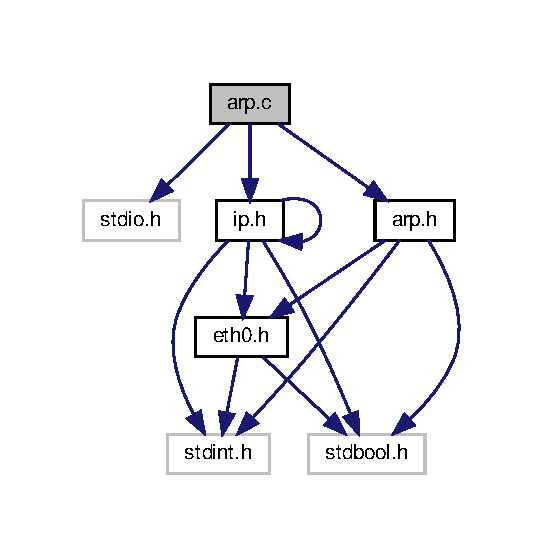
\includegraphics[width=261pt]{arp_8c__incl}
\end{center}
\end{figure}
\subsection*{Functions}
\begin{DoxyCompactItemize}
\item 
bool \hyperlink{arp_8c_aee82f38db8f23e7500976767ff0b0801}{is\+Arp\+Request} (\hyperlink{eth0_8h_a592bdc9f1e029368efe61c7eab510635}{ether\+Header} $\ast$ether)
\item 
bool \hyperlink{arp_8c_ad778486396ed427f7a65916336ac529c}{is\+Arp\+Response} (\hyperlink{eth0_8h_a592bdc9f1e029368efe61c7eab510635}{ether\+Header} $\ast$ether)
\item 
void \hyperlink{arp_8c_a9268cc75de7c71024782126b605fed01}{send\+Arp\+Response} (\hyperlink{eth0_8h_a592bdc9f1e029368efe61c7eab510635}{ether\+Header} $\ast$ether)
\item 
void \hyperlink{arp_8c_ad6d840efc736fbd372f2f637f151848e}{send\+Arp\+Request} (\hyperlink{eth0_8h_a592bdc9f1e029368efe61c7eab510635}{ether\+Header} $\ast$ether, uint8\+\_\+t ip\+From\mbox{[}$\,$\mbox{]}, uint8\+\_\+t ip\+To\mbox{[}$\,$\mbox{]})
\end{DoxyCompactItemize}


\subsection{Function Documentation}
\mbox{\Hypertarget{arp_8c_aee82f38db8f23e7500976767ff0b0801}\label{arp_8c_aee82f38db8f23e7500976767ff0b0801}} 
\index{arp.\+c@{arp.\+c}!is\+Arp\+Request@{is\+Arp\+Request}}
\index{is\+Arp\+Request@{is\+Arp\+Request}!arp.\+c@{arp.\+c}}
\subsubsection{\texorpdfstring{is\+Arp\+Request()}{isArpRequest()}}
{\footnotesize\ttfamily bool is\+Arp\+Request (\begin{DoxyParamCaption}\item[{\hyperlink{eth0_8h_a592bdc9f1e029368efe61c7eab510635}{ether\+Header} $\ast$}]{ether }\end{DoxyParamCaption})}



Definition at line 36 of file arp.\+c.

Here is the call graph for this function\+:
\nopagebreak
\begin{figure}[H]
\begin{center}
\leavevmode
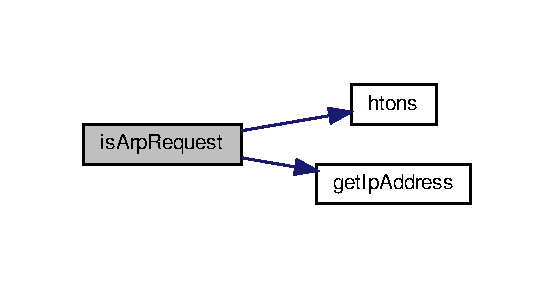
\includegraphics[width=266pt]{arp_8c_aee82f38db8f23e7500976767ff0b0801_cgraph}
\end{center}
\end{figure}
Here is the caller graph for this function\+:
\nopagebreak
\begin{figure}[H]
\begin{center}
\leavevmode
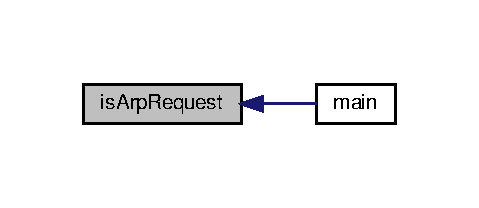
\includegraphics[width=230pt]{arp_8c_aee82f38db8f23e7500976767ff0b0801_icgraph}
\end{center}
\end{figure}
\mbox{\Hypertarget{arp_8c_ad778486396ed427f7a65916336ac529c}\label{arp_8c_ad778486396ed427f7a65916336ac529c}} 
\index{arp.\+c@{arp.\+c}!is\+Arp\+Response@{is\+Arp\+Response}}
\index{is\+Arp\+Response@{is\+Arp\+Response}!arp.\+c@{arp.\+c}}
\subsubsection{\texorpdfstring{is\+Arp\+Response()}{isArpResponse()}}
{\footnotesize\ttfamily bool is\+Arp\+Response (\begin{DoxyParamCaption}\item[{\hyperlink{eth0_8h_a592bdc9f1e029368efe61c7eab510635}{ether\+Header} $\ast$}]{ether }\end{DoxyParamCaption})}



Definition at line 55 of file arp.\+c.

Here is the call graph for this function\+:
\nopagebreak
\begin{figure}[H]
\begin{center}
\leavevmode
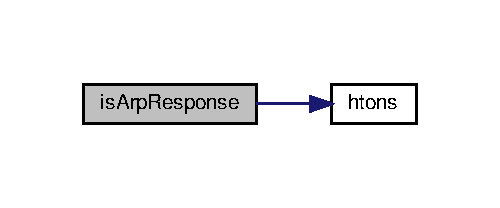
\includegraphics[width=240pt]{arp_8c_ad778486396ed427f7a65916336ac529c_cgraph}
\end{center}
\end{figure}
\mbox{\Hypertarget{arp_8c_ad6d840efc736fbd372f2f637f151848e}\label{arp_8c_ad6d840efc736fbd372f2f637f151848e}} 
\index{arp.\+c@{arp.\+c}!send\+Arp\+Request@{send\+Arp\+Request}}
\index{send\+Arp\+Request@{send\+Arp\+Request}!arp.\+c@{arp.\+c}}
\subsubsection{\texorpdfstring{send\+Arp\+Request()}{sendArpRequest()}}
{\footnotesize\ttfamily void send\+Arp\+Request (\begin{DoxyParamCaption}\item[{\hyperlink{eth0_8h_a592bdc9f1e029368efe61c7eab510635}{ether\+Header} $\ast$}]{ether,  }\item[{uint8\+\_\+t}]{ip\+From\mbox{[}$\,$\mbox{]},  }\item[{uint8\+\_\+t}]{ip\+To\mbox{[}$\,$\mbox{]} }\end{DoxyParamCaption})}



Definition at line 93 of file arp.\+c.

Here is the call graph for this function\+:
\nopagebreak
\begin{figure}[H]
\begin{center}
\leavevmode
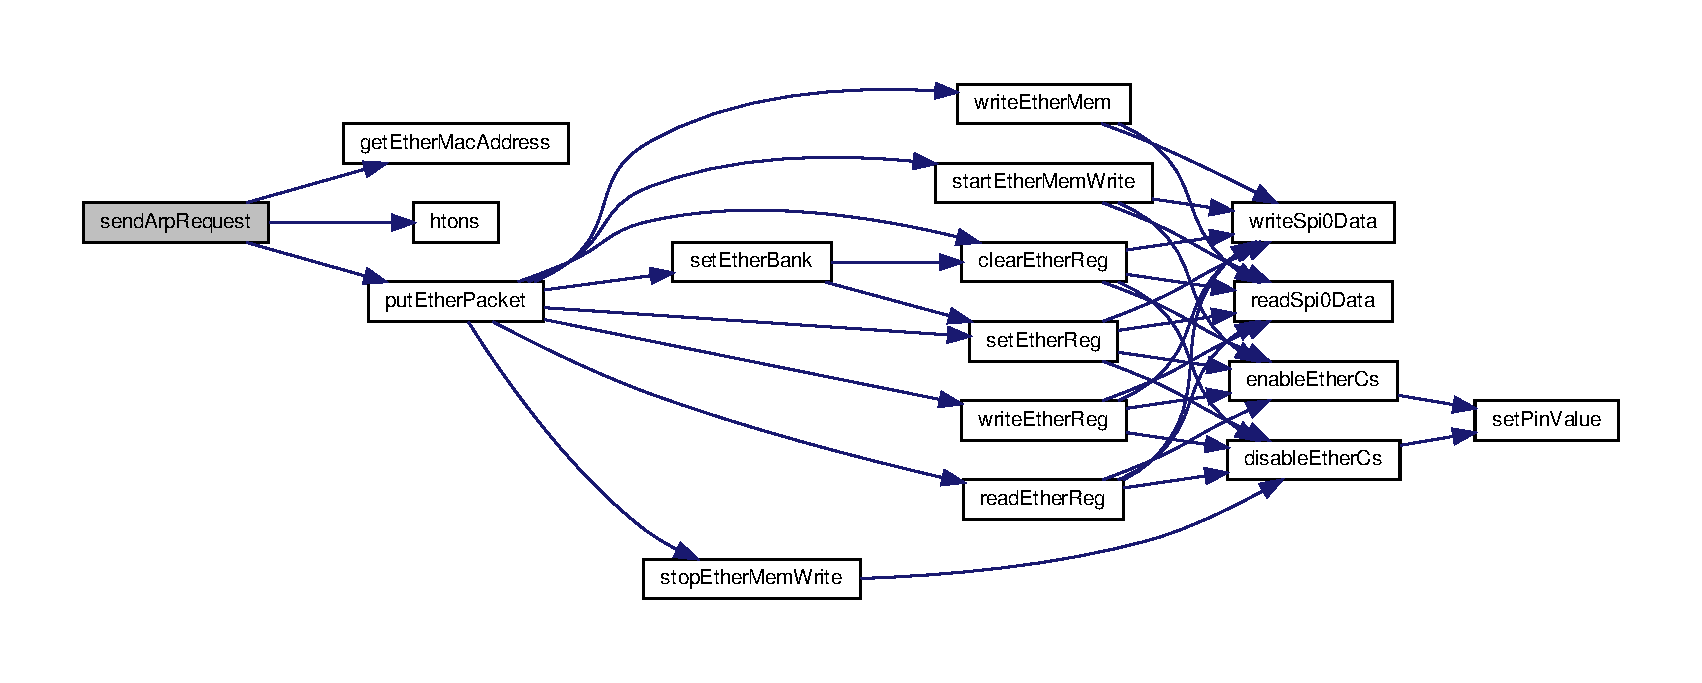
\includegraphics[width=350pt]{arp_8c_ad6d840efc736fbd372f2f637f151848e_cgraph}
\end{center}
\end{figure}
Here is the caller graph for this function\+:
\nopagebreak
\begin{figure}[H]
\begin{center}
\leavevmode
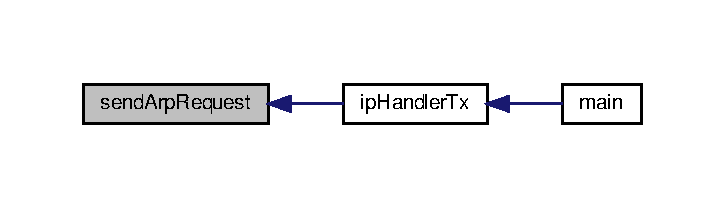
\includegraphics[width=348pt]{arp_8c_ad6d840efc736fbd372f2f637f151848e_icgraph}
\end{center}
\end{figure}
\mbox{\Hypertarget{arp_8c_a9268cc75de7c71024782126b605fed01}\label{arp_8c_a9268cc75de7c71024782126b605fed01}} 
\index{arp.\+c@{arp.\+c}!send\+Arp\+Response@{send\+Arp\+Response}}
\index{send\+Arp\+Response@{send\+Arp\+Response}!arp.\+c@{arp.\+c}}
\subsubsection{\texorpdfstring{send\+Arp\+Response()}{sendArpResponse()}}
{\footnotesize\ttfamily void send\+Arp\+Response (\begin{DoxyParamCaption}\item[{\hyperlink{eth0_8h_a592bdc9f1e029368efe61c7eab510635}{ether\+Header} $\ast$}]{ether }\end{DoxyParamCaption})}



Definition at line 66 of file arp.\+c.

Here is the call graph for this function\+:
\nopagebreak
\begin{figure}[H]
\begin{center}
\leavevmode
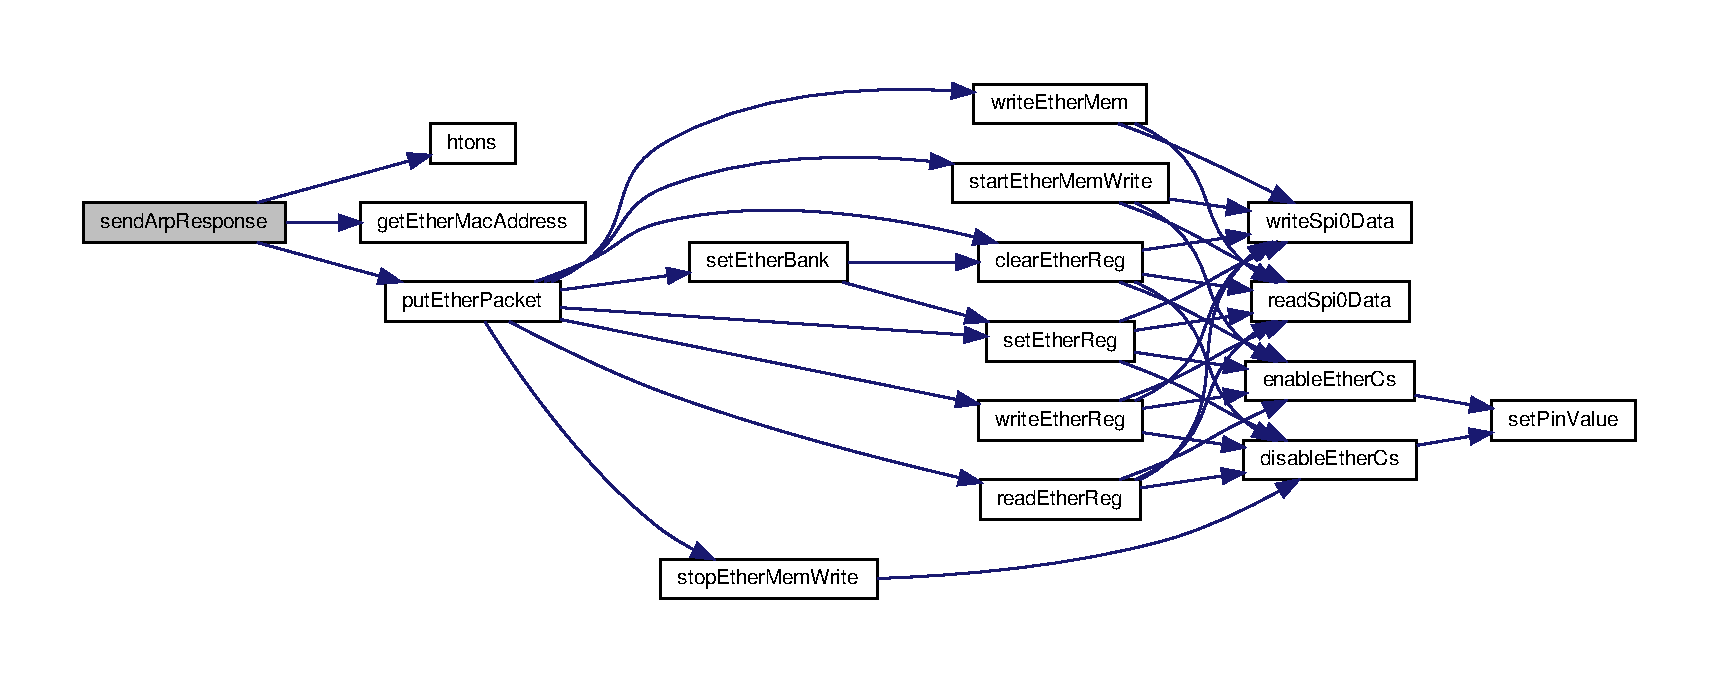
\includegraphics[width=350pt]{arp_8c_a9268cc75de7c71024782126b605fed01_cgraph}
\end{center}
\end{figure}
Here is the caller graph for this function\+:
\nopagebreak
\begin{figure}[H]
\begin{center}
\leavevmode
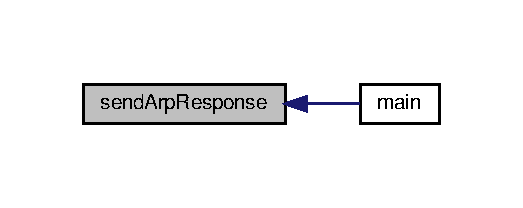
\includegraphics[width=251pt]{arp_8c_a9268cc75de7c71024782126b605fed01_icgraph}
\end{center}
\end{figure}

\hypertarget{arp_8h}{}\section{arp.\+h File Reference}
\label{arp_8h}\index{arp.\+h@{arp.\+h}}
{\ttfamily \#include $<$stdint.\+h$>$}\newline
{\ttfamily \#include $<$stdbool.\+h$>$}\newline
{\ttfamily \#include \char`\"{}eth0.\+h\char`\"{}}\newline
Include dependency graph for arp.\+h\+:
\nopagebreak
\begin{figure}[H]
\begin{center}
\leavevmode
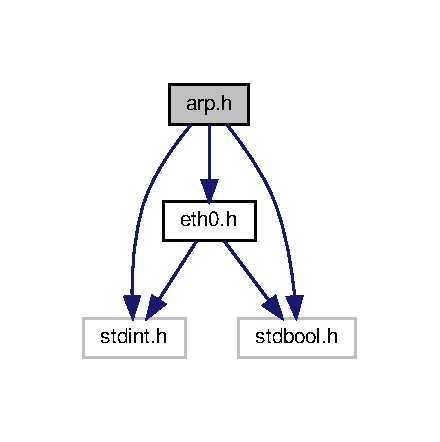
\includegraphics[width=211pt]{arp_8h__incl}
\end{center}
\end{figure}
This graph shows which files directly or indirectly include this file\+:
\nopagebreak
\begin{figure}[H]
\begin{center}
\leavevmode
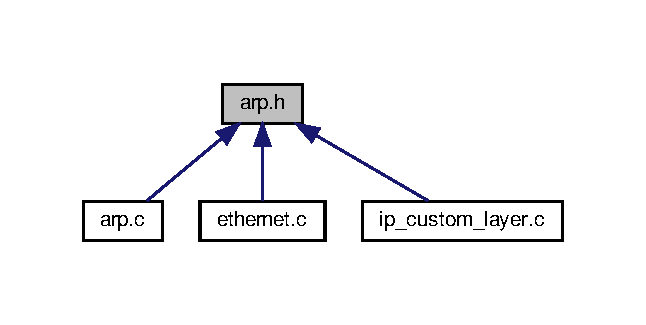
\includegraphics[width=310pt]{arp_8h__dep__incl}
\end{center}
\end{figure}
\subsection*{Data Structures}
\begin{DoxyCompactItemize}
\item 
struct \hyperlink{struct__arpPacket}{\+\_\+arp\+Packet}
\end{DoxyCompactItemize}
\subsection*{Typedefs}
\begin{DoxyCompactItemize}
\item 
typedef struct \hyperlink{struct__arpPacket}{\+\_\+arp\+Packet} \hyperlink{arp_8h_ac9a9fb6610c36c0008bacfad55d414f3}{arp\+Packet}
\end{DoxyCompactItemize}
\subsection*{Functions}
\begin{DoxyCompactItemize}
\item 
bool \hyperlink{arp_8h_aee82f38db8f23e7500976767ff0b0801}{is\+Arp\+Request} (\hyperlink{eth0_8h_a592bdc9f1e029368efe61c7eab510635}{ether\+Header} $\ast$ether)
\item 
bool \hyperlink{arp_8h_ad778486396ed427f7a65916336ac529c}{is\+Arp\+Response} (\hyperlink{eth0_8h_a592bdc9f1e029368efe61c7eab510635}{ether\+Header} $\ast$ether)
\item 
void \hyperlink{arp_8h_a9268cc75de7c71024782126b605fed01}{send\+Arp\+Response} (\hyperlink{eth0_8h_a592bdc9f1e029368efe61c7eab510635}{ether\+Header} $\ast$ether)
\item 
void \hyperlink{arp_8h_ad6d840efc736fbd372f2f637f151848e}{send\+Arp\+Request} (\hyperlink{eth0_8h_a592bdc9f1e029368efe61c7eab510635}{ether\+Header} $\ast$ether, uint8\+\_\+t ip\+From\mbox{[}$\,$\mbox{]}, uint8\+\_\+t ip\+To\mbox{[}$\,$\mbox{]})
\end{DoxyCompactItemize}


\subsection{Typedef Documentation}
\mbox{\Hypertarget{arp_8h_ac9a9fb6610c36c0008bacfad55d414f3}\label{arp_8h_ac9a9fb6610c36c0008bacfad55d414f3}} 
\index{arp.\+h@{arp.\+h}!arp\+Packet@{arp\+Packet}}
\index{arp\+Packet@{arp\+Packet}!arp.\+h@{arp.\+h}}
\subsubsection{\texorpdfstring{arp\+Packet}{arpPacket}}
{\footnotesize\ttfamily typedef struct \hyperlink{struct__arpPacket}{\+\_\+arp\+Packet}  \hyperlink{arp_8h_ac9a9fb6610c36c0008bacfad55d414f3}{arp\+Packet}}



\subsection{Function Documentation}
\mbox{\Hypertarget{arp_8h_aee82f38db8f23e7500976767ff0b0801}\label{arp_8h_aee82f38db8f23e7500976767ff0b0801}} 
\index{arp.\+h@{arp.\+h}!is\+Arp\+Request@{is\+Arp\+Request}}
\index{is\+Arp\+Request@{is\+Arp\+Request}!arp.\+h@{arp.\+h}}
\subsubsection{\texorpdfstring{is\+Arp\+Request()}{isArpRequest()}}
{\footnotesize\ttfamily bool is\+Arp\+Request (\begin{DoxyParamCaption}\item[{\hyperlink{eth0_8h_a592bdc9f1e029368efe61c7eab510635}{ether\+Header} $\ast$}]{ether }\end{DoxyParamCaption})}



Definition at line 36 of file arp.\+c.

Here is the call graph for this function\+:
\nopagebreak
\begin{figure}[H]
\begin{center}
\leavevmode
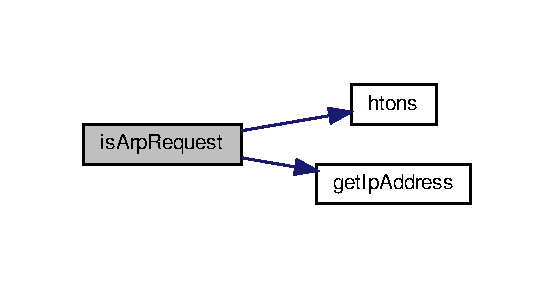
\includegraphics[width=266pt]{arp_8h_aee82f38db8f23e7500976767ff0b0801_cgraph}
\end{center}
\end{figure}
Here is the caller graph for this function\+:
\nopagebreak
\begin{figure}[H]
\begin{center}
\leavevmode
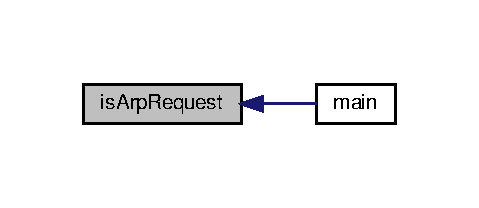
\includegraphics[width=230pt]{arp_8h_aee82f38db8f23e7500976767ff0b0801_icgraph}
\end{center}
\end{figure}
\mbox{\Hypertarget{arp_8h_ad778486396ed427f7a65916336ac529c}\label{arp_8h_ad778486396ed427f7a65916336ac529c}} 
\index{arp.\+h@{arp.\+h}!is\+Arp\+Response@{is\+Arp\+Response}}
\index{is\+Arp\+Response@{is\+Arp\+Response}!arp.\+h@{arp.\+h}}
\subsubsection{\texorpdfstring{is\+Arp\+Response()}{isArpResponse()}}
{\footnotesize\ttfamily bool is\+Arp\+Response (\begin{DoxyParamCaption}\item[{\hyperlink{eth0_8h_a592bdc9f1e029368efe61c7eab510635}{ether\+Header} $\ast$}]{ether }\end{DoxyParamCaption})}



Definition at line 55 of file arp.\+c.

Here is the call graph for this function\+:
\nopagebreak
\begin{figure}[H]
\begin{center}
\leavevmode
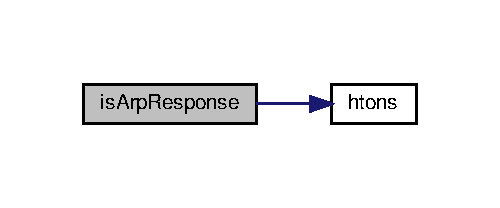
\includegraphics[width=240pt]{arp_8h_ad778486396ed427f7a65916336ac529c_cgraph}
\end{center}
\end{figure}
\mbox{\Hypertarget{arp_8h_ad6d840efc736fbd372f2f637f151848e}\label{arp_8h_ad6d840efc736fbd372f2f637f151848e}} 
\index{arp.\+h@{arp.\+h}!send\+Arp\+Request@{send\+Arp\+Request}}
\index{send\+Arp\+Request@{send\+Arp\+Request}!arp.\+h@{arp.\+h}}
\subsubsection{\texorpdfstring{send\+Arp\+Request()}{sendArpRequest()}}
{\footnotesize\ttfamily void send\+Arp\+Request (\begin{DoxyParamCaption}\item[{\hyperlink{eth0_8h_a592bdc9f1e029368efe61c7eab510635}{ether\+Header} $\ast$}]{ether,  }\item[{uint8\+\_\+t}]{ip\+From\mbox{[}$\,$\mbox{]},  }\item[{uint8\+\_\+t}]{ip\+To\mbox{[}$\,$\mbox{]} }\end{DoxyParamCaption})}



Definition at line 93 of file arp.\+c.

Here is the call graph for this function\+:
\nopagebreak
\begin{figure}[H]
\begin{center}
\leavevmode
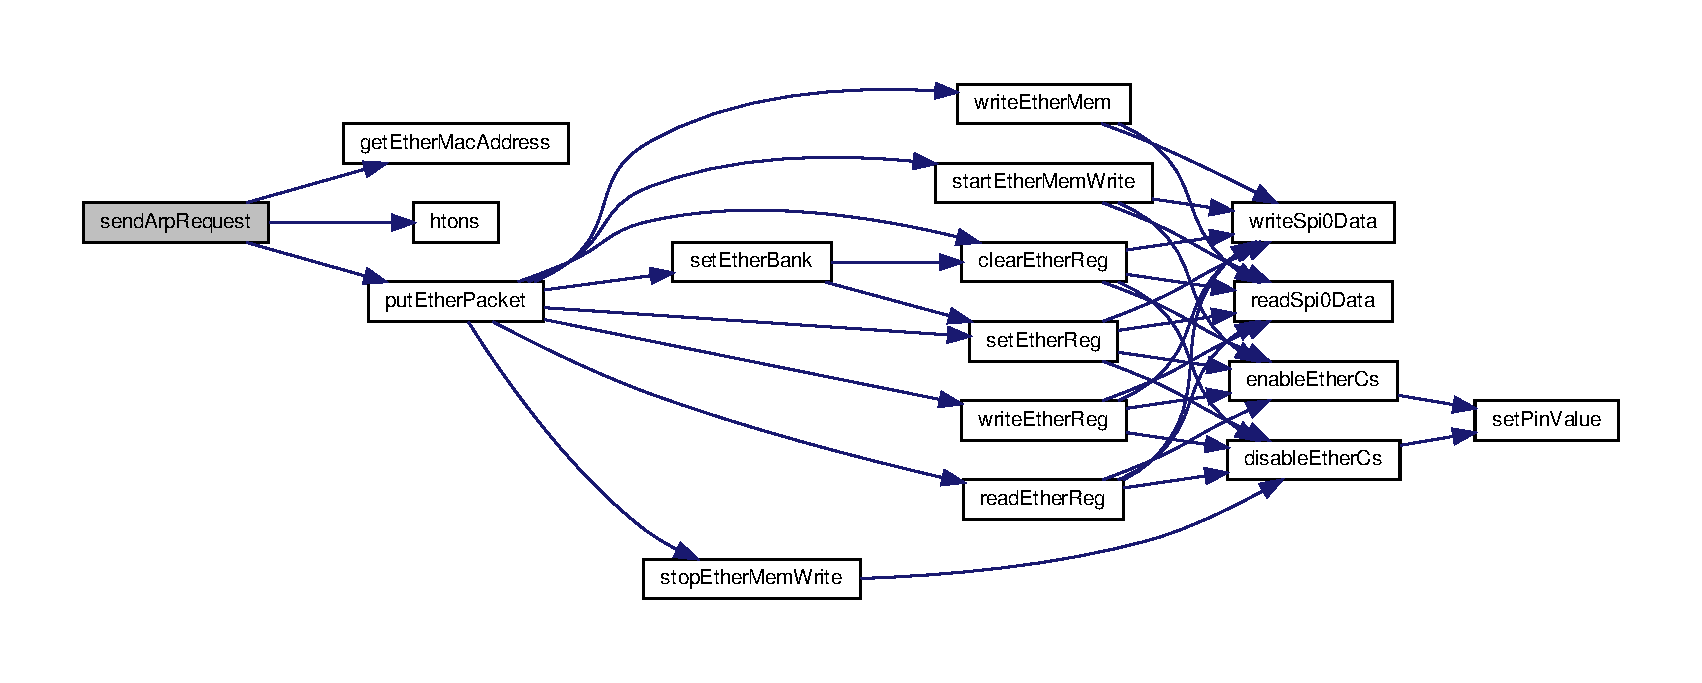
\includegraphics[width=350pt]{arp_8h_ad6d840efc736fbd372f2f637f151848e_cgraph}
\end{center}
\end{figure}
Here is the caller graph for this function\+:
\nopagebreak
\begin{figure}[H]
\begin{center}
\leavevmode
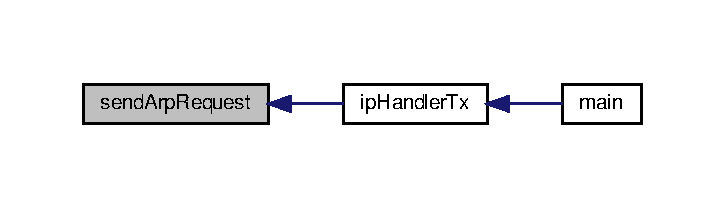
\includegraphics[width=348pt]{arp_8h_ad6d840efc736fbd372f2f637f151848e_icgraph}
\end{center}
\end{figure}
\mbox{\Hypertarget{arp_8h_a9268cc75de7c71024782126b605fed01}\label{arp_8h_a9268cc75de7c71024782126b605fed01}} 
\index{arp.\+h@{arp.\+h}!send\+Arp\+Response@{send\+Arp\+Response}}
\index{send\+Arp\+Response@{send\+Arp\+Response}!arp.\+h@{arp.\+h}}
\subsubsection{\texorpdfstring{send\+Arp\+Response()}{sendArpResponse()}}
{\footnotesize\ttfamily void send\+Arp\+Response (\begin{DoxyParamCaption}\item[{\hyperlink{eth0_8h_a592bdc9f1e029368efe61c7eab510635}{ether\+Header} $\ast$}]{ether }\end{DoxyParamCaption})}



Definition at line 66 of file arp.\+c.

Here is the call graph for this function\+:
\nopagebreak
\begin{figure}[H]
\begin{center}
\leavevmode
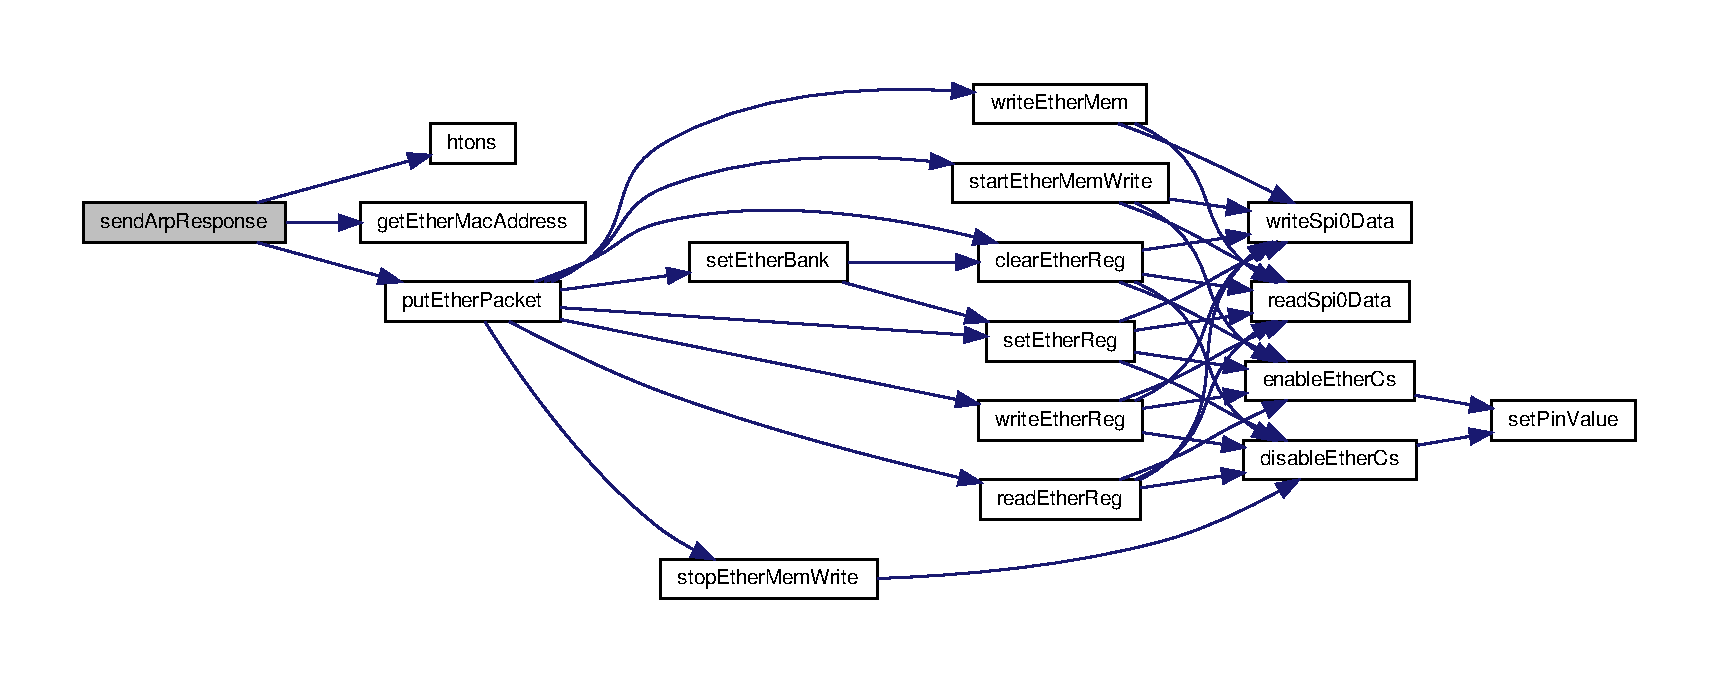
\includegraphics[width=350pt]{arp_8h_a9268cc75de7c71024782126b605fed01_cgraph}
\end{center}
\end{figure}
Here is the caller graph for this function\+:
\nopagebreak
\begin{figure}[H]
\begin{center}
\leavevmode
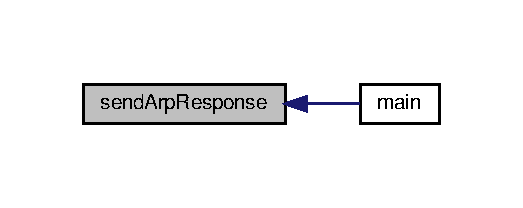
\includegraphics[width=251pt]{arp_8h_a9268cc75de7c71024782126b605fed01_icgraph}
\end{center}
\end{figure}

\hypertarget{clock_8c}{}\section{clock.\+c File Reference}
\label{clock_8c}\index{clock.\+c@{clock.\+c}}
{\ttfamily \#include $<$stdint.\+h$>$}\newline
{\ttfamily \#include \char`\"{}clock.\+h\char`\"{}}\newline
{\ttfamily \#include \char`\"{}tm4c123gh6pm.\+h\char`\"{}}\newline
Include dependency graph for clock.\+c\+:
\nopagebreak
\begin{figure}[H]
\begin{center}
\leavevmode
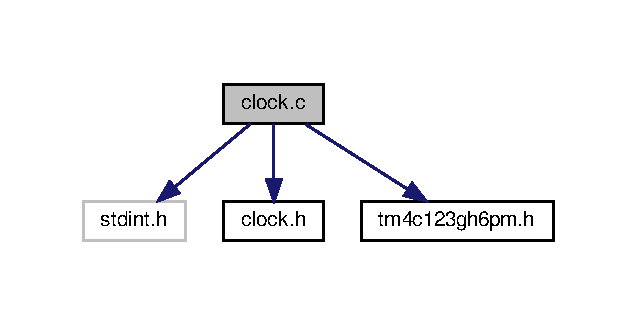
\includegraphics[width=306pt]{clock_8c__incl}
\end{center}
\end{figure}
\subsection*{Functions}
\begin{DoxyCompactItemize}
\item 
void \hyperlink{clock_8c_a4286103d9ce0891f14b8c51f1c023da3}{init\+System\+Clock\+To40\+Mhz} (void)
\end{DoxyCompactItemize}


\subsection{Function Documentation}
\mbox{\Hypertarget{clock_8c_a4286103d9ce0891f14b8c51f1c023da3}\label{clock_8c_a4286103d9ce0891f14b8c51f1c023da3}} 
\index{clock.\+c@{clock.\+c}!init\+System\+Clock\+To40\+Mhz@{init\+System\+Clock\+To40\+Mhz}}
\index{init\+System\+Clock\+To40\+Mhz@{init\+System\+Clock\+To40\+Mhz}!clock.\+c@{clock.\+c}}
\subsubsection{\texorpdfstring{init\+System\+Clock\+To40\+Mhz()}{initSystemClockTo40Mhz()}}
{\footnotesize\ttfamily void init\+System\+Clock\+To40\+Mhz (\begin{DoxyParamCaption}\item[{void}]{ }\end{DoxyParamCaption})}



Definition at line 32 of file clock.\+c.

Here is the caller graph for this function\+:
\nopagebreak
\begin{figure}[H]
\begin{center}
\leavevmode
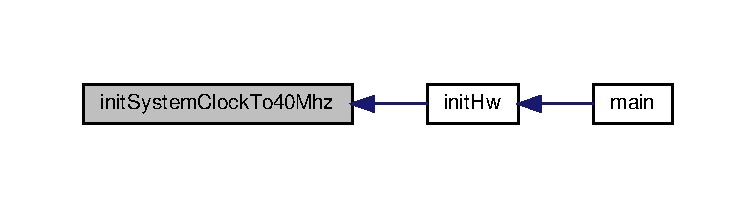
\includegraphics[width=350pt]{clock_8c_a4286103d9ce0891f14b8c51f1c023da3_icgraph}
\end{center}
\end{figure}

\hypertarget{clock_8h}{}\section{clock.\+h File Reference}
\label{clock_8h}\index{clock.\+h@{clock.\+h}}
This graph shows which files directly or indirectly include this file\+:
\nopagebreak
\begin{figure}[H]
\begin{center}
\leavevmode
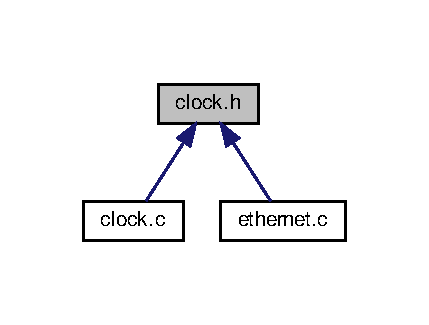
\includegraphics[width=206pt]{clock_8h__dep__incl}
\end{center}
\end{figure}
\subsection*{Functions}
\begin{DoxyCompactItemize}
\item 
void \hyperlink{clock_8h_a4286103d9ce0891f14b8c51f1c023da3}{init\+System\+Clock\+To40\+Mhz} (void)
\end{DoxyCompactItemize}


\subsection{Function Documentation}
\mbox{\Hypertarget{clock_8h_a4286103d9ce0891f14b8c51f1c023da3}\label{clock_8h_a4286103d9ce0891f14b8c51f1c023da3}} 
\index{clock.\+h@{clock.\+h}!init\+System\+Clock\+To40\+Mhz@{init\+System\+Clock\+To40\+Mhz}}
\index{init\+System\+Clock\+To40\+Mhz@{init\+System\+Clock\+To40\+Mhz}!clock.\+h@{clock.\+h}}
\subsubsection{\texorpdfstring{init\+System\+Clock\+To40\+Mhz()}{initSystemClockTo40Mhz()}}
{\footnotesize\ttfamily void init\+System\+Clock\+To40\+Mhz (\begin{DoxyParamCaption}\item[{void}]{ }\end{DoxyParamCaption})}



Definition at line 32 of file clock.\+c.

Here is the caller graph for this function\+:
\nopagebreak
\begin{figure}[H]
\begin{center}
\leavevmode
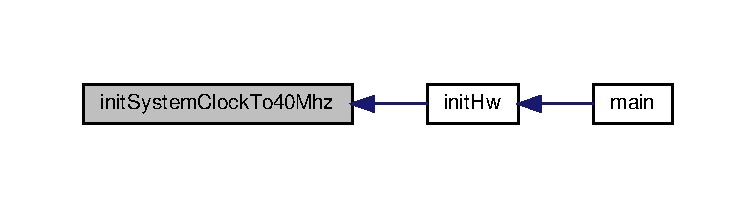
\includegraphics[width=350pt]{clock_8h_a4286103d9ce0891f14b8c51f1c023da3_icgraph}
\end{center}
\end{figure}

\hypertarget{arp_8d}{}\section{Debug/arp.d File Reference}
\label{arp_8d}\index{Debug/arp.\+d@{Debug/arp.\+d}}

\hypertarget{clock_8d}{}\section{Debug/clock.d File Reference}
\label{clock_8d}\index{Debug/clock.\+d@{Debug/clock.\+d}}

\hypertarget{commandline_8d}{}\section{Debug/commandline.d File Reference}
\label{commandline_8d}\index{Debug/commandline.\+d@{Debug/commandline.\+d}}

\hypertarget{eeprom_8d}{}\section{Debug/eeprom.d File Reference}
\label{eeprom_8d}\index{Debug/eeprom.\+d@{Debug/eeprom.\+d}}

\hypertarget{eth0_8d}{}\section{Debug/eth0.d File Reference}
\label{eth0_8d}\index{Debug/eth0.\+d@{Debug/eth0.\+d}}

\hypertarget{ethernet_8d}{}\section{Debug/ethernet.d File Reference}
\label{ethernet_8d}\index{Debug/ethernet.\+d@{Debug/ethernet.\+d}}

\hypertarget{gpio_8d}{}\section{Debug/gpio.d File Reference}
\label{gpio_8d}\index{Debug/gpio.\+d@{Debug/gpio.\+d}}

\hypertarget{icmp_8d}{}\section{Debug/icmp.d File Reference}
\label{icmp_8d}\index{Debug/icmp.\+d@{Debug/icmp.\+d}}

\hypertarget{ip_8d}{}\section{Debug/ip.d File Reference}
\label{ip_8d}\index{Debug/ip.\+d@{Debug/ip.\+d}}

\hypertarget{ip__custom__layer_8d}{}\section{Debug/ip\+\_\+custom\+\_\+layer.d File Reference}
\label{ip__custom__layer_8d}\index{Debug/ip\+\_\+custom\+\_\+layer.\+d@{Debug/ip\+\_\+custom\+\_\+layer.\+d}}

\hypertarget{mqtt_8d}{}\section{Debug/mqtt.d File Reference}
\label{mqtt_8d}\index{Debug/mqtt.\+d@{Debug/mqtt.\+d}}

\hypertarget{spi0_8d}{}\section{Debug/spi0.d File Reference}
\label{spi0_8d}\index{Debug/spi0.\+d@{Debug/spi0.\+d}}

\hypertarget{tcp_8d}{}\section{Debug/tcp.d File Reference}
\label{tcp_8d}\index{Debug/tcp.\+d@{Debug/tcp.\+d}}

\hypertarget{timer_8d}{}\section{Debug/timer.d File Reference}
\label{timer_8d}\index{Debug/timer.\+d@{Debug/timer.\+d}}

\hypertarget{tm4c123gh6pm__startup__ccs_8d}{}\section{Debug/tm4c123gh6pm\+\_\+startup\+\_\+ccs.d File Reference}
\label{tm4c123gh6pm__startup__ccs_8d}\index{Debug/tm4c123gh6pm\+\_\+startup\+\_\+ccs.\+d@{Debug/tm4c123gh6pm\+\_\+startup\+\_\+ccs.\+d}}

\hypertarget{uart0_8d}{}\section{Debug/uart0.d File Reference}
\label{uart0_8d}\index{Debug/uart0.\+d@{Debug/uart0.\+d}}

\hypertarget{udp_8d}{}\section{Debug/udp.d File Reference}
\label{udp_8d}\index{Debug/udp.\+d@{Debug/udp.\+d}}

\hypertarget{wait_8d}{}\section{Debug/wait.d File Reference}
\label{wait_8d}\index{Debug/wait.\+d@{Debug/wait.\+d}}

\hypertarget{eeprom_8c}{}\section{eeprom.\+c File Reference}
\label{eeprom_8c}\index{eeprom.\+c@{eeprom.\+c}}
{\ttfamily \#include $<$stdint.\+h$>$}\newline
{\ttfamily \#include \char`\"{}tm4c123gh6pm.\+h\char`\"{}}\newline
{\ttfamily \#include \char`\"{}eeprom.\+h\char`\"{}}\newline
Include dependency graph for eeprom.\+c\+:
\nopagebreak
\begin{figure}[H]
\begin{center}
\leavevmode
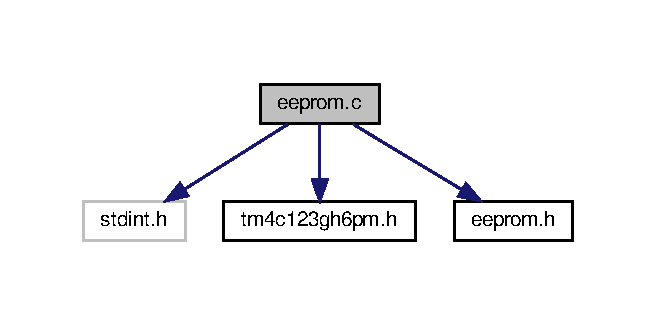
\includegraphics[width=315pt]{eeprom_8c__incl}
\end{center}
\end{figure}
\subsection*{Functions}
\begin{DoxyCompactItemize}
\item 
void \hyperlink{eeprom_8c_a4730a45291a8fa090e9c9b3a0fd10cab}{init\+Eeprom} (void)
\item 
void \hyperlink{eeprom_8c_ad5263b15f0ad67de6b49e26347ad01e0}{write\+Eeprom} (uint16\+\_\+t add, uint32\+\_\+t data)
\item 
uint32\+\_\+t \hyperlink{eeprom_8c_ae2498080898399278f2bb70a8987118a}{read\+Eeprom} (uint16\+\_\+t add)
\end{DoxyCompactItemize}


\subsection{Function Documentation}
\mbox{\Hypertarget{eeprom_8c_a4730a45291a8fa090e9c9b3a0fd10cab}\label{eeprom_8c_a4730a45291a8fa090e9c9b3a0fd10cab}} 
\index{eeprom.\+c@{eeprom.\+c}!init\+Eeprom@{init\+Eeprom}}
\index{init\+Eeprom@{init\+Eeprom}!eeprom.\+c@{eeprom.\+c}}
\subsubsection{\texorpdfstring{init\+Eeprom()}{initEeprom()}}
{\footnotesize\ttfamily void init\+Eeprom (\begin{DoxyParamCaption}\item[{void}]{ }\end{DoxyParamCaption})}



Definition at line 23 of file eeprom.\+c.

Here is the caller graph for this function\+:
\nopagebreak
\begin{figure}[H]
\begin{center}
\leavevmode
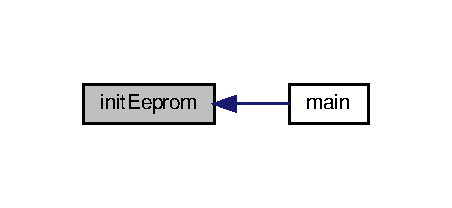
\includegraphics[width=217pt]{eeprom_8c_a4730a45291a8fa090e9c9b3a0fd10cab_icgraph}
\end{center}
\end{figure}
\mbox{\Hypertarget{eeprom_8c_ae2498080898399278f2bb70a8987118a}\label{eeprom_8c_ae2498080898399278f2bb70a8987118a}} 
\index{eeprom.\+c@{eeprom.\+c}!read\+Eeprom@{read\+Eeprom}}
\index{read\+Eeprom@{read\+Eeprom}!eeprom.\+c@{eeprom.\+c}}
\subsubsection{\texorpdfstring{read\+Eeprom()}{readEeprom()}}
{\footnotesize\ttfamily uint32\+\_\+t read\+Eeprom (\begin{DoxyParamCaption}\item[{uint16\+\_\+t}]{add }\end{DoxyParamCaption})}



Definition at line 38 of file eeprom.\+c.

Here is the caller graph for this function\+:
\nopagebreak
\begin{figure}[H]
\begin{center}
\leavevmode
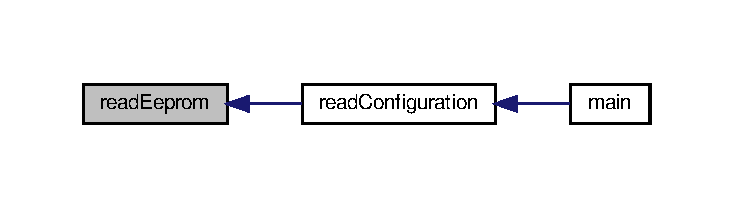
\includegraphics[width=350pt]{eeprom_8c_ae2498080898399278f2bb70a8987118a_icgraph}
\end{center}
\end{figure}
\mbox{\Hypertarget{eeprom_8c_ad5263b15f0ad67de6b49e26347ad01e0}\label{eeprom_8c_ad5263b15f0ad67de6b49e26347ad01e0}} 
\index{eeprom.\+c@{eeprom.\+c}!write\+Eeprom@{write\+Eeprom}}
\index{write\+Eeprom@{write\+Eeprom}!eeprom.\+c@{eeprom.\+c}}
\subsubsection{\texorpdfstring{write\+Eeprom()}{writeEeprom()}}
{\footnotesize\ttfamily void write\+Eeprom (\begin{DoxyParamCaption}\item[{uint16\+\_\+t}]{add,  }\item[{uint32\+\_\+t}]{data }\end{DoxyParamCaption})}



Definition at line 30 of file eeprom.\+c.

Here is the caller graph for this function\+:
\nopagebreak
\begin{figure}[H]
\begin{center}
\leavevmode
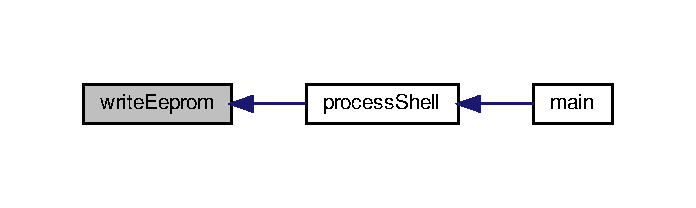
\includegraphics[width=334pt]{eeprom_8c_ad5263b15f0ad67de6b49e26347ad01e0_icgraph}
\end{center}
\end{figure}

\hypertarget{eeprom_8h}{}\section{eeprom.\+h File Reference}
\label{eeprom_8h}\index{eeprom.\+h@{eeprom.\+h}}
This graph shows which files directly or indirectly include this file\+:
\nopagebreak
\begin{figure}[H]
\begin{center}
\leavevmode
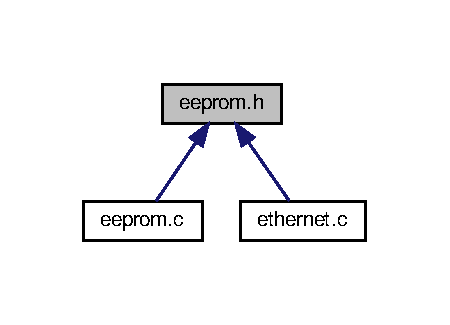
\includegraphics[width=216pt]{eeprom_8h__dep__incl}
\end{center}
\end{figure}
\subsection*{Functions}
\begin{DoxyCompactItemize}
\item 
void \hyperlink{eeprom_8h_a4730a45291a8fa090e9c9b3a0fd10cab}{init\+Eeprom} (void)
\item 
void \hyperlink{eeprom_8h_ad5263b15f0ad67de6b49e26347ad01e0}{write\+Eeprom} (uint16\+\_\+t add, uint32\+\_\+t data)
\item 
uint32\+\_\+t \hyperlink{eeprom_8h_ae2498080898399278f2bb70a8987118a}{read\+Eeprom} (uint16\+\_\+t add)
\end{DoxyCompactItemize}


\subsection{Function Documentation}
\mbox{\Hypertarget{eeprom_8h_a4730a45291a8fa090e9c9b3a0fd10cab}\label{eeprom_8h_a4730a45291a8fa090e9c9b3a0fd10cab}} 
\index{eeprom.\+h@{eeprom.\+h}!init\+Eeprom@{init\+Eeprom}}
\index{init\+Eeprom@{init\+Eeprom}!eeprom.\+h@{eeprom.\+h}}
\subsubsection{\texorpdfstring{init\+Eeprom()}{initEeprom()}}
{\footnotesize\ttfamily void init\+Eeprom (\begin{DoxyParamCaption}\item[{void}]{ }\end{DoxyParamCaption})}



Definition at line 23 of file eeprom.\+c.

Here is the caller graph for this function\+:
\nopagebreak
\begin{figure}[H]
\begin{center}
\leavevmode
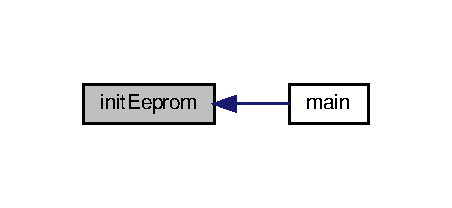
\includegraphics[width=217pt]{eeprom_8h_a4730a45291a8fa090e9c9b3a0fd10cab_icgraph}
\end{center}
\end{figure}
\mbox{\Hypertarget{eeprom_8h_ae2498080898399278f2bb70a8987118a}\label{eeprom_8h_ae2498080898399278f2bb70a8987118a}} 
\index{eeprom.\+h@{eeprom.\+h}!read\+Eeprom@{read\+Eeprom}}
\index{read\+Eeprom@{read\+Eeprom}!eeprom.\+h@{eeprom.\+h}}
\subsubsection{\texorpdfstring{read\+Eeprom()}{readEeprom()}}
{\footnotesize\ttfamily uint32\+\_\+t read\+Eeprom (\begin{DoxyParamCaption}\item[{uint16\+\_\+t}]{add }\end{DoxyParamCaption})}



Definition at line 38 of file eeprom.\+c.

Here is the caller graph for this function\+:
\nopagebreak
\begin{figure}[H]
\begin{center}
\leavevmode
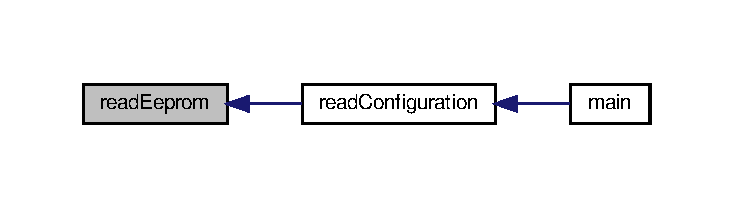
\includegraphics[width=350pt]{eeprom_8h_ae2498080898399278f2bb70a8987118a_icgraph}
\end{center}
\end{figure}
\mbox{\Hypertarget{eeprom_8h_ad5263b15f0ad67de6b49e26347ad01e0}\label{eeprom_8h_ad5263b15f0ad67de6b49e26347ad01e0}} 
\index{eeprom.\+h@{eeprom.\+h}!write\+Eeprom@{write\+Eeprom}}
\index{write\+Eeprom@{write\+Eeprom}!eeprom.\+h@{eeprom.\+h}}
\subsubsection{\texorpdfstring{write\+Eeprom()}{writeEeprom()}}
{\footnotesize\ttfamily void write\+Eeprom (\begin{DoxyParamCaption}\item[{uint16\+\_\+t}]{add,  }\item[{uint32\+\_\+t}]{data }\end{DoxyParamCaption})}



Definition at line 30 of file eeprom.\+c.

Here is the caller graph for this function\+:
\nopagebreak
\begin{figure}[H]
\begin{center}
\leavevmode
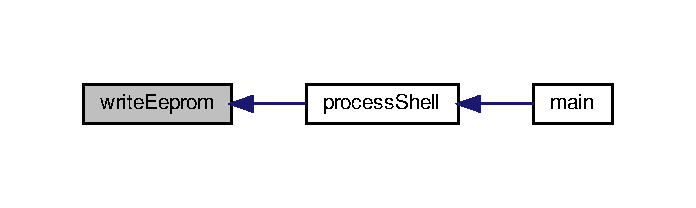
\includegraphics[width=334pt]{eeprom_8h_ad5263b15f0ad67de6b49e26347ad01e0_icgraph}
\end{center}
\end{figure}

\hypertarget{eth0_8c}{}\section{eth0.\+c File Reference}
\label{eth0_8c}\index{eth0.\+c@{eth0.\+c}}
{\ttfamily \#include $<$stdint.\+h$>$}\newline
{\ttfamily \#include $<$stdbool.\+h$>$}\newline
{\ttfamily \#include \char`\"{}tm4c123gh6pm.\+h\char`\"{}}\newline
{\ttfamily \#include \char`\"{}wait.\+h\char`\"{}}\newline
{\ttfamily \#include \char`\"{}gpio.\+h\char`\"{}}\newline
{\ttfamily \#include \char`\"{}spi0.\+h\char`\"{}}\newline
{\ttfamily \#include \char`\"{}eth0.\+h\char`\"{}}\newline
Include dependency graph for eth0.\+c\+:
\nopagebreak
\begin{figure}[H]
\begin{center}
\leavevmode
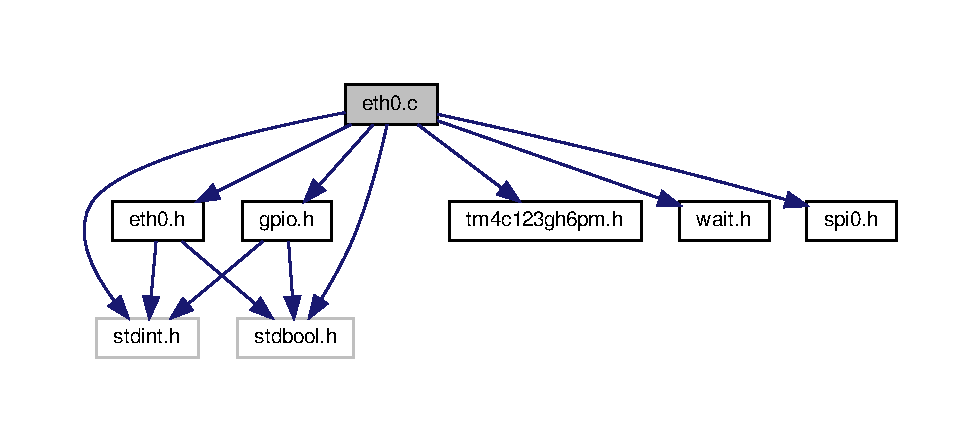
\includegraphics[width=350pt]{eth0_8c__incl}
\end{center}
\end{figure}
\subsection*{Macros}
\begin{DoxyCompactItemize}
\item 
\#define \hyperlink{eth0_8c_a3780e2fe762dc532df7d0f030b55caa0}{CS}~\hyperlink{gpio_8h_a26254f886d2dced3476c09635a7e5d5bae3201f6e0d0c1e138c60903276bb3859}{P\+O\+R\+TA},3
\item 
\#define \hyperlink{eth0_8c_a766daf7210b73953ce55988d8bd0e3b8}{W\+OL}~\hyperlink{gpio_8h_a26254f886d2dced3476c09635a7e5d5bae51dea4a37f3e2ede7ba6f27c563f6a4}{P\+O\+R\+TB},3
\item 
\#define \hyperlink{eth0_8c_afeeffe52c8fd59db7c61cf8b02042dbf}{I\+NT}~\hyperlink{gpio_8h_a26254f886d2dced3476c09635a7e5d5bafcec7c36cc8137e94db854fdec9d2d50}{P\+O\+R\+TC},6
\item 
\#define \hyperlink{eth0_8c_a04e5f3a270ebf2b1a1121b38fef2a62e}{E\+R\+D\+P\+TL}~0x00
\item 
\#define \hyperlink{eth0_8c_a63011487c82b6f6d1fcc749b55e5511e}{E\+R\+D\+P\+TH}~0x01
\item 
\#define \hyperlink{eth0_8c_a684dfa8cb9097ee131a2c9d2ee65d573}{E\+W\+R\+P\+TL}~0x02
\item 
\#define \hyperlink{eth0_8c_a7bda37d486623efbe3ac2055198d356a}{E\+W\+R\+P\+TH}~0x03
\item 
\#define \hyperlink{eth0_8c_a45a38712c4d618bb5cb013e3d781db46}{E\+T\+X\+S\+TL}~0x04
\item 
\#define \hyperlink{eth0_8c_adfc695618aa5a32160cc9e2b0234c714}{E\+T\+X\+S\+TH}~0x05
\item 
\#define \hyperlink{eth0_8c_ad79a19cc60b7dc19cec9df691e658714}{E\+T\+X\+N\+DL}~0x06
\item 
\#define \hyperlink{eth0_8c_a24597e8d914818adae20bf39c4ac7d0e}{E\+T\+X\+N\+DH}~0x07
\item 
\#define \hyperlink{eth0_8c_a387e1ac675539e1c0c7f158f59eafd51}{E\+R\+X\+S\+TL}~0x08
\item 
\#define \hyperlink{eth0_8c_ad4c2a40d74ded1e155f7eb18effb76ba}{E\+R\+X\+S\+TH}~0x09
\item 
\#define \hyperlink{eth0_8c_a9fa6592ccdfa66aa5a1854dd95b6329c}{E\+R\+X\+N\+DL}~0x0A
\item 
\#define \hyperlink{eth0_8c_a19ee05a22525dcd9e4124734a3aec1b0}{E\+R\+X\+N\+DH}~0x0B
\item 
\#define \hyperlink{eth0_8c_a0e4345b59cc531bd8daee2cd8c8e906b}{E\+R\+X\+R\+D\+P\+TL}~0x0C
\item 
\#define \hyperlink{eth0_8c_a1668b845f0bc37dbb515c2358357a690}{E\+R\+X\+R\+D\+P\+TH}~0x0D
\item 
\#define \hyperlink{eth0_8c_a7d78e648da085c6fdf006d75b3c99a7a}{E\+R\+X\+W\+R\+P\+TL}~0x0E
\item 
\#define \hyperlink{eth0_8c_a9c9ff6952a5cb0c0b420bc6a405d726c}{E\+R\+X\+W\+R\+P\+TH}~0x0F
\item 
\#define \hyperlink{eth0_8c_a72ac42db94893a565a52821f5ae95856}{E\+IE}~0x1B
\item 
\#define \hyperlink{eth0_8c_a303aba585a8da3f8dc80315dc94cb0e5}{E\+IR}~0x1C
\item 
\#define \hyperlink{eth0_8c_adb3411c72b313ba961c0cf775cf9db02}{R\+X\+E\+R\+IF}~0x01
\item 
\#define \hyperlink{eth0_8c_a7a0f9cb1aef73f027e31bd01426f2d7a}{T\+X\+E\+R\+IF}~0x02
\item 
\#define \hyperlink{eth0_8c_ac765fb3c77a3c11ddd4e7ac9ea7b4bed}{T\+X\+IF}~0x08
\item 
\#define \hyperlink{eth0_8c_a567e73e06d0b2569df3aa2c53c4540bb}{P\+K\+T\+IF}~0x40
\item 
\#define \hyperlink{eth0_8c_ad05043a04b51b3953259c24040e2e99f}{E\+S\+T\+AT}~0x1D
\item 
\#define \hyperlink{eth0_8c_ab8108f29c6eb17edb95d8e3e86269ae2}{C\+L\+K\+R\+DY}~0x01
\item 
\#define \hyperlink{eth0_8c_a6dae2de25c84b91c5d49a3145cf04305}{T\+X\+A\+B\+O\+RT}~0x02
\item 
\#define \hyperlink{eth0_8c_a86d77e305cc8d23f335fb733870a873c}{E\+C\+O\+N2}~0x1E
\item 
\#define \hyperlink{eth0_8c_a2749c0d85a8e2a2686eb6c05ccae2087}{P\+K\+T\+D\+EC}~0x40
\item 
\#define \hyperlink{eth0_8c_a461b29cd8a06dc2f331f664eb0f9165a}{E\+C\+O\+N1}~0x1F
\item 
\#define \hyperlink{eth0_8c_a5a1bf6f4852d0c813756b783ff285bab}{R\+X\+EN}~0x04
\item 
\#define \hyperlink{eth0_8c_ac97c83c67cb160908e4f640370155c2a}{T\+X\+R\+TS}~0x08
\item 
\#define \hyperlink{eth0_8c_ac5ff36d9b43977e5dd6548170ec93ddc}{E\+R\+X\+F\+C\+ON}~0x38
\item 
\#define \hyperlink{eth0_8c_a029f8b5f05e4e5182aa9a73e31c4a4f0}{E\+P\+K\+T\+C\+NT}~0x39
\item 
\#define \hyperlink{eth0_8c_ab64add14e73a7308bd32343c45caf79d}{M\+A\+C\+O\+N1}~0x40
\item 
\#define \hyperlink{eth0_8c_a5bafdeaf62f6f1040d02c76869a7e6ad}{M\+A\+R\+X\+EN}~0x01
\item 
\#define \hyperlink{eth0_8c_a13e2c5a266fa002bd903394ea9313708}{R\+X\+P\+A\+US}~0x04
\item 
\#define \hyperlink{eth0_8c_aa96ab16a2dddfccd77b723367e7d9acd}{T\+X\+P\+A\+US}~0x08
\item 
\#define \hyperlink{eth0_8c_a01501b400de6174cd44cd52cf9da0950}{M\+A\+C\+O\+N2}~0x41
\item 
\#define \hyperlink{eth0_8c_ac8c4de938f683881693704da4844c807}{M\+A\+R\+ST}~0x80
\item 
\#define \hyperlink{eth0_8c_a37e80f66673c39e7db383e0b11a159ea}{M\+A\+C\+O\+N3}~0x42
\item 
\#define \hyperlink{eth0_8c_a5349c2f5efe2df5d38830819f44393c9}{F\+U\+L\+D\+PX}~0x01
\item 
\#define \hyperlink{eth0_8c_a9ffd80c58ad749f063047912daf64748}{F\+R\+M\+L\+N\+EN}~0x02
\item 
\#define \hyperlink{eth0_8c_a835f9be221794e025cde45d42fe95794}{T\+X\+C\+R\+C\+EN}~0x10
\item 
\#define \hyperlink{eth0_8c_ab67a61415d9fda853ce94354a4b7c6a3}{P\+A\+D60}~0x20
\item 
\#define \hyperlink{eth0_8c_a53c0d8f74a3ba17d1337e297ef749a22}{M\+A\+C\+O\+N4}~0x43
\item 
\#define \hyperlink{eth0_8c_a0aa3bb65f69bc921f3b4020410f7efc2}{M\+A\+B\+B\+I\+PG}~0x44
\item 
\#define \hyperlink{eth0_8c_a8daa7f7ef529828ef4cc3d90a48ff730}{M\+A\+I\+P\+GL}~0x46
\item 
\#define \hyperlink{eth0_8c_a70b21ea01d623429bf3bd1abf583c80f}{M\+A\+I\+P\+GH}~0x47
\item 
\#define \hyperlink{eth0_8c_af78bae411a3ae7fe363ad63e93a2e618}{M\+A\+C\+L\+C\+O\+N1}~0x48
\item 
\#define \hyperlink{eth0_8c_acf3356546b7e518a4cf8b368d48a2710}{M\+A\+C\+L\+C\+O\+N2}~0x49
\item 
\#define \hyperlink{eth0_8c_a4ed708903a040c0ea4fc071707863ffc}{M\+A\+M\+X\+F\+LL}~0x4A
\item 
\#define \hyperlink{eth0_8c_a294e961d04adc72cbc8b866bb6506e8d}{M\+A\+M\+X\+F\+LH}~0x4B
\item 
\#define \hyperlink{eth0_8c_a6ca2ed513306c83432028d8ad3d49354}{M\+I\+C\+MD}~0x52
\item 
\#define \hyperlink{eth0_8c_ae1a002121a1c33e90b17872514ce137a}{M\+I\+I\+RD}~0x01
\item 
\#define \hyperlink{eth0_8c_a01fb4e4ea7a7b71cbf2b341b0ebd77a3}{M\+I\+R\+E\+G\+A\+DR}~0x54
\item 
\#define \hyperlink{eth0_8c_a18aba35be6189e6150a9b4e2c2c29b69}{M\+I\+W\+RL}~0x56
\item 
\#define \hyperlink{eth0_8c_af5d129bad4e0df51b5a2f9f7ee0f2da4}{M\+I\+W\+RH}~0x57
\item 
\#define \hyperlink{eth0_8c_adc002e2f058cbc1cf556b4a33d0c401c}{M\+I\+R\+DL}~0x58
\item 
\#define \hyperlink{eth0_8c_ab2316c2a713dc20c6d0f892faa5c618b}{M\+I\+R\+DH}~0x59
\item 
\#define \hyperlink{eth0_8c_ae90f98e596cd117bc03ec08e12303948}{M\+A\+A\+D\+R1}~0x60
\item 
\#define \hyperlink{eth0_8c_a120bccb0df5d68a311c7030cfb96cb60}{M\+A\+A\+D\+R0}~0x61
\item 
\#define \hyperlink{eth0_8c_adab05794c311d260abaaec301a942be5}{M\+A\+A\+D\+R3}~0x62
\item 
\#define \hyperlink{eth0_8c_a12821080889b4c07b4d6592fbcb67aca}{M\+A\+A\+D\+R2}~0x63
\item 
\#define \hyperlink{eth0_8c_ab09dce1b21cca7564099bf5c2977027d}{M\+A\+A\+D\+R5}~0x64
\item 
\#define \hyperlink{eth0_8c_ab5bd94627c03b8c599997934df7f0091}{M\+A\+A\+D\+R4}~0x65
\item 
\#define \hyperlink{eth0_8c_abd6aab564bb58e789243684804aff335}{M\+I\+S\+T\+AT}~0x6A
\item 
\#define \hyperlink{eth0_8c_ace0861848e80b098118097a57737bade}{M\+I\+B\+U\+SY}~0x01
\item 
\#define \hyperlink{eth0_8c_a023f4ef8ad02a85b4dcfae743368eb87}{E\+C\+O\+C\+ON}~0x75
\item 
\#define \hyperlink{eth0_8c_a03e10f035e4f21f0d422a10037bd484c}{P\+H\+C\+O\+N1}~0x00
\item 
\#define \hyperlink{eth0_8c_ad5ab5d28ca8a473a8c2403b399f286ad}{P\+D\+P\+X\+MD}~0x0100
\item 
\#define \hyperlink{eth0_8c_a050305807ece6fe1683464afecf06e6e}{P\+H\+S\+T\+A\+T1}~0x01
\item 
\#define \hyperlink{eth0_8c_ab713fa9322902da83e1e80b0dc0392ac}{L\+S\+T\+AT}~0x0400
\item 
\#define \hyperlink{eth0_8c_a9cf7f25d840eaf2d2101797ee0e2e29e}{P\+H\+C\+O\+N2}~0x10
\item 
\#define \hyperlink{eth0_8c_a2ebc9382e95cccc40b7801bcf2b8416d}{H\+D\+L\+D\+IS}~0x0100
\item 
\#define \hyperlink{eth0_8c_a311d5ecccdeb773484bf84f33f0f0b37}{P\+H\+L\+C\+ON}~0x14
\end{DoxyCompactItemize}
\subsection*{Functions}
\begin{DoxyCompactItemize}
\item 
void \hyperlink{eth0_8c_a710f2a378c0c955c211f9e4670ade7ed}{enable\+Ether\+Cs} (void)
\item 
void \hyperlink{eth0_8c_a159404cc749fadcacda50a180a5adbd7}{disable\+Ether\+Cs} (void)
\item 
void \hyperlink{eth0_8c_a5308b6a5c80e4a964ce8dcf3d0bb44e2}{write\+Ether\+Reg} (uint8\+\_\+t reg, uint8\+\_\+t data)
\item 
uint8\+\_\+t \hyperlink{eth0_8c_aceaa52a49cf227193b6a1b49cfc03d84}{read\+Ether\+Reg} (uint8\+\_\+t reg)
\item 
void \hyperlink{eth0_8c_a3e736df66218730f1339d440c4b05cae}{set\+Ether\+Reg} (uint8\+\_\+t reg, uint8\+\_\+t mask)
\item 
void \hyperlink{eth0_8c_a38241c09b42791119c8dbab457febeda}{clear\+Ether\+Reg} (uint8\+\_\+t reg, uint8\+\_\+t mask)
\item 
void \hyperlink{eth0_8c_ae1db6f1bddfe9bfec4eaff780300f72e}{set\+Ether\+Bank} (uint8\+\_\+t reg)
\item 
void \hyperlink{eth0_8c_ae383ebcd73e965e4898e09917391e9ef}{write\+Ether\+Phy} (uint8\+\_\+t reg, uint16\+\_\+t data)
\item 
uint16\+\_\+t \hyperlink{eth0_8c_a794aa232a607af373be4e2abffb74ef8}{read\+Ether\+Phy} (uint8\+\_\+t reg)
\item 
void \hyperlink{eth0_8c_a91e1a45ccece2fd39a19008997207360}{start\+Ether\+Mem\+Write} (void)
\item 
void \hyperlink{eth0_8c_a11eacf1c697bbcc4dc95a7ab702e6ba5}{write\+Ether\+Mem} (uint8\+\_\+t data)
\item 
void \hyperlink{eth0_8c_a481f721b62dec9128c72100875103a8a}{stop\+Ether\+Mem\+Write} (void)
\item 
void \hyperlink{eth0_8c_a4f9c299a7f58fb3d1d6b75e6986ecb01}{start\+Ether\+Mem\+Read} (void)
\item 
uint8\+\_\+t \hyperlink{eth0_8c_aaa4099eb7c6e6b9ef1cc0214e3736c0b}{read\+Ether\+Mem} (void)
\item 
void \hyperlink{eth0_8c_a6faaebe4427947ea9f7e420d420f9b62}{stop\+Ether\+Mem\+Read} (void)
\item 
void \hyperlink{eth0_8c_aecae72b4579b409c7c7c90c2c12237f1}{init\+Ether} (uint16\+\_\+t mode)
\item 
bool \hyperlink{eth0_8c_a3bbcc2a0d14181ed2dc3f1e221997ee5}{is\+Ether\+Link\+Up} (void)
\item 
bool \hyperlink{eth0_8c_abbc16de0f8318b921e173fdea69650f0}{is\+Ether\+Data\+Available} (void)
\item 
bool \hyperlink{eth0_8c_a0ca653f48ca731d0be8fcb8af85c54bf}{is\+Ether\+Overflow} (void)
\item 
uint16\+\_\+t \hyperlink{eth0_8c_a3c910947910e057b2307632295be61de}{get\+Ether\+Packet} (\hyperlink{eth0_8h_a592bdc9f1e029368efe61c7eab510635}{ether\+Header} $\ast$ether, uint16\+\_\+t max\+Size)
\item 
bool \hyperlink{eth0_8c_a9908befa3f95ad0b652ef68a53000634}{put\+Ether\+Packet} (\hyperlink{eth0_8h_a592bdc9f1e029368efe61c7eab510635}{ether\+Header} $\ast$ether, uint16\+\_\+t size)
\item 
uint16\+\_\+t \hyperlink{eth0_8c_af86d9622798ed7e76bd7de347df940ae}{htons} (uint16\+\_\+t value)
\item 
uint32\+\_\+t \hyperlink{eth0_8c_a0e7477edd2a29331acedcd4f1d8b0d1a}{htonl} (uint32\+\_\+t value)
\item 
uint16\+\_\+t \hyperlink{eth0_8c_a8faf425b2ef6ee8b0d0634e656e45139}{get\+Ether\+Id} (void)
\item 
void \hyperlink{eth0_8c_aafe022cdee56a8cfeb19b3a40d1ff768}{inc\+Ether\+Id} (void)
\item 
void \hyperlink{eth0_8c_afcc4d6e0bb55eb862abfd8da36d1cd6d}{set\+Ether\+Mac\+Address} (uint8\+\_\+t mac0, uint8\+\_\+t mac1, uint8\+\_\+t mac2, uint8\+\_\+t mac3, uint8\+\_\+t mac4, uint8\+\_\+t mac5)
\item 
void \hyperlink{eth0_8c_a2310c30c40c60e9f61edbc0c9509c65e}{get\+Ether\+Mac\+Address} (uint8\+\_\+t mac\mbox{[}\hyperlink{eth0_8h_a636be4362c6d2cc570e9a8e6a8519d88}{H\+W\+\_\+\+A\+D\+D\+\_\+\+L\+E\+N\+G\+TH}\mbox{]})
\end{DoxyCompactItemize}
\subsection*{Variables}
\begin{DoxyCompactItemize}
\item 
uint8\+\_\+t \hyperlink{eth0_8c_a4b89283ff8dba420cacfc5605c2473ed}{next\+Packet\+Lsb} = 0x00
\item 
uint8\+\_\+t \hyperlink{eth0_8c_ae8972404b25e6b04501d0e964388c43f}{next\+Packet\+Msb} = 0x00
\item 
uint8\+\_\+t \hyperlink{eth0_8c_ae406c54a3f430f53b7036a3233d9238b}{sequence\+Id} = 1
\item 
uint8\+\_\+t \hyperlink{eth0_8c_a0822e070c34d5ebc6c0ca92050293261}{hw\+Address} \mbox{[}\hyperlink{eth0_8h_a636be4362c6d2cc570e9a8e6a8519d88}{H\+W\+\_\+\+A\+D\+D\+\_\+\+L\+E\+N\+G\+TH}\mbox{]} = \{2,3,4,5,6,7\}
\end{DoxyCompactItemize}


\subsection{Macro Definition Documentation}
\mbox{\Hypertarget{eth0_8c_ab8108f29c6eb17edb95d8e3e86269ae2}\label{eth0_8c_ab8108f29c6eb17edb95d8e3e86269ae2}} 
\index{eth0.\+c@{eth0.\+c}!C\+L\+K\+R\+DY@{C\+L\+K\+R\+DY}}
\index{C\+L\+K\+R\+DY@{C\+L\+K\+R\+DY}!eth0.\+c@{eth0.\+c}}
\subsubsection{\texorpdfstring{C\+L\+K\+R\+DY}{CLKRDY}}
{\footnotesize\ttfamily \#define C\+L\+K\+R\+DY~0x01}



Definition at line 62 of file eth0.\+c.

\mbox{\Hypertarget{eth0_8c_a3780e2fe762dc532df7d0f030b55caa0}\label{eth0_8c_a3780e2fe762dc532df7d0f030b55caa0}} 
\index{eth0.\+c@{eth0.\+c}!CS@{CS}}
\index{CS@{CS}!eth0.\+c@{eth0.\+c}}
\subsubsection{\texorpdfstring{CS}{CS}}
{\footnotesize\ttfamily \#define CS~\hyperlink{gpio_8h_a26254f886d2dced3476c09635a7e5d5bae3201f6e0d0c1e138c60903276bb3859}{P\+O\+R\+TA},3}



Definition at line 34 of file eth0.\+c.

\mbox{\Hypertarget{eth0_8c_a023f4ef8ad02a85b4dcfae743368eb87}\label{eth0_8c_a023f4ef8ad02a85b4dcfae743368eb87}} 
\index{eth0.\+c@{eth0.\+c}!E\+C\+O\+C\+ON@{E\+C\+O\+C\+ON}}
\index{E\+C\+O\+C\+ON@{E\+C\+O\+C\+ON}!eth0.\+c@{eth0.\+c}}
\subsubsection{\texorpdfstring{E\+C\+O\+C\+ON}{ECOCON}}
{\footnotesize\ttfamily \#define E\+C\+O\+C\+ON~0x75}



Definition at line 105 of file eth0.\+c.

\mbox{\Hypertarget{eth0_8c_a461b29cd8a06dc2f331f664eb0f9165a}\label{eth0_8c_a461b29cd8a06dc2f331f664eb0f9165a}} 
\index{eth0.\+c@{eth0.\+c}!E\+C\+O\+N1@{E\+C\+O\+N1}}
\index{E\+C\+O\+N1@{E\+C\+O\+N1}!eth0.\+c@{eth0.\+c}}
\subsubsection{\texorpdfstring{E\+C\+O\+N1}{ECON1}}
{\footnotesize\ttfamily \#define E\+C\+O\+N1~0x1F}



Definition at line 66 of file eth0.\+c.

\mbox{\Hypertarget{eth0_8c_a86d77e305cc8d23f335fb733870a873c}\label{eth0_8c_a86d77e305cc8d23f335fb733870a873c}} 
\index{eth0.\+c@{eth0.\+c}!E\+C\+O\+N2@{E\+C\+O\+N2}}
\index{E\+C\+O\+N2@{E\+C\+O\+N2}!eth0.\+c@{eth0.\+c}}
\subsubsection{\texorpdfstring{E\+C\+O\+N2}{ECON2}}
{\footnotesize\ttfamily \#define E\+C\+O\+N2~0x1E}



Definition at line 64 of file eth0.\+c.

\mbox{\Hypertarget{eth0_8c_a72ac42db94893a565a52821f5ae95856}\label{eth0_8c_a72ac42db94893a565a52821f5ae95856}} 
\index{eth0.\+c@{eth0.\+c}!E\+IE@{E\+IE}}
\index{E\+IE@{E\+IE}!eth0.\+c@{eth0.\+c}}
\subsubsection{\texorpdfstring{E\+IE}{EIE}}
{\footnotesize\ttfamily \#define E\+IE~0x1B}



Definition at line 55 of file eth0.\+c.

\mbox{\Hypertarget{eth0_8c_a303aba585a8da3f8dc80315dc94cb0e5}\label{eth0_8c_a303aba585a8da3f8dc80315dc94cb0e5}} 
\index{eth0.\+c@{eth0.\+c}!E\+IR@{E\+IR}}
\index{E\+IR@{E\+IR}!eth0.\+c@{eth0.\+c}}
\subsubsection{\texorpdfstring{E\+IR}{EIR}}
{\footnotesize\ttfamily \#define E\+IR~0x1C}



Definition at line 56 of file eth0.\+c.

\mbox{\Hypertarget{eth0_8c_a029f8b5f05e4e5182aa9a73e31c4a4f0}\label{eth0_8c_a029f8b5f05e4e5182aa9a73e31c4a4f0}} 
\index{eth0.\+c@{eth0.\+c}!E\+P\+K\+T\+C\+NT@{E\+P\+K\+T\+C\+NT}}
\index{E\+P\+K\+T\+C\+NT@{E\+P\+K\+T\+C\+NT}!eth0.\+c@{eth0.\+c}}
\subsubsection{\texorpdfstring{E\+P\+K\+T\+C\+NT}{EPKTCNT}}
{\footnotesize\ttfamily \#define E\+P\+K\+T\+C\+NT~0x39}



Definition at line 70 of file eth0.\+c.

\mbox{\Hypertarget{eth0_8c_a63011487c82b6f6d1fcc749b55e5511e}\label{eth0_8c_a63011487c82b6f6d1fcc749b55e5511e}} 
\index{eth0.\+c@{eth0.\+c}!E\+R\+D\+P\+TH@{E\+R\+D\+P\+TH}}
\index{E\+R\+D\+P\+TH@{E\+R\+D\+P\+TH}!eth0.\+c@{eth0.\+c}}
\subsubsection{\texorpdfstring{E\+R\+D\+P\+TH}{ERDPTH}}
{\footnotesize\ttfamily \#define E\+R\+D\+P\+TH~0x01}



Definition at line 40 of file eth0.\+c.

\mbox{\Hypertarget{eth0_8c_a04e5f3a270ebf2b1a1121b38fef2a62e}\label{eth0_8c_a04e5f3a270ebf2b1a1121b38fef2a62e}} 
\index{eth0.\+c@{eth0.\+c}!E\+R\+D\+P\+TL@{E\+R\+D\+P\+TL}}
\index{E\+R\+D\+P\+TL@{E\+R\+D\+P\+TL}!eth0.\+c@{eth0.\+c}}
\subsubsection{\texorpdfstring{E\+R\+D\+P\+TL}{ERDPTL}}
{\footnotesize\ttfamily \#define E\+R\+D\+P\+TL~0x00}



Definition at line 39 of file eth0.\+c.

\mbox{\Hypertarget{eth0_8c_ac5ff36d9b43977e5dd6548170ec93ddc}\label{eth0_8c_ac5ff36d9b43977e5dd6548170ec93ddc}} 
\index{eth0.\+c@{eth0.\+c}!E\+R\+X\+F\+C\+ON@{E\+R\+X\+F\+C\+ON}}
\index{E\+R\+X\+F\+C\+ON@{E\+R\+X\+F\+C\+ON}!eth0.\+c@{eth0.\+c}}
\subsubsection{\texorpdfstring{E\+R\+X\+F\+C\+ON}{ERXFCON}}
{\footnotesize\ttfamily \#define E\+R\+X\+F\+C\+ON~0x38}



Definition at line 69 of file eth0.\+c.

\mbox{\Hypertarget{eth0_8c_a19ee05a22525dcd9e4124734a3aec1b0}\label{eth0_8c_a19ee05a22525dcd9e4124734a3aec1b0}} 
\index{eth0.\+c@{eth0.\+c}!E\+R\+X\+N\+DH@{E\+R\+X\+N\+DH}}
\index{E\+R\+X\+N\+DH@{E\+R\+X\+N\+DH}!eth0.\+c@{eth0.\+c}}
\subsubsection{\texorpdfstring{E\+R\+X\+N\+DH}{ERXNDH}}
{\footnotesize\ttfamily \#define E\+R\+X\+N\+DH~0x0B}



Definition at line 50 of file eth0.\+c.

\mbox{\Hypertarget{eth0_8c_a9fa6592ccdfa66aa5a1854dd95b6329c}\label{eth0_8c_a9fa6592ccdfa66aa5a1854dd95b6329c}} 
\index{eth0.\+c@{eth0.\+c}!E\+R\+X\+N\+DL@{E\+R\+X\+N\+DL}}
\index{E\+R\+X\+N\+DL@{E\+R\+X\+N\+DL}!eth0.\+c@{eth0.\+c}}
\subsubsection{\texorpdfstring{E\+R\+X\+N\+DL}{ERXNDL}}
{\footnotesize\ttfamily \#define E\+R\+X\+N\+DL~0x0A}



Definition at line 49 of file eth0.\+c.

\mbox{\Hypertarget{eth0_8c_a1668b845f0bc37dbb515c2358357a690}\label{eth0_8c_a1668b845f0bc37dbb515c2358357a690}} 
\index{eth0.\+c@{eth0.\+c}!E\+R\+X\+R\+D\+P\+TH@{E\+R\+X\+R\+D\+P\+TH}}
\index{E\+R\+X\+R\+D\+P\+TH@{E\+R\+X\+R\+D\+P\+TH}!eth0.\+c@{eth0.\+c}}
\subsubsection{\texorpdfstring{E\+R\+X\+R\+D\+P\+TH}{ERXRDPTH}}
{\footnotesize\ttfamily \#define E\+R\+X\+R\+D\+P\+TH~0x0D}



Definition at line 52 of file eth0.\+c.

\mbox{\Hypertarget{eth0_8c_a0e4345b59cc531bd8daee2cd8c8e906b}\label{eth0_8c_a0e4345b59cc531bd8daee2cd8c8e906b}} 
\index{eth0.\+c@{eth0.\+c}!E\+R\+X\+R\+D\+P\+TL@{E\+R\+X\+R\+D\+P\+TL}}
\index{E\+R\+X\+R\+D\+P\+TL@{E\+R\+X\+R\+D\+P\+TL}!eth0.\+c@{eth0.\+c}}
\subsubsection{\texorpdfstring{E\+R\+X\+R\+D\+P\+TL}{ERXRDPTL}}
{\footnotesize\ttfamily \#define E\+R\+X\+R\+D\+P\+TL~0x0C}



Definition at line 51 of file eth0.\+c.

\mbox{\Hypertarget{eth0_8c_ad4c2a40d74ded1e155f7eb18effb76ba}\label{eth0_8c_ad4c2a40d74ded1e155f7eb18effb76ba}} 
\index{eth0.\+c@{eth0.\+c}!E\+R\+X\+S\+TH@{E\+R\+X\+S\+TH}}
\index{E\+R\+X\+S\+TH@{E\+R\+X\+S\+TH}!eth0.\+c@{eth0.\+c}}
\subsubsection{\texorpdfstring{E\+R\+X\+S\+TH}{ERXSTH}}
{\footnotesize\ttfamily \#define E\+R\+X\+S\+TH~0x09}



Definition at line 48 of file eth0.\+c.

\mbox{\Hypertarget{eth0_8c_a387e1ac675539e1c0c7f158f59eafd51}\label{eth0_8c_a387e1ac675539e1c0c7f158f59eafd51}} 
\index{eth0.\+c@{eth0.\+c}!E\+R\+X\+S\+TL@{E\+R\+X\+S\+TL}}
\index{E\+R\+X\+S\+TL@{E\+R\+X\+S\+TL}!eth0.\+c@{eth0.\+c}}
\subsubsection{\texorpdfstring{E\+R\+X\+S\+TL}{ERXSTL}}
{\footnotesize\ttfamily \#define E\+R\+X\+S\+TL~0x08}



Definition at line 47 of file eth0.\+c.

\mbox{\Hypertarget{eth0_8c_a9c9ff6952a5cb0c0b420bc6a405d726c}\label{eth0_8c_a9c9ff6952a5cb0c0b420bc6a405d726c}} 
\index{eth0.\+c@{eth0.\+c}!E\+R\+X\+W\+R\+P\+TH@{E\+R\+X\+W\+R\+P\+TH}}
\index{E\+R\+X\+W\+R\+P\+TH@{E\+R\+X\+W\+R\+P\+TH}!eth0.\+c@{eth0.\+c}}
\subsubsection{\texorpdfstring{E\+R\+X\+W\+R\+P\+TH}{ERXWRPTH}}
{\footnotesize\ttfamily \#define E\+R\+X\+W\+R\+P\+TH~0x0F}



Definition at line 54 of file eth0.\+c.

\mbox{\Hypertarget{eth0_8c_a7d78e648da085c6fdf006d75b3c99a7a}\label{eth0_8c_a7d78e648da085c6fdf006d75b3c99a7a}} 
\index{eth0.\+c@{eth0.\+c}!E\+R\+X\+W\+R\+P\+TL@{E\+R\+X\+W\+R\+P\+TL}}
\index{E\+R\+X\+W\+R\+P\+TL@{E\+R\+X\+W\+R\+P\+TL}!eth0.\+c@{eth0.\+c}}
\subsubsection{\texorpdfstring{E\+R\+X\+W\+R\+P\+TL}{ERXWRPTL}}
{\footnotesize\ttfamily \#define E\+R\+X\+W\+R\+P\+TL~0x0E}



Definition at line 53 of file eth0.\+c.

\mbox{\Hypertarget{eth0_8c_ad05043a04b51b3953259c24040e2e99f}\label{eth0_8c_ad05043a04b51b3953259c24040e2e99f}} 
\index{eth0.\+c@{eth0.\+c}!E\+S\+T\+AT@{E\+S\+T\+AT}}
\index{E\+S\+T\+AT@{E\+S\+T\+AT}!eth0.\+c@{eth0.\+c}}
\subsubsection{\texorpdfstring{E\+S\+T\+AT}{ESTAT}}
{\footnotesize\ttfamily \#define E\+S\+T\+AT~0x1D}



Definition at line 61 of file eth0.\+c.

\mbox{\Hypertarget{eth0_8c_a24597e8d914818adae20bf39c4ac7d0e}\label{eth0_8c_a24597e8d914818adae20bf39c4ac7d0e}} 
\index{eth0.\+c@{eth0.\+c}!E\+T\+X\+N\+DH@{E\+T\+X\+N\+DH}}
\index{E\+T\+X\+N\+DH@{E\+T\+X\+N\+DH}!eth0.\+c@{eth0.\+c}}
\subsubsection{\texorpdfstring{E\+T\+X\+N\+DH}{ETXNDH}}
{\footnotesize\ttfamily \#define E\+T\+X\+N\+DH~0x07}



Definition at line 46 of file eth0.\+c.

\mbox{\Hypertarget{eth0_8c_ad79a19cc60b7dc19cec9df691e658714}\label{eth0_8c_ad79a19cc60b7dc19cec9df691e658714}} 
\index{eth0.\+c@{eth0.\+c}!E\+T\+X\+N\+DL@{E\+T\+X\+N\+DL}}
\index{E\+T\+X\+N\+DL@{E\+T\+X\+N\+DL}!eth0.\+c@{eth0.\+c}}
\subsubsection{\texorpdfstring{E\+T\+X\+N\+DL}{ETXNDL}}
{\footnotesize\ttfamily \#define E\+T\+X\+N\+DL~0x06}



Definition at line 45 of file eth0.\+c.

\mbox{\Hypertarget{eth0_8c_adfc695618aa5a32160cc9e2b0234c714}\label{eth0_8c_adfc695618aa5a32160cc9e2b0234c714}} 
\index{eth0.\+c@{eth0.\+c}!E\+T\+X\+S\+TH@{E\+T\+X\+S\+TH}}
\index{E\+T\+X\+S\+TH@{E\+T\+X\+S\+TH}!eth0.\+c@{eth0.\+c}}
\subsubsection{\texorpdfstring{E\+T\+X\+S\+TH}{ETXSTH}}
{\footnotesize\ttfamily \#define E\+T\+X\+S\+TH~0x05}



Definition at line 44 of file eth0.\+c.

\mbox{\Hypertarget{eth0_8c_a45a38712c4d618bb5cb013e3d781db46}\label{eth0_8c_a45a38712c4d618bb5cb013e3d781db46}} 
\index{eth0.\+c@{eth0.\+c}!E\+T\+X\+S\+TL@{E\+T\+X\+S\+TL}}
\index{E\+T\+X\+S\+TL@{E\+T\+X\+S\+TL}!eth0.\+c@{eth0.\+c}}
\subsubsection{\texorpdfstring{E\+T\+X\+S\+TL}{ETXSTL}}
{\footnotesize\ttfamily \#define E\+T\+X\+S\+TL~0x04}



Definition at line 43 of file eth0.\+c.

\mbox{\Hypertarget{eth0_8c_a7bda37d486623efbe3ac2055198d356a}\label{eth0_8c_a7bda37d486623efbe3ac2055198d356a}} 
\index{eth0.\+c@{eth0.\+c}!E\+W\+R\+P\+TH@{E\+W\+R\+P\+TH}}
\index{E\+W\+R\+P\+TH@{E\+W\+R\+P\+TH}!eth0.\+c@{eth0.\+c}}
\subsubsection{\texorpdfstring{E\+W\+R\+P\+TH}{EWRPTH}}
{\footnotesize\ttfamily \#define E\+W\+R\+P\+TH~0x03}



Definition at line 42 of file eth0.\+c.

\mbox{\Hypertarget{eth0_8c_a684dfa8cb9097ee131a2c9d2ee65d573}\label{eth0_8c_a684dfa8cb9097ee131a2c9d2ee65d573}} 
\index{eth0.\+c@{eth0.\+c}!E\+W\+R\+P\+TL@{E\+W\+R\+P\+TL}}
\index{E\+W\+R\+P\+TL@{E\+W\+R\+P\+TL}!eth0.\+c@{eth0.\+c}}
\subsubsection{\texorpdfstring{E\+W\+R\+P\+TL}{EWRPTL}}
{\footnotesize\ttfamily \#define E\+W\+R\+P\+TL~0x02}



Definition at line 41 of file eth0.\+c.

\mbox{\Hypertarget{eth0_8c_a9ffd80c58ad749f063047912daf64748}\label{eth0_8c_a9ffd80c58ad749f063047912daf64748}} 
\index{eth0.\+c@{eth0.\+c}!F\+R\+M\+L\+N\+EN@{F\+R\+M\+L\+N\+EN}}
\index{F\+R\+M\+L\+N\+EN@{F\+R\+M\+L\+N\+EN}!eth0.\+c@{eth0.\+c}}
\subsubsection{\texorpdfstring{F\+R\+M\+L\+N\+EN}{FRMLNEN}}
{\footnotesize\ttfamily \#define F\+R\+M\+L\+N\+EN~0x02}



Definition at line 79 of file eth0.\+c.

\mbox{\Hypertarget{eth0_8c_a5349c2f5efe2df5d38830819f44393c9}\label{eth0_8c_a5349c2f5efe2df5d38830819f44393c9}} 
\index{eth0.\+c@{eth0.\+c}!F\+U\+L\+D\+PX@{F\+U\+L\+D\+PX}}
\index{F\+U\+L\+D\+PX@{F\+U\+L\+D\+PX}!eth0.\+c@{eth0.\+c}}
\subsubsection{\texorpdfstring{F\+U\+L\+D\+PX}{FULDPX}}
{\footnotesize\ttfamily \#define F\+U\+L\+D\+PX~0x01}



Definition at line 78 of file eth0.\+c.

\mbox{\Hypertarget{eth0_8c_a2ebc9382e95cccc40b7801bcf2b8416d}\label{eth0_8c_a2ebc9382e95cccc40b7801bcf2b8416d}} 
\index{eth0.\+c@{eth0.\+c}!H\+D\+L\+D\+IS@{H\+D\+L\+D\+IS}}
\index{H\+D\+L\+D\+IS@{H\+D\+L\+D\+IS}!eth0.\+c@{eth0.\+c}}
\subsubsection{\texorpdfstring{H\+D\+L\+D\+IS}{HDLDIS}}
{\footnotesize\ttfamily \#define H\+D\+L\+D\+IS~0x0100}



Definition at line 113 of file eth0.\+c.

\mbox{\Hypertarget{eth0_8c_afeeffe52c8fd59db7c61cf8b02042dbf}\label{eth0_8c_afeeffe52c8fd59db7c61cf8b02042dbf}} 
\index{eth0.\+c@{eth0.\+c}!I\+NT@{I\+NT}}
\index{I\+NT@{I\+NT}!eth0.\+c@{eth0.\+c}}
\subsubsection{\texorpdfstring{I\+NT}{INT}}
{\footnotesize\ttfamily \#define I\+NT~\hyperlink{gpio_8h_a26254f886d2dced3476c09635a7e5d5bafcec7c36cc8137e94db854fdec9d2d50}{P\+O\+R\+TC},6}



Definition at line 36 of file eth0.\+c.

\mbox{\Hypertarget{eth0_8c_ab713fa9322902da83e1e80b0dc0392ac}\label{eth0_8c_ab713fa9322902da83e1e80b0dc0392ac}} 
\index{eth0.\+c@{eth0.\+c}!L\+S\+T\+AT@{L\+S\+T\+AT}}
\index{L\+S\+T\+AT@{L\+S\+T\+AT}!eth0.\+c@{eth0.\+c}}
\subsubsection{\texorpdfstring{L\+S\+T\+AT}{LSTAT}}
{\footnotesize\ttfamily \#define L\+S\+T\+AT~0x0400}



Definition at line 111 of file eth0.\+c.

\mbox{\Hypertarget{eth0_8c_a120bccb0df5d68a311c7030cfb96cb60}\label{eth0_8c_a120bccb0df5d68a311c7030cfb96cb60}} 
\index{eth0.\+c@{eth0.\+c}!M\+A\+A\+D\+R0@{M\+A\+A\+D\+R0}}
\index{M\+A\+A\+D\+R0@{M\+A\+A\+D\+R0}!eth0.\+c@{eth0.\+c}}
\subsubsection{\texorpdfstring{M\+A\+A\+D\+R0}{MAADR0}}
{\footnotesize\ttfamily \#define M\+A\+A\+D\+R0~0x61}



Definition at line 98 of file eth0.\+c.

\mbox{\Hypertarget{eth0_8c_ae90f98e596cd117bc03ec08e12303948}\label{eth0_8c_ae90f98e596cd117bc03ec08e12303948}} 
\index{eth0.\+c@{eth0.\+c}!M\+A\+A\+D\+R1@{M\+A\+A\+D\+R1}}
\index{M\+A\+A\+D\+R1@{M\+A\+A\+D\+R1}!eth0.\+c@{eth0.\+c}}
\subsubsection{\texorpdfstring{M\+A\+A\+D\+R1}{MAADR1}}
{\footnotesize\ttfamily \#define M\+A\+A\+D\+R1~0x60}



Definition at line 97 of file eth0.\+c.

\mbox{\Hypertarget{eth0_8c_a12821080889b4c07b4d6592fbcb67aca}\label{eth0_8c_a12821080889b4c07b4d6592fbcb67aca}} 
\index{eth0.\+c@{eth0.\+c}!M\+A\+A\+D\+R2@{M\+A\+A\+D\+R2}}
\index{M\+A\+A\+D\+R2@{M\+A\+A\+D\+R2}!eth0.\+c@{eth0.\+c}}
\subsubsection{\texorpdfstring{M\+A\+A\+D\+R2}{MAADR2}}
{\footnotesize\ttfamily \#define M\+A\+A\+D\+R2~0x63}



Definition at line 100 of file eth0.\+c.

\mbox{\Hypertarget{eth0_8c_adab05794c311d260abaaec301a942be5}\label{eth0_8c_adab05794c311d260abaaec301a942be5}} 
\index{eth0.\+c@{eth0.\+c}!M\+A\+A\+D\+R3@{M\+A\+A\+D\+R3}}
\index{M\+A\+A\+D\+R3@{M\+A\+A\+D\+R3}!eth0.\+c@{eth0.\+c}}
\subsubsection{\texorpdfstring{M\+A\+A\+D\+R3}{MAADR3}}
{\footnotesize\ttfamily \#define M\+A\+A\+D\+R3~0x62}



Definition at line 99 of file eth0.\+c.

\mbox{\Hypertarget{eth0_8c_ab5bd94627c03b8c599997934df7f0091}\label{eth0_8c_ab5bd94627c03b8c599997934df7f0091}} 
\index{eth0.\+c@{eth0.\+c}!M\+A\+A\+D\+R4@{M\+A\+A\+D\+R4}}
\index{M\+A\+A\+D\+R4@{M\+A\+A\+D\+R4}!eth0.\+c@{eth0.\+c}}
\subsubsection{\texorpdfstring{M\+A\+A\+D\+R4}{MAADR4}}
{\footnotesize\ttfamily \#define M\+A\+A\+D\+R4~0x65}



Definition at line 102 of file eth0.\+c.

\mbox{\Hypertarget{eth0_8c_ab09dce1b21cca7564099bf5c2977027d}\label{eth0_8c_ab09dce1b21cca7564099bf5c2977027d}} 
\index{eth0.\+c@{eth0.\+c}!M\+A\+A\+D\+R5@{M\+A\+A\+D\+R5}}
\index{M\+A\+A\+D\+R5@{M\+A\+A\+D\+R5}!eth0.\+c@{eth0.\+c}}
\subsubsection{\texorpdfstring{M\+A\+A\+D\+R5}{MAADR5}}
{\footnotesize\ttfamily \#define M\+A\+A\+D\+R5~0x64}



Definition at line 101 of file eth0.\+c.

\mbox{\Hypertarget{eth0_8c_a0aa3bb65f69bc921f3b4020410f7efc2}\label{eth0_8c_a0aa3bb65f69bc921f3b4020410f7efc2}} 
\index{eth0.\+c@{eth0.\+c}!M\+A\+B\+B\+I\+PG@{M\+A\+B\+B\+I\+PG}}
\index{M\+A\+B\+B\+I\+PG@{M\+A\+B\+B\+I\+PG}!eth0.\+c@{eth0.\+c}}
\subsubsection{\texorpdfstring{M\+A\+B\+B\+I\+PG}{MABBIPG}}
{\footnotesize\ttfamily \#define M\+A\+B\+B\+I\+PG~0x44}



Definition at line 83 of file eth0.\+c.

\mbox{\Hypertarget{eth0_8c_af78bae411a3ae7fe363ad63e93a2e618}\label{eth0_8c_af78bae411a3ae7fe363ad63e93a2e618}} 
\index{eth0.\+c@{eth0.\+c}!M\+A\+C\+L\+C\+O\+N1@{M\+A\+C\+L\+C\+O\+N1}}
\index{M\+A\+C\+L\+C\+O\+N1@{M\+A\+C\+L\+C\+O\+N1}!eth0.\+c@{eth0.\+c}}
\subsubsection{\texorpdfstring{M\+A\+C\+L\+C\+O\+N1}{MACLCON1}}
{\footnotesize\ttfamily \#define M\+A\+C\+L\+C\+O\+N1~0x48}



Definition at line 86 of file eth0.\+c.

\mbox{\Hypertarget{eth0_8c_acf3356546b7e518a4cf8b368d48a2710}\label{eth0_8c_acf3356546b7e518a4cf8b368d48a2710}} 
\index{eth0.\+c@{eth0.\+c}!M\+A\+C\+L\+C\+O\+N2@{M\+A\+C\+L\+C\+O\+N2}}
\index{M\+A\+C\+L\+C\+O\+N2@{M\+A\+C\+L\+C\+O\+N2}!eth0.\+c@{eth0.\+c}}
\subsubsection{\texorpdfstring{M\+A\+C\+L\+C\+O\+N2}{MACLCON2}}
{\footnotesize\ttfamily \#define M\+A\+C\+L\+C\+O\+N2~0x49}



Definition at line 87 of file eth0.\+c.

\mbox{\Hypertarget{eth0_8c_ab64add14e73a7308bd32343c45caf79d}\label{eth0_8c_ab64add14e73a7308bd32343c45caf79d}} 
\index{eth0.\+c@{eth0.\+c}!M\+A\+C\+O\+N1@{M\+A\+C\+O\+N1}}
\index{M\+A\+C\+O\+N1@{M\+A\+C\+O\+N1}!eth0.\+c@{eth0.\+c}}
\subsubsection{\texorpdfstring{M\+A\+C\+O\+N1}{MACON1}}
{\footnotesize\ttfamily \#define M\+A\+C\+O\+N1~0x40}



Definition at line 71 of file eth0.\+c.

\mbox{\Hypertarget{eth0_8c_a01501b400de6174cd44cd52cf9da0950}\label{eth0_8c_a01501b400de6174cd44cd52cf9da0950}} 
\index{eth0.\+c@{eth0.\+c}!M\+A\+C\+O\+N2@{M\+A\+C\+O\+N2}}
\index{M\+A\+C\+O\+N2@{M\+A\+C\+O\+N2}!eth0.\+c@{eth0.\+c}}
\subsubsection{\texorpdfstring{M\+A\+C\+O\+N2}{MACON2}}
{\footnotesize\ttfamily \#define M\+A\+C\+O\+N2~0x41}



Definition at line 75 of file eth0.\+c.

\mbox{\Hypertarget{eth0_8c_a37e80f66673c39e7db383e0b11a159ea}\label{eth0_8c_a37e80f66673c39e7db383e0b11a159ea}} 
\index{eth0.\+c@{eth0.\+c}!M\+A\+C\+O\+N3@{M\+A\+C\+O\+N3}}
\index{M\+A\+C\+O\+N3@{M\+A\+C\+O\+N3}!eth0.\+c@{eth0.\+c}}
\subsubsection{\texorpdfstring{M\+A\+C\+O\+N3}{MACON3}}
{\footnotesize\ttfamily \#define M\+A\+C\+O\+N3~0x42}



Definition at line 77 of file eth0.\+c.

\mbox{\Hypertarget{eth0_8c_a53c0d8f74a3ba17d1337e297ef749a22}\label{eth0_8c_a53c0d8f74a3ba17d1337e297ef749a22}} 
\index{eth0.\+c@{eth0.\+c}!M\+A\+C\+O\+N4@{M\+A\+C\+O\+N4}}
\index{M\+A\+C\+O\+N4@{M\+A\+C\+O\+N4}!eth0.\+c@{eth0.\+c}}
\subsubsection{\texorpdfstring{M\+A\+C\+O\+N4}{MACON4}}
{\footnotesize\ttfamily \#define M\+A\+C\+O\+N4~0x43}



Definition at line 82 of file eth0.\+c.

\mbox{\Hypertarget{eth0_8c_a70b21ea01d623429bf3bd1abf583c80f}\label{eth0_8c_a70b21ea01d623429bf3bd1abf583c80f}} 
\index{eth0.\+c@{eth0.\+c}!M\+A\+I\+P\+GH@{M\+A\+I\+P\+GH}}
\index{M\+A\+I\+P\+GH@{M\+A\+I\+P\+GH}!eth0.\+c@{eth0.\+c}}
\subsubsection{\texorpdfstring{M\+A\+I\+P\+GH}{MAIPGH}}
{\footnotesize\ttfamily \#define M\+A\+I\+P\+GH~0x47}



Definition at line 85 of file eth0.\+c.

\mbox{\Hypertarget{eth0_8c_a8daa7f7ef529828ef4cc3d90a48ff730}\label{eth0_8c_a8daa7f7ef529828ef4cc3d90a48ff730}} 
\index{eth0.\+c@{eth0.\+c}!M\+A\+I\+P\+GL@{M\+A\+I\+P\+GL}}
\index{M\+A\+I\+P\+GL@{M\+A\+I\+P\+GL}!eth0.\+c@{eth0.\+c}}
\subsubsection{\texorpdfstring{M\+A\+I\+P\+GL}{MAIPGL}}
{\footnotesize\ttfamily \#define M\+A\+I\+P\+GL~0x46}



Definition at line 84 of file eth0.\+c.

\mbox{\Hypertarget{eth0_8c_a294e961d04adc72cbc8b866bb6506e8d}\label{eth0_8c_a294e961d04adc72cbc8b866bb6506e8d}} 
\index{eth0.\+c@{eth0.\+c}!M\+A\+M\+X\+F\+LH@{M\+A\+M\+X\+F\+LH}}
\index{M\+A\+M\+X\+F\+LH@{M\+A\+M\+X\+F\+LH}!eth0.\+c@{eth0.\+c}}
\subsubsection{\texorpdfstring{M\+A\+M\+X\+F\+LH}{MAMXFLH}}
{\footnotesize\ttfamily \#define M\+A\+M\+X\+F\+LH~0x4B}



Definition at line 89 of file eth0.\+c.

\mbox{\Hypertarget{eth0_8c_a4ed708903a040c0ea4fc071707863ffc}\label{eth0_8c_a4ed708903a040c0ea4fc071707863ffc}} 
\index{eth0.\+c@{eth0.\+c}!M\+A\+M\+X\+F\+LL@{M\+A\+M\+X\+F\+LL}}
\index{M\+A\+M\+X\+F\+LL@{M\+A\+M\+X\+F\+LL}!eth0.\+c@{eth0.\+c}}
\subsubsection{\texorpdfstring{M\+A\+M\+X\+F\+LL}{MAMXFLL}}
{\footnotesize\ttfamily \#define M\+A\+M\+X\+F\+LL~0x4A}



Definition at line 88 of file eth0.\+c.

\mbox{\Hypertarget{eth0_8c_ac8c4de938f683881693704da4844c807}\label{eth0_8c_ac8c4de938f683881693704da4844c807}} 
\index{eth0.\+c@{eth0.\+c}!M\+A\+R\+ST@{M\+A\+R\+ST}}
\index{M\+A\+R\+ST@{M\+A\+R\+ST}!eth0.\+c@{eth0.\+c}}
\subsubsection{\texorpdfstring{M\+A\+R\+ST}{MARST}}
{\footnotesize\ttfamily \#define M\+A\+R\+ST~0x80}



Definition at line 76 of file eth0.\+c.

\mbox{\Hypertarget{eth0_8c_a5bafdeaf62f6f1040d02c76869a7e6ad}\label{eth0_8c_a5bafdeaf62f6f1040d02c76869a7e6ad}} 
\index{eth0.\+c@{eth0.\+c}!M\+A\+R\+X\+EN@{M\+A\+R\+X\+EN}}
\index{M\+A\+R\+X\+EN@{M\+A\+R\+X\+EN}!eth0.\+c@{eth0.\+c}}
\subsubsection{\texorpdfstring{M\+A\+R\+X\+EN}{MARXEN}}
{\footnotesize\ttfamily \#define M\+A\+R\+X\+EN~0x01}



Definition at line 72 of file eth0.\+c.

\mbox{\Hypertarget{eth0_8c_ace0861848e80b098118097a57737bade}\label{eth0_8c_ace0861848e80b098118097a57737bade}} 
\index{eth0.\+c@{eth0.\+c}!M\+I\+B\+U\+SY@{M\+I\+B\+U\+SY}}
\index{M\+I\+B\+U\+SY@{M\+I\+B\+U\+SY}!eth0.\+c@{eth0.\+c}}
\subsubsection{\texorpdfstring{M\+I\+B\+U\+SY}{MIBUSY}}
{\footnotesize\ttfamily \#define M\+I\+B\+U\+SY~0x01}



Definition at line 104 of file eth0.\+c.

\mbox{\Hypertarget{eth0_8c_a6ca2ed513306c83432028d8ad3d49354}\label{eth0_8c_a6ca2ed513306c83432028d8ad3d49354}} 
\index{eth0.\+c@{eth0.\+c}!M\+I\+C\+MD@{M\+I\+C\+MD}}
\index{M\+I\+C\+MD@{M\+I\+C\+MD}!eth0.\+c@{eth0.\+c}}
\subsubsection{\texorpdfstring{M\+I\+C\+MD}{MICMD}}
{\footnotesize\ttfamily \#define M\+I\+C\+MD~0x52}



Definition at line 90 of file eth0.\+c.

\mbox{\Hypertarget{eth0_8c_ae1a002121a1c33e90b17872514ce137a}\label{eth0_8c_ae1a002121a1c33e90b17872514ce137a}} 
\index{eth0.\+c@{eth0.\+c}!M\+I\+I\+RD@{M\+I\+I\+RD}}
\index{M\+I\+I\+RD@{M\+I\+I\+RD}!eth0.\+c@{eth0.\+c}}
\subsubsection{\texorpdfstring{M\+I\+I\+RD}{MIIRD}}
{\footnotesize\ttfamily \#define M\+I\+I\+RD~0x01}



Definition at line 91 of file eth0.\+c.

\mbox{\Hypertarget{eth0_8c_ab2316c2a713dc20c6d0f892faa5c618b}\label{eth0_8c_ab2316c2a713dc20c6d0f892faa5c618b}} 
\index{eth0.\+c@{eth0.\+c}!M\+I\+R\+DH@{M\+I\+R\+DH}}
\index{M\+I\+R\+DH@{M\+I\+R\+DH}!eth0.\+c@{eth0.\+c}}
\subsubsection{\texorpdfstring{M\+I\+R\+DH}{MIRDH}}
{\footnotesize\ttfamily \#define M\+I\+R\+DH~0x59}



Definition at line 96 of file eth0.\+c.

\mbox{\Hypertarget{eth0_8c_adc002e2f058cbc1cf556b4a33d0c401c}\label{eth0_8c_adc002e2f058cbc1cf556b4a33d0c401c}} 
\index{eth0.\+c@{eth0.\+c}!M\+I\+R\+DL@{M\+I\+R\+DL}}
\index{M\+I\+R\+DL@{M\+I\+R\+DL}!eth0.\+c@{eth0.\+c}}
\subsubsection{\texorpdfstring{M\+I\+R\+DL}{MIRDL}}
{\footnotesize\ttfamily \#define M\+I\+R\+DL~0x58}



Definition at line 95 of file eth0.\+c.

\mbox{\Hypertarget{eth0_8c_a01fb4e4ea7a7b71cbf2b341b0ebd77a3}\label{eth0_8c_a01fb4e4ea7a7b71cbf2b341b0ebd77a3}} 
\index{eth0.\+c@{eth0.\+c}!M\+I\+R\+E\+G\+A\+DR@{M\+I\+R\+E\+G\+A\+DR}}
\index{M\+I\+R\+E\+G\+A\+DR@{M\+I\+R\+E\+G\+A\+DR}!eth0.\+c@{eth0.\+c}}
\subsubsection{\texorpdfstring{M\+I\+R\+E\+G\+A\+DR}{MIREGADR}}
{\footnotesize\ttfamily \#define M\+I\+R\+E\+G\+A\+DR~0x54}



Definition at line 92 of file eth0.\+c.

\mbox{\Hypertarget{eth0_8c_abd6aab564bb58e789243684804aff335}\label{eth0_8c_abd6aab564bb58e789243684804aff335}} 
\index{eth0.\+c@{eth0.\+c}!M\+I\+S\+T\+AT@{M\+I\+S\+T\+AT}}
\index{M\+I\+S\+T\+AT@{M\+I\+S\+T\+AT}!eth0.\+c@{eth0.\+c}}
\subsubsection{\texorpdfstring{M\+I\+S\+T\+AT}{MISTAT}}
{\footnotesize\ttfamily \#define M\+I\+S\+T\+AT~0x6A}



Definition at line 103 of file eth0.\+c.

\mbox{\Hypertarget{eth0_8c_af5d129bad4e0df51b5a2f9f7ee0f2da4}\label{eth0_8c_af5d129bad4e0df51b5a2f9f7ee0f2da4}} 
\index{eth0.\+c@{eth0.\+c}!M\+I\+W\+RH@{M\+I\+W\+RH}}
\index{M\+I\+W\+RH@{M\+I\+W\+RH}!eth0.\+c@{eth0.\+c}}
\subsubsection{\texorpdfstring{M\+I\+W\+RH}{MIWRH}}
{\footnotesize\ttfamily \#define M\+I\+W\+RH~0x57}



Definition at line 94 of file eth0.\+c.

\mbox{\Hypertarget{eth0_8c_a18aba35be6189e6150a9b4e2c2c29b69}\label{eth0_8c_a18aba35be6189e6150a9b4e2c2c29b69}} 
\index{eth0.\+c@{eth0.\+c}!M\+I\+W\+RL@{M\+I\+W\+RL}}
\index{M\+I\+W\+RL@{M\+I\+W\+RL}!eth0.\+c@{eth0.\+c}}
\subsubsection{\texorpdfstring{M\+I\+W\+RL}{MIWRL}}
{\footnotesize\ttfamily \#define M\+I\+W\+RL~0x56}



Definition at line 93 of file eth0.\+c.

\mbox{\Hypertarget{eth0_8c_ab67a61415d9fda853ce94354a4b7c6a3}\label{eth0_8c_ab67a61415d9fda853ce94354a4b7c6a3}} 
\index{eth0.\+c@{eth0.\+c}!P\+A\+D60@{P\+A\+D60}}
\index{P\+A\+D60@{P\+A\+D60}!eth0.\+c@{eth0.\+c}}
\subsubsection{\texorpdfstring{P\+A\+D60}{PAD60}}
{\footnotesize\ttfamily \#define P\+A\+D60~0x20}



Definition at line 81 of file eth0.\+c.

\mbox{\Hypertarget{eth0_8c_ad5ab5d28ca8a473a8c2403b399f286ad}\label{eth0_8c_ad5ab5d28ca8a473a8c2403b399f286ad}} 
\index{eth0.\+c@{eth0.\+c}!P\+D\+P\+X\+MD@{P\+D\+P\+X\+MD}}
\index{P\+D\+P\+X\+MD@{P\+D\+P\+X\+MD}!eth0.\+c@{eth0.\+c}}
\subsubsection{\texorpdfstring{P\+D\+P\+X\+MD}{PDPXMD}}
{\footnotesize\ttfamily \#define P\+D\+P\+X\+MD~0x0100}



Definition at line 109 of file eth0.\+c.

\mbox{\Hypertarget{eth0_8c_a03e10f035e4f21f0d422a10037bd484c}\label{eth0_8c_a03e10f035e4f21f0d422a10037bd484c}} 
\index{eth0.\+c@{eth0.\+c}!P\+H\+C\+O\+N1@{P\+H\+C\+O\+N1}}
\index{P\+H\+C\+O\+N1@{P\+H\+C\+O\+N1}!eth0.\+c@{eth0.\+c}}
\subsubsection{\texorpdfstring{P\+H\+C\+O\+N1}{PHCON1}}
{\footnotesize\ttfamily \#define P\+H\+C\+O\+N1~0x00}



Definition at line 108 of file eth0.\+c.

\mbox{\Hypertarget{eth0_8c_a9cf7f25d840eaf2d2101797ee0e2e29e}\label{eth0_8c_a9cf7f25d840eaf2d2101797ee0e2e29e}} 
\index{eth0.\+c@{eth0.\+c}!P\+H\+C\+O\+N2@{P\+H\+C\+O\+N2}}
\index{P\+H\+C\+O\+N2@{P\+H\+C\+O\+N2}!eth0.\+c@{eth0.\+c}}
\subsubsection{\texorpdfstring{P\+H\+C\+O\+N2}{PHCON2}}
{\footnotesize\ttfamily \#define P\+H\+C\+O\+N2~0x10}



Definition at line 112 of file eth0.\+c.

\mbox{\Hypertarget{eth0_8c_a311d5ecccdeb773484bf84f33f0f0b37}\label{eth0_8c_a311d5ecccdeb773484bf84f33f0f0b37}} 
\index{eth0.\+c@{eth0.\+c}!P\+H\+L\+C\+ON@{P\+H\+L\+C\+ON}}
\index{P\+H\+L\+C\+ON@{P\+H\+L\+C\+ON}!eth0.\+c@{eth0.\+c}}
\subsubsection{\texorpdfstring{P\+H\+L\+C\+ON}{PHLCON}}
{\footnotesize\ttfamily \#define P\+H\+L\+C\+ON~0x14}



Definition at line 114 of file eth0.\+c.

\mbox{\Hypertarget{eth0_8c_a050305807ece6fe1683464afecf06e6e}\label{eth0_8c_a050305807ece6fe1683464afecf06e6e}} 
\index{eth0.\+c@{eth0.\+c}!P\+H\+S\+T\+A\+T1@{P\+H\+S\+T\+A\+T1}}
\index{P\+H\+S\+T\+A\+T1@{P\+H\+S\+T\+A\+T1}!eth0.\+c@{eth0.\+c}}
\subsubsection{\texorpdfstring{P\+H\+S\+T\+A\+T1}{PHSTAT1}}
{\footnotesize\ttfamily \#define P\+H\+S\+T\+A\+T1~0x01}



Definition at line 110 of file eth0.\+c.

\mbox{\Hypertarget{eth0_8c_a2749c0d85a8e2a2686eb6c05ccae2087}\label{eth0_8c_a2749c0d85a8e2a2686eb6c05ccae2087}} 
\index{eth0.\+c@{eth0.\+c}!P\+K\+T\+D\+EC@{P\+K\+T\+D\+EC}}
\index{P\+K\+T\+D\+EC@{P\+K\+T\+D\+EC}!eth0.\+c@{eth0.\+c}}
\subsubsection{\texorpdfstring{P\+K\+T\+D\+EC}{PKTDEC}}
{\footnotesize\ttfamily \#define P\+K\+T\+D\+EC~0x40}



Definition at line 65 of file eth0.\+c.

\mbox{\Hypertarget{eth0_8c_a567e73e06d0b2569df3aa2c53c4540bb}\label{eth0_8c_a567e73e06d0b2569df3aa2c53c4540bb}} 
\index{eth0.\+c@{eth0.\+c}!P\+K\+T\+IF@{P\+K\+T\+IF}}
\index{P\+K\+T\+IF@{P\+K\+T\+IF}!eth0.\+c@{eth0.\+c}}
\subsubsection{\texorpdfstring{P\+K\+T\+IF}{PKTIF}}
{\footnotesize\ttfamily \#define P\+K\+T\+IF~0x40}



Definition at line 60 of file eth0.\+c.

\mbox{\Hypertarget{eth0_8c_a5a1bf6f4852d0c813756b783ff285bab}\label{eth0_8c_a5a1bf6f4852d0c813756b783ff285bab}} 
\index{eth0.\+c@{eth0.\+c}!R\+X\+EN@{R\+X\+EN}}
\index{R\+X\+EN@{R\+X\+EN}!eth0.\+c@{eth0.\+c}}
\subsubsection{\texorpdfstring{R\+X\+EN}{RXEN}}
{\footnotesize\ttfamily \#define R\+X\+EN~0x04}



Definition at line 67 of file eth0.\+c.

\mbox{\Hypertarget{eth0_8c_adb3411c72b313ba961c0cf775cf9db02}\label{eth0_8c_adb3411c72b313ba961c0cf775cf9db02}} 
\index{eth0.\+c@{eth0.\+c}!R\+X\+E\+R\+IF@{R\+X\+E\+R\+IF}}
\index{R\+X\+E\+R\+IF@{R\+X\+E\+R\+IF}!eth0.\+c@{eth0.\+c}}
\subsubsection{\texorpdfstring{R\+X\+E\+R\+IF}{RXERIF}}
{\footnotesize\ttfamily \#define R\+X\+E\+R\+IF~0x01}



Definition at line 57 of file eth0.\+c.

\mbox{\Hypertarget{eth0_8c_a13e2c5a266fa002bd903394ea9313708}\label{eth0_8c_a13e2c5a266fa002bd903394ea9313708}} 
\index{eth0.\+c@{eth0.\+c}!R\+X\+P\+A\+US@{R\+X\+P\+A\+US}}
\index{R\+X\+P\+A\+US@{R\+X\+P\+A\+US}!eth0.\+c@{eth0.\+c}}
\subsubsection{\texorpdfstring{R\+X\+P\+A\+US}{RXPAUS}}
{\footnotesize\ttfamily \#define R\+X\+P\+A\+US~0x04}



Definition at line 73 of file eth0.\+c.

\mbox{\Hypertarget{eth0_8c_a6dae2de25c84b91c5d49a3145cf04305}\label{eth0_8c_a6dae2de25c84b91c5d49a3145cf04305}} 
\index{eth0.\+c@{eth0.\+c}!T\+X\+A\+B\+O\+RT@{T\+X\+A\+B\+O\+RT}}
\index{T\+X\+A\+B\+O\+RT@{T\+X\+A\+B\+O\+RT}!eth0.\+c@{eth0.\+c}}
\subsubsection{\texorpdfstring{T\+X\+A\+B\+O\+RT}{TXABORT}}
{\footnotesize\ttfamily \#define T\+X\+A\+B\+O\+RT~0x02}



Definition at line 63 of file eth0.\+c.

\mbox{\Hypertarget{eth0_8c_a835f9be221794e025cde45d42fe95794}\label{eth0_8c_a835f9be221794e025cde45d42fe95794}} 
\index{eth0.\+c@{eth0.\+c}!T\+X\+C\+R\+C\+EN@{T\+X\+C\+R\+C\+EN}}
\index{T\+X\+C\+R\+C\+EN@{T\+X\+C\+R\+C\+EN}!eth0.\+c@{eth0.\+c}}
\subsubsection{\texorpdfstring{T\+X\+C\+R\+C\+EN}{TXCRCEN}}
{\footnotesize\ttfamily \#define T\+X\+C\+R\+C\+EN~0x10}



Definition at line 80 of file eth0.\+c.

\mbox{\Hypertarget{eth0_8c_a7a0f9cb1aef73f027e31bd01426f2d7a}\label{eth0_8c_a7a0f9cb1aef73f027e31bd01426f2d7a}} 
\index{eth0.\+c@{eth0.\+c}!T\+X\+E\+R\+IF@{T\+X\+E\+R\+IF}}
\index{T\+X\+E\+R\+IF@{T\+X\+E\+R\+IF}!eth0.\+c@{eth0.\+c}}
\subsubsection{\texorpdfstring{T\+X\+E\+R\+IF}{TXERIF}}
{\footnotesize\ttfamily \#define T\+X\+E\+R\+IF~0x02}



Definition at line 58 of file eth0.\+c.

\mbox{\Hypertarget{eth0_8c_ac765fb3c77a3c11ddd4e7ac9ea7b4bed}\label{eth0_8c_ac765fb3c77a3c11ddd4e7ac9ea7b4bed}} 
\index{eth0.\+c@{eth0.\+c}!T\+X\+IF@{T\+X\+IF}}
\index{T\+X\+IF@{T\+X\+IF}!eth0.\+c@{eth0.\+c}}
\subsubsection{\texorpdfstring{T\+X\+IF}{TXIF}}
{\footnotesize\ttfamily \#define T\+X\+IF~0x08}



Definition at line 59 of file eth0.\+c.

\mbox{\Hypertarget{eth0_8c_aa96ab16a2dddfccd77b723367e7d9acd}\label{eth0_8c_aa96ab16a2dddfccd77b723367e7d9acd}} 
\index{eth0.\+c@{eth0.\+c}!T\+X\+P\+A\+US@{T\+X\+P\+A\+US}}
\index{T\+X\+P\+A\+US@{T\+X\+P\+A\+US}!eth0.\+c@{eth0.\+c}}
\subsubsection{\texorpdfstring{T\+X\+P\+A\+US}{TXPAUS}}
{\footnotesize\ttfamily \#define T\+X\+P\+A\+US~0x08}



Definition at line 74 of file eth0.\+c.

\mbox{\Hypertarget{eth0_8c_ac97c83c67cb160908e4f640370155c2a}\label{eth0_8c_ac97c83c67cb160908e4f640370155c2a}} 
\index{eth0.\+c@{eth0.\+c}!T\+X\+R\+TS@{T\+X\+R\+TS}}
\index{T\+X\+R\+TS@{T\+X\+R\+TS}!eth0.\+c@{eth0.\+c}}
\subsubsection{\texorpdfstring{T\+X\+R\+TS}{TXRTS}}
{\footnotesize\ttfamily \#define T\+X\+R\+TS~0x08}



Definition at line 68 of file eth0.\+c.

\mbox{\Hypertarget{eth0_8c_a766daf7210b73953ce55988d8bd0e3b8}\label{eth0_8c_a766daf7210b73953ce55988d8bd0e3b8}} 
\index{eth0.\+c@{eth0.\+c}!W\+OL@{W\+OL}}
\index{W\+OL@{W\+OL}!eth0.\+c@{eth0.\+c}}
\subsubsection{\texorpdfstring{W\+OL}{WOL}}
{\footnotesize\ttfamily \#define W\+OL~\hyperlink{gpio_8h_a26254f886d2dced3476c09635a7e5d5bae51dea4a37f3e2ede7ba6f27c563f6a4}{P\+O\+R\+TB},3}



Definition at line 35 of file eth0.\+c.



\subsection{Function Documentation}
\mbox{\Hypertarget{eth0_8c_a38241c09b42791119c8dbab457febeda}\label{eth0_8c_a38241c09b42791119c8dbab457febeda}} 
\index{eth0.\+c@{eth0.\+c}!clear\+Ether\+Reg@{clear\+Ether\+Reg}}
\index{clear\+Ether\+Reg@{clear\+Ether\+Reg}!eth0.\+c@{eth0.\+c}}
\subsubsection{\texorpdfstring{clear\+Ether\+Reg()}{clearEtherReg()}}
{\footnotesize\ttfamily void clear\+Ether\+Reg (\begin{DoxyParamCaption}\item[{uint8\+\_\+t}]{reg,  }\item[{uint8\+\_\+t}]{mask }\end{DoxyParamCaption})}



Definition at line 180 of file eth0.\+c.

Here is the call graph for this function\+:
\nopagebreak
\begin{figure}[H]
\begin{center}
\leavevmode
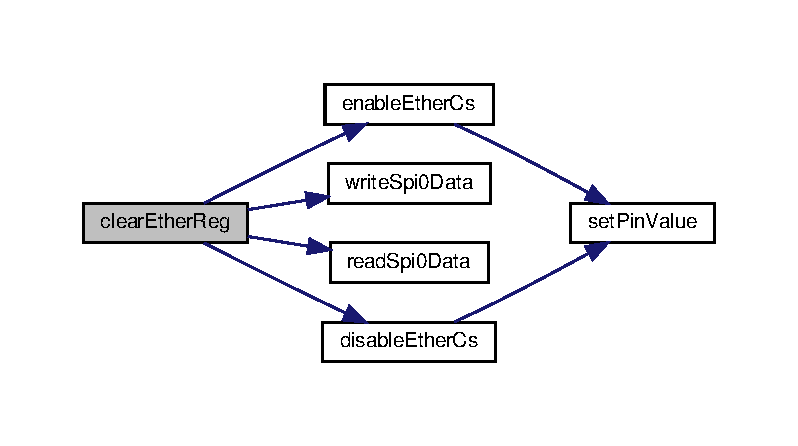
\includegraphics[width=350pt]{eth0_8c_a38241c09b42791119c8dbab457febeda_cgraph}
\end{center}
\end{figure}
Here is the caller graph for this function\+:
\nopagebreak
\begin{figure}[H]
\begin{center}
\leavevmode
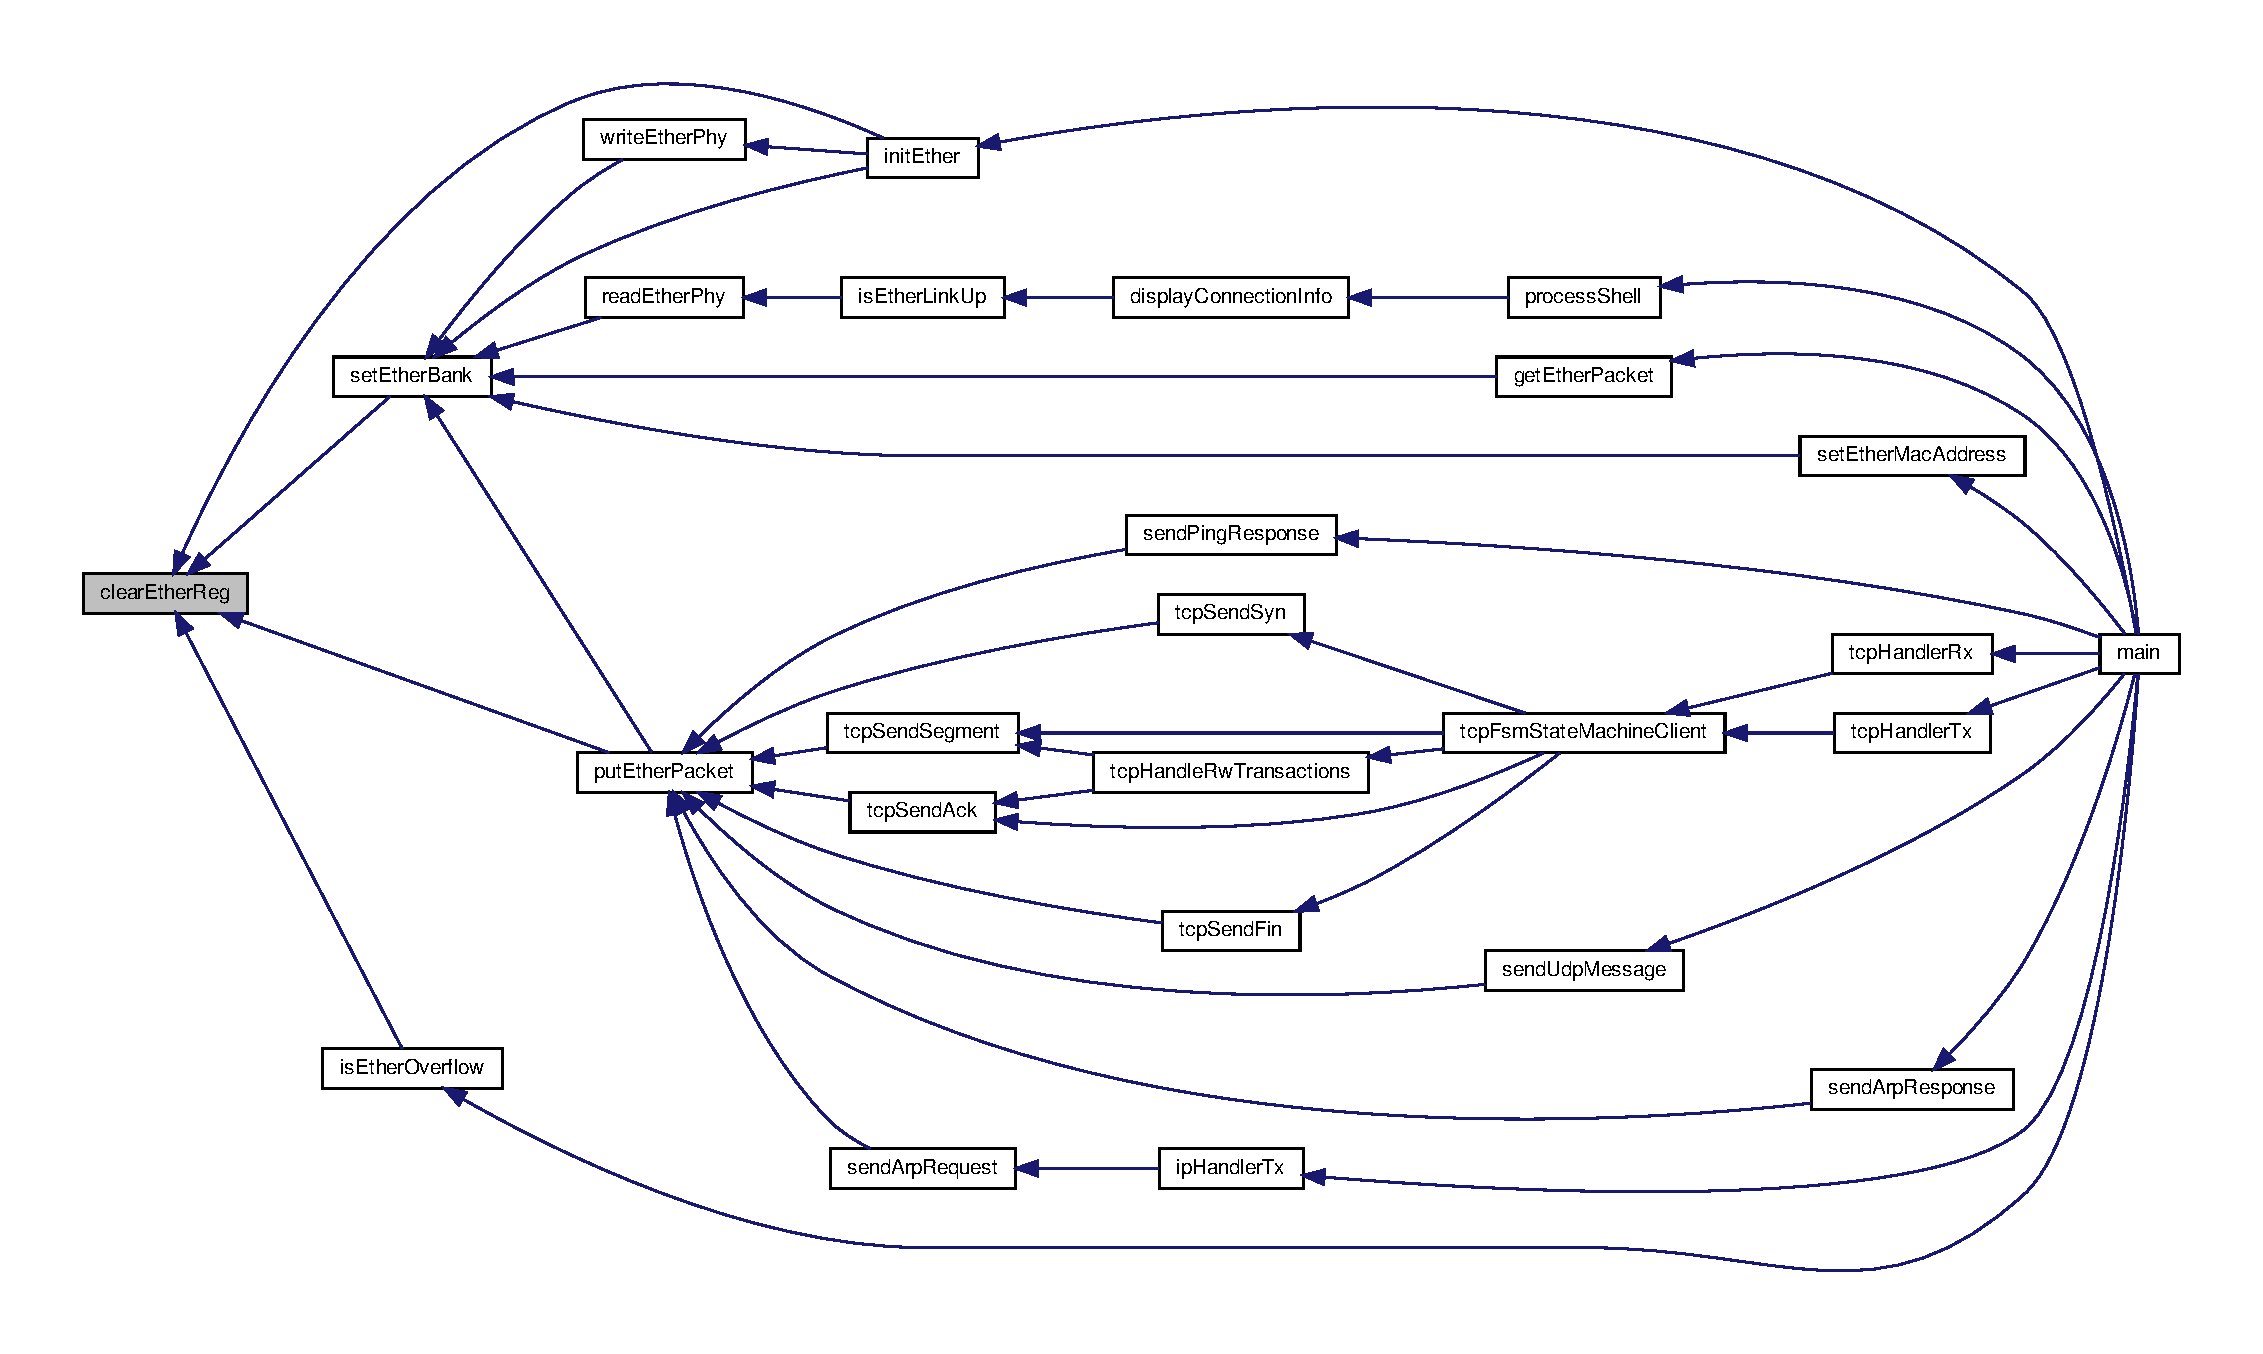
\includegraphics[width=350pt]{eth0_8c_a38241c09b42791119c8dbab457febeda_icgraph}
\end{center}
\end{figure}
\mbox{\Hypertarget{eth0_8c_a159404cc749fadcacda50a180a5adbd7}\label{eth0_8c_a159404cc749fadcacda50a180a5adbd7}} 
\index{eth0.\+c@{eth0.\+c}!disable\+Ether\+Cs@{disable\+Ether\+Cs}}
\index{disable\+Ether\+Cs@{disable\+Ether\+Cs}!eth0.\+c@{eth0.\+c}}
\subsubsection{\texorpdfstring{disable\+Ether\+Cs()}{disableEtherCs()}}
{\footnotesize\ttfamily void disable\+Ether\+Cs (\begin{DoxyParamCaption}\item[{void}]{ }\end{DoxyParamCaption})}



Definition at line 143 of file eth0.\+c.

Here is the call graph for this function\+:
\nopagebreak
\begin{figure}[H]
\begin{center}
\leavevmode
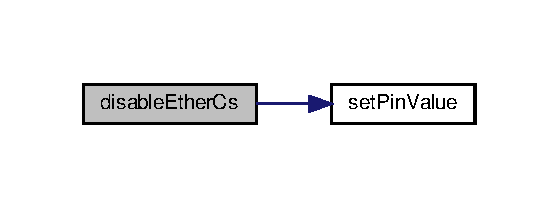
\includegraphics[width=268pt]{eth0_8c_a159404cc749fadcacda50a180a5adbd7_cgraph}
\end{center}
\end{figure}
Here is the caller graph for this function\+:
\nopagebreak
\begin{figure}[H]
\begin{center}
\leavevmode
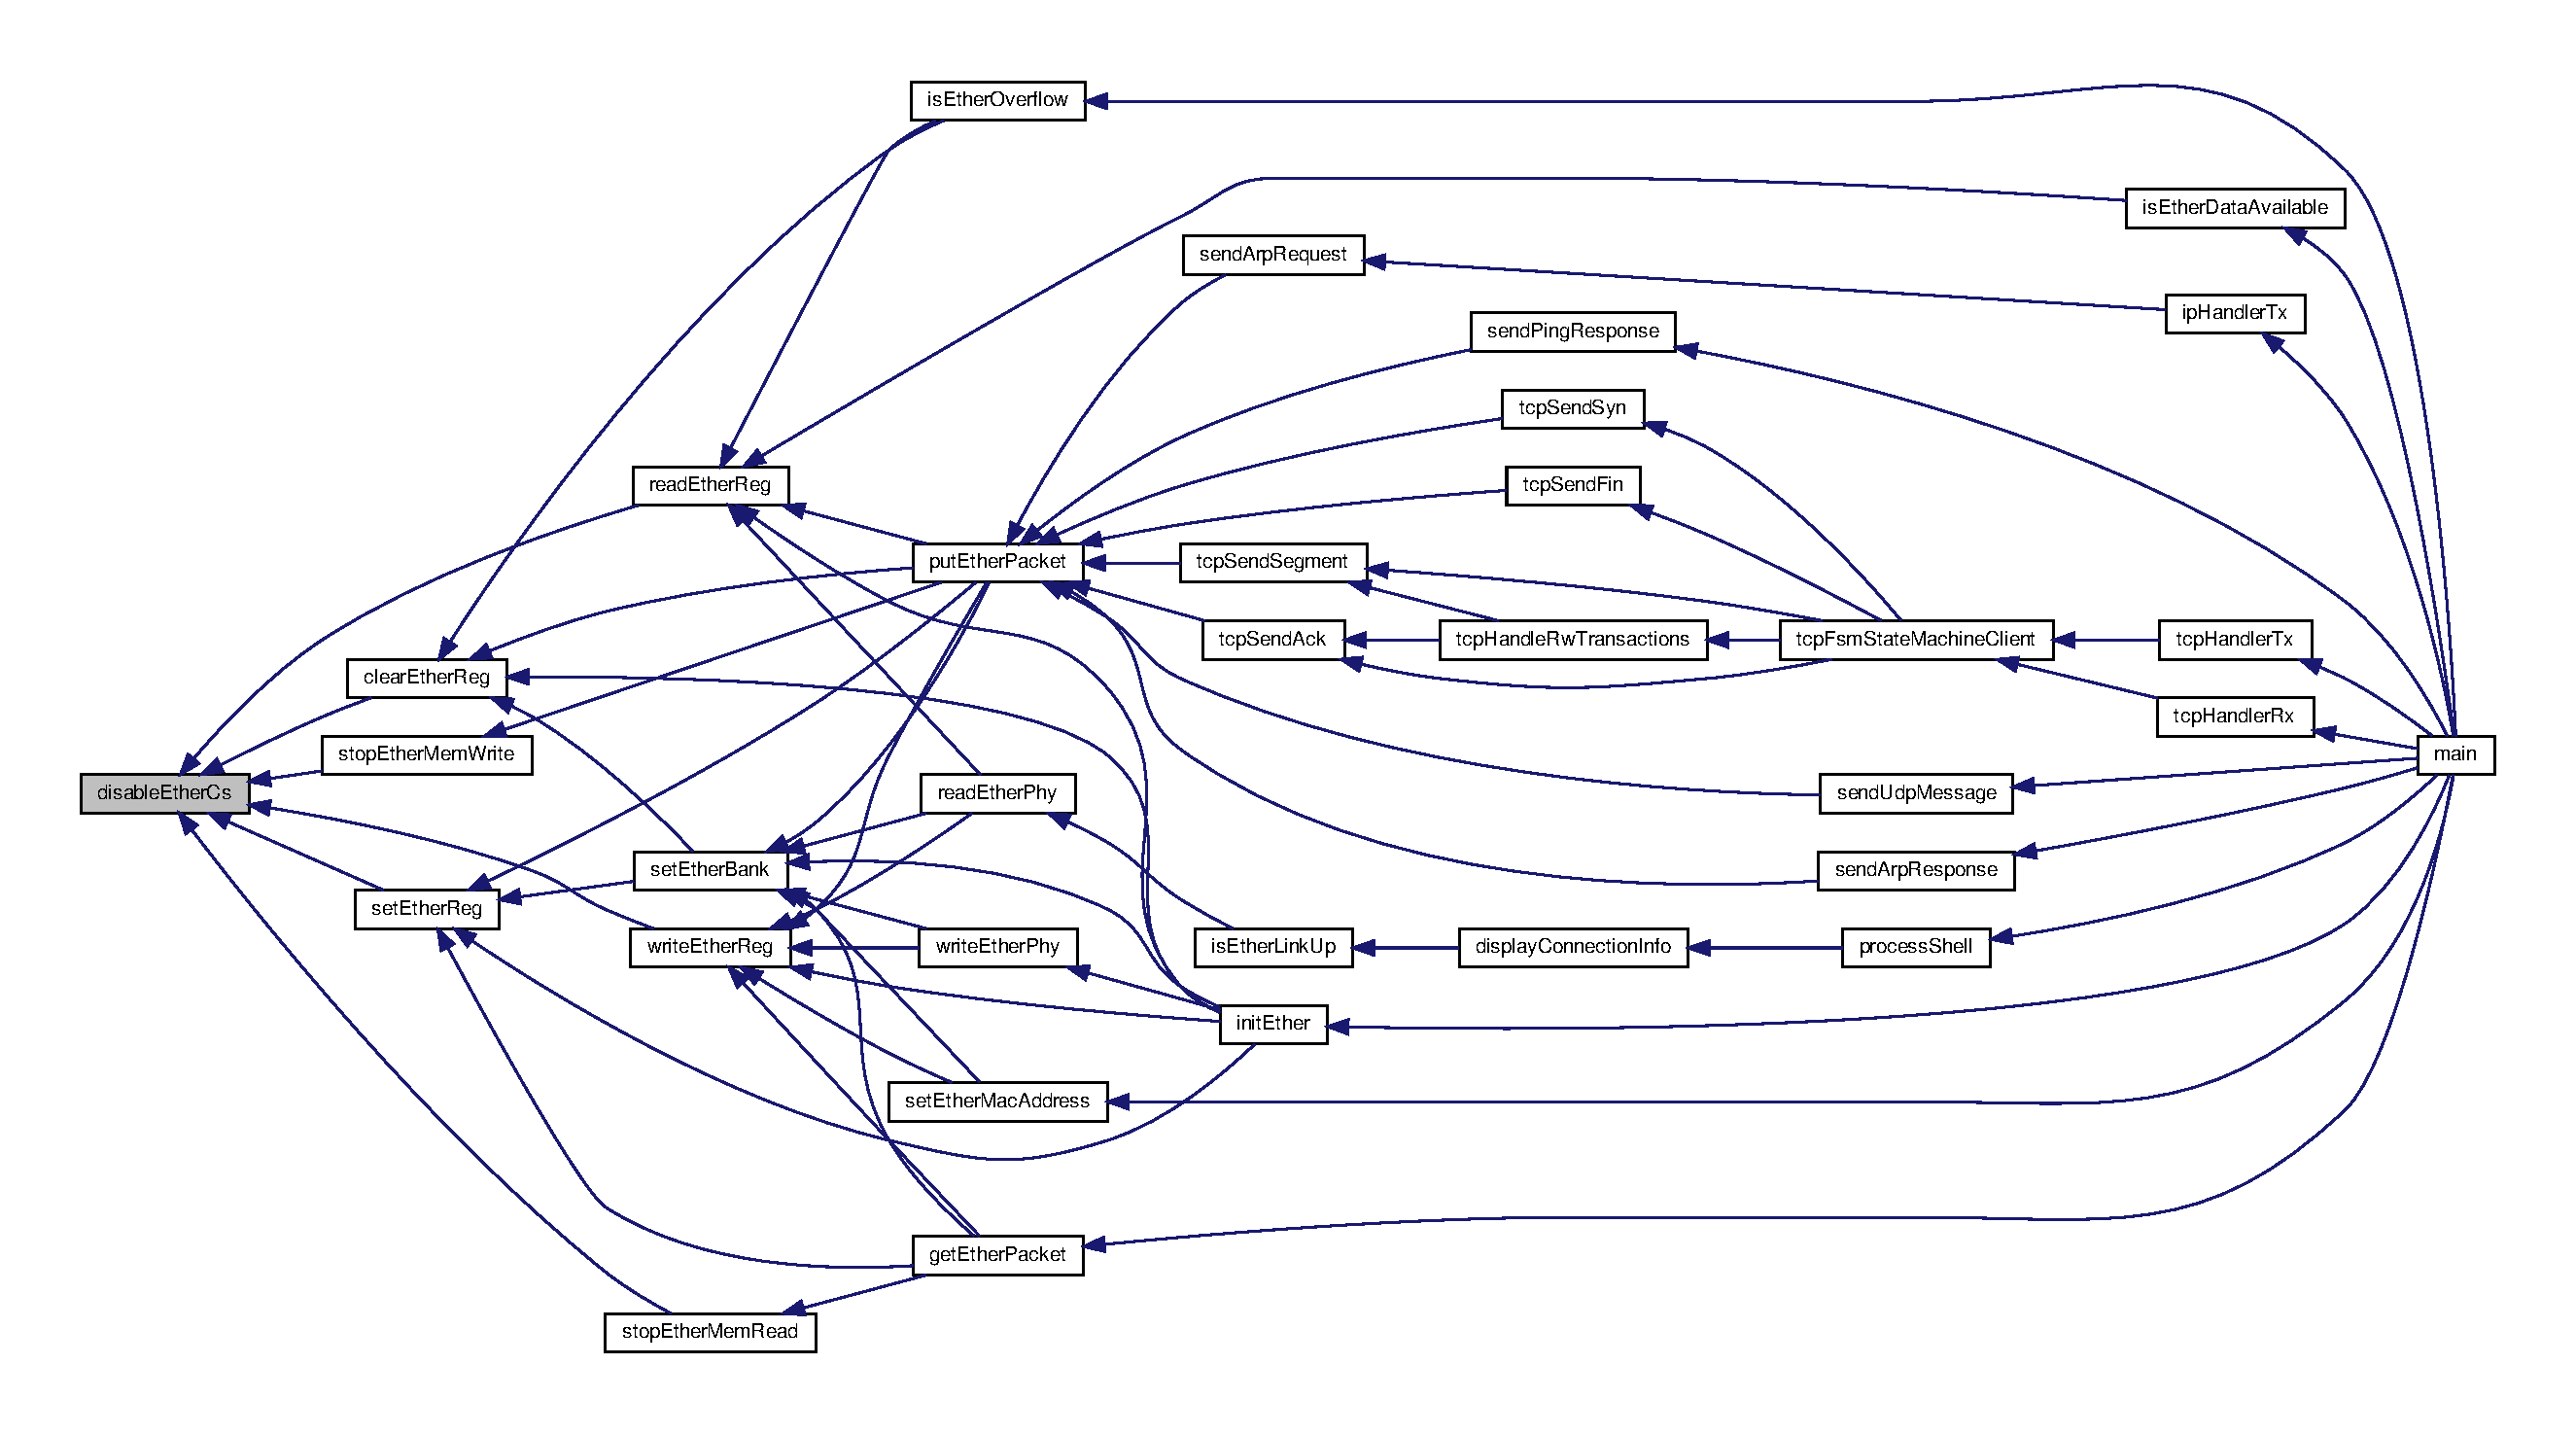
\includegraphics[width=350pt]{eth0_8c_a159404cc749fadcacda50a180a5adbd7_icgraph}
\end{center}
\end{figure}
\mbox{\Hypertarget{eth0_8c_a710f2a378c0c955c211f9e4670ade7ed}\label{eth0_8c_a710f2a378c0c955c211f9e4670ade7ed}} 
\index{eth0.\+c@{eth0.\+c}!enable\+Ether\+Cs@{enable\+Ether\+Cs}}
\index{enable\+Ether\+Cs@{enable\+Ether\+Cs}!eth0.\+c@{eth0.\+c}}
\subsubsection{\texorpdfstring{enable\+Ether\+Cs()}{enableEtherCs()}}
{\footnotesize\ttfamily void enable\+Ether\+Cs (\begin{DoxyParamCaption}\item[{void}]{ }\end{DoxyParamCaption})}



Definition at line 137 of file eth0.\+c.

Here is the call graph for this function\+:
\nopagebreak
\begin{figure}[H]
\begin{center}
\leavevmode
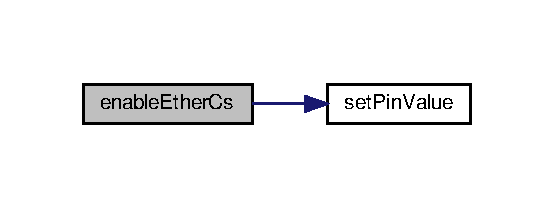
\includegraphics[width=266pt]{eth0_8c_a710f2a378c0c955c211f9e4670ade7ed_cgraph}
\end{center}
\end{figure}
Here is the caller graph for this function\+:
\nopagebreak
\begin{figure}[H]
\begin{center}
\leavevmode
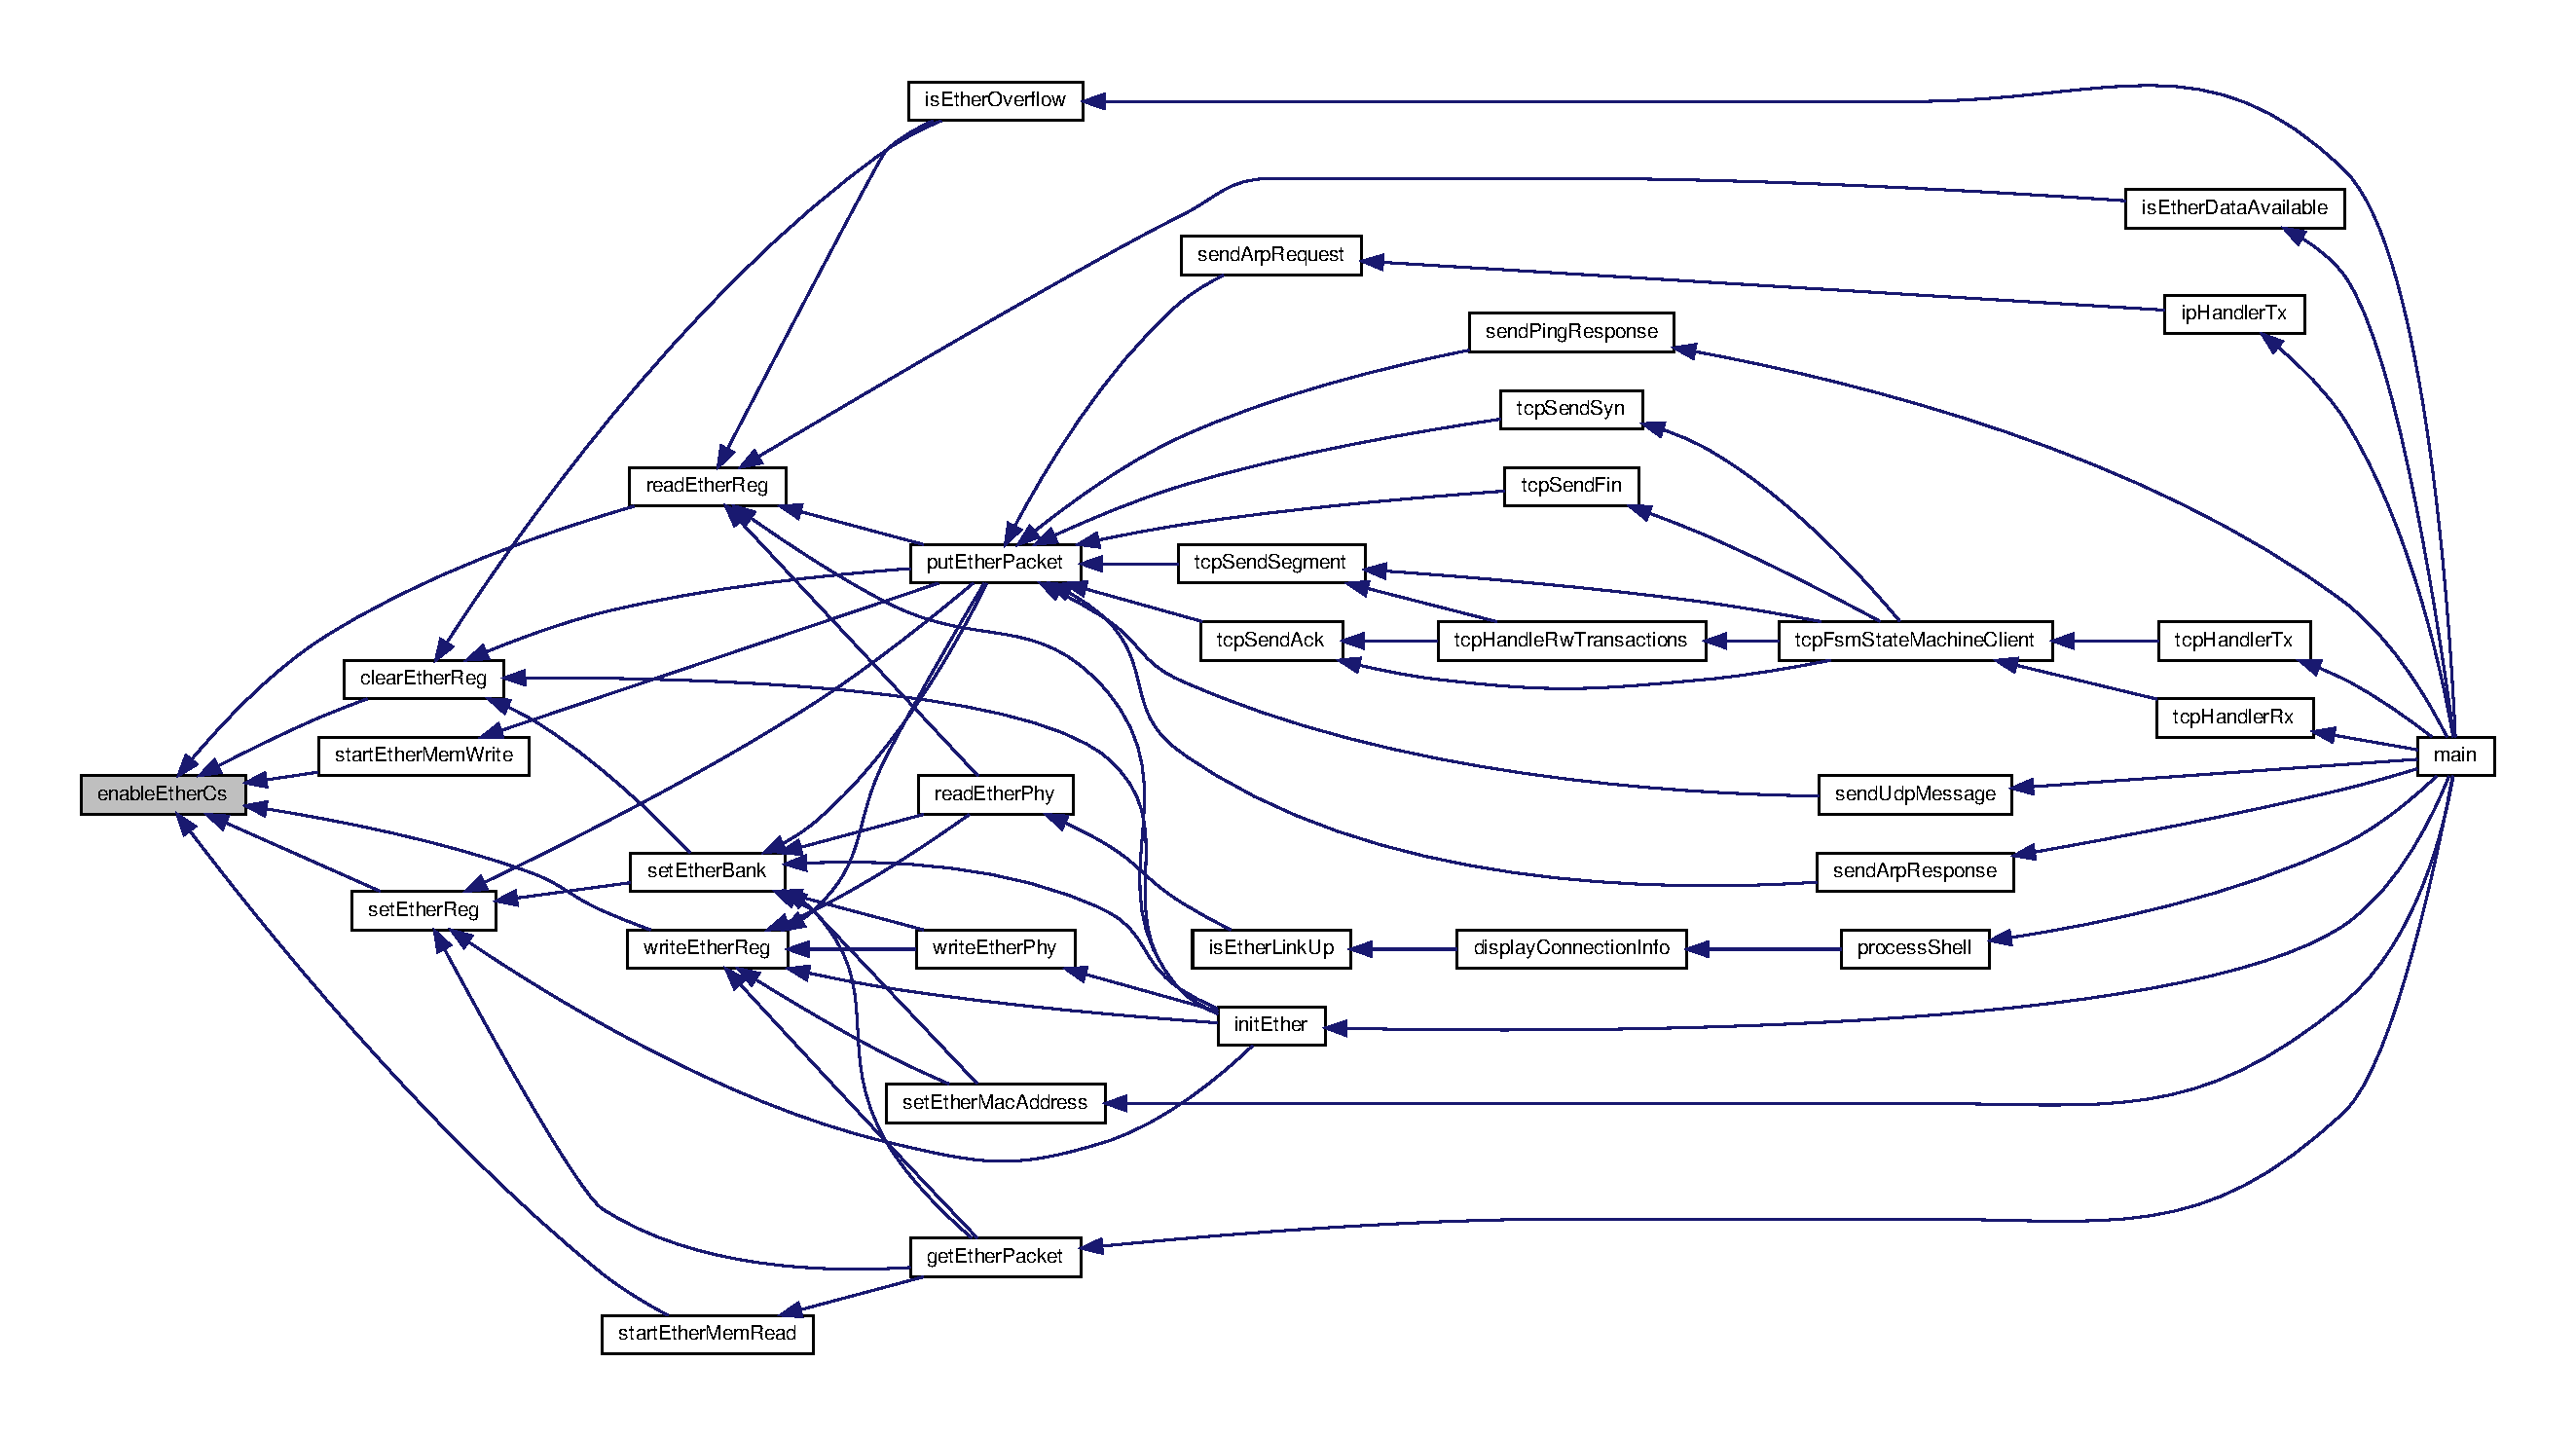
\includegraphics[width=350pt]{eth0_8c_a710f2a378c0c955c211f9e4670ade7ed_icgraph}
\end{center}
\end{figure}
\mbox{\Hypertarget{eth0_8c_a8faf425b2ef6ee8b0d0634e656e45139}\label{eth0_8c_a8faf425b2ef6ee8b0d0634e656e45139}} 
\index{eth0.\+c@{eth0.\+c}!get\+Ether\+Id@{get\+Ether\+Id}}
\index{get\+Ether\+Id@{get\+Ether\+Id}!eth0.\+c@{eth0.\+c}}
\subsubsection{\texorpdfstring{get\+Ether\+Id()}{getEtherId()}}
{\footnotesize\ttfamily uint16\+\_\+t get\+Ether\+Id (\begin{DoxyParamCaption}\item[{void}]{ }\end{DoxyParamCaption})}



Definition at line 486 of file eth0.\+c.

Here is the call graph for this function\+:
\nopagebreak
\begin{figure}[H]
\begin{center}
\leavevmode
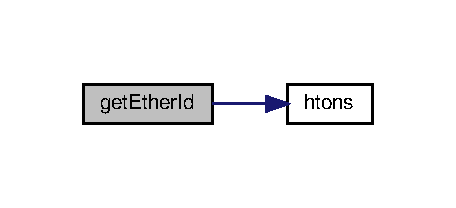
\includegraphics[width=219pt]{eth0_8c_a8faf425b2ef6ee8b0d0634e656e45139_cgraph}
\end{center}
\end{figure}
\mbox{\Hypertarget{eth0_8c_a2310c30c40c60e9f61edbc0c9509c65e}\label{eth0_8c_a2310c30c40c60e9f61edbc0c9509c65e}} 
\index{eth0.\+c@{eth0.\+c}!get\+Ether\+Mac\+Address@{get\+Ether\+Mac\+Address}}
\index{get\+Ether\+Mac\+Address@{get\+Ether\+Mac\+Address}!eth0.\+c@{eth0.\+c}}
\subsubsection{\texorpdfstring{get\+Ether\+Mac\+Address()}{getEtherMacAddress()}}
{\footnotesize\ttfamily void get\+Ether\+Mac\+Address (\begin{DoxyParamCaption}\item[{uint8\+\_\+t}]{mac\mbox{[}\+H\+W\+\_\+\+A\+D\+D\+\_\+\+L\+E\+N\+G\+T\+H\mbox{]} }\end{DoxyParamCaption})}



Definition at line 515 of file eth0.\+c.

Here is the caller graph for this function\+:
\nopagebreak
\begin{figure}[H]
\begin{center}
\leavevmode
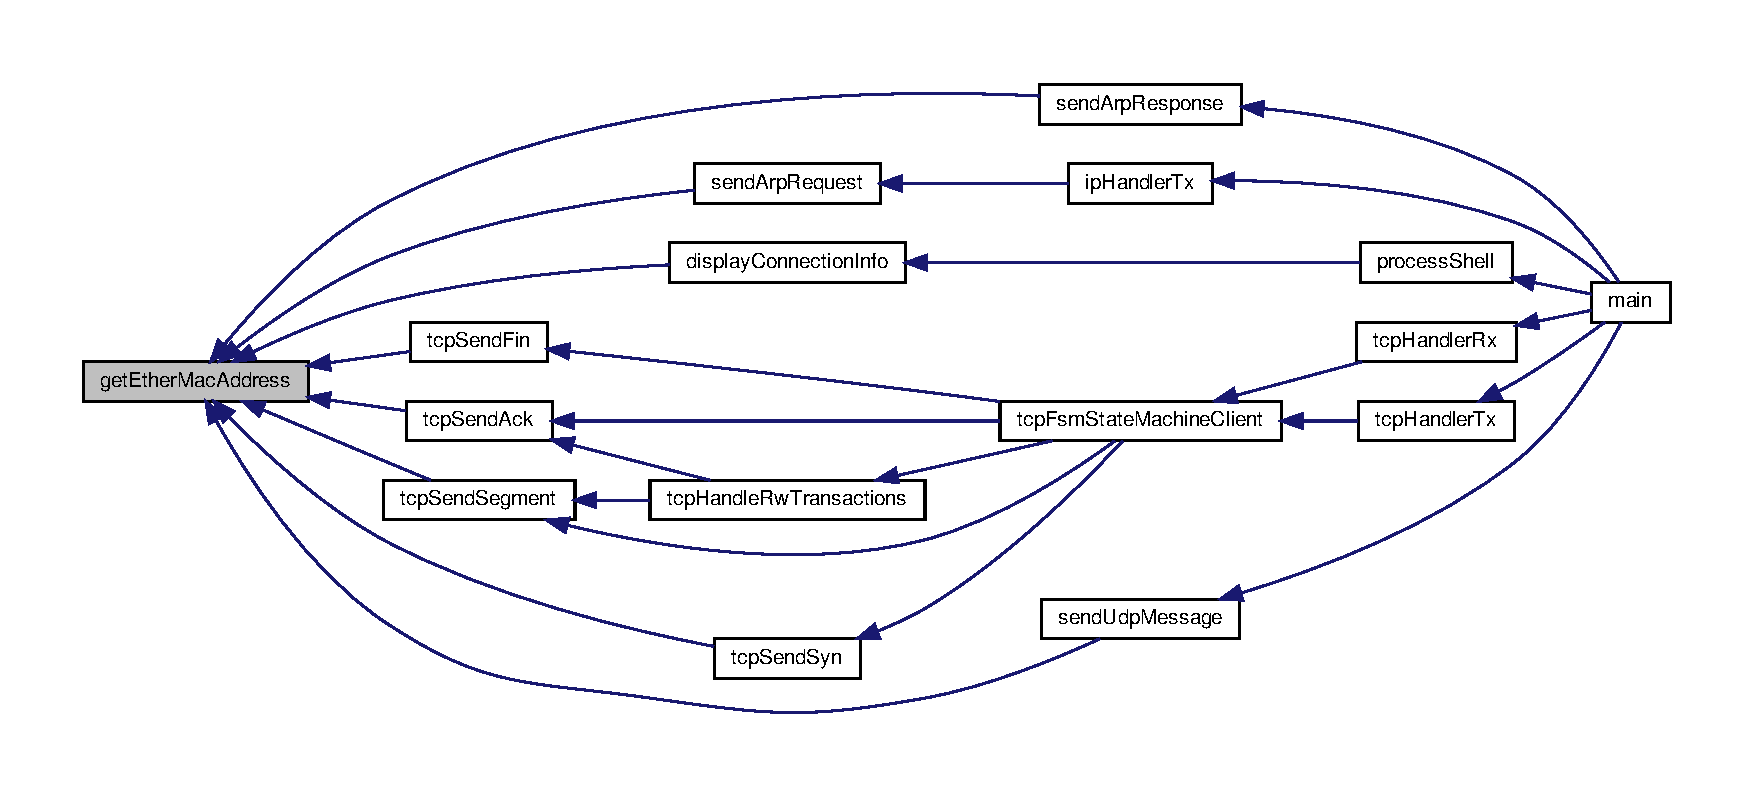
\includegraphics[width=350pt]{eth0_8c_a2310c30c40c60e9f61edbc0c9509c65e_icgraph}
\end{center}
\end{figure}
\mbox{\Hypertarget{eth0_8c_a3c910947910e057b2307632295be61de}\label{eth0_8c_a3c910947910e057b2307632295be61de}} 
\index{eth0.\+c@{eth0.\+c}!get\+Ether\+Packet@{get\+Ether\+Packet}}
\index{get\+Ether\+Packet@{get\+Ether\+Packet}!eth0.\+c@{eth0.\+c}}
\subsubsection{\texorpdfstring{get\+Ether\+Packet()}{getEtherPacket()}}
{\footnotesize\ttfamily uint16\+\_\+t get\+Ether\+Packet (\begin{DoxyParamCaption}\item[{\hyperlink{eth0_8h_a592bdc9f1e029368efe61c7eab510635}{ether\+Header} $\ast$}]{ether,  }\item[{uint16\+\_\+t}]{max\+Size }\end{DoxyParamCaption})}



Definition at line 382 of file eth0.\+c.

Here is the call graph for this function\+:
\nopagebreak
\begin{figure}[H]
\begin{center}
\leavevmode
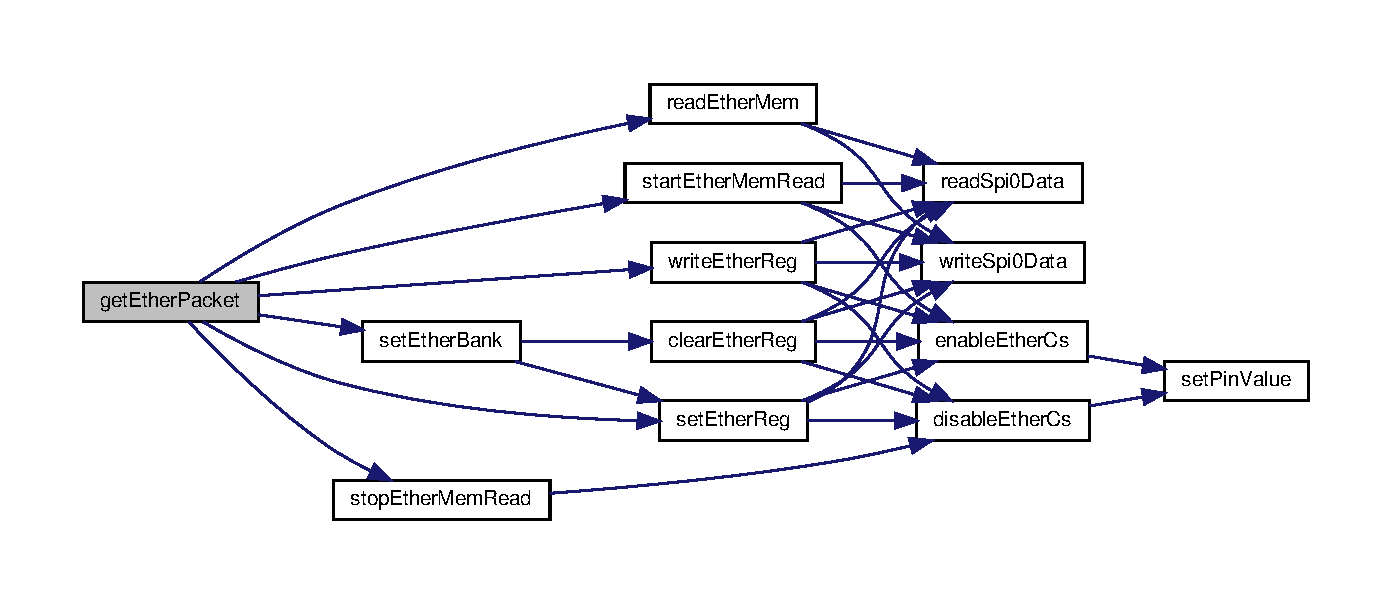
\includegraphics[width=350pt]{eth0_8c_a3c910947910e057b2307632295be61de_cgraph}
\end{center}
\end{figure}
Here is the caller graph for this function\+:
\nopagebreak
\begin{figure}[H]
\begin{center}
\leavevmode
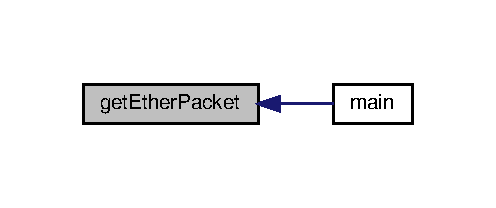
\includegraphics[width=238pt]{eth0_8c_a3c910947910e057b2307632295be61de_icgraph}
\end{center}
\end{figure}
\mbox{\Hypertarget{eth0_8c_a0e7477edd2a29331acedcd4f1d8b0d1a}\label{eth0_8c_a0e7477edd2a29331acedcd4f1d8b0d1a}} 
\index{eth0.\+c@{eth0.\+c}!htonl@{htonl}}
\index{htonl@{htonl}!eth0.\+c@{eth0.\+c}}
\subsubsection{\texorpdfstring{htonl()}{htonl()}}
{\footnotesize\ttfamily uint32\+\_\+t htonl (\begin{DoxyParamCaption}\item[{uint32\+\_\+t}]{value }\end{DoxyParamCaption})}



Definition at line 480 of file eth0.\+c.

Here is the caller graph for this function\+:
\nopagebreak
\begin{figure}[H]
\begin{center}
\leavevmode
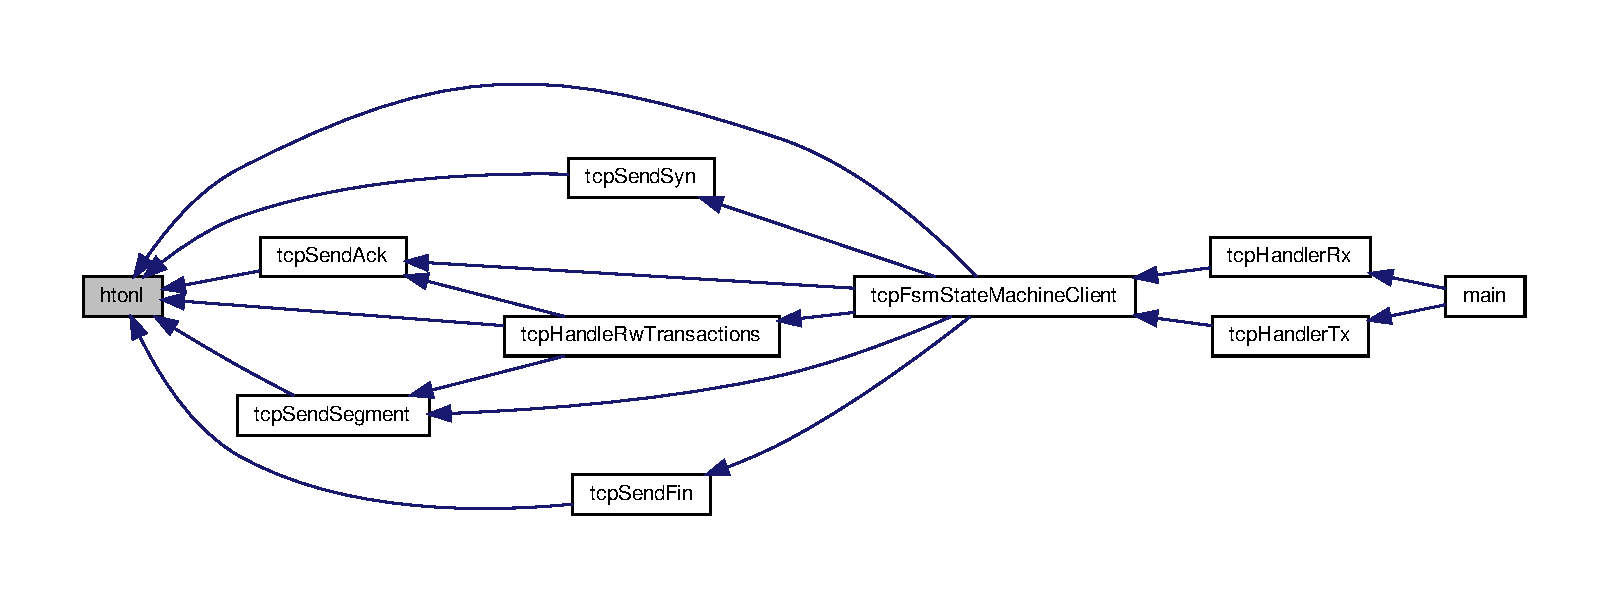
\includegraphics[width=350pt]{eth0_8c_a0e7477edd2a29331acedcd4f1d8b0d1a_icgraph}
\end{center}
\end{figure}
\mbox{\Hypertarget{eth0_8c_af86d9622798ed7e76bd7de347df940ae}\label{eth0_8c_af86d9622798ed7e76bd7de347df940ae}} 
\index{eth0.\+c@{eth0.\+c}!htons@{htons}}
\index{htons@{htons}!eth0.\+c@{eth0.\+c}}
\subsubsection{\texorpdfstring{htons()}{htons()}}
{\footnotesize\ttfamily uint16\+\_\+t htons (\begin{DoxyParamCaption}\item[{uint16\+\_\+t}]{value }\end{DoxyParamCaption})}



Definition at line 475 of file eth0.\+c.

Here is the caller graph for this function\+:
\nopagebreak
\begin{figure}[H]
\begin{center}
\leavevmode
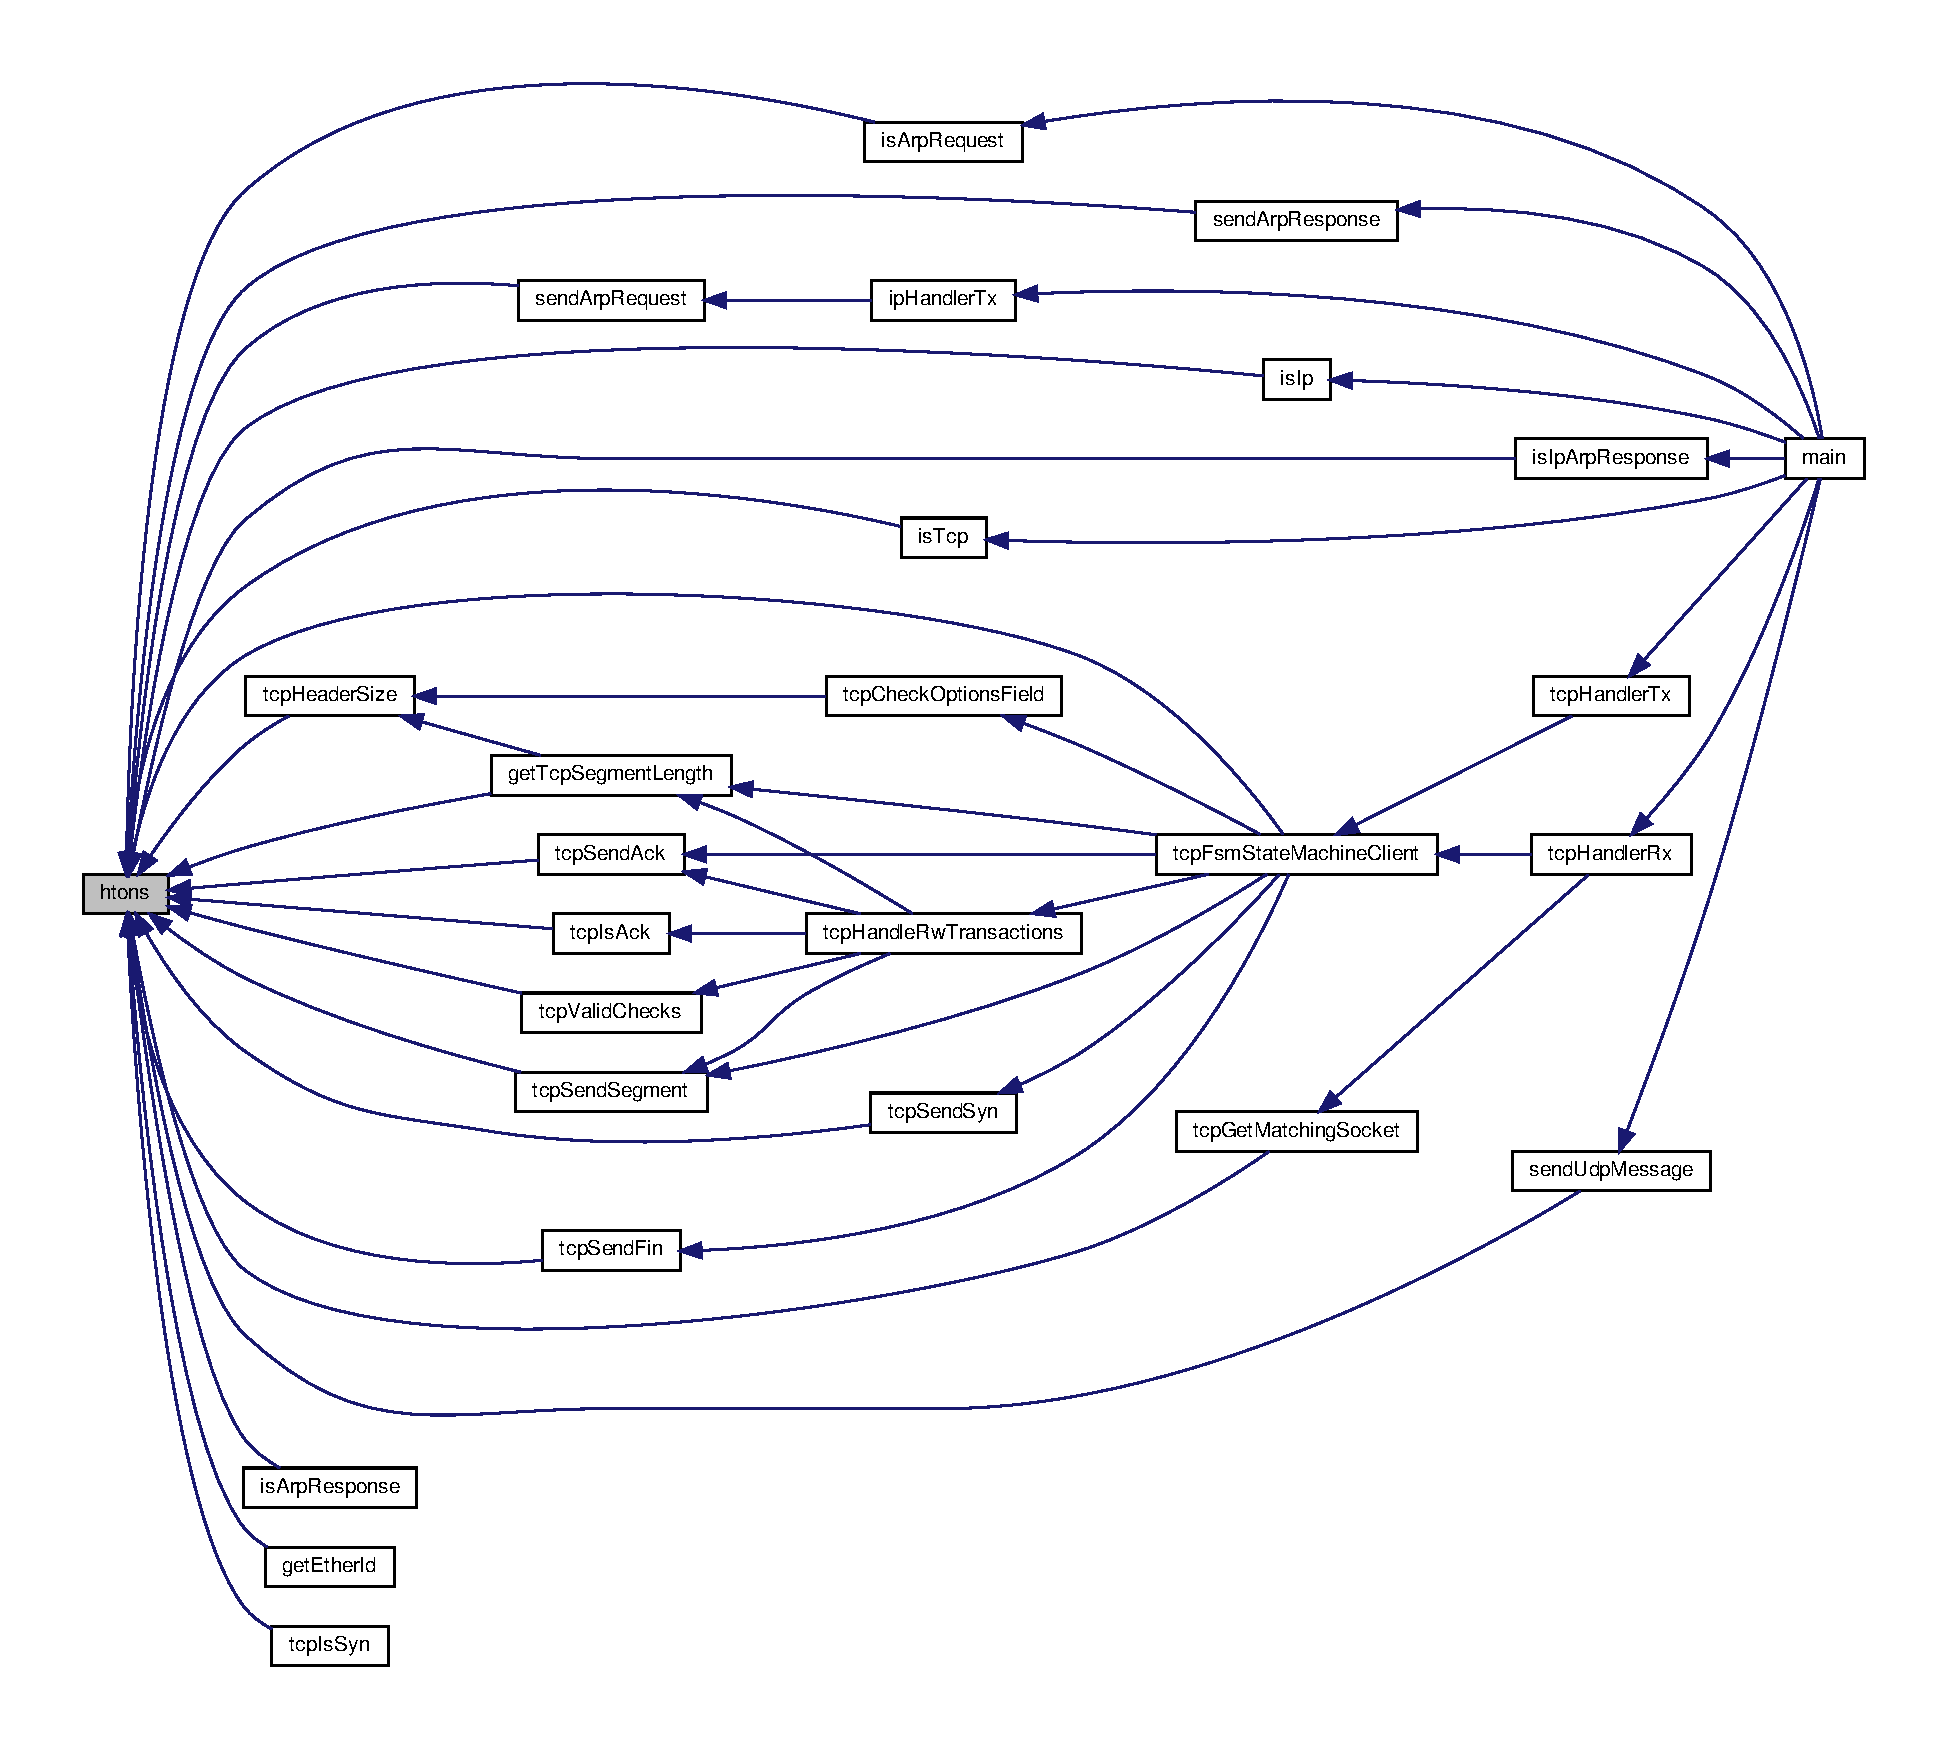
\includegraphics[width=350pt]{eth0_8c_af86d9622798ed7e76bd7de347df940ae_icgraph}
\end{center}
\end{figure}
\mbox{\Hypertarget{eth0_8c_aafe022cdee56a8cfeb19b3a40d1ff768}\label{eth0_8c_aafe022cdee56a8cfeb19b3a40d1ff768}} 
\index{eth0.\+c@{eth0.\+c}!inc\+Ether\+Id@{inc\+Ether\+Id}}
\index{inc\+Ether\+Id@{inc\+Ether\+Id}!eth0.\+c@{eth0.\+c}}
\subsubsection{\texorpdfstring{inc\+Ether\+Id()}{incEtherId()}}
{\footnotesize\ttfamily void inc\+Ether\+Id (\begin{DoxyParamCaption}\item[{void}]{ }\end{DoxyParamCaption})}



Definition at line 491 of file eth0.\+c.

\mbox{\Hypertarget{eth0_8c_aecae72b4579b409c7c7c90c2c12237f1}\label{eth0_8c_aecae72b4579b409c7c7c90c2c12237f1}} 
\index{eth0.\+c@{eth0.\+c}!init\+Ether@{init\+Ether}}
\index{init\+Ether@{init\+Ether}!eth0.\+c@{eth0.\+c}}
\subsubsection{\texorpdfstring{init\+Ether()}{initEther()}}
{\footnotesize\ttfamily void init\+Ether (\begin{DoxyParamCaption}\item[{uint16\+\_\+t}]{mode }\end{DoxyParamCaption})}



Definition at line 259 of file eth0.\+c.

Here is the call graph for this function\+:
\nopagebreak
\begin{figure}[H]
\begin{center}
\leavevmode
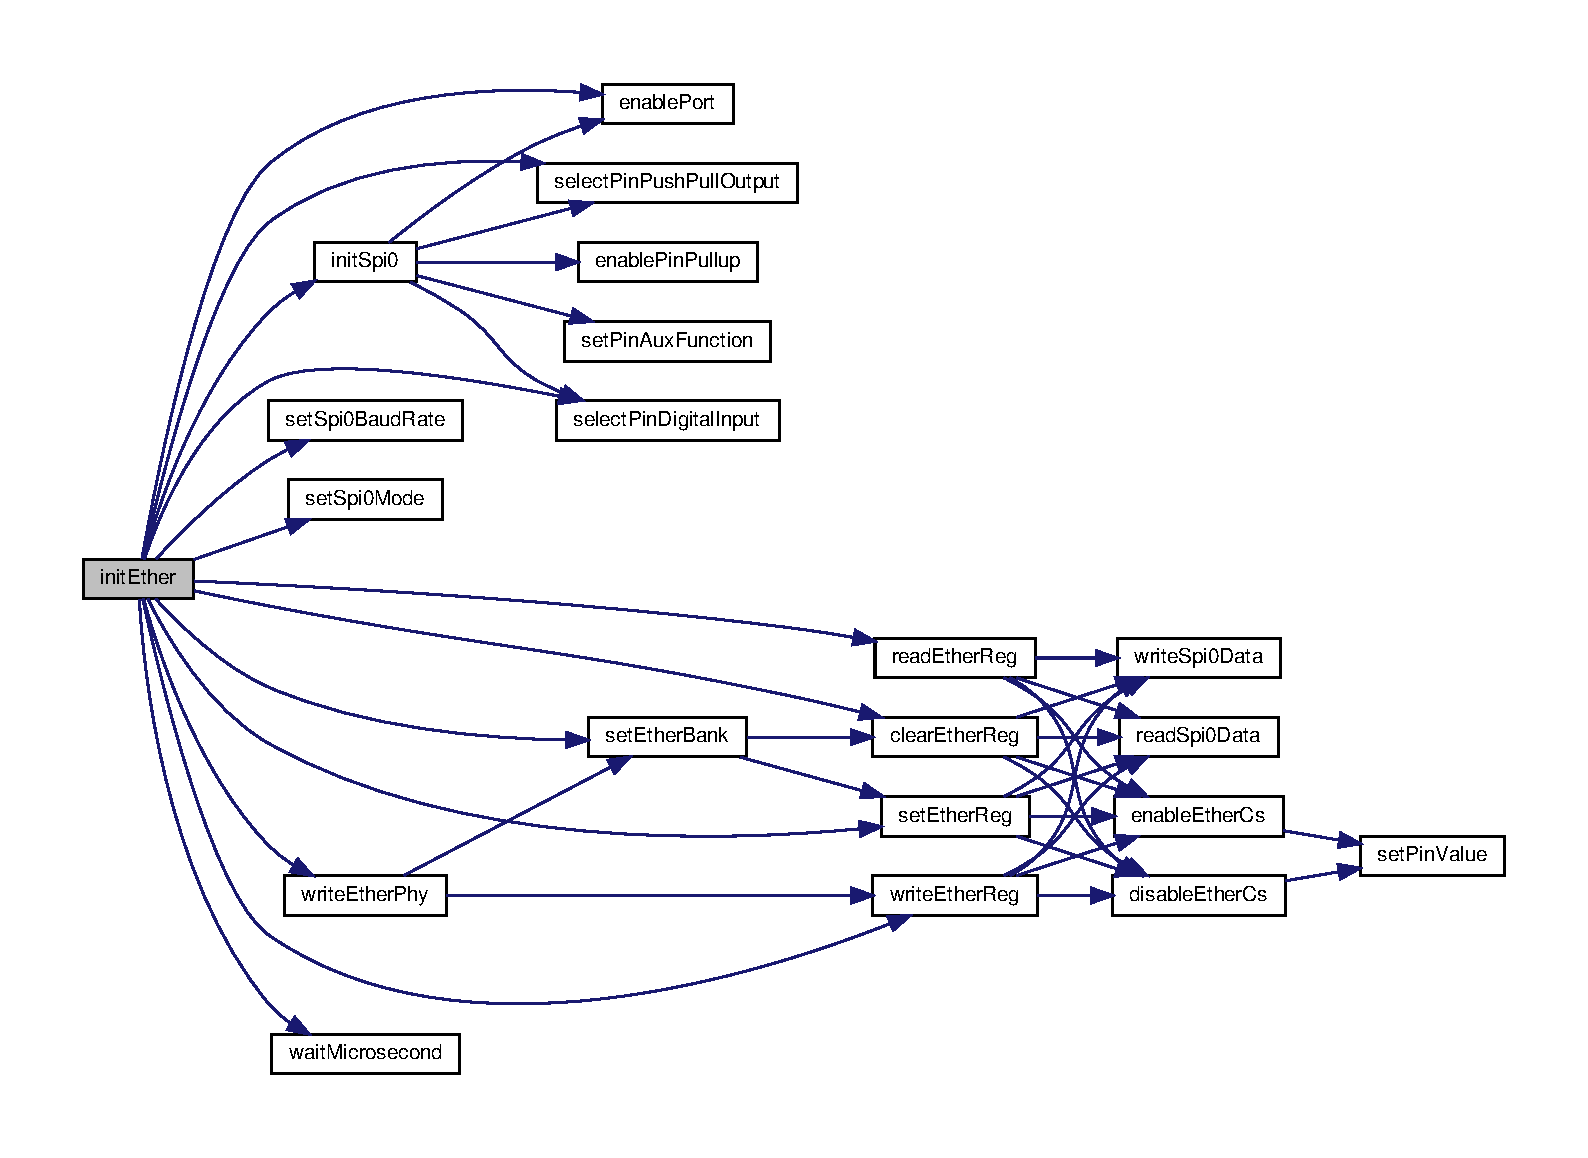
\includegraphics[width=350pt]{eth0_8c_aecae72b4579b409c7c7c90c2c12237f1_cgraph}
\end{center}
\end{figure}
Here is the caller graph for this function\+:
\nopagebreak
\begin{figure}[H]
\begin{center}
\leavevmode
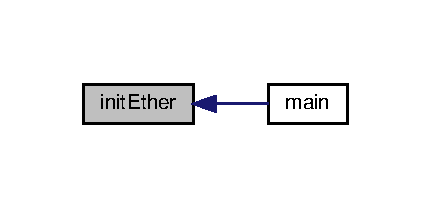
\includegraphics[width=207pt]{eth0_8c_aecae72b4579b409c7c7c90c2c12237f1_icgraph}
\end{center}
\end{figure}
\mbox{\Hypertarget{eth0_8c_abbc16de0f8318b921e173fdea69650f0}\label{eth0_8c_abbc16de0f8318b921e173fdea69650f0}} 
\index{eth0.\+c@{eth0.\+c}!is\+Ether\+Data\+Available@{is\+Ether\+Data\+Available}}
\index{is\+Ether\+Data\+Available@{is\+Ether\+Data\+Available}!eth0.\+c@{eth0.\+c}}
\subsubsection{\texorpdfstring{is\+Ether\+Data\+Available()}{isEtherDataAvailable()}}
{\footnotesize\ttfamily bool is\+Ether\+Data\+Available (\begin{DoxyParamCaption}\item[{void}]{ }\end{DoxyParamCaption})}



Definition at line 364 of file eth0.\+c.

Here is the call graph for this function\+:
\nopagebreak
\begin{figure}[H]
\begin{center}
\leavevmode
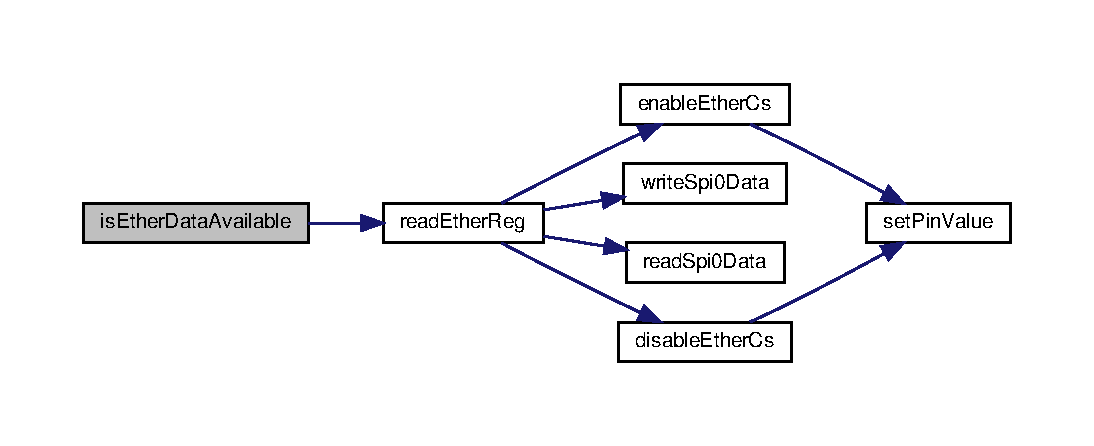
\includegraphics[width=350pt]{eth0_8c_abbc16de0f8318b921e173fdea69650f0_cgraph}
\end{center}
\end{figure}
Here is the caller graph for this function\+:
\nopagebreak
\begin{figure}[H]
\begin{center}
\leavevmode
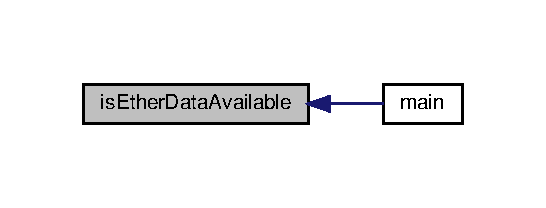
\includegraphics[width=262pt]{eth0_8c_abbc16de0f8318b921e173fdea69650f0_icgraph}
\end{center}
\end{figure}
\mbox{\Hypertarget{eth0_8c_a3bbcc2a0d14181ed2dc3f1e221997ee5}\label{eth0_8c_a3bbcc2a0d14181ed2dc3f1e221997ee5}} 
\index{eth0.\+c@{eth0.\+c}!is\+Ether\+Link\+Up@{is\+Ether\+Link\+Up}}
\index{is\+Ether\+Link\+Up@{is\+Ether\+Link\+Up}!eth0.\+c@{eth0.\+c}}
\subsubsection{\texorpdfstring{is\+Ether\+Link\+Up()}{isEtherLinkUp()}}
{\footnotesize\ttfamily bool is\+Ether\+Link\+Up (\begin{DoxyParamCaption}\item[{void}]{ }\end{DoxyParamCaption})}



Definition at line 358 of file eth0.\+c.

Here is the call graph for this function\+:
\nopagebreak
\begin{figure}[H]
\begin{center}
\leavevmode
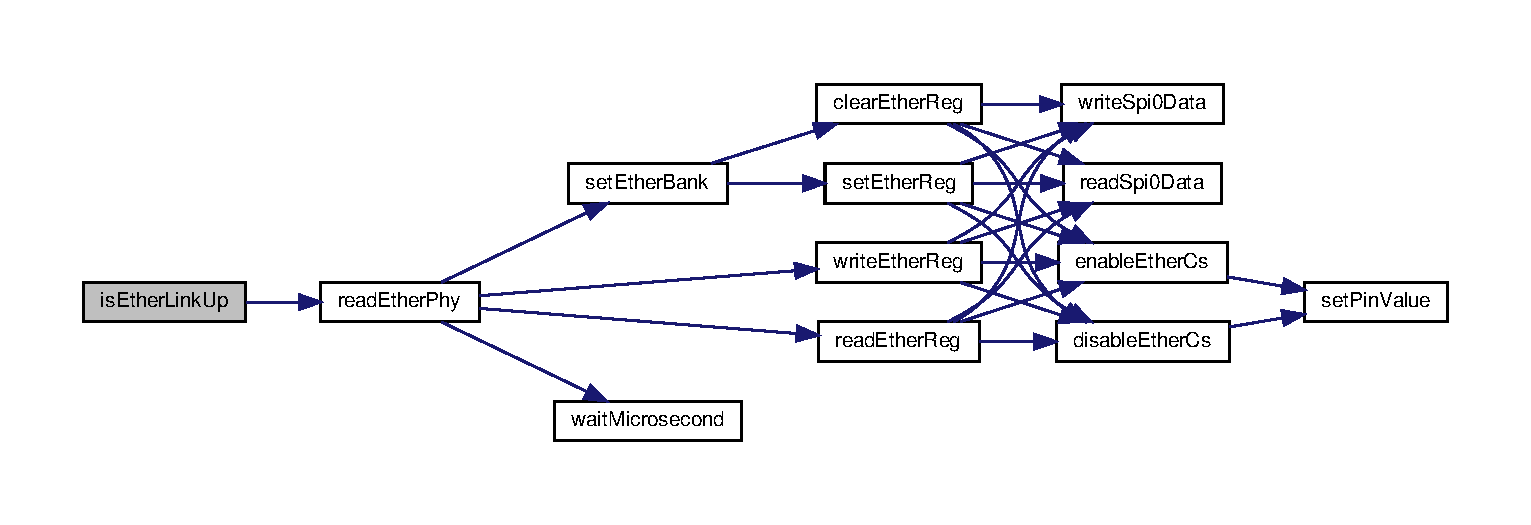
\includegraphics[width=350pt]{eth0_8c_a3bbcc2a0d14181ed2dc3f1e221997ee5_cgraph}
\end{center}
\end{figure}
Here is the caller graph for this function\+:
\nopagebreak
\begin{figure}[H]
\begin{center}
\leavevmode
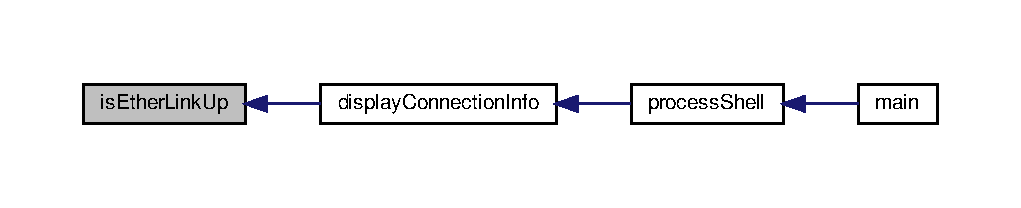
\includegraphics[width=350pt]{eth0_8c_a3bbcc2a0d14181ed2dc3f1e221997ee5_icgraph}
\end{center}
\end{figure}
\mbox{\Hypertarget{eth0_8c_a0ca653f48ca731d0be8fcb8af85c54bf}\label{eth0_8c_a0ca653f48ca731d0be8fcb8af85c54bf}} 
\index{eth0.\+c@{eth0.\+c}!is\+Ether\+Overflow@{is\+Ether\+Overflow}}
\index{is\+Ether\+Overflow@{is\+Ether\+Overflow}!eth0.\+c@{eth0.\+c}}
\subsubsection{\texorpdfstring{is\+Ether\+Overflow()}{isEtherOverflow()}}
{\footnotesize\ttfamily bool is\+Ether\+Overflow (\begin{DoxyParamCaption}\item[{void}]{ }\end{DoxyParamCaption})}



Definition at line 370 of file eth0.\+c.

Here is the call graph for this function\+:
\nopagebreak
\begin{figure}[H]
\begin{center}
\leavevmode
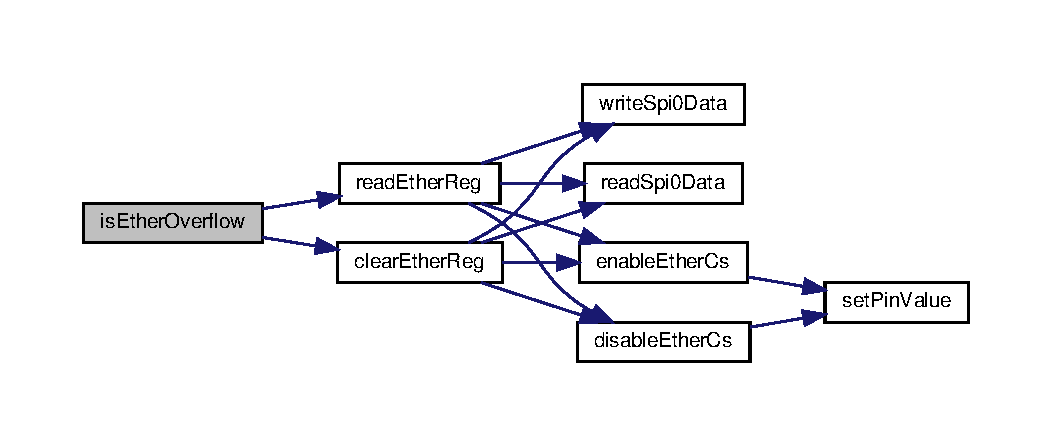
\includegraphics[width=350pt]{eth0_8c_a0ca653f48ca731d0be8fcb8af85c54bf_cgraph}
\end{center}
\end{figure}
Here is the caller graph for this function\+:
\nopagebreak
\begin{figure}[H]
\begin{center}
\leavevmode
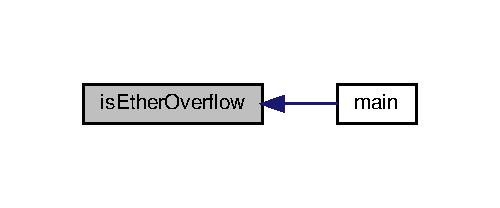
\includegraphics[width=240pt]{eth0_8c_a0ca653f48ca731d0be8fcb8af85c54bf_icgraph}
\end{center}
\end{figure}
\mbox{\Hypertarget{eth0_8c_a9908befa3f95ad0b652ef68a53000634}\label{eth0_8c_a9908befa3f95ad0b652ef68a53000634}} 
\index{eth0.\+c@{eth0.\+c}!put\+Ether\+Packet@{put\+Ether\+Packet}}
\index{put\+Ether\+Packet@{put\+Ether\+Packet}!eth0.\+c@{eth0.\+c}}
\subsubsection{\texorpdfstring{put\+Ether\+Packet()}{putEtherPacket()}}
{\footnotesize\ttfamily bool put\+Ether\+Packet (\begin{DoxyParamCaption}\item[{\hyperlink{eth0_8h_a592bdc9f1e029368efe61c7eab510635}{ether\+Header} $\ast$}]{ether,  }\item[{uint16\+\_\+t}]{size }\end{DoxyParamCaption})}



Definition at line 428 of file eth0.\+c.

Here is the call graph for this function\+:
\nopagebreak
\begin{figure}[H]
\begin{center}
\leavevmode
\includegraphics[width=350pt]{eth0_8c_a9908befa3f95ad0b652ef68a53000634_cgraph}
\end{center}
\end{figure}
Here is the caller graph for this function\+:
\nopagebreak
\begin{figure}[H]
\begin{center}
\leavevmode
\includegraphics[width=350pt]{eth0_8c_a9908befa3f95ad0b652ef68a53000634_icgraph}
\end{center}
\end{figure}
\mbox{\Hypertarget{eth0_8c_aaa4099eb7c6e6b9ef1cc0214e3736c0b}\label{eth0_8c_aaa4099eb7c6e6b9ef1cc0214e3736c0b}} 
\index{eth0.\+c@{eth0.\+c}!read\+Ether\+Mem@{read\+Ether\+Mem}}
\index{read\+Ether\+Mem@{read\+Ether\+Mem}!eth0.\+c@{eth0.\+c}}
\subsubsection{\texorpdfstring{read\+Ether\+Mem()}{readEtherMem()}}
{\footnotesize\ttfamily uint8\+\_\+t read\+Ether\+Mem (\begin{DoxyParamCaption}\item[{void}]{ }\end{DoxyParamCaption})}



Definition at line 246 of file eth0.\+c.

Here is the call graph for this function\+:
\nopagebreak
\begin{figure}[H]
\begin{center}
\leavevmode
\includegraphics[width=274pt]{eth0_8c_aaa4099eb7c6e6b9ef1cc0214e3736c0b_cgraph}
\end{center}
\end{figure}
Here is the caller graph for this function\+:
\nopagebreak
\begin{figure}[H]
\begin{center}
\leavevmode
\includegraphics[width=350pt]{eth0_8c_aaa4099eb7c6e6b9ef1cc0214e3736c0b_icgraph}
\end{center}
\end{figure}
\mbox{\Hypertarget{eth0_8c_a794aa232a607af373be4e2abffb74ef8}\label{eth0_8c_a794aa232a607af373be4e2abffb74ef8}} 
\index{eth0.\+c@{eth0.\+c}!read\+Ether\+Phy@{read\+Ether\+Phy}}
\index{read\+Ether\+Phy@{read\+Ether\+Phy}!eth0.\+c@{eth0.\+c}}
\subsubsection{\texorpdfstring{read\+Ether\+Phy()}{readEtherPhy()}}
{\footnotesize\ttfamily uint16\+\_\+t read\+Ether\+Phy (\begin{DoxyParamCaption}\item[{uint8\+\_\+t}]{reg }\end{DoxyParamCaption})}



Definition at line 204 of file eth0.\+c.

Here is the call graph for this function\+:
\nopagebreak
\begin{figure}[H]
\begin{center}
\leavevmode
\includegraphics[width=350pt]{eth0_8c_a794aa232a607af373be4e2abffb74ef8_cgraph}
\end{center}
\end{figure}
Here is the caller graph for this function\+:
\nopagebreak
\begin{figure}[H]
\begin{center}
\leavevmode
\includegraphics[width=350pt]{eth0_8c_a794aa232a607af373be4e2abffb74ef8_icgraph}
\end{center}
\end{figure}
\mbox{\Hypertarget{eth0_8c_aceaa52a49cf227193b6a1b49cfc03d84}\label{eth0_8c_aceaa52a49cf227193b6a1b49cfc03d84}} 
\index{eth0.\+c@{eth0.\+c}!read\+Ether\+Reg@{read\+Ether\+Reg}}
\index{read\+Ether\+Reg@{read\+Ether\+Reg}!eth0.\+c@{eth0.\+c}}
\subsubsection{\texorpdfstring{read\+Ether\+Reg()}{readEtherReg()}}
{\footnotesize\ttfamily uint8\+\_\+t read\+Ether\+Reg (\begin{DoxyParamCaption}\item[{uint8\+\_\+t}]{reg }\end{DoxyParamCaption})}



Definition at line 158 of file eth0.\+c.

Here is the call graph for this function\+:
\nopagebreak
\begin{figure}[H]
\begin{center}
\leavevmode
\includegraphics[width=350pt]{eth0_8c_aceaa52a49cf227193b6a1b49cfc03d84_cgraph}
\end{center}
\end{figure}
Here is the caller graph for this function\+:
\nopagebreak
\begin{figure}[H]
\begin{center}
\leavevmode
\includegraphics[width=350pt]{eth0_8c_aceaa52a49cf227193b6a1b49cfc03d84_icgraph}
\end{center}
\end{figure}
\mbox{\Hypertarget{eth0_8c_ae1db6f1bddfe9bfec4eaff780300f72e}\label{eth0_8c_ae1db6f1bddfe9bfec4eaff780300f72e}} 
\index{eth0.\+c@{eth0.\+c}!set\+Ether\+Bank@{set\+Ether\+Bank}}
\index{set\+Ether\+Bank@{set\+Ether\+Bank}!eth0.\+c@{eth0.\+c}}
\subsubsection{\texorpdfstring{set\+Ether\+Bank()}{setEtherBank()}}
{\footnotesize\ttfamily void set\+Ether\+Bank (\begin{DoxyParamCaption}\item[{uint8\+\_\+t}]{reg }\end{DoxyParamCaption})}



Definition at line 190 of file eth0.\+c.

Here is the call graph for this function\+:
\nopagebreak
\begin{figure}[H]
\begin{center}
\leavevmode
\includegraphics[width=350pt]{eth0_8c_ae1db6f1bddfe9bfec4eaff780300f72e_cgraph}
\end{center}
\end{figure}
Here is the caller graph for this function\+:
\nopagebreak
\begin{figure}[H]
\begin{center}
\leavevmode
\includegraphics[width=350pt]{eth0_8c_ae1db6f1bddfe9bfec4eaff780300f72e_icgraph}
\end{center}
\end{figure}
\mbox{\Hypertarget{eth0_8c_afcc4d6e0bb55eb862abfd8da36d1cd6d}\label{eth0_8c_afcc4d6e0bb55eb862abfd8da36d1cd6d}} 
\index{eth0.\+c@{eth0.\+c}!set\+Ether\+Mac\+Address@{set\+Ether\+Mac\+Address}}
\index{set\+Ether\+Mac\+Address@{set\+Ether\+Mac\+Address}!eth0.\+c@{eth0.\+c}}
\subsubsection{\texorpdfstring{set\+Ether\+Mac\+Address()}{setEtherMacAddress()}}
{\footnotesize\ttfamily void set\+Ether\+Mac\+Address (\begin{DoxyParamCaption}\item[{uint8\+\_\+t}]{mac0,  }\item[{uint8\+\_\+t}]{mac1,  }\item[{uint8\+\_\+t}]{mac2,  }\item[{uint8\+\_\+t}]{mac3,  }\item[{uint8\+\_\+t}]{mac4,  }\item[{uint8\+\_\+t}]{mac5 }\end{DoxyParamCaption})}



Definition at line 497 of file eth0.\+c.

Here is the call graph for this function\+:
\nopagebreak
\begin{figure}[H]
\begin{center}
\leavevmode
\includegraphics[width=350pt]{eth0_8c_afcc4d6e0bb55eb862abfd8da36d1cd6d_cgraph}
\end{center}
\end{figure}
Here is the caller graph for this function\+:
\nopagebreak
\begin{figure}[H]
\begin{center}
\leavevmode
\includegraphics[width=262pt]{eth0_8c_afcc4d6e0bb55eb862abfd8da36d1cd6d_icgraph}
\end{center}
\end{figure}
\mbox{\Hypertarget{eth0_8c_a3e736df66218730f1339d440c4b05cae}\label{eth0_8c_a3e736df66218730f1339d440c4b05cae}} 
\index{eth0.\+c@{eth0.\+c}!set\+Ether\+Reg@{set\+Ether\+Reg}}
\index{set\+Ether\+Reg@{set\+Ether\+Reg}!eth0.\+c@{eth0.\+c}}
\subsubsection{\texorpdfstring{set\+Ether\+Reg()}{setEtherReg()}}
{\footnotesize\ttfamily void set\+Ether\+Reg (\begin{DoxyParamCaption}\item[{uint8\+\_\+t}]{reg,  }\item[{uint8\+\_\+t}]{mask }\end{DoxyParamCaption})}



Definition at line 170 of file eth0.\+c.

Here is the call graph for this function\+:
\nopagebreak
\begin{figure}[H]
\begin{center}
\leavevmode
\includegraphics[width=350pt]{eth0_8c_a3e736df66218730f1339d440c4b05cae_cgraph}
\end{center}
\end{figure}
Here is the caller graph for this function\+:
\nopagebreak
\begin{figure}[H]
\begin{center}
\leavevmode
\includegraphics[width=350pt]{eth0_8c_a3e736df66218730f1339d440c4b05cae_icgraph}
\end{center}
\end{figure}
\mbox{\Hypertarget{eth0_8c_a4f9c299a7f58fb3d1d6b75e6986ecb01}\label{eth0_8c_a4f9c299a7f58fb3d1d6b75e6986ecb01}} 
\index{eth0.\+c@{eth0.\+c}!start\+Ether\+Mem\+Read@{start\+Ether\+Mem\+Read}}
\index{start\+Ether\+Mem\+Read@{start\+Ether\+Mem\+Read}!eth0.\+c@{eth0.\+c}}
\subsubsection{\texorpdfstring{start\+Ether\+Mem\+Read()}{startEtherMemRead()}}
{\footnotesize\ttfamily void start\+Ether\+Mem\+Read (\begin{DoxyParamCaption}\item[{void}]{ }\end{DoxyParamCaption})}



Definition at line 239 of file eth0.\+c.

Here is the call graph for this function\+:
\nopagebreak
\begin{figure}[H]
\begin{center}
\leavevmode
\includegraphics[width=350pt]{eth0_8c_a4f9c299a7f58fb3d1d6b75e6986ecb01_cgraph}
\end{center}
\end{figure}
Here is the caller graph for this function\+:
\nopagebreak
\begin{figure}[H]
\begin{center}
\leavevmode
\includegraphics[width=350pt]{eth0_8c_a4f9c299a7f58fb3d1d6b75e6986ecb01_icgraph}
\end{center}
\end{figure}
\mbox{\Hypertarget{eth0_8c_a91e1a45ccece2fd39a19008997207360}\label{eth0_8c_a91e1a45ccece2fd39a19008997207360}} 
\index{eth0.\+c@{eth0.\+c}!start\+Ether\+Mem\+Write@{start\+Ether\+Mem\+Write}}
\index{start\+Ether\+Mem\+Write@{start\+Ether\+Mem\+Write}!eth0.\+c@{eth0.\+c}}
\subsubsection{\texorpdfstring{start\+Ether\+Mem\+Write()}{startEtherMemWrite()}}
{\footnotesize\ttfamily void start\+Ether\+Mem\+Write (\begin{DoxyParamCaption}\item[{void}]{ }\end{DoxyParamCaption})}



Definition at line 221 of file eth0.\+c.

Here is the call graph for this function\+:
\nopagebreak
\begin{figure}[H]
\begin{center}
\leavevmode
\includegraphics[width=350pt]{eth0_8c_a91e1a45ccece2fd39a19008997207360_cgraph}
\end{center}
\end{figure}
Here is the caller graph for this function\+:
\nopagebreak
\begin{figure}[H]
\begin{center}
\leavevmode
\includegraphics[width=350pt]{eth0_8c_a91e1a45ccece2fd39a19008997207360_icgraph}
\end{center}
\end{figure}
\mbox{\Hypertarget{eth0_8c_a6faaebe4427947ea9f7e420d420f9b62}\label{eth0_8c_a6faaebe4427947ea9f7e420d420f9b62}} 
\index{eth0.\+c@{eth0.\+c}!stop\+Ether\+Mem\+Read@{stop\+Ether\+Mem\+Read}}
\index{stop\+Ether\+Mem\+Read@{stop\+Ether\+Mem\+Read}!eth0.\+c@{eth0.\+c}}
\subsubsection{\texorpdfstring{stop\+Ether\+Mem\+Read()}{stopEtherMemRead()}}
{\footnotesize\ttfamily void stop\+Ether\+Mem\+Read (\begin{DoxyParamCaption}\item[{void}]{ }\end{DoxyParamCaption})}



Definition at line 252 of file eth0.\+c.

Here is the call graph for this function\+:
\nopagebreak
\begin{figure}[H]
\begin{center}
\leavevmode
\includegraphics[width=350pt]{eth0_8c_a6faaebe4427947ea9f7e420d420f9b62_cgraph}
\end{center}
\end{figure}
Here is the caller graph for this function\+:
\nopagebreak
\begin{figure}[H]
\begin{center}
\leavevmode
\includegraphics[width=350pt]{eth0_8c_a6faaebe4427947ea9f7e420d420f9b62_icgraph}
\end{center}
\end{figure}
\mbox{\Hypertarget{eth0_8c_a481f721b62dec9128c72100875103a8a}\label{eth0_8c_a481f721b62dec9128c72100875103a8a}} 
\index{eth0.\+c@{eth0.\+c}!stop\+Ether\+Mem\+Write@{stop\+Ether\+Mem\+Write}}
\index{stop\+Ether\+Mem\+Write@{stop\+Ether\+Mem\+Write}!eth0.\+c@{eth0.\+c}}
\subsubsection{\texorpdfstring{stop\+Ether\+Mem\+Write()}{stopEtherMemWrite()}}
{\footnotesize\ttfamily void stop\+Ether\+Mem\+Write (\begin{DoxyParamCaption}\item[{void}]{ }\end{DoxyParamCaption})}



Definition at line 234 of file eth0.\+c.

Here is the call graph for this function\+:
\nopagebreak
\begin{figure}[H]
\begin{center}
\leavevmode
\includegraphics[width=350pt]{eth0_8c_a481f721b62dec9128c72100875103a8a_cgraph}
\end{center}
\end{figure}
Here is the caller graph for this function\+:
\nopagebreak
\begin{figure}[H]
\begin{center}
\leavevmode
\includegraphics[width=350pt]{eth0_8c_a481f721b62dec9128c72100875103a8a_icgraph}
\end{center}
\end{figure}
\mbox{\Hypertarget{eth0_8c_a11eacf1c697bbcc4dc95a7ab702e6ba5}\label{eth0_8c_a11eacf1c697bbcc4dc95a7ab702e6ba5}} 
\index{eth0.\+c@{eth0.\+c}!write\+Ether\+Mem@{write\+Ether\+Mem}}
\index{write\+Ether\+Mem@{write\+Ether\+Mem}!eth0.\+c@{eth0.\+c}}
\subsubsection{\texorpdfstring{write\+Ether\+Mem()}{writeEtherMem()}}
{\footnotesize\ttfamily void write\+Ether\+Mem (\begin{DoxyParamCaption}\item[{uint8\+\_\+t}]{data }\end{DoxyParamCaption})}



Definition at line 228 of file eth0.\+c.

Here is the call graph for this function\+:
\nopagebreak
\begin{figure}[H]
\begin{center}
\leavevmode
\includegraphics[width=277pt]{eth0_8c_a11eacf1c697bbcc4dc95a7ab702e6ba5_cgraph}
\end{center}
\end{figure}
Here is the caller graph for this function\+:
\nopagebreak
\begin{figure}[H]
\begin{center}
\leavevmode
\includegraphics[width=350pt]{eth0_8c_a11eacf1c697bbcc4dc95a7ab702e6ba5_icgraph}
\end{center}
\end{figure}
\mbox{\Hypertarget{eth0_8c_ae383ebcd73e965e4898e09917391e9ef}\label{eth0_8c_ae383ebcd73e965e4898e09917391e9ef}} 
\index{eth0.\+c@{eth0.\+c}!write\+Ether\+Phy@{write\+Ether\+Phy}}
\index{write\+Ether\+Phy@{write\+Ether\+Phy}!eth0.\+c@{eth0.\+c}}
\subsubsection{\texorpdfstring{write\+Ether\+Phy()}{writeEtherPhy()}}
{\footnotesize\ttfamily void write\+Ether\+Phy (\begin{DoxyParamCaption}\item[{uint8\+\_\+t}]{reg,  }\item[{uint16\+\_\+t}]{data }\end{DoxyParamCaption})}



Definition at line 196 of file eth0.\+c.

Here is the call graph for this function\+:
\nopagebreak
\begin{figure}[H]
\begin{center}
\leavevmode
\includegraphics[width=350pt]{eth0_8c_ae383ebcd73e965e4898e09917391e9ef_cgraph}
\end{center}
\end{figure}
Here is the caller graph for this function\+:
\nopagebreak
\begin{figure}[H]
\begin{center}
\leavevmode
\includegraphics[width=321pt]{eth0_8c_ae383ebcd73e965e4898e09917391e9ef_icgraph}
\end{center}
\end{figure}
\mbox{\Hypertarget{eth0_8c_a5308b6a5c80e4a964ce8dcf3d0bb44e2}\label{eth0_8c_a5308b6a5c80e4a964ce8dcf3d0bb44e2}} 
\index{eth0.\+c@{eth0.\+c}!write\+Ether\+Reg@{write\+Ether\+Reg}}
\index{write\+Ether\+Reg@{write\+Ether\+Reg}!eth0.\+c@{eth0.\+c}}
\subsubsection{\texorpdfstring{write\+Ether\+Reg()}{writeEtherReg()}}
{\footnotesize\ttfamily void write\+Ether\+Reg (\begin{DoxyParamCaption}\item[{uint8\+\_\+t}]{reg,  }\item[{uint8\+\_\+t}]{data }\end{DoxyParamCaption})}



Definition at line 148 of file eth0.\+c.

Here is the call graph for this function\+:
\nopagebreak
\begin{figure}[H]
\begin{center}
\leavevmode
\includegraphics[width=350pt]{eth0_8c_a5308b6a5c80e4a964ce8dcf3d0bb44e2_cgraph}
\end{center}
\end{figure}
Here is the caller graph for this function\+:
\nopagebreak
\begin{figure}[H]
\begin{center}
\leavevmode
\includegraphics[width=350pt]{eth0_8c_a5308b6a5c80e4a964ce8dcf3d0bb44e2_icgraph}
\end{center}
\end{figure}


\subsection{Variable Documentation}
\mbox{\Hypertarget{eth0_8c_a0822e070c34d5ebc6c0ca92050293261}\label{eth0_8c_a0822e070c34d5ebc6c0ca92050293261}} 
\index{eth0.\+c@{eth0.\+c}!hw\+Address@{hw\+Address}}
\index{hw\+Address@{hw\+Address}!eth0.\+c@{eth0.\+c}}
\subsubsection{\texorpdfstring{hw\+Address}{hwAddress}}
{\footnotesize\ttfamily uint8\+\_\+t hw\+Address\mbox{[}\hyperlink{eth0_8h_a636be4362c6d2cc570e9a8e6a8519d88}{H\+W\+\_\+\+A\+D\+D\+\_\+\+L\+E\+N\+G\+TH}\mbox{]} = \{2,3,4,5,6,7\}}



Definition at line 123 of file eth0.\+c.

\mbox{\Hypertarget{eth0_8c_a4b89283ff8dba420cacfc5605c2473ed}\label{eth0_8c_a4b89283ff8dba420cacfc5605c2473ed}} 
\index{eth0.\+c@{eth0.\+c}!next\+Packet\+Lsb@{next\+Packet\+Lsb}}
\index{next\+Packet\+Lsb@{next\+Packet\+Lsb}!eth0.\+c@{eth0.\+c}}
\subsubsection{\texorpdfstring{next\+Packet\+Lsb}{nextPacketLsb}}
{\footnotesize\ttfamily uint8\+\_\+t next\+Packet\+Lsb = 0x00}



Definition at line 120 of file eth0.\+c.

\mbox{\Hypertarget{eth0_8c_ae8972404b25e6b04501d0e964388c43f}\label{eth0_8c_ae8972404b25e6b04501d0e964388c43f}} 
\index{eth0.\+c@{eth0.\+c}!next\+Packet\+Msb@{next\+Packet\+Msb}}
\index{next\+Packet\+Msb@{next\+Packet\+Msb}!eth0.\+c@{eth0.\+c}}
\subsubsection{\texorpdfstring{next\+Packet\+Msb}{nextPacketMsb}}
{\footnotesize\ttfamily uint8\+\_\+t next\+Packet\+Msb = 0x00}



Definition at line 121 of file eth0.\+c.

\mbox{\Hypertarget{eth0_8c_ae406c54a3f430f53b7036a3233d9238b}\label{eth0_8c_ae406c54a3f430f53b7036a3233d9238b}} 
\index{eth0.\+c@{eth0.\+c}!sequence\+Id@{sequence\+Id}}
\index{sequence\+Id@{sequence\+Id}!eth0.\+c@{eth0.\+c}}
\subsubsection{\texorpdfstring{sequence\+Id}{sequenceId}}
{\footnotesize\ttfamily uint8\+\_\+t sequence\+Id = 1}



Definition at line 122 of file eth0.\+c.


\hypertarget{eth0_8h}{}\section{eth0.\+h File Reference}
\label{eth0_8h}\index{eth0.\+h@{eth0.\+h}}
{\ttfamily \#include $<$stdint.\+h$>$}\newline
{\ttfamily \#include $<$stdbool.\+h$>$}\newline
Include dependency graph for eth0.\+h\+:
\nopagebreak
\begin{figure}[H]
\begin{center}
\leavevmode
\includegraphics[width=204pt]{eth0_8h__incl}
\end{center}
\end{figure}
This graph shows which files directly or indirectly include this file\+:
\nopagebreak
\begin{figure}[H]
\begin{center}
\leavevmode
\includegraphics[width=350pt]{eth0_8h__dep__incl}
\end{center}
\end{figure}
\subsection*{Data Structures}
\begin{DoxyCompactItemize}
\item 
struct \hyperlink{struct__enc28j60Frame}{\+\_\+enc28j60\+Frame}
\item 
struct \hyperlink{struct__etherHeader}{\+\_\+ether\+Header}
\end{DoxyCompactItemize}
\subsection*{Macros}
\begin{DoxyCompactItemize}
\item 
\#define \hyperlink{eth0_8h_ac129c27614186aeb82ee50bd412685b0}{T\+Y\+P\+E\+\_\+\+IP}~0x800
\item 
\#define \hyperlink{eth0_8h_a10e418c5175106f06f769a2a62756375}{T\+Y\+P\+E\+\_\+\+A\+RP}~0x806
\item 
\#define \hyperlink{eth0_8h_a91ceaa7f64f66ba5078052234f142bf2}{E\+T\+H\+E\+R\+\_\+\+U\+N\+I\+C\+A\+ST}~0x80
\item 
\#define \hyperlink{eth0_8h_a364693182fcb32fa7c18ae1daf10f612}{E\+T\+H\+E\+R\+\_\+\+B\+R\+O\+A\+D\+C\+A\+ST}~0x01
\item 
\#define \hyperlink{eth0_8h_a1419e51237192fd64e248e8311efd50d}{E\+T\+H\+E\+R\+\_\+\+M\+U\+L\+T\+I\+C\+A\+ST}~0x02
\item 
\#define \hyperlink{eth0_8h_ae761ac01bf102d355235c7823d5b8fe4}{E\+T\+H\+E\+R\+\_\+\+H\+A\+S\+H\+T\+A\+B\+LE}~0x04
\item 
\#define \hyperlink{eth0_8h_a7c8b80289dca9d05c592f67a78f2a45a}{E\+T\+H\+E\+R\+\_\+\+M\+A\+G\+I\+C\+P\+A\+C\+K\+ET}~0x08
\item 
\#define \hyperlink{eth0_8h_a03c3af237d41c6acc68299a7a63d022c}{E\+T\+H\+E\+R\+\_\+\+P\+A\+T\+T\+E\+R\+N\+M\+A\+T\+CH}~0x10
\item 
\#define \hyperlink{eth0_8h_aef8ed8af64c101f9a744a434577c7a58}{E\+T\+H\+E\+R\+\_\+\+C\+H\+E\+C\+K\+C\+RC}~0x20
\item 
\#define \hyperlink{eth0_8h_ab4764af93721d3f6dd58d3110c83844d}{E\+T\+H\+E\+R\+\_\+\+H\+A\+L\+F\+D\+U\+P\+L\+EX}~0x00
\item 
\#define \hyperlink{eth0_8h_ad8d8bdc1c25e4882f2a8c4af256686d4}{E\+T\+H\+E\+R\+\_\+\+F\+U\+L\+L\+D\+U\+P\+L\+EX}~0x100
\item 
\#define \hyperlink{eth0_8h_a373c90214222e94d07424e7a8d41b92b}{L\+O\+B\+Y\+TE}(x)~((x) \& 0x\+F\+F)
\item 
\#define \hyperlink{eth0_8h_aa1ba73e45dd29eeb526a52d9a3336f35}{H\+I\+B\+Y\+TE}(x)~(((x) $>$$>$ 8) \& 0x\+F\+F)
\item 
\#define \hyperlink{eth0_8h_a118e9d76568ab81ad97f138d4ea1ddd2}{ntohs}~\hyperlink{eth0_8h_af86d9622798ed7e76bd7de347df940ae}{htons}
\item 
\#define \hyperlink{eth0_8h_a6a20f63e739c4f61a0f7f74cf1963c3b}{ntohl}~\hyperlink{eth0_8h_a0e7477edd2a29331acedcd4f1d8b0d1a}{htonl}
\item 
\#define \hyperlink{eth0_8h_aa2f03a278df118f3fca3d82f64dc50bb}{I\+P\+\_\+\+A\+D\+D\+\_\+\+L\+E\+N\+G\+TH}~4
\item 
\#define \hyperlink{eth0_8h_a636be4362c6d2cc570e9a8e6a8519d88}{H\+W\+\_\+\+A\+D\+D\+\_\+\+L\+E\+N\+G\+TH}~6
\end{DoxyCompactItemize}
\subsection*{Typedefs}
\begin{DoxyCompactItemize}
\item 
typedef struct \hyperlink{struct__enc28j60Frame}{\+\_\+enc28j60\+Frame} \hyperlink{eth0_8h_a4d5b322ffff01045584d448f328a2ff3}{enc28j60\+Frame}
\item 
typedef struct \hyperlink{struct__etherHeader}{\+\_\+ether\+Header} \hyperlink{eth0_8h_a592bdc9f1e029368efe61c7eab510635}{ether\+Header}
\end{DoxyCompactItemize}
\subsection*{Functions}
\begin{DoxyCompactItemize}
\item 
void \hyperlink{eth0_8h_aecae72b4579b409c7c7c90c2c12237f1}{init\+Ether} (uint16\+\_\+t mode)
\item 
bool \hyperlink{eth0_8h_a3bbcc2a0d14181ed2dc3f1e221997ee5}{is\+Ether\+Link\+Up} (void)
\item 
bool \hyperlink{eth0_8h_abbc16de0f8318b921e173fdea69650f0}{is\+Ether\+Data\+Available} (void)
\item 
bool \hyperlink{eth0_8h_a0ca653f48ca731d0be8fcb8af85c54bf}{is\+Ether\+Overflow} (void)
\item 
uint16\+\_\+t \hyperlink{eth0_8h_a6a509b2d966f67bdb1f98f90ebd2440a}{get\+Ether\+Packet} (\hyperlink{eth0_8h_a592bdc9f1e029368efe61c7eab510635}{ether\+Header} $\ast$Ether, uint16\+\_\+t max\+Size)
\item 
bool \hyperlink{eth0_8h_a11901d5d59928253294313efbebc0966}{put\+Ether\+Packet} (\hyperlink{eth0_8h_a592bdc9f1e029368efe61c7eab510635}{ether\+Header} $\ast$Ether, uint16\+\_\+t size)
\item 
void \hyperlink{eth0_8h_afcc4d6e0bb55eb862abfd8da36d1cd6d}{set\+Ether\+Mac\+Address} (uint8\+\_\+t mac0, uint8\+\_\+t mac1, uint8\+\_\+t mac2, uint8\+\_\+t mac3, uint8\+\_\+t mac4, uint8\+\_\+t mac5)
\item 
void \hyperlink{eth0_8h_aaeb233c8378464e91c2faaa3c80134b6}{get\+Ether\+Mac\+Address} (uint8\+\_\+t mac\mbox{[}6\mbox{]})
\item 
uint16\+\_\+t \hyperlink{eth0_8h_af86d9622798ed7e76bd7de347df940ae}{htons} (uint16\+\_\+t value)
\item 
uint32\+\_\+t \hyperlink{eth0_8h_a0e7477edd2a29331acedcd4f1d8b0d1a}{htonl} (uint32\+\_\+t value)
\end{DoxyCompactItemize}


\subsection{Macro Definition Documentation}
\mbox{\Hypertarget{eth0_8h_a364693182fcb32fa7c18ae1daf10f612}\label{eth0_8h_a364693182fcb32fa7c18ae1daf10f612}} 
\index{eth0.\+h@{eth0.\+h}!E\+T\+H\+E\+R\+\_\+\+B\+R\+O\+A\+D\+C\+A\+ST@{E\+T\+H\+E\+R\+\_\+\+B\+R\+O\+A\+D\+C\+A\+ST}}
\index{E\+T\+H\+E\+R\+\_\+\+B\+R\+O\+A\+D\+C\+A\+ST@{E\+T\+H\+E\+R\+\_\+\+B\+R\+O\+A\+D\+C\+A\+ST}!eth0.\+h@{eth0.\+h}}
\subsubsection{\texorpdfstring{E\+T\+H\+E\+R\+\_\+\+B\+R\+O\+A\+D\+C\+A\+ST}{ETHER\_BROADCAST}}
{\footnotesize\ttfamily \#define E\+T\+H\+E\+R\+\_\+\+B\+R\+O\+A\+D\+C\+A\+ST~0x01}



Definition at line 56 of file eth0.\+h.

\mbox{\Hypertarget{eth0_8h_aef8ed8af64c101f9a744a434577c7a58}\label{eth0_8h_aef8ed8af64c101f9a744a434577c7a58}} 
\index{eth0.\+h@{eth0.\+h}!E\+T\+H\+E\+R\+\_\+\+C\+H\+E\+C\+K\+C\+RC@{E\+T\+H\+E\+R\+\_\+\+C\+H\+E\+C\+K\+C\+RC}}
\index{E\+T\+H\+E\+R\+\_\+\+C\+H\+E\+C\+K\+C\+RC@{E\+T\+H\+E\+R\+\_\+\+C\+H\+E\+C\+K\+C\+RC}!eth0.\+h@{eth0.\+h}}
\subsubsection{\texorpdfstring{E\+T\+H\+E\+R\+\_\+\+C\+H\+E\+C\+K\+C\+RC}{ETHER\_CHECKCRC}}
{\footnotesize\ttfamily \#define E\+T\+H\+E\+R\+\_\+\+C\+H\+E\+C\+K\+C\+RC~0x20}



Definition at line 61 of file eth0.\+h.

\mbox{\Hypertarget{eth0_8h_ad8d8bdc1c25e4882f2a8c4af256686d4}\label{eth0_8h_ad8d8bdc1c25e4882f2a8c4af256686d4}} 
\index{eth0.\+h@{eth0.\+h}!E\+T\+H\+E\+R\+\_\+\+F\+U\+L\+L\+D\+U\+P\+L\+EX@{E\+T\+H\+E\+R\+\_\+\+F\+U\+L\+L\+D\+U\+P\+L\+EX}}
\index{E\+T\+H\+E\+R\+\_\+\+F\+U\+L\+L\+D\+U\+P\+L\+EX@{E\+T\+H\+E\+R\+\_\+\+F\+U\+L\+L\+D\+U\+P\+L\+EX}!eth0.\+h@{eth0.\+h}}
\subsubsection{\texorpdfstring{E\+T\+H\+E\+R\+\_\+\+F\+U\+L\+L\+D\+U\+P\+L\+EX}{ETHER\_FULLDUPLEX}}
{\footnotesize\ttfamily \#define E\+T\+H\+E\+R\+\_\+\+F\+U\+L\+L\+D\+U\+P\+L\+EX~0x100}



Definition at line 64 of file eth0.\+h.

\mbox{\Hypertarget{eth0_8h_ab4764af93721d3f6dd58d3110c83844d}\label{eth0_8h_ab4764af93721d3f6dd58d3110c83844d}} 
\index{eth0.\+h@{eth0.\+h}!E\+T\+H\+E\+R\+\_\+\+H\+A\+L\+F\+D\+U\+P\+L\+EX@{E\+T\+H\+E\+R\+\_\+\+H\+A\+L\+F\+D\+U\+P\+L\+EX}}
\index{E\+T\+H\+E\+R\+\_\+\+H\+A\+L\+F\+D\+U\+P\+L\+EX@{E\+T\+H\+E\+R\+\_\+\+H\+A\+L\+F\+D\+U\+P\+L\+EX}!eth0.\+h@{eth0.\+h}}
\subsubsection{\texorpdfstring{E\+T\+H\+E\+R\+\_\+\+H\+A\+L\+F\+D\+U\+P\+L\+EX}{ETHER\_HALFDUPLEX}}
{\footnotesize\ttfamily \#define E\+T\+H\+E\+R\+\_\+\+H\+A\+L\+F\+D\+U\+P\+L\+EX~0x00}



Definition at line 63 of file eth0.\+h.

\mbox{\Hypertarget{eth0_8h_ae761ac01bf102d355235c7823d5b8fe4}\label{eth0_8h_ae761ac01bf102d355235c7823d5b8fe4}} 
\index{eth0.\+h@{eth0.\+h}!E\+T\+H\+E\+R\+\_\+\+H\+A\+S\+H\+T\+A\+B\+LE@{E\+T\+H\+E\+R\+\_\+\+H\+A\+S\+H\+T\+A\+B\+LE}}
\index{E\+T\+H\+E\+R\+\_\+\+H\+A\+S\+H\+T\+A\+B\+LE@{E\+T\+H\+E\+R\+\_\+\+H\+A\+S\+H\+T\+A\+B\+LE}!eth0.\+h@{eth0.\+h}}
\subsubsection{\texorpdfstring{E\+T\+H\+E\+R\+\_\+\+H\+A\+S\+H\+T\+A\+B\+LE}{ETHER\_HASHTABLE}}
{\footnotesize\ttfamily \#define E\+T\+H\+E\+R\+\_\+\+H\+A\+S\+H\+T\+A\+B\+LE~0x04}



Definition at line 58 of file eth0.\+h.

\mbox{\Hypertarget{eth0_8h_a7c8b80289dca9d05c592f67a78f2a45a}\label{eth0_8h_a7c8b80289dca9d05c592f67a78f2a45a}} 
\index{eth0.\+h@{eth0.\+h}!E\+T\+H\+E\+R\+\_\+\+M\+A\+G\+I\+C\+P\+A\+C\+K\+ET@{E\+T\+H\+E\+R\+\_\+\+M\+A\+G\+I\+C\+P\+A\+C\+K\+ET}}
\index{E\+T\+H\+E\+R\+\_\+\+M\+A\+G\+I\+C\+P\+A\+C\+K\+ET@{E\+T\+H\+E\+R\+\_\+\+M\+A\+G\+I\+C\+P\+A\+C\+K\+ET}!eth0.\+h@{eth0.\+h}}
\subsubsection{\texorpdfstring{E\+T\+H\+E\+R\+\_\+\+M\+A\+G\+I\+C\+P\+A\+C\+K\+ET}{ETHER\_MAGICPACKET}}
{\footnotesize\ttfamily \#define E\+T\+H\+E\+R\+\_\+\+M\+A\+G\+I\+C\+P\+A\+C\+K\+ET~0x08}



Definition at line 59 of file eth0.\+h.

\mbox{\Hypertarget{eth0_8h_a1419e51237192fd64e248e8311efd50d}\label{eth0_8h_a1419e51237192fd64e248e8311efd50d}} 
\index{eth0.\+h@{eth0.\+h}!E\+T\+H\+E\+R\+\_\+\+M\+U\+L\+T\+I\+C\+A\+ST@{E\+T\+H\+E\+R\+\_\+\+M\+U\+L\+T\+I\+C\+A\+ST}}
\index{E\+T\+H\+E\+R\+\_\+\+M\+U\+L\+T\+I\+C\+A\+ST@{E\+T\+H\+E\+R\+\_\+\+M\+U\+L\+T\+I\+C\+A\+ST}!eth0.\+h@{eth0.\+h}}
\subsubsection{\texorpdfstring{E\+T\+H\+E\+R\+\_\+\+M\+U\+L\+T\+I\+C\+A\+ST}{ETHER\_MULTICAST}}
{\footnotesize\ttfamily \#define E\+T\+H\+E\+R\+\_\+\+M\+U\+L\+T\+I\+C\+A\+ST~0x02}



Definition at line 57 of file eth0.\+h.

\mbox{\Hypertarget{eth0_8h_a03c3af237d41c6acc68299a7a63d022c}\label{eth0_8h_a03c3af237d41c6acc68299a7a63d022c}} 
\index{eth0.\+h@{eth0.\+h}!E\+T\+H\+E\+R\+\_\+\+P\+A\+T\+T\+E\+R\+N\+M\+A\+T\+CH@{E\+T\+H\+E\+R\+\_\+\+P\+A\+T\+T\+E\+R\+N\+M\+A\+T\+CH}}
\index{E\+T\+H\+E\+R\+\_\+\+P\+A\+T\+T\+E\+R\+N\+M\+A\+T\+CH@{E\+T\+H\+E\+R\+\_\+\+P\+A\+T\+T\+E\+R\+N\+M\+A\+T\+CH}!eth0.\+h@{eth0.\+h}}
\subsubsection{\texorpdfstring{E\+T\+H\+E\+R\+\_\+\+P\+A\+T\+T\+E\+R\+N\+M\+A\+T\+CH}{ETHER\_PATTERNMATCH}}
{\footnotesize\ttfamily \#define E\+T\+H\+E\+R\+\_\+\+P\+A\+T\+T\+E\+R\+N\+M\+A\+T\+CH~0x10}



Definition at line 60 of file eth0.\+h.

\mbox{\Hypertarget{eth0_8h_a91ceaa7f64f66ba5078052234f142bf2}\label{eth0_8h_a91ceaa7f64f66ba5078052234f142bf2}} 
\index{eth0.\+h@{eth0.\+h}!E\+T\+H\+E\+R\+\_\+\+U\+N\+I\+C\+A\+ST@{E\+T\+H\+E\+R\+\_\+\+U\+N\+I\+C\+A\+ST}}
\index{E\+T\+H\+E\+R\+\_\+\+U\+N\+I\+C\+A\+ST@{E\+T\+H\+E\+R\+\_\+\+U\+N\+I\+C\+A\+ST}!eth0.\+h@{eth0.\+h}}
\subsubsection{\texorpdfstring{E\+T\+H\+E\+R\+\_\+\+U\+N\+I\+C\+A\+ST}{ETHER\_UNICAST}}
{\footnotesize\ttfamily \#define E\+T\+H\+E\+R\+\_\+\+U\+N\+I\+C\+A\+ST~0x80}



Definition at line 55 of file eth0.\+h.

\mbox{\Hypertarget{eth0_8h_aa1ba73e45dd29eeb526a52d9a3336f35}\label{eth0_8h_aa1ba73e45dd29eeb526a52d9a3336f35}} 
\index{eth0.\+h@{eth0.\+h}!H\+I\+B\+Y\+TE@{H\+I\+B\+Y\+TE}}
\index{H\+I\+B\+Y\+TE@{H\+I\+B\+Y\+TE}!eth0.\+h@{eth0.\+h}}
\subsubsection{\texorpdfstring{H\+I\+B\+Y\+TE}{HIBYTE}}
{\footnotesize\ttfamily \#define H\+I\+B\+Y\+TE(\begin{DoxyParamCaption}\item[{}]{x }\end{DoxyParamCaption})~(((x) $>$$>$ 8) \& 0x\+F\+F)}



Definition at line 67 of file eth0.\+h.

\mbox{\Hypertarget{eth0_8h_a636be4362c6d2cc570e9a8e6a8519d88}\label{eth0_8h_a636be4362c6d2cc570e9a8e6a8519d88}} 
\index{eth0.\+h@{eth0.\+h}!H\+W\+\_\+\+A\+D\+D\+\_\+\+L\+E\+N\+G\+TH@{H\+W\+\_\+\+A\+D\+D\+\_\+\+L\+E\+N\+G\+TH}}
\index{H\+W\+\_\+\+A\+D\+D\+\_\+\+L\+E\+N\+G\+TH@{H\+W\+\_\+\+A\+D\+D\+\_\+\+L\+E\+N\+G\+TH}!eth0.\+h@{eth0.\+h}}
\subsubsection{\texorpdfstring{H\+W\+\_\+\+A\+D\+D\+\_\+\+L\+E\+N\+G\+TH}{HW\_ADD\_LENGTH}}
{\footnotesize\ttfamily \#define H\+W\+\_\+\+A\+D\+D\+\_\+\+L\+E\+N\+G\+TH~6}



Definition at line 92 of file eth0.\+h.

\mbox{\Hypertarget{eth0_8h_aa2f03a278df118f3fca3d82f64dc50bb}\label{eth0_8h_aa2f03a278df118f3fca3d82f64dc50bb}} 
\index{eth0.\+h@{eth0.\+h}!I\+P\+\_\+\+A\+D\+D\+\_\+\+L\+E\+N\+G\+TH@{I\+P\+\_\+\+A\+D\+D\+\_\+\+L\+E\+N\+G\+TH}}
\index{I\+P\+\_\+\+A\+D\+D\+\_\+\+L\+E\+N\+G\+TH@{I\+P\+\_\+\+A\+D\+D\+\_\+\+L\+E\+N\+G\+TH}!eth0.\+h@{eth0.\+h}}
\subsubsection{\texorpdfstring{I\+P\+\_\+\+A\+D\+D\+\_\+\+L\+E\+N\+G\+TH}{IP\_ADD\_LENGTH}}
{\footnotesize\ttfamily \#define I\+P\+\_\+\+A\+D\+D\+\_\+\+L\+E\+N\+G\+TH~4}



Definition at line 91 of file eth0.\+h.

\mbox{\Hypertarget{eth0_8h_a373c90214222e94d07424e7a8d41b92b}\label{eth0_8h_a373c90214222e94d07424e7a8d41b92b}} 
\index{eth0.\+h@{eth0.\+h}!L\+O\+B\+Y\+TE@{L\+O\+B\+Y\+TE}}
\index{L\+O\+B\+Y\+TE@{L\+O\+B\+Y\+TE}!eth0.\+h@{eth0.\+h}}
\subsubsection{\texorpdfstring{L\+O\+B\+Y\+TE}{LOBYTE}}
{\footnotesize\ttfamily \#define L\+O\+B\+Y\+TE(\begin{DoxyParamCaption}\item[{}]{x }\end{DoxyParamCaption})~((x) \& 0x\+F\+F)}



Definition at line 66 of file eth0.\+h.

\mbox{\Hypertarget{eth0_8h_a6a20f63e739c4f61a0f7f74cf1963c3b}\label{eth0_8h_a6a20f63e739c4f61a0f7f74cf1963c3b}} 
\index{eth0.\+h@{eth0.\+h}!ntohl@{ntohl}}
\index{ntohl@{ntohl}!eth0.\+h@{eth0.\+h}}
\subsubsection{\texorpdfstring{ntohl}{ntohl}}
{\footnotesize\ttfamily \#define ntohl~\hyperlink{eth0_8h_a0e7477edd2a29331acedcd4f1d8b0d1a}{htonl}}



Definition at line 88 of file eth0.\+h.

\mbox{\Hypertarget{eth0_8h_a118e9d76568ab81ad97f138d4ea1ddd2}\label{eth0_8h_a118e9d76568ab81ad97f138d4ea1ddd2}} 
\index{eth0.\+h@{eth0.\+h}!ntohs@{ntohs}}
\index{ntohs@{ntohs}!eth0.\+h@{eth0.\+h}}
\subsubsection{\texorpdfstring{ntohs}{ntohs}}
{\footnotesize\ttfamily \#define ntohs~\hyperlink{eth0_8h_af86d9622798ed7e76bd7de347df940ae}{htons}}



Definition at line 85 of file eth0.\+h.

\mbox{\Hypertarget{eth0_8h_a10e418c5175106f06f769a2a62756375}\label{eth0_8h_a10e418c5175106f06f769a2a62756375}} 
\index{eth0.\+h@{eth0.\+h}!T\+Y\+P\+E\+\_\+\+A\+RP@{T\+Y\+P\+E\+\_\+\+A\+RP}}
\index{T\+Y\+P\+E\+\_\+\+A\+RP@{T\+Y\+P\+E\+\_\+\+A\+RP}!eth0.\+h@{eth0.\+h}}
\subsubsection{\texorpdfstring{T\+Y\+P\+E\+\_\+\+A\+RP}{TYPE\_ARP}}
{\footnotesize\ttfamily \#define T\+Y\+P\+E\+\_\+\+A\+RP~0x806}



Definition at line 52 of file eth0.\+h.

\mbox{\Hypertarget{eth0_8h_ac129c27614186aeb82ee50bd412685b0}\label{eth0_8h_ac129c27614186aeb82ee50bd412685b0}} 
\index{eth0.\+h@{eth0.\+h}!T\+Y\+P\+E\+\_\+\+IP@{T\+Y\+P\+E\+\_\+\+IP}}
\index{T\+Y\+P\+E\+\_\+\+IP@{T\+Y\+P\+E\+\_\+\+IP}!eth0.\+h@{eth0.\+h}}
\subsubsection{\texorpdfstring{T\+Y\+P\+E\+\_\+\+IP}{TYPE\_IP}}
{\footnotesize\ttfamily \#define T\+Y\+P\+E\+\_\+\+IP~0x800}



Definition at line 51 of file eth0.\+h.



\subsection{Typedef Documentation}
\mbox{\Hypertarget{eth0_8h_a4d5b322ffff01045584d448f328a2ff3}\label{eth0_8h_a4d5b322ffff01045584d448f328a2ff3}} 
\index{eth0.\+h@{eth0.\+h}!enc28j60\+Frame@{enc28j60\+Frame}}
\index{enc28j60\+Frame@{enc28j60\+Frame}!eth0.\+h@{eth0.\+h}}
\subsubsection{\texorpdfstring{enc28j60\+Frame}{enc28j60Frame}}
{\footnotesize\ttfamily typedef struct \hyperlink{struct__enc28j60Frame}{\+\_\+enc28j60\+Frame}  \hyperlink{eth0_8h_a4d5b322ffff01045584d448f328a2ff3}{enc28j60\+Frame}}

\mbox{\Hypertarget{eth0_8h_a592bdc9f1e029368efe61c7eab510635}\label{eth0_8h_a592bdc9f1e029368efe61c7eab510635}} 
\index{eth0.\+h@{eth0.\+h}!ether\+Header@{ether\+Header}}
\index{ether\+Header@{ether\+Header}!eth0.\+h@{eth0.\+h}}
\subsubsection{\texorpdfstring{ether\+Header}{etherHeader}}
{\footnotesize\ttfamily typedef struct \hyperlink{struct__etherHeader}{\+\_\+ether\+Header}  \hyperlink{eth0_8h_a592bdc9f1e029368efe61c7eab510635}{ether\+Header}}



\subsection{Function Documentation}
\mbox{\Hypertarget{eth0_8h_aaeb233c8378464e91c2faaa3c80134b6}\label{eth0_8h_aaeb233c8378464e91c2faaa3c80134b6}} 
\index{eth0.\+h@{eth0.\+h}!get\+Ether\+Mac\+Address@{get\+Ether\+Mac\+Address}}
\index{get\+Ether\+Mac\+Address@{get\+Ether\+Mac\+Address}!eth0.\+h@{eth0.\+h}}
\subsubsection{\texorpdfstring{get\+Ether\+Mac\+Address()}{getEtherMacAddress()}}
{\footnotesize\ttfamily void get\+Ether\+Mac\+Address (\begin{DoxyParamCaption}\item[{uint8\+\_\+t}]{mac\mbox{[}6\mbox{]} }\end{DoxyParamCaption})}

\mbox{\Hypertarget{eth0_8h_a6a509b2d966f67bdb1f98f90ebd2440a}\label{eth0_8h_a6a509b2d966f67bdb1f98f90ebd2440a}} 
\index{eth0.\+h@{eth0.\+h}!get\+Ether\+Packet@{get\+Ether\+Packet}}
\index{get\+Ether\+Packet@{get\+Ether\+Packet}!eth0.\+h@{eth0.\+h}}
\subsubsection{\texorpdfstring{get\+Ether\+Packet()}{getEtherPacket()}}
{\footnotesize\ttfamily uint16\+\_\+t get\+Ether\+Packet (\begin{DoxyParamCaption}\item[{\hyperlink{eth0_8h_a592bdc9f1e029368efe61c7eab510635}{ether\+Header} $\ast$}]{Ether,  }\item[{uint16\+\_\+t}]{max\+Size }\end{DoxyParamCaption})}



Definition at line 382 of file eth0.\+c.

Here is the call graph for this function\+:
\nopagebreak
\begin{figure}[H]
\begin{center}
\leavevmode
\includegraphics[width=350pt]{eth0_8h_a6a509b2d966f67bdb1f98f90ebd2440a_cgraph}
\end{center}
\end{figure}
Here is the caller graph for this function\+:
\nopagebreak
\begin{figure}[H]
\begin{center}
\leavevmode
\includegraphics[width=238pt]{eth0_8h_a6a509b2d966f67bdb1f98f90ebd2440a_icgraph}
\end{center}
\end{figure}
\mbox{\Hypertarget{eth0_8h_a0e7477edd2a29331acedcd4f1d8b0d1a}\label{eth0_8h_a0e7477edd2a29331acedcd4f1d8b0d1a}} 
\index{eth0.\+h@{eth0.\+h}!htonl@{htonl}}
\index{htonl@{htonl}!eth0.\+h@{eth0.\+h}}
\subsubsection{\texorpdfstring{htonl()}{htonl()}}
{\footnotesize\ttfamily uint32\+\_\+t htonl (\begin{DoxyParamCaption}\item[{uint32\+\_\+t}]{value }\end{DoxyParamCaption})}



Definition at line 480 of file eth0.\+c.

Here is the caller graph for this function\+:
\nopagebreak
\begin{figure}[H]
\begin{center}
\leavevmode
\includegraphics[width=350pt]{eth0_8h_a0e7477edd2a29331acedcd4f1d8b0d1a_icgraph}
\end{center}
\end{figure}
\mbox{\Hypertarget{eth0_8h_af86d9622798ed7e76bd7de347df940ae}\label{eth0_8h_af86d9622798ed7e76bd7de347df940ae}} 
\index{eth0.\+h@{eth0.\+h}!htons@{htons}}
\index{htons@{htons}!eth0.\+h@{eth0.\+h}}
\subsubsection{\texorpdfstring{htons()}{htons()}}
{\footnotesize\ttfamily uint16\+\_\+t htons (\begin{DoxyParamCaption}\item[{uint16\+\_\+t}]{value }\end{DoxyParamCaption})}



Definition at line 475 of file eth0.\+c.

Here is the caller graph for this function\+:
\nopagebreak
\begin{figure}[H]
\begin{center}
\leavevmode
\includegraphics[width=350pt]{eth0_8h_af86d9622798ed7e76bd7de347df940ae_icgraph}
\end{center}
\end{figure}
\mbox{\Hypertarget{eth0_8h_aecae72b4579b409c7c7c90c2c12237f1}\label{eth0_8h_aecae72b4579b409c7c7c90c2c12237f1}} 
\index{eth0.\+h@{eth0.\+h}!init\+Ether@{init\+Ether}}
\index{init\+Ether@{init\+Ether}!eth0.\+h@{eth0.\+h}}
\subsubsection{\texorpdfstring{init\+Ether()}{initEther()}}
{\footnotesize\ttfamily void init\+Ether (\begin{DoxyParamCaption}\item[{uint16\+\_\+t}]{mode }\end{DoxyParamCaption})}



Definition at line 259 of file eth0.\+c.

Here is the call graph for this function\+:
\nopagebreak
\begin{figure}[H]
\begin{center}
\leavevmode
\includegraphics[width=350pt]{eth0_8h_aecae72b4579b409c7c7c90c2c12237f1_cgraph}
\end{center}
\end{figure}
Here is the caller graph for this function\+:
\nopagebreak
\begin{figure}[H]
\begin{center}
\leavevmode
\includegraphics[width=207pt]{eth0_8h_aecae72b4579b409c7c7c90c2c12237f1_icgraph}
\end{center}
\end{figure}
\mbox{\Hypertarget{eth0_8h_abbc16de0f8318b921e173fdea69650f0}\label{eth0_8h_abbc16de0f8318b921e173fdea69650f0}} 
\index{eth0.\+h@{eth0.\+h}!is\+Ether\+Data\+Available@{is\+Ether\+Data\+Available}}
\index{is\+Ether\+Data\+Available@{is\+Ether\+Data\+Available}!eth0.\+h@{eth0.\+h}}
\subsubsection{\texorpdfstring{is\+Ether\+Data\+Available()}{isEtherDataAvailable()}}
{\footnotesize\ttfamily bool is\+Ether\+Data\+Available (\begin{DoxyParamCaption}\item[{void}]{ }\end{DoxyParamCaption})}



Definition at line 364 of file eth0.\+c.

Here is the call graph for this function\+:
\nopagebreak
\begin{figure}[H]
\begin{center}
\leavevmode
\includegraphics[width=350pt]{eth0_8h_abbc16de0f8318b921e173fdea69650f0_cgraph}
\end{center}
\end{figure}
Here is the caller graph for this function\+:
\nopagebreak
\begin{figure}[H]
\begin{center}
\leavevmode
\includegraphics[width=262pt]{eth0_8h_abbc16de0f8318b921e173fdea69650f0_icgraph}
\end{center}
\end{figure}
\mbox{\Hypertarget{eth0_8h_a3bbcc2a0d14181ed2dc3f1e221997ee5}\label{eth0_8h_a3bbcc2a0d14181ed2dc3f1e221997ee5}} 
\index{eth0.\+h@{eth0.\+h}!is\+Ether\+Link\+Up@{is\+Ether\+Link\+Up}}
\index{is\+Ether\+Link\+Up@{is\+Ether\+Link\+Up}!eth0.\+h@{eth0.\+h}}
\subsubsection{\texorpdfstring{is\+Ether\+Link\+Up()}{isEtherLinkUp()}}
{\footnotesize\ttfamily bool is\+Ether\+Link\+Up (\begin{DoxyParamCaption}\item[{void}]{ }\end{DoxyParamCaption})}



Definition at line 358 of file eth0.\+c.

Here is the call graph for this function\+:
\nopagebreak
\begin{figure}[H]
\begin{center}
\leavevmode
\includegraphics[width=350pt]{eth0_8h_a3bbcc2a0d14181ed2dc3f1e221997ee5_cgraph}
\end{center}
\end{figure}
Here is the caller graph for this function\+:
\nopagebreak
\begin{figure}[H]
\begin{center}
\leavevmode
\includegraphics[width=350pt]{eth0_8h_a3bbcc2a0d14181ed2dc3f1e221997ee5_icgraph}
\end{center}
\end{figure}
\mbox{\Hypertarget{eth0_8h_a0ca653f48ca731d0be8fcb8af85c54bf}\label{eth0_8h_a0ca653f48ca731d0be8fcb8af85c54bf}} 
\index{eth0.\+h@{eth0.\+h}!is\+Ether\+Overflow@{is\+Ether\+Overflow}}
\index{is\+Ether\+Overflow@{is\+Ether\+Overflow}!eth0.\+h@{eth0.\+h}}
\subsubsection{\texorpdfstring{is\+Ether\+Overflow()}{isEtherOverflow()}}
{\footnotesize\ttfamily bool is\+Ether\+Overflow (\begin{DoxyParamCaption}\item[{void}]{ }\end{DoxyParamCaption})}



Definition at line 370 of file eth0.\+c.

Here is the call graph for this function\+:
\nopagebreak
\begin{figure}[H]
\begin{center}
\leavevmode
\includegraphics[width=350pt]{eth0_8h_a0ca653f48ca731d0be8fcb8af85c54bf_cgraph}
\end{center}
\end{figure}
Here is the caller graph for this function\+:
\nopagebreak
\begin{figure}[H]
\begin{center}
\leavevmode
\includegraphics[width=240pt]{eth0_8h_a0ca653f48ca731d0be8fcb8af85c54bf_icgraph}
\end{center}
\end{figure}
\mbox{\Hypertarget{eth0_8h_a11901d5d59928253294313efbebc0966}\label{eth0_8h_a11901d5d59928253294313efbebc0966}} 
\index{eth0.\+h@{eth0.\+h}!put\+Ether\+Packet@{put\+Ether\+Packet}}
\index{put\+Ether\+Packet@{put\+Ether\+Packet}!eth0.\+h@{eth0.\+h}}
\subsubsection{\texorpdfstring{put\+Ether\+Packet()}{putEtherPacket()}}
{\footnotesize\ttfamily bool put\+Ether\+Packet (\begin{DoxyParamCaption}\item[{\hyperlink{eth0_8h_a592bdc9f1e029368efe61c7eab510635}{ether\+Header} $\ast$}]{Ether,  }\item[{uint16\+\_\+t}]{size }\end{DoxyParamCaption})}



Definition at line 428 of file eth0.\+c.

Here is the call graph for this function\+:
\nopagebreak
\begin{figure}[H]
\begin{center}
\leavevmode
\includegraphics[width=350pt]{eth0_8h_a11901d5d59928253294313efbebc0966_cgraph}
\end{center}
\end{figure}
Here is the caller graph for this function\+:
\nopagebreak
\begin{figure}[H]
\begin{center}
\leavevmode
\includegraphics[width=350pt]{eth0_8h_a11901d5d59928253294313efbebc0966_icgraph}
\end{center}
\end{figure}
\mbox{\Hypertarget{eth0_8h_afcc4d6e0bb55eb862abfd8da36d1cd6d}\label{eth0_8h_afcc4d6e0bb55eb862abfd8da36d1cd6d}} 
\index{eth0.\+h@{eth0.\+h}!set\+Ether\+Mac\+Address@{set\+Ether\+Mac\+Address}}
\index{set\+Ether\+Mac\+Address@{set\+Ether\+Mac\+Address}!eth0.\+h@{eth0.\+h}}
\subsubsection{\texorpdfstring{set\+Ether\+Mac\+Address()}{setEtherMacAddress()}}
{\footnotesize\ttfamily void set\+Ether\+Mac\+Address (\begin{DoxyParamCaption}\item[{uint8\+\_\+t}]{mac0,  }\item[{uint8\+\_\+t}]{mac1,  }\item[{uint8\+\_\+t}]{mac2,  }\item[{uint8\+\_\+t}]{mac3,  }\item[{uint8\+\_\+t}]{mac4,  }\item[{uint8\+\_\+t}]{mac5 }\end{DoxyParamCaption})}



Definition at line 497 of file eth0.\+c.

Here is the call graph for this function\+:
\nopagebreak
\begin{figure}[H]
\begin{center}
\leavevmode
\includegraphics[width=350pt]{eth0_8h_afcc4d6e0bb55eb862abfd8da36d1cd6d_cgraph}
\end{center}
\end{figure}
Here is the caller graph for this function\+:
\nopagebreak
\begin{figure}[H]
\begin{center}
\leavevmode
\includegraphics[width=262pt]{eth0_8h_afcc4d6e0bb55eb862abfd8da36d1cd6d_icgraph}
\end{center}
\end{figure}

\hypertarget{ethernet_8c}{}\section{ethernet.\+c File Reference}
\label{ethernet_8c}\index{ethernet.\+c@{ethernet.\+c}}
{\ttfamily \#include $<$inttypes.\+h$>$}\newline
{\ttfamily \#include $<$stdint.\+h$>$}\newline
{\ttfamily \#include $<$stdbool.\+h$>$}\newline
{\ttfamily \#include $<$stdio.\+h$>$}\newline
{\ttfamily \#include $<$string.\+h$>$}\newline
{\ttfamily \#include $<$ctype.\+h$>$}\newline
{\ttfamily \#include \char`\"{}tm4c123gh6pm.\+h\char`\"{}}\newline
{\ttfamily \#include \char`\"{}clock.\+h\char`\"{}}\newline
{\ttfamily \#include \char`\"{}eeprom.\+h\char`\"{}}\newline
{\ttfamily \#include \char`\"{}gpio.\+h\char`\"{}}\newline
{\ttfamily \#include \char`\"{}spi0.\+h\char`\"{}}\newline
{\ttfamily \#include \char`\"{}uart0.\+h\char`\"{}}\newline
{\ttfamily \#include \char`\"{}wait.\+h\char`\"{}}\newline
{\ttfamily \#include \char`\"{}timer.\+h\char`\"{}}\newline
{\ttfamily \#include \char`\"{}eth0.\+h\char`\"{}}\newline
{\ttfamily \#include \char`\"{}arp.\+h\char`\"{}}\newline
{\ttfamily \#include \char`\"{}ip.\+h\char`\"{}}\newline
{\ttfamily \#include \char`\"{}icmp.\+h\char`\"{}}\newline
{\ttfamily \#include \char`\"{}udp.\+h\char`\"{}}\newline
{\ttfamily \#include \char`\"{}tcp.\+h\char`\"{}}\newline
{\ttfamily \#include \char`\"{}mqtt.\+h\char`\"{}}\newline
{\ttfamily \#include \char`\"{}ip\+\_\+custom\+\_\+layer.\+h\char`\"{}}\newline
Include dependency graph for ethernet.\+c\+:
\nopagebreak
\begin{figure}[H]
\begin{center}
\leavevmode
\includegraphics[width=350pt]{ethernet_8c__incl}
\end{center}
\end{figure}
\subsection*{Macros}
\begin{DoxyCompactItemize}
\item 
\#define \hyperlink{ethernet_8c_a073dbcb7f5bc4f4b45dc048b55eaff3d}{R\+E\+D\+\_\+\+L\+ED}~\hyperlink{gpio_8h_a26254f886d2dced3476c09635a7e5d5bad0bc8b9ec107437a44fe380184add7c3}{P\+O\+R\+TF},1
\item 
\#define \hyperlink{ethernet_8c_a41c7fcbe209a1c236fd1b8e35bd8b55a}{B\+L\+U\+E\+\_\+\+L\+ED}~\hyperlink{gpio_8h_a26254f886d2dced3476c09635a7e5d5bad0bc8b9ec107437a44fe380184add7c3}{P\+O\+R\+TF},2
\item 
\#define \hyperlink{ethernet_8c_a01649d652fa50957c6ef3c32b1238038}{G\+R\+E\+E\+N\+\_\+\+L\+ED}~\hyperlink{gpio_8h_a26254f886d2dced3476c09635a7e5d5bad0bc8b9ec107437a44fe380184add7c3}{P\+O\+R\+TF},3
\item 
\#define \hyperlink{ethernet_8c_aebf19233811cf4cf11ddeb722b6a2850}{P\+U\+S\+H\+\_\+\+B\+U\+T\+T\+ON}~\hyperlink{gpio_8h_a26254f886d2dced3476c09635a7e5d5bad0bc8b9ec107437a44fe380184add7c3}{P\+O\+R\+TF},4
\item 
\#define \hyperlink{ethernet_8c_acc7559744123bb249bd9376080fedbc9}{E\+E\+P\+R\+O\+M\+\_\+\+D\+H\+CP}~1
\item 
\#define \hyperlink{ethernet_8c_a9253a154d5e51f0338da757a8f58f9a3}{E\+E\+P\+R\+O\+M\+\_\+\+IP}~2
\item 
\#define \hyperlink{ethernet_8c_a9b0761f6aad7087e75021636f7c325c1}{E\+E\+P\+R\+O\+M\+\_\+\+S\+U\+B\+N\+E\+T\+\_\+\+M\+A\+SK}~3
\item 
\#define \hyperlink{ethernet_8c_a22ae5719950a477441fb5bfbd8c1a8e9}{E\+E\+P\+R\+O\+M\+\_\+\+G\+A\+T\+E\+W\+AY}~4
\item 
\#define \hyperlink{ethernet_8c_aef7565c4b3175b63e1ed385cf87652f0}{E\+E\+P\+R\+O\+M\+\_\+\+D\+NS}~5
\item 
\#define \hyperlink{ethernet_8c_ab35dba234c109d123cc9af583da397da}{E\+E\+P\+R\+O\+M\+\_\+\+T\+I\+ME}~6
\item 
\#define \hyperlink{ethernet_8c_a0484d53087ecc920feae8cd1d0fda0ed}{E\+E\+P\+R\+O\+M\+\_\+\+M\+Q\+TT}~7
\item 
\#define \hyperlink{ethernet_8c_aba69dee89bb73272f93e668fc36b5f70}{E\+E\+P\+R\+O\+M\+\_\+\+E\+R\+A\+S\+ED}~0x\+F\+F\+F\+F\+F\+F\+FF
\item 
\#define \hyperlink{ethernet_8c_a8adbf2b1e0569dded992fee665e86e70}{M\+A\+X\+\_\+\+C\+H\+A\+RS}~80
\item 
\#define \hyperlink{ethernet_8c_a879456c3b8e2853f7044d764e9c180d4}{M\+A\+X\+\_\+\+P\+A\+C\+K\+E\+T\+\_\+\+S\+I\+ZE}~1522
\end{DoxyCompactItemize}
\subsection*{Functions}
\begin{DoxyCompactItemize}
\item 
void \hyperlink{ethernet_8c_ae5e20c90f0611c1fd09fad99cc3a30a6}{init\+Hw} ()
\item 
void \hyperlink{ethernet_8c_a9adc2dd1318583612cac250116a519d6}{display\+Connection\+Info} ()
\item 
void \hyperlink{ethernet_8c_a4a88dab192fd0a4581a633e1a72ecca3}{read\+Configuration} ()
\item 
uint8\+\_\+t \hyperlink{ethernet_8c_abd463c517faa5d09d413a506ca5badf7}{ascii\+To\+Uint8} (const char str\mbox{[}$\,$\mbox{]})
\item 
void \hyperlink{ethernet_8c_af6f1c3a0953d95dd428f20f02d5f5227}{process\+Shell} ()
\item 
int \hyperlink{ethernet_8c_a840291bc02cba5474a4cb46a9b9566fe}{main} (void)
\item 
void \hyperlink{ethernet_8c_a47ed1e535fd6629e5366687dbf036d23}{app\+Init} (void)
\end{DoxyCompactItemize}
\subsection*{Variables}
\begin{DoxyCompactItemize}
\item 
char \hyperlink{ethernet_8c_ab3811d3b50cbb87ddfba85c0a3c30874}{str\+Input} \mbox{[}\hyperlink{ethernet_8c_a8adbf2b1e0569dded992fee665e86e70}{M\+A\+X\+\_\+\+C\+H\+A\+RS}+1\mbox{]}
\item 
char $\ast$ \hyperlink{ethernet_8c_a1d71425d9df28667d528833a4db10432}{token}
\item 
uint8\+\_\+t \hyperlink{ethernet_8c_a20302e2c99a60d3f612dba57e3f6333b}{count} = 0
\end{DoxyCompactItemize}


\subsection{Macro Definition Documentation}
\mbox{\Hypertarget{ethernet_8c_a41c7fcbe209a1c236fd1b8e35bd8b55a}\label{ethernet_8c_a41c7fcbe209a1c236fd1b8e35bd8b55a}} 
\index{ethernet.\+c@{ethernet.\+c}!B\+L\+U\+E\+\_\+\+L\+ED@{B\+L\+U\+E\+\_\+\+L\+ED}}
\index{B\+L\+U\+E\+\_\+\+L\+ED@{B\+L\+U\+E\+\_\+\+L\+ED}!ethernet.\+c@{ethernet.\+c}}
\subsubsection{\texorpdfstring{B\+L\+U\+E\+\_\+\+L\+ED}{BLUE\_LED}}
{\footnotesize\ttfamily \#define B\+L\+U\+E\+\_\+\+L\+ED~\hyperlink{gpio_8h_a26254f886d2dced3476c09635a7e5d5bad0bc8b9ec107437a44fe380184add7c3}{P\+O\+R\+TF},2}



Definition at line 61 of file ethernet.\+c.

\mbox{\Hypertarget{ethernet_8c_acc7559744123bb249bd9376080fedbc9}\label{ethernet_8c_acc7559744123bb249bd9376080fedbc9}} 
\index{ethernet.\+c@{ethernet.\+c}!E\+E\+P\+R\+O\+M\+\_\+\+D\+H\+CP@{E\+E\+P\+R\+O\+M\+\_\+\+D\+H\+CP}}
\index{E\+E\+P\+R\+O\+M\+\_\+\+D\+H\+CP@{E\+E\+P\+R\+O\+M\+\_\+\+D\+H\+CP}!ethernet.\+c@{ethernet.\+c}}
\subsubsection{\texorpdfstring{E\+E\+P\+R\+O\+M\+\_\+\+D\+H\+CP}{EEPROM\_DHCP}}
{\footnotesize\ttfamily \#define E\+E\+P\+R\+O\+M\+\_\+\+D\+H\+CP~1}



Definition at line 66 of file ethernet.\+c.

\mbox{\Hypertarget{ethernet_8c_aef7565c4b3175b63e1ed385cf87652f0}\label{ethernet_8c_aef7565c4b3175b63e1ed385cf87652f0}} 
\index{ethernet.\+c@{ethernet.\+c}!E\+E\+P\+R\+O\+M\+\_\+\+D\+NS@{E\+E\+P\+R\+O\+M\+\_\+\+D\+NS}}
\index{E\+E\+P\+R\+O\+M\+\_\+\+D\+NS@{E\+E\+P\+R\+O\+M\+\_\+\+D\+NS}!ethernet.\+c@{ethernet.\+c}}
\subsubsection{\texorpdfstring{E\+E\+P\+R\+O\+M\+\_\+\+D\+NS}{EEPROM\_DNS}}
{\footnotesize\ttfamily \#define E\+E\+P\+R\+O\+M\+\_\+\+D\+NS~5}



Definition at line 70 of file ethernet.\+c.

\mbox{\Hypertarget{ethernet_8c_aba69dee89bb73272f93e668fc36b5f70}\label{ethernet_8c_aba69dee89bb73272f93e668fc36b5f70}} 
\index{ethernet.\+c@{ethernet.\+c}!E\+E\+P\+R\+O\+M\+\_\+\+E\+R\+A\+S\+ED@{E\+E\+P\+R\+O\+M\+\_\+\+E\+R\+A\+S\+ED}}
\index{E\+E\+P\+R\+O\+M\+\_\+\+E\+R\+A\+S\+ED@{E\+E\+P\+R\+O\+M\+\_\+\+E\+R\+A\+S\+ED}!ethernet.\+c@{ethernet.\+c}}
\subsubsection{\texorpdfstring{E\+E\+P\+R\+O\+M\+\_\+\+E\+R\+A\+S\+ED}{EEPROM\_ERASED}}
{\footnotesize\ttfamily \#define E\+E\+P\+R\+O\+M\+\_\+\+E\+R\+A\+S\+ED~0x\+F\+F\+F\+F\+F\+F\+FF}



Definition at line 73 of file ethernet.\+c.

\mbox{\Hypertarget{ethernet_8c_a22ae5719950a477441fb5bfbd8c1a8e9}\label{ethernet_8c_a22ae5719950a477441fb5bfbd8c1a8e9}} 
\index{ethernet.\+c@{ethernet.\+c}!E\+E\+P\+R\+O\+M\+\_\+\+G\+A\+T\+E\+W\+AY@{E\+E\+P\+R\+O\+M\+\_\+\+G\+A\+T\+E\+W\+AY}}
\index{E\+E\+P\+R\+O\+M\+\_\+\+G\+A\+T\+E\+W\+AY@{E\+E\+P\+R\+O\+M\+\_\+\+G\+A\+T\+E\+W\+AY}!ethernet.\+c@{ethernet.\+c}}
\subsubsection{\texorpdfstring{E\+E\+P\+R\+O\+M\+\_\+\+G\+A\+T\+E\+W\+AY}{EEPROM\_GATEWAY}}
{\footnotesize\ttfamily \#define E\+E\+P\+R\+O\+M\+\_\+\+G\+A\+T\+E\+W\+AY~4}



Definition at line 69 of file ethernet.\+c.

\mbox{\Hypertarget{ethernet_8c_a9253a154d5e51f0338da757a8f58f9a3}\label{ethernet_8c_a9253a154d5e51f0338da757a8f58f9a3}} 
\index{ethernet.\+c@{ethernet.\+c}!E\+E\+P\+R\+O\+M\+\_\+\+IP@{E\+E\+P\+R\+O\+M\+\_\+\+IP}}
\index{E\+E\+P\+R\+O\+M\+\_\+\+IP@{E\+E\+P\+R\+O\+M\+\_\+\+IP}!ethernet.\+c@{ethernet.\+c}}
\subsubsection{\texorpdfstring{E\+E\+P\+R\+O\+M\+\_\+\+IP}{EEPROM\_IP}}
{\footnotesize\ttfamily \#define E\+E\+P\+R\+O\+M\+\_\+\+IP~2}



Definition at line 67 of file ethernet.\+c.

\mbox{\Hypertarget{ethernet_8c_a0484d53087ecc920feae8cd1d0fda0ed}\label{ethernet_8c_a0484d53087ecc920feae8cd1d0fda0ed}} 
\index{ethernet.\+c@{ethernet.\+c}!E\+E\+P\+R\+O\+M\+\_\+\+M\+Q\+TT@{E\+E\+P\+R\+O\+M\+\_\+\+M\+Q\+TT}}
\index{E\+E\+P\+R\+O\+M\+\_\+\+M\+Q\+TT@{E\+E\+P\+R\+O\+M\+\_\+\+M\+Q\+TT}!ethernet.\+c@{ethernet.\+c}}
\subsubsection{\texorpdfstring{E\+E\+P\+R\+O\+M\+\_\+\+M\+Q\+TT}{EEPROM\_MQTT}}
{\footnotesize\ttfamily \#define E\+E\+P\+R\+O\+M\+\_\+\+M\+Q\+TT~7}



Definition at line 72 of file ethernet.\+c.

\mbox{\Hypertarget{ethernet_8c_a9b0761f6aad7087e75021636f7c325c1}\label{ethernet_8c_a9b0761f6aad7087e75021636f7c325c1}} 
\index{ethernet.\+c@{ethernet.\+c}!E\+E\+P\+R\+O\+M\+\_\+\+S\+U\+B\+N\+E\+T\+\_\+\+M\+A\+SK@{E\+E\+P\+R\+O\+M\+\_\+\+S\+U\+B\+N\+E\+T\+\_\+\+M\+A\+SK}}
\index{E\+E\+P\+R\+O\+M\+\_\+\+S\+U\+B\+N\+E\+T\+\_\+\+M\+A\+SK@{E\+E\+P\+R\+O\+M\+\_\+\+S\+U\+B\+N\+E\+T\+\_\+\+M\+A\+SK}!ethernet.\+c@{ethernet.\+c}}
\subsubsection{\texorpdfstring{E\+E\+P\+R\+O\+M\+\_\+\+S\+U\+B\+N\+E\+T\+\_\+\+M\+A\+SK}{EEPROM\_SUBNET\_MASK}}
{\footnotesize\ttfamily \#define E\+E\+P\+R\+O\+M\+\_\+\+S\+U\+B\+N\+E\+T\+\_\+\+M\+A\+SK~3}



Definition at line 68 of file ethernet.\+c.

\mbox{\Hypertarget{ethernet_8c_ab35dba234c109d123cc9af583da397da}\label{ethernet_8c_ab35dba234c109d123cc9af583da397da}} 
\index{ethernet.\+c@{ethernet.\+c}!E\+E\+P\+R\+O\+M\+\_\+\+T\+I\+ME@{E\+E\+P\+R\+O\+M\+\_\+\+T\+I\+ME}}
\index{E\+E\+P\+R\+O\+M\+\_\+\+T\+I\+ME@{E\+E\+P\+R\+O\+M\+\_\+\+T\+I\+ME}!ethernet.\+c@{ethernet.\+c}}
\subsubsection{\texorpdfstring{E\+E\+P\+R\+O\+M\+\_\+\+T\+I\+ME}{EEPROM\_TIME}}
{\footnotesize\ttfamily \#define E\+E\+P\+R\+O\+M\+\_\+\+T\+I\+ME~6}



Definition at line 71 of file ethernet.\+c.

\mbox{\Hypertarget{ethernet_8c_a01649d652fa50957c6ef3c32b1238038}\label{ethernet_8c_a01649d652fa50957c6ef3c32b1238038}} 
\index{ethernet.\+c@{ethernet.\+c}!G\+R\+E\+E\+N\+\_\+\+L\+ED@{G\+R\+E\+E\+N\+\_\+\+L\+ED}}
\index{G\+R\+E\+E\+N\+\_\+\+L\+ED@{G\+R\+E\+E\+N\+\_\+\+L\+ED}!ethernet.\+c@{ethernet.\+c}}
\subsubsection{\texorpdfstring{G\+R\+E\+E\+N\+\_\+\+L\+ED}{GREEN\_LED}}
{\footnotesize\ttfamily \#define G\+R\+E\+E\+N\+\_\+\+L\+ED~\hyperlink{gpio_8h_a26254f886d2dced3476c09635a7e5d5bad0bc8b9ec107437a44fe380184add7c3}{P\+O\+R\+TF},3}



Definition at line 62 of file ethernet.\+c.

\mbox{\Hypertarget{ethernet_8c_a8adbf2b1e0569dded992fee665e86e70}\label{ethernet_8c_a8adbf2b1e0569dded992fee665e86e70}} 
\index{ethernet.\+c@{ethernet.\+c}!M\+A\+X\+\_\+\+C\+H\+A\+RS@{M\+A\+X\+\_\+\+C\+H\+A\+RS}}
\index{M\+A\+X\+\_\+\+C\+H\+A\+RS@{M\+A\+X\+\_\+\+C\+H\+A\+RS}!ethernet.\+c@{ethernet.\+c}}
\subsubsection{\texorpdfstring{M\+A\+X\+\_\+\+C\+H\+A\+RS}{MAX\_CHARS}}
{\footnotesize\ttfamily \#define M\+A\+X\+\_\+\+C\+H\+A\+RS~80}



Definition at line 224 of file ethernet.\+c.

\mbox{\Hypertarget{ethernet_8c_a879456c3b8e2853f7044d764e9c180d4}\label{ethernet_8c_a879456c3b8e2853f7044d764e9c180d4}} 
\index{ethernet.\+c@{ethernet.\+c}!M\+A\+X\+\_\+\+P\+A\+C\+K\+E\+T\+\_\+\+S\+I\+ZE@{M\+A\+X\+\_\+\+P\+A\+C\+K\+E\+T\+\_\+\+S\+I\+ZE}}
\index{M\+A\+X\+\_\+\+P\+A\+C\+K\+E\+T\+\_\+\+S\+I\+ZE@{M\+A\+X\+\_\+\+P\+A\+C\+K\+E\+T\+\_\+\+S\+I\+ZE}!ethernet.\+c@{ethernet.\+c}}
\subsubsection{\texorpdfstring{M\+A\+X\+\_\+\+P\+A\+C\+K\+E\+T\+\_\+\+S\+I\+ZE}{MAX\_PACKET\_SIZE}}
{\footnotesize\ttfamily \#define M\+A\+X\+\_\+\+P\+A\+C\+K\+E\+T\+\_\+\+S\+I\+ZE~1522}



Definition at line 398 of file ethernet.\+c.

\mbox{\Hypertarget{ethernet_8c_aebf19233811cf4cf11ddeb722b6a2850}\label{ethernet_8c_aebf19233811cf4cf11ddeb722b6a2850}} 
\index{ethernet.\+c@{ethernet.\+c}!P\+U\+S\+H\+\_\+\+B\+U\+T\+T\+ON@{P\+U\+S\+H\+\_\+\+B\+U\+T\+T\+ON}}
\index{P\+U\+S\+H\+\_\+\+B\+U\+T\+T\+ON@{P\+U\+S\+H\+\_\+\+B\+U\+T\+T\+ON}!ethernet.\+c@{ethernet.\+c}}
\subsubsection{\texorpdfstring{P\+U\+S\+H\+\_\+\+B\+U\+T\+T\+ON}{PUSH\_BUTTON}}
{\footnotesize\ttfamily \#define P\+U\+S\+H\+\_\+\+B\+U\+T\+T\+ON~\hyperlink{gpio_8h_a26254f886d2dced3476c09635a7e5d5bad0bc8b9ec107437a44fe380184add7c3}{P\+O\+R\+TF},4}



Definition at line 63 of file ethernet.\+c.

\mbox{\Hypertarget{ethernet_8c_a073dbcb7f5bc4f4b45dc048b55eaff3d}\label{ethernet_8c_a073dbcb7f5bc4f4b45dc048b55eaff3d}} 
\index{ethernet.\+c@{ethernet.\+c}!R\+E\+D\+\_\+\+L\+ED@{R\+E\+D\+\_\+\+L\+ED}}
\index{R\+E\+D\+\_\+\+L\+ED@{R\+E\+D\+\_\+\+L\+ED}!ethernet.\+c@{ethernet.\+c}}
\subsubsection{\texorpdfstring{R\+E\+D\+\_\+\+L\+ED}{RED\_LED}}
{\footnotesize\ttfamily \#define R\+E\+D\+\_\+\+L\+ED~\hyperlink{gpio_8h_a26254f886d2dced3476c09635a7e5d5bad0bc8b9ec107437a44fe380184add7c3}{P\+O\+R\+TF},1}



Definition at line 60 of file ethernet.\+c.



\subsection{Function Documentation}
\mbox{\Hypertarget{ethernet_8c_a47ed1e535fd6629e5366687dbf036d23}\label{ethernet_8c_a47ed1e535fd6629e5366687dbf036d23}} 
\index{ethernet.\+c@{ethernet.\+c}!app\+Init@{app\+Init}}
\index{app\+Init@{app\+Init}!ethernet.\+c@{ethernet.\+c}}
\subsubsection{\texorpdfstring{app\+Init()}{appInit()}}
{\footnotesize\ttfamily void app\+Init (\begin{DoxyParamCaption}\item[{void}]{ }\end{DoxyParamCaption})}



Definition at line 509 of file ethernet.\+c.

Here is the call graph for this function\+:
\nopagebreak
\begin{figure}[H]
\begin{center}
\leavevmode
\includegraphics[width=350pt]{ethernet_8c_a47ed1e535fd6629e5366687dbf036d23_cgraph}
\end{center}
\end{figure}
Here is the caller graph for this function\+:
\nopagebreak
\begin{figure}[H]
\begin{center}
\leavevmode
\includegraphics[width=200pt]{ethernet_8c_a47ed1e535fd6629e5366687dbf036d23_icgraph}
\end{center}
\end{figure}
\mbox{\Hypertarget{ethernet_8c_abd463c517faa5d09d413a506ca5badf7}\label{ethernet_8c_abd463c517faa5d09d413a506ca5badf7}} 
\index{ethernet.\+c@{ethernet.\+c}!ascii\+To\+Uint8@{ascii\+To\+Uint8}}
\index{ascii\+To\+Uint8@{ascii\+To\+Uint8}!ethernet.\+c@{ethernet.\+c}}
\subsubsection{\texorpdfstring{ascii\+To\+Uint8()}{asciiToUint8()}}
{\footnotesize\ttfamily uint8\+\_\+t ascii\+To\+Uint8 (\begin{DoxyParamCaption}\item[{const char}]{str\mbox{[}$\,$\mbox{]} }\end{DoxyParamCaption})}



Definition at line 229 of file ethernet.\+c.

Here is the caller graph for this function\+:
\nopagebreak
\begin{figure}[H]
\begin{center}
\leavevmode
\includegraphics[width=334pt]{ethernet_8c_abd463c517faa5d09d413a506ca5badf7_icgraph}
\end{center}
\end{figure}
\mbox{\Hypertarget{ethernet_8c_a9adc2dd1318583612cac250116a519d6}\label{ethernet_8c_a9adc2dd1318583612cac250116a519d6}} 
\index{ethernet.\+c@{ethernet.\+c}!display\+Connection\+Info@{display\+Connection\+Info}}
\index{display\+Connection\+Info@{display\+Connection\+Info}!ethernet.\+c@{ethernet.\+c}}
\subsubsection{\texorpdfstring{display\+Connection\+Info()}{displayConnectionInfo()}}
{\footnotesize\ttfamily void display\+Connection\+Info (\begin{DoxyParamCaption}{ }\end{DoxyParamCaption})}



Definition at line 98 of file ethernet.\+c.

Here is the call graph for this function\+:
\nopagebreak
\begin{figure}[H]
\begin{center}
\leavevmode
\includegraphics[width=350pt]{ethernet_8c_a9adc2dd1318583612cac250116a519d6_cgraph}
\end{center}
\end{figure}
Here is the caller graph for this function\+:
\nopagebreak
\begin{figure}[H]
\begin{center}
\leavevmode
\includegraphics[width=350pt]{ethernet_8c_a9adc2dd1318583612cac250116a519d6_icgraph}
\end{center}
\end{figure}
\mbox{\Hypertarget{ethernet_8c_ae5e20c90f0611c1fd09fad99cc3a30a6}\label{ethernet_8c_ae5e20c90f0611c1fd09fad99cc3a30a6}} 
\index{ethernet.\+c@{ethernet.\+c}!init\+Hw@{init\+Hw}}
\index{init\+Hw@{init\+Hw}!ethernet.\+c@{ethernet.\+c}}
\subsubsection{\texorpdfstring{init\+Hw()}{initHw()}}
{\footnotesize\ttfamily void init\+Hw (\begin{DoxyParamCaption}{ }\end{DoxyParamCaption})}



Definition at line 81 of file ethernet.\+c.

Here is the call graph for this function\+:
\nopagebreak
\begin{figure}[H]
\begin{center}
\leavevmode
\includegraphics[width=289pt]{ethernet_8c_ae5e20c90f0611c1fd09fad99cc3a30a6_cgraph}
\end{center}
\end{figure}
Here is the caller graph for this function\+:
\nopagebreak
\begin{figure}[H]
\begin{center}
\leavevmode
\includegraphics[width=198pt]{ethernet_8c_ae5e20c90f0611c1fd09fad99cc3a30a6_icgraph}
\end{center}
\end{figure}
\mbox{\Hypertarget{ethernet_8c_a840291bc02cba5474a4cb46a9b9566fe}\label{ethernet_8c_a840291bc02cba5474a4cb46a9b9566fe}} 
\index{ethernet.\+c@{ethernet.\+c}!main@{main}}
\index{main@{main}!ethernet.\+c@{ethernet.\+c}}
\subsubsection{\texorpdfstring{main()}{main()}}
{\footnotesize\ttfamily int main (\begin{DoxyParamCaption}\item[{void}]{ }\end{DoxyParamCaption})}



Definition at line 400 of file ethernet.\+c.

Here is the call graph for this function\+:
\nopagebreak
\begin{figure}[H]
\begin{center}
\leavevmode
\includegraphics[height=550pt]{ethernet_8c_a840291bc02cba5474a4cb46a9b9566fe_cgraph}
\end{center}
\end{figure}
\mbox{\Hypertarget{ethernet_8c_af6f1c3a0953d95dd428f20f02d5f5227}\label{ethernet_8c_af6f1c3a0953d95dd428f20f02d5f5227}} 
\index{ethernet.\+c@{ethernet.\+c}!process\+Shell@{process\+Shell}}
\index{process\+Shell@{process\+Shell}!ethernet.\+c@{ethernet.\+c}}
\subsubsection{\texorpdfstring{process\+Shell()}{processShell()}}
{\footnotesize\ttfamily void process\+Shell (\begin{DoxyParamCaption}{ }\end{DoxyParamCaption})}



Definition at line 239 of file ethernet.\+c.

Here is the call graph for this function\+:
\nopagebreak
\begin{figure}[H]
\begin{center}
\leavevmode
\includegraphics[width=350pt]{ethernet_8c_af6f1c3a0953d95dd428f20f02d5f5227_cgraph}
\end{center}
\end{figure}
Here is the caller graph for this function\+:
\nopagebreak
\begin{figure}[H]
\begin{center}
\leavevmode
\includegraphics[width=227pt]{ethernet_8c_af6f1c3a0953d95dd428f20f02d5f5227_icgraph}
\end{center}
\end{figure}
\mbox{\Hypertarget{ethernet_8c_a4a88dab192fd0a4581a633e1a72ecca3}\label{ethernet_8c_a4a88dab192fd0a4581a633e1a72ecca3}} 
\index{ethernet.\+c@{ethernet.\+c}!read\+Configuration@{read\+Configuration}}
\index{read\+Configuration@{read\+Configuration}!ethernet.\+c@{ethernet.\+c}}
\subsubsection{\texorpdfstring{read\+Configuration()}{readConfiguration()}}
{\footnotesize\ttfamily void read\+Configuration (\begin{DoxyParamCaption}{ }\end{DoxyParamCaption})}



Definition at line 181 of file ethernet.\+c.

Here is the call graph for this function\+:
\nopagebreak
\begin{figure}[H]
\begin{center}
\leavevmode
\includegraphics[width=334pt]{ethernet_8c_a4a88dab192fd0a4581a633e1a72ecca3_cgraph}
\end{center}
\end{figure}
Here is the caller graph for this function\+:
\nopagebreak
\begin{figure}[H]
\begin{center}
\leavevmode
\includegraphics[width=247pt]{ethernet_8c_a4a88dab192fd0a4581a633e1a72ecca3_icgraph}
\end{center}
\end{figure}


\subsection{Variable Documentation}
\mbox{\Hypertarget{ethernet_8c_a20302e2c99a60d3f612dba57e3f6333b}\label{ethernet_8c_a20302e2c99a60d3f612dba57e3f6333b}} 
\index{ethernet.\+c@{ethernet.\+c}!count@{count}}
\index{count@{count}!ethernet.\+c@{ethernet.\+c}}
\subsubsection{\texorpdfstring{count}{count}}
{\footnotesize\ttfamily uint8\+\_\+t count = 0}



Definition at line 227 of file ethernet.\+c.

\mbox{\Hypertarget{ethernet_8c_ab3811d3b50cbb87ddfba85c0a3c30874}\label{ethernet_8c_ab3811d3b50cbb87ddfba85c0a3c30874}} 
\index{ethernet.\+c@{ethernet.\+c}!str\+Input@{str\+Input}}
\index{str\+Input@{str\+Input}!ethernet.\+c@{ethernet.\+c}}
\subsubsection{\texorpdfstring{str\+Input}{strInput}}
{\footnotesize\ttfamily char str\+Input\mbox{[}\hyperlink{ethernet_8c_a8adbf2b1e0569dded992fee665e86e70}{M\+A\+X\+\_\+\+C\+H\+A\+RS}+1\mbox{]}}



Definition at line 225 of file ethernet.\+c.

\mbox{\Hypertarget{ethernet_8c_a1d71425d9df28667d528833a4db10432}\label{ethernet_8c_a1d71425d9df28667d528833a4db10432}} 
\index{ethernet.\+c@{ethernet.\+c}!token@{token}}
\index{token@{token}!ethernet.\+c@{ethernet.\+c}}
\subsubsection{\texorpdfstring{token}{token}}
{\footnotesize\ttfamily char$\ast$ token}



Definition at line 226 of file ethernet.\+c.


\hypertarget{gpio_8c}{}\section{gpio.\+c File Reference}
\label{gpio_8c}\index{gpio.\+c@{gpio.\+c}}
{\ttfamily \#include $<$stdint.\+h$>$}\newline
{\ttfamily \#include $<$stdbool.\+h$>$}\newline
{\ttfamily \#include \char`\"{}tm4c123gh6pm.\+h\char`\"{}}\newline
{\ttfamily \#include \char`\"{}gpio.\+h\char`\"{}}\newline
Include dependency graph for gpio.\+c\+:
\nopagebreak
\begin{figure}[H]
\begin{center}
\leavevmode
\includegraphics[width=274pt]{gpio_8c__incl}
\end{center}
\end{figure}
\subsection*{Macros}
\begin{DoxyCompactItemize}
\item 
\#define \hyperlink{gpio_8c_a84915e4e5a3fb30916d0ef9615a5b5bb}{O\+F\+S\+\_\+\+D\+A\+T\+A\+\_\+\+T\+O\+\_\+\+D\+IR}~1$\ast$4$\ast$8
\item 
\#define \hyperlink{gpio_8c_a5dedbe083bdfbd63b65d447dce1e189f}{O\+F\+S\+\_\+\+D\+A\+T\+A\+\_\+\+T\+O\+\_\+\+IS}~2$\ast$4$\ast$8
\item 
\#define \hyperlink{gpio_8c_a77e2fa6155e08273ff302afc959c1b45}{O\+F\+S\+\_\+\+D\+A\+T\+A\+\_\+\+T\+O\+\_\+\+I\+BE}~3$\ast$4$\ast$8
\item 
\#define \hyperlink{gpio_8c_a13d706f0cc8288728555e364ad8ab777}{O\+F\+S\+\_\+\+D\+A\+T\+A\+\_\+\+T\+O\+\_\+\+I\+EV}~4$\ast$4$\ast$8
\item 
\#define \hyperlink{gpio_8c_ad67b38bf9fdf125b42eccffa739ef48f}{O\+F\+S\+\_\+\+D\+A\+T\+A\+\_\+\+T\+O\+\_\+\+IM}~5$\ast$4$\ast$8
\item 
\#define \hyperlink{gpio_8c_abd057574cf1b787a125b647589064223}{O\+F\+S\+\_\+\+D\+A\+T\+A\+\_\+\+T\+O\+\_\+\+IC}~8$\ast$4$\ast$8
\item 
\#define \hyperlink{gpio_8c_ab2c88ddb341472a328e9f941f7ab69f6}{O\+F\+S\+\_\+\+D\+A\+T\+A\+\_\+\+T\+O\+\_\+\+A\+F\+S\+EL}~9$\ast$4$\ast$8
\item 
\#define \hyperlink{gpio_8c_aa6ff674dd8fee9827bb9476e1741fe51}{O\+F\+S\+\_\+\+D\+A\+T\+A\+\_\+\+T\+O\+\_\+\+O\+DR}~68$\ast$4$\ast$8
\item 
\#define \hyperlink{gpio_8c_a34cadeab0390c8c11efe1777702b07b2}{O\+F\+S\+\_\+\+D\+A\+T\+A\+\_\+\+T\+O\+\_\+\+P\+UR}~69$\ast$4$\ast$8
\item 
\#define \hyperlink{gpio_8c_a80e8c856290a7f2ab344c8f7c117beb0}{O\+F\+S\+\_\+\+D\+A\+T\+A\+\_\+\+T\+O\+\_\+\+P\+DR}~70$\ast$4$\ast$8
\item 
\#define \hyperlink{gpio_8c_ad0202c3c5cbad7a9ccbec934e0d0e8ed}{O\+F\+S\+\_\+\+D\+A\+T\+A\+\_\+\+T\+O\+\_\+\+D\+EN}~72$\ast$4$\ast$8
\item 
\#define \hyperlink{gpio_8c_a92a61a55904b0d1f26ddfe5b675ad1a7}{O\+F\+S\+\_\+\+D\+A\+T\+A\+\_\+\+T\+O\+\_\+\+CR}~74$\ast$4$\ast$8
\item 
\#define \hyperlink{gpio_8c_a9c4f58c3fa0cbf9de1dddeea54fd1efe}{O\+F\+S\+\_\+\+D\+A\+T\+A\+\_\+\+T\+O\+\_\+\+A\+M\+S\+EL}~75$\ast$4$\ast$8
\end{DoxyCompactItemize}
\subsection*{Functions}
\begin{DoxyCompactItemize}
\item 
void \hyperlink{gpio_8c_a559f2df5463450eaf46e9c44d4c86551}{enable\+Port} (\hyperlink{gpio_8h_a46eb94bf90ecf9a4e14e4bd32134e7bc}{P\+O\+RT} port)
\item 
void \hyperlink{gpio_8c_ad366ff8363e3d84beea3372a60459277}{disable\+Port} (\hyperlink{gpio_8h_a46eb94bf90ecf9a4e14e4bd32134e7bc}{P\+O\+RT} port)
\item 
void \hyperlink{gpio_8c_a7be5030f98516485e0f32aace2a9dbf2}{select\+Pin\+Push\+Pull\+Output} (\hyperlink{gpio_8h_a46eb94bf90ecf9a4e14e4bd32134e7bc}{P\+O\+RT} port, uint8\+\_\+t pin)
\item 
void \hyperlink{gpio_8c_acc78eb123bb6eb1e8c65e556a08971fc}{select\+Pin\+Open\+Drain\+Output} (\hyperlink{gpio_8h_a46eb94bf90ecf9a4e14e4bd32134e7bc}{P\+O\+RT} port, uint8\+\_\+t pin)
\item 
void \hyperlink{gpio_8c_ae9f4dbc88be2adca83589a8c6652f9d2}{select\+Pin\+Digital\+Input} (\hyperlink{gpio_8h_a46eb94bf90ecf9a4e14e4bd32134e7bc}{P\+O\+RT} port, uint8\+\_\+t pin)
\item 
void \hyperlink{gpio_8c_ae90ef7710098c97e1cec8f74a761e96b}{select\+Pin\+Analog\+Input} (\hyperlink{gpio_8h_a46eb94bf90ecf9a4e14e4bd32134e7bc}{P\+O\+RT} port, uint8\+\_\+t pin)
\item 
void \hyperlink{gpio_8c_a0167a4eba22b7de8185617e149e449a5}{set\+Pin\+Commit\+Control} (\hyperlink{gpio_8h_a46eb94bf90ecf9a4e14e4bd32134e7bc}{P\+O\+RT} port, uint8\+\_\+t pin)
\item 
void \hyperlink{gpio_8c_ad90ea69db9bd81d40dd02157c11759ff}{enable\+Pin\+Pullup} (\hyperlink{gpio_8h_a46eb94bf90ecf9a4e14e4bd32134e7bc}{P\+O\+RT} port, uint8\+\_\+t pin)
\item 
void \hyperlink{gpio_8c_aaec15bc6980a95927dc9c5ce61889ff1}{disable\+Pin\+Pullup} (\hyperlink{gpio_8h_a46eb94bf90ecf9a4e14e4bd32134e7bc}{P\+O\+RT} port, uint8\+\_\+t pin)
\item 
void \hyperlink{gpio_8c_ade355d77aa9c9add1bae05e49e5356ff}{enable\+Pin\+Pulldown} (\hyperlink{gpio_8h_a46eb94bf90ecf9a4e14e4bd32134e7bc}{P\+O\+RT} port, uint8\+\_\+t pin)
\item 
void \hyperlink{gpio_8c_ac58332a90721bbc22fc8b2c8a2052cc5}{disable\+Pin\+Pulldown} (\hyperlink{gpio_8h_a46eb94bf90ecf9a4e14e4bd32134e7bc}{P\+O\+RT} port, uint8\+\_\+t pin)
\item 
void \hyperlink{gpio_8c_ae33ec6b75af4c832c276f82dd97393c8}{set\+Pin\+Aux\+Function} (\hyperlink{gpio_8h_a46eb94bf90ecf9a4e14e4bd32134e7bc}{P\+O\+RT} port, uint8\+\_\+t pin, uint32\+\_\+t \hyperlink{timer_8c_af18d717910596c2623981c12a7967bef}{fn})
\item 
void \hyperlink{gpio_8c_a0630e4326932fec443dc77d3eb6a7552}{select\+Pin\+Interrupt\+Rising\+Edge} (\hyperlink{gpio_8h_a46eb94bf90ecf9a4e14e4bd32134e7bc}{P\+O\+RT} port, uint8\+\_\+t pin)
\item 
void \hyperlink{gpio_8c_ac2e05d0963c41072146670be7d14c08a}{select\+Pin\+Interrupt\+Falling\+Edge} (\hyperlink{gpio_8h_a46eb94bf90ecf9a4e14e4bd32134e7bc}{P\+O\+RT} port, uint8\+\_\+t pin)
\item 
void \hyperlink{gpio_8c_ac42d2fbc7a4a1e5a2c09b8e4c4d90979}{select\+Pin\+Interrupt\+Both\+Edges} (\hyperlink{gpio_8h_a46eb94bf90ecf9a4e14e4bd32134e7bc}{P\+O\+RT} port, uint8\+\_\+t pin)
\item 
void \hyperlink{gpio_8c_a1b7ed4d26f5a5b9f9c503db9a4221d38}{select\+Pin\+Interrupt\+High\+Level} (\hyperlink{gpio_8h_a46eb94bf90ecf9a4e14e4bd32134e7bc}{P\+O\+RT} port, uint8\+\_\+t pin)
\item 
void \hyperlink{gpio_8c_a2f715ae179a523bb682b1d294bfd815b}{select\+Pin\+Interrupt\+Low\+Level} (\hyperlink{gpio_8h_a46eb94bf90ecf9a4e14e4bd32134e7bc}{P\+O\+RT} port, uint8\+\_\+t pin)
\item 
void \hyperlink{gpio_8c_a55d0b39266cae8b62721c54d2cee98f6}{enable\+Pin\+Interrupt} (\hyperlink{gpio_8h_a46eb94bf90ecf9a4e14e4bd32134e7bc}{P\+O\+RT} port, uint8\+\_\+t pin)
\item 
void \hyperlink{gpio_8c_a7337b80156ab2cbb6e68505e766644b4}{disable\+Pin\+Interrupt} (\hyperlink{gpio_8h_a46eb94bf90ecf9a4e14e4bd32134e7bc}{P\+O\+RT} port, uint8\+\_\+t pin)
\item 
void \hyperlink{gpio_8c_abbd348c18a140937ea6f6440bd2f9881}{clear\+Pin\+Interrupt} (\hyperlink{gpio_8h_a46eb94bf90ecf9a4e14e4bd32134e7bc}{P\+O\+RT} port, uint8\+\_\+t pin)
\item 
void \hyperlink{gpio_8c_ac4f40226199e0901f3ef20eb1a5791eb}{set\+Pin\+Value} (\hyperlink{gpio_8h_a46eb94bf90ecf9a4e14e4bd32134e7bc}{P\+O\+RT} port, uint8\+\_\+t pin, bool value)
\item 
void \hyperlink{gpio_8c_abfac0a06873290fc5ea383463b12391d}{toggle\+Pin\+Value} (\hyperlink{gpio_8h_a46eb94bf90ecf9a4e14e4bd32134e7bc}{P\+O\+RT} port, uint8\+\_\+t pin)
\item 
bool \hyperlink{gpio_8c_a7a899af982adc22cd9659f5aaed3a3ea}{get\+Pin\+Value} (\hyperlink{gpio_8h_a46eb94bf90ecf9a4e14e4bd32134e7bc}{P\+O\+RT} port, uint8\+\_\+t pin)
\item 
void \hyperlink{gpio_8c_aab669a9701c2ce48d171576e0453ac7e}{set\+Port\+Value} (\hyperlink{gpio_8h_a46eb94bf90ecf9a4e14e4bd32134e7bc}{P\+O\+RT} port, uint8\+\_\+t value)
\item 
uint8\+\_\+t \hyperlink{gpio_8c_a5f5f0b6ddcdf0630afc0285c3d87b0ee}{get\+Port\+Value} (\hyperlink{gpio_8h_a46eb94bf90ecf9a4e14e4bd32134e7bc}{P\+O\+RT} port)
\end{DoxyCompactItemize}


\subsection{Macro Definition Documentation}
\mbox{\Hypertarget{gpio_8c_ab2c88ddb341472a328e9f941f7ab69f6}\label{gpio_8c_ab2c88ddb341472a328e9f941f7ab69f6}} 
\index{gpio.\+c@{gpio.\+c}!O\+F\+S\+\_\+\+D\+A\+T\+A\+\_\+\+T\+O\+\_\+\+A\+F\+S\+EL@{O\+F\+S\+\_\+\+D\+A\+T\+A\+\_\+\+T\+O\+\_\+\+A\+F\+S\+EL}}
\index{O\+F\+S\+\_\+\+D\+A\+T\+A\+\_\+\+T\+O\+\_\+\+A\+F\+S\+EL@{O\+F\+S\+\_\+\+D\+A\+T\+A\+\_\+\+T\+O\+\_\+\+A\+F\+S\+EL}!gpio.\+c@{gpio.\+c}}
\subsubsection{\texorpdfstring{O\+F\+S\+\_\+\+D\+A\+T\+A\+\_\+\+T\+O\+\_\+\+A\+F\+S\+EL}{OFS\_DATA\_TO\_AFSEL}}
{\footnotesize\ttfamily \#define O\+F\+S\+\_\+\+D\+A\+T\+A\+\_\+\+T\+O\+\_\+\+A\+F\+S\+EL~9$\ast$4$\ast$8}



Definition at line 32 of file gpio.\+c.

\mbox{\Hypertarget{gpio_8c_a9c4f58c3fa0cbf9de1dddeea54fd1efe}\label{gpio_8c_a9c4f58c3fa0cbf9de1dddeea54fd1efe}} 
\index{gpio.\+c@{gpio.\+c}!O\+F\+S\+\_\+\+D\+A\+T\+A\+\_\+\+T\+O\+\_\+\+A\+M\+S\+EL@{O\+F\+S\+\_\+\+D\+A\+T\+A\+\_\+\+T\+O\+\_\+\+A\+M\+S\+EL}}
\index{O\+F\+S\+\_\+\+D\+A\+T\+A\+\_\+\+T\+O\+\_\+\+A\+M\+S\+EL@{O\+F\+S\+\_\+\+D\+A\+T\+A\+\_\+\+T\+O\+\_\+\+A\+M\+S\+EL}!gpio.\+c@{gpio.\+c}}
\subsubsection{\texorpdfstring{O\+F\+S\+\_\+\+D\+A\+T\+A\+\_\+\+T\+O\+\_\+\+A\+M\+S\+EL}{OFS\_DATA\_TO\_AMSEL}}
{\footnotesize\ttfamily \#define O\+F\+S\+\_\+\+D\+A\+T\+A\+\_\+\+T\+O\+\_\+\+A\+M\+S\+EL~75$\ast$4$\ast$8}



Definition at line 38 of file gpio.\+c.

\mbox{\Hypertarget{gpio_8c_a92a61a55904b0d1f26ddfe5b675ad1a7}\label{gpio_8c_a92a61a55904b0d1f26ddfe5b675ad1a7}} 
\index{gpio.\+c@{gpio.\+c}!O\+F\+S\+\_\+\+D\+A\+T\+A\+\_\+\+T\+O\+\_\+\+CR@{O\+F\+S\+\_\+\+D\+A\+T\+A\+\_\+\+T\+O\+\_\+\+CR}}
\index{O\+F\+S\+\_\+\+D\+A\+T\+A\+\_\+\+T\+O\+\_\+\+CR@{O\+F\+S\+\_\+\+D\+A\+T\+A\+\_\+\+T\+O\+\_\+\+CR}!gpio.\+c@{gpio.\+c}}
\subsubsection{\texorpdfstring{O\+F\+S\+\_\+\+D\+A\+T\+A\+\_\+\+T\+O\+\_\+\+CR}{OFS\_DATA\_TO\_CR}}
{\footnotesize\ttfamily \#define O\+F\+S\+\_\+\+D\+A\+T\+A\+\_\+\+T\+O\+\_\+\+CR~74$\ast$4$\ast$8}



Definition at line 37 of file gpio.\+c.

\mbox{\Hypertarget{gpio_8c_ad0202c3c5cbad7a9ccbec934e0d0e8ed}\label{gpio_8c_ad0202c3c5cbad7a9ccbec934e0d0e8ed}} 
\index{gpio.\+c@{gpio.\+c}!O\+F\+S\+\_\+\+D\+A\+T\+A\+\_\+\+T\+O\+\_\+\+D\+EN@{O\+F\+S\+\_\+\+D\+A\+T\+A\+\_\+\+T\+O\+\_\+\+D\+EN}}
\index{O\+F\+S\+\_\+\+D\+A\+T\+A\+\_\+\+T\+O\+\_\+\+D\+EN@{O\+F\+S\+\_\+\+D\+A\+T\+A\+\_\+\+T\+O\+\_\+\+D\+EN}!gpio.\+c@{gpio.\+c}}
\subsubsection{\texorpdfstring{O\+F\+S\+\_\+\+D\+A\+T\+A\+\_\+\+T\+O\+\_\+\+D\+EN}{OFS\_DATA\_TO\_DEN}}
{\footnotesize\ttfamily \#define O\+F\+S\+\_\+\+D\+A\+T\+A\+\_\+\+T\+O\+\_\+\+D\+EN~72$\ast$4$\ast$8}



Definition at line 36 of file gpio.\+c.

\mbox{\Hypertarget{gpio_8c_a84915e4e5a3fb30916d0ef9615a5b5bb}\label{gpio_8c_a84915e4e5a3fb30916d0ef9615a5b5bb}} 
\index{gpio.\+c@{gpio.\+c}!O\+F\+S\+\_\+\+D\+A\+T\+A\+\_\+\+T\+O\+\_\+\+D\+IR@{O\+F\+S\+\_\+\+D\+A\+T\+A\+\_\+\+T\+O\+\_\+\+D\+IR}}
\index{O\+F\+S\+\_\+\+D\+A\+T\+A\+\_\+\+T\+O\+\_\+\+D\+IR@{O\+F\+S\+\_\+\+D\+A\+T\+A\+\_\+\+T\+O\+\_\+\+D\+IR}!gpio.\+c@{gpio.\+c}}
\subsubsection{\texorpdfstring{O\+F\+S\+\_\+\+D\+A\+T\+A\+\_\+\+T\+O\+\_\+\+D\+IR}{OFS\_DATA\_TO\_DIR}}
{\footnotesize\ttfamily \#define O\+F\+S\+\_\+\+D\+A\+T\+A\+\_\+\+T\+O\+\_\+\+D\+IR~1$\ast$4$\ast$8}



Definition at line 26 of file gpio.\+c.

\mbox{\Hypertarget{gpio_8c_a77e2fa6155e08273ff302afc959c1b45}\label{gpio_8c_a77e2fa6155e08273ff302afc959c1b45}} 
\index{gpio.\+c@{gpio.\+c}!O\+F\+S\+\_\+\+D\+A\+T\+A\+\_\+\+T\+O\+\_\+\+I\+BE@{O\+F\+S\+\_\+\+D\+A\+T\+A\+\_\+\+T\+O\+\_\+\+I\+BE}}
\index{O\+F\+S\+\_\+\+D\+A\+T\+A\+\_\+\+T\+O\+\_\+\+I\+BE@{O\+F\+S\+\_\+\+D\+A\+T\+A\+\_\+\+T\+O\+\_\+\+I\+BE}!gpio.\+c@{gpio.\+c}}
\subsubsection{\texorpdfstring{O\+F\+S\+\_\+\+D\+A\+T\+A\+\_\+\+T\+O\+\_\+\+I\+BE}{OFS\_DATA\_TO\_IBE}}
{\footnotesize\ttfamily \#define O\+F\+S\+\_\+\+D\+A\+T\+A\+\_\+\+T\+O\+\_\+\+I\+BE~3$\ast$4$\ast$8}



Definition at line 28 of file gpio.\+c.

\mbox{\Hypertarget{gpio_8c_abd057574cf1b787a125b647589064223}\label{gpio_8c_abd057574cf1b787a125b647589064223}} 
\index{gpio.\+c@{gpio.\+c}!O\+F\+S\+\_\+\+D\+A\+T\+A\+\_\+\+T\+O\+\_\+\+IC@{O\+F\+S\+\_\+\+D\+A\+T\+A\+\_\+\+T\+O\+\_\+\+IC}}
\index{O\+F\+S\+\_\+\+D\+A\+T\+A\+\_\+\+T\+O\+\_\+\+IC@{O\+F\+S\+\_\+\+D\+A\+T\+A\+\_\+\+T\+O\+\_\+\+IC}!gpio.\+c@{gpio.\+c}}
\subsubsection{\texorpdfstring{O\+F\+S\+\_\+\+D\+A\+T\+A\+\_\+\+T\+O\+\_\+\+IC}{OFS\_DATA\_TO\_IC}}
{\footnotesize\ttfamily \#define O\+F\+S\+\_\+\+D\+A\+T\+A\+\_\+\+T\+O\+\_\+\+IC~8$\ast$4$\ast$8}



Definition at line 31 of file gpio.\+c.

\mbox{\Hypertarget{gpio_8c_a13d706f0cc8288728555e364ad8ab777}\label{gpio_8c_a13d706f0cc8288728555e364ad8ab777}} 
\index{gpio.\+c@{gpio.\+c}!O\+F\+S\+\_\+\+D\+A\+T\+A\+\_\+\+T\+O\+\_\+\+I\+EV@{O\+F\+S\+\_\+\+D\+A\+T\+A\+\_\+\+T\+O\+\_\+\+I\+EV}}
\index{O\+F\+S\+\_\+\+D\+A\+T\+A\+\_\+\+T\+O\+\_\+\+I\+EV@{O\+F\+S\+\_\+\+D\+A\+T\+A\+\_\+\+T\+O\+\_\+\+I\+EV}!gpio.\+c@{gpio.\+c}}
\subsubsection{\texorpdfstring{O\+F\+S\+\_\+\+D\+A\+T\+A\+\_\+\+T\+O\+\_\+\+I\+EV}{OFS\_DATA\_TO\_IEV}}
{\footnotesize\ttfamily \#define O\+F\+S\+\_\+\+D\+A\+T\+A\+\_\+\+T\+O\+\_\+\+I\+EV~4$\ast$4$\ast$8}



Definition at line 29 of file gpio.\+c.

\mbox{\Hypertarget{gpio_8c_ad67b38bf9fdf125b42eccffa739ef48f}\label{gpio_8c_ad67b38bf9fdf125b42eccffa739ef48f}} 
\index{gpio.\+c@{gpio.\+c}!O\+F\+S\+\_\+\+D\+A\+T\+A\+\_\+\+T\+O\+\_\+\+IM@{O\+F\+S\+\_\+\+D\+A\+T\+A\+\_\+\+T\+O\+\_\+\+IM}}
\index{O\+F\+S\+\_\+\+D\+A\+T\+A\+\_\+\+T\+O\+\_\+\+IM@{O\+F\+S\+\_\+\+D\+A\+T\+A\+\_\+\+T\+O\+\_\+\+IM}!gpio.\+c@{gpio.\+c}}
\subsubsection{\texorpdfstring{O\+F\+S\+\_\+\+D\+A\+T\+A\+\_\+\+T\+O\+\_\+\+IM}{OFS\_DATA\_TO\_IM}}
{\footnotesize\ttfamily \#define O\+F\+S\+\_\+\+D\+A\+T\+A\+\_\+\+T\+O\+\_\+\+IM~5$\ast$4$\ast$8}



Definition at line 30 of file gpio.\+c.

\mbox{\Hypertarget{gpio_8c_a5dedbe083bdfbd63b65d447dce1e189f}\label{gpio_8c_a5dedbe083bdfbd63b65d447dce1e189f}} 
\index{gpio.\+c@{gpio.\+c}!O\+F\+S\+\_\+\+D\+A\+T\+A\+\_\+\+T\+O\+\_\+\+IS@{O\+F\+S\+\_\+\+D\+A\+T\+A\+\_\+\+T\+O\+\_\+\+IS}}
\index{O\+F\+S\+\_\+\+D\+A\+T\+A\+\_\+\+T\+O\+\_\+\+IS@{O\+F\+S\+\_\+\+D\+A\+T\+A\+\_\+\+T\+O\+\_\+\+IS}!gpio.\+c@{gpio.\+c}}
\subsubsection{\texorpdfstring{O\+F\+S\+\_\+\+D\+A\+T\+A\+\_\+\+T\+O\+\_\+\+IS}{OFS\_DATA\_TO\_IS}}
{\footnotesize\ttfamily \#define O\+F\+S\+\_\+\+D\+A\+T\+A\+\_\+\+T\+O\+\_\+\+IS~2$\ast$4$\ast$8}



Definition at line 27 of file gpio.\+c.

\mbox{\Hypertarget{gpio_8c_aa6ff674dd8fee9827bb9476e1741fe51}\label{gpio_8c_aa6ff674dd8fee9827bb9476e1741fe51}} 
\index{gpio.\+c@{gpio.\+c}!O\+F\+S\+\_\+\+D\+A\+T\+A\+\_\+\+T\+O\+\_\+\+O\+DR@{O\+F\+S\+\_\+\+D\+A\+T\+A\+\_\+\+T\+O\+\_\+\+O\+DR}}
\index{O\+F\+S\+\_\+\+D\+A\+T\+A\+\_\+\+T\+O\+\_\+\+O\+DR@{O\+F\+S\+\_\+\+D\+A\+T\+A\+\_\+\+T\+O\+\_\+\+O\+DR}!gpio.\+c@{gpio.\+c}}
\subsubsection{\texorpdfstring{O\+F\+S\+\_\+\+D\+A\+T\+A\+\_\+\+T\+O\+\_\+\+O\+DR}{OFS\_DATA\_TO\_ODR}}
{\footnotesize\ttfamily \#define O\+F\+S\+\_\+\+D\+A\+T\+A\+\_\+\+T\+O\+\_\+\+O\+DR~68$\ast$4$\ast$8}



Definition at line 33 of file gpio.\+c.

\mbox{\Hypertarget{gpio_8c_a80e8c856290a7f2ab344c8f7c117beb0}\label{gpio_8c_a80e8c856290a7f2ab344c8f7c117beb0}} 
\index{gpio.\+c@{gpio.\+c}!O\+F\+S\+\_\+\+D\+A\+T\+A\+\_\+\+T\+O\+\_\+\+P\+DR@{O\+F\+S\+\_\+\+D\+A\+T\+A\+\_\+\+T\+O\+\_\+\+P\+DR}}
\index{O\+F\+S\+\_\+\+D\+A\+T\+A\+\_\+\+T\+O\+\_\+\+P\+DR@{O\+F\+S\+\_\+\+D\+A\+T\+A\+\_\+\+T\+O\+\_\+\+P\+DR}!gpio.\+c@{gpio.\+c}}
\subsubsection{\texorpdfstring{O\+F\+S\+\_\+\+D\+A\+T\+A\+\_\+\+T\+O\+\_\+\+P\+DR}{OFS\_DATA\_TO\_PDR}}
{\footnotesize\ttfamily \#define O\+F\+S\+\_\+\+D\+A\+T\+A\+\_\+\+T\+O\+\_\+\+P\+DR~70$\ast$4$\ast$8}



Definition at line 35 of file gpio.\+c.

\mbox{\Hypertarget{gpio_8c_a34cadeab0390c8c11efe1777702b07b2}\label{gpio_8c_a34cadeab0390c8c11efe1777702b07b2}} 
\index{gpio.\+c@{gpio.\+c}!O\+F\+S\+\_\+\+D\+A\+T\+A\+\_\+\+T\+O\+\_\+\+P\+UR@{O\+F\+S\+\_\+\+D\+A\+T\+A\+\_\+\+T\+O\+\_\+\+P\+UR}}
\index{O\+F\+S\+\_\+\+D\+A\+T\+A\+\_\+\+T\+O\+\_\+\+P\+UR@{O\+F\+S\+\_\+\+D\+A\+T\+A\+\_\+\+T\+O\+\_\+\+P\+UR}!gpio.\+c@{gpio.\+c}}
\subsubsection{\texorpdfstring{O\+F\+S\+\_\+\+D\+A\+T\+A\+\_\+\+T\+O\+\_\+\+P\+UR}{OFS\_DATA\_TO\_PUR}}
{\footnotesize\ttfamily \#define O\+F\+S\+\_\+\+D\+A\+T\+A\+\_\+\+T\+O\+\_\+\+P\+UR~69$\ast$4$\ast$8}



Definition at line 34 of file gpio.\+c.



\subsection{Function Documentation}
\mbox{\Hypertarget{gpio_8c_abbd348c18a140937ea6f6440bd2f9881}\label{gpio_8c_abbd348c18a140937ea6f6440bd2f9881}} 
\index{gpio.\+c@{gpio.\+c}!clear\+Pin\+Interrupt@{clear\+Pin\+Interrupt}}
\index{clear\+Pin\+Interrupt@{clear\+Pin\+Interrupt}!gpio.\+c@{gpio.\+c}}
\subsubsection{\texorpdfstring{clear\+Pin\+Interrupt()}{clearPinInterrupt()}}
{\footnotesize\ttfamily void clear\+Pin\+Interrupt (\begin{DoxyParamCaption}\item[{\hyperlink{gpio_8h_a46eb94bf90ecf9a4e14e4bd32134e7bc}{P\+O\+RT}}]{port,  }\item[{uint8\+\_\+t}]{pin }\end{DoxyParamCaption})}



Definition at line 299 of file gpio.\+c.

\mbox{\Hypertarget{gpio_8c_a7337b80156ab2cbb6e68505e766644b4}\label{gpio_8c_a7337b80156ab2cbb6e68505e766644b4}} 
\index{gpio.\+c@{gpio.\+c}!disable\+Pin\+Interrupt@{disable\+Pin\+Interrupt}}
\index{disable\+Pin\+Interrupt@{disable\+Pin\+Interrupt}!gpio.\+c@{gpio.\+c}}
\subsubsection{\texorpdfstring{disable\+Pin\+Interrupt()}{disablePinInterrupt()}}
{\footnotesize\ttfamily void disable\+Pin\+Interrupt (\begin{DoxyParamCaption}\item[{\hyperlink{gpio_8h_a46eb94bf90ecf9a4e14e4bd32134e7bc}{P\+O\+RT}}]{port,  }\item[{uint8\+\_\+t}]{pin }\end{DoxyParamCaption})}



Definition at line 292 of file gpio.\+c.

\mbox{\Hypertarget{gpio_8c_ac58332a90721bbc22fc8b2c8a2052cc5}\label{gpio_8c_ac58332a90721bbc22fc8b2c8a2052cc5}} 
\index{gpio.\+c@{gpio.\+c}!disable\+Pin\+Pulldown@{disable\+Pin\+Pulldown}}
\index{disable\+Pin\+Pulldown@{disable\+Pin\+Pulldown}!gpio.\+c@{gpio.\+c}}
\subsubsection{\texorpdfstring{disable\+Pin\+Pulldown()}{disablePinPulldown()}}
{\footnotesize\ttfamily void disable\+Pin\+Pulldown (\begin{DoxyParamCaption}\item[{\hyperlink{gpio_8h_a46eb94bf90ecf9a4e14e4bd32134e7bc}{P\+O\+RT}}]{port,  }\item[{uint8\+\_\+t}]{pin }\end{DoxyParamCaption})}



Definition at line 196 of file gpio.\+c.

\mbox{\Hypertarget{gpio_8c_aaec15bc6980a95927dc9c5ce61889ff1}\label{gpio_8c_aaec15bc6980a95927dc9c5ce61889ff1}} 
\index{gpio.\+c@{gpio.\+c}!disable\+Pin\+Pullup@{disable\+Pin\+Pullup}}
\index{disable\+Pin\+Pullup@{disable\+Pin\+Pullup}!gpio.\+c@{gpio.\+c}}
\subsubsection{\texorpdfstring{disable\+Pin\+Pullup()}{disablePinPullup()}}
{\footnotesize\ttfamily void disable\+Pin\+Pullup (\begin{DoxyParamCaption}\item[{\hyperlink{gpio_8h_a46eb94bf90ecf9a4e14e4bd32134e7bc}{P\+O\+RT}}]{port,  }\item[{uint8\+\_\+t}]{pin }\end{DoxyParamCaption})}



Definition at line 182 of file gpio.\+c.

\mbox{\Hypertarget{gpio_8c_ad366ff8363e3d84beea3372a60459277}\label{gpio_8c_ad366ff8363e3d84beea3372a60459277}} 
\index{gpio.\+c@{gpio.\+c}!disable\+Port@{disable\+Port}}
\index{disable\+Port@{disable\+Port}!gpio.\+c@{gpio.\+c}}
\subsubsection{\texorpdfstring{disable\+Port()}{disablePort()}}
{\footnotesize\ttfamily void disable\+Port (\begin{DoxyParamCaption}\item[{\hyperlink{gpio_8h_a46eb94bf90ecf9a4e14e4bd32134e7bc}{P\+O\+RT}}]{port }\end{DoxyParamCaption})}



Definition at line 79 of file gpio.\+c.

\mbox{\Hypertarget{gpio_8c_a55d0b39266cae8b62721c54d2cee98f6}\label{gpio_8c_a55d0b39266cae8b62721c54d2cee98f6}} 
\index{gpio.\+c@{gpio.\+c}!enable\+Pin\+Interrupt@{enable\+Pin\+Interrupt}}
\index{enable\+Pin\+Interrupt@{enable\+Pin\+Interrupt}!gpio.\+c@{gpio.\+c}}
\subsubsection{\texorpdfstring{enable\+Pin\+Interrupt()}{enablePinInterrupt()}}
{\footnotesize\ttfamily void enable\+Pin\+Interrupt (\begin{DoxyParamCaption}\item[{\hyperlink{gpio_8h_a46eb94bf90ecf9a4e14e4bd32134e7bc}{P\+O\+RT}}]{port,  }\item[{uint8\+\_\+t}]{pin }\end{DoxyParamCaption})}



Definition at line 285 of file gpio.\+c.

\mbox{\Hypertarget{gpio_8c_ade355d77aa9c9add1bae05e49e5356ff}\label{gpio_8c_ade355d77aa9c9add1bae05e49e5356ff}} 
\index{gpio.\+c@{gpio.\+c}!enable\+Pin\+Pulldown@{enable\+Pin\+Pulldown}}
\index{enable\+Pin\+Pulldown@{enable\+Pin\+Pulldown}!gpio.\+c@{gpio.\+c}}
\subsubsection{\texorpdfstring{enable\+Pin\+Pulldown()}{enablePinPulldown()}}
{\footnotesize\ttfamily void enable\+Pin\+Pulldown (\begin{DoxyParamCaption}\item[{\hyperlink{gpio_8h_a46eb94bf90ecf9a4e14e4bd32134e7bc}{P\+O\+RT}}]{port,  }\item[{uint8\+\_\+t}]{pin }\end{DoxyParamCaption})}



Definition at line 189 of file gpio.\+c.

\mbox{\Hypertarget{gpio_8c_ad90ea69db9bd81d40dd02157c11759ff}\label{gpio_8c_ad90ea69db9bd81d40dd02157c11759ff}} 
\index{gpio.\+c@{gpio.\+c}!enable\+Pin\+Pullup@{enable\+Pin\+Pullup}}
\index{enable\+Pin\+Pullup@{enable\+Pin\+Pullup}!gpio.\+c@{gpio.\+c}}
\subsubsection{\texorpdfstring{enable\+Pin\+Pullup()}{enablePinPullup()}}
{\footnotesize\ttfamily void enable\+Pin\+Pullup (\begin{DoxyParamCaption}\item[{\hyperlink{gpio_8h_a46eb94bf90ecf9a4e14e4bd32134e7bc}{P\+O\+RT}}]{port,  }\item[{uint8\+\_\+t}]{pin }\end{DoxyParamCaption})}



Definition at line 175 of file gpio.\+c.

Here is the caller graph for this function\+:
\nopagebreak
\begin{figure}[H]
\begin{center}
\leavevmode
\includegraphics[width=350pt]{gpio_8c_ad90ea69db9bd81d40dd02157c11759ff_icgraph}
\end{center}
\end{figure}
\mbox{\Hypertarget{gpio_8c_a559f2df5463450eaf46e9c44d4c86551}\label{gpio_8c_a559f2df5463450eaf46e9c44d4c86551}} 
\index{gpio.\+c@{gpio.\+c}!enable\+Port@{enable\+Port}}
\index{enable\+Port@{enable\+Port}!gpio.\+c@{gpio.\+c}}
\subsubsection{\texorpdfstring{enable\+Port()}{enablePort()}}
{\footnotesize\ttfamily void enable\+Port (\begin{DoxyParamCaption}\item[{\hyperlink{gpio_8h_a46eb94bf90ecf9a4e14e4bd32134e7bc}{P\+O\+RT}}]{port }\end{DoxyParamCaption})}



Definition at line 48 of file gpio.\+c.

Here is the caller graph for this function\+:
\nopagebreak
\begin{figure}[H]
\begin{center}
\leavevmode
\includegraphics[width=350pt]{gpio_8c_a559f2df5463450eaf46e9c44d4c86551_icgraph}
\end{center}
\end{figure}
\mbox{\Hypertarget{gpio_8c_a7a899af982adc22cd9659f5aaed3a3ea}\label{gpio_8c_a7a899af982adc22cd9659f5aaed3a3ea}} 
\index{gpio.\+c@{gpio.\+c}!get\+Pin\+Value@{get\+Pin\+Value}}
\index{get\+Pin\+Value@{get\+Pin\+Value}!gpio.\+c@{gpio.\+c}}
\subsubsection{\texorpdfstring{get\+Pin\+Value()}{getPinValue()}}
{\footnotesize\ttfamily bool get\+Pin\+Value (\begin{DoxyParamCaption}\item[{\hyperlink{gpio_8h_a46eb94bf90ecf9a4e14e4bd32134e7bc}{P\+O\+RT}}]{port,  }\item[{uint8\+\_\+t}]{pin }\end{DoxyParamCaption})}



Definition at line 320 of file gpio.\+c.

\mbox{\Hypertarget{gpio_8c_a5f5f0b6ddcdf0630afc0285c3d87b0ee}\label{gpio_8c_a5f5f0b6ddcdf0630afc0285c3d87b0ee}} 
\index{gpio.\+c@{gpio.\+c}!get\+Port\+Value@{get\+Port\+Value}}
\index{get\+Port\+Value@{get\+Port\+Value}!gpio.\+c@{gpio.\+c}}
\subsubsection{\texorpdfstring{get\+Port\+Value()}{getPortValue()}}
{\footnotesize\ttfamily uint8\+\_\+t get\+Port\+Value (\begin{DoxyParamCaption}\item[{\hyperlink{gpio_8h_a46eb94bf90ecf9a4e14e4bd32134e7bc}{P\+O\+RT}}]{port }\end{DoxyParamCaption})}



Definition at line 351 of file gpio.\+c.

\mbox{\Hypertarget{gpio_8c_ae90ef7710098c97e1cec8f74a761e96b}\label{gpio_8c_ae90ef7710098c97e1cec8f74a761e96b}} 
\index{gpio.\+c@{gpio.\+c}!select\+Pin\+Analog\+Input@{select\+Pin\+Analog\+Input}}
\index{select\+Pin\+Analog\+Input@{select\+Pin\+Analog\+Input}!gpio.\+c@{gpio.\+c}}
\subsubsection{\texorpdfstring{select\+Pin\+Analog\+Input()}{selectPinAnalogInput()}}
{\footnotesize\ttfamily void select\+Pin\+Analog\+Input (\begin{DoxyParamCaption}\item[{\hyperlink{gpio_8h_a46eb94bf90ecf9a4e14e4bd32134e7bc}{P\+O\+RT}}]{port,  }\item[{uint8\+\_\+t}]{pin }\end{DoxyParamCaption})}



Definition at line 137 of file gpio.\+c.

\mbox{\Hypertarget{gpio_8c_ae9f4dbc88be2adca83589a8c6652f9d2}\label{gpio_8c_ae9f4dbc88be2adca83589a8c6652f9d2}} 
\index{gpio.\+c@{gpio.\+c}!select\+Pin\+Digital\+Input@{select\+Pin\+Digital\+Input}}
\index{select\+Pin\+Digital\+Input@{select\+Pin\+Digital\+Input}!gpio.\+c@{gpio.\+c}}
\subsubsection{\texorpdfstring{select\+Pin\+Digital\+Input()}{selectPinDigitalInput()}}
{\footnotesize\ttfamily void select\+Pin\+Digital\+Input (\begin{DoxyParamCaption}\item[{\hyperlink{gpio_8h_a46eb94bf90ecf9a4e14e4bd32134e7bc}{P\+O\+RT}}]{port,  }\item[{uint8\+\_\+t}]{pin }\end{DoxyParamCaption})}



Definition at line 126 of file gpio.\+c.

Here is the caller graph for this function\+:
\nopagebreak
\begin{figure}[H]
\begin{center}
\leavevmode
\includegraphics[width=350pt]{gpio_8c_ae9f4dbc88be2adca83589a8c6652f9d2_icgraph}
\end{center}
\end{figure}
\mbox{\Hypertarget{gpio_8c_ac42d2fbc7a4a1e5a2c09b8e4c4d90979}\label{gpio_8c_ac42d2fbc7a4a1e5a2c09b8e4c4d90979}} 
\index{gpio.\+c@{gpio.\+c}!select\+Pin\+Interrupt\+Both\+Edges@{select\+Pin\+Interrupt\+Both\+Edges}}
\index{select\+Pin\+Interrupt\+Both\+Edges@{select\+Pin\+Interrupt\+Both\+Edges}!gpio.\+c@{gpio.\+c}}
\subsubsection{\texorpdfstring{select\+Pin\+Interrupt\+Both\+Edges()}{selectPinInterruptBothEdges()}}
{\footnotesize\ttfamily void select\+Pin\+Interrupt\+Both\+Edges (\begin{DoxyParamCaption}\item[{\hyperlink{gpio_8h_a46eb94bf90ecf9a4e14e4bd32134e7bc}{P\+O\+RT}}]{port,  }\item[{uint8\+\_\+t}]{pin }\end{DoxyParamCaption})}



Definition at line 258 of file gpio.\+c.

\mbox{\Hypertarget{gpio_8c_ac2e05d0963c41072146670be7d14c08a}\label{gpio_8c_ac2e05d0963c41072146670be7d14c08a}} 
\index{gpio.\+c@{gpio.\+c}!select\+Pin\+Interrupt\+Falling\+Edge@{select\+Pin\+Interrupt\+Falling\+Edge}}
\index{select\+Pin\+Interrupt\+Falling\+Edge@{select\+Pin\+Interrupt\+Falling\+Edge}!gpio.\+c@{gpio.\+c}}
\subsubsection{\texorpdfstring{select\+Pin\+Interrupt\+Falling\+Edge()}{selectPinInterruptFallingEdge()}}
{\footnotesize\ttfamily void select\+Pin\+Interrupt\+Falling\+Edge (\begin{DoxyParamCaption}\item[{\hyperlink{gpio_8h_a46eb94bf90ecf9a4e14e4bd32134e7bc}{P\+O\+RT}}]{port,  }\item[{uint8\+\_\+t}]{pin }\end{DoxyParamCaption})}



Definition at line 247 of file gpio.\+c.

\mbox{\Hypertarget{gpio_8c_a1b7ed4d26f5a5b9f9c503db9a4221d38}\label{gpio_8c_a1b7ed4d26f5a5b9f9c503db9a4221d38}} 
\index{gpio.\+c@{gpio.\+c}!select\+Pin\+Interrupt\+High\+Level@{select\+Pin\+Interrupt\+High\+Level}}
\index{select\+Pin\+Interrupt\+High\+Level@{select\+Pin\+Interrupt\+High\+Level}!gpio.\+c@{gpio.\+c}}
\subsubsection{\texorpdfstring{select\+Pin\+Interrupt\+High\+Level()}{selectPinInterruptHighLevel()}}
{\footnotesize\ttfamily void select\+Pin\+Interrupt\+High\+Level (\begin{DoxyParamCaption}\item[{\hyperlink{gpio_8h_a46eb94bf90ecf9a4e14e4bd32134e7bc}{P\+O\+RT}}]{port,  }\item[{uint8\+\_\+t}]{pin }\end{DoxyParamCaption})}



Definition at line 267 of file gpio.\+c.

\mbox{\Hypertarget{gpio_8c_a2f715ae179a523bb682b1d294bfd815b}\label{gpio_8c_a2f715ae179a523bb682b1d294bfd815b}} 
\index{gpio.\+c@{gpio.\+c}!select\+Pin\+Interrupt\+Low\+Level@{select\+Pin\+Interrupt\+Low\+Level}}
\index{select\+Pin\+Interrupt\+Low\+Level@{select\+Pin\+Interrupt\+Low\+Level}!gpio.\+c@{gpio.\+c}}
\subsubsection{\texorpdfstring{select\+Pin\+Interrupt\+Low\+Level()}{selectPinInterruptLowLevel()}}
{\footnotesize\ttfamily void select\+Pin\+Interrupt\+Low\+Level (\begin{DoxyParamCaption}\item[{\hyperlink{gpio_8h_a46eb94bf90ecf9a4e14e4bd32134e7bc}{P\+O\+RT}}]{port,  }\item[{uint8\+\_\+t}]{pin }\end{DoxyParamCaption})}



Definition at line 276 of file gpio.\+c.

\mbox{\Hypertarget{gpio_8c_a0630e4326932fec443dc77d3eb6a7552}\label{gpio_8c_a0630e4326932fec443dc77d3eb6a7552}} 
\index{gpio.\+c@{gpio.\+c}!select\+Pin\+Interrupt\+Rising\+Edge@{select\+Pin\+Interrupt\+Rising\+Edge}}
\index{select\+Pin\+Interrupt\+Rising\+Edge@{select\+Pin\+Interrupt\+Rising\+Edge}!gpio.\+c@{gpio.\+c}}
\subsubsection{\texorpdfstring{select\+Pin\+Interrupt\+Rising\+Edge()}{selectPinInterruptRisingEdge()}}
{\footnotesize\ttfamily void select\+Pin\+Interrupt\+Rising\+Edge (\begin{DoxyParamCaption}\item[{\hyperlink{gpio_8h_a46eb94bf90ecf9a4e14e4bd32134e7bc}{P\+O\+RT}}]{port,  }\item[{uint8\+\_\+t}]{pin }\end{DoxyParamCaption})}



Definition at line 236 of file gpio.\+c.

\mbox{\Hypertarget{gpio_8c_acc78eb123bb6eb1e8c65e556a08971fc}\label{gpio_8c_acc78eb123bb6eb1e8c65e556a08971fc}} 
\index{gpio.\+c@{gpio.\+c}!select\+Pin\+Open\+Drain\+Output@{select\+Pin\+Open\+Drain\+Output}}
\index{select\+Pin\+Open\+Drain\+Output@{select\+Pin\+Open\+Drain\+Output}!gpio.\+c@{gpio.\+c}}
\subsubsection{\texorpdfstring{select\+Pin\+Open\+Drain\+Output()}{selectPinOpenDrainOutput()}}
{\footnotesize\ttfamily void select\+Pin\+Open\+Drain\+Output (\begin{DoxyParamCaption}\item[{\hyperlink{gpio_8h_a46eb94bf90ecf9a4e14e4bd32134e7bc}{P\+O\+RT}}]{port,  }\item[{uint8\+\_\+t}]{pin }\end{DoxyParamCaption})}



Definition at line 115 of file gpio.\+c.

\mbox{\Hypertarget{gpio_8c_a7be5030f98516485e0f32aace2a9dbf2}\label{gpio_8c_a7be5030f98516485e0f32aace2a9dbf2}} 
\index{gpio.\+c@{gpio.\+c}!select\+Pin\+Push\+Pull\+Output@{select\+Pin\+Push\+Pull\+Output}}
\index{select\+Pin\+Push\+Pull\+Output@{select\+Pin\+Push\+Pull\+Output}!gpio.\+c@{gpio.\+c}}
\subsubsection{\texorpdfstring{select\+Pin\+Push\+Pull\+Output()}{selectPinPushPullOutput()}}
{\footnotesize\ttfamily void select\+Pin\+Push\+Pull\+Output (\begin{DoxyParamCaption}\item[{\hyperlink{gpio_8h_a46eb94bf90ecf9a4e14e4bd32134e7bc}{P\+O\+RT}}]{port,  }\item[{uint8\+\_\+t}]{pin }\end{DoxyParamCaption})}



Definition at line 104 of file gpio.\+c.

Here is the caller graph for this function\+:
\nopagebreak
\begin{figure}[H]
\begin{center}
\leavevmode
\includegraphics[width=350pt]{gpio_8c_a7be5030f98516485e0f32aace2a9dbf2_icgraph}
\end{center}
\end{figure}
\mbox{\Hypertarget{gpio_8c_ae33ec6b75af4c832c276f82dd97393c8}\label{gpio_8c_ae33ec6b75af4c832c276f82dd97393c8}} 
\index{gpio.\+c@{gpio.\+c}!set\+Pin\+Aux\+Function@{set\+Pin\+Aux\+Function}}
\index{set\+Pin\+Aux\+Function@{set\+Pin\+Aux\+Function}!gpio.\+c@{gpio.\+c}}
\subsubsection{\texorpdfstring{set\+Pin\+Aux\+Function()}{setPinAuxFunction()}}
{\footnotesize\ttfamily void set\+Pin\+Aux\+Function (\begin{DoxyParamCaption}\item[{\hyperlink{gpio_8h_a46eb94bf90ecf9a4e14e4bd32134e7bc}{P\+O\+RT}}]{port,  }\item[{uint8\+\_\+t}]{pin,  }\item[{uint32\+\_\+t}]{fn }\end{DoxyParamCaption})}



Definition at line 203 of file gpio.\+c.

Here is the caller graph for this function\+:
\nopagebreak
\begin{figure}[H]
\begin{center}
\leavevmode
\includegraphics[width=350pt]{gpio_8c_ae33ec6b75af4c832c276f82dd97393c8_icgraph}
\end{center}
\end{figure}
\mbox{\Hypertarget{gpio_8c_a0167a4eba22b7de8185617e149e449a5}\label{gpio_8c_a0167a4eba22b7de8185617e149e449a5}} 
\index{gpio.\+c@{gpio.\+c}!set\+Pin\+Commit\+Control@{set\+Pin\+Commit\+Control}}
\index{set\+Pin\+Commit\+Control@{set\+Pin\+Commit\+Control}!gpio.\+c@{gpio.\+c}}
\subsubsection{\texorpdfstring{set\+Pin\+Commit\+Control()}{setPinCommitControl()}}
{\footnotesize\ttfamily void set\+Pin\+Commit\+Control (\begin{DoxyParamCaption}\item[{\hyperlink{gpio_8h_a46eb94bf90ecf9a4e14e4bd32134e7bc}{P\+O\+RT}}]{port,  }\item[{uint8\+\_\+t}]{pin }\end{DoxyParamCaption})}



Definition at line 148 of file gpio.\+c.

\mbox{\Hypertarget{gpio_8c_ac4f40226199e0901f3ef20eb1a5791eb}\label{gpio_8c_ac4f40226199e0901f3ef20eb1a5791eb}} 
\index{gpio.\+c@{gpio.\+c}!set\+Pin\+Value@{set\+Pin\+Value}}
\index{set\+Pin\+Value@{set\+Pin\+Value}!gpio.\+c@{gpio.\+c}}
\subsubsection{\texorpdfstring{set\+Pin\+Value()}{setPinValue()}}
{\footnotesize\ttfamily void set\+Pin\+Value (\begin{DoxyParamCaption}\item[{\hyperlink{gpio_8h_a46eb94bf90ecf9a4e14e4bd32134e7bc}{P\+O\+RT}}]{port,  }\item[{uint8\+\_\+t}]{pin,  }\item[{bool}]{value }\end{DoxyParamCaption})}



Definition at line 306 of file gpio.\+c.

Here is the caller graph for this function\+:
\nopagebreak
\begin{figure}[H]
\begin{center}
\leavevmode
\includegraphics[width=350pt]{gpio_8c_ac4f40226199e0901f3ef20eb1a5791eb_icgraph}
\end{center}
\end{figure}
\mbox{\Hypertarget{gpio_8c_aab669a9701c2ce48d171576e0453ac7e}\label{gpio_8c_aab669a9701c2ce48d171576e0453ac7e}} 
\index{gpio.\+c@{gpio.\+c}!set\+Port\+Value@{set\+Port\+Value}}
\index{set\+Port\+Value@{set\+Port\+Value}!gpio.\+c@{gpio.\+c}}
\subsubsection{\texorpdfstring{set\+Port\+Value()}{setPortValue()}}
{\footnotesize\ttfamily void set\+Port\+Value (\begin{DoxyParamCaption}\item[{\hyperlink{gpio_8h_a46eb94bf90ecf9a4e14e4bd32134e7bc}{P\+O\+RT}}]{port,  }\item[{uint8\+\_\+t}]{value }\end{DoxyParamCaption})}



Definition at line 327 of file gpio.\+c.

\mbox{\Hypertarget{gpio_8c_abfac0a06873290fc5ea383463b12391d}\label{gpio_8c_abfac0a06873290fc5ea383463b12391d}} 
\index{gpio.\+c@{gpio.\+c}!toggle\+Pin\+Value@{toggle\+Pin\+Value}}
\index{toggle\+Pin\+Value@{toggle\+Pin\+Value}!gpio.\+c@{gpio.\+c}}
\subsubsection{\texorpdfstring{toggle\+Pin\+Value()}{togglePinValue()}}
{\footnotesize\ttfamily void toggle\+Pin\+Value (\begin{DoxyParamCaption}\item[{\hyperlink{gpio_8h_a46eb94bf90ecf9a4e14e4bd32134e7bc}{P\+O\+RT}}]{port,  }\item[{uint8\+\_\+t}]{pin }\end{DoxyParamCaption})}



Definition at line 313 of file gpio.\+c.


\hypertarget{gpio_8h}{}\section{gpio.\+h File Reference}
\label{gpio_8h}\index{gpio.\+h@{gpio.\+h}}
{\ttfamily \#include $<$stdint.\+h$>$}\newline
{\ttfamily \#include $<$stdbool.\+h$>$}\newline
Include dependency graph for gpio.\+h\+:
\nopagebreak
\begin{figure}[H]
\begin{center}
\leavevmode
\includegraphics[width=204pt]{gpio_8h__incl}
\end{center}
\end{figure}
This graph shows which files directly or indirectly include this file\+:
\nopagebreak
\begin{figure}[H]
\begin{center}
\leavevmode
\includegraphics[width=350pt]{gpio_8h__dep__incl}
\end{center}
\end{figure}
\subsection*{Typedefs}
\begin{DoxyCompactItemize}
\item 
typedef enum \hyperlink{gpio_8h_a26254f886d2dced3476c09635a7e5d5b}{\+\_\+\+P\+O\+RT} \hyperlink{gpio_8h_a46eb94bf90ecf9a4e14e4bd32134e7bc}{P\+O\+RT}
\end{DoxyCompactItemize}
\subsection*{Enumerations}
\begin{DoxyCompactItemize}
\item 
enum \hyperlink{gpio_8h_a26254f886d2dced3476c09635a7e5d5b}{\+\_\+\+P\+O\+RT} \{ \newline
\hyperlink{gpio_8h_a26254f886d2dced3476c09635a7e5d5bae3201f6e0d0c1e138c60903276bb3859}{P\+O\+R\+TA} = 0x42000000 + (0x400043\+F\+C-\/0x40000000)$\ast$32, 
\hyperlink{gpio_8h_a26254f886d2dced3476c09635a7e5d5bae51dea4a37f3e2ede7ba6f27c563f6a4}{P\+O\+R\+TB} = 0x42000000 + (0x400053\+F\+C-\/0x40000000)$\ast$32, 
\hyperlink{gpio_8h_a26254f886d2dced3476c09635a7e5d5bafcec7c36cc8137e94db854fdec9d2d50}{P\+O\+R\+TC} = 0x42000000 + (0x400063\+F\+C-\/0x40000000)$\ast$32, 
\hyperlink{gpio_8h_a26254f886d2dced3476c09635a7e5d5baa5a8b29c2aba917895d49297270bc877}{P\+O\+R\+TD} = 0x42000000 + (0x400073\+F\+C-\/0x40000000)$\ast$32, 
\newline
\hyperlink{gpio_8h_a26254f886d2dced3476c09635a7e5d5ba5fecb6baf7de2a6d107ee433b4c08616}{P\+O\+R\+TE} = 0x42000000 + (0x400243\+F\+C-\/0x40000000)$\ast$32, 
\hyperlink{gpio_8h_a26254f886d2dced3476c09635a7e5d5bad0bc8b9ec107437a44fe380184add7c3}{P\+O\+R\+TF} = 0x42000000 + (0x400253\+F\+C-\/0x40000000)$\ast$32
 \}
\end{DoxyCompactItemize}
\subsection*{Functions}
\begin{DoxyCompactItemize}
\item 
void \hyperlink{gpio_8h_a559f2df5463450eaf46e9c44d4c86551}{enable\+Port} (\hyperlink{gpio_8h_a46eb94bf90ecf9a4e14e4bd32134e7bc}{P\+O\+RT} port)
\item 
void \hyperlink{gpio_8h_ad366ff8363e3d84beea3372a60459277}{disable\+Port} (\hyperlink{gpio_8h_a46eb94bf90ecf9a4e14e4bd32134e7bc}{P\+O\+RT} port)
\item 
void \hyperlink{gpio_8h_a7be5030f98516485e0f32aace2a9dbf2}{select\+Pin\+Push\+Pull\+Output} (\hyperlink{gpio_8h_a46eb94bf90ecf9a4e14e4bd32134e7bc}{P\+O\+RT} port, uint8\+\_\+t pin)
\item 
void \hyperlink{gpio_8h_acc78eb123bb6eb1e8c65e556a08971fc}{select\+Pin\+Open\+Drain\+Output} (\hyperlink{gpio_8h_a46eb94bf90ecf9a4e14e4bd32134e7bc}{P\+O\+RT} port, uint8\+\_\+t pin)
\item 
void \hyperlink{gpio_8h_ae9f4dbc88be2adca83589a8c6652f9d2}{select\+Pin\+Digital\+Input} (\hyperlink{gpio_8h_a46eb94bf90ecf9a4e14e4bd32134e7bc}{P\+O\+RT} port, uint8\+\_\+t pin)
\item 
void \hyperlink{gpio_8h_ae90ef7710098c97e1cec8f74a761e96b}{select\+Pin\+Analog\+Input} (\hyperlink{gpio_8h_a46eb94bf90ecf9a4e14e4bd32134e7bc}{P\+O\+RT} port, uint8\+\_\+t pin)
\item 
void \hyperlink{gpio_8h_a0167a4eba22b7de8185617e149e449a5}{set\+Pin\+Commit\+Control} (\hyperlink{gpio_8h_a46eb94bf90ecf9a4e14e4bd32134e7bc}{P\+O\+RT} port, uint8\+\_\+t pin)
\item 
void \hyperlink{gpio_8h_ad90ea69db9bd81d40dd02157c11759ff}{enable\+Pin\+Pullup} (\hyperlink{gpio_8h_a46eb94bf90ecf9a4e14e4bd32134e7bc}{P\+O\+RT} port, uint8\+\_\+t pin)
\item 
void \hyperlink{gpio_8h_aaec15bc6980a95927dc9c5ce61889ff1}{disable\+Pin\+Pullup} (\hyperlink{gpio_8h_a46eb94bf90ecf9a4e14e4bd32134e7bc}{P\+O\+RT} port, uint8\+\_\+t pin)
\item 
void \hyperlink{gpio_8h_ade355d77aa9c9add1bae05e49e5356ff}{enable\+Pin\+Pulldown} (\hyperlink{gpio_8h_a46eb94bf90ecf9a4e14e4bd32134e7bc}{P\+O\+RT} port, uint8\+\_\+t pin)
\item 
void \hyperlink{gpio_8h_ac58332a90721bbc22fc8b2c8a2052cc5}{disable\+Pin\+Pulldown} (\hyperlink{gpio_8h_a46eb94bf90ecf9a4e14e4bd32134e7bc}{P\+O\+RT} port, uint8\+\_\+t pin)
\item 
void \hyperlink{gpio_8h_ae33ec6b75af4c832c276f82dd97393c8}{set\+Pin\+Aux\+Function} (\hyperlink{gpio_8h_a46eb94bf90ecf9a4e14e4bd32134e7bc}{P\+O\+RT} port, uint8\+\_\+t pin, uint32\+\_\+t \hyperlink{timer_8c_af18d717910596c2623981c12a7967bef}{fn})
\item 
void \hyperlink{gpio_8h_a0630e4326932fec443dc77d3eb6a7552}{select\+Pin\+Interrupt\+Rising\+Edge} (\hyperlink{gpio_8h_a46eb94bf90ecf9a4e14e4bd32134e7bc}{P\+O\+RT} port, uint8\+\_\+t pin)
\item 
void \hyperlink{gpio_8h_ac2e05d0963c41072146670be7d14c08a}{select\+Pin\+Interrupt\+Falling\+Edge} (\hyperlink{gpio_8h_a46eb94bf90ecf9a4e14e4bd32134e7bc}{P\+O\+RT} port, uint8\+\_\+t pin)
\item 
void \hyperlink{gpio_8h_ac42d2fbc7a4a1e5a2c09b8e4c4d90979}{select\+Pin\+Interrupt\+Both\+Edges} (\hyperlink{gpio_8h_a46eb94bf90ecf9a4e14e4bd32134e7bc}{P\+O\+RT} port, uint8\+\_\+t pin)
\item 
void \hyperlink{gpio_8h_a1b7ed4d26f5a5b9f9c503db9a4221d38}{select\+Pin\+Interrupt\+High\+Level} (\hyperlink{gpio_8h_a46eb94bf90ecf9a4e14e4bd32134e7bc}{P\+O\+RT} port, uint8\+\_\+t pin)
\item 
void \hyperlink{gpio_8h_a2f715ae179a523bb682b1d294bfd815b}{select\+Pin\+Interrupt\+Low\+Level} (\hyperlink{gpio_8h_a46eb94bf90ecf9a4e14e4bd32134e7bc}{P\+O\+RT} port, uint8\+\_\+t pin)
\item 
void \hyperlink{gpio_8h_a55d0b39266cae8b62721c54d2cee98f6}{enable\+Pin\+Interrupt} (\hyperlink{gpio_8h_a46eb94bf90ecf9a4e14e4bd32134e7bc}{P\+O\+RT} port, uint8\+\_\+t pin)
\item 
void \hyperlink{gpio_8h_a7337b80156ab2cbb6e68505e766644b4}{disable\+Pin\+Interrupt} (\hyperlink{gpio_8h_a46eb94bf90ecf9a4e14e4bd32134e7bc}{P\+O\+RT} port, uint8\+\_\+t pin)
\item 
void \hyperlink{gpio_8h_abbd348c18a140937ea6f6440bd2f9881}{clear\+Pin\+Interrupt} (\hyperlink{gpio_8h_a46eb94bf90ecf9a4e14e4bd32134e7bc}{P\+O\+RT} port, uint8\+\_\+t pin)
\item 
void \hyperlink{gpio_8h_ac4f40226199e0901f3ef20eb1a5791eb}{set\+Pin\+Value} (\hyperlink{gpio_8h_a46eb94bf90ecf9a4e14e4bd32134e7bc}{P\+O\+RT} port, uint8\+\_\+t pin, bool value)
\item 
void \hyperlink{gpio_8h_abfac0a06873290fc5ea383463b12391d}{toggle\+Pin\+Value} (\hyperlink{gpio_8h_a46eb94bf90ecf9a4e14e4bd32134e7bc}{P\+O\+RT} port, uint8\+\_\+t pin)
\item 
bool \hyperlink{gpio_8h_a7a899af982adc22cd9659f5aaed3a3ea}{get\+Pin\+Value} (\hyperlink{gpio_8h_a46eb94bf90ecf9a4e14e4bd32134e7bc}{P\+O\+RT} port, uint8\+\_\+t pin)
\item 
void \hyperlink{gpio_8h_aab669a9701c2ce48d171576e0453ac7e}{set\+Port\+Value} (\hyperlink{gpio_8h_a46eb94bf90ecf9a4e14e4bd32134e7bc}{P\+O\+RT} port, uint8\+\_\+t value)
\item 
uint8\+\_\+t \hyperlink{gpio_8h_a5f5f0b6ddcdf0630afc0285c3d87b0ee}{get\+Port\+Value} (\hyperlink{gpio_8h_a46eb94bf90ecf9a4e14e4bd32134e7bc}{P\+O\+RT} port)
\end{DoxyCompactItemize}


\subsection{Typedef Documentation}
\mbox{\Hypertarget{gpio_8h_a46eb94bf90ecf9a4e14e4bd32134e7bc}\label{gpio_8h_a46eb94bf90ecf9a4e14e4bd32134e7bc}} 
\index{gpio.\+h@{gpio.\+h}!P\+O\+RT@{P\+O\+RT}}
\index{P\+O\+RT@{P\+O\+RT}!gpio.\+h@{gpio.\+h}}
\subsubsection{\texorpdfstring{P\+O\+RT}{PORT}}
{\footnotesize\ttfamily typedef enum \hyperlink{gpio_8h_a26254f886d2dced3476c09635a7e5d5b}{\+\_\+\+P\+O\+RT}  \hyperlink{gpio_8h_a46eb94bf90ecf9a4e14e4bd32134e7bc}{P\+O\+RT}}



\subsection{Enumeration Type Documentation}
\mbox{\Hypertarget{gpio_8h_a26254f886d2dced3476c09635a7e5d5b}\label{gpio_8h_a26254f886d2dced3476c09635a7e5d5b}} 
\index{gpio.\+h@{gpio.\+h}!\+\_\+\+P\+O\+RT@{\+\_\+\+P\+O\+RT}}
\index{\+\_\+\+P\+O\+RT@{\+\_\+\+P\+O\+RT}!gpio.\+h@{gpio.\+h}}
\subsubsection{\texorpdfstring{\+\_\+\+P\+O\+RT}{\_PORT}}
{\footnotesize\ttfamily enum \hyperlink{gpio_8h_a26254f886d2dced3476c09635a7e5d5b}{\+\_\+\+P\+O\+RT}}

\begin{DoxyEnumFields}{Enumerator}
\raisebox{\heightof{T}}[0pt][0pt]{\index{P\+O\+R\+TA@{P\+O\+R\+TA}!gpio.\+h@{gpio.\+h}}\index{gpio.\+h@{gpio.\+h}!P\+O\+R\+TA@{P\+O\+R\+TA}}}\mbox{\Hypertarget{gpio_8h_a26254f886d2dced3476c09635a7e5d5bae3201f6e0d0c1e138c60903276bb3859}\label{gpio_8h_a26254f886d2dced3476c09635a7e5d5bae3201f6e0d0c1e138c60903276bb3859}} 
P\+O\+R\+TA&\\
\hline

\raisebox{\heightof{T}}[0pt][0pt]{\index{P\+O\+R\+TB@{P\+O\+R\+TB}!gpio.\+h@{gpio.\+h}}\index{gpio.\+h@{gpio.\+h}!P\+O\+R\+TB@{P\+O\+R\+TB}}}\mbox{\Hypertarget{gpio_8h_a26254f886d2dced3476c09635a7e5d5bae51dea4a37f3e2ede7ba6f27c563f6a4}\label{gpio_8h_a26254f886d2dced3476c09635a7e5d5bae51dea4a37f3e2ede7ba6f27c563f6a4}} 
P\+O\+R\+TB&\\
\hline

\raisebox{\heightof{T}}[0pt][0pt]{\index{P\+O\+R\+TC@{P\+O\+R\+TC}!gpio.\+h@{gpio.\+h}}\index{gpio.\+h@{gpio.\+h}!P\+O\+R\+TC@{P\+O\+R\+TC}}}\mbox{\Hypertarget{gpio_8h_a26254f886d2dced3476c09635a7e5d5bafcec7c36cc8137e94db854fdec9d2d50}\label{gpio_8h_a26254f886d2dced3476c09635a7e5d5bafcec7c36cc8137e94db854fdec9d2d50}} 
P\+O\+R\+TC&\\
\hline

\raisebox{\heightof{T}}[0pt][0pt]{\index{P\+O\+R\+TD@{P\+O\+R\+TD}!gpio.\+h@{gpio.\+h}}\index{gpio.\+h@{gpio.\+h}!P\+O\+R\+TD@{P\+O\+R\+TD}}}\mbox{\Hypertarget{gpio_8h_a26254f886d2dced3476c09635a7e5d5baa5a8b29c2aba917895d49297270bc877}\label{gpio_8h_a26254f886d2dced3476c09635a7e5d5baa5a8b29c2aba917895d49297270bc877}} 
P\+O\+R\+TD&\\
\hline

\raisebox{\heightof{T}}[0pt][0pt]{\index{P\+O\+R\+TE@{P\+O\+R\+TE}!gpio.\+h@{gpio.\+h}}\index{gpio.\+h@{gpio.\+h}!P\+O\+R\+TE@{P\+O\+R\+TE}}}\mbox{\Hypertarget{gpio_8h_a26254f886d2dced3476c09635a7e5d5ba5fecb6baf7de2a6d107ee433b4c08616}\label{gpio_8h_a26254f886d2dced3476c09635a7e5d5ba5fecb6baf7de2a6d107ee433b4c08616}} 
P\+O\+R\+TE&\\
\hline

\raisebox{\heightof{T}}[0pt][0pt]{\index{P\+O\+R\+TF@{P\+O\+R\+TF}!gpio.\+h@{gpio.\+h}}\index{gpio.\+h@{gpio.\+h}!P\+O\+R\+TF@{P\+O\+R\+TF}}}\mbox{\Hypertarget{gpio_8h_a26254f886d2dced3476c09635a7e5d5bad0bc8b9ec107437a44fe380184add7c3}\label{gpio_8h_a26254f886d2dced3476c09635a7e5d5bad0bc8b9ec107437a44fe380184add7c3}} 
P\+O\+R\+TF&\\
\hline

\end{DoxyEnumFields}


Definition at line 26 of file gpio.\+h.



\subsection{Function Documentation}
\mbox{\Hypertarget{gpio_8h_abbd348c18a140937ea6f6440bd2f9881}\label{gpio_8h_abbd348c18a140937ea6f6440bd2f9881}} 
\index{gpio.\+h@{gpio.\+h}!clear\+Pin\+Interrupt@{clear\+Pin\+Interrupt}}
\index{clear\+Pin\+Interrupt@{clear\+Pin\+Interrupt}!gpio.\+h@{gpio.\+h}}
\subsubsection{\texorpdfstring{clear\+Pin\+Interrupt()}{clearPinInterrupt()}}
{\footnotesize\ttfamily void clear\+Pin\+Interrupt (\begin{DoxyParamCaption}\item[{\hyperlink{gpio_8h_a46eb94bf90ecf9a4e14e4bd32134e7bc}{P\+O\+RT}}]{port,  }\item[{uint8\+\_\+t}]{pin }\end{DoxyParamCaption})}



Definition at line 299 of file gpio.\+c.

\mbox{\Hypertarget{gpio_8h_a7337b80156ab2cbb6e68505e766644b4}\label{gpio_8h_a7337b80156ab2cbb6e68505e766644b4}} 
\index{gpio.\+h@{gpio.\+h}!disable\+Pin\+Interrupt@{disable\+Pin\+Interrupt}}
\index{disable\+Pin\+Interrupt@{disable\+Pin\+Interrupt}!gpio.\+h@{gpio.\+h}}
\subsubsection{\texorpdfstring{disable\+Pin\+Interrupt()}{disablePinInterrupt()}}
{\footnotesize\ttfamily void disable\+Pin\+Interrupt (\begin{DoxyParamCaption}\item[{\hyperlink{gpio_8h_a46eb94bf90ecf9a4e14e4bd32134e7bc}{P\+O\+RT}}]{port,  }\item[{uint8\+\_\+t}]{pin }\end{DoxyParamCaption})}



Definition at line 292 of file gpio.\+c.

\mbox{\Hypertarget{gpio_8h_ac58332a90721bbc22fc8b2c8a2052cc5}\label{gpio_8h_ac58332a90721bbc22fc8b2c8a2052cc5}} 
\index{gpio.\+h@{gpio.\+h}!disable\+Pin\+Pulldown@{disable\+Pin\+Pulldown}}
\index{disable\+Pin\+Pulldown@{disable\+Pin\+Pulldown}!gpio.\+h@{gpio.\+h}}
\subsubsection{\texorpdfstring{disable\+Pin\+Pulldown()}{disablePinPulldown()}}
{\footnotesize\ttfamily void disable\+Pin\+Pulldown (\begin{DoxyParamCaption}\item[{\hyperlink{gpio_8h_a46eb94bf90ecf9a4e14e4bd32134e7bc}{P\+O\+RT}}]{port,  }\item[{uint8\+\_\+t}]{pin }\end{DoxyParamCaption})}



Definition at line 196 of file gpio.\+c.

\mbox{\Hypertarget{gpio_8h_aaec15bc6980a95927dc9c5ce61889ff1}\label{gpio_8h_aaec15bc6980a95927dc9c5ce61889ff1}} 
\index{gpio.\+h@{gpio.\+h}!disable\+Pin\+Pullup@{disable\+Pin\+Pullup}}
\index{disable\+Pin\+Pullup@{disable\+Pin\+Pullup}!gpio.\+h@{gpio.\+h}}
\subsubsection{\texorpdfstring{disable\+Pin\+Pullup()}{disablePinPullup()}}
{\footnotesize\ttfamily void disable\+Pin\+Pullup (\begin{DoxyParamCaption}\item[{\hyperlink{gpio_8h_a46eb94bf90ecf9a4e14e4bd32134e7bc}{P\+O\+RT}}]{port,  }\item[{uint8\+\_\+t}]{pin }\end{DoxyParamCaption})}



Definition at line 182 of file gpio.\+c.

\mbox{\Hypertarget{gpio_8h_ad366ff8363e3d84beea3372a60459277}\label{gpio_8h_ad366ff8363e3d84beea3372a60459277}} 
\index{gpio.\+h@{gpio.\+h}!disable\+Port@{disable\+Port}}
\index{disable\+Port@{disable\+Port}!gpio.\+h@{gpio.\+h}}
\subsubsection{\texorpdfstring{disable\+Port()}{disablePort()}}
{\footnotesize\ttfamily void disable\+Port (\begin{DoxyParamCaption}\item[{\hyperlink{gpio_8h_a46eb94bf90ecf9a4e14e4bd32134e7bc}{P\+O\+RT}}]{port }\end{DoxyParamCaption})}



Definition at line 79 of file gpio.\+c.

\mbox{\Hypertarget{gpio_8h_a55d0b39266cae8b62721c54d2cee98f6}\label{gpio_8h_a55d0b39266cae8b62721c54d2cee98f6}} 
\index{gpio.\+h@{gpio.\+h}!enable\+Pin\+Interrupt@{enable\+Pin\+Interrupt}}
\index{enable\+Pin\+Interrupt@{enable\+Pin\+Interrupt}!gpio.\+h@{gpio.\+h}}
\subsubsection{\texorpdfstring{enable\+Pin\+Interrupt()}{enablePinInterrupt()}}
{\footnotesize\ttfamily void enable\+Pin\+Interrupt (\begin{DoxyParamCaption}\item[{\hyperlink{gpio_8h_a46eb94bf90ecf9a4e14e4bd32134e7bc}{P\+O\+RT}}]{port,  }\item[{uint8\+\_\+t}]{pin }\end{DoxyParamCaption})}



Definition at line 285 of file gpio.\+c.

\mbox{\Hypertarget{gpio_8h_ade355d77aa9c9add1bae05e49e5356ff}\label{gpio_8h_ade355d77aa9c9add1bae05e49e5356ff}} 
\index{gpio.\+h@{gpio.\+h}!enable\+Pin\+Pulldown@{enable\+Pin\+Pulldown}}
\index{enable\+Pin\+Pulldown@{enable\+Pin\+Pulldown}!gpio.\+h@{gpio.\+h}}
\subsubsection{\texorpdfstring{enable\+Pin\+Pulldown()}{enablePinPulldown()}}
{\footnotesize\ttfamily void enable\+Pin\+Pulldown (\begin{DoxyParamCaption}\item[{\hyperlink{gpio_8h_a46eb94bf90ecf9a4e14e4bd32134e7bc}{P\+O\+RT}}]{port,  }\item[{uint8\+\_\+t}]{pin }\end{DoxyParamCaption})}



Definition at line 189 of file gpio.\+c.

\mbox{\Hypertarget{gpio_8h_ad90ea69db9bd81d40dd02157c11759ff}\label{gpio_8h_ad90ea69db9bd81d40dd02157c11759ff}} 
\index{gpio.\+h@{gpio.\+h}!enable\+Pin\+Pullup@{enable\+Pin\+Pullup}}
\index{enable\+Pin\+Pullup@{enable\+Pin\+Pullup}!gpio.\+h@{gpio.\+h}}
\subsubsection{\texorpdfstring{enable\+Pin\+Pullup()}{enablePinPullup()}}
{\footnotesize\ttfamily void enable\+Pin\+Pullup (\begin{DoxyParamCaption}\item[{\hyperlink{gpio_8h_a46eb94bf90ecf9a4e14e4bd32134e7bc}{P\+O\+RT}}]{port,  }\item[{uint8\+\_\+t}]{pin }\end{DoxyParamCaption})}



Definition at line 175 of file gpio.\+c.

Here is the caller graph for this function\+:
\nopagebreak
\begin{figure}[H]
\begin{center}
\leavevmode
\includegraphics[width=350pt]{gpio_8h_ad90ea69db9bd81d40dd02157c11759ff_icgraph}
\end{center}
\end{figure}
\mbox{\Hypertarget{gpio_8h_a559f2df5463450eaf46e9c44d4c86551}\label{gpio_8h_a559f2df5463450eaf46e9c44d4c86551}} 
\index{gpio.\+h@{gpio.\+h}!enable\+Port@{enable\+Port}}
\index{enable\+Port@{enable\+Port}!gpio.\+h@{gpio.\+h}}
\subsubsection{\texorpdfstring{enable\+Port()}{enablePort()}}
{\footnotesize\ttfamily void enable\+Port (\begin{DoxyParamCaption}\item[{\hyperlink{gpio_8h_a46eb94bf90ecf9a4e14e4bd32134e7bc}{P\+O\+RT}}]{port }\end{DoxyParamCaption})}



Definition at line 48 of file gpio.\+c.

Here is the caller graph for this function\+:
\nopagebreak
\begin{figure}[H]
\begin{center}
\leavevmode
\includegraphics[width=350pt]{gpio_8h_a559f2df5463450eaf46e9c44d4c86551_icgraph}
\end{center}
\end{figure}
\mbox{\Hypertarget{gpio_8h_a7a899af982adc22cd9659f5aaed3a3ea}\label{gpio_8h_a7a899af982adc22cd9659f5aaed3a3ea}} 
\index{gpio.\+h@{gpio.\+h}!get\+Pin\+Value@{get\+Pin\+Value}}
\index{get\+Pin\+Value@{get\+Pin\+Value}!gpio.\+h@{gpio.\+h}}
\subsubsection{\texorpdfstring{get\+Pin\+Value()}{getPinValue()}}
{\footnotesize\ttfamily bool get\+Pin\+Value (\begin{DoxyParamCaption}\item[{\hyperlink{gpio_8h_a46eb94bf90ecf9a4e14e4bd32134e7bc}{P\+O\+RT}}]{port,  }\item[{uint8\+\_\+t}]{pin }\end{DoxyParamCaption})}



Definition at line 320 of file gpio.\+c.

\mbox{\Hypertarget{gpio_8h_a5f5f0b6ddcdf0630afc0285c3d87b0ee}\label{gpio_8h_a5f5f0b6ddcdf0630afc0285c3d87b0ee}} 
\index{gpio.\+h@{gpio.\+h}!get\+Port\+Value@{get\+Port\+Value}}
\index{get\+Port\+Value@{get\+Port\+Value}!gpio.\+h@{gpio.\+h}}
\subsubsection{\texorpdfstring{get\+Port\+Value()}{getPortValue()}}
{\footnotesize\ttfamily uint8\+\_\+t get\+Port\+Value (\begin{DoxyParamCaption}\item[{\hyperlink{gpio_8h_a46eb94bf90ecf9a4e14e4bd32134e7bc}{P\+O\+RT}}]{port }\end{DoxyParamCaption})}



Definition at line 351 of file gpio.\+c.

\mbox{\Hypertarget{gpio_8h_ae90ef7710098c97e1cec8f74a761e96b}\label{gpio_8h_ae90ef7710098c97e1cec8f74a761e96b}} 
\index{gpio.\+h@{gpio.\+h}!select\+Pin\+Analog\+Input@{select\+Pin\+Analog\+Input}}
\index{select\+Pin\+Analog\+Input@{select\+Pin\+Analog\+Input}!gpio.\+h@{gpio.\+h}}
\subsubsection{\texorpdfstring{select\+Pin\+Analog\+Input()}{selectPinAnalogInput()}}
{\footnotesize\ttfamily void select\+Pin\+Analog\+Input (\begin{DoxyParamCaption}\item[{\hyperlink{gpio_8h_a46eb94bf90ecf9a4e14e4bd32134e7bc}{P\+O\+RT}}]{port,  }\item[{uint8\+\_\+t}]{pin }\end{DoxyParamCaption})}



Definition at line 137 of file gpio.\+c.

\mbox{\Hypertarget{gpio_8h_ae9f4dbc88be2adca83589a8c6652f9d2}\label{gpio_8h_ae9f4dbc88be2adca83589a8c6652f9d2}} 
\index{gpio.\+h@{gpio.\+h}!select\+Pin\+Digital\+Input@{select\+Pin\+Digital\+Input}}
\index{select\+Pin\+Digital\+Input@{select\+Pin\+Digital\+Input}!gpio.\+h@{gpio.\+h}}
\subsubsection{\texorpdfstring{select\+Pin\+Digital\+Input()}{selectPinDigitalInput()}}
{\footnotesize\ttfamily void select\+Pin\+Digital\+Input (\begin{DoxyParamCaption}\item[{\hyperlink{gpio_8h_a46eb94bf90ecf9a4e14e4bd32134e7bc}{P\+O\+RT}}]{port,  }\item[{uint8\+\_\+t}]{pin }\end{DoxyParamCaption})}



Definition at line 126 of file gpio.\+c.

Here is the caller graph for this function\+:
\nopagebreak
\begin{figure}[H]
\begin{center}
\leavevmode
\includegraphics[width=350pt]{gpio_8h_ae9f4dbc88be2adca83589a8c6652f9d2_icgraph}
\end{center}
\end{figure}
\mbox{\Hypertarget{gpio_8h_ac42d2fbc7a4a1e5a2c09b8e4c4d90979}\label{gpio_8h_ac42d2fbc7a4a1e5a2c09b8e4c4d90979}} 
\index{gpio.\+h@{gpio.\+h}!select\+Pin\+Interrupt\+Both\+Edges@{select\+Pin\+Interrupt\+Both\+Edges}}
\index{select\+Pin\+Interrupt\+Both\+Edges@{select\+Pin\+Interrupt\+Both\+Edges}!gpio.\+h@{gpio.\+h}}
\subsubsection{\texorpdfstring{select\+Pin\+Interrupt\+Both\+Edges()}{selectPinInterruptBothEdges()}}
{\footnotesize\ttfamily void select\+Pin\+Interrupt\+Both\+Edges (\begin{DoxyParamCaption}\item[{\hyperlink{gpio_8h_a46eb94bf90ecf9a4e14e4bd32134e7bc}{P\+O\+RT}}]{port,  }\item[{uint8\+\_\+t}]{pin }\end{DoxyParamCaption})}



Definition at line 258 of file gpio.\+c.

\mbox{\Hypertarget{gpio_8h_ac2e05d0963c41072146670be7d14c08a}\label{gpio_8h_ac2e05d0963c41072146670be7d14c08a}} 
\index{gpio.\+h@{gpio.\+h}!select\+Pin\+Interrupt\+Falling\+Edge@{select\+Pin\+Interrupt\+Falling\+Edge}}
\index{select\+Pin\+Interrupt\+Falling\+Edge@{select\+Pin\+Interrupt\+Falling\+Edge}!gpio.\+h@{gpio.\+h}}
\subsubsection{\texorpdfstring{select\+Pin\+Interrupt\+Falling\+Edge()}{selectPinInterruptFallingEdge()}}
{\footnotesize\ttfamily void select\+Pin\+Interrupt\+Falling\+Edge (\begin{DoxyParamCaption}\item[{\hyperlink{gpio_8h_a46eb94bf90ecf9a4e14e4bd32134e7bc}{P\+O\+RT}}]{port,  }\item[{uint8\+\_\+t}]{pin }\end{DoxyParamCaption})}



Definition at line 247 of file gpio.\+c.

\mbox{\Hypertarget{gpio_8h_a1b7ed4d26f5a5b9f9c503db9a4221d38}\label{gpio_8h_a1b7ed4d26f5a5b9f9c503db9a4221d38}} 
\index{gpio.\+h@{gpio.\+h}!select\+Pin\+Interrupt\+High\+Level@{select\+Pin\+Interrupt\+High\+Level}}
\index{select\+Pin\+Interrupt\+High\+Level@{select\+Pin\+Interrupt\+High\+Level}!gpio.\+h@{gpio.\+h}}
\subsubsection{\texorpdfstring{select\+Pin\+Interrupt\+High\+Level()}{selectPinInterruptHighLevel()}}
{\footnotesize\ttfamily void select\+Pin\+Interrupt\+High\+Level (\begin{DoxyParamCaption}\item[{\hyperlink{gpio_8h_a46eb94bf90ecf9a4e14e4bd32134e7bc}{P\+O\+RT}}]{port,  }\item[{uint8\+\_\+t}]{pin }\end{DoxyParamCaption})}



Definition at line 267 of file gpio.\+c.

\mbox{\Hypertarget{gpio_8h_a2f715ae179a523bb682b1d294bfd815b}\label{gpio_8h_a2f715ae179a523bb682b1d294bfd815b}} 
\index{gpio.\+h@{gpio.\+h}!select\+Pin\+Interrupt\+Low\+Level@{select\+Pin\+Interrupt\+Low\+Level}}
\index{select\+Pin\+Interrupt\+Low\+Level@{select\+Pin\+Interrupt\+Low\+Level}!gpio.\+h@{gpio.\+h}}
\subsubsection{\texorpdfstring{select\+Pin\+Interrupt\+Low\+Level()}{selectPinInterruptLowLevel()}}
{\footnotesize\ttfamily void select\+Pin\+Interrupt\+Low\+Level (\begin{DoxyParamCaption}\item[{\hyperlink{gpio_8h_a46eb94bf90ecf9a4e14e4bd32134e7bc}{P\+O\+RT}}]{port,  }\item[{uint8\+\_\+t}]{pin }\end{DoxyParamCaption})}



Definition at line 276 of file gpio.\+c.

\mbox{\Hypertarget{gpio_8h_a0630e4326932fec443dc77d3eb6a7552}\label{gpio_8h_a0630e4326932fec443dc77d3eb6a7552}} 
\index{gpio.\+h@{gpio.\+h}!select\+Pin\+Interrupt\+Rising\+Edge@{select\+Pin\+Interrupt\+Rising\+Edge}}
\index{select\+Pin\+Interrupt\+Rising\+Edge@{select\+Pin\+Interrupt\+Rising\+Edge}!gpio.\+h@{gpio.\+h}}
\subsubsection{\texorpdfstring{select\+Pin\+Interrupt\+Rising\+Edge()}{selectPinInterruptRisingEdge()}}
{\footnotesize\ttfamily void select\+Pin\+Interrupt\+Rising\+Edge (\begin{DoxyParamCaption}\item[{\hyperlink{gpio_8h_a46eb94bf90ecf9a4e14e4bd32134e7bc}{P\+O\+RT}}]{port,  }\item[{uint8\+\_\+t}]{pin }\end{DoxyParamCaption})}



Definition at line 236 of file gpio.\+c.

\mbox{\Hypertarget{gpio_8h_acc78eb123bb6eb1e8c65e556a08971fc}\label{gpio_8h_acc78eb123bb6eb1e8c65e556a08971fc}} 
\index{gpio.\+h@{gpio.\+h}!select\+Pin\+Open\+Drain\+Output@{select\+Pin\+Open\+Drain\+Output}}
\index{select\+Pin\+Open\+Drain\+Output@{select\+Pin\+Open\+Drain\+Output}!gpio.\+h@{gpio.\+h}}
\subsubsection{\texorpdfstring{select\+Pin\+Open\+Drain\+Output()}{selectPinOpenDrainOutput()}}
{\footnotesize\ttfamily void select\+Pin\+Open\+Drain\+Output (\begin{DoxyParamCaption}\item[{\hyperlink{gpio_8h_a46eb94bf90ecf9a4e14e4bd32134e7bc}{P\+O\+RT}}]{port,  }\item[{uint8\+\_\+t}]{pin }\end{DoxyParamCaption})}



Definition at line 115 of file gpio.\+c.

\mbox{\Hypertarget{gpio_8h_a7be5030f98516485e0f32aace2a9dbf2}\label{gpio_8h_a7be5030f98516485e0f32aace2a9dbf2}} 
\index{gpio.\+h@{gpio.\+h}!select\+Pin\+Push\+Pull\+Output@{select\+Pin\+Push\+Pull\+Output}}
\index{select\+Pin\+Push\+Pull\+Output@{select\+Pin\+Push\+Pull\+Output}!gpio.\+h@{gpio.\+h}}
\subsubsection{\texorpdfstring{select\+Pin\+Push\+Pull\+Output()}{selectPinPushPullOutput()}}
{\footnotesize\ttfamily void select\+Pin\+Push\+Pull\+Output (\begin{DoxyParamCaption}\item[{\hyperlink{gpio_8h_a46eb94bf90ecf9a4e14e4bd32134e7bc}{P\+O\+RT}}]{port,  }\item[{uint8\+\_\+t}]{pin }\end{DoxyParamCaption})}



Definition at line 104 of file gpio.\+c.

Here is the caller graph for this function\+:
\nopagebreak
\begin{figure}[H]
\begin{center}
\leavevmode
\includegraphics[width=350pt]{gpio_8h_a7be5030f98516485e0f32aace2a9dbf2_icgraph}
\end{center}
\end{figure}
\mbox{\Hypertarget{gpio_8h_ae33ec6b75af4c832c276f82dd97393c8}\label{gpio_8h_ae33ec6b75af4c832c276f82dd97393c8}} 
\index{gpio.\+h@{gpio.\+h}!set\+Pin\+Aux\+Function@{set\+Pin\+Aux\+Function}}
\index{set\+Pin\+Aux\+Function@{set\+Pin\+Aux\+Function}!gpio.\+h@{gpio.\+h}}
\subsubsection{\texorpdfstring{set\+Pin\+Aux\+Function()}{setPinAuxFunction()}}
{\footnotesize\ttfamily void set\+Pin\+Aux\+Function (\begin{DoxyParamCaption}\item[{\hyperlink{gpio_8h_a46eb94bf90ecf9a4e14e4bd32134e7bc}{P\+O\+RT}}]{port,  }\item[{uint8\+\_\+t}]{pin,  }\item[{uint32\+\_\+t}]{fn }\end{DoxyParamCaption})}



Definition at line 203 of file gpio.\+c.

Here is the caller graph for this function\+:
\nopagebreak
\begin{figure}[H]
\begin{center}
\leavevmode
\includegraphics[width=350pt]{gpio_8h_ae33ec6b75af4c832c276f82dd97393c8_icgraph}
\end{center}
\end{figure}
\mbox{\Hypertarget{gpio_8h_a0167a4eba22b7de8185617e149e449a5}\label{gpio_8h_a0167a4eba22b7de8185617e149e449a5}} 
\index{gpio.\+h@{gpio.\+h}!set\+Pin\+Commit\+Control@{set\+Pin\+Commit\+Control}}
\index{set\+Pin\+Commit\+Control@{set\+Pin\+Commit\+Control}!gpio.\+h@{gpio.\+h}}
\subsubsection{\texorpdfstring{set\+Pin\+Commit\+Control()}{setPinCommitControl()}}
{\footnotesize\ttfamily void set\+Pin\+Commit\+Control (\begin{DoxyParamCaption}\item[{\hyperlink{gpio_8h_a46eb94bf90ecf9a4e14e4bd32134e7bc}{P\+O\+RT}}]{port,  }\item[{uint8\+\_\+t}]{pin }\end{DoxyParamCaption})}



Definition at line 148 of file gpio.\+c.

\mbox{\Hypertarget{gpio_8h_ac4f40226199e0901f3ef20eb1a5791eb}\label{gpio_8h_ac4f40226199e0901f3ef20eb1a5791eb}} 
\index{gpio.\+h@{gpio.\+h}!set\+Pin\+Value@{set\+Pin\+Value}}
\index{set\+Pin\+Value@{set\+Pin\+Value}!gpio.\+h@{gpio.\+h}}
\subsubsection{\texorpdfstring{set\+Pin\+Value()}{setPinValue()}}
{\footnotesize\ttfamily void set\+Pin\+Value (\begin{DoxyParamCaption}\item[{\hyperlink{gpio_8h_a46eb94bf90ecf9a4e14e4bd32134e7bc}{P\+O\+RT}}]{port,  }\item[{uint8\+\_\+t}]{pin,  }\item[{bool}]{value }\end{DoxyParamCaption})}



Definition at line 306 of file gpio.\+c.

Here is the caller graph for this function\+:
\nopagebreak
\begin{figure}[H]
\begin{center}
\leavevmode
\includegraphics[width=350pt]{gpio_8h_ac4f40226199e0901f3ef20eb1a5791eb_icgraph}
\end{center}
\end{figure}
\mbox{\Hypertarget{gpio_8h_aab669a9701c2ce48d171576e0453ac7e}\label{gpio_8h_aab669a9701c2ce48d171576e0453ac7e}} 
\index{gpio.\+h@{gpio.\+h}!set\+Port\+Value@{set\+Port\+Value}}
\index{set\+Port\+Value@{set\+Port\+Value}!gpio.\+h@{gpio.\+h}}
\subsubsection{\texorpdfstring{set\+Port\+Value()}{setPortValue()}}
{\footnotesize\ttfamily void set\+Port\+Value (\begin{DoxyParamCaption}\item[{\hyperlink{gpio_8h_a46eb94bf90ecf9a4e14e4bd32134e7bc}{P\+O\+RT}}]{port,  }\item[{uint8\+\_\+t}]{value }\end{DoxyParamCaption})}



Definition at line 327 of file gpio.\+c.

\mbox{\Hypertarget{gpio_8h_abfac0a06873290fc5ea383463b12391d}\label{gpio_8h_abfac0a06873290fc5ea383463b12391d}} 
\index{gpio.\+h@{gpio.\+h}!toggle\+Pin\+Value@{toggle\+Pin\+Value}}
\index{toggle\+Pin\+Value@{toggle\+Pin\+Value}!gpio.\+h@{gpio.\+h}}
\subsubsection{\texorpdfstring{toggle\+Pin\+Value()}{togglePinValue()}}
{\footnotesize\ttfamily void toggle\+Pin\+Value (\begin{DoxyParamCaption}\item[{\hyperlink{gpio_8h_a46eb94bf90ecf9a4e14e4bd32134e7bc}{P\+O\+RT}}]{port,  }\item[{uint8\+\_\+t}]{pin }\end{DoxyParamCaption})}



Definition at line 313 of file gpio.\+c.


\hypertarget{icmp_8c}{}\section{icmp.\+c File Reference}
\label{icmp_8c}\index{icmp.\+c@{icmp.\+c}}
{\ttfamily \#include $<$stdio.\+h$>$}\newline
{\ttfamily \#include \char`\"{}icmp.\+h\char`\"{}}\newline
Include dependency graph for icmp.\+c\+:
\nopagebreak
\begin{figure}[H]
\begin{center}
\leavevmode
\includegraphics[width=242pt]{icmp_8c__incl}
\end{center}
\end{figure}
\subsection*{Functions}
\begin{DoxyCompactItemize}
\item 
bool \hyperlink{icmp_8c_aedc7b8b78559790c853a5395868251ae}{is\+Ping\+Request} (\hyperlink{eth0_8h_a592bdc9f1e029368efe61c7eab510635}{ether\+Header} $\ast$ether)
\item 
void \hyperlink{icmp_8c_a1b97fdeedbd44b73e12ae135d32dc315}{send\+Ping\+Response} (\hyperlink{eth0_8h_a592bdc9f1e029368efe61c7eab510635}{ether\+Header} $\ast$ether)
\end{DoxyCompactItemize}


\subsection{Function Documentation}
\mbox{\Hypertarget{icmp_8c_aedc7b8b78559790c853a5395868251ae}\label{icmp_8c_aedc7b8b78559790c853a5395868251ae}} 
\index{icmp.\+c@{icmp.\+c}!is\+Ping\+Request@{is\+Ping\+Request}}
\index{is\+Ping\+Request@{is\+Ping\+Request}!icmp.\+c@{icmp.\+c}}
\subsubsection{\texorpdfstring{is\+Ping\+Request()}{isPingRequest()}}
{\footnotesize\ttfamily bool is\+Ping\+Request (\begin{DoxyParamCaption}\item[{\hyperlink{eth0_8h_a592bdc9f1e029368efe61c7eab510635}{ether\+Header} $\ast$}]{ether }\end{DoxyParamCaption})}



Definition at line 36 of file icmp.\+c.

Here is the caller graph for this function\+:
\nopagebreak
\begin{figure}[H]
\begin{center}
\leavevmode
\includegraphics[width=234pt]{icmp_8c_aedc7b8b78559790c853a5395868251ae_icgraph}
\end{center}
\end{figure}
\mbox{\Hypertarget{icmp_8c_a1b97fdeedbd44b73e12ae135d32dc315}\label{icmp_8c_a1b97fdeedbd44b73e12ae135d32dc315}} 
\index{icmp.\+c@{icmp.\+c}!send\+Ping\+Response@{send\+Ping\+Response}}
\index{send\+Ping\+Response@{send\+Ping\+Response}!icmp.\+c@{icmp.\+c}}
\subsubsection{\texorpdfstring{send\+Ping\+Response()}{sendPingResponse()}}
{\footnotesize\ttfamily void send\+Ping\+Response (\begin{DoxyParamCaption}\item[{\hyperlink{eth0_8h_a592bdc9f1e029368efe61c7eab510635}{ether\+Header} $\ast$}]{ether }\end{DoxyParamCaption})}



Definition at line 45 of file icmp.\+c.

Here is the call graph for this function\+:
\nopagebreak
\begin{figure}[H]
\begin{center}
\leavevmode
\includegraphics[width=350pt]{icmp_8c_a1b97fdeedbd44b73e12ae135d32dc315_cgraph}
\end{center}
\end{figure}
Here is the caller graph for this function\+:
\nopagebreak
\begin{figure}[H]
\begin{center}
\leavevmode
\includegraphics[width=255pt]{icmp_8c_a1b97fdeedbd44b73e12ae135d32dc315_icgraph}
\end{center}
\end{figure}

\hypertarget{icmp_8h}{}\section{icmp.\+h File Reference}
\label{icmp_8h}\index{icmp.\+h@{icmp.\+h}}
{\ttfamily \#include $<$stdint.\+h$>$}\newline
{\ttfamily \#include $<$stdbool.\+h$>$}\newline
{\ttfamily \#include \char`\"{}ip.\+h\char`\"{}}\newline
Include dependency graph for icmp.\+h\+:
\nopagebreak
\begin{figure}[H]
\begin{center}
\leavevmode
\includegraphics[width=233pt]{icmp_8h__incl}
\end{center}
\end{figure}
This graph shows which files directly or indirectly include this file\+:
\nopagebreak
\begin{figure}[H]
\begin{center}
\leavevmode
\includegraphics[width=204pt]{icmp_8h__dep__incl}
\end{center}
\end{figure}
\subsection*{Data Structures}
\begin{DoxyCompactItemize}
\item 
struct \hyperlink{struct__icmpHeader}{\+\_\+icmp\+Header}
\end{DoxyCompactItemize}
\subsection*{Typedefs}
\begin{DoxyCompactItemize}
\item 
typedef struct \hyperlink{struct__icmpHeader}{\+\_\+icmp\+Header} \hyperlink{icmp_8h_a978b976dd5c4e7bdee2053f5e485580c}{icmp\+Header}
\end{DoxyCompactItemize}
\subsection*{Functions}
\begin{DoxyCompactItemize}
\item 
bool \hyperlink{icmp_8h_aedc7b8b78559790c853a5395868251ae}{is\+Ping\+Request} (\hyperlink{eth0_8h_a592bdc9f1e029368efe61c7eab510635}{ether\+Header} $\ast$ether)
\item 
void \hyperlink{icmp_8h_a1b97fdeedbd44b73e12ae135d32dc315}{send\+Ping\+Response} (\hyperlink{eth0_8h_a592bdc9f1e029368efe61c7eab510635}{ether\+Header} $\ast$ether)
\end{DoxyCompactItemize}


\subsection{Typedef Documentation}
\mbox{\Hypertarget{icmp_8h_a978b976dd5c4e7bdee2053f5e485580c}\label{icmp_8h_a978b976dd5c4e7bdee2053f5e485580c}} 
\index{icmp.\+h@{icmp.\+h}!icmp\+Header@{icmp\+Header}}
\index{icmp\+Header@{icmp\+Header}!icmp.\+h@{icmp.\+h}}
\subsubsection{\texorpdfstring{icmp\+Header}{icmpHeader}}
{\footnotesize\ttfamily typedef struct \hyperlink{struct__icmpHeader}{\+\_\+icmp\+Header}  \hyperlink{icmp_8h_a978b976dd5c4e7bdee2053f5e485580c}{icmp\+Header}}



\subsection{Function Documentation}
\mbox{\Hypertarget{icmp_8h_aedc7b8b78559790c853a5395868251ae}\label{icmp_8h_aedc7b8b78559790c853a5395868251ae}} 
\index{icmp.\+h@{icmp.\+h}!is\+Ping\+Request@{is\+Ping\+Request}}
\index{is\+Ping\+Request@{is\+Ping\+Request}!icmp.\+h@{icmp.\+h}}
\subsubsection{\texorpdfstring{is\+Ping\+Request()}{isPingRequest()}}
{\footnotesize\ttfamily bool is\+Ping\+Request (\begin{DoxyParamCaption}\item[{\hyperlink{eth0_8h_a592bdc9f1e029368efe61c7eab510635}{ether\+Header} $\ast$}]{ether }\end{DoxyParamCaption})}



Definition at line 36 of file icmp.\+c.

Here is the caller graph for this function\+:
\nopagebreak
\begin{figure}[H]
\begin{center}
\leavevmode
\includegraphics[width=234pt]{icmp_8h_aedc7b8b78559790c853a5395868251ae_icgraph}
\end{center}
\end{figure}
\mbox{\Hypertarget{icmp_8h_a1b97fdeedbd44b73e12ae135d32dc315}\label{icmp_8h_a1b97fdeedbd44b73e12ae135d32dc315}} 
\index{icmp.\+h@{icmp.\+h}!send\+Ping\+Response@{send\+Ping\+Response}}
\index{send\+Ping\+Response@{send\+Ping\+Response}!icmp.\+h@{icmp.\+h}}
\subsubsection{\texorpdfstring{send\+Ping\+Response()}{sendPingResponse()}}
{\footnotesize\ttfamily void send\+Ping\+Response (\begin{DoxyParamCaption}\item[{\hyperlink{eth0_8h_a592bdc9f1e029368efe61c7eab510635}{ether\+Header} $\ast$}]{ether }\end{DoxyParamCaption})}



Definition at line 45 of file icmp.\+c.

Here is the call graph for this function\+:
\nopagebreak
\begin{figure}[H]
\begin{center}
\leavevmode
\includegraphics[width=350pt]{icmp_8h_a1b97fdeedbd44b73e12ae135d32dc315_cgraph}
\end{center}
\end{figure}
Here is the caller graph for this function\+:
\nopagebreak
\begin{figure}[H]
\begin{center}
\leavevmode
\includegraphics[width=255pt]{icmp_8h_a1b97fdeedbd44b73e12ae135d32dc315_icgraph}
\end{center}
\end{figure}

\hypertarget{ip_8c}{}\section{ip.\+c File Reference}
\label{ip_8c}\index{ip.\+c@{ip.\+c}}
{\ttfamily \#include $<$stdio.\+h$>$}\newline
{\ttfamily \#include \char`\"{}ip.\+h\char`\"{}}\newline
Include dependency graph for ip.\+c\+:
\nopagebreak
\begin{figure}[H]
\begin{center}
\leavevmode
\includegraphics[width=230pt]{ip_8c__incl}
\end{center}
\end{figure}
\subsection*{Functions}
\begin{DoxyCompactItemize}
\item 
bool \hyperlink{ip_8c_a461ce730184cf58c5746eb4b144b8add}{is\+Ip} (\hyperlink{eth0_8h_a592bdc9f1e029368efe61c7eab510635}{ether\+Header} $\ast$ether)
\item 
bool \hyperlink{ip_8c_a3e1d3c1f808c16fe784faae0decb728a}{is\+Ip\+Unicast} (\hyperlink{eth0_8h_a592bdc9f1e029368efe61c7eab510635}{ether\+Header} $\ast$ether)
\item 
bool \hyperlink{ip_8c_afe3aa43eeae6e9f47522f55723f867cf}{is\+Ether\+Ip\+Valid} ()
\item 
void \hyperlink{ip_8c_a4470f7ddfb4687e752946f15ade40c53}{set\+Ip\+Address} (const uint8\+\_\+t ip\mbox{[}4\mbox{]})
\item 
void \hyperlink{ip_8c_a4dc5ba009f5f69f7196aab876f97dcfd}{get\+Ip\+Address} (uint8\+\_\+t ip\mbox{[}4\mbox{]})
\item 
void \hyperlink{ip_8c_ad2e400b03d52cc56587e04703c6d0920}{set\+Ip\+Subnet\+Mask} (const uint8\+\_\+t mask\mbox{[}4\mbox{]})
\item 
void \hyperlink{ip_8c_aeac784dd1b1c79d3164942569e710f6e}{get\+Ip\+Subnet\+Mask} (uint8\+\_\+t mask\mbox{[}4\mbox{]})
\item 
void \hyperlink{ip_8c_a1eaa07e58e77b3d08419bebe6f69c313}{set\+Ip\+Gateway\+Address} (const uint8\+\_\+t ip\mbox{[}4\mbox{]})
\item 
void \hyperlink{ip_8c_ae6273bf946fa76e3ec9dd3810d7637e0}{get\+Ip\+Gateway\+Address} (uint8\+\_\+t ip\mbox{[}4\mbox{]})
\item 
void \hyperlink{ip_8c_aa646d37e90b1712a76e0a7c03c594b06}{set\+Ip\+Dns\+Address} (const uint8\+\_\+t ip\mbox{[}4\mbox{]})
\item 
void \hyperlink{ip_8c_ae9ae5c4b1fedf2d681ab2f07fa1ec19a}{get\+Ip\+Dns\+Address} (uint8\+\_\+t ip\mbox{[}4\mbox{]})
\item 
void \hyperlink{ip_8c_af51149e4290ecaab1a077ec7d0055452}{set\+Ip\+Time\+Server\+Address} (const uint8\+\_\+t ip\mbox{[}4\mbox{]})
\item 
void \hyperlink{ip_8c_ae29615d9fdf6a7e61f9534cab67d1817}{get\+Ip\+Time\+Server\+Address} (uint8\+\_\+t ip\mbox{[}4\mbox{]})
\item 
void \hyperlink{ip_8c_a8791cef85893a0737d56a5790926c990}{set\+Ip\+Mqtt\+Broker\+Address} (const uint8\+\_\+t ip\mbox{[}4\mbox{]})
\item 
void \hyperlink{ip_8c_a243e35508e7db3e4a33479e2f107a39c}{get\+Ip\+Mqtt\+Broker\+Address} (uint8\+\_\+t ip\mbox{[}4\mbox{]})
\item 
void \hyperlink{ip_8c_ae7650170671c3d5075aaaa51c2232997}{sum\+Ip\+Words} (void $\ast$data, uint16\+\_\+t size\+In\+Bytes, uint32\+\_\+t $\ast$sum)
\item 
uint16\+\_\+t \hyperlink{ip_8c_a348b5687c8bf2bd21ca995491c7bf5ce}{get\+Ip\+Checksum} (uint32\+\_\+t sum)
\item 
void \hyperlink{ip_8c_a3831075b42a47e20b482479d48509696}{calc\+Ip\+Checksum} (\hyperlink{ip_8h_adc61f34c53dc4fe5495eebdcc2343165}{ip\+Header} $\ast$ip)
\end{DoxyCompactItemize}
\subsection*{Variables}
\begin{DoxyCompactItemize}
\item 
uint8\+\_\+t \hyperlink{ip_8c_aabd5d28c1e1eae7b45fe3b85c87a47ef}{ip\+Address} \mbox{[}\hyperlink{eth0_8h_aa2f03a278df118f3fca3d82f64dc50bb}{I\+P\+\_\+\+A\+D\+D\+\_\+\+L\+E\+N\+G\+TH}\mbox{]} = \{0,0,0,0\}
\item 
uint8\+\_\+t \hyperlink{ip_8c_ae66652f55465b514dd3ba19a7ea7e593}{ip\+Subnet\+Mask} \mbox{[}\hyperlink{eth0_8h_aa2f03a278df118f3fca3d82f64dc50bb}{I\+P\+\_\+\+A\+D\+D\+\_\+\+L\+E\+N\+G\+TH}\mbox{]} = \{0,0,0,0\}
\item 
uint8\+\_\+t \hyperlink{ip_8c_ae8172d3114f5dc6107a2001d209338fd}{ip\+Gw\+Address} \mbox{[}\hyperlink{eth0_8h_aa2f03a278df118f3fca3d82f64dc50bb}{I\+P\+\_\+\+A\+D\+D\+\_\+\+L\+E\+N\+G\+TH}\mbox{]} = \{0,0,0,0\}
\item 
uint8\+\_\+t \hyperlink{ip_8c_ab9b26b035969f4844b2601cf8de331ac}{ip\+Dns\+Address} \mbox{[}\hyperlink{eth0_8h_aa2f03a278df118f3fca3d82f64dc50bb}{I\+P\+\_\+\+A\+D\+D\+\_\+\+L\+E\+N\+G\+TH}\mbox{]} = \{0,0,0,0\}
\item 
uint8\+\_\+t \hyperlink{ip_8c_abfb6c17d9b3c479ffba762d8bfdda9f7}{ip\+Time\+Server\+Address} \mbox{[}\hyperlink{eth0_8h_aa2f03a278df118f3fca3d82f64dc50bb}{I\+P\+\_\+\+A\+D\+D\+\_\+\+L\+E\+N\+G\+TH}\mbox{]} = \{0,0,0,0\}
\item 
uint8\+\_\+t \hyperlink{ip_8c_ab8dff66289b3615b642ab4320eceef23}{ip\+Mqtt\+Broker\+Address} \mbox{[}\hyperlink{eth0_8h_aa2f03a278df118f3fca3d82f64dc50bb}{I\+P\+\_\+\+A\+D\+D\+\_\+\+L\+E\+N\+G\+TH}\mbox{]} = \{0,0,0,0\}
\end{DoxyCompactItemize}


\subsection{Function Documentation}
\mbox{\Hypertarget{ip_8c_a3831075b42a47e20b482479d48509696}\label{ip_8c_a3831075b42a47e20b482479d48509696}} 
\index{ip.\+c@{ip.\+c}!calc\+Ip\+Checksum@{calc\+Ip\+Checksum}}
\index{calc\+Ip\+Checksum@{calc\+Ip\+Checksum}!ip.\+c@{ip.\+c}}
\subsubsection{\texorpdfstring{calc\+Ip\+Checksum()}{calcIpChecksum()}}
{\footnotesize\ttfamily void calc\+Ip\+Checksum (\begin{DoxyParamCaption}\item[{\hyperlink{ip_8h_adc61f34c53dc4fe5495eebdcc2343165}{ip\+Header} $\ast$}]{ip }\end{DoxyParamCaption})}



Definition at line 210 of file ip.\+c.

Here is the call graph for this function\+:
\nopagebreak
\begin{figure}[H]
\begin{center}
\leavevmode
\includegraphics[width=292pt]{ip_8c_a3831075b42a47e20b482479d48509696_cgraph}
\end{center}
\end{figure}
Here is the caller graph for this function\+:
\nopagebreak
\begin{figure}[H]
\begin{center}
\leavevmode
\includegraphics[width=350pt]{ip_8c_a3831075b42a47e20b482479d48509696_icgraph}
\end{center}
\end{figure}
\mbox{\Hypertarget{ip_8c_a4dc5ba009f5f69f7196aab876f97dcfd}\label{ip_8c_a4dc5ba009f5f69f7196aab876f97dcfd}} 
\index{ip.\+c@{ip.\+c}!get\+Ip\+Address@{get\+Ip\+Address}}
\index{get\+Ip\+Address@{get\+Ip\+Address}!ip.\+c@{ip.\+c}}
\subsubsection{\texorpdfstring{get\+Ip\+Address()}{getIpAddress()}}
{\footnotesize\ttfamily void get\+Ip\+Address (\begin{DoxyParamCaption}\item[{uint8\+\_\+t}]{ip\mbox{[}4\mbox{]} }\end{DoxyParamCaption})}



Definition at line 90 of file ip.\+c.

Here is the caller graph for this function\+:
\nopagebreak
\begin{figure}[H]
\begin{center}
\leavevmode
\includegraphics[width=350pt]{ip_8c_a4dc5ba009f5f69f7196aab876f97dcfd_icgraph}
\end{center}
\end{figure}
\mbox{\Hypertarget{ip_8c_a348b5687c8bf2bd21ca995491c7bf5ce}\label{ip_8c_a348b5687c8bf2bd21ca995491c7bf5ce}} 
\index{ip.\+c@{ip.\+c}!get\+Ip\+Checksum@{get\+Ip\+Checksum}}
\index{get\+Ip\+Checksum@{get\+Ip\+Checksum}!ip.\+c@{ip.\+c}}
\subsubsection{\texorpdfstring{get\+Ip\+Checksum()}{getIpChecksum()}}
{\footnotesize\ttfamily uint16\+\_\+t get\+Ip\+Checksum (\begin{DoxyParamCaption}\item[{uint32\+\_\+t}]{sum }\end{DoxyParamCaption})}



Definition at line 200 of file ip.\+c.

Here is the caller graph for this function\+:
\nopagebreak
\begin{figure}[H]
\begin{center}
\leavevmode
\includegraphics[width=350pt]{ip_8c_a348b5687c8bf2bd21ca995491c7bf5ce_icgraph}
\end{center}
\end{figure}
\mbox{\Hypertarget{ip_8c_ae9ae5c4b1fedf2d681ab2f07fa1ec19a}\label{ip_8c_ae9ae5c4b1fedf2d681ab2f07fa1ec19a}} 
\index{ip.\+c@{ip.\+c}!get\+Ip\+Dns\+Address@{get\+Ip\+Dns\+Address}}
\index{get\+Ip\+Dns\+Address@{get\+Ip\+Dns\+Address}!ip.\+c@{ip.\+c}}
\subsubsection{\texorpdfstring{get\+Ip\+Dns\+Address()}{getIpDnsAddress()}}
{\footnotesize\ttfamily void get\+Ip\+Dns\+Address (\begin{DoxyParamCaption}\item[{uint8\+\_\+t}]{ip\mbox{[}4\mbox{]} }\end{DoxyParamCaption})}



Definition at line 138 of file ip.\+c.

Here is the caller graph for this function\+:
\nopagebreak
\begin{figure}[H]
\begin{center}
\leavevmode
\includegraphics[width=350pt]{ip_8c_ae9ae5c4b1fedf2d681ab2f07fa1ec19a_icgraph}
\end{center}
\end{figure}
\mbox{\Hypertarget{ip_8c_ae6273bf946fa76e3ec9dd3810d7637e0}\label{ip_8c_ae6273bf946fa76e3ec9dd3810d7637e0}} 
\index{ip.\+c@{ip.\+c}!get\+Ip\+Gateway\+Address@{get\+Ip\+Gateway\+Address}}
\index{get\+Ip\+Gateway\+Address@{get\+Ip\+Gateway\+Address}!ip.\+c@{ip.\+c}}
\subsubsection{\texorpdfstring{get\+Ip\+Gateway\+Address()}{getIpGatewayAddress()}}
{\footnotesize\ttfamily void get\+Ip\+Gateway\+Address (\begin{DoxyParamCaption}\item[{uint8\+\_\+t}]{ip\mbox{[}4\mbox{]} }\end{DoxyParamCaption})}



Definition at line 122 of file ip.\+c.

Here is the caller graph for this function\+:
\nopagebreak
\begin{figure}[H]
\begin{center}
\leavevmode
\includegraphics[width=350pt]{ip_8c_ae6273bf946fa76e3ec9dd3810d7637e0_icgraph}
\end{center}
\end{figure}
\mbox{\Hypertarget{ip_8c_a243e35508e7db3e4a33479e2f107a39c}\label{ip_8c_a243e35508e7db3e4a33479e2f107a39c}} 
\index{ip.\+c@{ip.\+c}!get\+Ip\+Mqtt\+Broker\+Address@{get\+Ip\+Mqtt\+Broker\+Address}}
\index{get\+Ip\+Mqtt\+Broker\+Address@{get\+Ip\+Mqtt\+Broker\+Address}!ip.\+c@{ip.\+c}}
\subsubsection{\texorpdfstring{get\+Ip\+Mqtt\+Broker\+Address()}{getIpMqttBrokerAddress()}}
{\footnotesize\ttfamily void get\+Ip\+Mqtt\+Broker\+Address (\begin{DoxyParamCaption}\item[{uint8\+\_\+t}]{ip\mbox{[}4\mbox{]} }\end{DoxyParamCaption})}



Definition at line 170 of file ip.\+c.

Here is the caller graph for this function\+:
\nopagebreak
\begin{figure}[H]
\begin{center}
\leavevmode
\includegraphics[width=350pt]{ip_8c_a243e35508e7db3e4a33479e2f107a39c_icgraph}
\end{center}
\end{figure}
\mbox{\Hypertarget{ip_8c_aeac784dd1b1c79d3164942569e710f6e}\label{ip_8c_aeac784dd1b1c79d3164942569e710f6e}} 
\index{ip.\+c@{ip.\+c}!get\+Ip\+Subnet\+Mask@{get\+Ip\+Subnet\+Mask}}
\index{get\+Ip\+Subnet\+Mask@{get\+Ip\+Subnet\+Mask}!ip.\+c@{ip.\+c}}
\subsubsection{\texorpdfstring{get\+Ip\+Subnet\+Mask()}{getIpSubnetMask()}}
{\footnotesize\ttfamily void get\+Ip\+Subnet\+Mask (\begin{DoxyParamCaption}\item[{uint8\+\_\+t}]{mask\mbox{[}4\mbox{]} }\end{DoxyParamCaption})}



Definition at line 106 of file ip.\+c.

Here is the caller graph for this function\+:
\nopagebreak
\begin{figure}[H]
\begin{center}
\leavevmode
\includegraphics[width=350pt]{ip_8c_aeac784dd1b1c79d3164942569e710f6e_icgraph}
\end{center}
\end{figure}
\mbox{\Hypertarget{ip_8c_ae29615d9fdf6a7e61f9534cab67d1817}\label{ip_8c_ae29615d9fdf6a7e61f9534cab67d1817}} 
\index{ip.\+c@{ip.\+c}!get\+Ip\+Time\+Server\+Address@{get\+Ip\+Time\+Server\+Address}}
\index{get\+Ip\+Time\+Server\+Address@{get\+Ip\+Time\+Server\+Address}!ip.\+c@{ip.\+c}}
\subsubsection{\texorpdfstring{get\+Ip\+Time\+Server\+Address()}{getIpTimeServerAddress()}}
{\footnotesize\ttfamily void get\+Ip\+Time\+Server\+Address (\begin{DoxyParamCaption}\item[{uint8\+\_\+t}]{ip\mbox{[}4\mbox{]} }\end{DoxyParamCaption})}



Definition at line 154 of file ip.\+c.

Here is the caller graph for this function\+:
\nopagebreak
\begin{figure}[H]
\begin{center}
\leavevmode
\includegraphics[width=350pt]{ip_8c_ae29615d9fdf6a7e61f9534cab67d1817_icgraph}
\end{center}
\end{figure}
\mbox{\Hypertarget{ip_8c_afe3aa43eeae6e9f47522f55723f867cf}\label{ip_8c_afe3aa43eeae6e9f47522f55723f867cf}} 
\index{ip.\+c@{ip.\+c}!is\+Ether\+Ip\+Valid@{is\+Ether\+Ip\+Valid}}
\index{is\+Ether\+Ip\+Valid@{is\+Ether\+Ip\+Valid}!ip.\+c@{ip.\+c}}
\subsubsection{\texorpdfstring{is\+Ether\+Ip\+Valid()}{isEtherIpValid()}}
{\footnotesize\ttfamily bool is\+Ether\+Ip\+Valid (\begin{DoxyParamCaption}{ }\end{DoxyParamCaption})}



Definition at line 76 of file ip.\+c.

\mbox{\Hypertarget{ip_8c_a461ce730184cf58c5746eb4b144b8add}\label{ip_8c_a461ce730184cf58c5746eb4b144b8add}} 
\index{ip.\+c@{ip.\+c}!is\+Ip@{is\+Ip}}
\index{is\+Ip@{is\+Ip}!ip.\+c@{ip.\+c}}
\subsubsection{\texorpdfstring{is\+Ip()}{isIp()}}
{\footnotesize\ttfamily bool is\+Ip (\begin{DoxyParamCaption}\item[{\hyperlink{eth0_8h_a592bdc9f1e029368efe61c7eab510635}{ether\+Header} $\ast$}]{ether }\end{DoxyParamCaption})}



Definition at line 42 of file ip.\+c.

Here is the call graph for this function\+:
\nopagebreak
\begin{figure}[H]
\begin{center}
\leavevmode
\includegraphics[width=189pt]{ip_8c_a461ce730184cf58c5746eb4b144b8add_cgraph}
\end{center}
\end{figure}
Here is the caller graph for this function\+:
\nopagebreak
\begin{figure}[H]
\begin{center}
\leavevmode
\includegraphics[width=186pt]{ip_8c_a461ce730184cf58c5746eb4b144b8add_icgraph}
\end{center}
\end{figure}
\mbox{\Hypertarget{ip_8c_a3e1d3c1f808c16fe784faae0decb728a}\label{ip_8c_a3e1d3c1f808c16fe784faae0decb728a}} 
\index{ip.\+c@{ip.\+c}!is\+Ip\+Unicast@{is\+Ip\+Unicast}}
\index{is\+Ip\+Unicast@{is\+Ip\+Unicast}!ip.\+c@{ip.\+c}}
\subsubsection{\texorpdfstring{is\+Ip\+Unicast()}{isIpUnicast()}}
{\footnotesize\ttfamily bool is\+Ip\+Unicast (\begin{DoxyParamCaption}\item[{\hyperlink{eth0_8h_a592bdc9f1e029368efe61c7eab510635}{ether\+Header} $\ast$}]{ether }\end{DoxyParamCaption})}



Definition at line 61 of file ip.\+c.

Here is the call graph for this function\+:
\nopagebreak
\begin{figure}[H]
\begin{center}
\leavevmode
\includegraphics[width=256pt]{ip_8c_a3e1d3c1f808c16fe784faae0decb728a_cgraph}
\end{center}
\end{figure}
Here is the caller graph for this function\+:
\nopagebreak
\begin{figure}[H]
\begin{center}
\leavevmode
\includegraphics[width=220pt]{ip_8c_a3e1d3c1f808c16fe784faae0decb728a_icgraph}
\end{center}
\end{figure}
\mbox{\Hypertarget{ip_8c_a4470f7ddfb4687e752946f15ade40c53}\label{ip_8c_a4470f7ddfb4687e752946f15ade40c53}} 
\index{ip.\+c@{ip.\+c}!set\+Ip\+Address@{set\+Ip\+Address}}
\index{set\+Ip\+Address@{set\+Ip\+Address}!ip.\+c@{ip.\+c}}
\subsubsection{\texorpdfstring{set\+Ip\+Address()}{setIpAddress()}}
{\footnotesize\ttfamily void set\+Ip\+Address (\begin{DoxyParamCaption}\item[{const uint8\+\_\+t}]{ip\mbox{[}4\mbox{]} }\end{DoxyParamCaption})}



Definition at line 82 of file ip.\+c.

Here is the caller graph for this function\+:
\nopagebreak
\begin{figure}[H]
\begin{center}
\leavevmode
\includegraphics[width=350pt]{ip_8c_a4470f7ddfb4687e752946f15ade40c53_icgraph}
\end{center}
\end{figure}
\mbox{\Hypertarget{ip_8c_aa646d37e90b1712a76e0a7c03c594b06}\label{ip_8c_aa646d37e90b1712a76e0a7c03c594b06}} 
\index{ip.\+c@{ip.\+c}!set\+Ip\+Dns\+Address@{set\+Ip\+Dns\+Address}}
\index{set\+Ip\+Dns\+Address@{set\+Ip\+Dns\+Address}!ip.\+c@{ip.\+c}}
\subsubsection{\texorpdfstring{set\+Ip\+Dns\+Address()}{setIpDnsAddress()}}
{\footnotesize\ttfamily void set\+Ip\+Dns\+Address (\begin{DoxyParamCaption}\item[{const uint8\+\_\+t}]{ip\mbox{[}4\mbox{]} }\end{DoxyParamCaption})}



Definition at line 130 of file ip.\+c.

Here is the caller graph for this function\+:
\nopagebreak
\begin{figure}[H]
\begin{center}
\leavevmode
\includegraphics[width=350pt]{ip_8c_aa646d37e90b1712a76e0a7c03c594b06_icgraph}
\end{center}
\end{figure}
\mbox{\Hypertarget{ip_8c_a1eaa07e58e77b3d08419bebe6f69c313}\label{ip_8c_a1eaa07e58e77b3d08419bebe6f69c313}} 
\index{ip.\+c@{ip.\+c}!set\+Ip\+Gateway\+Address@{set\+Ip\+Gateway\+Address}}
\index{set\+Ip\+Gateway\+Address@{set\+Ip\+Gateway\+Address}!ip.\+c@{ip.\+c}}
\subsubsection{\texorpdfstring{set\+Ip\+Gateway\+Address()}{setIpGatewayAddress()}}
{\footnotesize\ttfamily void set\+Ip\+Gateway\+Address (\begin{DoxyParamCaption}\item[{const uint8\+\_\+t}]{ip\mbox{[}4\mbox{]} }\end{DoxyParamCaption})}



Definition at line 114 of file ip.\+c.

Here is the caller graph for this function\+:
\nopagebreak
\begin{figure}[H]
\begin{center}
\leavevmode
\includegraphics[width=350pt]{ip_8c_a1eaa07e58e77b3d08419bebe6f69c313_icgraph}
\end{center}
\end{figure}
\mbox{\Hypertarget{ip_8c_a8791cef85893a0737d56a5790926c990}\label{ip_8c_a8791cef85893a0737d56a5790926c990}} 
\index{ip.\+c@{ip.\+c}!set\+Ip\+Mqtt\+Broker\+Address@{set\+Ip\+Mqtt\+Broker\+Address}}
\index{set\+Ip\+Mqtt\+Broker\+Address@{set\+Ip\+Mqtt\+Broker\+Address}!ip.\+c@{ip.\+c}}
\subsubsection{\texorpdfstring{set\+Ip\+Mqtt\+Broker\+Address()}{setIpMqttBrokerAddress()}}
{\footnotesize\ttfamily void set\+Ip\+Mqtt\+Broker\+Address (\begin{DoxyParamCaption}\item[{const uint8\+\_\+t}]{ip\mbox{[}4\mbox{]} }\end{DoxyParamCaption})}



Definition at line 162 of file ip.\+c.

Here is the caller graph for this function\+:
\nopagebreak
\begin{figure}[H]
\begin{center}
\leavevmode
\includegraphics[width=350pt]{ip_8c_a8791cef85893a0737d56a5790926c990_icgraph}
\end{center}
\end{figure}
\mbox{\Hypertarget{ip_8c_ad2e400b03d52cc56587e04703c6d0920}\label{ip_8c_ad2e400b03d52cc56587e04703c6d0920}} 
\index{ip.\+c@{ip.\+c}!set\+Ip\+Subnet\+Mask@{set\+Ip\+Subnet\+Mask}}
\index{set\+Ip\+Subnet\+Mask@{set\+Ip\+Subnet\+Mask}!ip.\+c@{ip.\+c}}
\subsubsection{\texorpdfstring{set\+Ip\+Subnet\+Mask()}{setIpSubnetMask()}}
{\footnotesize\ttfamily void set\+Ip\+Subnet\+Mask (\begin{DoxyParamCaption}\item[{const uint8\+\_\+t}]{mask\mbox{[}4\mbox{]} }\end{DoxyParamCaption})}



Definition at line 98 of file ip.\+c.

Here is the caller graph for this function\+:
\nopagebreak
\begin{figure}[H]
\begin{center}
\leavevmode
\includegraphics[width=350pt]{ip_8c_ad2e400b03d52cc56587e04703c6d0920_icgraph}
\end{center}
\end{figure}
\mbox{\Hypertarget{ip_8c_af51149e4290ecaab1a077ec7d0055452}\label{ip_8c_af51149e4290ecaab1a077ec7d0055452}} 
\index{ip.\+c@{ip.\+c}!set\+Ip\+Time\+Server\+Address@{set\+Ip\+Time\+Server\+Address}}
\index{set\+Ip\+Time\+Server\+Address@{set\+Ip\+Time\+Server\+Address}!ip.\+c@{ip.\+c}}
\subsubsection{\texorpdfstring{set\+Ip\+Time\+Server\+Address()}{setIpTimeServerAddress()}}
{\footnotesize\ttfamily void set\+Ip\+Time\+Server\+Address (\begin{DoxyParamCaption}\item[{const uint8\+\_\+t}]{ip\mbox{[}4\mbox{]} }\end{DoxyParamCaption})}



Definition at line 146 of file ip.\+c.

Here is the caller graph for this function\+:
\nopagebreak
\begin{figure}[H]
\begin{center}
\leavevmode
\includegraphics[width=350pt]{ip_8c_af51149e4290ecaab1a077ec7d0055452_icgraph}
\end{center}
\end{figure}
\mbox{\Hypertarget{ip_8c_ae7650170671c3d5075aaaa51c2232997}\label{ip_8c_ae7650170671c3d5075aaaa51c2232997}} 
\index{ip.\+c@{ip.\+c}!sum\+Ip\+Words@{sum\+Ip\+Words}}
\index{sum\+Ip\+Words@{sum\+Ip\+Words}!ip.\+c@{ip.\+c}}
\subsubsection{\texorpdfstring{sum\+Ip\+Words()}{sumIpWords()}}
{\footnotesize\ttfamily void sum\+Ip\+Words (\begin{DoxyParamCaption}\item[{void $\ast$}]{data,  }\item[{uint16\+\_\+t}]{size\+In\+Bytes,  }\item[{uint32\+\_\+t $\ast$}]{sum }\end{DoxyParamCaption})}



Definition at line 179 of file ip.\+c.

Here is the caller graph for this function\+:
\nopagebreak
\begin{figure}[H]
\begin{center}
\leavevmode
\includegraphics[width=350pt]{ip_8c_ae7650170671c3d5075aaaa51c2232997_icgraph}
\end{center}
\end{figure}


\subsection{Variable Documentation}
\mbox{\Hypertarget{ip_8c_aabd5d28c1e1eae7b45fe3b85c87a47ef}\label{ip_8c_aabd5d28c1e1eae7b45fe3b85c87a47ef}} 
\index{ip.\+c@{ip.\+c}!ip\+Address@{ip\+Address}}
\index{ip\+Address@{ip\+Address}!ip.\+c@{ip.\+c}}
\subsubsection{\texorpdfstring{ip\+Address}{ipAddress}}
{\footnotesize\ttfamily uint8\+\_\+t ip\+Address\mbox{[}\hyperlink{eth0_8h_aa2f03a278df118f3fca3d82f64dc50bb}{I\+P\+\_\+\+A\+D\+D\+\_\+\+L\+E\+N\+G\+TH}\mbox{]} = \{0,0,0,0\}}



Definition at line 26 of file ip.\+c.

\mbox{\Hypertarget{ip_8c_ab9b26b035969f4844b2601cf8de331ac}\label{ip_8c_ab9b26b035969f4844b2601cf8de331ac}} 
\index{ip.\+c@{ip.\+c}!ip\+Dns\+Address@{ip\+Dns\+Address}}
\index{ip\+Dns\+Address@{ip\+Dns\+Address}!ip.\+c@{ip.\+c}}
\subsubsection{\texorpdfstring{ip\+Dns\+Address}{ipDnsAddress}}
{\footnotesize\ttfamily uint8\+\_\+t ip\+Dns\+Address\mbox{[}\hyperlink{eth0_8h_aa2f03a278df118f3fca3d82f64dc50bb}{I\+P\+\_\+\+A\+D\+D\+\_\+\+L\+E\+N\+G\+TH}\mbox{]} = \{0,0,0,0\}}



Definition at line 29 of file ip.\+c.

\mbox{\Hypertarget{ip_8c_ae8172d3114f5dc6107a2001d209338fd}\label{ip_8c_ae8172d3114f5dc6107a2001d209338fd}} 
\index{ip.\+c@{ip.\+c}!ip\+Gw\+Address@{ip\+Gw\+Address}}
\index{ip\+Gw\+Address@{ip\+Gw\+Address}!ip.\+c@{ip.\+c}}
\subsubsection{\texorpdfstring{ip\+Gw\+Address}{ipGwAddress}}
{\footnotesize\ttfamily uint8\+\_\+t ip\+Gw\+Address\mbox{[}\hyperlink{eth0_8h_aa2f03a278df118f3fca3d82f64dc50bb}{I\+P\+\_\+\+A\+D\+D\+\_\+\+L\+E\+N\+G\+TH}\mbox{]} = \{0,0,0,0\}}



Definition at line 28 of file ip.\+c.

\mbox{\Hypertarget{ip_8c_ab8dff66289b3615b642ab4320eceef23}\label{ip_8c_ab8dff66289b3615b642ab4320eceef23}} 
\index{ip.\+c@{ip.\+c}!ip\+Mqtt\+Broker\+Address@{ip\+Mqtt\+Broker\+Address}}
\index{ip\+Mqtt\+Broker\+Address@{ip\+Mqtt\+Broker\+Address}!ip.\+c@{ip.\+c}}
\subsubsection{\texorpdfstring{ip\+Mqtt\+Broker\+Address}{ipMqttBrokerAddress}}
{\footnotesize\ttfamily uint8\+\_\+t ip\+Mqtt\+Broker\+Address\mbox{[}\hyperlink{eth0_8h_aa2f03a278df118f3fca3d82f64dc50bb}{I\+P\+\_\+\+A\+D\+D\+\_\+\+L\+E\+N\+G\+TH}\mbox{]} = \{0,0,0,0\}}



Definition at line 31 of file ip.\+c.

\mbox{\Hypertarget{ip_8c_ae66652f55465b514dd3ba19a7ea7e593}\label{ip_8c_ae66652f55465b514dd3ba19a7ea7e593}} 
\index{ip.\+c@{ip.\+c}!ip\+Subnet\+Mask@{ip\+Subnet\+Mask}}
\index{ip\+Subnet\+Mask@{ip\+Subnet\+Mask}!ip.\+c@{ip.\+c}}
\subsubsection{\texorpdfstring{ip\+Subnet\+Mask}{ipSubnetMask}}
{\footnotesize\ttfamily uint8\+\_\+t ip\+Subnet\+Mask\mbox{[}\hyperlink{eth0_8h_aa2f03a278df118f3fca3d82f64dc50bb}{I\+P\+\_\+\+A\+D\+D\+\_\+\+L\+E\+N\+G\+TH}\mbox{]} = \{0,0,0,0\}}



Definition at line 27 of file ip.\+c.

\mbox{\Hypertarget{ip_8c_abfb6c17d9b3c479ffba762d8bfdda9f7}\label{ip_8c_abfb6c17d9b3c479ffba762d8bfdda9f7}} 
\index{ip.\+c@{ip.\+c}!ip\+Time\+Server\+Address@{ip\+Time\+Server\+Address}}
\index{ip\+Time\+Server\+Address@{ip\+Time\+Server\+Address}!ip.\+c@{ip.\+c}}
\subsubsection{\texorpdfstring{ip\+Time\+Server\+Address}{ipTimeServerAddress}}
{\footnotesize\ttfamily uint8\+\_\+t ip\+Time\+Server\+Address\mbox{[}\hyperlink{eth0_8h_aa2f03a278df118f3fca3d82f64dc50bb}{I\+P\+\_\+\+A\+D\+D\+\_\+\+L\+E\+N\+G\+TH}\mbox{]} = \{0,0,0,0\}}



Definition at line 30 of file ip.\+c.


\hypertarget{ip_8h}{}\section{ip.\+h File Reference}
\label{ip_8h}\index{ip.\+h@{ip.\+h}}
{\ttfamily \#include $<$stdint.\+h$>$}\newline
{\ttfamily \#include $<$stdbool.\+h$>$}\newline
{\ttfamily \#include \char`\"{}eth0.\+h\char`\"{}}\newline
{\ttfamily \#include \char`\"{}ip.\+h\char`\"{}}\newline
Include dependency graph for ip.\+h\+:
\nopagebreak
\begin{figure}[H]
\begin{center}
\leavevmode
\includegraphics[width=211pt]{ip_8h__incl}
\end{center}
\end{figure}
This graph shows which files directly or indirectly include this file\+:
\nopagebreak
\begin{figure}[H]
\begin{center}
\leavevmode
\includegraphics[width=350pt]{ip_8h__dep__incl}
\end{center}
\end{figure}
\subsection*{Data Structures}
\begin{DoxyCompactItemize}
\item 
struct \hyperlink{struct__ipHeader}{\+\_\+ip\+Header}
\item 
struct \hyperlink{struct__socket}{\+\_\+socket}
\end{DoxyCompactItemize}
\subsection*{Macros}
\begin{DoxyCompactItemize}
\item 
\#define \hyperlink{ip_8h_a590bbdbf754cdee36e2feff48b8311c9}{P\+R\+O\+T\+O\+C\+O\+L\+\_\+\+I\+C\+MP}~1
\item 
\#define \hyperlink{ip_8h_ac26595bc18d9bc6f62228de2c6b5105f}{P\+R\+O\+T\+O\+C\+O\+L\+\_\+\+T\+CP}~6
\item 
\#define \hyperlink{ip_8h_a63ba0784cf8a369ac23e5a361ec476f8}{P\+R\+O\+T\+O\+C\+O\+L\+\_\+\+U\+DP}~17
\end{DoxyCompactItemize}
\subsection*{Typedefs}
\begin{DoxyCompactItemize}
\item 
typedef struct \hyperlink{struct__ipHeader}{\+\_\+ip\+Header} \hyperlink{ip_8h_adc61f34c53dc4fe5495eebdcc2343165}{ip\+Header}
\item 
typedef struct \hyperlink{struct__socket}{\+\_\+socket} \hyperlink{ip_8h_ae41acc846b3288ddd9085d96c8db0496}{socket}
\end{DoxyCompactItemize}
\subsection*{Functions}
\begin{DoxyCompactItemize}
\item 
bool \hyperlink{ip_8h_a461ce730184cf58c5746eb4b144b8add}{is\+Ip} (\hyperlink{eth0_8h_a592bdc9f1e029368efe61c7eab510635}{ether\+Header} $\ast$ether)
\item 
bool \hyperlink{ip_8h_a3e1d3c1f808c16fe784faae0decb728a}{is\+Ip\+Unicast} (\hyperlink{eth0_8h_a592bdc9f1e029368efe61c7eab510635}{ether\+Header} $\ast$ether)
\item 
bool \hyperlink{ip_8h_a6e5413cd507bf504eb91e55192cae7a7}{is\+Ip\+Valid} ()
\item 
void \hyperlink{ip_8h_a4470f7ddfb4687e752946f15ade40c53}{set\+Ip\+Address} (const uint8\+\_\+t ip\mbox{[}4\mbox{]})
\item 
void \hyperlink{ip_8h_a4dc5ba009f5f69f7196aab876f97dcfd}{get\+Ip\+Address} (uint8\+\_\+t ip\mbox{[}4\mbox{]})
\item 
void \hyperlink{ip_8h_ad2e400b03d52cc56587e04703c6d0920}{set\+Ip\+Subnet\+Mask} (const uint8\+\_\+t mask\mbox{[}4\mbox{]})
\item 
void \hyperlink{ip_8h_aeac784dd1b1c79d3164942569e710f6e}{get\+Ip\+Subnet\+Mask} (uint8\+\_\+t mask\mbox{[}4\mbox{]})
\item 
void \hyperlink{ip_8h_a1eaa07e58e77b3d08419bebe6f69c313}{set\+Ip\+Gateway\+Address} (const uint8\+\_\+t ip\mbox{[}4\mbox{]})
\item 
void \hyperlink{ip_8h_ae6273bf946fa76e3ec9dd3810d7637e0}{get\+Ip\+Gateway\+Address} (uint8\+\_\+t ip\mbox{[}4\mbox{]})
\item 
void \hyperlink{ip_8h_aa646d37e90b1712a76e0a7c03c594b06}{set\+Ip\+Dns\+Address} (const uint8\+\_\+t ip\mbox{[}4\mbox{]})
\item 
void \hyperlink{ip_8h_ae9ae5c4b1fedf2d681ab2f07fa1ec19a}{get\+Ip\+Dns\+Address} (uint8\+\_\+t ip\mbox{[}4\mbox{]})
\item 
void \hyperlink{ip_8h_af51149e4290ecaab1a077ec7d0055452}{set\+Ip\+Time\+Server\+Address} (const uint8\+\_\+t ip\mbox{[}4\mbox{]})
\item 
void \hyperlink{ip_8h_ae29615d9fdf6a7e61f9534cab67d1817}{get\+Ip\+Time\+Server\+Address} (uint8\+\_\+t ip\mbox{[}4\mbox{]})
\item 
void \hyperlink{ip_8h_a8791cef85893a0737d56a5790926c990}{set\+Ip\+Mqtt\+Broker\+Address} (const uint8\+\_\+t ip\mbox{[}4\mbox{]})
\item 
void \hyperlink{ip_8h_a243e35508e7db3e4a33479e2f107a39c}{get\+Ip\+Mqtt\+Broker\+Address} (uint8\+\_\+t ip\mbox{[}4\mbox{]})
\item 
void \hyperlink{ip_8h_ae7650170671c3d5075aaaa51c2232997}{sum\+Ip\+Words} (void $\ast$data, uint16\+\_\+t size\+In\+Bytes, uint32\+\_\+t $\ast$sum)
\item 
void \hyperlink{ip_8h_a3831075b42a47e20b482479d48509696}{calc\+Ip\+Checksum} (\hyperlink{ip_8h_adc61f34c53dc4fe5495eebdcc2343165}{ip\+Header} $\ast$ip)
\item 
uint16\+\_\+t \hyperlink{ip_8h_a348b5687c8bf2bd21ca995491c7bf5ce}{get\+Ip\+Checksum} (uint32\+\_\+t sum)
\end{DoxyCompactItemize}


\subsection{Macro Definition Documentation}
\mbox{\Hypertarget{ip_8h_a590bbdbf754cdee36e2feff48b8311c9}\label{ip_8h_a590bbdbf754cdee36e2feff48b8311c9}} 
\index{ip.\+h@{ip.\+h}!P\+R\+O\+T\+O\+C\+O\+L\+\_\+\+I\+C\+MP@{P\+R\+O\+T\+O\+C\+O\+L\+\_\+\+I\+C\+MP}}
\index{P\+R\+O\+T\+O\+C\+O\+L\+\_\+\+I\+C\+MP@{P\+R\+O\+T\+O\+C\+O\+L\+\_\+\+I\+C\+MP}!ip.\+h@{ip.\+h}}
\subsubsection{\texorpdfstring{P\+R\+O\+T\+O\+C\+O\+L\+\_\+\+I\+C\+MP}{PROTOCOL\_ICMP}}
{\footnotesize\ttfamily \#define P\+R\+O\+T\+O\+C\+O\+L\+\_\+\+I\+C\+MP~1}



Definition at line 47 of file ip.\+h.

\mbox{\Hypertarget{ip_8h_ac26595bc18d9bc6f62228de2c6b5105f}\label{ip_8h_ac26595bc18d9bc6f62228de2c6b5105f}} 
\index{ip.\+h@{ip.\+h}!P\+R\+O\+T\+O\+C\+O\+L\+\_\+\+T\+CP@{P\+R\+O\+T\+O\+C\+O\+L\+\_\+\+T\+CP}}
\index{P\+R\+O\+T\+O\+C\+O\+L\+\_\+\+T\+CP@{P\+R\+O\+T\+O\+C\+O\+L\+\_\+\+T\+CP}!ip.\+h@{ip.\+h}}
\subsubsection{\texorpdfstring{P\+R\+O\+T\+O\+C\+O\+L\+\_\+\+T\+CP}{PROTOCOL\_TCP}}
{\footnotesize\ttfamily \#define P\+R\+O\+T\+O\+C\+O\+L\+\_\+\+T\+CP~6}



Definition at line 48 of file ip.\+h.

\mbox{\Hypertarget{ip_8h_a63ba0784cf8a369ac23e5a361ec476f8}\label{ip_8h_a63ba0784cf8a369ac23e5a361ec476f8}} 
\index{ip.\+h@{ip.\+h}!P\+R\+O\+T\+O\+C\+O\+L\+\_\+\+U\+DP@{P\+R\+O\+T\+O\+C\+O\+L\+\_\+\+U\+DP}}
\index{P\+R\+O\+T\+O\+C\+O\+L\+\_\+\+U\+DP@{P\+R\+O\+T\+O\+C\+O\+L\+\_\+\+U\+DP}!ip.\+h@{ip.\+h}}
\subsubsection{\texorpdfstring{P\+R\+O\+T\+O\+C\+O\+L\+\_\+\+U\+DP}{PROTOCOL\_UDP}}
{\footnotesize\ttfamily \#define P\+R\+O\+T\+O\+C\+O\+L\+\_\+\+U\+DP~17}



Definition at line 49 of file ip.\+h.



\subsection{Typedef Documentation}
\mbox{\Hypertarget{ip_8h_adc61f34c53dc4fe5495eebdcc2343165}\label{ip_8h_adc61f34c53dc4fe5495eebdcc2343165}} 
\index{ip.\+h@{ip.\+h}!ip\+Header@{ip\+Header}}
\index{ip\+Header@{ip\+Header}!ip.\+h@{ip.\+h}}
\subsubsection{\texorpdfstring{ip\+Header}{ipHeader}}
{\footnotesize\ttfamily typedef struct \hyperlink{struct__ipHeader}{\+\_\+ip\+Header}  \hyperlink{ip_8h_adc61f34c53dc4fe5495eebdcc2343165}{ip\+Header}}

\mbox{\Hypertarget{ip_8h_ae41acc846b3288ddd9085d96c8db0496}\label{ip_8h_ae41acc846b3288ddd9085d96c8db0496}} 
\index{ip.\+h@{ip.\+h}!socket@{socket}}
\index{socket@{socket}!ip.\+h@{ip.\+h}}
\subsubsection{\texorpdfstring{socket}{socket}}
{\footnotesize\ttfamily typedef struct \hyperlink{struct__socket}{\+\_\+socket}  \hyperlink{ip_8h_ae41acc846b3288ddd9085d96c8db0496}{socket}}



\subsection{Function Documentation}
\mbox{\Hypertarget{ip_8h_a3831075b42a47e20b482479d48509696}\label{ip_8h_a3831075b42a47e20b482479d48509696}} 
\index{ip.\+h@{ip.\+h}!calc\+Ip\+Checksum@{calc\+Ip\+Checksum}}
\index{calc\+Ip\+Checksum@{calc\+Ip\+Checksum}!ip.\+h@{ip.\+h}}
\subsubsection{\texorpdfstring{calc\+Ip\+Checksum()}{calcIpChecksum()}}
{\footnotesize\ttfamily void calc\+Ip\+Checksum (\begin{DoxyParamCaption}\item[{\hyperlink{ip_8h_adc61f34c53dc4fe5495eebdcc2343165}{ip\+Header} $\ast$}]{ip }\end{DoxyParamCaption})}



Definition at line 210 of file ip.\+c.

Here is the call graph for this function\+:
\nopagebreak
\begin{figure}[H]
\begin{center}
\leavevmode
\includegraphics[width=292pt]{ip_8h_a3831075b42a47e20b482479d48509696_cgraph}
\end{center}
\end{figure}
Here is the caller graph for this function\+:
\nopagebreak
\begin{figure}[H]
\begin{center}
\leavevmode
\includegraphics[width=350pt]{ip_8h_a3831075b42a47e20b482479d48509696_icgraph}
\end{center}
\end{figure}
\mbox{\Hypertarget{ip_8h_a4dc5ba009f5f69f7196aab876f97dcfd}\label{ip_8h_a4dc5ba009f5f69f7196aab876f97dcfd}} 
\index{ip.\+h@{ip.\+h}!get\+Ip\+Address@{get\+Ip\+Address}}
\index{get\+Ip\+Address@{get\+Ip\+Address}!ip.\+h@{ip.\+h}}
\subsubsection{\texorpdfstring{get\+Ip\+Address()}{getIpAddress()}}
{\footnotesize\ttfamily void get\+Ip\+Address (\begin{DoxyParamCaption}\item[{uint8\+\_\+t}]{ip\mbox{[}4\mbox{]} }\end{DoxyParamCaption})}



Definition at line 90 of file ip.\+c.

Here is the caller graph for this function\+:
\nopagebreak
\begin{figure}[H]
\begin{center}
\leavevmode
\includegraphics[width=350pt]{ip_8h_a4dc5ba009f5f69f7196aab876f97dcfd_icgraph}
\end{center}
\end{figure}
\mbox{\Hypertarget{ip_8h_a348b5687c8bf2bd21ca995491c7bf5ce}\label{ip_8h_a348b5687c8bf2bd21ca995491c7bf5ce}} 
\index{ip.\+h@{ip.\+h}!get\+Ip\+Checksum@{get\+Ip\+Checksum}}
\index{get\+Ip\+Checksum@{get\+Ip\+Checksum}!ip.\+h@{ip.\+h}}
\subsubsection{\texorpdfstring{get\+Ip\+Checksum()}{getIpChecksum()}}
{\footnotesize\ttfamily uint16\+\_\+t get\+Ip\+Checksum (\begin{DoxyParamCaption}\item[{uint32\+\_\+t}]{sum }\end{DoxyParamCaption})}



Definition at line 200 of file ip.\+c.

Here is the caller graph for this function\+:
\nopagebreak
\begin{figure}[H]
\begin{center}
\leavevmode
\includegraphics[width=350pt]{ip_8h_a348b5687c8bf2bd21ca995491c7bf5ce_icgraph}
\end{center}
\end{figure}
\mbox{\Hypertarget{ip_8h_ae9ae5c4b1fedf2d681ab2f07fa1ec19a}\label{ip_8h_ae9ae5c4b1fedf2d681ab2f07fa1ec19a}} 
\index{ip.\+h@{ip.\+h}!get\+Ip\+Dns\+Address@{get\+Ip\+Dns\+Address}}
\index{get\+Ip\+Dns\+Address@{get\+Ip\+Dns\+Address}!ip.\+h@{ip.\+h}}
\subsubsection{\texorpdfstring{get\+Ip\+Dns\+Address()}{getIpDnsAddress()}}
{\footnotesize\ttfamily void get\+Ip\+Dns\+Address (\begin{DoxyParamCaption}\item[{uint8\+\_\+t}]{ip\mbox{[}4\mbox{]} }\end{DoxyParamCaption})}



Definition at line 138 of file ip.\+c.

Here is the caller graph for this function\+:
\nopagebreak
\begin{figure}[H]
\begin{center}
\leavevmode
\includegraphics[width=350pt]{ip_8h_ae9ae5c4b1fedf2d681ab2f07fa1ec19a_icgraph}
\end{center}
\end{figure}
\mbox{\Hypertarget{ip_8h_ae6273bf946fa76e3ec9dd3810d7637e0}\label{ip_8h_ae6273bf946fa76e3ec9dd3810d7637e0}} 
\index{ip.\+h@{ip.\+h}!get\+Ip\+Gateway\+Address@{get\+Ip\+Gateway\+Address}}
\index{get\+Ip\+Gateway\+Address@{get\+Ip\+Gateway\+Address}!ip.\+h@{ip.\+h}}
\subsubsection{\texorpdfstring{get\+Ip\+Gateway\+Address()}{getIpGatewayAddress()}}
{\footnotesize\ttfamily void get\+Ip\+Gateway\+Address (\begin{DoxyParamCaption}\item[{uint8\+\_\+t}]{ip\mbox{[}4\mbox{]} }\end{DoxyParamCaption})}



Definition at line 122 of file ip.\+c.

Here is the caller graph for this function\+:
\nopagebreak
\begin{figure}[H]
\begin{center}
\leavevmode
\includegraphics[width=350pt]{ip_8h_ae6273bf946fa76e3ec9dd3810d7637e0_icgraph}
\end{center}
\end{figure}
\mbox{\Hypertarget{ip_8h_a243e35508e7db3e4a33479e2f107a39c}\label{ip_8h_a243e35508e7db3e4a33479e2f107a39c}} 
\index{ip.\+h@{ip.\+h}!get\+Ip\+Mqtt\+Broker\+Address@{get\+Ip\+Mqtt\+Broker\+Address}}
\index{get\+Ip\+Mqtt\+Broker\+Address@{get\+Ip\+Mqtt\+Broker\+Address}!ip.\+h@{ip.\+h}}
\subsubsection{\texorpdfstring{get\+Ip\+Mqtt\+Broker\+Address()}{getIpMqttBrokerAddress()}}
{\footnotesize\ttfamily void get\+Ip\+Mqtt\+Broker\+Address (\begin{DoxyParamCaption}\item[{uint8\+\_\+t}]{ip\mbox{[}4\mbox{]} }\end{DoxyParamCaption})}



Definition at line 170 of file ip.\+c.

Here is the caller graph for this function\+:
\nopagebreak
\begin{figure}[H]
\begin{center}
\leavevmode
\includegraphics[width=350pt]{ip_8h_a243e35508e7db3e4a33479e2f107a39c_icgraph}
\end{center}
\end{figure}
\mbox{\Hypertarget{ip_8h_aeac784dd1b1c79d3164942569e710f6e}\label{ip_8h_aeac784dd1b1c79d3164942569e710f6e}} 
\index{ip.\+h@{ip.\+h}!get\+Ip\+Subnet\+Mask@{get\+Ip\+Subnet\+Mask}}
\index{get\+Ip\+Subnet\+Mask@{get\+Ip\+Subnet\+Mask}!ip.\+h@{ip.\+h}}
\subsubsection{\texorpdfstring{get\+Ip\+Subnet\+Mask()}{getIpSubnetMask()}}
{\footnotesize\ttfamily void get\+Ip\+Subnet\+Mask (\begin{DoxyParamCaption}\item[{uint8\+\_\+t}]{mask\mbox{[}4\mbox{]} }\end{DoxyParamCaption})}



Definition at line 106 of file ip.\+c.

Here is the caller graph for this function\+:
\nopagebreak
\begin{figure}[H]
\begin{center}
\leavevmode
\includegraphics[width=350pt]{ip_8h_aeac784dd1b1c79d3164942569e710f6e_icgraph}
\end{center}
\end{figure}
\mbox{\Hypertarget{ip_8h_ae29615d9fdf6a7e61f9534cab67d1817}\label{ip_8h_ae29615d9fdf6a7e61f9534cab67d1817}} 
\index{ip.\+h@{ip.\+h}!get\+Ip\+Time\+Server\+Address@{get\+Ip\+Time\+Server\+Address}}
\index{get\+Ip\+Time\+Server\+Address@{get\+Ip\+Time\+Server\+Address}!ip.\+h@{ip.\+h}}
\subsubsection{\texorpdfstring{get\+Ip\+Time\+Server\+Address()}{getIpTimeServerAddress()}}
{\footnotesize\ttfamily void get\+Ip\+Time\+Server\+Address (\begin{DoxyParamCaption}\item[{uint8\+\_\+t}]{ip\mbox{[}4\mbox{]} }\end{DoxyParamCaption})}



Definition at line 154 of file ip.\+c.

Here is the caller graph for this function\+:
\nopagebreak
\begin{figure}[H]
\begin{center}
\leavevmode
\includegraphics[width=350pt]{ip_8h_ae29615d9fdf6a7e61f9534cab67d1817_icgraph}
\end{center}
\end{figure}
\mbox{\Hypertarget{ip_8h_a461ce730184cf58c5746eb4b144b8add}\label{ip_8h_a461ce730184cf58c5746eb4b144b8add}} 
\index{ip.\+h@{ip.\+h}!is\+Ip@{is\+Ip}}
\index{is\+Ip@{is\+Ip}!ip.\+h@{ip.\+h}}
\subsubsection{\texorpdfstring{is\+Ip()}{isIp()}}
{\footnotesize\ttfamily bool is\+Ip (\begin{DoxyParamCaption}\item[{\hyperlink{eth0_8h_a592bdc9f1e029368efe61c7eab510635}{ether\+Header} $\ast$}]{ether }\end{DoxyParamCaption})}



Definition at line 42 of file ip.\+c.

Here is the call graph for this function\+:
\nopagebreak
\begin{figure}[H]
\begin{center}
\leavevmode
\includegraphics[width=189pt]{ip_8h_a461ce730184cf58c5746eb4b144b8add_cgraph}
\end{center}
\end{figure}
Here is the caller graph for this function\+:
\nopagebreak
\begin{figure}[H]
\begin{center}
\leavevmode
\includegraphics[width=186pt]{ip_8h_a461ce730184cf58c5746eb4b144b8add_icgraph}
\end{center}
\end{figure}
\mbox{\Hypertarget{ip_8h_a3e1d3c1f808c16fe784faae0decb728a}\label{ip_8h_a3e1d3c1f808c16fe784faae0decb728a}} 
\index{ip.\+h@{ip.\+h}!is\+Ip\+Unicast@{is\+Ip\+Unicast}}
\index{is\+Ip\+Unicast@{is\+Ip\+Unicast}!ip.\+h@{ip.\+h}}
\subsubsection{\texorpdfstring{is\+Ip\+Unicast()}{isIpUnicast()}}
{\footnotesize\ttfamily bool is\+Ip\+Unicast (\begin{DoxyParamCaption}\item[{\hyperlink{eth0_8h_a592bdc9f1e029368efe61c7eab510635}{ether\+Header} $\ast$}]{ether }\end{DoxyParamCaption})}



Definition at line 61 of file ip.\+c.

Here is the call graph for this function\+:
\nopagebreak
\begin{figure}[H]
\begin{center}
\leavevmode
\includegraphics[width=256pt]{ip_8h_a3e1d3c1f808c16fe784faae0decb728a_cgraph}
\end{center}
\end{figure}
Here is the caller graph for this function\+:
\nopagebreak
\begin{figure}[H]
\begin{center}
\leavevmode
\includegraphics[width=220pt]{ip_8h_a3e1d3c1f808c16fe784faae0decb728a_icgraph}
\end{center}
\end{figure}
\mbox{\Hypertarget{ip_8h_a6e5413cd507bf504eb91e55192cae7a7}\label{ip_8h_a6e5413cd507bf504eb91e55192cae7a7}} 
\index{ip.\+h@{ip.\+h}!is\+Ip\+Valid@{is\+Ip\+Valid}}
\index{is\+Ip\+Valid@{is\+Ip\+Valid}!ip.\+h@{ip.\+h}}
\subsubsection{\texorpdfstring{is\+Ip\+Valid()}{isIpValid()}}
{\footnotesize\ttfamily bool is\+Ip\+Valid (\begin{DoxyParamCaption}{ }\end{DoxyParamCaption})}

\mbox{\Hypertarget{ip_8h_a4470f7ddfb4687e752946f15ade40c53}\label{ip_8h_a4470f7ddfb4687e752946f15ade40c53}} 
\index{ip.\+h@{ip.\+h}!set\+Ip\+Address@{set\+Ip\+Address}}
\index{set\+Ip\+Address@{set\+Ip\+Address}!ip.\+h@{ip.\+h}}
\subsubsection{\texorpdfstring{set\+Ip\+Address()}{setIpAddress()}}
{\footnotesize\ttfamily void set\+Ip\+Address (\begin{DoxyParamCaption}\item[{const uint8\+\_\+t}]{ip\mbox{[}4\mbox{]} }\end{DoxyParamCaption})}



Definition at line 82 of file ip.\+c.

Here is the caller graph for this function\+:
\nopagebreak
\begin{figure}[H]
\begin{center}
\leavevmode
\includegraphics[width=350pt]{ip_8h_a4470f7ddfb4687e752946f15ade40c53_icgraph}
\end{center}
\end{figure}
\mbox{\Hypertarget{ip_8h_aa646d37e90b1712a76e0a7c03c594b06}\label{ip_8h_aa646d37e90b1712a76e0a7c03c594b06}} 
\index{ip.\+h@{ip.\+h}!set\+Ip\+Dns\+Address@{set\+Ip\+Dns\+Address}}
\index{set\+Ip\+Dns\+Address@{set\+Ip\+Dns\+Address}!ip.\+h@{ip.\+h}}
\subsubsection{\texorpdfstring{set\+Ip\+Dns\+Address()}{setIpDnsAddress()}}
{\footnotesize\ttfamily void set\+Ip\+Dns\+Address (\begin{DoxyParamCaption}\item[{const uint8\+\_\+t}]{ip\mbox{[}4\mbox{]} }\end{DoxyParamCaption})}



Definition at line 130 of file ip.\+c.

Here is the caller graph for this function\+:
\nopagebreak
\begin{figure}[H]
\begin{center}
\leavevmode
\includegraphics[width=350pt]{ip_8h_aa646d37e90b1712a76e0a7c03c594b06_icgraph}
\end{center}
\end{figure}
\mbox{\Hypertarget{ip_8h_a1eaa07e58e77b3d08419bebe6f69c313}\label{ip_8h_a1eaa07e58e77b3d08419bebe6f69c313}} 
\index{ip.\+h@{ip.\+h}!set\+Ip\+Gateway\+Address@{set\+Ip\+Gateway\+Address}}
\index{set\+Ip\+Gateway\+Address@{set\+Ip\+Gateway\+Address}!ip.\+h@{ip.\+h}}
\subsubsection{\texorpdfstring{set\+Ip\+Gateway\+Address()}{setIpGatewayAddress()}}
{\footnotesize\ttfamily void set\+Ip\+Gateway\+Address (\begin{DoxyParamCaption}\item[{const uint8\+\_\+t}]{ip\mbox{[}4\mbox{]} }\end{DoxyParamCaption})}



Definition at line 114 of file ip.\+c.

Here is the caller graph for this function\+:
\nopagebreak
\begin{figure}[H]
\begin{center}
\leavevmode
\includegraphics[width=350pt]{ip_8h_a1eaa07e58e77b3d08419bebe6f69c313_icgraph}
\end{center}
\end{figure}
\mbox{\Hypertarget{ip_8h_a8791cef85893a0737d56a5790926c990}\label{ip_8h_a8791cef85893a0737d56a5790926c990}} 
\index{ip.\+h@{ip.\+h}!set\+Ip\+Mqtt\+Broker\+Address@{set\+Ip\+Mqtt\+Broker\+Address}}
\index{set\+Ip\+Mqtt\+Broker\+Address@{set\+Ip\+Mqtt\+Broker\+Address}!ip.\+h@{ip.\+h}}
\subsubsection{\texorpdfstring{set\+Ip\+Mqtt\+Broker\+Address()}{setIpMqttBrokerAddress()}}
{\footnotesize\ttfamily void set\+Ip\+Mqtt\+Broker\+Address (\begin{DoxyParamCaption}\item[{const uint8\+\_\+t}]{ip\mbox{[}4\mbox{]} }\end{DoxyParamCaption})}



Definition at line 162 of file ip.\+c.

Here is the caller graph for this function\+:
\nopagebreak
\begin{figure}[H]
\begin{center}
\leavevmode
\includegraphics[width=350pt]{ip_8h_a8791cef85893a0737d56a5790926c990_icgraph}
\end{center}
\end{figure}
\mbox{\Hypertarget{ip_8h_ad2e400b03d52cc56587e04703c6d0920}\label{ip_8h_ad2e400b03d52cc56587e04703c6d0920}} 
\index{ip.\+h@{ip.\+h}!set\+Ip\+Subnet\+Mask@{set\+Ip\+Subnet\+Mask}}
\index{set\+Ip\+Subnet\+Mask@{set\+Ip\+Subnet\+Mask}!ip.\+h@{ip.\+h}}
\subsubsection{\texorpdfstring{set\+Ip\+Subnet\+Mask()}{setIpSubnetMask()}}
{\footnotesize\ttfamily void set\+Ip\+Subnet\+Mask (\begin{DoxyParamCaption}\item[{const uint8\+\_\+t}]{mask\mbox{[}4\mbox{]} }\end{DoxyParamCaption})}



Definition at line 98 of file ip.\+c.

Here is the caller graph for this function\+:
\nopagebreak
\begin{figure}[H]
\begin{center}
\leavevmode
\includegraphics[width=350pt]{ip_8h_ad2e400b03d52cc56587e04703c6d0920_icgraph}
\end{center}
\end{figure}
\mbox{\Hypertarget{ip_8h_af51149e4290ecaab1a077ec7d0055452}\label{ip_8h_af51149e4290ecaab1a077ec7d0055452}} 
\index{ip.\+h@{ip.\+h}!set\+Ip\+Time\+Server\+Address@{set\+Ip\+Time\+Server\+Address}}
\index{set\+Ip\+Time\+Server\+Address@{set\+Ip\+Time\+Server\+Address}!ip.\+h@{ip.\+h}}
\subsubsection{\texorpdfstring{set\+Ip\+Time\+Server\+Address()}{setIpTimeServerAddress()}}
{\footnotesize\ttfamily void set\+Ip\+Time\+Server\+Address (\begin{DoxyParamCaption}\item[{const uint8\+\_\+t}]{ip\mbox{[}4\mbox{]} }\end{DoxyParamCaption})}



Definition at line 146 of file ip.\+c.

Here is the caller graph for this function\+:
\nopagebreak
\begin{figure}[H]
\begin{center}
\leavevmode
\includegraphics[width=350pt]{ip_8h_af51149e4290ecaab1a077ec7d0055452_icgraph}
\end{center}
\end{figure}
\mbox{\Hypertarget{ip_8h_ae7650170671c3d5075aaaa51c2232997}\label{ip_8h_ae7650170671c3d5075aaaa51c2232997}} 
\index{ip.\+h@{ip.\+h}!sum\+Ip\+Words@{sum\+Ip\+Words}}
\index{sum\+Ip\+Words@{sum\+Ip\+Words}!ip.\+h@{ip.\+h}}
\subsubsection{\texorpdfstring{sum\+Ip\+Words()}{sumIpWords()}}
{\footnotesize\ttfamily void sum\+Ip\+Words (\begin{DoxyParamCaption}\item[{void $\ast$}]{data,  }\item[{uint16\+\_\+t}]{size\+In\+Bytes,  }\item[{uint32\+\_\+t $\ast$}]{sum }\end{DoxyParamCaption})}



Definition at line 179 of file ip.\+c.

Here is the caller graph for this function\+:
\nopagebreak
\begin{figure}[H]
\begin{center}
\leavevmode
\includegraphics[width=350pt]{ip_8h_ae7650170671c3d5075aaaa51c2232997_icgraph}
\end{center}
\end{figure}

\hypertarget{ip__custom__layer_8c}{}\section{ip\+\_\+custom\+\_\+layer.\+c File Reference}
\label{ip__custom__layer_8c}\index{ip\+\_\+custom\+\_\+layer.\+c@{ip\+\_\+custom\+\_\+layer.\+c}}
{\ttfamily \#include $<$inttypes.\+h$>$}\newline
{\ttfamily \#include $<$stdio.\+h$>$}\newline
{\ttfamily \#include \char`\"{}ip\+\_\+custom\+\_\+layer.\+h\char`\"{}}\newline
{\ttfamily \#include \char`\"{}arp.\+h\char`\"{}}\newline
{\ttfamily \#include \char`\"{}tcp.\+h\char`\"{}}\newline
{\ttfamily \#include \char`\"{}timer.\+h\char`\"{}}\newline
{\ttfamily \#include \char`\"{}uart0.\+h\char`\"{}}\newline
Include dependency graph for ip\+\_\+custom\+\_\+layer.\+c\+:
\nopagebreak
\begin{figure}[H]
\begin{center}
\leavevmode
\includegraphics[width=350pt]{ip__custom__layer_8c__incl}
\end{center}
\end{figure}
\subsection*{Functions}
\begin{DoxyCompactItemize}
\item 
void \hyperlink{ip__custom__layer_8c_a339da0050575be347091d65c8d08fc63}{ip\+Handler\+Tx} (\hyperlink{eth0_8h_a592bdc9f1e029368efe61c7eab510635}{ether\+Header} $\ast$ether)
\begin{DoxyCompactList}\small\item\em ip\+Handler\+Tx \end{DoxyCompactList}\item 
void \hyperlink{ip__custom__layer_8c_a8ddce59a70a2586bd431b76066d5fb1e}{ip\+Handler\+Rx} (\hyperlink{eth0_8h_a592bdc9f1e029368efe61c7eab510635}{ether\+Header} $\ast$ether)
\begin{DoxyCompactList}\small\item\em ip\+Handler\+Rx \end{DoxyCompactList}\item 
void \hyperlink{ip__custom__layer_8c_a99ee58d25e17a943e458075894239867}{set\+Ip\+Mqtt\+Mac\+Broker\+Address} (uint8\+\_\+t mac\mbox{[}\hyperlink{eth0_8h_a636be4362c6d2cc570e9a8e6a8519d88}{H\+W\+\_\+\+A\+D\+D\+\_\+\+L\+E\+N\+G\+TH}\mbox{]})
\begin{DoxyCompactList}\small\item\em Set the Ip Mqtt Mac Broker Address object. \end{DoxyCompactList}\item 
\hyperlink{ip__custom__layer_8h_a5ed4b1c89f0aefa4af64a74e82038eb0}{ip\+Event\+\_\+t} \hyperlink{ip__custom__layer_8c_aceca8bf2a73c4e67fb60c3f503dd8666}{get\+Ip\+Current\+Event\+Status} (void)
\begin{DoxyCompactList}\small\item\em Get the Ip Current Event Status object. \end{DoxyCompactList}\item 
\hyperlink{timer_8h_aac537af29cf20563dcd603ab9f3cbf13}{\+\_\+callback} \hyperlink{ip__custom__layer_8c_a31cf31577233e19c0ea16667592bce9d}{arp\+Resp\+Timeout\+Cb} ()
\begin{DoxyCompactList}\small\item\em arp\+Resp\+Timeout\+Cb \end{DoxyCompactList}\item 
bool \hyperlink{ip__custom__layer_8c_ab292e80adb382f78295ccaa702970c93}{is\+Ip\+Arp\+Response} (\hyperlink{eth0_8h_a592bdc9f1e029368efe61c7eab510635}{ether\+Header} $\ast$ether)
\begin{DoxyCompactList}\small\item\em is\+Ip\+Arp\+Response \end{DoxyCompactList}\end{DoxyCompactItemize}
\subsection*{Variables}
\begin{DoxyCompactItemize}
\item 
bool \hyperlink{ip__custom__layer_8c_a9d7c087f1c48622982e81f66983bf6df}{initiate\+Arp\+Request} = false
\item 
\hyperlink{ip__custom__layer_8h_a5ed4b1c89f0aefa4af64a74e82038eb0}{ip\+Event\+\_\+t} \hyperlink{ip__custom__layer_8c_ab5e1966a1d6df1765f5405b8543fdef3}{ip\+Event\+Icb} = \hyperlink{ip__custom__layer_8h_a5ed4b1c89f0aefa4af64a74e82038eb0a92a429873b5109068fbecda0c09a93f5}{I\+P\+\_\+\+N\+O\+E\+V\+E\+NT}
\item 
static uint8\+\_\+t \hyperlink{ip__custom__layer_8c_ad8cf33b3b87a5375fbe280fba78e829f}{arp\+Response\+Timeout} = false
\end{DoxyCompactItemize}


\subsection{Function Documentation}
\mbox{\Hypertarget{ip__custom__layer_8c_a31cf31577233e19c0ea16667592bce9d}\label{ip__custom__layer_8c_a31cf31577233e19c0ea16667592bce9d}} 
\index{ip\+\_\+custom\+\_\+layer.\+c@{ip\+\_\+custom\+\_\+layer.\+c}!arp\+Resp\+Timeout\+Cb@{arp\+Resp\+Timeout\+Cb}}
\index{arp\+Resp\+Timeout\+Cb@{arp\+Resp\+Timeout\+Cb}!ip\+\_\+custom\+\_\+layer.\+c@{ip\+\_\+custom\+\_\+layer.\+c}}
\subsubsection{\texorpdfstring{arp\+Resp\+Timeout\+Cb()}{arpRespTimeoutCb()}}
{\footnotesize\ttfamily \hyperlink{timer_8h_aac537af29cf20563dcd603ab9f3cbf13}{\+\_\+callback} arp\+Resp\+Timeout\+Cb (\begin{DoxyParamCaption}{ }\end{DoxyParamCaption})}



arp\+Resp\+Timeout\+Cb 

\begin{DoxyReturn}{Returns}
\+\_\+callback 
\end{DoxyReturn}


Definition at line 146 of file ip\+\_\+custom\+\_\+layer.\+c.

Here is the caller graph for this function\+:
\nopagebreak
\begin{figure}[H]
\begin{center}
\leavevmode
\includegraphics[width=350pt]{ip__custom__layer_8c_a31cf31577233e19c0ea16667592bce9d_icgraph}
\end{center}
\end{figure}
\mbox{\Hypertarget{ip__custom__layer_8c_aceca8bf2a73c4e67fb60c3f503dd8666}\label{ip__custom__layer_8c_aceca8bf2a73c4e67fb60c3f503dd8666}} 
\index{ip\+\_\+custom\+\_\+layer.\+c@{ip\+\_\+custom\+\_\+layer.\+c}!get\+Ip\+Current\+Event\+Status@{get\+Ip\+Current\+Event\+Status}}
\index{get\+Ip\+Current\+Event\+Status@{get\+Ip\+Current\+Event\+Status}!ip\+\_\+custom\+\_\+layer.\+c@{ip\+\_\+custom\+\_\+layer.\+c}}
\subsubsection{\texorpdfstring{get\+Ip\+Current\+Event\+Status()}{getIpCurrentEventStatus()}}
{\footnotesize\ttfamily \hyperlink{ip__custom__layer_8h_a5ed4b1c89f0aefa4af64a74e82038eb0}{ip\+Event\+\_\+t} get\+Ip\+Current\+Event\+Status (\begin{DoxyParamCaption}\item[{void}]{ }\end{DoxyParamCaption})}



Get the Ip Current Event Status object. 

\begin{DoxyReturn}{Returns}
ip\+Event\+\_\+t 
\end{DoxyReturn}


Definition at line 136 of file ip\+\_\+custom\+\_\+layer.\+c.

Here is the caller graph for this function\+:
\nopagebreak
\begin{figure}[H]
\begin{center}
\leavevmode
\includegraphics[width=350pt]{ip__custom__layer_8c_aceca8bf2a73c4e67fb60c3f503dd8666_icgraph}
\end{center}
\end{figure}
\mbox{\Hypertarget{ip__custom__layer_8c_a8ddce59a70a2586bd431b76066d5fb1e}\label{ip__custom__layer_8c_a8ddce59a70a2586bd431b76066d5fb1e}} 
\index{ip\+\_\+custom\+\_\+layer.\+c@{ip\+\_\+custom\+\_\+layer.\+c}!ip\+Handler\+Rx@{ip\+Handler\+Rx}}
\index{ip\+Handler\+Rx@{ip\+Handler\+Rx}!ip\+\_\+custom\+\_\+layer.\+c@{ip\+\_\+custom\+\_\+layer.\+c}}
\subsubsection{\texorpdfstring{ip\+Handler\+Rx()}{ipHandlerRx()}}
{\footnotesize\ttfamily void ip\+Handler\+Rx (\begin{DoxyParamCaption}\item[{\hyperlink{eth0_8h_a592bdc9f1e029368efe61c7eab510635}{ether\+Header} $\ast$}]{ether }\end{DoxyParamCaption})}



ip\+Handler\+Rx 


\begin{DoxyParams}{Parameters}
{\em ether} & \\
\hline
\end{DoxyParams}


Definition at line 79 of file ip\+\_\+custom\+\_\+layer.\+c.

Here is the call graph for this function\+:
\nopagebreak
\begin{figure}[H]
\begin{center}
\leavevmode
\includegraphics[width=350pt]{ip__custom__layer_8c_a8ddce59a70a2586bd431b76066d5fb1e_cgraph}
\end{center}
\end{figure}
Here is the caller graph for this function\+:
\nopagebreak
\begin{figure}[H]
\begin{center}
\leavevmode
\includegraphics[width=225pt]{ip__custom__layer_8c_a8ddce59a70a2586bd431b76066d5fb1e_icgraph}
\end{center}
\end{figure}
\mbox{\Hypertarget{ip__custom__layer_8c_a339da0050575be347091d65c8d08fc63}\label{ip__custom__layer_8c_a339da0050575be347091d65c8d08fc63}} 
\index{ip\+\_\+custom\+\_\+layer.\+c@{ip\+\_\+custom\+\_\+layer.\+c}!ip\+Handler\+Tx@{ip\+Handler\+Tx}}
\index{ip\+Handler\+Tx@{ip\+Handler\+Tx}!ip\+\_\+custom\+\_\+layer.\+c@{ip\+\_\+custom\+\_\+layer.\+c}}
\subsubsection{\texorpdfstring{ip\+Handler\+Tx()}{ipHandlerTx()}}
{\footnotesize\ttfamily void ip\+Handler\+Tx (\begin{DoxyParamCaption}\item[{\hyperlink{eth0_8h_a592bdc9f1e029368efe61c7eab510635}{ether\+Header} $\ast$}]{ether }\end{DoxyParamCaption})}



ip\+Handler\+Tx 


\begin{DoxyParams}{Parameters}
{\em ether} & \\
\hline
\end{DoxyParams}


Definition at line 45 of file ip\+\_\+custom\+\_\+layer.\+c.

Here is the call graph for this function\+:
\nopagebreak
\begin{figure}[H]
\begin{center}
\leavevmode
\includegraphics[width=350pt]{ip__custom__layer_8c_a339da0050575be347091d65c8d08fc63_cgraph}
\end{center}
\end{figure}
Here is the caller graph for this function\+:
\nopagebreak
\begin{figure}[H]
\begin{center}
\leavevmode
\includegraphics[width=223pt]{ip__custom__layer_8c_a339da0050575be347091d65c8d08fc63_icgraph}
\end{center}
\end{figure}
\mbox{\Hypertarget{ip__custom__layer_8c_ab292e80adb382f78295ccaa702970c93}\label{ip__custom__layer_8c_ab292e80adb382f78295ccaa702970c93}} 
\index{ip\+\_\+custom\+\_\+layer.\+c@{ip\+\_\+custom\+\_\+layer.\+c}!is\+Ip\+Arp\+Response@{is\+Ip\+Arp\+Response}}
\index{is\+Ip\+Arp\+Response@{is\+Ip\+Arp\+Response}!ip\+\_\+custom\+\_\+layer.\+c@{ip\+\_\+custom\+\_\+layer.\+c}}
\subsubsection{\texorpdfstring{is\+Ip\+Arp\+Response()}{isIpArpResponse()}}
{\footnotesize\ttfamily bool is\+Ip\+Arp\+Response (\begin{DoxyParamCaption}\item[{\hyperlink{eth0_8h_a592bdc9f1e029368efe61c7eab510635}{ether\+Header} $\ast$}]{ether }\end{DoxyParamCaption})}



is\+Ip\+Arp\+Response 


\begin{DoxyParams}{Parameters}
{\em ether} & \\
\hline
\end{DoxyParams}
\begin{DoxyReturn}{Returns}
true 

false 
\end{DoxyReturn}


Definition at line 158 of file ip\+\_\+custom\+\_\+layer.\+c.

Here is the call graph for this function\+:
\nopagebreak
\begin{figure}[H]
\begin{center}
\leavevmode
\includegraphics[width=282pt]{ip__custom__layer_8c_ab292e80adb382f78295ccaa702970c93_cgraph}
\end{center}
\end{figure}
Here is the caller graph for this function\+:
\nopagebreak
\begin{figure}[H]
\begin{center}
\leavevmode
\includegraphics[width=246pt]{ip__custom__layer_8c_ab292e80adb382f78295ccaa702970c93_icgraph}
\end{center}
\end{figure}
\mbox{\Hypertarget{ip__custom__layer_8c_a99ee58d25e17a943e458075894239867}\label{ip__custom__layer_8c_a99ee58d25e17a943e458075894239867}} 
\index{ip\+\_\+custom\+\_\+layer.\+c@{ip\+\_\+custom\+\_\+layer.\+c}!set\+Ip\+Mqtt\+Mac\+Broker\+Address@{set\+Ip\+Mqtt\+Mac\+Broker\+Address}}
\index{set\+Ip\+Mqtt\+Mac\+Broker\+Address@{set\+Ip\+Mqtt\+Mac\+Broker\+Address}!ip\+\_\+custom\+\_\+layer.\+c@{ip\+\_\+custom\+\_\+layer.\+c}}
\subsubsection{\texorpdfstring{set\+Ip\+Mqtt\+Mac\+Broker\+Address()}{setIpMqttMacBrokerAddress()}}
{\footnotesize\ttfamily void set\+Ip\+Mqtt\+Mac\+Broker\+Address (\begin{DoxyParamCaption}\item[{uint8\+\_\+t}]{mac\mbox{[}\+H\+W\+\_\+\+A\+D\+D\+\_\+\+L\+E\+N\+G\+T\+H\mbox{]} }\end{DoxyParamCaption})}



Set the Ip Mqtt Mac Broker Address object. 


\begin{DoxyParams}{Parameters}
{\em mac} & \\
\hline
\end{DoxyParams}


Definition at line 124 of file ip\+\_\+custom\+\_\+layer.\+c.

Here is the caller graph for this function\+:
\nopagebreak
\begin{figure}[H]
\begin{center}
\leavevmode
\includegraphics[width=350pt]{ip__custom__layer_8c_a99ee58d25e17a943e458075894239867_icgraph}
\end{center}
\end{figure}


\subsection{Variable Documentation}
\mbox{\Hypertarget{ip__custom__layer_8c_ad8cf33b3b87a5375fbe280fba78e829f}\label{ip__custom__layer_8c_ad8cf33b3b87a5375fbe280fba78e829f}} 
\index{ip\+\_\+custom\+\_\+layer.\+c@{ip\+\_\+custom\+\_\+layer.\+c}!arp\+Response\+Timeout@{arp\+Response\+Timeout}}
\index{arp\+Response\+Timeout@{arp\+Response\+Timeout}!ip\+\_\+custom\+\_\+layer.\+c@{ip\+\_\+custom\+\_\+layer.\+c}}
\subsubsection{\texorpdfstring{arp\+Response\+Timeout}{arpResponseTimeout}}
{\footnotesize\ttfamily uint8\+\_\+t arp\+Response\+Timeout = false\hspace{0.3cm}{\ttfamily [static]}}



Definition at line 31 of file ip\+\_\+custom\+\_\+layer.\+c.

\mbox{\Hypertarget{ip__custom__layer_8c_a9d7c087f1c48622982e81f66983bf6df}\label{ip__custom__layer_8c_a9d7c087f1c48622982e81f66983bf6df}} 
\index{ip\+\_\+custom\+\_\+layer.\+c@{ip\+\_\+custom\+\_\+layer.\+c}!initiate\+Arp\+Request@{initiate\+Arp\+Request}}
\index{initiate\+Arp\+Request@{initiate\+Arp\+Request}!ip\+\_\+custom\+\_\+layer.\+c@{ip\+\_\+custom\+\_\+layer.\+c}}
\subsubsection{\texorpdfstring{initiate\+Arp\+Request}{initiateArpRequest}}
{\footnotesize\ttfamily bool initiate\+Arp\+Request = false}



Definition at line 29 of file ip\+\_\+custom\+\_\+layer.\+c.

\mbox{\Hypertarget{ip__custom__layer_8c_ab5e1966a1d6df1765f5405b8543fdef3}\label{ip__custom__layer_8c_ab5e1966a1d6df1765f5405b8543fdef3}} 
\index{ip\+\_\+custom\+\_\+layer.\+c@{ip\+\_\+custom\+\_\+layer.\+c}!ip\+Event\+Icb@{ip\+Event\+Icb}}
\index{ip\+Event\+Icb@{ip\+Event\+Icb}!ip\+\_\+custom\+\_\+layer.\+c@{ip\+\_\+custom\+\_\+layer.\+c}}
\subsubsection{\texorpdfstring{ip\+Event\+Icb}{ipEventIcb}}
{\footnotesize\ttfamily \hyperlink{ip__custom__layer_8h_a5ed4b1c89f0aefa4af64a74e82038eb0}{ip\+Event\+\_\+t} ip\+Event\+Icb = \hyperlink{ip__custom__layer_8h_a5ed4b1c89f0aefa4af64a74e82038eb0a92a429873b5109068fbecda0c09a93f5}{I\+P\+\_\+\+N\+O\+E\+V\+E\+NT}}



Definition at line 30 of file ip\+\_\+custom\+\_\+layer.\+c.


\hypertarget{ip__custom__layer_8h}{}\section{ip\+\_\+custom\+\_\+layer.\+h File Reference}
\label{ip__custom__layer_8h}\index{ip\+\_\+custom\+\_\+layer.\+h@{ip\+\_\+custom\+\_\+layer.\+h}}
{\ttfamily \#include $<$stdint.\+h$>$}\newline
{\ttfamily \#include $<$stdbool.\+h$>$}\newline
{\ttfamily \#include \char`\"{}ip.\+h\char`\"{}}\newline
{\ttfamily \#include \char`\"{}timer.\+h\char`\"{}}\newline
Include dependency graph for ip\+\_\+custom\+\_\+layer.\+h\+:
\nopagebreak
\begin{figure}[H]
\begin{center}
\leavevmode
\includegraphics[width=322pt]{ip__custom__layer_8h__incl}
\end{center}
\end{figure}
This graph shows which files directly or indirectly include this file\+:
\nopagebreak
\begin{figure}[H]
\begin{center}
\leavevmode
\includegraphics[width=310pt]{ip__custom__layer_8h__dep__incl}
\end{center}
\end{figure}
\subsection*{Enumerations}
\begin{DoxyCompactItemize}
\item 
enum \hyperlink{ip__custom__layer_8h_a5ed4b1c89f0aefa4af64a74e82038eb0}{ip\+Event\+\_\+t} \{ \hyperlink{ip__custom__layer_8h_a5ed4b1c89f0aefa4af64a74e82038eb0a92a429873b5109068fbecda0c09a93f5}{I\+P\+\_\+\+N\+O\+E\+V\+E\+NT}, 
\hyperlink{ip__custom__layer_8h_a5ed4b1c89f0aefa4af64a74e82038eb0a366fa942bdcc751ab3506695179ee26b}{I\+P\+\_\+\+A\+R\+P\+\_\+\+R\+E\+Q\+\_\+\+R\+E\+SP}
 \}
\end{DoxyCompactItemize}
\subsection*{Functions}
\begin{DoxyCompactItemize}
\item 
void \hyperlink{ip__custom__layer_8h_a339da0050575be347091d65c8d08fc63}{ip\+Handler\+Tx} (\hyperlink{eth0_8h_a592bdc9f1e029368efe61c7eab510635}{ether\+Header} $\ast$ether)
\begin{DoxyCompactList}\small\item\em ip\+Handler\+Tx \end{DoxyCompactList}\item 
void \hyperlink{ip__custom__layer_8h_a8ddce59a70a2586bd431b76066d5fb1e}{ip\+Handler\+Rx} (\hyperlink{eth0_8h_a592bdc9f1e029368efe61c7eab510635}{ether\+Header} $\ast$ether)
\begin{DoxyCompactList}\small\item\em ip\+Handler\+Rx \end{DoxyCompactList}\item 
void \hyperlink{ip__custom__layer_8h_a99ee58d25e17a943e458075894239867}{set\+Ip\+Mqtt\+Mac\+Broker\+Address} (uint8\+\_\+t mac\mbox{[}\hyperlink{eth0_8h_a636be4362c6d2cc570e9a8e6a8519d88}{H\+W\+\_\+\+A\+D\+D\+\_\+\+L\+E\+N\+G\+TH}\mbox{]})
\begin{DoxyCompactList}\small\item\em Set the Ip Mqtt Mac Broker Address object. \end{DoxyCompactList}\item 
\hyperlink{ip__custom__layer_8h_a5ed4b1c89f0aefa4af64a74e82038eb0}{ip\+Event\+\_\+t} \hyperlink{ip__custom__layer_8h_aceca8bf2a73c4e67fb60c3f503dd8666}{get\+Ip\+Current\+Event\+Status} (void)
\begin{DoxyCompactList}\small\item\em Get the Ip Current Event Status object. \end{DoxyCompactList}\item 
\hyperlink{timer_8h_aac537af29cf20563dcd603ab9f3cbf13}{\+\_\+callback} \hyperlink{ip__custom__layer_8h_a31cf31577233e19c0ea16667592bce9d}{arp\+Resp\+Timeout\+Cb} ()
\begin{DoxyCompactList}\small\item\em arp\+Resp\+Timeout\+Cb \end{DoxyCompactList}\item 
bool \hyperlink{ip__custom__layer_8h_ab292e80adb382f78295ccaa702970c93}{is\+Ip\+Arp\+Response} (\hyperlink{eth0_8h_a592bdc9f1e029368efe61c7eab510635}{ether\+Header} $\ast$ether)
\begin{DoxyCompactList}\small\item\em is\+Ip\+Arp\+Response \end{DoxyCompactList}\end{DoxyCompactItemize}
\subsection*{Variables}
\begin{DoxyCompactItemize}
\item 
\hyperlink{ip__custom__layer_8h_a5ed4b1c89f0aefa4af64a74e82038eb0}{ip\+Event\+\_\+t} \hyperlink{ip__custom__layer_8h_ab5e1966a1d6df1765f5405b8543fdef3}{ip\+Event\+Icb}
\end{DoxyCompactItemize}


\subsection{Enumeration Type Documentation}
\mbox{\Hypertarget{ip__custom__layer_8h_a5ed4b1c89f0aefa4af64a74e82038eb0}\label{ip__custom__layer_8h_a5ed4b1c89f0aefa4af64a74e82038eb0}} 
\index{ip\+\_\+custom\+\_\+layer.\+h@{ip\+\_\+custom\+\_\+layer.\+h}!ip\+Event\+\_\+t@{ip\+Event\+\_\+t}}
\index{ip\+Event\+\_\+t@{ip\+Event\+\_\+t}!ip\+\_\+custom\+\_\+layer.\+h@{ip\+\_\+custom\+\_\+layer.\+h}}
\subsubsection{\texorpdfstring{ip\+Event\+\_\+t}{ipEvent\_t}}
{\footnotesize\ttfamily enum \hyperlink{ip__custom__layer_8h_a5ed4b1c89f0aefa4af64a74e82038eb0}{ip\+Event\+\_\+t}}

\begin{DoxyEnumFields}{Enumerator}
\raisebox{\heightof{T}}[0pt][0pt]{\index{I\+P\+\_\+\+N\+O\+E\+V\+E\+NT@{I\+P\+\_\+\+N\+O\+E\+V\+E\+NT}!ip\+\_\+custom\+\_\+layer.\+h@{ip\+\_\+custom\+\_\+layer.\+h}}\index{ip\+\_\+custom\+\_\+layer.\+h@{ip\+\_\+custom\+\_\+layer.\+h}!I\+P\+\_\+\+N\+O\+E\+V\+E\+NT@{I\+P\+\_\+\+N\+O\+E\+V\+E\+NT}}}\mbox{\Hypertarget{ip__custom__layer_8h_a5ed4b1c89f0aefa4af64a74e82038eb0a92a429873b5109068fbecda0c09a93f5}\label{ip__custom__layer_8h_a5ed4b1c89f0aefa4af64a74e82038eb0a92a429873b5109068fbecda0c09a93f5}} 
I\+P\+\_\+\+N\+O\+E\+V\+E\+NT&\\
\hline

\raisebox{\heightof{T}}[0pt][0pt]{\index{I\+P\+\_\+\+A\+R\+P\+\_\+\+R\+E\+Q\+\_\+\+R\+E\+SP@{I\+P\+\_\+\+A\+R\+P\+\_\+\+R\+E\+Q\+\_\+\+R\+E\+SP}!ip\+\_\+custom\+\_\+layer.\+h@{ip\+\_\+custom\+\_\+layer.\+h}}\index{ip\+\_\+custom\+\_\+layer.\+h@{ip\+\_\+custom\+\_\+layer.\+h}!I\+P\+\_\+\+A\+R\+P\+\_\+\+R\+E\+Q\+\_\+\+R\+E\+SP@{I\+P\+\_\+\+A\+R\+P\+\_\+\+R\+E\+Q\+\_\+\+R\+E\+SP}}}\mbox{\Hypertarget{ip__custom__layer_8h_a5ed4b1c89f0aefa4af64a74e82038eb0a366fa942bdcc751ab3506695179ee26b}\label{ip__custom__layer_8h_a5ed4b1c89f0aefa4af64a74e82038eb0a366fa942bdcc751ab3506695179ee26b}} 
I\+P\+\_\+\+A\+R\+P\+\_\+\+R\+E\+Q\+\_\+\+R\+E\+SP&\\
\hline

\end{DoxyEnumFields}


Definition at line 27 of file ip\+\_\+custom\+\_\+layer.\+h.



\subsection{Function Documentation}
\mbox{\Hypertarget{ip__custom__layer_8h_a31cf31577233e19c0ea16667592bce9d}\label{ip__custom__layer_8h_a31cf31577233e19c0ea16667592bce9d}} 
\index{ip\+\_\+custom\+\_\+layer.\+h@{ip\+\_\+custom\+\_\+layer.\+h}!arp\+Resp\+Timeout\+Cb@{arp\+Resp\+Timeout\+Cb}}
\index{arp\+Resp\+Timeout\+Cb@{arp\+Resp\+Timeout\+Cb}!ip\+\_\+custom\+\_\+layer.\+h@{ip\+\_\+custom\+\_\+layer.\+h}}
\subsubsection{\texorpdfstring{arp\+Resp\+Timeout\+Cb()}{arpRespTimeoutCb()}}
{\footnotesize\ttfamily \hyperlink{timer_8h_aac537af29cf20563dcd603ab9f3cbf13}{\+\_\+callback} arp\+Resp\+Timeout\+Cb (\begin{DoxyParamCaption}{ }\end{DoxyParamCaption})}



arp\+Resp\+Timeout\+Cb 

\begin{DoxyReturn}{Returns}
\+\_\+callback 
\end{DoxyReturn}


Definition at line 146 of file ip\+\_\+custom\+\_\+layer.\+c.

Here is the caller graph for this function\+:
\nopagebreak
\begin{figure}[H]
\begin{center}
\leavevmode
\includegraphics[width=350pt]{ip__custom__layer_8h_a31cf31577233e19c0ea16667592bce9d_icgraph}
\end{center}
\end{figure}
\mbox{\Hypertarget{ip__custom__layer_8h_aceca8bf2a73c4e67fb60c3f503dd8666}\label{ip__custom__layer_8h_aceca8bf2a73c4e67fb60c3f503dd8666}} 
\index{ip\+\_\+custom\+\_\+layer.\+h@{ip\+\_\+custom\+\_\+layer.\+h}!get\+Ip\+Current\+Event\+Status@{get\+Ip\+Current\+Event\+Status}}
\index{get\+Ip\+Current\+Event\+Status@{get\+Ip\+Current\+Event\+Status}!ip\+\_\+custom\+\_\+layer.\+h@{ip\+\_\+custom\+\_\+layer.\+h}}
\subsubsection{\texorpdfstring{get\+Ip\+Current\+Event\+Status()}{getIpCurrentEventStatus()}}
{\footnotesize\ttfamily \hyperlink{ip__custom__layer_8h_a5ed4b1c89f0aefa4af64a74e82038eb0}{ip\+Event\+\_\+t} get\+Ip\+Current\+Event\+Status (\begin{DoxyParamCaption}\item[{void}]{ }\end{DoxyParamCaption})}



Get the Ip Current Event Status object. 

\begin{DoxyReturn}{Returns}
ip\+Event\+\_\+t 
\end{DoxyReturn}


Definition at line 136 of file ip\+\_\+custom\+\_\+layer.\+c.

Here is the caller graph for this function\+:
\nopagebreak
\begin{figure}[H]
\begin{center}
\leavevmode
\includegraphics[width=350pt]{ip__custom__layer_8h_aceca8bf2a73c4e67fb60c3f503dd8666_icgraph}
\end{center}
\end{figure}
\mbox{\Hypertarget{ip__custom__layer_8h_a8ddce59a70a2586bd431b76066d5fb1e}\label{ip__custom__layer_8h_a8ddce59a70a2586bd431b76066d5fb1e}} 
\index{ip\+\_\+custom\+\_\+layer.\+h@{ip\+\_\+custom\+\_\+layer.\+h}!ip\+Handler\+Rx@{ip\+Handler\+Rx}}
\index{ip\+Handler\+Rx@{ip\+Handler\+Rx}!ip\+\_\+custom\+\_\+layer.\+h@{ip\+\_\+custom\+\_\+layer.\+h}}
\subsubsection{\texorpdfstring{ip\+Handler\+Rx()}{ipHandlerRx()}}
{\footnotesize\ttfamily void ip\+Handler\+Rx (\begin{DoxyParamCaption}\item[{\hyperlink{eth0_8h_a592bdc9f1e029368efe61c7eab510635}{ether\+Header} $\ast$}]{ether }\end{DoxyParamCaption})}



ip\+Handler\+Rx 


\begin{DoxyParams}{Parameters}
{\em ether} & \\
\hline
\end{DoxyParams}


Definition at line 79 of file ip\+\_\+custom\+\_\+layer.\+c.

Here is the call graph for this function\+:
\nopagebreak
\begin{figure}[H]
\begin{center}
\leavevmode
\includegraphics[width=350pt]{ip__custom__layer_8h_a8ddce59a70a2586bd431b76066d5fb1e_cgraph}
\end{center}
\end{figure}
Here is the caller graph for this function\+:
\nopagebreak
\begin{figure}[H]
\begin{center}
\leavevmode
\includegraphics[width=225pt]{ip__custom__layer_8h_a8ddce59a70a2586bd431b76066d5fb1e_icgraph}
\end{center}
\end{figure}
\mbox{\Hypertarget{ip__custom__layer_8h_a339da0050575be347091d65c8d08fc63}\label{ip__custom__layer_8h_a339da0050575be347091d65c8d08fc63}} 
\index{ip\+\_\+custom\+\_\+layer.\+h@{ip\+\_\+custom\+\_\+layer.\+h}!ip\+Handler\+Tx@{ip\+Handler\+Tx}}
\index{ip\+Handler\+Tx@{ip\+Handler\+Tx}!ip\+\_\+custom\+\_\+layer.\+h@{ip\+\_\+custom\+\_\+layer.\+h}}
\subsubsection{\texorpdfstring{ip\+Handler\+Tx()}{ipHandlerTx()}}
{\footnotesize\ttfamily void ip\+Handler\+Tx (\begin{DoxyParamCaption}\item[{\hyperlink{eth0_8h_a592bdc9f1e029368efe61c7eab510635}{ether\+Header} $\ast$}]{ether }\end{DoxyParamCaption})}



ip\+Handler\+Tx 


\begin{DoxyParams}{Parameters}
{\em ether} & \\
\hline
\end{DoxyParams}


Definition at line 45 of file ip\+\_\+custom\+\_\+layer.\+c.

Here is the call graph for this function\+:
\nopagebreak
\begin{figure}[H]
\begin{center}
\leavevmode
\includegraphics[width=350pt]{ip__custom__layer_8h_a339da0050575be347091d65c8d08fc63_cgraph}
\end{center}
\end{figure}
Here is the caller graph for this function\+:
\nopagebreak
\begin{figure}[H]
\begin{center}
\leavevmode
\includegraphics[width=223pt]{ip__custom__layer_8h_a339da0050575be347091d65c8d08fc63_icgraph}
\end{center}
\end{figure}
\mbox{\Hypertarget{ip__custom__layer_8h_ab292e80adb382f78295ccaa702970c93}\label{ip__custom__layer_8h_ab292e80adb382f78295ccaa702970c93}} 
\index{ip\+\_\+custom\+\_\+layer.\+h@{ip\+\_\+custom\+\_\+layer.\+h}!is\+Ip\+Arp\+Response@{is\+Ip\+Arp\+Response}}
\index{is\+Ip\+Arp\+Response@{is\+Ip\+Arp\+Response}!ip\+\_\+custom\+\_\+layer.\+h@{ip\+\_\+custom\+\_\+layer.\+h}}
\subsubsection{\texorpdfstring{is\+Ip\+Arp\+Response()}{isIpArpResponse()}}
{\footnotesize\ttfamily bool is\+Ip\+Arp\+Response (\begin{DoxyParamCaption}\item[{\hyperlink{eth0_8h_a592bdc9f1e029368efe61c7eab510635}{ether\+Header} $\ast$}]{ether }\end{DoxyParamCaption})}



is\+Ip\+Arp\+Response 


\begin{DoxyParams}{Parameters}
{\em ether} & \\
\hline
\end{DoxyParams}
\begin{DoxyReturn}{Returns}
true 

false 
\end{DoxyReturn}


Definition at line 158 of file ip\+\_\+custom\+\_\+layer.\+c.

Here is the call graph for this function\+:
\nopagebreak
\begin{figure}[H]
\begin{center}
\leavevmode
\includegraphics[width=282pt]{ip__custom__layer_8h_ab292e80adb382f78295ccaa702970c93_cgraph}
\end{center}
\end{figure}
Here is the caller graph for this function\+:
\nopagebreak
\begin{figure}[H]
\begin{center}
\leavevmode
\includegraphics[width=246pt]{ip__custom__layer_8h_ab292e80adb382f78295ccaa702970c93_icgraph}
\end{center}
\end{figure}
\mbox{\Hypertarget{ip__custom__layer_8h_a99ee58d25e17a943e458075894239867}\label{ip__custom__layer_8h_a99ee58d25e17a943e458075894239867}} 
\index{ip\+\_\+custom\+\_\+layer.\+h@{ip\+\_\+custom\+\_\+layer.\+h}!set\+Ip\+Mqtt\+Mac\+Broker\+Address@{set\+Ip\+Mqtt\+Mac\+Broker\+Address}}
\index{set\+Ip\+Mqtt\+Mac\+Broker\+Address@{set\+Ip\+Mqtt\+Mac\+Broker\+Address}!ip\+\_\+custom\+\_\+layer.\+h@{ip\+\_\+custom\+\_\+layer.\+h}}
\subsubsection{\texorpdfstring{set\+Ip\+Mqtt\+Mac\+Broker\+Address()}{setIpMqttMacBrokerAddress()}}
{\footnotesize\ttfamily void set\+Ip\+Mqtt\+Mac\+Broker\+Address (\begin{DoxyParamCaption}\item[{uint8\+\_\+t}]{mac\mbox{[}\+H\+W\+\_\+\+A\+D\+D\+\_\+\+L\+E\+N\+G\+T\+H\mbox{]} }\end{DoxyParamCaption})}



Set the Ip Mqtt Mac Broker Address object. 


\begin{DoxyParams}{Parameters}
{\em mac} & \\
\hline
\end{DoxyParams}


Definition at line 124 of file ip\+\_\+custom\+\_\+layer.\+c.

Here is the caller graph for this function\+:
\nopagebreak
\begin{figure}[H]
\begin{center}
\leavevmode
\includegraphics[width=350pt]{ip__custom__layer_8h_a99ee58d25e17a943e458075894239867_icgraph}
\end{center}
\end{figure}


\subsection{Variable Documentation}
\mbox{\Hypertarget{ip__custom__layer_8h_ab5e1966a1d6df1765f5405b8543fdef3}\label{ip__custom__layer_8h_ab5e1966a1d6df1765f5405b8543fdef3}} 
\index{ip\+\_\+custom\+\_\+layer.\+h@{ip\+\_\+custom\+\_\+layer.\+h}!ip\+Event\+Icb@{ip\+Event\+Icb}}
\index{ip\+Event\+Icb@{ip\+Event\+Icb}!ip\+\_\+custom\+\_\+layer.\+h@{ip\+\_\+custom\+\_\+layer.\+h}}
\subsubsection{\texorpdfstring{ip\+Event\+Icb}{ipEventIcb}}
{\footnotesize\ttfamily \hyperlink{ip__custom__layer_8h_a5ed4b1c89f0aefa4af64a74e82038eb0}{ip\+Event\+\_\+t} ip\+Event\+Icb}



Definition at line 30 of file ip\+\_\+custom\+\_\+layer.\+c.


\hypertarget{mqtt_8c}{}\section{mqtt.\+c File Reference}
\label{mqtt_8c}\index{mqtt.\+c@{mqtt.\+c}}
{\ttfamily \#include $<$stdio.\+h$>$}\newline
{\ttfamily \#include $<$string.\+h$>$}\newline
{\ttfamily \#include $<$inttypes.\+h$>$}\newline
{\ttfamily \#include \char`\"{}mqtt.\+h\char`\"{}}\newline
{\ttfamily \#include \char`\"{}timer.\+h\char`\"{}}\newline
{\ttfamily \#include \char`\"{}tcp.\+h\char`\"{}}\newline
{\ttfamily \#include \char`\"{}uart0.\+h\char`\"{}}\newline
Include dependency graph for mqtt.\+c\+:
\nopagebreak
\begin{figure}[H]
\begin{center}
\leavevmode
\includegraphics[width=350pt]{mqtt_8c__incl}
\end{center}
\end{figure}
\subsection*{Functions}
\begin{DoxyCompactItemize}
\item 
void \hyperlink{mqtt_8c_a2f40a8541e37e2acc32f402acf7937c8}{mqtt\+Publish} (\hyperlink{eth0_8h_a592bdc9f1e029368efe61c7eab510635}{ether\+Header} $\ast$ether, uint8\+\_\+t $\ast$data, uint16\+\_\+t size)
\begin{DoxyCompactList}\small\item\em mqtt\+Publish \end{DoxyCompactList}\item 
void \hyperlink{mqtt_8c_a8dff97806cdcb07896e607fe64dfeb2e}{mqtt\+Subscribe} (\hyperlink{eth0_8h_a592bdc9f1e029368efe61c7eab510635}{ether\+Header} $\ast$ether, uint8\+\_\+t $\ast$data, uint16\+\_\+t size)
\begin{DoxyCompactList}\small\item\em mqtt\+Subscribe \end{DoxyCompactList}\item 
void \hyperlink{mqtt_8c_af10c89eeeb643e2632df26f0325db903}{mqtt\+Un\+Subscribe} (\hyperlink{eth0_8h_a592bdc9f1e029368efe61c7eab510635}{ether\+Header} $\ast$ether, uint8\+\_\+t $\ast$data, uint16\+\_\+t size)
\begin{DoxyCompactList}\small\item\em mqtt\+Un\+Subscribe \end{DoxyCompactList}\item 
void \hyperlink{mqtt_8c_a561077e5b72215b491600fd5bfad9a2f}{mqtt\+Connect} (\hyperlink{eth0_8h_a592bdc9f1e029368efe61c7eab510635}{ether\+Header} $\ast$ether, uint8\+\_\+t $\ast$data, uint16\+\_\+t size)
\begin{DoxyCompactList}\small\item\em mqtt\+Connect \end{DoxyCompactList}\item 
void \hyperlink{mqtt_8c_a99bd95527498cc3e0366545913a27740}{mqtt\+Calc\+Dyn\+Length} (uint8\+\_\+t $\ast$ptr, uint32\+\_\+t enclen, uint8\+\_\+t $\ast$no\+Of\+Bytes)
\begin{DoxyCompactList}\small\item\em mqtt\+Calc\+Dyn\+Length \end{DoxyCompactList}\item 
void \hyperlink{mqtt_8c_a9d6ec1d2d447c5d5f0c7deb50cc3733e}{mqtt\+Dis\+Connect} (\hyperlink{eth0_8h_a592bdc9f1e029368efe61c7eab510635}{ether\+Header} $\ast$ether, uint8\+\_\+t $\ast$data, uint16\+\_\+t size)
\begin{DoxyCompactList}\small\item\em mqtt\+Dis\+Connect \end{DoxyCompactList}\item 
void \hyperlink{mqtt_8c_a6d4ec44690f0f61da90214f0929e405b}{mqtt\+Ping\+Request} (\hyperlink{eth0_8h_a592bdc9f1e029368efe61c7eab510635}{ether\+Header} $\ast$ether, uint8\+\_\+t $\ast$data, uint16\+\_\+t size)
\begin{DoxyCompactList}\small\item\em mqtt\+Ping\+Request \end{DoxyCompactList}\item 
void \hyperlink{mqtt_8c_acc1cb5116db808518bbc89257c10f118}{mqtt\+Log\+Publish\+Event} (char $\ast$data, uint16\+\_\+t size, bool flag)
\begin{DoxyCompactList}\small\item\em mqtt\+Log\+Publish\+Event \end{DoxyCompactList}\item 
void \hyperlink{mqtt_8c_a3e876148feb44961134e2adca845944c}{mqtt\+Log\+Subscribe\+Event} (char $\ast$data, uint16\+\_\+t size)
\begin{DoxyCompactList}\small\item\em mqtt\+Log\+Subscribe\+Event \end{DoxyCompactList}\item 
void \hyperlink{mqtt_8c_a510fb83df2337046150398b1e437aff4}{mqtt\+Log\+Un\+Subscribe\+Event} (char $\ast$data, uint16\+\_\+t size)
\begin{DoxyCompactList}\small\item\em mqtt\+Log\+Un\+Subscribe\+Event \end{DoxyCompactList}\item 
void \hyperlink{mqtt_8c_a8895c68cae81eb236280c0e02d8e8baa}{mqtt\+Log\+Connect\+Event} (void)
\begin{DoxyCompactList}\small\item\em mqtt\+Log\+Connect\+Event \end{DoxyCompactList}\item 
void \hyperlink{mqtt_8c_abe8394131d0bf3c2197381b0e97db265}{mqtt\+Log\+Dis\+Connect\+Event} (void)
\begin{DoxyCompactList}\small\item\em mqtt\+Log\+Dis\+Connect\+Event \end{DoxyCompactList}\item 
void \hyperlink{mqtt_8c_a7950a2c34b22ef8b0f0ed7851d1151e1}{mqtt\+Handler} (\hyperlink{eth0_8h_a592bdc9f1e029368efe61c7eab510635}{ether\+Header} $\ast$ether)
\begin{DoxyCompactList}\small\item\em mqtt\+Handler \end{DoxyCompactList}\item 
void \hyperlink{mqtt_8c_a8dfd888736a978be32aef39f07e88e78}{mqtt\+Handle\+All\+Rx\+Msgs} (\hyperlink{eth0_8h_a592bdc9f1e029368efe61c7eab510635}{ether\+Header} $\ast$ether)
\begin{DoxyCompactList}\small\item\em mqtt\+Handle\+All\+Rx\+Msgs \end{DoxyCompactList}\item 
void \hyperlink{mqtt_8c_a08e19bc52f04eef520067d3de8caef5d}{mqtt\+Handle\+Pub\+Server} (\hyperlink{eth0_8h_a592bdc9f1e029368efe61c7eab510635}{ether\+Header} $\ast$ether)
\begin{DoxyCompactList}\small\item\em mqtt\+Handle\+Pub\+Server \end{DoxyCompactList}\item 
void \hyperlink{mqtt_8c_a9910abd79973346ebd34458ba3bfbee2}{mqtt\+Handle\+Sub\+Server} (\hyperlink{eth0_8h_a592bdc9f1e029368efe61c7eab510635}{ether\+Header} $\ast$ether)
\begin{DoxyCompactList}\small\item\em mqtt\+Handle\+Sub\+Server \end{DoxyCompactList}\item 
void \hyperlink{mqtt_8c_a9c19d2b62cacf0954a755f3d915074a5}{mqtt\+Handle\+Connect\+Server} (\hyperlink{eth0_8h_a592bdc9f1e029368efe61c7eab510635}{ether\+Header} $\ast$ether)
\begin{DoxyCompactList}\small\item\em mqtt\+Handle\+Connect\+Server \end{DoxyCompactList}\item 
\hyperlink{timer_8h_aac537af29cf20563dcd603ab9f3cbf13}{\+\_\+callback} \hyperlink{mqtt_8c_ab7b23aef0ef5452ca297b213b7d02508}{mqtt\+Keep\+Alive\+Time\+Srv\+Cb} ()
\begin{DoxyCompactList}\small\item\em mqtt\+Keep\+Alive\+Time\+Srv\+Cb \end{DoxyCompactList}\item 
\hyperlink{timer_8h_aac537af29cf20563dcd603ab9f3cbf13}{\+\_\+callback} \hyperlink{mqtt_8c_acc3f008e0bbcd8dc6899b172ceb07b25}{mqtt\+Keep\+Alive\+Time\+Cli\+Cb} ()
\begin{DoxyCompactList}\small\item\em mqtt\+Keep\+Alive\+Time\+Cli\+Cb \end{DoxyCompactList}\item 
bool \hyperlink{mqtt_8c_a560c72d3bdbfe4c8e6358ffbaefbbceb}{ismqtt\+Connected} (void)
\item 
void \hyperlink{mqtt_8c_ad51fbb07ee1ec36d8783bdc774a74fda}{mqtt\+Pub\+Ack} (\hyperlink{eth0_8h_a592bdc9f1e029368efe61c7eab510635}{ether\+Header} $\ast$ether)
\begin{DoxyCompactList}\small\item\em mqtt\+Pub\+Ack \end{DoxyCompactList}\item 
void \hyperlink{mqtt_8c_ad4dd073773a7eff97b33b46eba8a8735}{mqtt\+Sub\+Ack} (\hyperlink{eth0_8h_a592bdc9f1e029368efe61c7eab510635}{ether\+Header} $\ast$ether)
\begin{DoxyCompactList}\small\item\em mqtt\+Sub\+Ack \end{DoxyCompactList}\item 
void \hyperlink{mqtt_8c_a6034d7f24611c77469726ecd8003e1cd}{mqtt\+Conn\+Ack} (\hyperlink{eth0_8h_a592bdc9f1e029368efe61c7eab510635}{ether\+Header} $\ast$ether)
\begin{DoxyCompactList}\small\item\em mqtt\+Conn\+Ack \end{DoxyCompactList}\item 
void \hyperlink{mqtt_8c_a6443fbe1eed649acb1f94e5a47a8d907}{mqtt\+Ping\+Resp} (\hyperlink{eth0_8h_a592bdc9f1e029368efe61c7eab510635}{ether\+Header} $\ast$ether)
\begin{DoxyCompactList}\small\item\em mqtt\+Ping\+Resp \end{DoxyCompactList}\item 
bool \hyperlink{mqtt_8c_aedf81593174cb6fdade42f45193f334c}{mqtt\+Get\+Tx\+Status} (void)
\begin{DoxyCompactList}\small\item\em mqtt\+Get\+Tx\+Status \end{DoxyCompactList}\item 
void \hyperlink{mqtt_8c_a92569e6b19c7bf1f5290498502d9b432}{mqtt\+Set\+Tx\+Status} (bool status)
\begin{DoxyCompactList}\small\item\em mqtt\+Set\+Tx\+Status \end{DoxyCompactList}\item 
void \hyperlink{mqtt_8c_ab8d92d8b17b60b8e9b22170a8bb55a74}{mqtt\+Get\+Tx\+Data} (uint8\+\_\+t $\ast$data, uint16\+\_\+t $\ast$size)
\begin{DoxyCompactList}\small\item\em mqtt\+Get\+Tx\+Data \end{DoxyCompactList}\item 
bool \hyperlink{mqtt_8c_ab2c64d11ec403f02594d244e7964c825}{is\+Mqtt} (\hyperlink{eth0_8h_a592bdc9f1e029368efe61c7eab510635}{ether\+Header} $\ast$ether)
\begin{DoxyCompactList}\small\item\em is\+Mqtt \end{DoxyCompactList}\item 
void \hyperlink{mqtt_8c_a91c2f7d47472205c14caa0bfe849fcc2}{mqtt\+Set\+Rx\+Data} (\hyperlink{eth0_8h_a592bdc9f1e029368efe61c7eab510635}{ether\+Header} $\ast$ether)
\begin{DoxyCompactList}\small\item\em mqtt\+Set\+Rx\+Data \end{DoxyCompactList}\item 
void \hyperlink{mqtt_8c_a7bcc7e2a7323b7c2a44795623b7a4ae0}{mqtt\+Init} (void)
\begin{DoxyCompactList}\small\item\em mqtt\+Init \end{DoxyCompactList}\item 
uint8\+\_\+t \hyperlink{mqtt_8c_aa656a4ac4adca0ac7867681fb32874ef}{mqtt\+Get\+Curr\+State} (void)
\begin{DoxyCompactList}\small\item\em mqtt\+Get\+Curr\+State \end{DoxyCompactList}\item 
void \hyperlink{mqtt_8c_a79fc239d413bc36add7a7d9abca772f6}{mqtt\+Set\+Curr\+State} (\hyperlink{mqtt_8h_addc2504b9e66d98288c510964264c855}{mqtt\+Event\+\_\+t} val)
\begin{DoxyCompactList}\small\item\em mqtt\+Set\+Curr\+State \end{DoxyCompactList}\item 
uint8\+\_\+t \hyperlink{mqtt_8c_a5b68c8493f34f5288d377767814d5883}{mqtt\+Get\+Conn\+State} (void)
\begin{DoxyCompactList}\small\item\em mqtt\+Get\+Conn\+State \end{DoxyCompactList}\item 
void \hyperlink{mqtt_8c_a922ab95d59874b919c3b62931328aa25}{mqtt\+Set\+Conn\+State} (uint8\+\_\+t val)
\begin{DoxyCompactList}\small\item\em mqtt\+Set\+Conn\+State \end{DoxyCompactList}\item 
\hyperlink{timer_8h_aac537af29cf20563dcd603ab9f3cbf13}{\+\_\+callback} \hyperlink{mqtt_8c_ac7cc380d8f43af15ec90789dbed11506}{mqtt\+Con\+Timer\+Cb} ()
\begin{DoxyCompactList}\small\item\em mqtt\+Con\+Timer\+Cb \end{DoxyCompactList}\end{DoxyCompactItemize}
\subsection*{Variables}
\begin{DoxyCompactItemize}
\item 
uint16\+\_\+t \hyperlink{mqtt_8c_aae0c27cd100cd2a642a8e13321cb674c}{mqtt\+Pkt\+Id} = 0x0001
\item 
static \hyperlink{mqtt_8h_afbdd59f90c0ff24b5479171f395eaf69}{mqtt\+Mcb\+\_\+t} \hyperlink{mqtt_8c_a63e804d7fac19807071e8eabbe8ba1fd}{mqtt\+Mcb} = \{0\}
\item 
static \hyperlink{structmqttRxBf__t}{mqtt\+Rx\+Bf\+\_\+t} \hyperlink{mqtt_8c_a85e1abc3d27706c2f03bbe7bfc6b7d3c}{mqtt\+Rx\+Buffer} = \{0\}
\item 
static bool \hyperlink{mqtt_8c_aacbf07ae91089bd4bc0bcab1f5814516}{initiate\+Tcp\+Connect\+Req} = false
\item 
static uint8\+\_\+t \hyperlink{mqtt_8c_a85b56ac1f1e2af7a8d41df6e2cab803f}{mqtt\+Conn\+Status} = \hyperlink{mqtt_8h_adaf86a906a305dd129164982d50111b3}{M\+Q\+T\+T\+\_\+\+D\+I\+S\+C\+O\+N\+N\+E\+C\+T\+ED}
\item 
static bool \hyperlink{mqtt_8c_af17ef4694a18eadb31c72dde0cb70e99}{mqtt\+Server\+Connect\+Status} = false
\item 
static uint16\+\_\+t \hyperlink{mqtt_8c_adde8da2eade4678585853ee12bf68609}{keep\+Alive\+Srv\+Timer} = 0
\item 
static bool \hyperlink{mqtt_8c_a8a24f00d28ca043cfac63423a480baaa}{mqtt\+Con\+Timer\+Flag} = false
\item 
static char \hyperlink{mqtt_8c_a5f61a01bbc35f75c378d7d01dc3fd2a3}{mqtt\+Cur\+Sub\+Topics} \mbox{[}\hyperlink{mqtt_8h_a35bb4dcdcd1478b4b78e4225177e1325}{M\+Q\+T\+T\+\_\+\+N\+O\+\_\+\+S\+U\+B\+\_\+\+T\+O\+P\+I\+CS}\mbox{]}\mbox{[}\hyperlink{mqtt_8h_ab297370142ff048b5e5bb05230766a82}{M\+Q\+T\+T\+\_\+\+T\+O\+P\+I\+C\+\_\+\+L\+EN}\mbox{]} = \{0\}
\item 
static uint8\+\_\+t \hyperlink{mqtt_8c_ab2497686c320f78f792c74dd979d639b}{topic\+Idx} = 0
\item 
static uint16\+\_\+t \hyperlink{mqtt_8c_a50f491a266c3caf77ec3de5281390fa5}{keep\+Alive\+Cli\+Timer} = 0
\item 
char $\ast$ \hyperlink{mqtt_8c_aefe64b61aa9675182f1e66801f378fb6}{mqtt\+State} \mbox{[}$\,$\mbox{]}
\item 
char $\ast$ \hyperlink{mqtt_8c_a910d645985a9aa856c9f269ae906e512}{mqtt\+Fsm\+State} \mbox{[}$\,$\mbox{]}
\end{DoxyCompactItemize}


\subsection{Function Documentation}
\mbox{\Hypertarget{mqtt_8c_ab2c64d11ec403f02594d244e7964c825}\label{mqtt_8c_ab2c64d11ec403f02594d244e7964c825}} 
\index{mqtt.\+c@{mqtt.\+c}!is\+Mqtt@{is\+Mqtt}}
\index{is\+Mqtt@{is\+Mqtt}!mqtt.\+c@{mqtt.\+c}}
\subsubsection{\texorpdfstring{is\+Mqtt()}{isMqtt()}}
{\footnotesize\ttfamily bool is\+Mqtt (\begin{DoxyParamCaption}\item[{\hyperlink{eth0_8h_a592bdc9f1e029368efe61c7eab510635}{ether\+Header} $\ast$}]{ether }\end{DoxyParamCaption})}



is\+Mqtt 


\begin{DoxyParams}{Parameters}
{\em ether} & \\
\hline
\end{DoxyParams}
\begin{DoxyReturn}{Returns}
true 

false 
\end{DoxyReturn}


Definition at line 1170 of file mqtt.\+c.

Here is the call graph for this function\+:
\nopagebreak
\begin{figure}[H]
\begin{center}
\leavevmode
\includegraphics[width=238pt]{mqtt_8c_ab2c64d11ec403f02594d244e7964c825_cgraph}
\end{center}
\end{figure}
Here is the caller graph for this function\+:
\nopagebreak
\begin{figure}[H]
\begin{center}
\leavevmode
\includegraphics[width=350pt]{mqtt_8c_ab2c64d11ec403f02594d244e7964c825_icgraph}
\end{center}
\end{figure}
\mbox{\Hypertarget{mqtt_8c_a560c72d3bdbfe4c8e6358ffbaefbbceb}\label{mqtt_8c_a560c72d3bdbfe4c8e6358ffbaefbbceb}} 
\index{mqtt.\+c@{mqtt.\+c}!ismqtt\+Connected@{ismqtt\+Connected}}
\index{ismqtt\+Connected@{ismqtt\+Connected}!mqtt.\+c@{mqtt.\+c}}
\subsubsection{\texorpdfstring{ismqtt\+Connected()}{ismqttConnected()}}
{\footnotesize\ttfamily bool ismqtt\+Connected (\begin{DoxyParamCaption}\item[{void}]{ }\end{DoxyParamCaption})}



Definition at line 1003 of file mqtt.\+c.

Here is the caller graph for this function\+:
\nopagebreak
\begin{figure}[H]
\begin{center}
\leavevmode
\includegraphics[width=350pt]{mqtt_8c_a560c72d3bdbfe4c8e6358ffbaefbbceb_icgraph}
\end{center}
\end{figure}
\mbox{\Hypertarget{mqtt_8c_a99bd95527498cc3e0366545913a27740}\label{mqtt_8c_a99bd95527498cc3e0366545913a27740}} 
\index{mqtt.\+c@{mqtt.\+c}!mqtt\+Calc\+Dyn\+Length@{mqtt\+Calc\+Dyn\+Length}}
\index{mqtt\+Calc\+Dyn\+Length@{mqtt\+Calc\+Dyn\+Length}!mqtt.\+c@{mqtt.\+c}}
\subsubsection{\texorpdfstring{mqtt\+Calc\+Dyn\+Length()}{mqttCalcDynLength()}}
{\footnotesize\ttfamily void mqtt\+Calc\+Dyn\+Length (\begin{DoxyParamCaption}\item[{uint8\+\_\+t $\ast$}]{ptr,  }\item[{uint32\+\_\+t}]{enclen,  }\item[{uint8\+\_\+t $\ast$}]{no\+Of\+Bytes }\end{DoxyParamCaption})}



mqtt\+Calc\+Dyn\+Length 


\begin{DoxyParams}{Parameters}
{\em ptr} & \\
\hline
{\em enclen} & \\
\hline
{\em no\+Of\+Bytes} & \\
\hline
\end{DoxyParams}


Definition at line 346 of file mqtt.\+c.

Here is the caller graph for this function\+:
\nopagebreak
\begin{figure}[H]
\begin{center}
\leavevmode
\includegraphics[width=350pt]{mqtt_8c_a99bd95527498cc3e0366545913a27740_icgraph}
\end{center}
\end{figure}
\mbox{\Hypertarget{mqtt_8c_a6034d7f24611c77469726ecd8003e1cd}\label{mqtt_8c_a6034d7f24611c77469726ecd8003e1cd}} 
\index{mqtt.\+c@{mqtt.\+c}!mqtt\+Conn\+Ack@{mqtt\+Conn\+Ack}}
\index{mqtt\+Conn\+Ack@{mqtt\+Conn\+Ack}!mqtt.\+c@{mqtt.\+c}}
\subsubsection{\texorpdfstring{mqtt\+Conn\+Ack()}{mqttConnAck()}}
{\footnotesize\ttfamily void mqtt\+Conn\+Ack (\begin{DoxyParamCaption}\item[{\hyperlink{eth0_8h_a592bdc9f1e029368efe61c7eab510635}{ether\+Header} $\ast$}]{ether }\end{DoxyParamCaption})}



mqtt\+Conn\+Ack 


\begin{DoxyParams}{Parameters}
{\em ether} & \\
\hline
\end{DoxyParams}


Definition at line 1078 of file mqtt.\+c.

Here is the call graph for this function\+:
\nopagebreak
\begin{figure}[H]
\begin{center}
\leavevmode
\includegraphics[width=284pt]{mqtt_8c_a6034d7f24611c77469726ecd8003e1cd_cgraph}
\end{center}
\end{figure}
Here is the caller graph for this function\+:
\nopagebreak
\begin{figure}[H]
\begin{center}
\leavevmode
\includegraphics[width=350pt]{mqtt_8c_a6034d7f24611c77469726ecd8003e1cd_icgraph}
\end{center}
\end{figure}
\mbox{\Hypertarget{mqtt_8c_a561077e5b72215b491600fd5bfad9a2f}\label{mqtt_8c_a561077e5b72215b491600fd5bfad9a2f}} 
\index{mqtt.\+c@{mqtt.\+c}!mqtt\+Connect@{mqtt\+Connect}}
\index{mqtt\+Connect@{mqtt\+Connect}!mqtt.\+c@{mqtt.\+c}}
\subsubsection{\texorpdfstring{mqtt\+Connect()}{mqttConnect()}}
{\footnotesize\ttfamily void mqtt\+Connect (\begin{DoxyParamCaption}\item[{\hyperlink{eth0_8h_a592bdc9f1e029368efe61c7eab510635}{ether\+Header} $\ast$}]{ether,  }\item[{uint8\+\_\+t $\ast$}]{data,  }\item[{uint16\+\_\+t}]{size }\end{DoxyParamCaption})}



mqtt\+Connect 


\begin{DoxyParams}{Parameters}
{\em ether} & \\
\hline
{\em data} & \\
\hline
{\em size} & \\
\hline
\end{DoxyParams}


Definition at line 273 of file mqtt.\+c.

Here is the call graph for this function\+:
\nopagebreak
\begin{figure}[H]
\begin{center}
\leavevmode
\includegraphics[width=316pt]{mqtt_8c_a561077e5b72215b491600fd5bfad9a2f_cgraph}
\end{center}
\end{figure}
Here is the caller graph for this function\+:
\nopagebreak
\begin{figure}[H]
\begin{center}
\leavevmode
\includegraphics[width=333pt]{mqtt_8c_a561077e5b72215b491600fd5bfad9a2f_icgraph}
\end{center}
\end{figure}
\mbox{\Hypertarget{mqtt_8c_ac7cc380d8f43af15ec90789dbed11506}\label{mqtt_8c_ac7cc380d8f43af15ec90789dbed11506}} 
\index{mqtt.\+c@{mqtt.\+c}!mqtt\+Con\+Timer\+Cb@{mqtt\+Con\+Timer\+Cb}}
\index{mqtt\+Con\+Timer\+Cb@{mqtt\+Con\+Timer\+Cb}!mqtt.\+c@{mqtt.\+c}}
\subsubsection{\texorpdfstring{mqtt\+Con\+Timer\+Cb()}{mqttConTimerCb()}}
{\footnotesize\ttfamily \hyperlink{timer_8h_aac537af29cf20563dcd603ab9f3cbf13}{\+\_\+callback} mqtt\+Con\+Timer\+Cb (\begin{DoxyParamCaption}{ }\end{DoxyParamCaption})}



mqtt\+Con\+Timer\+Cb 

\begin{DoxyReturn}{Returns}
\+\_\+callback 
\end{DoxyReturn}


Definition at line 1278 of file mqtt.\+c.

Here is the caller graph for this function\+:
\nopagebreak
\begin{figure}[H]
\begin{center}
\leavevmode
\includegraphics[width=350pt]{mqtt_8c_ac7cc380d8f43af15ec90789dbed11506_icgraph}
\end{center}
\end{figure}
\mbox{\Hypertarget{mqtt_8c_a9d6ec1d2d447c5d5f0c7deb50cc3733e}\label{mqtt_8c_a9d6ec1d2d447c5d5f0c7deb50cc3733e}} 
\index{mqtt.\+c@{mqtt.\+c}!mqtt\+Dis\+Connect@{mqtt\+Dis\+Connect}}
\index{mqtt\+Dis\+Connect@{mqtt\+Dis\+Connect}!mqtt.\+c@{mqtt.\+c}}
\subsubsection{\texorpdfstring{mqtt\+Dis\+Connect()}{mqttDisConnect()}}
{\footnotesize\ttfamily void mqtt\+Dis\+Connect (\begin{DoxyParamCaption}\item[{\hyperlink{eth0_8h_a592bdc9f1e029368efe61c7eab510635}{ether\+Header} $\ast$}]{ether,  }\item[{uint8\+\_\+t $\ast$}]{data,  }\item[{uint16\+\_\+t}]{size }\end{DoxyParamCaption})}



mqtt\+Dis\+Connect 


\begin{DoxyParams}{Parameters}
{\em ether} & \\
\hline
{\em data} & \\
\hline
{\em size} & \\
\hline
\end{DoxyParams}


Definition at line 372 of file mqtt.\+c.

Here is the caller graph for this function\+:
\nopagebreak
\begin{figure}[H]
\begin{center}
\leavevmode
\includegraphics[width=348pt]{mqtt_8c_a9d6ec1d2d447c5d5f0c7deb50cc3733e_icgraph}
\end{center}
\end{figure}
\mbox{\Hypertarget{mqtt_8c_a5b68c8493f34f5288d377767814d5883}\label{mqtt_8c_a5b68c8493f34f5288d377767814d5883}} 
\index{mqtt.\+c@{mqtt.\+c}!mqtt\+Get\+Conn\+State@{mqtt\+Get\+Conn\+State}}
\index{mqtt\+Get\+Conn\+State@{mqtt\+Get\+Conn\+State}!mqtt.\+c@{mqtt.\+c}}
\subsubsection{\texorpdfstring{mqtt\+Get\+Conn\+State()}{mqttGetConnState()}}
{\footnotesize\ttfamily uint8\+\_\+t mqtt\+Get\+Conn\+State (\begin{DoxyParamCaption}\item[{void}]{ }\end{DoxyParamCaption})}



mqtt\+Get\+Conn\+State 

\begin{DoxyReturn}{Returns}
uint8\+\_\+t 
\end{DoxyReturn}


Definition at line 1259 of file mqtt.\+c.

Here is the caller graph for this function\+:
\nopagebreak
\begin{figure}[H]
\begin{center}
\leavevmode
\includegraphics[width=350pt]{mqtt_8c_a5b68c8493f34f5288d377767814d5883_icgraph}
\end{center}
\end{figure}
\mbox{\Hypertarget{mqtt_8c_aa656a4ac4adca0ac7867681fb32874ef}\label{mqtt_8c_aa656a4ac4adca0ac7867681fb32874ef}} 
\index{mqtt.\+c@{mqtt.\+c}!mqtt\+Get\+Curr\+State@{mqtt\+Get\+Curr\+State}}
\index{mqtt\+Get\+Curr\+State@{mqtt\+Get\+Curr\+State}!mqtt.\+c@{mqtt.\+c}}
\subsubsection{\texorpdfstring{mqtt\+Get\+Curr\+State()}{mqttGetCurrState()}}
{\footnotesize\ttfamily uint8\+\_\+t mqtt\+Get\+Curr\+State (\begin{DoxyParamCaption}\item[{void}]{ }\end{DoxyParamCaption})}



mqtt\+Get\+Curr\+State 

\begin{DoxyReturn}{Returns}
uint8\+\_\+t 
\end{DoxyReturn}


Definition at line 1239 of file mqtt.\+c.

Here is the caller graph for this function\+:
\nopagebreak
\begin{figure}[H]
\begin{center}
\leavevmode
\includegraphics[width=350pt]{mqtt_8c_aa656a4ac4adca0ac7867681fb32874ef_icgraph}
\end{center}
\end{figure}
\mbox{\Hypertarget{mqtt_8c_ab8d92d8b17b60b8e9b22170a8bb55a74}\label{mqtt_8c_ab8d92d8b17b60b8e9b22170a8bb55a74}} 
\index{mqtt.\+c@{mqtt.\+c}!mqtt\+Get\+Tx\+Data@{mqtt\+Get\+Tx\+Data}}
\index{mqtt\+Get\+Tx\+Data@{mqtt\+Get\+Tx\+Data}!mqtt.\+c@{mqtt.\+c}}
\subsubsection{\texorpdfstring{mqtt\+Get\+Tx\+Data()}{mqttGetTxData()}}
{\footnotesize\ttfamily void mqtt\+Get\+Tx\+Data (\begin{DoxyParamCaption}\item[{uint8\+\_\+t $\ast$}]{data,  }\item[{uint16\+\_\+t $\ast$}]{size }\end{DoxyParamCaption})}



mqtt\+Get\+Tx\+Data 


\begin{DoxyParams}{Parameters}
{\em data} & \\
\hline
{\em size} & \\
\hline
\end{DoxyParams}


Definition at line 1152 of file mqtt.\+c.

Here is the caller graph for this function\+:
\nopagebreak
\begin{figure}[H]
\begin{center}
\leavevmode
\includegraphics[width=350pt]{mqtt_8c_ab8d92d8b17b60b8e9b22170a8bb55a74_icgraph}
\end{center}
\end{figure}
\mbox{\Hypertarget{mqtt_8c_aedf81593174cb6fdade42f45193f334c}\label{mqtt_8c_aedf81593174cb6fdade42f45193f334c}} 
\index{mqtt.\+c@{mqtt.\+c}!mqtt\+Get\+Tx\+Status@{mqtt\+Get\+Tx\+Status}}
\index{mqtt\+Get\+Tx\+Status@{mqtt\+Get\+Tx\+Status}!mqtt.\+c@{mqtt.\+c}}
\subsubsection{\texorpdfstring{mqtt\+Get\+Tx\+Status()}{mqttGetTxStatus()}}
{\footnotesize\ttfamily bool mqtt\+Get\+Tx\+Status (\begin{DoxyParamCaption}\item[{void}]{ }\end{DoxyParamCaption})}



mqtt\+Get\+Tx\+Status 

\begin{DoxyReturn}{Returns}
true 

false 
\end{DoxyReturn}


Definition at line 1131 of file mqtt.\+c.

Here is the caller graph for this function\+:
\nopagebreak
\begin{figure}[H]
\begin{center}
\leavevmode
\includegraphics[width=350pt]{mqtt_8c_aedf81593174cb6fdade42f45193f334c_icgraph}
\end{center}
\end{figure}
\mbox{\Hypertarget{mqtt_8c_a8dfd888736a978be32aef39f07e88e78}\label{mqtt_8c_a8dfd888736a978be32aef39f07e88e78}} 
\index{mqtt.\+c@{mqtt.\+c}!mqtt\+Handle\+All\+Rx\+Msgs@{mqtt\+Handle\+All\+Rx\+Msgs}}
\index{mqtt\+Handle\+All\+Rx\+Msgs@{mqtt\+Handle\+All\+Rx\+Msgs}!mqtt.\+c@{mqtt.\+c}}
\subsubsection{\texorpdfstring{mqtt\+Handle\+All\+Rx\+Msgs()}{mqttHandleAllRxMsgs()}}
{\footnotesize\ttfamily void mqtt\+Handle\+All\+Rx\+Msgs (\begin{DoxyParamCaption}\item[{\hyperlink{eth0_8h_a592bdc9f1e029368efe61c7eab510635}{ether\+Header} $\ast$}]{ether }\end{DoxyParamCaption})}



mqtt\+Handle\+All\+Rx\+Msgs 


\begin{DoxyParams}{Parameters}
{\em ether} & \\
\hline
\end{DoxyParams}


Definition at line 805 of file mqtt.\+c.

Here is the call graph for this function\+:
\nopagebreak
\begin{figure}[H]
\begin{center}
\leavevmode
\includegraphics[width=350pt]{mqtt_8c_a8dfd888736a978be32aef39f07e88e78_cgraph}
\end{center}
\end{figure}
Here is the caller graph for this function\+:
\nopagebreak
\begin{figure}[H]
\begin{center}
\leavevmode
\includegraphics[width=350pt]{mqtt_8c_a8dfd888736a978be32aef39f07e88e78_icgraph}
\end{center}
\end{figure}
\mbox{\Hypertarget{mqtt_8c_a9c19d2b62cacf0954a755f3d915074a5}\label{mqtt_8c_a9c19d2b62cacf0954a755f3d915074a5}} 
\index{mqtt.\+c@{mqtt.\+c}!mqtt\+Handle\+Connect\+Server@{mqtt\+Handle\+Connect\+Server}}
\index{mqtt\+Handle\+Connect\+Server@{mqtt\+Handle\+Connect\+Server}!mqtt.\+c@{mqtt.\+c}}
\subsubsection{\texorpdfstring{mqtt\+Handle\+Connect\+Server()}{mqttHandleConnectServer()}}
{\footnotesize\ttfamily void mqtt\+Handle\+Connect\+Server (\begin{DoxyParamCaption}\item[{\hyperlink{eth0_8h_a592bdc9f1e029368efe61c7eab510635}{ether\+Header} $\ast$}]{ether }\end{DoxyParamCaption})}



mqtt\+Handle\+Connect\+Server 


\begin{DoxyParams}{Parameters}
{\em ether} & \\
\hline
\end{DoxyParams}


Definition at line 962 of file mqtt.\+c.

Here is the call graph for this function\+:
\nopagebreak
\begin{figure}[H]
\begin{center}
\leavevmode
\includegraphics[width=350pt]{mqtt_8c_a9c19d2b62cacf0954a755f3d915074a5_cgraph}
\end{center}
\end{figure}
Here is the caller graph for this function\+:
\nopagebreak
\begin{figure}[H]
\begin{center}
\leavevmode
\includegraphics[width=350pt]{mqtt_8c_a9c19d2b62cacf0954a755f3d915074a5_icgraph}
\end{center}
\end{figure}
\mbox{\Hypertarget{mqtt_8c_a08e19bc52f04eef520067d3de8caef5d}\label{mqtt_8c_a08e19bc52f04eef520067d3de8caef5d}} 
\index{mqtt.\+c@{mqtt.\+c}!mqtt\+Handle\+Pub\+Server@{mqtt\+Handle\+Pub\+Server}}
\index{mqtt\+Handle\+Pub\+Server@{mqtt\+Handle\+Pub\+Server}!mqtt.\+c@{mqtt.\+c}}
\subsubsection{\texorpdfstring{mqtt\+Handle\+Pub\+Server()}{mqttHandlePubServer()}}
{\footnotesize\ttfamily void mqtt\+Handle\+Pub\+Server (\begin{DoxyParamCaption}\item[{\hyperlink{eth0_8h_a592bdc9f1e029368efe61c7eab510635}{ether\+Header} $\ast$}]{ether }\end{DoxyParamCaption})}



mqtt\+Handle\+Pub\+Server 


\begin{DoxyParams}{Parameters}
{\em ether} & \\
\hline
\end{DoxyParams}


Definition at line 871 of file mqtt.\+c.

Here is the call graph for this function\+:
\nopagebreak
\begin{figure}[H]
\begin{center}
\leavevmode
\includegraphics[width=350pt]{mqtt_8c_a08e19bc52f04eef520067d3de8caef5d_cgraph}
\end{center}
\end{figure}
Here is the caller graph for this function\+:
\nopagebreak
\begin{figure}[H]
\begin{center}
\leavevmode
\includegraphics[width=350pt]{mqtt_8c_a08e19bc52f04eef520067d3de8caef5d_icgraph}
\end{center}
\end{figure}
\mbox{\Hypertarget{mqtt_8c_a7950a2c34b22ef8b0f0ed7851d1151e1}\label{mqtt_8c_a7950a2c34b22ef8b0f0ed7851d1151e1}} 
\index{mqtt.\+c@{mqtt.\+c}!mqtt\+Handler@{mqtt\+Handler}}
\index{mqtt\+Handler@{mqtt\+Handler}!mqtt.\+c@{mqtt.\+c}}
\subsubsection{\texorpdfstring{mqtt\+Handler()}{mqttHandler()}}
{\footnotesize\ttfamily void mqtt\+Handler (\begin{DoxyParamCaption}\item[{\hyperlink{eth0_8h_a592bdc9f1e029368efe61c7eab510635}{ether\+Header} $\ast$}]{ether }\end{DoxyParamCaption})}



mqtt\+Handler 


\begin{DoxyParams}{Parameters}
{\em ether} & \\
\hline
\end{DoxyParams}


Definition at line 519 of file mqtt.\+c.

Here is the call graph for this function\+:
\nopagebreak
\begin{figure}[H]
\begin{center}
\leavevmode
\includegraphics[width=350pt]{mqtt_8c_a7950a2c34b22ef8b0f0ed7851d1151e1_cgraph}
\end{center}
\end{figure}
Here is the caller graph for this function\+:
\nopagebreak
\begin{figure}[H]
\begin{center}
\leavevmode
\includegraphics[width=224pt]{mqtt_8c_a7950a2c34b22ef8b0f0ed7851d1151e1_icgraph}
\end{center}
\end{figure}
\mbox{\Hypertarget{mqtt_8c_a9910abd79973346ebd34458ba3bfbee2}\label{mqtt_8c_a9910abd79973346ebd34458ba3bfbee2}} 
\index{mqtt.\+c@{mqtt.\+c}!mqtt\+Handle\+Sub\+Server@{mqtt\+Handle\+Sub\+Server}}
\index{mqtt\+Handle\+Sub\+Server@{mqtt\+Handle\+Sub\+Server}!mqtt.\+c@{mqtt.\+c}}
\subsubsection{\texorpdfstring{mqtt\+Handle\+Sub\+Server()}{mqttHandleSubServer()}}
{\footnotesize\ttfamily void mqtt\+Handle\+Sub\+Server (\begin{DoxyParamCaption}\item[{\hyperlink{eth0_8h_a592bdc9f1e029368efe61c7eab510635}{ether\+Header} $\ast$}]{ether }\end{DoxyParamCaption})}



mqtt\+Handle\+Sub\+Server 


\begin{DoxyParams}{Parameters}
{\em ether} & \\
\hline
\end{DoxyParams}


Definition at line 926 of file mqtt.\+c.

Here is the call graph for this function\+:
\nopagebreak
\begin{figure}[H]
\begin{center}
\leavevmode
\includegraphics[width=350pt]{mqtt_8c_a9910abd79973346ebd34458ba3bfbee2_cgraph}
\end{center}
\end{figure}
Here is the caller graph for this function\+:
\nopagebreak
\begin{figure}[H]
\begin{center}
\leavevmode
\includegraphics[width=350pt]{mqtt_8c_a9910abd79973346ebd34458ba3bfbee2_icgraph}
\end{center}
\end{figure}
\mbox{\Hypertarget{mqtt_8c_a7bcc7e2a7323b7c2a44795623b7a4ae0}\label{mqtt_8c_a7bcc7e2a7323b7c2a44795623b7a4ae0}} 
\index{mqtt.\+c@{mqtt.\+c}!mqtt\+Init@{mqtt\+Init}}
\index{mqtt\+Init@{mqtt\+Init}!mqtt.\+c@{mqtt.\+c}}
\subsubsection{\texorpdfstring{mqtt\+Init()}{mqttInit()}}
{\footnotesize\ttfamily void mqtt\+Init (\begin{DoxyParamCaption}\item[{void}]{ }\end{DoxyParamCaption})}



mqtt\+Init 



Definition at line 1226 of file mqtt.\+c.

Here is the call graph for this function\+:
\nopagebreak
\begin{figure}[H]
\begin{center}
\leavevmode
\includegraphics[width=350pt]{mqtt_8c_a7bcc7e2a7323b7c2a44795623b7a4ae0_cgraph}
\end{center}
\end{figure}
Here is the caller graph for this function\+:
\nopagebreak
\begin{figure}[H]
\begin{center}
\leavevmode
\includegraphics[width=286pt]{mqtt_8c_a7bcc7e2a7323b7c2a44795623b7a4ae0_icgraph}
\end{center}
\end{figure}
\mbox{\Hypertarget{mqtt_8c_acc3f008e0bbcd8dc6899b172ceb07b25}\label{mqtt_8c_acc3f008e0bbcd8dc6899b172ceb07b25}} 
\index{mqtt.\+c@{mqtt.\+c}!mqtt\+Keep\+Alive\+Time\+Cli\+Cb@{mqtt\+Keep\+Alive\+Time\+Cli\+Cb}}
\index{mqtt\+Keep\+Alive\+Time\+Cli\+Cb@{mqtt\+Keep\+Alive\+Time\+Cli\+Cb}!mqtt.\+c@{mqtt.\+c}}
\subsubsection{\texorpdfstring{mqtt\+Keep\+Alive\+Time\+Cli\+Cb()}{mqttKeepAliveTimeCliCb()}}
{\footnotesize\ttfamily \hyperlink{timer_8h_aac537af29cf20563dcd603ab9f3cbf13}{\+\_\+callback} mqtt\+Keep\+Alive\+Time\+Cli\+Cb (\begin{DoxyParamCaption}{ }\end{DoxyParamCaption})}



mqtt\+Keep\+Alive\+Time\+Cli\+Cb 

\begin{DoxyReturn}{Returns}
\+\_\+callback 
\end{DoxyReturn}


Definition at line 995 of file mqtt.\+c.

Here is the caller graph for this function\+:
\nopagebreak
\begin{figure}[H]
\begin{center}
\leavevmode
\includegraphics[width=350pt]{mqtt_8c_acc3f008e0bbcd8dc6899b172ceb07b25_icgraph}
\end{center}
\end{figure}
\mbox{\Hypertarget{mqtt_8c_ab7b23aef0ef5452ca297b213b7d02508}\label{mqtt_8c_ab7b23aef0ef5452ca297b213b7d02508}} 
\index{mqtt.\+c@{mqtt.\+c}!mqtt\+Keep\+Alive\+Time\+Srv\+Cb@{mqtt\+Keep\+Alive\+Time\+Srv\+Cb}}
\index{mqtt\+Keep\+Alive\+Time\+Srv\+Cb@{mqtt\+Keep\+Alive\+Time\+Srv\+Cb}!mqtt.\+c@{mqtt.\+c}}
\subsubsection{\texorpdfstring{mqtt\+Keep\+Alive\+Time\+Srv\+Cb()}{mqttKeepAliveTimeSrvCb()}}
{\footnotesize\ttfamily \hyperlink{timer_8h_aac537af29cf20563dcd603ab9f3cbf13}{\+\_\+callback} mqtt\+Keep\+Alive\+Time\+Srv\+Cb (\begin{DoxyParamCaption}{ }\end{DoxyParamCaption})}



mqtt\+Keep\+Alive\+Time\+Srv\+Cb 

\begin{DoxyReturn}{Returns}
\+\_\+callback 
\end{DoxyReturn}


Definition at line 986 of file mqtt.\+c.

Here is the caller graph for this function\+:
\nopagebreak
\begin{figure}[H]
\begin{center}
\leavevmode
\includegraphics[width=350pt]{mqtt_8c_ab7b23aef0ef5452ca297b213b7d02508_icgraph}
\end{center}
\end{figure}
\mbox{\Hypertarget{mqtt_8c_a8895c68cae81eb236280c0e02d8e8baa}\label{mqtt_8c_a8895c68cae81eb236280c0e02d8e8baa}} 
\index{mqtt.\+c@{mqtt.\+c}!mqtt\+Log\+Connect\+Event@{mqtt\+Log\+Connect\+Event}}
\index{mqtt\+Log\+Connect\+Event@{mqtt\+Log\+Connect\+Event}!mqtt.\+c@{mqtt.\+c}}
\subsubsection{\texorpdfstring{mqtt\+Log\+Connect\+Event()}{mqttLogConnectEvent()}}
{\footnotesize\ttfamily void mqtt\+Log\+Connect\+Event (\begin{DoxyParamCaption}\item[{void}]{ }\end{DoxyParamCaption})}



mqtt\+Log\+Connect\+Event 



Definition at line 490 of file mqtt.\+c.

Here is the caller graph for this function\+:
\nopagebreak
\begin{figure}[H]
\begin{center}
\leavevmode
\includegraphics[width=350pt]{mqtt_8c_a8895c68cae81eb236280c0e02d8e8baa_icgraph}
\end{center}
\end{figure}
\mbox{\Hypertarget{mqtt_8c_abe8394131d0bf3c2197381b0e97db265}\label{mqtt_8c_abe8394131d0bf3c2197381b0e97db265}} 
\index{mqtt.\+c@{mqtt.\+c}!mqtt\+Log\+Dis\+Connect\+Event@{mqtt\+Log\+Dis\+Connect\+Event}}
\index{mqtt\+Log\+Dis\+Connect\+Event@{mqtt\+Log\+Dis\+Connect\+Event}!mqtt.\+c@{mqtt.\+c}}
\subsubsection{\texorpdfstring{mqtt\+Log\+Dis\+Connect\+Event()}{mqttLogDisConnectEvent()}}
{\footnotesize\ttfamily void mqtt\+Log\+Dis\+Connect\+Event (\begin{DoxyParamCaption}\item[{void}]{ }\end{DoxyParamCaption})}



mqtt\+Log\+Dis\+Connect\+Event 



Definition at line 504 of file mqtt.\+c.

Here is the caller graph for this function\+:
\nopagebreak
\begin{figure}[H]
\begin{center}
\leavevmode
\includegraphics[width=350pt]{mqtt_8c_abe8394131d0bf3c2197381b0e97db265_icgraph}
\end{center}
\end{figure}
\mbox{\Hypertarget{mqtt_8c_acc1cb5116db808518bbc89257c10f118}\label{mqtt_8c_acc1cb5116db808518bbc89257c10f118}} 
\index{mqtt.\+c@{mqtt.\+c}!mqtt\+Log\+Publish\+Event@{mqtt\+Log\+Publish\+Event}}
\index{mqtt\+Log\+Publish\+Event@{mqtt\+Log\+Publish\+Event}!mqtt.\+c@{mqtt.\+c}}
\subsubsection{\texorpdfstring{mqtt\+Log\+Publish\+Event()}{mqttLogPublishEvent()}}
{\footnotesize\ttfamily void mqtt\+Log\+Publish\+Event (\begin{DoxyParamCaption}\item[{char $\ast$}]{data,  }\item[{uint16\+\_\+t}]{size,  }\item[{bool}]{flag }\end{DoxyParamCaption})}



mqtt\+Log\+Publish\+Event 


\begin{DoxyParams}{Parameters}
{\em data} & \\
\hline
{\em size} & \\
\hline
{\em flag} & \\
\hline
\end{DoxyParams}


Definition at line 423 of file mqtt.\+c.

Here is the caller graph for this function\+:
\nopagebreak
\begin{figure}[H]
\begin{center}
\leavevmode
\includegraphics[width=350pt]{mqtt_8c_acc1cb5116db808518bbc89257c10f118_icgraph}
\end{center}
\end{figure}
\mbox{\Hypertarget{mqtt_8c_a3e876148feb44961134e2adca845944c}\label{mqtt_8c_a3e876148feb44961134e2adca845944c}} 
\index{mqtt.\+c@{mqtt.\+c}!mqtt\+Log\+Subscribe\+Event@{mqtt\+Log\+Subscribe\+Event}}
\index{mqtt\+Log\+Subscribe\+Event@{mqtt\+Log\+Subscribe\+Event}!mqtt.\+c@{mqtt.\+c}}
\subsubsection{\texorpdfstring{mqtt\+Log\+Subscribe\+Event()}{mqttLogSubscribeEvent()}}
{\footnotesize\ttfamily void mqtt\+Log\+Subscribe\+Event (\begin{DoxyParamCaption}\item[{char $\ast$}]{data,  }\item[{uint16\+\_\+t}]{size }\end{DoxyParamCaption})}



mqtt\+Log\+Subscribe\+Event 


\begin{DoxyParams}{Parameters}
{\em data} & \\
\hline
{\em size} & \\
\hline
\end{DoxyParams}


Definition at line 452 of file mqtt.\+c.

Here is the caller graph for this function\+:
\nopagebreak
\begin{figure}[H]
\begin{center}
\leavevmode
\includegraphics[width=350pt]{mqtt_8c_a3e876148feb44961134e2adca845944c_icgraph}
\end{center}
\end{figure}
\mbox{\Hypertarget{mqtt_8c_a510fb83df2337046150398b1e437aff4}\label{mqtt_8c_a510fb83df2337046150398b1e437aff4}} 
\index{mqtt.\+c@{mqtt.\+c}!mqtt\+Log\+Un\+Subscribe\+Event@{mqtt\+Log\+Un\+Subscribe\+Event}}
\index{mqtt\+Log\+Un\+Subscribe\+Event@{mqtt\+Log\+Un\+Subscribe\+Event}!mqtt.\+c@{mqtt.\+c}}
\subsubsection{\texorpdfstring{mqtt\+Log\+Un\+Subscribe\+Event()}{mqttLogUnSubscribeEvent()}}
{\footnotesize\ttfamily void mqtt\+Log\+Un\+Subscribe\+Event (\begin{DoxyParamCaption}\item[{char $\ast$}]{data,  }\item[{uint16\+\_\+t}]{size }\end{DoxyParamCaption})}



mqtt\+Log\+Un\+Subscribe\+Event 


\begin{DoxyParams}{Parameters}
{\em data} & \\
\hline
{\em size} & \\
\hline
\end{DoxyParams}


Definition at line 472 of file mqtt.\+c.

Here is the caller graph for this function\+:
\nopagebreak
\begin{figure}[H]
\begin{center}
\leavevmode
\includegraphics[width=350pt]{mqtt_8c_a510fb83df2337046150398b1e437aff4_icgraph}
\end{center}
\end{figure}
\mbox{\Hypertarget{mqtt_8c_a6d4ec44690f0f61da90214f0929e405b}\label{mqtt_8c_a6d4ec44690f0f61da90214f0929e405b}} 
\index{mqtt.\+c@{mqtt.\+c}!mqtt\+Ping\+Request@{mqtt\+Ping\+Request}}
\index{mqtt\+Ping\+Request@{mqtt\+Ping\+Request}!mqtt.\+c@{mqtt.\+c}}
\subsubsection{\texorpdfstring{mqtt\+Ping\+Request()}{mqttPingRequest()}}
{\footnotesize\ttfamily void mqtt\+Ping\+Request (\begin{DoxyParamCaption}\item[{\hyperlink{eth0_8h_a592bdc9f1e029368efe61c7eab510635}{ether\+Header} $\ast$}]{ether,  }\item[{uint8\+\_\+t $\ast$}]{data,  }\item[{uint16\+\_\+t}]{size }\end{DoxyParamCaption})}



mqtt\+Ping\+Request 


\begin{DoxyParams}{Parameters}
{\em ether} & \\
\hline
\end{DoxyParams}


Definition at line 395 of file mqtt.\+c.

Here is the call graph for this function\+:
\nopagebreak
\begin{figure}[H]
\begin{center}
\leavevmode
\includegraphics[width=299pt]{mqtt_8c_a6d4ec44690f0f61da90214f0929e405b_cgraph}
\end{center}
\end{figure}
Here is the caller graph for this function\+:
\nopagebreak
\begin{figure}[H]
\begin{center}
\leavevmode
\includegraphics[width=350pt]{mqtt_8c_a6d4ec44690f0f61da90214f0929e405b_icgraph}
\end{center}
\end{figure}
\mbox{\Hypertarget{mqtt_8c_a6443fbe1eed649acb1f94e5a47a8d907}\label{mqtt_8c_a6443fbe1eed649acb1f94e5a47a8d907}} 
\index{mqtt.\+c@{mqtt.\+c}!mqtt\+Ping\+Resp@{mqtt\+Ping\+Resp}}
\index{mqtt\+Ping\+Resp@{mqtt\+Ping\+Resp}!mqtt.\+c@{mqtt.\+c}}
\subsubsection{\texorpdfstring{mqtt\+Ping\+Resp()}{mqttPingResp()}}
{\footnotesize\ttfamily void mqtt\+Ping\+Resp (\begin{DoxyParamCaption}\item[{\hyperlink{eth0_8h_a592bdc9f1e029368efe61c7eab510635}{ether\+Header} $\ast$}]{ether }\end{DoxyParamCaption})}



mqtt\+Ping\+Resp 


\begin{DoxyParams}{Parameters}
{\em ether} & \\
\hline
\end{DoxyParams}


Definition at line 1108 of file mqtt.\+c.

Here is the call graph for this function\+:
\nopagebreak
\begin{figure}[H]
\begin{center}
\leavevmode
\includegraphics[width=286pt]{mqtt_8c_a6443fbe1eed649acb1f94e5a47a8d907_cgraph}
\end{center}
\end{figure}
Here is the caller graph for this function\+:
\nopagebreak
\begin{figure}[H]
\begin{center}
\leavevmode
\includegraphics[width=350pt]{mqtt_8c_a6443fbe1eed649acb1f94e5a47a8d907_icgraph}
\end{center}
\end{figure}
\mbox{\Hypertarget{mqtt_8c_ad51fbb07ee1ec36d8783bdc774a74fda}\label{mqtt_8c_ad51fbb07ee1ec36d8783bdc774a74fda}} 
\index{mqtt.\+c@{mqtt.\+c}!mqtt\+Pub\+Ack@{mqtt\+Pub\+Ack}}
\index{mqtt\+Pub\+Ack@{mqtt\+Pub\+Ack}!mqtt.\+c@{mqtt.\+c}}
\subsubsection{\texorpdfstring{mqtt\+Pub\+Ack()}{mqttPubAck()}}
{\footnotesize\ttfamily void mqtt\+Pub\+Ack (\begin{DoxyParamCaption}\item[{\hyperlink{eth0_8h_a592bdc9f1e029368efe61c7eab510635}{ether\+Header} $\ast$}]{ether }\end{DoxyParamCaption})}



mqtt\+Pub\+Ack 


\begin{DoxyParams}{Parameters}
{\em ether} & \\
\hline
\end{DoxyParams}


Definition at line 1012 of file mqtt.\+c.

Here is the call graph for this function\+:
\nopagebreak
\begin{figure}[H]
\begin{center}
\leavevmode
\includegraphics[width=278pt]{mqtt_8c_ad51fbb07ee1ec36d8783bdc774a74fda_cgraph}
\end{center}
\end{figure}
Here is the caller graph for this function\+:
\nopagebreak
\begin{figure}[H]
\begin{center}
\leavevmode
\includegraphics[width=350pt]{mqtt_8c_ad51fbb07ee1ec36d8783bdc774a74fda_icgraph}
\end{center}
\end{figure}
\mbox{\Hypertarget{mqtt_8c_a2f40a8541e37e2acc32f402acf7937c8}\label{mqtt_8c_a2f40a8541e37e2acc32f402acf7937c8}} 
\index{mqtt.\+c@{mqtt.\+c}!mqtt\+Publish@{mqtt\+Publish}}
\index{mqtt\+Publish@{mqtt\+Publish}!mqtt.\+c@{mqtt.\+c}}
\subsubsection{\texorpdfstring{mqtt\+Publish()}{mqttPublish()}}
{\footnotesize\ttfamily void mqtt\+Publish (\begin{DoxyParamCaption}\item[{\hyperlink{eth0_8h_a592bdc9f1e029368efe61c7eab510635}{ether\+Header} $\ast$}]{ether,  }\item[{uint8\+\_\+t $\ast$}]{data,  }\item[{uint16\+\_\+t}]{size }\end{DoxyParamCaption})}



mqtt\+Publish 


\begin{DoxyParams}{Parameters}
{\em ether} & \\
\hline
{\em data} & \\
\hline
{\em size} & \\
\hline
\end{DoxyParams}


Definition at line 91 of file mqtt.\+c.

Here is the call graph for this function\+:
\nopagebreak
\begin{figure}[H]
\begin{center}
\leavevmode
\includegraphics[width=288pt]{mqtt_8c_a2f40a8541e37e2acc32f402acf7937c8_cgraph}
\end{center}
\end{figure}
Here is the caller graph for this function\+:
\nopagebreak
\begin{figure}[H]
\begin{center}
\leavevmode
\includegraphics[width=328pt]{mqtt_8c_a2f40a8541e37e2acc32f402acf7937c8_icgraph}
\end{center}
\end{figure}
\mbox{\Hypertarget{mqtt_8c_a922ab95d59874b919c3b62931328aa25}\label{mqtt_8c_a922ab95d59874b919c3b62931328aa25}} 
\index{mqtt.\+c@{mqtt.\+c}!mqtt\+Set\+Conn\+State@{mqtt\+Set\+Conn\+State}}
\index{mqtt\+Set\+Conn\+State@{mqtt\+Set\+Conn\+State}!mqtt.\+c@{mqtt.\+c}}
\subsubsection{\texorpdfstring{mqtt\+Set\+Conn\+State()}{mqttSetConnState()}}
{\footnotesize\ttfamily void mqtt\+Set\+Conn\+State (\begin{DoxyParamCaption}\item[{uint8\+\_\+t}]{val }\end{DoxyParamCaption})}



mqtt\+Set\+Conn\+State 


\begin{DoxyParams}{Parameters}
{\em val} & \\
\hline
\end{DoxyParams}


Definition at line 1269 of file mqtt.\+c.

Here is the caller graph for this function\+:
\nopagebreak
\begin{figure}[H]
\begin{center}
\leavevmode
\includegraphics[width=350pt]{mqtt_8c_a922ab95d59874b919c3b62931328aa25_icgraph}
\end{center}
\end{figure}
\mbox{\Hypertarget{mqtt_8c_a79fc239d413bc36add7a7d9abca772f6}\label{mqtt_8c_a79fc239d413bc36add7a7d9abca772f6}} 
\index{mqtt.\+c@{mqtt.\+c}!mqtt\+Set\+Curr\+State@{mqtt\+Set\+Curr\+State}}
\index{mqtt\+Set\+Curr\+State@{mqtt\+Set\+Curr\+State}!mqtt.\+c@{mqtt.\+c}}
\subsubsection{\texorpdfstring{mqtt\+Set\+Curr\+State()}{mqttSetCurrState()}}
{\footnotesize\ttfamily void mqtt\+Set\+Curr\+State (\begin{DoxyParamCaption}\item[{\hyperlink{mqtt_8h_addc2504b9e66d98288c510964264c855}{mqtt\+Event\+\_\+t}}]{val }\end{DoxyParamCaption})}



mqtt\+Set\+Curr\+State 


\begin{DoxyParams}{Parameters}
{\em val} & \\
\hline
\end{DoxyParams}


Definition at line 1249 of file mqtt.\+c.

Here is the caller graph for this function\+:
\nopagebreak
\begin{figure}[H]
\begin{center}
\leavevmode
\includegraphics[width=350pt]{mqtt_8c_a79fc239d413bc36add7a7d9abca772f6_icgraph}
\end{center}
\end{figure}
\mbox{\Hypertarget{mqtt_8c_a91c2f7d47472205c14caa0bfe849fcc2}\label{mqtt_8c_a91c2f7d47472205c14caa0bfe849fcc2}} 
\index{mqtt.\+c@{mqtt.\+c}!mqtt\+Set\+Rx\+Data@{mqtt\+Set\+Rx\+Data}}
\index{mqtt\+Set\+Rx\+Data@{mqtt\+Set\+Rx\+Data}!mqtt.\+c@{mqtt.\+c}}
\subsubsection{\texorpdfstring{mqtt\+Set\+Rx\+Data()}{mqttSetRxData()}}
{\footnotesize\ttfamily void mqtt\+Set\+Rx\+Data (\begin{DoxyParamCaption}\item[{\hyperlink{eth0_8h_a592bdc9f1e029368efe61c7eab510635}{ether\+Header} $\ast$}]{ether }\end{DoxyParamCaption})}



mqtt\+Set\+Rx\+Data 


\begin{DoxyParams}{Parameters}
{\em ether} & \\
\hline
\end{DoxyParams}


Definition at line 1205 of file mqtt.\+c.

Here is the call graph for this function\+:
\nopagebreak
\begin{figure}[H]
\begin{center}
\leavevmode
\includegraphics[width=279pt]{mqtt_8c_a91c2f7d47472205c14caa0bfe849fcc2_cgraph}
\end{center}
\end{figure}
Here is the caller graph for this function\+:
\nopagebreak
\begin{figure}[H]
\begin{center}
\leavevmode
\includegraphics[width=350pt]{mqtt_8c_a91c2f7d47472205c14caa0bfe849fcc2_icgraph}
\end{center}
\end{figure}
\mbox{\Hypertarget{mqtt_8c_a92569e6b19c7bf1f5290498502d9b432}\label{mqtt_8c_a92569e6b19c7bf1f5290498502d9b432}} 
\index{mqtt.\+c@{mqtt.\+c}!mqtt\+Set\+Tx\+Status@{mqtt\+Set\+Tx\+Status}}
\index{mqtt\+Set\+Tx\+Status@{mqtt\+Set\+Tx\+Status}!mqtt.\+c@{mqtt.\+c}}
\subsubsection{\texorpdfstring{mqtt\+Set\+Tx\+Status()}{mqttSetTxStatus()}}
{\footnotesize\ttfamily void mqtt\+Set\+Tx\+Status (\begin{DoxyParamCaption}\item[{bool}]{status }\end{DoxyParamCaption})}



mqtt\+Set\+Tx\+Status 


\begin{DoxyParams}{Parameters}
{\em status} & \\
\hline
\end{DoxyParams}


Definition at line 1141 of file mqtt.\+c.

Here is the caller graph for this function\+:
\nopagebreak
\begin{figure}[H]
\begin{center}
\leavevmode
\includegraphics[width=350pt]{mqtt_8c_a92569e6b19c7bf1f5290498502d9b432_icgraph}
\end{center}
\end{figure}
\mbox{\Hypertarget{mqtt_8c_ad4dd073773a7eff97b33b46eba8a8735}\label{mqtt_8c_ad4dd073773a7eff97b33b46eba8a8735}} 
\index{mqtt.\+c@{mqtt.\+c}!mqtt\+Sub\+Ack@{mqtt\+Sub\+Ack}}
\index{mqtt\+Sub\+Ack@{mqtt\+Sub\+Ack}!mqtt.\+c@{mqtt.\+c}}
\subsubsection{\texorpdfstring{mqtt\+Sub\+Ack()}{mqttSubAck()}}
{\footnotesize\ttfamily void mqtt\+Sub\+Ack (\begin{DoxyParamCaption}\item[{\hyperlink{eth0_8h_a592bdc9f1e029368efe61c7eab510635}{ether\+Header} $\ast$}]{ether }\end{DoxyParamCaption})}



mqtt\+Sub\+Ack 


\begin{DoxyParams}{Parameters}
{\em ether} & \\
\hline
\end{DoxyParams}


Definition at line 1043 of file mqtt.\+c.

Here is the call graph for this function\+:
\nopagebreak
\begin{figure}[H]
\begin{center}
\leavevmode
\includegraphics[width=278pt]{mqtt_8c_ad4dd073773a7eff97b33b46eba8a8735_cgraph}
\end{center}
\end{figure}
Here is the caller graph for this function\+:
\nopagebreak
\begin{figure}[H]
\begin{center}
\leavevmode
\includegraphics[width=350pt]{mqtt_8c_ad4dd073773a7eff97b33b46eba8a8735_icgraph}
\end{center}
\end{figure}
\mbox{\Hypertarget{mqtt_8c_a8dff97806cdcb07896e607fe64dfeb2e}\label{mqtt_8c_a8dff97806cdcb07896e607fe64dfeb2e}} 
\index{mqtt.\+c@{mqtt.\+c}!mqtt\+Subscribe@{mqtt\+Subscribe}}
\index{mqtt\+Subscribe@{mqtt\+Subscribe}!mqtt.\+c@{mqtt.\+c}}
\subsubsection{\texorpdfstring{mqtt\+Subscribe()}{mqttSubscribe()}}
{\footnotesize\ttfamily void mqtt\+Subscribe (\begin{DoxyParamCaption}\item[{\hyperlink{eth0_8h_a592bdc9f1e029368efe61c7eab510635}{ether\+Header} $\ast$}]{ether,  }\item[{uint8\+\_\+t $\ast$}]{data,  }\item[{uint16\+\_\+t}]{size }\end{DoxyParamCaption})}



mqtt\+Subscribe 


\begin{DoxyParams}{Parameters}
{\em ether} & \\
\hline
{\em data} & \\
\hline
{\em size} & \\
\hline
\end{DoxyParams}


Definition at line 154 of file mqtt.\+c.

Here is the call graph for this function\+:
\nopagebreak
\begin{figure}[H]
\begin{center}
\leavevmode
\includegraphics[width=300pt]{mqtt_8c_a8dff97806cdcb07896e607fe64dfeb2e_cgraph}
\end{center}
\end{figure}
Here is the caller graph for this function\+:
\nopagebreak
\begin{figure}[H]
\begin{center}
\leavevmode
\includegraphics[width=340pt]{mqtt_8c_a8dff97806cdcb07896e607fe64dfeb2e_icgraph}
\end{center}
\end{figure}
\mbox{\Hypertarget{mqtt_8c_af10c89eeeb643e2632df26f0325db903}\label{mqtt_8c_af10c89eeeb643e2632df26f0325db903}} 
\index{mqtt.\+c@{mqtt.\+c}!mqtt\+Un\+Subscribe@{mqtt\+Un\+Subscribe}}
\index{mqtt\+Un\+Subscribe@{mqtt\+Un\+Subscribe}!mqtt.\+c@{mqtt.\+c}}
\subsubsection{\texorpdfstring{mqtt\+Un\+Subscribe()}{mqttUnSubscribe()}}
{\footnotesize\ttfamily void mqtt\+Un\+Subscribe (\begin{DoxyParamCaption}\item[{\hyperlink{eth0_8h_a592bdc9f1e029368efe61c7eab510635}{ether\+Header} $\ast$}]{ether,  }\item[{uint8\+\_\+t $\ast$}]{data,  }\item[{uint16\+\_\+t}]{size }\end{DoxyParamCaption})}



mqtt\+Un\+Subscribe 


\begin{DoxyParams}{Parameters}
{\em ether} & \\
\hline
{\em data} & \\
\hline
{\em size} & \\
\hline
\end{DoxyParams}


Definition at line 218 of file mqtt.\+c.

Here is the call graph for this function\+:
\nopagebreak
\begin{figure}[H]
\begin{center}
\leavevmode
\includegraphics[width=312pt]{mqtt_8c_af10c89eeeb643e2632df26f0325db903_cgraph}
\end{center}
\end{figure}
Here is the caller graph for this function\+:
\nopagebreak
\begin{figure}[H]
\begin{center}
\leavevmode
\includegraphics[width=350pt]{mqtt_8c_af10c89eeeb643e2632df26f0325db903_icgraph}
\end{center}
\end{figure}


\subsection{Variable Documentation}
\mbox{\Hypertarget{mqtt_8c_aacbf07ae91089bd4bc0bcab1f5814516}\label{mqtt_8c_aacbf07ae91089bd4bc0bcab1f5814516}} 
\index{mqtt.\+c@{mqtt.\+c}!initiate\+Tcp\+Connect\+Req@{initiate\+Tcp\+Connect\+Req}}
\index{initiate\+Tcp\+Connect\+Req@{initiate\+Tcp\+Connect\+Req}!mqtt.\+c@{mqtt.\+c}}
\subsubsection{\texorpdfstring{initiate\+Tcp\+Connect\+Req}{initiateTcpConnectReq}}
{\footnotesize\ttfamily bool initiate\+Tcp\+Connect\+Req = false\hspace{0.3cm}{\ttfamily [static]}}



Definition at line 34 of file mqtt.\+c.

\mbox{\Hypertarget{mqtt_8c_a50f491a266c3caf77ec3de5281390fa5}\label{mqtt_8c_a50f491a266c3caf77ec3de5281390fa5}} 
\index{mqtt.\+c@{mqtt.\+c}!keep\+Alive\+Cli\+Timer@{keep\+Alive\+Cli\+Timer}}
\index{keep\+Alive\+Cli\+Timer@{keep\+Alive\+Cli\+Timer}!mqtt.\+c@{mqtt.\+c}}
\subsubsection{\texorpdfstring{keep\+Alive\+Cli\+Timer}{keepAliveCliTimer}}
{\footnotesize\ttfamily uint16\+\_\+t keep\+Alive\+Cli\+Timer = 0\hspace{0.3cm}{\ttfamily [static]}}



Definition at line 41 of file mqtt.\+c.

\mbox{\Hypertarget{mqtt_8c_adde8da2eade4678585853ee12bf68609}\label{mqtt_8c_adde8da2eade4678585853ee12bf68609}} 
\index{mqtt.\+c@{mqtt.\+c}!keep\+Alive\+Srv\+Timer@{keep\+Alive\+Srv\+Timer}}
\index{keep\+Alive\+Srv\+Timer@{keep\+Alive\+Srv\+Timer}!mqtt.\+c@{mqtt.\+c}}
\subsubsection{\texorpdfstring{keep\+Alive\+Srv\+Timer}{keepAliveSrvTimer}}
{\footnotesize\ttfamily uint16\+\_\+t keep\+Alive\+Srv\+Timer = 0\hspace{0.3cm}{\ttfamily [static]}}



Definition at line 37 of file mqtt.\+c.

\mbox{\Hypertarget{mqtt_8c_a85b56ac1f1e2af7a8d41df6e2cab803f}\label{mqtt_8c_a85b56ac1f1e2af7a8d41df6e2cab803f}} 
\index{mqtt.\+c@{mqtt.\+c}!mqtt\+Conn\+Status@{mqtt\+Conn\+Status}}
\index{mqtt\+Conn\+Status@{mqtt\+Conn\+Status}!mqtt.\+c@{mqtt.\+c}}
\subsubsection{\texorpdfstring{mqtt\+Conn\+Status}{mqttConnStatus}}
{\footnotesize\ttfamily uint8\+\_\+t mqtt\+Conn\+Status = \hyperlink{mqtt_8h_adaf86a906a305dd129164982d50111b3}{M\+Q\+T\+T\+\_\+\+D\+I\+S\+C\+O\+N\+N\+E\+C\+T\+ED}\hspace{0.3cm}{\ttfamily [static]}}



Definition at line 35 of file mqtt.\+c.

\mbox{\Hypertarget{mqtt_8c_a8a24f00d28ca043cfac63423a480baaa}\label{mqtt_8c_a8a24f00d28ca043cfac63423a480baaa}} 
\index{mqtt.\+c@{mqtt.\+c}!mqtt\+Con\+Timer\+Flag@{mqtt\+Con\+Timer\+Flag}}
\index{mqtt\+Con\+Timer\+Flag@{mqtt\+Con\+Timer\+Flag}!mqtt.\+c@{mqtt.\+c}}
\subsubsection{\texorpdfstring{mqtt\+Con\+Timer\+Flag}{mqttConTimerFlag}}
{\footnotesize\ttfamily bool mqtt\+Con\+Timer\+Flag = false\hspace{0.3cm}{\ttfamily [static]}}



Definition at line 38 of file mqtt.\+c.

\mbox{\Hypertarget{mqtt_8c_a5f61a01bbc35f75c378d7d01dc3fd2a3}\label{mqtt_8c_a5f61a01bbc35f75c378d7d01dc3fd2a3}} 
\index{mqtt.\+c@{mqtt.\+c}!mqtt\+Cur\+Sub\+Topics@{mqtt\+Cur\+Sub\+Topics}}
\index{mqtt\+Cur\+Sub\+Topics@{mqtt\+Cur\+Sub\+Topics}!mqtt.\+c@{mqtt.\+c}}
\subsubsection{\texorpdfstring{mqtt\+Cur\+Sub\+Topics}{mqttCurSubTopics}}
{\footnotesize\ttfamily char mqtt\+Cur\+Sub\+Topics\mbox{[}\hyperlink{mqtt_8h_a35bb4dcdcd1478b4b78e4225177e1325}{M\+Q\+T\+T\+\_\+\+N\+O\+\_\+\+S\+U\+B\+\_\+\+T\+O\+P\+I\+CS}\mbox{]}\mbox{[}\hyperlink{mqtt_8h_ab297370142ff048b5e5bb05230766a82}{M\+Q\+T\+T\+\_\+\+T\+O\+P\+I\+C\+\_\+\+L\+EN}\mbox{]} = \{0\}\hspace{0.3cm}{\ttfamily [static]}}



Definition at line 39 of file mqtt.\+c.

\mbox{\Hypertarget{mqtt_8c_a910d645985a9aa856c9f269ae906e512}\label{mqtt_8c_a910d645985a9aa856c9f269ae906e512}} 
\index{mqtt.\+c@{mqtt.\+c}!mqtt\+Fsm\+State@{mqtt\+Fsm\+State}}
\index{mqtt\+Fsm\+State@{mqtt\+Fsm\+State}!mqtt.\+c@{mqtt.\+c}}
\subsubsection{\texorpdfstring{mqtt\+Fsm\+State}{mqttFsmState}}
{\footnotesize\ttfamily char$\ast$ mqtt\+Fsm\+State\mbox{[}$\,$\mbox{]}}

{\bfseries Initial value\+:}
\begin{DoxyCode}
= \{
    \textcolor{stringliteral}{"NOEVENT"},
    \textcolor{stringliteral}{"PUBLISH"},
    \textcolor{stringliteral}{"PUBLISH\_WAIT"},
    \textcolor{stringliteral}{"SUBSCRIBE"},
    \textcolor{stringliteral}{"SUBSCRIBE\_WAIT"},
    \textcolor{stringliteral}{"UNSUBSCRIBE"},
    \textcolor{stringliteral}{"UNSUBSCRIBE\_WAIT"},
    \textcolor{stringliteral}{"CONNECT"},
    \textcolor{stringliteral}{"CONNECT\_WAIT"},
    \textcolor{stringliteral}{"DISCONNECT"},
    \textcolor{stringliteral}{"DISCONNECT\_WAIT"},
    \textcolor{stringliteral}{"PING\_REQUEST"},
    \textcolor{stringliteral}{"PING\_RESPONSE"}
\}
\end{DoxyCode}


Definition at line 65 of file mqtt.\+c.

\mbox{\Hypertarget{mqtt_8c_a63e804d7fac19807071e8eabbe8ba1fd}\label{mqtt_8c_a63e804d7fac19807071e8eabbe8ba1fd}} 
\index{mqtt.\+c@{mqtt.\+c}!mqtt\+Mcb@{mqtt\+Mcb}}
\index{mqtt\+Mcb@{mqtt\+Mcb}!mqtt.\+c@{mqtt.\+c}}
\subsubsection{\texorpdfstring{mqtt\+Mcb}{mqttMcb}}
{\footnotesize\ttfamily \hyperlink{mqtt_8h_afbdd59f90c0ff24b5479171f395eaf69}{mqtt\+Mcb\+\_\+t} mqtt\+Mcb = \{0\}\hspace{0.3cm}{\ttfamily [static]}}



Definition at line 32 of file mqtt.\+c.

\mbox{\Hypertarget{mqtt_8c_aae0c27cd100cd2a642a8e13321cb674c}\label{mqtt_8c_aae0c27cd100cd2a642a8e13321cb674c}} 
\index{mqtt.\+c@{mqtt.\+c}!mqtt\+Pkt\+Id@{mqtt\+Pkt\+Id}}
\index{mqtt\+Pkt\+Id@{mqtt\+Pkt\+Id}!mqtt.\+c@{mqtt.\+c}}
\subsubsection{\texorpdfstring{mqtt\+Pkt\+Id}{mqttPktId}}
{\footnotesize\ttfamily uint16\+\_\+t mqtt\+Pkt\+Id = 0x0001}



Definition at line 28 of file mqtt.\+c.

\mbox{\Hypertarget{mqtt_8c_a85e1abc3d27706c2f03bbe7bfc6b7d3c}\label{mqtt_8c_a85e1abc3d27706c2f03bbe7bfc6b7d3c}} 
\index{mqtt.\+c@{mqtt.\+c}!mqtt\+Rx\+Buffer@{mqtt\+Rx\+Buffer}}
\index{mqtt\+Rx\+Buffer@{mqtt\+Rx\+Buffer}!mqtt.\+c@{mqtt.\+c}}
\subsubsection{\texorpdfstring{mqtt\+Rx\+Buffer}{mqttRxBuffer}}
{\footnotesize\ttfamily \hyperlink{structmqttRxBf__t}{mqtt\+Rx\+Bf\+\_\+t} mqtt\+Rx\+Buffer = \{0\}\hspace{0.3cm}{\ttfamily [static]}}



Definition at line 33 of file mqtt.\+c.

\mbox{\Hypertarget{mqtt_8c_af17ef4694a18eadb31c72dde0cb70e99}\label{mqtt_8c_af17ef4694a18eadb31c72dde0cb70e99}} 
\index{mqtt.\+c@{mqtt.\+c}!mqtt\+Server\+Connect\+Status@{mqtt\+Server\+Connect\+Status}}
\index{mqtt\+Server\+Connect\+Status@{mqtt\+Server\+Connect\+Status}!mqtt.\+c@{mqtt.\+c}}
\subsubsection{\texorpdfstring{mqtt\+Server\+Connect\+Status}{mqttServerConnectStatus}}
{\footnotesize\ttfamily bool mqtt\+Server\+Connect\+Status = false\hspace{0.3cm}{\ttfamily [static]}}



Definition at line 36 of file mqtt.\+c.

\mbox{\Hypertarget{mqtt_8c_aefe64b61aa9675182f1e66801f378fb6}\label{mqtt_8c_aefe64b61aa9675182f1e66801f378fb6}} 
\index{mqtt.\+c@{mqtt.\+c}!mqtt\+State@{mqtt\+State}}
\index{mqtt\+State@{mqtt\+State}!mqtt.\+c@{mqtt.\+c}}
\subsubsection{\texorpdfstring{mqtt\+State}{mqttState}}
{\footnotesize\ttfamily char$\ast$ mqtt\+State\mbox{[}$\,$\mbox{]}}

{\bfseries Initial value\+:}
\begin{DoxyCode}
= \{

        \textcolor{stringliteral}{"MQ\_CONNECT     "},
        \textcolor{stringliteral}{"MQ\_CONNACK     "},  
        \textcolor{stringliteral}{"MQ\_PUBLISH     "},  
        \textcolor{stringliteral}{"MQ\_PUBACK      "},  
        \textcolor{stringliteral}{"MQ\_PUBREC      "},  
        \textcolor{stringliteral}{"MQ\_PUBREL      "},  
        \textcolor{stringliteral}{"MQ\_PUBCOMP     "},  
        \textcolor{stringliteral}{"MQ\_SUBSCRIBE   "},  
        \textcolor{stringliteral}{"MQ\_SUBACK      "},  
        \textcolor{stringliteral}{"MQ\_UNSUBSCRIBE "},  
        \textcolor{stringliteral}{"MQ\_UNSUBACK    "},  
        \textcolor{stringliteral}{"MQ\_PINGREQ     "},  
        \textcolor{stringliteral}{"MQ\_PINGRESP    "},  
        \textcolor{stringliteral}{"MQ\_DISCONNECT  "},  
        \textcolor{stringliteral}{"MQ\_AUTH        "} 
\}
\end{DoxyCode}


Definition at line 46 of file mqtt.\+c.

\mbox{\Hypertarget{mqtt_8c_ab2497686c320f78f792c74dd979d639b}\label{mqtt_8c_ab2497686c320f78f792c74dd979d639b}} 
\index{mqtt.\+c@{mqtt.\+c}!topic\+Idx@{topic\+Idx}}
\index{topic\+Idx@{topic\+Idx}!mqtt.\+c@{mqtt.\+c}}
\subsubsection{\texorpdfstring{topic\+Idx}{topicIdx}}
{\footnotesize\ttfamily uint8\+\_\+t topic\+Idx = 0\hspace{0.3cm}{\ttfamily [static]}}



Definition at line 40 of file mqtt.\+c.


\hypertarget{mqtt_8h}{}\section{mqtt.\+h File Reference}
\label{mqtt_8h}\index{mqtt.\+h@{mqtt.\+h}}
{\ttfamily \#include $<$stdint.\+h$>$}\newline
{\ttfamily \#include $<$stdbool.\+h$>$}\newline
{\ttfamily \#include \char`\"{}tcp.\+h\char`\"{}}\newline
Include dependency graph for mqtt.\+h\+:
\nopagebreak
\begin{figure}[H]
\begin{center}
\leavevmode
\includegraphics[width=275pt]{mqtt_8h__incl}
\end{center}
\end{figure}
This graph shows which files directly or indirectly include this file\+:
\nopagebreak
\begin{figure}[H]
\begin{center}
\leavevmode
\includegraphics[width=258pt]{mqtt_8h__dep__incl}
\end{center}
\end{figure}
\subsection*{Data Structures}
\begin{DoxyCompactItemize}
\item 
struct \hyperlink{struct__mqttHeader}{\+\_\+mqtt\+Header}
\item 
struct \hyperlink{struct__mqttMcb__t}{\+\_\+mqtt\+Mcb\+\_\+t}
\item 
struct \hyperlink{structmqttRxBf__t}{mqtt\+Rx\+Bf\+\_\+t}
\end{DoxyCompactItemize}
\subsection*{Macros}
\begin{DoxyCompactItemize}
\item 
\#define \hyperlink{mqtt_8h_aa2c202fa4c48dc3aceca4813104c3397}{M\+Q\+\_\+\+C\+O\+N\+N\+E\+CT}~(1u)
\item 
\#define \hyperlink{mqtt_8h_a4d97fb8a8dea6f1ff6292053852d3503}{M\+Q\+\_\+\+C\+O\+N\+N\+A\+CK}~(2u)
\item 
\#define \hyperlink{mqtt_8h_a1d21cd302f8b90cfc22841ada952c8a3}{M\+Q\+\_\+\+P\+U\+B\+L\+I\+SH}~(3u)
\item 
\#define \hyperlink{mqtt_8h_a9bd51651f24d2629d7c16674cdc66d82}{M\+Q\+\_\+\+P\+U\+B\+A\+CK}~(4u)
\item 
\#define \hyperlink{mqtt_8h_a94f19c906c0a16b873d9f089dd14dfdc}{M\+Q\+\_\+\+P\+U\+B\+R\+EC}~(5u)
\item 
\#define \hyperlink{mqtt_8h_a9102b084906778cdcf682567cb67a5eb}{M\+Q\+\_\+\+P\+U\+B\+R\+EL}~(6u)
\item 
\#define \hyperlink{mqtt_8h_a72e08be9457b3d1f72cd71e40c0f0984}{M\+Q\+\_\+\+P\+U\+B\+C\+O\+MP}~(7u)
\item 
\#define \hyperlink{mqtt_8h_af0e6baf0b71f8154787b5ef42bdb8396}{M\+Q\+\_\+\+S\+U\+B\+S\+C\+R\+I\+BE}~(8u)
\item 
\#define \hyperlink{mqtt_8h_a72defe3adbfd97b14ad04b182d697ba0}{M\+Q\+\_\+\+S\+U\+B\+A\+CK}~(9u)
\item 
\#define \hyperlink{mqtt_8h_a3755c3f654a1e367ecc01a32f4eca366}{M\+Q\+\_\+\+U\+N\+S\+U\+B\+S\+C\+R\+I\+BE}~(10u)
\item 
\#define \hyperlink{mqtt_8h_a00f2b8eaa590b91067f27874d9fc1b6a}{M\+Q\+\_\+\+U\+N\+S\+U\+B\+A\+CK}~(11u)
\item 
\#define \hyperlink{mqtt_8h_a965dc57863d4f1deed43a5277f5d83cc}{M\+Q\+\_\+\+P\+I\+N\+G\+R\+EQ}~(12u)
\item 
\#define \hyperlink{mqtt_8h_a639859d463eca745fd297e1264d96c0c}{M\+Q\+\_\+\+P\+I\+N\+G\+R\+E\+SP}~(13u)
\item 
\#define \hyperlink{mqtt_8h_a6d2a728547fd182802511cf90a4b6bc4}{M\+Q\+\_\+\+D\+I\+S\+C\+O\+N\+N\+E\+CT}~(14u)
\item 
\#define \hyperlink{mqtt_8h_a23e04caf8eeb62fd0b6b8fbf2625cca6}{M\+Q\+\_\+\+A\+U\+TH}~(15u)
\item 
\#define \hyperlink{mqtt_8h_a6c907fb59ef049777ff9874d90e1103c}{M\+Q\+\_\+\+F\+I\+R\+E\+\_\+\+F\+O\+R\+G\+ET}~(0u)
\item 
\#define \hyperlink{mqtt_8h_a0e1abfcfa4c7d3fe0b1f18c0800114c3}{M\+Q\+\_\+\+A\+C\+K\+\_\+\+D\+E\+L\+I\+V\+E\+RY}~(1u)
\item 
\#define \hyperlink{mqtt_8h_ab58820e7673a60267bb91e64f3c1ce7f}{M\+Q\+\_\+\+A\+S\+S\+\_\+\+D\+E\+L\+I\+V\+E\+RY}~(2u)
\item 
\#define \hyperlink{mqtt_8h_aa106cf1c67a3ba010563c4a458a42cb0}{M\+Q\+\_\+\+R\+E\+S\+E\+R\+V\+ED}~(3u)
\item 
\#define \hyperlink{mqtt_8h_ab4dd3a15b57435a3cd9a97736f4366a8}{M\+Q\+T\+T\+\_\+\+S\+I\+ZE}~(60u)
\item 
\#define \hyperlink{mqtt_8h_a3cb7d7a3aed653ccec7f4610d03dbe3a}{M\+Q\+T\+T\+\_\+\+S\+R\+V\+\_\+\+P\+O\+RT}~(8081u)
\item 
\#define \hyperlink{mqtt_8h_aa8632baff6bbb5004385998918f1e6bd}{M\+Q\+T\+T\+\_\+\+P\+O\+RT}~(1883u)
\item 
\#define \hyperlink{mqtt_8h_adaf86a906a305dd129164982d50111b3}{M\+Q\+T\+T\+\_\+\+D\+I\+S\+C\+O\+N\+N\+E\+C\+T\+ED}~0u
\item 
\#define \hyperlink{mqtt_8h_abb5539db14c26155eebe929fa84d1e96}{M\+Q\+T\+T\+\_\+\+C\+O\+N\+N\+E\+C\+T\+ED}~1u
\item 
\#define \hyperlink{mqtt_8h_a35bb4dcdcd1478b4b78e4225177e1325}{M\+Q\+T\+T\+\_\+\+N\+O\+\_\+\+S\+U\+B\+\_\+\+T\+O\+P\+I\+CS}~(2u)
\item 
\#define \hyperlink{mqtt_8h_ab297370142ff048b5e5bb05230766a82}{M\+Q\+T\+T\+\_\+\+T\+O\+P\+I\+C\+\_\+\+L\+EN}~(23u)
\end{DoxyCompactItemize}
\subsection*{Typedefs}
\begin{DoxyCompactItemize}
\item 
typedef struct \hyperlink{struct__mqttHeader}{\+\_\+mqtt\+Header} \hyperlink{mqtt_8h_a70bef2e73b008c9895db38af41f1daa3}{mqtt\+Header}
\item 
typedef struct \hyperlink{struct__mqttMcb__t}{\+\_\+mqtt\+Mcb\+\_\+t} \hyperlink{mqtt_8h_afbdd59f90c0ff24b5479171f395eaf69}{mqtt\+Mcb\+\_\+t}
\end{DoxyCompactItemize}
\subsection*{Enumerations}
\begin{DoxyCompactItemize}
\item 
enum \hyperlink{mqtt_8h_addc2504b9e66d98288c510964264c855}{mqtt\+Event\+\_\+t} \{ \newline
\hyperlink{mqtt_8h_addc2504b9e66d98288c510964264c855ac61e1df7bc1b44f97a997124ea3debdf}{N\+O\+E\+V\+E\+NT}, 
\hyperlink{mqtt_8h_addc2504b9e66d98288c510964264c855abd1a204dcfa4933760cd12e779f36fc5}{P\+U\+B\+L\+I\+SH}, 
\hyperlink{mqtt_8h_addc2504b9e66d98288c510964264c855a29e6e1306a3f75409cfad0c41a105282}{P\+U\+B\+L\+I\+S\+H\+\_\+\+W\+A\+IT}, 
\hyperlink{mqtt_8h_addc2504b9e66d98288c510964264c855abc6f919ff681f5f552b2f7d1f0fba832}{S\+U\+B\+S\+C\+R\+I\+BE}, 
\newline
\hyperlink{mqtt_8h_addc2504b9e66d98288c510964264c855a31300fc579bc1cddbc32cf743fc208bc}{S\+U\+B\+S\+C\+R\+I\+B\+E\+\_\+\+W\+A\+IT}, 
\hyperlink{mqtt_8h_addc2504b9e66d98288c510964264c855a8395e5981c15d813c588c86988fd4aea}{U\+N\+S\+U\+B\+S\+C\+R\+I\+BE}, 
\hyperlink{mqtt_8h_addc2504b9e66d98288c510964264c855adeecb20fee60d4b62dd1180a5ec3e16e}{U\+N\+S\+U\+B\+S\+C\+R\+I\+B\+E\+\_\+\+W\+A\+IT}, 
\hyperlink{mqtt_8h_addc2504b9e66d98288c510964264c855a20391dd2915a0e64343d24c2f2e40b95}{C\+O\+N\+N\+E\+CT}, 
\newline
\hyperlink{mqtt_8h_addc2504b9e66d98288c510964264c855a5cc5f99bfddaa4fb90e277707bc27f74}{C\+O\+N\+N\+E\+C\+T\+\_\+\+W\+A\+IT}, 
\hyperlink{mqtt_8h_addc2504b9e66d98288c510964264c855a2f6318afb30e8e2817e6203ebedc8173}{D\+I\+S\+C\+O\+N\+N\+E\+CT}, 
\hyperlink{mqtt_8h_addc2504b9e66d98288c510964264c855aae8814833bd7b3e2175efce30ddaae8f}{D\+I\+S\+C\+O\+N\+N\+E\+C\+T\+\_\+\+W\+A\+IT}, 
\hyperlink{mqtt_8h_addc2504b9e66d98288c510964264c855aa601cb89d53ca73b00553088042434c1}{P\+I\+N\+G\+\_\+\+R\+E\+Q\+U\+E\+ST}, 
\newline
\hyperlink{mqtt_8h_addc2504b9e66d98288c510964264c855a10696352c7a880c63be11053f13e17eb}{P\+I\+N\+G\+\_\+\+R\+E\+S\+P\+O\+N\+SE}
 \}
\end{DoxyCompactItemize}
\subsection*{Functions}
\begin{DoxyCompactItemize}
\item 
void \hyperlink{mqtt_8h_a2f40a8541e37e2acc32f402acf7937c8}{mqtt\+Publish} (\hyperlink{eth0_8h_a592bdc9f1e029368efe61c7eab510635}{ether\+Header} $\ast$ether, uint8\+\_\+t $\ast$data, uint16\+\_\+t size)
\begin{DoxyCompactList}\small\item\em mqtt\+Publish \end{DoxyCompactList}\item 
void \hyperlink{mqtt_8h_a8dff97806cdcb07896e607fe64dfeb2e}{mqtt\+Subscribe} (\hyperlink{eth0_8h_a592bdc9f1e029368efe61c7eab510635}{ether\+Header} $\ast$ether, uint8\+\_\+t $\ast$data, uint16\+\_\+t size)
\begin{DoxyCompactList}\small\item\em mqtt\+Subscribe \end{DoxyCompactList}\item 
void \hyperlink{mqtt_8h_a89d56355c1ec80d1a3a11523260473ee}{mqtt\+Unsubscribe} (\hyperlink{eth0_8h_a592bdc9f1e029368efe61c7eab510635}{ether\+Header} $\ast$ether, uint8\+\_\+t $\ast$data, uint16\+\_\+t size)
\item 
void \hyperlink{mqtt_8h_a561077e5b72215b491600fd5bfad9a2f}{mqtt\+Connect} (\hyperlink{eth0_8h_a592bdc9f1e029368efe61c7eab510635}{ether\+Header} $\ast$ether, uint8\+\_\+t $\ast$data, uint16\+\_\+t size)
\begin{DoxyCompactList}\small\item\em mqtt\+Connect \end{DoxyCompactList}\item 
void \hyperlink{mqtt_8h_a193ebb676d13372612c1bc71bd626e93}{mqtt\+Disconnect} (\hyperlink{eth0_8h_a592bdc9f1e029368efe61c7eab510635}{ether\+Header} $\ast$ether, uint8\+\_\+t $\ast$data, uint16\+\_\+t size)
\item 
void \hyperlink{mqtt_8h_a6d4ec44690f0f61da90214f0929e405b}{mqtt\+Ping\+Request} (\hyperlink{eth0_8h_a592bdc9f1e029368efe61c7eab510635}{ether\+Header} $\ast$ether, uint8\+\_\+t $\ast$data, uint16\+\_\+t size)
\begin{DoxyCompactList}\small\item\em mqtt\+Ping\+Request \end{DoxyCompactList}\item 
void \hyperlink{mqtt_8h_acc1cb5116db808518bbc89257c10f118}{mqtt\+Log\+Publish\+Event} (char $\ast$data, uint16\+\_\+t size, bool flag)
\begin{DoxyCompactList}\small\item\em mqtt\+Log\+Publish\+Event \end{DoxyCompactList}\item 
void \hyperlink{mqtt_8h_a3e876148feb44961134e2adca845944c}{mqtt\+Log\+Subscribe\+Event} (char $\ast$data, uint16\+\_\+t size)
\begin{DoxyCompactList}\small\item\em mqtt\+Log\+Subscribe\+Event \end{DoxyCompactList}\item 
void \hyperlink{mqtt_8h_a510fb83df2337046150398b1e437aff4}{mqtt\+Log\+Un\+Subscribe\+Event} (char $\ast$data, uint16\+\_\+t size)
\begin{DoxyCompactList}\small\item\em mqtt\+Log\+Un\+Subscribe\+Event \end{DoxyCompactList}\item 
void \hyperlink{mqtt_8h_a8895c68cae81eb236280c0e02d8e8baa}{mqtt\+Log\+Connect\+Event} (void)
\begin{DoxyCompactList}\small\item\em mqtt\+Log\+Connect\+Event \end{DoxyCompactList}\item 
void \hyperlink{mqtt_8h_abe8394131d0bf3c2197381b0e97db265}{mqtt\+Log\+Dis\+Connect\+Event} (void)
\begin{DoxyCompactList}\small\item\em mqtt\+Log\+Dis\+Connect\+Event \end{DoxyCompactList}\item 
bool \hyperlink{mqtt_8h_aedf81593174cb6fdade42f45193f334c}{mqtt\+Get\+Tx\+Status} (void)
\begin{DoxyCompactList}\small\item\em mqtt\+Get\+Tx\+Status \end{DoxyCompactList}\item 
void \hyperlink{mqtt_8h_a92569e6b19c7bf1f5290498502d9b432}{mqtt\+Set\+Tx\+Status} (bool status)
\begin{DoxyCompactList}\small\item\em mqtt\+Set\+Tx\+Status \end{DoxyCompactList}\item 
void \hyperlink{mqtt_8h_ab8d92d8b17b60b8e9b22170a8bb55a74}{mqtt\+Get\+Tx\+Data} (uint8\+\_\+t $\ast$data, uint16\+\_\+t $\ast$size)
\begin{DoxyCompactList}\small\item\em mqtt\+Get\+Tx\+Data \end{DoxyCompactList}\item 
void \hyperlink{mqtt_8h_a7950a2c34b22ef8b0f0ed7851d1151e1}{mqtt\+Handler} (\hyperlink{eth0_8h_a592bdc9f1e029368efe61c7eab510635}{ether\+Header} $\ast$ether)
\begin{DoxyCompactList}\small\item\em mqtt\+Handler \end{DoxyCompactList}\item 
void \hyperlink{mqtt_8h_a7bcc7e2a7323b7c2a44795623b7a4ae0}{mqtt\+Init} (void)
\begin{DoxyCompactList}\small\item\em mqtt\+Init \end{DoxyCompactList}\item 
void \hyperlink{mqtt_8h_a91c2f7d47472205c14caa0bfe849fcc2}{mqtt\+Set\+Rx\+Data} (\hyperlink{eth0_8h_a592bdc9f1e029368efe61c7eab510635}{ether\+Header} $\ast$ether)
\begin{DoxyCompactList}\small\item\em mqtt\+Set\+Rx\+Data \end{DoxyCompactList}\item 
void \hyperlink{mqtt_8h_a47ed1e535fd6629e5366687dbf036d23}{app\+Init} (void)
\item 
bool \hyperlink{mqtt_8h_ab2c64d11ec403f02594d244e7964c825}{is\+Mqtt} (\hyperlink{eth0_8h_a592bdc9f1e029368efe61c7eab510635}{ether\+Header} $\ast$ether)
\begin{DoxyCompactList}\small\item\em is\+Mqtt \end{DoxyCompactList}\item 
uint8\+\_\+t \hyperlink{mqtt_8h_aa656a4ac4adca0ac7867681fb32874ef}{mqtt\+Get\+Curr\+State} (void)
\begin{DoxyCompactList}\small\item\em mqtt\+Get\+Curr\+State \end{DoxyCompactList}\item 
void \hyperlink{mqtt_8h_a79fc239d413bc36add7a7d9abca772f6}{mqtt\+Set\+Curr\+State} (\hyperlink{mqtt_8h_addc2504b9e66d98288c510964264c855}{mqtt\+Event\+\_\+t} val)
\begin{DoxyCompactList}\small\item\em mqtt\+Set\+Curr\+State \end{DoxyCompactList}\item 
void \hyperlink{mqtt_8h_a922ab95d59874b919c3b62931328aa25}{mqtt\+Set\+Conn\+State} (uint8\+\_\+t val)
\begin{DoxyCompactList}\small\item\em mqtt\+Set\+Conn\+State \end{DoxyCompactList}\item 
uint8\+\_\+t \hyperlink{mqtt_8h_a5b68c8493f34f5288d377767814d5883}{mqtt\+Get\+Conn\+State} (void)
\begin{DoxyCompactList}\small\item\em mqtt\+Get\+Conn\+State \end{DoxyCompactList}\item 
void \hyperlink{mqtt_8h_ad51fbb07ee1ec36d8783bdc774a74fda}{mqtt\+Pub\+Ack} (\hyperlink{eth0_8h_a592bdc9f1e029368efe61c7eab510635}{ether\+Header} $\ast$ether)
\begin{DoxyCompactList}\small\item\em mqtt\+Pub\+Ack \end{DoxyCompactList}\item 
void \hyperlink{mqtt_8h_ad4dd073773a7eff97b33b46eba8a8735}{mqtt\+Sub\+Ack} (\hyperlink{eth0_8h_a592bdc9f1e029368efe61c7eab510635}{ether\+Header} $\ast$ether)
\begin{DoxyCompactList}\small\item\em mqtt\+Sub\+Ack \end{DoxyCompactList}\item 
void \hyperlink{mqtt_8h_a08e19bc52f04eef520067d3de8caef5d}{mqtt\+Handle\+Pub\+Server} (\hyperlink{eth0_8h_a592bdc9f1e029368efe61c7eab510635}{ether\+Header} $\ast$ether)
\begin{DoxyCompactList}\small\item\em mqtt\+Handle\+Pub\+Server \end{DoxyCompactList}\item 
void \hyperlink{mqtt_8h_a9910abd79973346ebd34458ba3bfbee2}{mqtt\+Handle\+Sub\+Server} (\hyperlink{eth0_8h_a592bdc9f1e029368efe61c7eab510635}{ether\+Header} $\ast$ether)
\begin{DoxyCompactList}\small\item\em mqtt\+Handle\+Sub\+Server \end{DoxyCompactList}\item 
void \hyperlink{mqtt_8h_a8dfd888736a978be32aef39f07e88e78}{mqtt\+Handle\+All\+Rx\+Msgs} (\hyperlink{eth0_8h_a592bdc9f1e029368efe61c7eab510635}{ether\+Header} $\ast$ether)
\begin{DoxyCompactList}\small\item\em mqtt\+Handle\+All\+Rx\+Msgs \end{DoxyCompactList}\item 
void \hyperlink{mqtt_8h_a9c19d2b62cacf0954a755f3d915074a5}{mqtt\+Handle\+Connect\+Server} (\hyperlink{eth0_8h_a592bdc9f1e029368efe61c7eab510635}{ether\+Header} $\ast$ether)
\begin{DoxyCompactList}\small\item\em mqtt\+Handle\+Connect\+Server \end{DoxyCompactList}\item 
void \hyperlink{mqtt_8h_a6034d7f24611c77469726ecd8003e1cd}{mqtt\+Conn\+Ack} (\hyperlink{eth0_8h_a592bdc9f1e029368efe61c7eab510635}{ether\+Header} $\ast$ether)
\begin{DoxyCompactList}\small\item\em mqtt\+Conn\+Ack \end{DoxyCompactList}\item 
void \hyperlink{mqtt_8h_a6443fbe1eed649acb1f94e5a47a8d907}{mqtt\+Ping\+Resp} (\hyperlink{eth0_8h_a592bdc9f1e029368efe61c7eab510635}{ether\+Header} $\ast$ether)
\begin{DoxyCompactList}\small\item\em mqtt\+Ping\+Resp \end{DoxyCompactList}\item 
bool \hyperlink{mqtt_8h_a560c72d3bdbfe4c8e6358ffbaefbbceb}{ismqtt\+Connected} (void)
\item 
void \hyperlink{mqtt_8h_a99bd95527498cc3e0366545913a27740}{mqtt\+Calc\+Dyn\+Length} (uint8\+\_\+t $\ast$ptr, uint32\+\_\+t enclen, uint8\+\_\+t $\ast$no\+Of\+Bytes)
\begin{DoxyCompactList}\small\item\em mqtt\+Calc\+Dyn\+Length \end{DoxyCompactList}\item 
\hyperlink{timer_8h_aac537af29cf20563dcd603ab9f3cbf13}{\+\_\+callback} \hyperlink{mqtt_8h_ab7b23aef0ef5452ca297b213b7d02508}{mqtt\+Keep\+Alive\+Time\+Srv\+Cb} ()
\begin{DoxyCompactList}\small\item\em mqtt\+Keep\+Alive\+Time\+Srv\+Cb \end{DoxyCompactList}\item 
\hyperlink{timer_8h_aac537af29cf20563dcd603ab9f3cbf13}{\+\_\+callback} \hyperlink{mqtt_8h_acc3f008e0bbcd8dc6899b172ceb07b25}{mqtt\+Keep\+Alive\+Time\+Cli\+Cb} ()
\begin{DoxyCompactList}\small\item\em mqtt\+Keep\+Alive\+Time\+Cli\+Cb \end{DoxyCompactList}\item 
\hyperlink{timer_8h_aac537af29cf20563dcd603ab9f3cbf13}{\+\_\+callback} \hyperlink{mqtt_8h_ac7cc380d8f43af15ec90789dbed11506}{mqtt\+Con\+Timer\+Cb} ()
\begin{DoxyCompactList}\small\item\em mqtt\+Con\+Timer\+Cb \end{DoxyCompactList}\end{DoxyCompactItemize}
\subsection*{Variables}
\begin{DoxyCompactItemize}
\item 
char $\ast$ \hyperlink{mqtt_8h_aefe64b61aa9675182f1e66801f378fb6}{mqtt\+State} \mbox{[}$\,$\mbox{]}
\item 
char $\ast$ \hyperlink{mqtt_8h_a910d645985a9aa856c9f269ae906e512}{mqtt\+Fsm\+State} \mbox{[}$\,$\mbox{]}
\end{DoxyCompactItemize}


\subsection{Macro Definition Documentation}
\mbox{\Hypertarget{mqtt_8h_a0e1abfcfa4c7d3fe0b1f18c0800114c3}\label{mqtt_8h_a0e1abfcfa4c7d3fe0b1f18c0800114c3}} 
\index{mqtt.\+h@{mqtt.\+h}!M\+Q\+\_\+\+A\+C\+K\+\_\+\+D\+E\+L\+I\+V\+E\+RY@{M\+Q\+\_\+\+A\+C\+K\+\_\+\+D\+E\+L\+I\+V\+E\+RY}}
\index{M\+Q\+\_\+\+A\+C\+K\+\_\+\+D\+E\+L\+I\+V\+E\+RY@{M\+Q\+\_\+\+A\+C\+K\+\_\+\+D\+E\+L\+I\+V\+E\+RY}!mqtt.\+h@{mqtt.\+h}}
\subsubsection{\texorpdfstring{M\+Q\+\_\+\+A\+C\+K\+\_\+\+D\+E\+L\+I\+V\+E\+RY}{MQ\_ACK\_DELIVERY}}
{\footnotesize\ttfamily \#define M\+Q\+\_\+\+A\+C\+K\+\_\+\+D\+E\+L\+I\+V\+E\+RY~(1u)}



Definition at line 48 of file mqtt.\+h.

\mbox{\Hypertarget{mqtt_8h_ab58820e7673a60267bb91e64f3c1ce7f}\label{mqtt_8h_ab58820e7673a60267bb91e64f3c1ce7f}} 
\index{mqtt.\+h@{mqtt.\+h}!M\+Q\+\_\+\+A\+S\+S\+\_\+\+D\+E\+L\+I\+V\+E\+RY@{M\+Q\+\_\+\+A\+S\+S\+\_\+\+D\+E\+L\+I\+V\+E\+RY}}
\index{M\+Q\+\_\+\+A\+S\+S\+\_\+\+D\+E\+L\+I\+V\+E\+RY@{M\+Q\+\_\+\+A\+S\+S\+\_\+\+D\+E\+L\+I\+V\+E\+RY}!mqtt.\+h@{mqtt.\+h}}
\subsubsection{\texorpdfstring{M\+Q\+\_\+\+A\+S\+S\+\_\+\+D\+E\+L\+I\+V\+E\+RY}{MQ\_ASS\_DELIVERY}}
{\footnotesize\ttfamily \#define M\+Q\+\_\+\+A\+S\+S\+\_\+\+D\+E\+L\+I\+V\+E\+RY~(2u)}



Definition at line 49 of file mqtt.\+h.

\mbox{\Hypertarget{mqtt_8h_a23e04caf8eeb62fd0b6b8fbf2625cca6}\label{mqtt_8h_a23e04caf8eeb62fd0b6b8fbf2625cca6}} 
\index{mqtt.\+h@{mqtt.\+h}!M\+Q\+\_\+\+A\+U\+TH@{M\+Q\+\_\+\+A\+U\+TH}}
\index{M\+Q\+\_\+\+A\+U\+TH@{M\+Q\+\_\+\+A\+U\+TH}!mqtt.\+h@{mqtt.\+h}}
\subsubsection{\texorpdfstring{M\+Q\+\_\+\+A\+U\+TH}{MQ\_AUTH}}
{\footnotesize\ttfamily \#define M\+Q\+\_\+\+A\+U\+TH~(15u)}



Definition at line 44 of file mqtt.\+h.

\mbox{\Hypertarget{mqtt_8h_a4d97fb8a8dea6f1ff6292053852d3503}\label{mqtt_8h_a4d97fb8a8dea6f1ff6292053852d3503}} 
\index{mqtt.\+h@{mqtt.\+h}!M\+Q\+\_\+\+C\+O\+N\+N\+A\+CK@{M\+Q\+\_\+\+C\+O\+N\+N\+A\+CK}}
\index{M\+Q\+\_\+\+C\+O\+N\+N\+A\+CK@{M\+Q\+\_\+\+C\+O\+N\+N\+A\+CK}!mqtt.\+h@{mqtt.\+h}}
\subsubsection{\texorpdfstring{M\+Q\+\_\+\+C\+O\+N\+N\+A\+CK}{MQ\_CONNACK}}
{\footnotesize\ttfamily \#define M\+Q\+\_\+\+C\+O\+N\+N\+A\+CK~(2u)}



Definition at line 31 of file mqtt.\+h.

\mbox{\Hypertarget{mqtt_8h_aa2c202fa4c48dc3aceca4813104c3397}\label{mqtt_8h_aa2c202fa4c48dc3aceca4813104c3397}} 
\index{mqtt.\+h@{mqtt.\+h}!M\+Q\+\_\+\+C\+O\+N\+N\+E\+CT@{M\+Q\+\_\+\+C\+O\+N\+N\+E\+CT}}
\index{M\+Q\+\_\+\+C\+O\+N\+N\+E\+CT@{M\+Q\+\_\+\+C\+O\+N\+N\+E\+CT}!mqtt.\+h@{mqtt.\+h}}
\subsubsection{\texorpdfstring{M\+Q\+\_\+\+C\+O\+N\+N\+E\+CT}{MQ\_CONNECT}}
{\footnotesize\ttfamily \#define M\+Q\+\_\+\+C\+O\+N\+N\+E\+CT~(1u)}



Definition at line 30 of file mqtt.\+h.

\mbox{\Hypertarget{mqtt_8h_a6d2a728547fd182802511cf90a4b6bc4}\label{mqtt_8h_a6d2a728547fd182802511cf90a4b6bc4}} 
\index{mqtt.\+h@{mqtt.\+h}!M\+Q\+\_\+\+D\+I\+S\+C\+O\+N\+N\+E\+CT@{M\+Q\+\_\+\+D\+I\+S\+C\+O\+N\+N\+E\+CT}}
\index{M\+Q\+\_\+\+D\+I\+S\+C\+O\+N\+N\+E\+CT@{M\+Q\+\_\+\+D\+I\+S\+C\+O\+N\+N\+E\+CT}!mqtt.\+h@{mqtt.\+h}}
\subsubsection{\texorpdfstring{M\+Q\+\_\+\+D\+I\+S\+C\+O\+N\+N\+E\+CT}{MQ\_DISCONNECT}}
{\footnotesize\ttfamily \#define M\+Q\+\_\+\+D\+I\+S\+C\+O\+N\+N\+E\+CT~(14u)}



Definition at line 43 of file mqtt.\+h.

\mbox{\Hypertarget{mqtt_8h_a6c907fb59ef049777ff9874d90e1103c}\label{mqtt_8h_a6c907fb59ef049777ff9874d90e1103c}} 
\index{mqtt.\+h@{mqtt.\+h}!M\+Q\+\_\+\+F\+I\+R\+E\+\_\+\+F\+O\+R\+G\+ET@{M\+Q\+\_\+\+F\+I\+R\+E\+\_\+\+F\+O\+R\+G\+ET}}
\index{M\+Q\+\_\+\+F\+I\+R\+E\+\_\+\+F\+O\+R\+G\+ET@{M\+Q\+\_\+\+F\+I\+R\+E\+\_\+\+F\+O\+R\+G\+ET}!mqtt.\+h@{mqtt.\+h}}
\subsubsection{\texorpdfstring{M\+Q\+\_\+\+F\+I\+R\+E\+\_\+\+F\+O\+R\+G\+ET}{MQ\_FIRE\_FORGET}}
{\footnotesize\ttfamily \#define M\+Q\+\_\+\+F\+I\+R\+E\+\_\+\+F\+O\+R\+G\+ET~(0u)}



Definition at line 47 of file mqtt.\+h.

\mbox{\Hypertarget{mqtt_8h_a965dc57863d4f1deed43a5277f5d83cc}\label{mqtt_8h_a965dc57863d4f1deed43a5277f5d83cc}} 
\index{mqtt.\+h@{mqtt.\+h}!M\+Q\+\_\+\+P\+I\+N\+G\+R\+EQ@{M\+Q\+\_\+\+P\+I\+N\+G\+R\+EQ}}
\index{M\+Q\+\_\+\+P\+I\+N\+G\+R\+EQ@{M\+Q\+\_\+\+P\+I\+N\+G\+R\+EQ}!mqtt.\+h@{mqtt.\+h}}
\subsubsection{\texorpdfstring{M\+Q\+\_\+\+P\+I\+N\+G\+R\+EQ}{MQ\_PINGREQ}}
{\footnotesize\ttfamily \#define M\+Q\+\_\+\+P\+I\+N\+G\+R\+EQ~(12u)}



Definition at line 41 of file mqtt.\+h.

\mbox{\Hypertarget{mqtt_8h_a639859d463eca745fd297e1264d96c0c}\label{mqtt_8h_a639859d463eca745fd297e1264d96c0c}} 
\index{mqtt.\+h@{mqtt.\+h}!M\+Q\+\_\+\+P\+I\+N\+G\+R\+E\+SP@{M\+Q\+\_\+\+P\+I\+N\+G\+R\+E\+SP}}
\index{M\+Q\+\_\+\+P\+I\+N\+G\+R\+E\+SP@{M\+Q\+\_\+\+P\+I\+N\+G\+R\+E\+SP}!mqtt.\+h@{mqtt.\+h}}
\subsubsection{\texorpdfstring{M\+Q\+\_\+\+P\+I\+N\+G\+R\+E\+SP}{MQ\_PINGRESP}}
{\footnotesize\ttfamily \#define M\+Q\+\_\+\+P\+I\+N\+G\+R\+E\+SP~(13u)}



Definition at line 42 of file mqtt.\+h.

\mbox{\Hypertarget{mqtt_8h_a9bd51651f24d2629d7c16674cdc66d82}\label{mqtt_8h_a9bd51651f24d2629d7c16674cdc66d82}} 
\index{mqtt.\+h@{mqtt.\+h}!M\+Q\+\_\+\+P\+U\+B\+A\+CK@{M\+Q\+\_\+\+P\+U\+B\+A\+CK}}
\index{M\+Q\+\_\+\+P\+U\+B\+A\+CK@{M\+Q\+\_\+\+P\+U\+B\+A\+CK}!mqtt.\+h@{mqtt.\+h}}
\subsubsection{\texorpdfstring{M\+Q\+\_\+\+P\+U\+B\+A\+CK}{MQ\_PUBACK}}
{\footnotesize\ttfamily \#define M\+Q\+\_\+\+P\+U\+B\+A\+CK~(4u)}



Definition at line 33 of file mqtt.\+h.

\mbox{\Hypertarget{mqtt_8h_a72e08be9457b3d1f72cd71e40c0f0984}\label{mqtt_8h_a72e08be9457b3d1f72cd71e40c0f0984}} 
\index{mqtt.\+h@{mqtt.\+h}!M\+Q\+\_\+\+P\+U\+B\+C\+O\+MP@{M\+Q\+\_\+\+P\+U\+B\+C\+O\+MP}}
\index{M\+Q\+\_\+\+P\+U\+B\+C\+O\+MP@{M\+Q\+\_\+\+P\+U\+B\+C\+O\+MP}!mqtt.\+h@{mqtt.\+h}}
\subsubsection{\texorpdfstring{M\+Q\+\_\+\+P\+U\+B\+C\+O\+MP}{MQ\_PUBCOMP}}
{\footnotesize\ttfamily \#define M\+Q\+\_\+\+P\+U\+B\+C\+O\+MP~(7u)}



Definition at line 36 of file mqtt.\+h.

\mbox{\Hypertarget{mqtt_8h_a1d21cd302f8b90cfc22841ada952c8a3}\label{mqtt_8h_a1d21cd302f8b90cfc22841ada952c8a3}} 
\index{mqtt.\+h@{mqtt.\+h}!M\+Q\+\_\+\+P\+U\+B\+L\+I\+SH@{M\+Q\+\_\+\+P\+U\+B\+L\+I\+SH}}
\index{M\+Q\+\_\+\+P\+U\+B\+L\+I\+SH@{M\+Q\+\_\+\+P\+U\+B\+L\+I\+SH}!mqtt.\+h@{mqtt.\+h}}
\subsubsection{\texorpdfstring{M\+Q\+\_\+\+P\+U\+B\+L\+I\+SH}{MQ\_PUBLISH}}
{\footnotesize\ttfamily \#define M\+Q\+\_\+\+P\+U\+B\+L\+I\+SH~(3u)}



Definition at line 32 of file mqtt.\+h.

\mbox{\Hypertarget{mqtt_8h_a94f19c906c0a16b873d9f089dd14dfdc}\label{mqtt_8h_a94f19c906c0a16b873d9f089dd14dfdc}} 
\index{mqtt.\+h@{mqtt.\+h}!M\+Q\+\_\+\+P\+U\+B\+R\+EC@{M\+Q\+\_\+\+P\+U\+B\+R\+EC}}
\index{M\+Q\+\_\+\+P\+U\+B\+R\+EC@{M\+Q\+\_\+\+P\+U\+B\+R\+EC}!mqtt.\+h@{mqtt.\+h}}
\subsubsection{\texorpdfstring{M\+Q\+\_\+\+P\+U\+B\+R\+EC}{MQ\_PUBREC}}
{\footnotesize\ttfamily \#define M\+Q\+\_\+\+P\+U\+B\+R\+EC~(5u)}



Definition at line 34 of file mqtt.\+h.

\mbox{\Hypertarget{mqtt_8h_a9102b084906778cdcf682567cb67a5eb}\label{mqtt_8h_a9102b084906778cdcf682567cb67a5eb}} 
\index{mqtt.\+h@{mqtt.\+h}!M\+Q\+\_\+\+P\+U\+B\+R\+EL@{M\+Q\+\_\+\+P\+U\+B\+R\+EL}}
\index{M\+Q\+\_\+\+P\+U\+B\+R\+EL@{M\+Q\+\_\+\+P\+U\+B\+R\+EL}!mqtt.\+h@{mqtt.\+h}}
\subsubsection{\texorpdfstring{M\+Q\+\_\+\+P\+U\+B\+R\+EL}{MQ\_PUBREL}}
{\footnotesize\ttfamily \#define M\+Q\+\_\+\+P\+U\+B\+R\+EL~(6u)}



Definition at line 35 of file mqtt.\+h.

\mbox{\Hypertarget{mqtt_8h_aa106cf1c67a3ba010563c4a458a42cb0}\label{mqtt_8h_aa106cf1c67a3ba010563c4a458a42cb0}} 
\index{mqtt.\+h@{mqtt.\+h}!M\+Q\+\_\+\+R\+E\+S\+E\+R\+V\+ED@{M\+Q\+\_\+\+R\+E\+S\+E\+R\+V\+ED}}
\index{M\+Q\+\_\+\+R\+E\+S\+E\+R\+V\+ED@{M\+Q\+\_\+\+R\+E\+S\+E\+R\+V\+ED}!mqtt.\+h@{mqtt.\+h}}
\subsubsection{\texorpdfstring{M\+Q\+\_\+\+R\+E\+S\+E\+R\+V\+ED}{MQ\_RESERVED}}
{\footnotesize\ttfamily \#define M\+Q\+\_\+\+R\+E\+S\+E\+R\+V\+ED~(3u)}



Definition at line 50 of file mqtt.\+h.

\mbox{\Hypertarget{mqtt_8h_a72defe3adbfd97b14ad04b182d697ba0}\label{mqtt_8h_a72defe3adbfd97b14ad04b182d697ba0}} 
\index{mqtt.\+h@{mqtt.\+h}!M\+Q\+\_\+\+S\+U\+B\+A\+CK@{M\+Q\+\_\+\+S\+U\+B\+A\+CK}}
\index{M\+Q\+\_\+\+S\+U\+B\+A\+CK@{M\+Q\+\_\+\+S\+U\+B\+A\+CK}!mqtt.\+h@{mqtt.\+h}}
\subsubsection{\texorpdfstring{M\+Q\+\_\+\+S\+U\+B\+A\+CK}{MQ\_SUBACK}}
{\footnotesize\ttfamily \#define M\+Q\+\_\+\+S\+U\+B\+A\+CK~(9u)}



Definition at line 38 of file mqtt.\+h.

\mbox{\Hypertarget{mqtt_8h_af0e6baf0b71f8154787b5ef42bdb8396}\label{mqtt_8h_af0e6baf0b71f8154787b5ef42bdb8396}} 
\index{mqtt.\+h@{mqtt.\+h}!M\+Q\+\_\+\+S\+U\+B\+S\+C\+R\+I\+BE@{M\+Q\+\_\+\+S\+U\+B\+S\+C\+R\+I\+BE}}
\index{M\+Q\+\_\+\+S\+U\+B\+S\+C\+R\+I\+BE@{M\+Q\+\_\+\+S\+U\+B\+S\+C\+R\+I\+BE}!mqtt.\+h@{mqtt.\+h}}
\subsubsection{\texorpdfstring{M\+Q\+\_\+\+S\+U\+B\+S\+C\+R\+I\+BE}{MQ\_SUBSCRIBE}}
{\footnotesize\ttfamily \#define M\+Q\+\_\+\+S\+U\+B\+S\+C\+R\+I\+BE~(8u)}



Definition at line 37 of file mqtt.\+h.

\mbox{\Hypertarget{mqtt_8h_a00f2b8eaa590b91067f27874d9fc1b6a}\label{mqtt_8h_a00f2b8eaa590b91067f27874d9fc1b6a}} 
\index{mqtt.\+h@{mqtt.\+h}!M\+Q\+\_\+\+U\+N\+S\+U\+B\+A\+CK@{M\+Q\+\_\+\+U\+N\+S\+U\+B\+A\+CK}}
\index{M\+Q\+\_\+\+U\+N\+S\+U\+B\+A\+CK@{M\+Q\+\_\+\+U\+N\+S\+U\+B\+A\+CK}!mqtt.\+h@{mqtt.\+h}}
\subsubsection{\texorpdfstring{M\+Q\+\_\+\+U\+N\+S\+U\+B\+A\+CK}{MQ\_UNSUBACK}}
{\footnotesize\ttfamily \#define M\+Q\+\_\+\+U\+N\+S\+U\+B\+A\+CK~(11u)}



Definition at line 40 of file mqtt.\+h.

\mbox{\Hypertarget{mqtt_8h_a3755c3f654a1e367ecc01a32f4eca366}\label{mqtt_8h_a3755c3f654a1e367ecc01a32f4eca366}} 
\index{mqtt.\+h@{mqtt.\+h}!M\+Q\+\_\+\+U\+N\+S\+U\+B\+S\+C\+R\+I\+BE@{M\+Q\+\_\+\+U\+N\+S\+U\+B\+S\+C\+R\+I\+BE}}
\index{M\+Q\+\_\+\+U\+N\+S\+U\+B\+S\+C\+R\+I\+BE@{M\+Q\+\_\+\+U\+N\+S\+U\+B\+S\+C\+R\+I\+BE}!mqtt.\+h@{mqtt.\+h}}
\subsubsection{\texorpdfstring{M\+Q\+\_\+\+U\+N\+S\+U\+B\+S\+C\+R\+I\+BE}{MQ\_UNSUBSCRIBE}}
{\footnotesize\ttfamily \#define M\+Q\+\_\+\+U\+N\+S\+U\+B\+S\+C\+R\+I\+BE~(10u)}



Definition at line 39 of file mqtt.\+h.

\mbox{\Hypertarget{mqtt_8h_abb5539db14c26155eebe929fa84d1e96}\label{mqtt_8h_abb5539db14c26155eebe929fa84d1e96}} 
\index{mqtt.\+h@{mqtt.\+h}!M\+Q\+T\+T\+\_\+\+C\+O\+N\+N\+E\+C\+T\+ED@{M\+Q\+T\+T\+\_\+\+C\+O\+N\+N\+E\+C\+T\+ED}}
\index{M\+Q\+T\+T\+\_\+\+C\+O\+N\+N\+E\+C\+T\+ED@{M\+Q\+T\+T\+\_\+\+C\+O\+N\+N\+E\+C\+T\+ED}!mqtt.\+h@{mqtt.\+h}}
\subsubsection{\texorpdfstring{M\+Q\+T\+T\+\_\+\+C\+O\+N\+N\+E\+C\+T\+ED}{MQTT\_CONNECTED}}
{\footnotesize\ttfamily \#define M\+Q\+T\+T\+\_\+\+C\+O\+N\+N\+E\+C\+T\+ED~1u}



Definition at line 57 of file mqtt.\+h.

\mbox{\Hypertarget{mqtt_8h_adaf86a906a305dd129164982d50111b3}\label{mqtt_8h_adaf86a906a305dd129164982d50111b3}} 
\index{mqtt.\+h@{mqtt.\+h}!M\+Q\+T\+T\+\_\+\+D\+I\+S\+C\+O\+N\+N\+E\+C\+T\+ED@{M\+Q\+T\+T\+\_\+\+D\+I\+S\+C\+O\+N\+N\+E\+C\+T\+ED}}
\index{M\+Q\+T\+T\+\_\+\+D\+I\+S\+C\+O\+N\+N\+E\+C\+T\+ED@{M\+Q\+T\+T\+\_\+\+D\+I\+S\+C\+O\+N\+N\+E\+C\+T\+ED}!mqtt.\+h@{mqtt.\+h}}
\subsubsection{\texorpdfstring{M\+Q\+T\+T\+\_\+\+D\+I\+S\+C\+O\+N\+N\+E\+C\+T\+ED}{MQTT\_DISCONNECTED}}
{\footnotesize\ttfamily \#define M\+Q\+T\+T\+\_\+\+D\+I\+S\+C\+O\+N\+N\+E\+C\+T\+ED~0u}



Definition at line 56 of file mqtt.\+h.

\mbox{\Hypertarget{mqtt_8h_a35bb4dcdcd1478b4b78e4225177e1325}\label{mqtt_8h_a35bb4dcdcd1478b4b78e4225177e1325}} 
\index{mqtt.\+h@{mqtt.\+h}!M\+Q\+T\+T\+\_\+\+N\+O\+\_\+\+S\+U\+B\+\_\+\+T\+O\+P\+I\+CS@{M\+Q\+T\+T\+\_\+\+N\+O\+\_\+\+S\+U\+B\+\_\+\+T\+O\+P\+I\+CS}}
\index{M\+Q\+T\+T\+\_\+\+N\+O\+\_\+\+S\+U\+B\+\_\+\+T\+O\+P\+I\+CS@{M\+Q\+T\+T\+\_\+\+N\+O\+\_\+\+S\+U\+B\+\_\+\+T\+O\+P\+I\+CS}!mqtt.\+h@{mqtt.\+h}}
\subsubsection{\texorpdfstring{M\+Q\+T\+T\+\_\+\+N\+O\+\_\+\+S\+U\+B\+\_\+\+T\+O\+P\+I\+CS}{MQTT\_NO\_SUB\_TOPICS}}
{\footnotesize\ttfamily \#define M\+Q\+T\+T\+\_\+\+N\+O\+\_\+\+S\+U\+B\+\_\+\+T\+O\+P\+I\+CS~(2u)}



Definition at line 59 of file mqtt.\+h.

\mbox{\Hypertarget{mqtt_8h_aa8632baff6bbb5004385998918f1e6bd}\label{mqtt_8h_aa8632baff6bbb5004385998918f1e6bd}} 
\index{mqtt.\+h@{mqtt.\+h}!M\+Q\+T\+T\+\_\+\+P\+O\+RT@{M\+Q\+T\+T\+\_\+\+P\+O\+RT}}
\index{M\+Q\+T\+T\+\_\+\+P\+O\+RT@{M\+Q\+T\+T\+\_\+\+P\+O\+RT}!mqtt.\+h@{mqtt.\+h}}
\subsubsection{\texorpdfstring{M\+Q\+T\+T\+\_\+\+P\+O\+RT}{MQTT\_PORT}}
{\footnotesize\ttfamily \#define M\+Q\+T\+T\+\_\+\+P\+O\+RT~(1883u)}



Definition at line 54 of file mqtt.\+h.

\mbox{\Hypertarget{mqtt_8h_ab4dd3a15b57435a3cd9a97736f4366a8}\label{mqtt_8h_ab4dd3a15b57435a3cd9a97736f4366a8}} 
\index{mqtt.\+h@{mqtt.\+h}!M\+Q\+T\+T\+\_\+\+S\+I\+ZE@{M\+Q\+T\+T\+\_\+\+S\+I\+ZE}}
\index{M\+Q\+T\+T\+\_\+\+S\+I\+ZE@{M\+Q\+T\+T\+\_\+\+S\+I\+ZE}!mqtt.\+h@{mqtt.\+h}}
\subsubsection{\texorpdfstring{M\+Q\+T\+T\+\_\+\+S\+I\+ZE}{MQTT\_SIZE}}
{\footnotesize\ttfamily \#define M\+Q\+T\+T\+\_\+\+S\+I\+ZE~(60u)}



Definition at line 52 of file mqtt.\+h.

\mbox{\Hypertarget{mqtt_8h_a3cb7d7a3aed653ccec7f4610d03dbe3a}\label{mqtt_8h_a3cb7d7a3aed653ccec7f4610d03dbe3a}} 
\index{mqtt.\+h@{mqtt.\+h}!M\+Q\+T\+T\+\_\+\+S\+R\+V\+\_\+\+P\+O\+RT@{M\+Q\+T\+T\+\_\+\+S\+R\+V\+\_\+\+P\+O\+RT}}
\index{M\+Q\+T\+T\+\_\+\+S\+R\+V\+\_\+\+P\+O\+RT@{M\+Q\+T\+T\+\_\+\+S\+R\+V\+\_\+\+P\+O\+RT}!mqtt.\+h@{mqtt.\+h}}
\subsubsection{\texorpdfstring{M\+Q\+T\+T\+\_\+\+S\+R\+V\+\_\+\+P\+O\+RT}{MQTT\_SRV\_PORT}}
{\footnotesize\ttfamily \#define M\+Q\+T\+T\+\_\+\+S\+R\+V\+\_\+\+P\+O\+RT~(8081u)}



Definition at line 53 of file mqtt.\+h.

\mbox{\Hypertarget{mqtt_8h_ab297370142ff048b5e5bb05230766a82}\label{mqtt_8h_ab297370142ff048b5e5bb05230766a82}} 
\index{mqtt.\+h@{mqtt.\+h}!M\+Q\+T\+T\+\_\+\+T\+O\+P\+I\+C\+\_\+\+L\+EN@{M\+Q\+T\+T\+\_\+\+T\+O\+P\+I\+C\+\_\+\+L\+EN}}
\index{M\+Q\+T\+T\+\_\+\+T\+O\+P\+I\+C\+\_\+\+L\+EN@{M\+Q\+T\+T\+\_\+\+T\+O\+P\+I\+C\+\_\+\+L\+EN}!mqtt.\+h@{mqtt.\+h}}
\subsubsection{\texorpdfstring{M\+Q\+T\+T\+\_\+\+T\+O\+P\+I\+C\+\_\+\+L\+EN}{MQTT\_TOPIC\_LEN}}
{\footnotesize\ttfamily \#define M\+Q\+T\+T\+\_\+\+T\+O\+P\+I\+C\+\_\+\+L\+EN~(23u)}



Definition at line 60 of file mqtt.\+h.



\subsection{Typedef Documentation}
\mbox{\Hypertarget{mqtt_8h_a70bef2e73b008c9895db38af41f1daa3}\label{mqtt_8h_a70bef2e73b008c9895db38af41f1daa3}} 
\index{mqtt.\+h@{mqtt.\+h}!mqtt\+Header@{mqtt\+Header}}
\index{mqtt\+Header@{mqtt\+Header}!mqtt.\+h@{mqtt.\+h}}
\subsubsection{\texorpdfstring{mqtt\+Header}{mqttHeader}}
{\footnotesize\ttfamily typedef struct \hyperlink{struct__mqttHeader}{\+\_\+mqtt\+Header} \hyperlink{mqtt_8h_a70bef2e73b008c9895db38af41f1daa3}{mqtt\+Header}}

\mbox{\Hypertarget{mqtt_8h_afbdd59f90c0ff24b5479171f395eaf69}\label{mqtt_8h_afbdd59f90c0ff24b5479171f395eaf69}} 
\index{mqtt.\+h@{mqtt.\+h}!mqtt\+Mcb\+\_\+t@{mqtt\+Mcb\+\_\+t}}
\index{mqtt\+Mcb\+\_\+t@{mqtt\+Mcb\+\_\+t}!mqtt.\+h@{mqtt.\+h}}
\subsubsection{\texorpdfstring{mqtt\+Mcb\+\_\+t}{mqttMcb\_t}}
{\footnotesize\ttfamily typedef struct \hyperlink{struct__mqttMcb__t}{\+\_\+mqtt\+Mcb\+\_\+t} \hyperlink{mqtt_8h_afbdd59f90c0ff24b5479171f395eaf69}{mqtt\+Mcb\+\_\+t}}



\subsection{Enumeration Type Documentation}
\mbox{\Hypertarget{mqtt_8h_addc2504b9e66d98288c510964264c855}\label{mqtt_8h_addc2504b9e66d98288c510964264c855}} 
\index{mqtt.\+h@{mqtt.\+h}!mqtt\+Event\+\_\+t@{mqtt\+Event\+\_\+t}}
\index{mqtt\+Event\+\_\+t@{mqtt\+Event\+\_\+t}!mqtt.\+h@{mqtt.\+h}}
\subsubsection{\texorpdfstring{mqtt\+Event\+\_\+t}{mqttEvent\_t}}
{\footnotesize\ttfamily enum \hyperlink{mqtt_8h_addc2504b9e66d98288c510964264c855}{mqtt\+Event\+\_\+t}}

\begin{DoxyEnumFields}{Enumerator}
\raisebox{\heightof{T}}[0pt][0pt]{\index{N\+O\+E\+V\+E\+NT@{N\+O\+E\+V\+E\+NT}!mqtt.\+h@{mqtt.\+h}}\index{mqtt.\+h@{mqtt.\+h}!N\+O\+E\+V\+E\+NT@{N\+O\+E\+V\+E\+NT}}}\mbox{\Hypertarget{mqtt_8h_addc2504b9e66d98288c510964264c855ac61e1df7bc1b44f97a997124ea3debdf}\label{mqtt_8h_addc2504b9e66d98288c510964264c855ac61e1df7bc1b44f97a997124ea3debdf}} 
N\+O\+E\+V\+E\+NT&\\
\hline

\raisebox{\heightof{T}}[0pt][0pt]{\index{P\+U\+B\+L\+I\+SH@{P\+U\+B\+L\+I\+SH}!mqtt.\+h@{mqtt.\+h}}\index{mqtt.\+h@{mqtt.\+h}!P\+U\+B\+L\+I\+SH@{P\+U\+B\+L\+I\+SH}}}\mbox{\Hypertarget{mqtt_8h_addc2504b9e66d98288c510964264c855abd1a204dcfa4933760cd12e779f36fc5}\label{mqtt_8h_addc2504b9e66d98288c510964264c855abd1a204dcfa4933760cd12e779f36fc5}} 
P\+U\+B\+L\+I\+SH&\\
\hline

\raisebox{\heightof{T}}[0pt][0pt]{\index{P\+U\+B\+L\+I\+S\+H\+\_\+\+W\+A\+IT@{P\+U\+B\+L\+I\+S\+H\+\_\+\+W\+A\+IT}!mqtt.\+h@{mqtt.\+h}}\index{mqtt.\+h@{mqtt.\+h}!P\+U\+B\+L\+I\+S\+H\+\_\+\+W\+A\+IT@{P\+U\+B\+L\+I\+S\+H\+\_\+\+W\+A\+IT}}}\mbox{\Hypertarget{mqtt_8h_addc2504b9e66d98288c510964264c855a29e6e1306a3f75409cfad0c41a105282}\label{mqtt_8h_addc2504b9e66d98288c510964264c855a29e6e1306a3f75409cfad0c41a105282}} 
P\+U\+B\+L\+I\+S\+H\+\_\+\+W\+A\+IT&\\
\hline

\raisebox{\heightof{T}}[0pt][0pt]{\index{S\+U\+B\+S\+C\+R\+I\+BE@{S\+U\+B\+S\+C\+R\+I\+BE}!mqtt.\+h@{mqtt.\+h}}\index{mqtt.\+h@{mqtt.\+h}!S\+U\+B\+S\+C\+R\+I\+BE@{S\+U\+B\+S\+C\+R\+I\+BE}}}\mbox{\Hypertarget{mqtt_8h_addc2504b9e66d98288c510964264c855abc6f919ff681f5f552b2f7d1f0fba832}\label{mqtt_8h_addc2504b9e66d98288c510964264c855abc6f919ff681f5f552b2f7d1f0fba832}} 
S\+U\+B\+S\+C\+R\+I\+BE&\\
\hline

\raisebox{\heightof{T}}[0pt][0pt]{\index{S\+U\+B\+S\+C\+R\+I\+B\+E\+\_\+\+W\+A\+IT@{S\+U\+B\+S\+C\+R\+I\+B\+E\+\_\+\+W\+A\+IT}!mqtt.\+h@{mqtt.\+h}}\index{mqtt.\+h@{mqtt.\+h}!S\+U\+B\+S\+C\+R\+I\+B\+E\+\_\+\+W\+A\+IT@{S\+U\+B\+S\+C\+R\+I\+B\+E\+\_\+\+W\+A\+IT}}}\mbox{\Hypertarget{mqtt_8h_addc2504b9e66d98288c510964264c855a31300fc579bc1cddbc32cf743fc208bc}\label{mqtt_8h_addc2504b9e66d98288c510964264c855a31300fc579bc1cddbc32cf743fc208bc}} 
S\+U\+B\+S\+C\+R\+I\+B\+E\+\_\+\+W\+A\+IT&\\
\hline

\raisebox{\heightof{T}}[0pt][0pt]{\index{U\+N\+S\+U\+B\+S\+C\+R\+I\+BE@{U\+N\+S\+U\+B\+S\+C\+R\+I\+BE}!mqtt.\+h@{mqtt.\+h}}\index{mqtt.\+h@{mqtt.\+h}!U\+N\+S\+U\+B\+S\+C\+R\+I\+BE@{U\+N\+S\+U\+B\+S\+C\+R\+I\+BE}}}\mbox{\Hypertarget{mqtt_8h_addc2504b9e66d98288c510964264c855a8395e5981c15d813c588c86988fd4aea}\label{mqtt_8h_addc2504b9e66d98288c510964264c855a8395e5981c15d813c588c86988fd4aea}} 
U\+N\+S\+U\+B\+S\+C\+R\+I\+BE&\\
\hline

\raisebox{\heightof{T}}[0pt][0pt]{\index{U\+N\+S\+U\+B\+S\+C\+R\+I\+B\+E\+\_\+\+W\+A\+IT@{U\+N\+S\+U\+B\+S\+C\+R\+I\+B\+E\+\_\+\+W\+A\+IT}!mqtt.\+h@{mqtt.\+h}}\index{mqtt.\+h@{mqtt.\+h}!U\+N\+S\+U\+B\+S\+C\+R\+I\+B\+E\+\_\+\+W\+A\+IT@{U\+N\+S\+U\+B\+S\+C\+R\+I\+B\+E\+\_\+\+W\+A\+IT}}}\mbox{\Hypertarget{mqtt_8h_addc2504b9e66d98288c510964264c855adeecb20fee60d4b62dd1180a5ec3e16e}\label{mqtt_8h_addc2504b9e66d98288c510964264c855adeecb20fee60d4b62dd1180a5ec3e16e}} 
U\+N\+S\+U\+B\+S\+C\+R\+I\+B\+E\+\_\+\+W\+A\+IT&\\
\hline

\raisebox{\heightof{T}}[0pt][0pt]{\index{C\+O\+N\+N\+E\+CT@{C\+O\+N\+N\+E\+CT}!mqtt.\+h@{mqtt.\+h}}\index{mqtt.\+h@{mqtt.\+h}!C\+O\+N\+N\+E\+CT@{C\+O\+N\+N\+E\+CT}}}\mbox{\Hypertarget{mqtt_8h_addc2504b9e66d98288c510964264c855a20391dd2915a0e64343d24c2f2e40b95}\label{mqtt_8h_addc2504b9e66d98288c510964264c855a20391dd2915a0e64343d24c2f2e40b95}} 
C\+O\+N\+N\+E\+CT&\\
\hline

\raisebox{\heightof{T}}[0pt][0pt]{\index{C\+O\+N\+N\+E\+C\+T\+\_\+\+W\+A\+IT@{C\+O\+N\+N\+E\+C\+T\+\_\+\+W\+A\+IT}!mqtt.\+h@{mqtt.\+h}}\index{mqtt.\+h@{mqtt.\+h}!C\+O\+N\+N\+E\+C\+T\+\_\+\+W\+A\+IT@{C\+O\+N\+N\+E\+C\+T\+\_\+\+W\+A\+IT}}}\mbox{\Hypertarget{mqtt_8h_addc2504b9e66d98288c510964264c855a5cc5f99bfddaa4fb90e277707bc27f74}\label{mqtt_8h_addc2504b9e66d98288c510964264c855a5cc5f99bfddaa4fb90e277707bc27f74}} 
C\+O\+N\+N\+E\+C\+T\+\_\+\+W\+A\+IT&\\
\hline

\raisebox{\heightof{T}}[0pt][0pt]{\index{D\+I\+S\+C\+O\+N\+N\+E\+CT@{D\+I\+S\+C\+O\+N\+N\+E\+CT}!mqtt.\+h@{mqtt.\+h}}\index{mqtt.\+h@{mqtt.\+h}!D\+I\+S\+C\+O\+N\+N\+E\+CT@{D\+I\+S\+C\+O\+N\+N\+E\+CT}}}\mbox{\Hypertarget{mqtt_8h_addc2504b9e66d98288c510964264c855a2f6318afb30e8e2817e6203ebedc8173}\label{mqtt_8h_addc2504b9e66d98288c510964264c855a2f6318afb30e8e2817e6203ebedc8173}} 
D\+I\+S\+C\+O\+N\+N\+E\+CT&\\
\hline

\raisebox{\heightof{T}}[0pt][0pt]{\index{D\+I\+S\+C\+O\+N\+N\+E\+C\+T\+\_\+\+W\+A\+IT@{D\+I\+S\+C\+O\+N\+N\+E\+C\+T\+\_\+\+W\+A\+IT}!mqtt.\+h@{mqtt.\+h}}\index{mqtt.\+h@{mqtt.\+h}!D\+I\+S\+C\+O\+N\+N\+E\+C\+T\+\_\+\+W\+A\+IT@{D\+I\+S\+C\+O\+N\+N\+E\+C\+T\+\_\+\+W\+A\+IT}}}\mbox{\Hypertarget{mqtt_8h_addc2504b9e66d98288c510964264c855aae8814833bd7b3e2175efce30ddaae8f}\label{mqtt_8h_addc2504b9e66d98288c510964264c855aae8814833bd7b3e2175efce30ddaae8f}} 
D\+I\+S\+C\+O\+N\+N\+E\+C\+T\+\_\+\+W\+A\+IT&\\
\hline

\raisebox{\heightof{T}}[0pt][0pt]{\index{P\+I\+N\+G\+\_\+\+R\+E\+Q\+U\+E\+ST@{P\+I\+N\+G\+\_\+\+R\+E\+Q\+U\+E\+ST}!mqtt.\+h@{mqtt.\+h}}\index{mqtt.\+h@{mqtt.\+h}!P\+I\+N\+G\+\_\+\+R\+E\+Q\+U\+E\+ST@{P\+I\+N\+G\+\_\+\+R\+E\+Q\+U\+E\+ST}}}\mbox{\Hypertarget{mqtt_8h_addc2504b9e66d98288c510964264c855aa601cb89d53ca73b00553088042434c1}\label{mqtt_8h_addc2504b9e66d98288c510964264c855aa601cb89d53ca73b00553088042434c1}} 
P\+I\+N\+G\+\_\+\+R\+E\+Q\+U\+E\+ST&\\
\hline

\raisebox{\heightof{T}}[0pt][0pt]{\index{P\+I\+N\+G\+\_\+\+R\+E\+S\+P\+O\+N\+SE@{P\+I\+N\+G\+\_\+\+R\+E\+S\+P\+O\+N\+SE}!mqtt.\+h@{mqtt.\+h}}\index{mqtt.\+h@{mqtt.\+h}!P\+I\+N\+G\+\_\+\+R\+E\+S\+P\+O\+N\+SE@{P\+I\+N\+G\+\_\+\+R\+E\+S\+P\+O\+N\+SE}}}\mbox{\Hypertarget{mqtt_8h_addc2504b9e66d98288c510964264c855a10696352c7a880c63be11053f13e17eb}\label{mqtt_8h_addc2504b9e66d98288c510964264c855a10696352c7a880c63be11053f13e17eb}} 
P\+I\+N\+G\+\_\+\+R\+E\+S\+P\+O\+N\+SE&\\
\hline

\end{DoxyEnumFields}


Definition at line 72 of file mqtt.\+h.



\subsection{Function Documentation}
\mbox{\Hypertarget{mqtt_8h_a47ed1e535fd6629e5366687dbf036d23}\label{mqtt_8h_a47ed1e535fd6629e5366687dbf036d23}} 
\index{mqtt.\+h@{mqtt.\+h}!app\+Init@{app\+Init}}
\index{app\+Init@{app\+Init}!mqtt.\+h@{mqtt.\+h}}
\subsubsection{\texorpdfstring{app\+Init()}{appInit()}}
{\footnotesize\ttfamily void app\+Init (\begin{DoxyParamCaption}\item[{void}]{ }\end{DoxyParamCaption})}



Definition at line 509 of file ethernet.\+c.

Here is the call graph for this function\+:
\nopagebreak
\begin{figure}[H]
\begin{center}
\leavevmode
\includegraphics[width=350pt]{mqtt_8h_a47ed1e535fd6629e5366687dbf036d23_cgraph}
\end{center}
\end{figure}
Here is the caller graph for this function\+:
\nopagebreak
\begin{figure}[H]
\begin{center}
\leavevmode
\includegraphics[width=200pt]{mqtt_8h_a47ed1e535fd6629e5366687dbf036d23_icgraph}
\end{center}
\end{figure}
\mbox{\Hypertarget{mqtt_8h_ab2c64d11ec403f02594d244e7964c825}\label{mqtt_8h_ab2c64d11ec403f02594d244e7964c825}} 
\index{mqtt.\+h@{mqtt.\+h}!is\+Mqtt@{is\+Mqtt}}
\index{is\+Mqtt@{is\+Mqtt}!mqtt.\+h@{mqtt.\+h}}
\subsubsection{\texorpdfstring{is\+Mqtt()}{isMqtt()}}
{\footnotesize\ttfamily bool is\+Mqtt (\begin{DoxyParamCaption}\item[{\hyperlink{eth0_8h_a592bdc9f1e029368efe61c7eab510635}{ether\+Header} $\ast$}]{ether }\end{DoxyParamCaption})}



is\+Mqtt 


\begin{DoxyParams}{Parameters}
{\em ether} & \\
\hline
\end{DoxyParams}
\begin{DoxyReturn}{Returns}
true 

false 
\end{DoxyReturn}


Definition at line 1170 of file mqtt.\+c.

Here is the call graph for this function\+:
\nopagebreak
\begin{figure}[H]
\begin{center}
\leavevmode
\includegraphics[width=238pt]{mqtt_8h_ab2c64d11ec403f02594d244e7964c825_cgraph}
\end{center}
\end{figure}
Here is the caller graph for this function\+:
\nopagebreak
\begin{figure}[H]
\begin{center}
\leavevmode
\includegraphics[width=350pt]{mqtt_8h_ab2c64d11ec403f02594d244e7964c825_icgraph}
\end{center}
\end{figure}
\mbox{\Hypertarget{mqtt_8h_a560c72d3bdbfe4c8e6358ffbaefbbceb}\label{mqtt_8h_a560c72d3bdbfe4c8e6358ffbaefbbceb}} 
\index{mqtt.\+h@{mqtt.\+h}!ismqtt\+Connected@{ismqtt\+Connected}}
\index{ismqtt\+Connected@{ismqtt\+Connected}!mqtt.\+h@{mqtt.\+h}}
\subsubsection{\texorpdfstring{ismqtt\+Connected()}{ismqttConnected()}}
{\footnotesize\ttfamily bool ismqtt\+Connected (\begin{DoxyParamCaption}\item[{void}]{ }\end{DoxyParamCaption})}



Definition at line 1003 of file mqtt.\+c.

Here is the caller graph for this function\+:
\nopagebreak
\begin{figure}[H]
\begin{center}
\leavevmode
\includegraphics[width=350pt]{mqtt_8h_a560c72d3bdbfe4c8e6358ffbaefbbceb_icgraph}
\end{center}
\end{figure}
\mbox{\Hypertarget{mqtt_8h_a99bd95527498cc3e0366545913a27740}\label{mqtt_8h_a99bd95527498cc3e0366545913a27740}} 
\index{mqtt.\+h@{mqtt.\+h}!mqtt\+Calc\+Dyn\+Length@{mqtt\+Calc\+Dyn\+Length}}
\index{mqtt\+Calc\+Dyn\+Length@{mqtt\+Calc\+Dyn\+Length}!mqtt.\+h@{mqtt.\+h}}
\subsubsection{\texorpdfstring{mqtt\+Calc\+Dyn\+Length()}{mqttCalcDynLength()}}
{\footnotesize\ttfamily void mqtt\+Calc\+Dyn\+Length (\begin{DoxyParamCaption}\item[{uint8\+\_\+t $\ast$}]{ptr,  }\item[{uint32\+\_\+t}]{enclen,  }\item[{uint8\+\_\+t $\ast$}]{no\+Of\+Bytes }\end{DoxyParamCaption})}



mqtt\+Calc\+Dyn\+Length 


\begin{DoxyParams}{Parameters}
{\em ptr} & \\
\hline
{\em enclen} & \\
\hline
{\em no\+Of\+Bytes} & \\
\hline
\end{DoxyParams}


Definition at line 346 of file mqtt.\+c.

Here is the caller graph for this function\+:
\nopagebreak
\begin{figure}[H]
\begin{center}
\leavevmode
\includegraphics[width=350pt]{mqtt_8h_a99bd95527498cc3e0366545913a27740_icgraph}
\end{center}
\end{figure}
\mbox{\Hypertarget{mqtt_8h_a6034d7f24611c77469726ecd8003e1cd}\label{mqtt_8h_a6034d7f24611c77469726ecd8003e1cd}} 
\index{mqtt.\+h@{mqtt.\+h}!mqtt\+Conn\+Ack@{mqtt\+Conn\+Ack}}
\index{mqtt\+Conn\+Ack@{mqtt\+Conn\+Ack}!mqtt.\+h@{mqtt.\+h}}
\subsubsection{\texorpdfstring{mqtt\+Conn\+Ack()}{mqttConnAck()}}
{\footnotesize\ttfamily void mqtt\+Conn\+Ack (\begin{DoxyParamCaption}\item[{\hyperlink{eth0_8h_a592bdc9f1e029368efe61c7eab510635}{ether\+Header} $\ast$}]{ether }\end{DoxyParamCaption})}



mqtt\+Conn\+Ack 


\begin{DoxyParams}{Parameters}
{\em ether} & \\
\hline
\end{DoxyParams}


Definition at line 1078 of file mqtt.\+c.

Here is the call graph for this function\+:
\nopagebreak
\begin{figure}[H]
\begin{center}
\leavevmode
\includegraphics[width=284pt]{mqtt_8h_a6034d7f24611c77469726ecd8003e1cd_cgraph}
\end{center}
\end{figure}
Here is the caller graph for this function\+:
\nopagebreak
\begin{figure}[H]
\begin{center}
\leavevmode
\includegraphics[width=350pt]{mqtt_8h_a6034d7f24611c77469726ecd8003e1cd_icgraph}
\end{center}
\end{figure}
\mbox{\Hypertarget{mqtt_8h_a561077e5b72215b491600fd5bfad9a2f}\label{mqtt_8h_a561077e5b72215b491600fd5bfad9a2f}} 
\index{mqtt.\+h@{mqtt.\+h}!mqtt\+Connect@{mqtt\+Connect}}
\index{mqtt\+Connect@{mqtt\+Connect}!mqtt.\+h@{mqtt.\+h}}
\subsubsection{\texorpdfstring{mqtt\+Connect()}{mqttConnect()}}
{\footnotesize\ttfamily void mqtt\+Connect (\begin{DoxyParamCaption}\item[{\hyperlink{eth0_8h_a592bdc9f1e029368efe61c7eab510635}{ether\+Header} $\ast$}]{ether,  }\item[{uint8\+\_\+t $\ast$}]{data,  }\item[{uint16\+\_\+t}]{size }\end{DoxyParamCaption})}



mqtt\+Connect 


\begin{DoxyParams}{Parameters}
{\em ether} & \\
\hline
{\em data} & \\
\hline
{\em size} & \\
\hline
\end{DoxyParams}


Definition at line 273 of file mqtt.\+c.

Here is the call graph for this function\+:
\nopagebreak
\begin{figure}[H]
\begin{center}
\leavevmode
\includegraphics[width=316pt]{mqtt_8h_a561077e5b72215b491600fd5bfad9a2f_cgraph}
\end{center}
\end{figure}
Here is the caller graph for this function\+:
\nopagebreak
\begin{figure}[H]
\begin{center}
\leavevmode
\includegraphics[width=333pt]{mqtt_8h_a561077e5b72215b491600fd5bfad9a2f_icgraph}
\end{center}
\end{figure}
\mbox{\Hypertarget{mqtt_8h_ac7cc380d8f43af15ec90789dbed11506}\label{mqtt_8h_ac7cc380d8f43af15ec90789dbed11506}} 
\index{mqtt.\+h@{mqtt.\+h}!mqtt\+Con\+Timer\+Cb@{mqtt\+Con\+Timer\+Cb}}
\index{mqtt\+Con\+Timer\+Cb@{mqtt\+Con\+Timer\+Cb}!mqtt.\+h@{mqtt.\+h}}
\subsubsection{\texorpdfstring{mqtt\+Con\+Timer\+Cb()}{mqttConTimerCb()}}
{\footnotesize\ttfamily \hyperlink{timer_8h_aac537af29cf20563dcd603ab9f3cbf13}{\+\_\+callback} mqtt\+Con\+Timer\+Cb (\begin{DoxyParamCaption}{ }\end{DoxyParamCaption})}



mqtt\+Con\+Timer\+Cb 

\begin{DoxyReturn}{Returns}
\+\_\+callback 
\end{DoxyReturn}


Definition at line 1278 of file mqtt.\+c.

Here is the caller graph for this function\+:
\nopagebreak
\begin{figure}[H]
\begin{center}
\leavevmode
\includegraphics[width=350pt]{mqtt_8h_ac7cc380d8f43af15ec90789dbed11506_icgraph}
\end{center}
\end{figure}
\mbox{\Hypertarget{mqtt_8h_a193ebb676d13372612c1bc71bd626e93}\label{mqtt_8h_a193ebb676d13372612c1bc71bd626e93}} 
\index{mqtt.\+h@{mqtt.\+h}!mqtt\+Disconnect@{mqtt\+Disconnect}}
\index{mqtt\+Disconnect@{mqtt\+Disconnect}!mqtt.\+h@{mqtt.\+h}}
\subsubsection{\texorpdfstring{mqtt\+Disconnect()}{mqttDisconnect()}}
{\footnotesize\ttfamily void mqtt\+Disconnect (\begin{DoxyParamCaption}\item[{\hyperlink{eth0_8h_a592bdc9f1e029368efe61c7eab510635}{ether\+Header} $\ast$}]{ether,  }\item[{uint8\+\_\+t $\ast$}]{data,  }\item[{uint16\+\_\+t}]{size }\end{DoxyParamCaption})}

\mbox{\Hypertarget{mqtt_8h_a5b68c8493f34f5288d377767814d5883}\label{mqtt_8h_a5b68c8493f34f5288d377767814d5883}} 
\index{mqtt.\+h@{mqtt.\+h}!mqtt\+Get\+Conn\+State@{mqtt\+Get\+Conn\+State}}
\index{mqtt\+Get\+Conn\+State@{mqtt\+Get\+Conn\+State}!mqtt.\+h@{mqtt.\+h}}
\subsubsection{\texorpdfstring{mqtt\+Get\+Conn\+State()}{mqttGetConnState()}}
{\footnotesize\ttfamily uint8\+\_\+t mqtt\+Get\+Conn\+State (\begin{DoxyParamCaption}\item[{void}]{ }\end{DoxyParamCaption})}



mqtt\+Get\+Conn\+State 

\begin{DoxyReturn}{Returns}
uint8\+\_\+t 
\end{DoxyReturn}


Definition at line 1259 of file mqtt.\+c.

Here is the caller graph for this function\+:
\nopagebreak
\begin{figure}[H]
\begin{center}
\leavevmode
\includegraphics[width=350pt]{mqtt_8h_a5b68c8493f34f5288d377767814d5883_icgraph}
\end{center}
\end{figure}
\mbox{\Hypertarget{mqtt_8h_aa656a4ac4adca0ac7867681fb32874ef}\label{mqtt_8h_aa656a4ac4adca0ac7867681fb32874ef}} 
\index{mqtt.\+h@{mqtt.\+h}!mqtt\+Get\+Curr\+State@{mqtt\+Get\+Curr\+State}}
\index{mqtt\+Get\+Curr\+State@{mqtt\+Get\+Curr\+State}!mqtt.\+h@{mqtt.\+h}}
\subsubsection{\texorpdfstring{mqtt\+Get\+Curr\+State()}{mqttGetCurrState()}}
{\footnotesize\ttfamily uint8\+\_\+t mqtt\+Get\+Curr\+State (\begin{DoxyParamCaption}\item[{void}]{ }\end{DoxyParamCaption})}



mqtt\+Get\+Curr\+State 

\begin{DoxyReturn}{Returns}
uint8\+\_\+t 
\end{DoxyReturn}


Definition at line 1239 of file mqtt.\+c.

Here is the caller graph for this function\+:
\nopagebreak
\begin{figure}[H]
\begin{center}
\leavevmode
\includegraphics[width=350pt]{mqtt_8h_aa656a4ac4adca0ac7867681fb32874ef_icgraph}
\end{center}
\end{figure}
\mbox{\Hypertarget{mqtt_8h_ab8d92d8b17b60b8e9b22170a8bb55a74}\label{mqtt_8h_ab8d92d8b17b60b8e9b22170a8bb55a74}} 
\index{mqtt.\+h@{mqtt.\+h}!mqtt\+Get\+Tx\+Data@{mqtt\+Get\+Tx\+Data}}
\index{mqtt\+Get\+Tx\+Data@{mqtt\+Get\+Tx\+Data}!mqtt.\+h@{mqtt.\+h}}
\subsubsection{\texorpdfstring{mqtt\+Get\+Tx\+Data()}{mqttGetTxData()}}
{\footnotesize\ttfamily void mqtt\+Get\+Tx\+Data (\begin{DoxyParamCaption}\item[{uint8\+\_\+t $\ast$}]{data,  }\item[{uint16\+\_\+t $\ast$}]{size }\end{DoxyParamCaption})}



mqtt\+Get\+Tx\+Data 


\begin{DoxyParams}{Parameters}
{\em data} & \\
\hline
{\em size} & \\
\hline
\end{DoxyParams}


Definition at line 1152 of file mqtt.\+c.

Here is the caller graph for this function\+:
\nopagebreak
\begin{figure}[H]
\begin{center}
\leavevmode
\includegraphics[width=350pt]{mqtt_8h_ab8d92d8b17b60b8e9b22170a8bb55a74_icgraph}
\end{center}
\end{figure}
\mbox{\Hypertarget{mqtt_8h_aedf81593174cb6fdade42f45193f334c}\label{mqtt_8h_aedf81593174cb6fdade42f45193f334c}} 
\index{mqtt.\+h@{mqtt.\+h}!mqtt\+Get\+Tx\+Status@{mqtt\+Get\+Tx\+Status}}
\index{mqtt\+Get\+Tx\+Status@{mqtt\+Get\+Tx\+Status}!mqtt.\+h@{mqtt.\+h}}
\subsubsection{\texorpdfstring{mqtt\+Get\+Tx\+Status()}{mqttGetTxStatus()}}
{\footnotesize\ttfamily bool mqtt\+Get\+Tx\+Status (\begin{DoxyParamCaption}\item[{void}]{ }\end{DoxyParamCaption})}



mqtt\+Get\+Tx\+Status 

\begin{DoxyReturn}{Returns}
true 

false 
\end{DoxyReturn}


Definition at line 1131 of file mqtt.\+c.

Here is the caller graph for this function\+:
\nopagebreak
\begin{figure}[H]
\begin{center}
\leavevmode
\includegraphics[width=350pt]{mqtt_8h_aedf81593174cb6fdade42f45193f334c_icgraph}
\end{center}
\end{figure}
\mbox{\Hypertarget{mqtt_8h_a8dfd888736a978be32aef39f07e88e78}\label{mqtt_8h_a8dfd888736a978be32aef39f07e88e78}} 
\index{mqtt.\+h@{mqtt.\+h}!mqtt\+Handle\+All\+Rx\+Msgs@{mqtt\+Handle\+All\+Rx\+Msgs}}
\index{mqtt\+Handle\+All\+Rx\+Msgs@{mqtt\+Handle\+All\+Rx\+Msgs}!mqtt.\+h@{mqtt.\+h}}
\subsubsection{\texorpdfstring{mqtt\+Handle\+All\+Rx\+Msgs()}{mqttHandleAllRxMsgs()}}
{\footnotesize\ttfamily void mqtt\+Handle\+All\+Rx\+Msgs (\begin{DoxyParamCaption}\item[{\hyperlink{eth0_8h_a592bdc9f1e029368efe61c7eab510635}{ether\+Header} $\ast$}]{ether }\end{DoxyParamCaption})}



mqtt\+Handle\+All\+Rx\+Msgs 


\begin{DoxyParams}{Parameters}
{\em ether} & \\
\hline
\end{DoxyParams}


Definition at line 805 of file mqtt.\+c.

Here is the call graph for this function\+:
\nopagebreak
\begin{figure}[H]
\begin{center}
\leavevmode
\includegraphics[width=350pt]{mqtt_8h_a8dfd888736a978be32aef39f07e88e78_cgraph}
\end{center}
\end{figure}
Here is the caller graph for this function\+:
\nopagebreak
\begin{figure}[H]
\begin{center}
\leavevmode
\includegraphics[width=350pt]{mqtt_8h_a8dfd888736a978be32aef39f07e88e78_icgraph}
\end{center}
\end{figure}
\mbox{\Hypertarget{mqtt_8h_a9c19d2b62cacf0954a755f3d915074a5}\label{mqtt_8h_a9c19d2b62cacf0954a755f3d915074a5}} 
\index{mqtt.\+h@{mqtt.\+h}!mqtt\+Handle\+Connect\+Server@{mqtt\+Handle\+Connect\+Server}}
\index{mqtt\+Handle\+Connect\+Server@{mqtt\+Handle\+Connect\+Server}!mqtt.\+h@{mqtt.\+h}}
\subsubsection{\texorpdfstring{mqtt\+Handle\+Connect\+Server()}{mqttHandleConnectServer()}}
{\footnotesize\ttfamily void mqtt\+Handle\+Connect\+Server (\begin{DoxyParamCaption}\item[{\hyperlink{eth0_8h_a592bdc9f1e029368efe61c7eab510635}{ether\+Header} $\ast$}]{ether }\end{DoxyParamCaption})}



mqtt\+Handle\+Connect\+Server 


\begin{DoxyParams}{Parameters}
{\em ether} & \\
\hline
\end{DoxyParams}


Definition at line 962 of file mqtt.\+c.

Here is the call graph for this function\+:
\nopagebreak
\begin{figure}[H]
\begin{center}
\leavevmode
\includegraphics[width=350pt]{mqtt_8h_a9c19d2b62cacf0954a755f3d915074a5_cgraph}
\end{center}
\end{figure}
Here is the caller graph for this function\+:
\nopagebreak
\begin{figure}[H]
\begin{center}
\leavevmode
\includegraphics[width=350pt]{mqtt_8h_a9c19d2b62cacf0954a755f3d915074a5_icgraph}
\end{center}
\end{figure}
\mbox{\Hypertarget{mqtt_8h_a08e19bc52f04eef520067d3de8caef5d}\label{mqtt_8h_a08e19bc52f04eef520067d3de8caef5d}} 
\index{mqtt.\+h@{mqtt.\+h}!mqtt\+Handle\+Pub\+Server@{mqtt\+Handle\+Pub\+Server}}
\index{mqtt\+Handle\+Pub\+Server@{mqtt\+Handle\+Pub\+Server}!mqtt.\+h@{mqtt.\+h}}
\subsubsection{\texorpdfstring{mqtt\+Handle\+Pub\+Server()}{mqttHandlePubServer()}}
{\footnotesize\ttfamily void mqtt\+Handle\+Pub\+Server (\begin{DoxyParamCaption}\item[{\hyperlink{eth0_8h_a592bdc9f1e029368efe61c7eab510635}{ether\+Header} $\ast$}]{ether }\end{DoxyParamCaption})}



mqtt\+Handle\+Pub\+Server 


\begin{DoxyParams}{Parameters}
{\em ether} & \\
\hline
\end{DoxyParams}


Definition at line 871 of file mqtt.\+c.

Here is the call graph for this function\+:
\nopagebreak
\begin{figure}[H]
\begin{center}
\leavevmode
\includegraphics[width=350pt]{mqtt_8h_a08e19bc52f04eef520067d3de8caef5d_cgraph}
\end{center}
\end{figure}
Here is the caller graph for this function\+:
\nopagebreak
\begin{figure}[H]
\begin{center}
\leavevmode
\includegraphics[width=350pt]{mqtt_8h_a08e19bc52f04eef520067d3de8caef5d_icgraph}
\end{center}
\end{figure}
\mbox{\Hypertarget{mqtt_8h_a7950a2c34b22ef8b0f0ed7851d1151e1}\label{mqtt_8h_a7950a2c34b22ef8b0f0ed7851d1151e1}} 
\index{mqtt.\+h@{mqtt.\+h}!mqtt\+Handler@{mqtt\+Handler}}
\index{mqtt\+Handler@{mqtt\+Handler}!mqtt.\+h@{mqtt.\+h}}
\subsubsection{\texorpdfstring{mqtt\+Handler()}{mqttHandler()}}
{\footnotesize\ttfamily void mqtt\+Handler (\begin{DoxyParamCaption}\item[{\hyperlink{eth0_8h_a592bdc9f1e029368efe61c7eab510635}{ether\+Header} $\ast$}]{ether }\end{DoxyParamCaption})}



mqtt\+Handler 


\begin{DoxyParams}{Parameters}
{\em ether} & \\
\hline
\end{DoxyParams}


Definition at line 519 of file mqtt.\+c.

Here is the call graph for this function\+:
\nopagebreak
\begin{figure}[H]
\begin{center}
\leavevmode
\includegraphics[width=350pt]{mqtt_8h_a7950a2c34b22ef8b0f0ed7851d1151e1_cgraph}
\end{center}
\end{figure}
Here is the caller graph for this function\+:
\nopagebreak
\begin{figure}[H]
\begin{center}
\leavevmode
\includegraphics[width=224pt]{mqtt_8h_a7950a2c34b22ef8b0f0ed7851d1151e1_icgraph}
\end{center}
\end{figure}
\mbox{\Hypertarget{mqtt_8h_a9910abd79973346ebd34458ba3bfbee2}\label{mqtt_8h_a9910abd79973346ebd34458ba3bfbee2}} 
\index{mqtt.\+h@{mqtt.\+h}!mqtt\+Handle\+Sub\+Server@{mqtt\+Handle\+Sub\+Server}}
\index{mqtt\+Handle\+Sub\+Server@{mqtt\+Handle\+Sub\+Server}!mqtt.\+h@{mqtt.\+h}}
\subsubsection{\texorpdfstring{mqtt\+Handle\+Sub\+Server()}{mqttHandleSubServer()}}
{\footnotesize\ttfamily void mqtt\+Handle\+Sub\+Server (\begin{DoxyParamCaption}\item[{\hyperlink{eth0_8h_a592bdc9f1e029368efe61c7eab510635}{ether\+Header} $\ast$}]{ether }\end{DoxyParamCaption})}



mqtt\+Handle\+Sub\+Server 


\begin{DoxyParams}{Parameters}
{\em ether} & \\
\hline
\end{DoxyParams}


Definition at line 926 of file mqtt.\+c.

Here is the call graph for this function\+:
\nopagebreak
\begin{figure}[H]
\begin{center}
\leavevmode
\includegraphics[width=350pt]{mqtt_8h_a9910abd79973346ebd34458ba3bfbee2_cgraph}
\end{center}
\end{figure}
Here is the caller graph for this function\+:
\nopagebreak
\begin{figure}[H]
\begin{center}
\leavevmode
\includegraphics[width=350pt]{mqtt_8h_a9910abd79973346ebd34458ba3bfbee2_icgraph}
\end{center}
\end{figure}
\mbox{\Hypertarget{mqtt_8h_a7bcc7e2a7323b7c2a44795623b7a4ae0}\label{mqtt_8h_a7bcc7e2a7323b7c2a44795623b7a4ae0}} 
\index{mqtt.\+h@{mqtt.\+h}!mqtt\+Init@{mqtt\+Init}}
\index{mqtt\+Init@{mqtt\+Init}!mqtt.\+h@{mqtt.\+h}}
\subsubsection{\texorpdfstring{mqtt\+Init()}{mqttInit()}}
{\footnotesize\ttfamily void mqtt\+Init (\begin{DoxyParamCaption}\item[{void}]{ }\end{DoxyParamCaption})}



mqtt\+Init 



Definition at line 1226 of file mqtt.\+c.

Here is the call graph for this function\+:
\nopagebreak
\begin{figure}[H]
\begin{center}
\leavevmode
\includegraphics[width=350pt]{mqtt_8h_a7bcc7e2a7323b7c2a44795623b7a4ae0_cgraph}
\end{center}
\end{figure}
Here is the caller graph for this function\+:
\nopagebreak
\begin{figure}[H]
\begin{center}
\leavevmode
\includegraphics[width=286pt]{mqtt_8h_a7bcc7e2a7323b7c2a44795623b7a4ae0_icgraph}
\end{center}
\end{figure}
\mbox{\Hypertarget{mqtt_8h_acc3f008e0bbcd8dc6899b172ceb07b25}\label{mqtt_8h_acc3f008e0bbcd8dc6899b172ceb07b25}} 
\index{mqtt.\+h@{mqtt.\+h}!mqtt\+Keep\+Alive\+Time\+Cli\+Cb@{mqtt\+Keep\+Alive\+Time\+Cli\+Cb}}
\index{mqtt\+Keep\+Alive\+Time\+Cli\+Cb@{mqtt\+Keep\+Alive\+Time\+Cli\+Cb}!mqtt.\+h@{mqtt.\+h}}
\subsubsection{\texorpdfstring{mqtt\+Keep\+Alive\+Time\+Cli\+Cb()}{mqttKeepAliveTimeCliCb()}}
{\footnotesize\ttfamily \hyperlink{timer_8h_aac537af29cf20563dcd603ab9f3cbf13}{\+\_\+callback} mqtt\+Keep\+Alive\+Time\+Cli\+Cb (\begin{DoxyParamCaption}{ }\end{DoxyParamCaption})}



mqtt\+Keep\+Alive\+Time\+Cli\+Cb 

\begin{DoxyReturn}{Returns}
\+\_\+callback 
\end{DoxyReturn}


Definition at line 995 of file mqtt.\+c.

Here is the caller graph for this function\+:
\nopagebreak
\begin{figure}[H]
\begin{center}
\leavevmode
\includegraphics[width=350pt]{mqtt_8h_acc3f008e0bbcd8dc6899b172ceb07b25_icgraph}
\end{center}
\end{figure}
\mbox{\Hypertarget{mqtt_8h_ab7b23aef0ef5452ca297b213b7d02508}\label{mqtt_8h_ab7b23aef0ef5452ca297b213b7d02508}} 
\index{mqtt.\+h@{mqtt.\+h}!mqtt\+Keep\+Alive\+Time\+Srv\+Cb@{mqtt\+Keep\+Alive\+Time\+Srv\+Cb}}
\index{mqtt\+Keep\+Alive\+Time\+Srv\+Cb@{mqtt\+Keep\+Alive\+Time\+Srv\+Cb}!mqtt.\+h@{mqtt.\+h}}
\subsubsection{\texorpdfstring{mqtt\+Keep\+Alive\+Time\+Srv\+Cb()}{mqttKeepAliveTimeSrvCb()}}
{\footnotesize\ttfamily \hyperlink{timer_8h_aac537af29cf20563dcd603ab9f3cbf13}{\+\_\+callback} mqtt\+Keep\+Alive\+Time\+Srv\+Cb (\begin{DoxyParamCaption}{ }\end{DoxyParamCaption})}



mqtt\+Keep\+Alive\+Time\+Srv\+Cb 

\begin{DoxyReturn}{Returns}
\+\_\+callback 
\end{DoxyReturn}


Definition at line 986 of file mqtt.\+c.

Here is the caller graph for this function\+:
\nopagebreak
\begin{figure}[H]
\begin{center}
\leavevmode
\includegraphics[width=350pt]{mqtt_8h_ab7b23aef0ef5452ca297b213b7d02508_icgraph}
\end{center}
\end{figure}
\mbox{\Hypertarget{mqtt_8h_a8895c68cae81eb236280c0e02d8e8baa}\label{mqtt_8h_a8895c68cae81eb236280c0e02d8e8baa}} 
\index{mqtt.\+h@{mqtt.\+h}!mqtt\+Log\+Connect\+Event@{mqtt\+Log\+Connect\+Event}}
\index{mqtt\+Log\+Connect\+Event@{mqtt\+Log\+Connect\+Event}!mqtt.\+h@{mqtt.\+h}}
\subsubsection{\texorpdfstring{mqtt\+Log\+Connect\+Event()}{mqttLogConnectEvent()}}
{\footnotesize\ttfamily void mqtt\+Log\+Connect\+Event (\begin{DoxyParamCaption}\item[{void}]{ }\end{DoxyParamCaption})}



mqtt\+Log\+Connect\+Event 



Definition at line 490 of file mqtt.\+c.

Here is the caller graph for this function\+:
\nopagebreak
\begin{figure}[H]
\begin{center}
\leavevmode
\includegraphics[width=350pt]{mqtt_8h_a8895c68cae81eb236280c0e02d8e8baa_icgraph}
\end{center}
\end{figure}
\mbox{\Hypertarget{mqtt_8h_abe8394131d0bf3c2197381b0e97db265}\label{mqtt_8h_abe8394131d0bf3c2197381b0e97db265}} 
\index{mqtt.\+h@{mqtt.\+h}!mqtt\+Log\+Dis\+Connect\+Event@{mqtt\+Log\+Dis\+Connect\+Event}}
\index{mqtt\+Log\+Dis\+Connect\+Event@{mqtt\+Log\+Dis\+Connect\+Event}!mqtt.\+h@{mqtt.\+h}}
\subsubsection{\texorpdfstring{mqtt\+Log\+Dis\+Connect\+Event()}{mqttLogDisConnectEvent()}}
{\footnotesize\ttfamily void mqtt\+Log\+Dis\+Connect\+Event (\begin{DoxyParamCaption}\item[{void}]{ }\end{DoxyParamCaption})}



mqtt\+Log\+Dis\+Connect\+Event 



Definition at line 504 of file mqtt.\+c.

Here is the caller graph for this function\+:
\nopagebreak
\begin{figure}[H]
\begin{center}
\leavevmode
\includegraphics[width=350pt]{mqtt_8h_abe8394131d0bf3c2197381b0e97db265_icgraph}
\end{center}
\end{figure}
\mbox{\Hypertarget{mqtt_8h_acc1cb5116db808518bbc89257c10f118}\label{mqtt_8h_acc1cb5116db808518bbc89257c10f118}} 
\index{mqtt.\+h@{mqtt.\+h}!mqtt\+Log\+Publish\+Event@{mqtt\+Log\+Publish\+Event}}
\index{mqtt\+Log\+Publish\+Event@{mqtt\+Log\+Publish\+Event}!mqtt.\+h@{mqtt.\+h}}
\subsubsection{\texorpdfstring{mqtt\+Log\+Publish\+Event()}{mqttLogPublishEvent()}}
{\footnotesize\ttfamily void mqtt\+Log\+Publish\+Event (\begin{DoxyParamCaption}\item[{char $\ast$}]{data,  }\item[{uint16\+\_\+t}]{size,  }\item[{bool}]{flag }\end{DoxyParamCaption})}



mqtt\+Log\+Publish\+Event 


\begin{DoxyParams}{Parameters}
{\em data} & \\
\hline
{\em size} & \\
\hline
{\em flag} & \\
\hline
\end{DoxyParams}


Definition at line 423 of file mqtt.\+c.

Here is the caller graph for this function\+:
\nopagebreak
\begin{figure}[H]
\begin{center}
\leavevmode
\includegraphics[width=350pt]{mqtt_8h_acc1cb5116db808518bbc89257c10f118_icgraph}
\end{center}
\end{figure}
\mbox{\Hypertarget{mqtt_8h_a3e876148feb44961134e2adca845944c}\label{mqtt_8h_a3e876148feb44961134e2adca845944c}} 
\index{mqtt.\+h@{mqtt.\+h}!mqtt\+Log\+Subscribe\+Event@{mqtt\+Log\+Subscribe\+Event}}
\index{mqtt\+Log\+Subscribe\+Event@{mqtt\+Log\+Subscribe\+Event}!mqtt.\+h@{mqtt.\+h}}
\subsubsection{\texorpdfstring{mqtt\+Log\+Subscribe\+Event()}{mqttLogSubscribeEvent()}}
{\footnotesize\ttfamily void mqtt\+Log\+Subscribe\+Event (\begin{DoxyParamCaption}\item[{char $\ast$}]{data,  }\item[{uint16\+\_\+t}]{size }\end{DoxyParamCaption})}



mqtt\+Log\+Subscribe\+Event 


\begin{DoxyParams}{Parameters}
{\em data} & \\
\hline
{\em size} & \\
\hline
\end{DoxyParams}


Definition at line 452 of file mqtt.\+c.

Here is the caller graph for this function\+:
\nopagebreak
\begin{figure}[H]
\begin{center}
\leavevmode
\includegraphics[width=350pt]{mqtt_8h_a3e876148feb44961134e2adca845944c_icgraph}
\end{center}
\end{figure}
\mbox{\Hypertarget{mqtt_8h_a510fb83df2337046150398b1e437aff4}\label{mqtt_8h_a510fb83df2337046150398b1e437aff4}} 
\index{mqtt.\+h@{mqtt.\+h}!mqtt\+Log\+Un\+Subscribe\+Event@{mqtt\+Log\+Un\+Subscribe\+Event}}
\index{mqtt\+Log\+Un\+Subscribe\+Event@{mqtt\+Log\+Un\+Subscribe\+Event}!mqtt.\+h@{mqtt.\+h}}
\subsubsection{\texorpdfstring{mqtt\+Log\+Un\+Subscribe\+Event()}{mqttLogUnSubscribeEvent()}}
{\footnotesize\ttfamily void mqtt\+Log\+Un\+Subscribe\+Event (\begin{DoxyParamCaption}\item[{char $\ast$}]{data,  }\item[{uint16\+\_\+t}]{size }\end{DoxyParamCaption})}



mqtt\+Log\+Un\+Subscribe\+Event 


\begin{DoxyParams}{Parameters}
{\em data} & \\
\hline
{\em size} & \\
\hline
\end{DoxyParams}


Definition at line 472 of file mqtt.\+c.

Here is the caller graph for this function\+:
\nopagebreak
\begin{figure}[H]
\begin{center}
\leavevmode
\includegraphics[width=350pt]{mqtt_8h_a510fb83df2337046150398b1e437aff4_icgraph}
\end{center}
\end{figure}
\mbox{\Hypertarget{mqtt_8h_a6d4ec44690f0f61da90214f0929e405b}\label{mqtt_8h_a6d4ec44690f0f61da90214f0929e405b}} 
\index{mqtt.\+h@{mqtt.\+h}!mqtt\+Ping\+Request@{mqtt\+Ping\+Request}}
\index{mqtt\+Ping\+Request@{mqtt\+Ping\+Request}!mqtt.\+h@{mqtt.\+h}}
\subsubsection{\texorpdfstring{mqtt\+Ping\+Request()}{mqttPingRequest()}}
{\footnotesize\ttfamily void mqtt\+Ping\+Request (\begin{DoxyParamCaption}\item[{\hyperlink{eth0_8h_a592bdc9f1e029368efe61c7eab510635}{ether\+Header} $\ast$}]{ether,  }\item[{uint8\+\_\+t $\ast$}]{data,  }\item[{uint16\+\_\+t}]{size }\end{DoxyParamCaption})}



mqtt\+Ping\+Request 


\begin{DoxyParams}{Parameters}
{\em ether} & \\
\hline
\end{DoxyParams}


Definition at line 395 of file mqtt.\+c.

Here is the call graph for this function\+:
\nopagebreak
\begin{figure}[H]
\begin{center}
\leavevmode
\includegraphics[width=299pt]{mqtt_8h_a6d4ec44690f0f61da90214f0929e405b_cgraph}
\end{center}
\end{figure}
Here is the caller graph for this function\+:
\nopagebreak
\begin{figure}[H]
\begin{center}
\leavevmode
\includegraphics[width=350pt]{mqtt_8h_a6d4ec44690f0f61da90214f0929e405b_icgraph}
\end{center}
\end{figure}
\mbox{\Hypertarget{mqtt_8h_a6443fbe1eed649acb1f94e5a47a8d907}\label{mqtt_8h_a6443fbe1eed649acb1f94e5a47a8d907}} 
\index{mqtt.\+h@{mqtt.\+h}!mqtt\+Ping\+Resp@{mqtt\+Ping\+Resp}}
\index{mqtt\+Ping\+Resp@{mqtt\+Ping\+Resp}!mqtt.\+h@{mqtt.\+h}}
\subsubsection{\texorpdfstring{mqtt\+Ping\+Resp()}{mqttPingResp()}}
{\footnotesize\ttfamily void mqtt\+Ping\+Resp (\begin{DoxyParamCaption}\item[{\hyperlink{eth0_8h_a592bdc9f1e029368efe61c7eab510635}{ether\+Header} $\ast$}]{ether }\end{DoxyParamCaption})}



mqtt\+Ping\+Resp 


\begin{DoxyParams}{Parameters}
{\em ether} & \\
\hline
\end{DoxyParams}


Definition at line 1108 of file mqtt.\+c.

Here is the call graph for this function\+:
\nopagebreak
\begin{figure}[H]
\begin{center}
\leavevmode
\includegraphics[width=286pt]{mqtt_8h_a6443fbe1eed649acb1f94e5a47a8d907_cgraph}
\end{center}
\end{figure}
Here is the caller graph for this function\+:
\nopagebreak
\begin{figure}[H]
\begin{center}
\leavevmode
\includegraphics[width=350pt]{mqtt_8h_a6443fbe1eed649acb1f94e5a47a8d907_icgraph}
\end{center}
\end{figure}
\mbox{\Hypertarget{mqtt_8h_ad51fbb07ee1ec36d8783bdc774a74fda}\label{mqtt_8h_ad51fbb07ee1ec36d8783bdc774a74fda}} 
\index{mqtt.\+h@{mqtt.\+h}!mqtt\+Pub\+Ack@{mqtt\+Pub\+Ack}}
\index{mqtt\+Pub\+Ack@{mqtt\+Pub\+Ack}!mqtt.\+h@{mqtt.\+h}}
\subsubsection{\texorpdfstring{mqtt\+Pub\+Ack()}{mqttPubAck()}}
{\footnotesize\ttfamily void mqtt\+Pub\+Ack (\begin{DoxyParamCaption}\item[{\hyperlink{eth0_8h_a592bdc9f1e029368efe61c7eab510635}{ether\+Header} $\ast$}]{ether }\end{DoxyParamCaption})}



mqtt\+Pub\+Ack 


\begin{DoxyParams}{Parameters}
{\em ether} & \\
\hline
\end{DoxyParams}


Definition at line 1012 of file mqtt.\+c.

Here is the call graph for this function\+:
\nopagebreak
\begin{figure}[H]
\begin{center}
\leavevmode
\includegraphics[width=278pt]{mqtt_8h_ad51fbb07ee1ec36d8783bdc774a74fda_cgraph}
\end{center}
\end{figure}
Here is the caller graph for this function\+:
\nopagebreak
\begin{figure}[H]
\begin{center}
\leavevmode
\includegraphics[width=350pt]{mqtt_8h_ad51fbb07ee1ec36d8783bdc774a74fda_icgraph}
\end{center}
\end{figure}
\mbox{\Hypertarget{mqtt_8h_a2f40a8541e37e2acc32f402acf7937c8}\label{mqtt_8h_a2f40a8541e37e2acc32f402acf7937c8}} 
\index{mqtt.\+h@{mqtt.\+h}!mqtt\+Publish@{mqtt\+Publish}}
\index{mqtt\+Publish@{mqtt\+Publish}!mqtt.\+h@{mqtt.\+h}}
\subsubsection{\texorpdfstring{mqtt\+Publish()}{mqttPublish()}}
{\footnotesize\ttfamily void mqtt\+Publish (\begin{DoxyParamCaption}\item[{\hyperlink{eth0_8h_a592bdc9f1e029368efe61c7eab510635}{ether\+Header} $\ast$}]{ether,  }\item[{uint8\+\_\+t $\ast$}]{data,  }\item[{uint16\+\_\+t}]{size }\end{DoxyParamCaption})}



mqtt\+Publish 


\begin{DoxyParams}{Parameters}
{\em ether} & \\
\hline
{\em data} & \\
\hline
{\em size} & \\
\hline
\end{DoxyParams}


Definition at line 91 of file mqtt.\+c.

Here is the call graph for this function\+:
\nopagebreak
\begin{figure}[H]
\begin{center}
\leavevmode
\includegraphics[width=288pt]{mqtt_8h_a2f40a8541e37e2acc32f402acf7937c8_cgraph}
\end{center}
\end{figure}
Here is the caller graph for this function\+:
\nopagebreak
\begin{figure}[H]
\begin{center}
\leavevmode
\includegraphics[width=328pt]{mqtt_8h_a2f40a8541e37e2acc32f402acf7937c8_icgraph}
\end{center}
\end{figure}
\mbox{\Hypertarget{mqtt_8h_a922ab95d59874b919c3b62931328aa25}\label{mqtt_8h_a922ab95d59874b919c3b62931328aa25}} 
\index{mqtt.\+h@{mqtt.\+h}!mqtt\+Set\+Conn\+State@{mqtt\+Set\+Conn\+State}}
\index{mqtt\+Set\+Conn\+State@{mqtt\+Set\+Conn\+State}!mqtt.\+h@{mqtt.\+h}}
\subsubsection{\texorpdfstring{mqtt\+Set\+Conn\+State()}{mqttSetConnState()}}
{\footnotesize\ttfamily void mqtt\+Set\+Conn\+State (\begin{DoxyParamCaption}\item[{uint8\+\_\+t}]{val }\end{DoxyParamCaption})}



mqtt\+Set\+Conn\+State 


\begin{DoxyParams}{Parameters}
{\em val} & \\
\hline
\end{DoxyParams}


Definition at line 1269 of file mqtt.\+c.

Here is the caller graph for this function\+:
\nopagebreak
\begin{figure}[H]
\begin{center}
\leavevmode
\includegraphics[width=350pt]{mqtt_8h_a922ab95d59874b919c3b62931328aa25_icgraph}
\end{center}
\end{figure}
\mbox{\Hypertarget{mqtt_8h_a79fc239d413bc36add7a7d9abca772f6}\label{mqtt_8h_a79fc239d413bc36add7a7d9abca772f6}} 
\index{mqtt.\+h@{mqtt.\+h}!mqtt\+Set\+Curr\+State@{mqtt\+Set\+Curr\+State}}
\index{mqtt\+Set\+Curr\+State@{mqtt\+Set\+Curr\+State}!mqtt.\+h@{mqtt.\+h}}
\subsubsection{\texorpdfstring{mqtt\+Set\+Curr\+State()}{mqttSetCurrState()}}
{\footnotesize\ttfamily void mqtt\+Set\+Curr\+State (\begin{DoxyParamCaption}\item[{\hyperlink{mqtt_8h_addc2504b9e66d98288c510964264c855}{mqtt\+Event\+\_\+t}}]{val }\end{DoxyParamCaption})}



mqtt\+Set\+Curr\+State 


\begin{DoxyParams}{Parameters}
{\em val} & \\
\hline
\end{DoxyParams}


Definition at line 1249 of file mqtt.\+c.

Here is the caller graph for this function\+:
\nopagebreak
\begin{figure}[H]
\begin{center}
\leavevmode
\includegraphics[width=350pt]{mqtt_8h_a79fc239d413bc36add7a7d9abca772f6_icgraph}
\end{center}
\end{figure}
\mbox{\Hypertarget{mqtt_8h_a91c2f7d47472205c14caa0bfe849fcc2}\label{mqtt_8h_a91c2f7d47472205c14caa0bfe849fcc2}} 
\index{mqtt.\+h@{mqtt.\+h}!mqtt\+Set\+Rx\+Data@{mqtt\+Set\+Rx\+Data}}
\index{mqtt\+Set\+Rx\+Data@{mqtt\+Set\+Rx\+Data}!mqtt.\+h@{mqtt.\+h}}
\subsubsection{\texorpdfstring{mqtt\+Set\+Rx\+Data()}{mqttSetRxData()}}
{\footnotesize\ttfamily void mqtt\+Set\+Rx\+Data (\begin{DoxyParamCaption}\item[{\hyperlink{eth0_8h_a592bdc9f1e029368efe61c7eab510635}{ether\+Header} $\ast$}]{ether }\end{DoxyParamCaption})}



mqtt\+Set\+Rx\+Data 


\begin{DoxyParams}{Parameters}
{\em ether} & \\
\hline
\end{DoxyParams}


Definition at line 1205 of file mqtt.\+c.

Here is the call graph for this function\+:
\nopagebreak
\begin{figure}[H]
\begin{center}
\leavevmode
\includegraphics[width=279pt]{mqtt_8h_a91c2f7d47472205c14caa0bfe849fcc2_cgraph}
\end{center}
\end{figure}
Here is the caller graph for this function\+:
\nopagebreak
\begin{figure}[H]
\begin{center}
\leavevmode
\includegraphics[width=350pt]{mqtt_8h_a91c2f7d47472205c14caa0bfe849fcc2_icgraph}
\end{center}
\end{figure}
\mbox{\Hypertarget{mqtt_8h_a92569e6b19c7bf1f5290498502d9b432}\label{mqtt_8h_a92569e6b19c7bf1f5290498502d9b432}} 
\index{mqtt.\+h@{mqtt.\+h}!mqtt\+Set\+Tx\+Status@{mqtt\+Set\+Tx\+Status}}
\index{mqtt\+Set\+Tx\+Status@{mqtt\+Set\+Tx\+Status}!mqtt.\+h@{mqtt.\+h}}
\subsubsection{\texorpdfstring{mqtt\+Set\+Tx\+Status()}{mqttSetTxStatus()}}
{\footnotesize\ttfamily void mqtt\+Set\+Tx\+Status (\begin{DoxyParamCaption}\item[{bool}]{status }\end{DoxyParamCaption})}



mqtt\+Set\+Tx\+Status 


\begin{DoxyParams}{Parameters}
{\em status} & \\
\hline
\end{DoxyParams}


Definition at line 1141 of file mqtt.\+c.

Here is the caller graph for this function\+:
\nopagebreak
\begin{figure}[H]
\begin{center}
\leavevmode
\includegraphics[width=350pt]{mqtt_8h_a92569e6b19c7bf1f5290498502d9b432_icgraph}
\end{center}
\end{figure}
\mbox{\Hypertarget{mqtt_8h_ad4dd073773a7eff97b33b46eba8a8735}\label{mqtt_8h_ad4dd073773a7eff97b33b46eba8a8735}} 
\index{mqtt.\+h@{mqtt.\+h}!mqtt\+Sub\+Ack@{mqtt\+Sub\+Ack}}
\index{mqtt\+Sub\+Ack@{mqtt\+Sub\+Ack}!mqtt.\+h@{mqtt.\+h}}
\subsubsection{\texorpdfstring{mqtt\+Sub\+Ack()}{mqttSubAck()}}
{\footnotesize\ttfamily void mqtt\+Sub\+Ack (\begin{DoxyParamCaption}\item[{\hyperlink{eth0_8h_a592bdc9f1e029368efe61c7eab510635}{ether\+Header} $\ast$}]{ether }\end{DoxyParamCaption})}



mqtt\+Sub\+Ack 


\begin{DoxyParams}{Parameters}
{\em ether} & \\
\hline
\end{DoxyParams}


Definition at line 1043 of file mqtt.\+c.

Here is the call graph for this function\+:
\nopagebreak
\begin{figure}[H]
\begin{center}
\leavevmode
\includegraphics[width=278pt]{mqtt_8h_ad4dd073773a7eff97b33b46eba8a8735_cgraph}
\end{center}
\end{figure}
Here is the caller graph for this function\+:
\nopagebreak
\begin{figure}[H]
\begin{center}
\leavevmode
\includegraphics[width=350pt]{mqtt_8h_ad4dd073773a7eff97b33b46eba8a8735_icgraph}
\end{center}
\end{figure}
\mbox{\Hypertarget{mqtt_8h_a8dff97806cdcb07896e607fe64dfeb2e}\label{mqtt_8h_a8dff97806cdcb07896e607fe64dfeb2e}} 
\index{mqtt.\+h@{mqtt.\+h}!mqtt\+Subscribe@{mqtt\+Subscribe}}
\index{mqtt\+Subscribe@{mqtt\+Subscribe}!mqtt.\+h@{mqtt.\+h}}
\subsubsection{\texorpdfstring{mqtt\+Subscribe()}{mqttSubscribe()}}
{\footnotesize\ttfamily void mqtt\+Subscribe (\begin{DoxyParamCaption}\item[{\hyperlink{eth0_8h_a592bdc9f1e029368efe61c7eab510635}{ether\+Header} $\ast$}]{ether,  }\item[{uint8\+\_\+t $\ast$}]{data,  }\item[{uint16\+\_\+t}]{size }\end{DoxyParamCaption})}



mqtt\+Subscribe 


\begin{DoxyParams}{Parameters}
{\em ether} & \\
\hline
{\em data} & \\
\hline
{\em size} & \\
\hline
\end{DoxyParams}


Definition at line 154 of file mqtt.\+c.

Here is the call graph for this function\+:
\nopagebreak
\begin{figure}[H]
\begin{center}
\leavevmode
\includegraphics[width=300pt]{mqtt_8h_a8dff97806cdcb07896e607fe64dfeb2e_cgraph}
\end{center}
\end{figure}
Here is the caller graph for this function\+:
\nopagebreak
\begin{figure}[H]
\begin{center}
\leavevmode
\includegraphics[width=340pt]{mqtt_8h_a8dff97806cdcb07896e607fe64dfeb2e_icgraph}
\end{center}
\end{figure}
\mbox{\Hypertarget{mqtt_8h_a89d56355c1ec80d1a3a11523260473ee}\label{mqtt_8h_a89d56355c1ec80d1a3a11523260473ee}} 
\index{mqtt.\+h@{mqtt.\+h}!mqtt\+Unsubscribe@{mqtt\+Unsubscribe}}
\index{mqtt\+Unsubscribe@{mqtt\+Unsubscribe}!mqtt.\+h@{mqtt.\+h}}
\subsubsection{\texorpdfstring{mqtt\+Unsubscribe()}{mqttUnsubscribe()}}
{\footnotesize\ttfamily void mqtt\+Unsubscribe (\begin{DoxyParamCaption}\item[{\hyperlink{eth0_8h_a592bdc9f1e029368efe61c7eab510635}{ether\+Header} $\ast$}]{ether,  }\item[{uint8\+\_\+t $\ast$}]{data,  }\item[{uint16\+\_\+t}]{size }\end{DoxyParamCaption})}



\subsection{Variable Documentation}
\mbox{\Hypertarget{mqtt_8h_a910d645985a9aa856c9f269ae906e512}\label{mqtt_8h_a910d645985a9aa856c9f269ae906e512}} 
\index{mqtt.\+h@{mqtt.\+h}!mqtt\+Fsm\+State@{mqtt\+Fsm\+State}}
\index{mqtt\+Fsm\+State@{mqtt\+Fsm\+State}!mqtt.\+h@{mqtt.\+h}}
\subsubsection{\texorpdfstring{mqtt\+Fsm\+State}{mqttFsmState}}
{\footnotesize\ttfamily char$\ast$ mqtt\+Fsm\+State\mbox{[}$\,$\mbox{]}}



Definition at line 65 of file mqtt.\+c.

\mbox{\Hypertarget{mqtt_8h_aefe64b61aa9675182f1e66801f378fb6}\label{mqtt_8h_aefe64b61aa9675182f1e66801f378fb6}} 
\index{mqtt.\+h@{mqtt.\+h}!mqtt\+State@{mqtt\+State}}
\index{mqtt\+State@{mqtt\+State}!mqtt.\+h@{mqtt.\+h}}
\subsubsection{\texorpdfstring{mqtt\+State}{mqttState}}
{\footnotesize\ttfamily char$\ast$ mqtt\+State\mbox{[}$\,$\mbox{]}}



Definition at line 46 of file mqtt.\+c.


\hypertarget{spi0_8c}{}\section{spi0.\+c File Reference}
\label{spi0_8c}\index{spi0.\+c@{spi0.\+c}}
{\ttfamily \#include $<$stdint.\+h$>$}\newline
{\ttfamily \#include $<$stdbool.\+h$>$}\newline
{\ttfamily \#include \char`\"{}tm4c123gh6pm.\+h\char`\"{}}\newline
{\ttfamily \#include \char`\"{}gpio.\+h\char`\"{}}\newline
{\ttfamily \#include \char`\"{}spi0.\+h\char`\"{}}\newline
Include dependency graph for spi0.\+c\+:
\nopagebreak
\begin{figure}[H]
\begin{center}
\leavevmode
\includegraphics[width=350pt]{spi0_8c__incl}
\end{center}
\end{figure}
\subsection*{Macros}
\begin{DoxyCompactItemize}
\item 
\#define \hyperlink{spi0_8c_a96a95998bc439f9c98b3e8b61b242e8a}{S\+S\+I0\+TX}~\hyperlink{gpio_8h_a26254f886d2dced3476c09635a7e5d5bae3201f6e0d0c1e138c60903276bb3859}{P\+O\+R\+TA},5
\item 
\#define \hyperlink{spi0_8c_aa81e1b2e3e5da50e83fd080ac58f619c}{S\+S\+I0\+RX}~\hyperlink{gpio_8h_a26254f886d2dced3476c09635a7e5d5bae3201f6e0d0c1e138c60903276bb3859}{P\+O\+R\+TA},4
\item 
\#define \hyperlink{spi0_8c_a95b8b06b1d258fb8eb0d652b8c8ad139}{S\+S\+I0\+F\+SS}~\hyperlink{gpio_8h_a26254f886d2dced3476c09635a7e5d5bae3201f6e0d0c1e138c60903276bb3859}{P\+O\+R\+TA},3
\item 
\#define \hyperlink{spi0_8c_a6ed9bcd27eebf93f8d6041515ac9803d}{S\+S\+I0\+C\+LK}~\hyperlink{gpio_8h_a26254f886d2dced3476c09635a7e5d5bae3201f6e0d0c1e138c60903276bb3859}{P\+O\+R\+TA},2
\end{DoxyCompactItemize}
\subsection*{Functions}
\begin{DoxyCompactItemize}
\item 
void \hyperlink{spi0_8c_a7aaeaabfbcd0eb33cdefc28c3033e837}{init\+Spi0} (uint32\+\_\+t pin\+Mask)
\item 
void \hyperlink{spi0_8c_a70e1238009487db9c80eb4d8c7215cbc}{set\+Spi0\+Baud\+Rate} (uint32\+\_\+t baud\+Rate, uint32\+\_\+t fcyc)
\item 
void \hyperlink{spi0_8c_af587c448245b2e750ca02e8a31998896}{set\+Spi0\+Mode} (uint8\+\_\+t polarity, uint8\+\_\+t phase)
\item 
void \hyperlink{spi0_8c_aeb845d4e36ea3a559bf3ce3fd9bfe832}{write\+Spi0\+Data} (uint32\+\_\+t data)
\item 
uint32\+\_\+t \hyperlink{spi0_8c_a7d14193a061bb777d242d572e5a4e1e5}{read\+Spi0\+Data} ()
\end{DoxyCompactItemize}


\subsection{Macro Definition Documentation}
\mbox{\Hypertarget{spi0_8c_a6ed9bcd27eebf93f8d6041515ac9803d}\label{spi0_8c_a6ed9bcd27eebf93f8d6041515ac9803d}} 
\index{spi0.\+c@{spi0.\+c}!S\+S\+I0\+C\+LK@{S\+S\+I0\+C\+LK}}
\index{S\+S\+I0\+C\+LK@{S\+S\+I0\+C\+LK}!spi0.\+c@{spi0.\+c}}
\subsubsection{\texorpdfstring{S\+S\+I0\+C\+LK}{SSI0CLK}}
{\footnotesize\ttfamily \#define S\+S\+I0\+C\+LK~\hyperlink{gpio_8h_a26254f886d2dced3476c09635a7e5d5bae3201f6e0d0c1e138c60903276bb3859}{P\+O\+R\+TA},2}



Definition at line 33 of file spi0.\+c.

\mbox{\Hypertarget{spi0_8c_a95b8b06b1d258fb8eb0d652b8c8ad139}\label{spi0_8c_a95b8b06b1d258fb8eb0d652b8c8ad139}} 
\index{spi0.\+c@{spi0.\+c}!S\+S\+I0\+F\+SS@{S\+S\+I0\+F\+SS}}
\index{S\+S\+I0\+F\+SS@{S\+S\+I0\+F\+SS}!spi0.\+c@{spi0.\+c}}
\subsubsection{\texorpdfstring{S\+S\+I0\+F\+SS}{SSI0FSS}}
{\footnotesize\ttfamily \#define S\+S\+I0\+F\+SS~\hyperlink{gpio_8h_a26254f886d2dced3476c09635a7e5d5bae3201f6e0d0c1e138c60903276bb3859}{P\+O\+R\+TA},3}



Definition at line 32 of file spi0.\+c.

\mbox{\Hypertarget{spi0_8c_aa81e1b2e3e5da50e83fd080ac58f619c}\label{spi0_8c_aa81e1b2e3e5da50e83fd080ac58f619c}} 
\index{spi0.\+c@{spi0.\+c}!S\+S\+I0\+RX@{S\+S\+I0\+RX}}
\index{S\+S\+I0\+RX@{S\+S\+I0\+RX}!spi0.\+c@{spi0.\+c}}
\subsubsection{\texorpdfstring{S\+S\+I0\+RX}{SSI0RX}}
{\footnotesize\ttfamily \#define S\+S\+I0\+RX~\hyperlink{gpio_8h_a26254f886d2dced3476c09635a7e5d5bae3201f6e0d0c1e138c60903276bb3859}{P\+O\+R\+TA},4}



Definition at line 31 of file spi0.\+c.

\mbox{\Hypertarget{spi0_8c_a96a95998bc439f9c98b3e8b61b242e8a}\label{spi0_8c_a96a95998bc439f9c98b3e8b61b242e8a}} 
\index{spi0.\+c@{spi0.\+c}!S\+S\+I0\+TX@{S\+S\+I0\+TX}}
\index{S\+S\+I0\+TX@{S\+S\+I0\+TX}!spi0.\+c@{spi0.\+c}}
\subsubsection{\texorpdfstring{S\+S\+I0\+TX}{SSI0TX}}
{\footnotesize\ttfamily \#define S\+S\+I0\+TX~\hyperlink{gpio_8h_a26254f886d2dced3476c09635a7e5d5bae3201f6e0d0c1e138c60903276bb3859}{P\+O\+R\+TA},5}



Definition at line 30 of file spi0.\+c.



\subsection{Function Documentation}
\mbox{\Hypertarget{spi0_8c_a7aaeaabfbcd0eb33cdefc28c3033e837}\label{spi0_8c_a7aaeaabfbcd0eb33cdefc28c3033e837}} 
\index{spi0.\+c@{spi0.\+c}!init\+Spi0@{init\+Spi0}}
\index{init\+Spi0@{init\+Spi0}!spi0.\+c@{spi0.\+c}}
\subsubsection{\texorpdfstring{init\+Spi0()}{initSpi0()}}
{\footnotesize\ttfamily void init\+Spi0 (\begin{DoxyParamCaption}\item[{uint32\+\_\+t}]{pin\+Mask }\end{DoxyParamCaption})}



Definition at line 44 of file spi0.\+c.

Here is the call graph for this function\+:
\nopagebreak
\begin{figure}[H]
\begin{center}
\leavevmode
\includegraphics[width=290pt]{spi0_8c_a7aaeaabfbcd0eb33cdefc28c3033e837_cgraph}
\end{center}
\end{figure}
Here is the caller graph for this function\+:
\nopagebreak
\begin{figure}[H]
\begin{center}
\leavevmode
\includegraphics[width=292pt]{spi0_8c_a7aaeaabfbcd0eb33cdefc28c3033e837_icgraph}
\end{center}
\end{figure}
\mbox{\Hypertarget{spi0_8c_a7d14193a061bb777d242d572e5a4e1e5}\label{spi0_8c_a7d14193a061bb777d242d572e5a4e1e5}} 
\index{spi0.\+c@{spi0.\+c}!read\+Spi0\+Data@{read\+Spi0\+Data}}
\index{read\+Spi0\+Data@{read\+Spi0\+Data}!spi0.\+c@{spi0.\+c}}
\subsubsection{\texorpdfstring{read\+Spi0\+Data()}{readSpi0Data()}}
{\footnotesize\ttfamily uint32\+\_\+t read\+Spi0\+Data (\begin{DoxyParamCaption}{ }\end{DoxyParamCaption})}



Definition at line 102 of file spi0.\+c.

Here is the caller graph for this function\+:
\nopagebreak
\begin{figure}[H]
\begin{center}
\leavevmode
\includegraphics[width=350pt]{spi0_8c_a7d14193a061bb777d242d572e5a4e1e5_icgraph}
\end{center}
\end{figure}
\mbox{\Hypertarget{spi0_8c_a70e1238009487db9c80eb4d8c7215cbc}\label{spi0_8c_a70e1238009487db9c80eb4d8c7215cbc}} 
\index{spi0.\+c@{spi0.\+c}!set\+Spi0\+Baud\+Rate@{set\+Spi0\+Baud\+Rate}}
\index{set\+Spi0\+Baud\+Rate@{set\+Spi0\+Baud\+Rate}!spi0.\+c@{spi0.\+c}}
\subsubsection{\texorpdfstring{set\+Spi0\+Baud\+Rate()}{setSpi0BaudRate()}}
{\footnotesize\ttfamily void set\+Spi0\+Baud\+Rate (\begin{DoxyParamCaption}\item[{uint32\+\_\+t}]{baud\+Rate,  }\item[{uint32\+\_\+t}]{fcyc }\end{DoxyParamCaption})}



Definition at line 76 of file spi0.\+c.

Here is the caller graph for this function\+:
\nopagebreak
\begin{figure}[H]
\begin{center}
\leavevmode
\includegraphics[width=336pt]{spi0_8c_a70e1238009487db9c80eb4d8c7215cbc_icgraph}
\end{center}
\end{figure}
\mbox{\Hypertarget{spi0_8c_af587c448245b2e750ca02e8a31998896}\label{spi0_8c_af587c448245b2e750ca02e8a31998896}} 
\index{spi0.\+c@{spi0.\+c}!set\+Spi0\+Mode@{set\+Spi0\+Mode}}
\index{set\+Spi0\+Mode@{set\+Spi0\+Mode}!spi0.\+c@{spi0.\+c}}
\subsubsection{\texorpdfstring{set\+Spi0\+Mode()}{setSpi0Mode()}}
{\footnotesize\ttfamily void set\+Spi0\+Mode (\begin{DoxyParamCaption}\item[{uint8\+\_\+t}]{polarity,  }\item[{uint8\+\_\+t}]{phase }\end{DoxyParamCaption})}



Definition at line 85 of file spi0.\+c.

Here is the caller graph for this function\+:
\nopagebreak
\begin{figure}[H]
\begin{center}
\leavevmode
\includegraphics[width=317pt]{spi0_8c_af587c448245b2e750ca02e8a31998896_icgraph}
\end{center}
\end{figure}
\mbox{\Hypertarget{spi0_8c_aeb845d4e36ea3a559bf3ce3fd9bfe832}\label{spi0_8c_aeb845d4e36ea3a559bf3ce3fd9bfe832}} 
\index{spi0.\+c@{spi0.\+c}!write\+Spi0\+Data@{write\+Spi0\+Data}}
\index{write\+Spi0\+Data@{write\+Spi0\+Data}!spi0.\+c@{spi0.\+c}}
\subsubsection{\texorpdfstring{write\+Spi0\+Data()}{writeSpi0Data()}}
{\footnotesize\ttfamily void write\+Spi0\+Data (\begin{DoxyParamCaption}\item[{uint32\+\_\+t}]{data }\end{DoxyParamCaption})}



Definition at line 95 of file spi0.\+c.

Here is the caller graph for this function\+:
\nopagebreak
\begin{figure}[H]
\begin{center}
\leavevmode
\includegraphics[width=350pt]{spi0_8c_aeb845d4e36ea3a559bf3ce3fd9bfe832_icgraph}
\end{center}
\end{figure}

\hypertarget{spi0_8h}{}\section{spi0.\+h File Reference}
\label{spi0_8h}\index{spi0.\+h@{spi0.\+h}}
This graph shows which files directly or indirectly include this file\+:
\nopagebreak
\begin{figure}[H]
\begin{center}
\leavevmode
\includegraphics[width=264pt]{spi0_8h__dep__incl}
\end{center}
\end{figure}
\subsection*{Macros}
\begin{DoxyCompactItemize}
\item 
\#define \hyperlink{spi0_8h_ac620749d0d7582ba9ac1f884339d66b2}{U\+S\+E\+\_\+\+S\+S\+I0\+\_\+\+F\+SS}~1
\item 
\#define \hyperlink{spi0_8h_a552d31b43594a058858777fe64be6644}{U\+S\+E\+\_\+\+S\+S\+I0\+\_\+\+RX}~2
\end{DoxyCompactItemize}
\subsection*{Functions}
\begin{DoxyCompactItemize}
\item 
void \hyperlink{spi0_8h_a7aaeaabfbcd0eb33cdefc28c3033e837}{init\+Spi0} (uint32\+\_\+t pin\+Mask)
\item 
void \hyperlink{spi0_8h_a73130bd52838274cbfc2c0b53d9cae83}{set\+Spi0\+Baud\+Rate} (uint32\+\_\+t clock\+Rate, uint32\+\_\+t fcyc)
\item 
void \hyperlink{spi0_8h_af587c448245b2e750ca02e8a31998896}{set\+Spi0\+Mode} (uint8\+\_\+t polarity, uint8\+\_\+t phase)
\item 
void \hyperlink{spi0_8h_aeb845d4e36ea3a559bf3ce3fd9bfe832}{write\+Spi0\+Data} (uint32\+\_\+t data)
\item 
uint32\+\_\+t \hyperlink{spi0_8h_a7d14193a061bb777d242d572e5a4e1e5}{read\+Spi0\+Data} ()
\end{DoxyCompactItemize}


\subsection{Macro Definition Documentation}
\mbox{\Hypertarget{spi0_8h_ac620749d0d7582ba9ac1f884339d66b2}\label{spi0_8h_ac620749d0d7582ba9ac1f884339d66b2}} 
\index{spi0.\+h@{spi0.\+h}!U\+S\+E\+\_\+\+S\+S\+I0\+\_\+\+F\+SS@{U\+S\+E\+\_\+\+S\+S\+I0\+\_\+\+F\+SS}}
\index{U\+S\+E\+\_\+\+S\+S\+I0\+\_\+\+F\+SS@{U\+S\+E\+\_\+\+S\+S\+I0\+\_\+\+F\+SS}!spi0.\+h@{spi0.\+h}}
\subsubsection{\texorpdfstring{U\+S\+E\+\_\+\+S\+S\+I0\+\_\+\+F\+SS}{USE\_SSI0\_FSS}}
{\footnotesize\ttfamily \#define U\+S\+E\+\_\+\+S\+S\+I0\+\_\+\+F\+SS~1}



Definition at line 26 of file spi0.\+h.

\mbox{\Hypertarget{spi0_8h_a552d31b43594a058858777fe64be6644}\label{spi0_8h_a552d31b43594a058858777fe64be6644}} 
\index{spi0.\+h@{spi0.\+h}!U\+S\+E\+\_\+\+S\+S\+I0\+\_\+\+RX@{U\+S\+E\+\_\+\+S\+S\+I0\+\_\+\+RX}}
\index{U\+S\+E\+\_\+\+S\+S\+I0\+\_\+\+RX@{U\+S\+E\+\_\+\+S\+S\+I0\+\_\+\+RX}!spi0.\+h@{spi0.\+h}}
\subsubsection{\texorpdfstring{U\+S\+E\+\_\+\+S\+S\+I0\+\_\+\+RX}{USE\_SSI0\_RX}}
{\footnotesize\ttfamily \#define U\+S\+E\+\_\+\+S\+S\+I0\+\_\+\+RX~2}



Definition at line 27 of file spi0.\+h.



\subsection{Function Documentation}
\mbox{\Hypertarget{spi0_8h_a7aaeaabfbcd0eb33cdefc28c3033e837}\label{spi0_8h_a7aaeaabfbcd0eb33cdefc28c3033e837}} 
\index{spi0.\+h@{spi0.\+h}!init\+Spi0@{init\+Spi0}}
\index{init\+Spi0@{init\+Spi0}!spi0.\+h@{spi0.\+h}}
\subsubsection{\texorpdfstring{init\+Spi0()}{initSpi0()}}
{\footnotesize\ttfamily void init\+Spi0 (\begin{DoxyParamCaption}\item[{uint32\+\_\+t}]{pin\+Mask }\end{DoxyParamCaption})}



Definition at line 44 of file spi0.\+c.

Here is the call graph for this function\+:
\nopagebreak
\begin{figure}[H]
\begin{center}
\leavevmode
\includegraphics[width=290pt]{spi0_8h_a7aaeaabfbcd0eb33cdefc28c3033e837_cgraph}
\end{center}
\end{figure}
Here is the caller graph for this function\+:
\nopagebreak
\begin{figure}[H]
\begin{center}
\leavevmode
\includegraphics[width=292pt]{spi0_8h_a7aaeaabfbcd0eb33cdefc28c3033e837_icgraph}
\end{center}
\end{figure}
\mbox{\Hypertarget{spi0_8h_a7d14193a061bb777d242d572e5a4e1e5}\label{spi0_8h_a7d14193a061bb777d242d572e5a4e1e5}} 
\index{spi0.\+h@{spi0.\+h}!read\+Spi0\+Data@{read\+Spi0\+Data}}
\index{read\+Spi0\+Data@{read\+Spi0\+Data}!spi0.\+h@{spi0.\+h}}
\subsubsection{\texorpdfstring{read\+Spi0\+Data()}{readSpi0Data()}}
{\footnotesize\ttfamily uint32\+\_\+t read\+Spi0\+Data (\begin{DoxyParamCaption}{ }\end{DoxyParamCaption})}



Definition at line 102 of file spi0.\+c.

Here is the caller graph for this function\+:
\nopagebreak
\begin{figure}[H]
\begin{center}
\leavevmode
\includegraphics[width=350pt]{spi0_8h_a7d14193a061bb777d242d572e5a4e1e5_icgraph}
\end{center}
\end{figure}
\mbox{\Hypertarget{spi0_8h_a73130bd52838274cbfc2c0b53d9cae83}\label{spi0_8h_a73130bd52838274cbfc2c0b53d9cae83}} 
\index{spi0.\+h@{spi0.\+h}!set\+Spi0\+Baud\+Rate@{set\+Spi0\+Baud\+Rate}}
\index{set\+Spi0\+Baud\+Rate@{set\+Spi0\+Baud\+Rate}!spi0.\+h@{spi0.\+h}}
\subsubsection{\texorpdfstring{set\+Spi0\+Baud\+Rate()}{setSpi0BaudRate()}}
{\footnotesize\ttfamily void set\+Spi0\+Baud\+Rate (\begin{DoxyParamCaption}\item[{uint32\+\_\+t}]{clock\+Rate,  }\item[{uint32\+\_\+t}]{fcyc }\end{DoxyParamCaption})}



Definition at line 76 of file spi0.\+c.

Here is the caller graph for this function\+:
\nopagebreak
\begin{figure}[H]
\begin{center}
\leavevmode
\includegraphics[width=336pt]{spi0_8h_a73130bd52838274cbfc2c0b53d9cae83_icgraph}
\end{center}
\end{figure}
\mbox{\Hypertarget{spi0_8h_af587c448245b2e750ca02e8a31998896}\label{spi0_8h_af587c448245b2e750ca02e8a31998896}} 
\index{spi0.\+h@{spi0.\+h}!set\+Spi0\+Mode@{set\+Spi0\+Mode}}
\index{set\+Spi0\+Mode@{set\+Spi0\+Mode}!spi0.\+h@{spi0.\+h}}
\subsubsection{\texorpdfstring{set\+Spi0\+Mode()}{setSpi0Mode()}}
{\footnotesize\ttfamily void set\+Spi0\+Mode (\begin{DoxyParamCaption}\item[{uint8\+\_\+t}]{polarity,  }\item[{uint8\+\_\+t}]{phase }\end{DoxyParamCaption})}



Definition at line 85 of file spi0.\+c.

Here is the caller graph for this function\+:
\nopagebreak
\begin{figure}[H]
\begin{center}
\leavevmode
\includegraphics[width=317pt]{spi0_8h_af587c448245b2e750ca02e8a31998896_icgraph}
\end{center}
\end{figure}
\mbox{\Hypertarget{spi0_8h_aeb845d4e36ea3a559bf3ce3fd9bfe832}\label{spi0_8h_aeb845d4e36ea3a559bf3ce3fd9bfe832}} 
\index{spi0.\+h@{spi0.\+h}!write\+Spi0\+Data@{write\+Spi0\+Data}}
\index{write\+Spi0\+Data@{write\+Spi0\+Data}!spi0.\+h@{spi0.\+h}}
\subsubsection{\texorpdfstring{write\+Spi0\+Data()}{writeSpi0Data()}}
{\footnotesize\ttfamily void write\+Spi0\+Data (\begin{DoxyParamCaption}\item[{uint32\+\_\+t}]{data }\end{DoxyParamCaption})}



Definition at line 95 of file spi0.\+c.

Here is the caller graph for this function\+:
\nopagebreak
\begin{figure}[H]
\begin{center}
\leavevmode
\includegraphics[width=350pt]{spi0_8h_aeb845d4e36ea3a559bf3ce3fd9bfe832_icgraph}
\end{center}
\end{figure}

\hypertarget{tcp_8c}{}\section{tcp.\+c File Reference}
\label{tcp_8c}\index{tcp.\+c@{tcp.\+c}}
{\ttfamily \#include $<$stdio.\+h$>$}\newline
{\ttfamily \#include $<$string.\+h$>$}\newline
{\ttfamily \#include $<$stdlib.\+h$>$}\newline
{\ttfamily \#include $<$inttypes.\+h$>$}\newline
{\ttfamily \#include \char`\"{}tcp.\+h\char`\"{}}\newline
{\ttfamily \#include \char`\"{}timer.\+h\char`\"{}}\newline
{\ttfamily \#include \char`\"{}mqtt.\+h\char`\"{}}\newline
{\ttfamily \#include \char`\"{}ip\+\_\+custom\+\_\+layer.\+h\char`\"{}}\newline
{\ttfamily \#include \char`\"{}uart0.\+h\char`\"{}}\newline
Include dependency graph for tcp.\+c\+:
\nopagebreak
\begin{figure}[H]
\begin{center}
\leavevmode
\includegraphics[width=350pt]{tcp_8c__incl}
\end{center}
\end{figure}
\subsection*{Functions}
\begin{DoxyCompactItemize}
\item 
bool \hyperlink{tcp_8c_a6d75b67ddbde098c069eafe8b7f1814f}{is\+Tcp} (\hyperlink{eth0_8h_a592bdc9f1e029368efe61c7eab510635}{ether\+Header} $\ast$ether)
\begin{DoxyCompactList}\small\item\em checks wether it\textquotesingle{}s Tcp packet \end{DoxyCompactList}\item 
uint8\+\_\+t $\ast$ \hyperlink{tcp_8c_a4eb7fb6183eb535be2ebfa7b246758cf}{get\+Tcp\+Data} (\hyperlink{eth0_8h_a592bdc9f1e029368efe61c7eab510635}{ether\+Header} $\ast$ether)
\begin{DoxyCompactList}\small\item\em Get the Tcp Data object. \end{DoxyCompactList}\item 
uint8\+\_\+t $\ast$ \hyperlink{tcp_8c_aa266ef95152bfeea81a5a76486938eed}{get\+Tcp\+Header} (\hyperlink{eth0_8h_a592bdc9f1e029368efe61c7eab510635}{ether\+Header} $\ast$ether)
\begin{DoxyCompactList}\small\item\em Get the Tcp Header object. \end{DoxyCompactList}\item 
bool \hyperlink{tcp_8c_af4769f185e8cf9235a84696d1b7efc41}{tcp\+Is\+Syn} (\hyperlink{eth0_8h_a592bdc9f1e029368efe61c7eab510635}{ether\+Header} $\ast$ether)
\item 
bool \hyperlink{tcp_8c_a0e3c3a4d91667bce91c6a9e0aa4bab5a}{tcp\+Is\+Ack} (\hyperlink{eth0_8h_a592bdc9f1e029368efe61c7eab510635}{ether\+Header} $\ast$ether)
\begin{DoxyCompactList}\small\item\em tcp\+Is\+Ack \end{DoxyCompactList}\item 
uint8\+\_\+t \hyperlink{tcp_8c_acbd345ab369bf3cc529f8c6be6f41994}{tcp\+Header\+Size} (\hyperlink{eth0_8h_a592bdc9f1e029368efe61c7eab510635}{ether\+Header} $\ast$ether)
\begin{DoxyCompactList}\small\item\em tcp\+Header\+Size \end{DoxyCompactList}\item 
uint32\+\_\+t \hyperlink{tcp_8c_ad77f5fc32f9e9bc5f3bc45c4865f1976}{gen\+Rand\+Num} (void)
\begin{DoxyCompactList}\small\item\em gen\+Rand\+Num \end{DoxyCompactList}\item 
void \hyperlink{tcp_8c_a5dab6f4625c1210a018296689981683e}{tcp\+Handler\+Rx} (\hyperlink{eth0_8h_a592bdc9f1e029368efe61c7eab510635}{ether\+Header} $\ast$ether)
\begin{DoxyCompactList}\small\item\em tcp\+Handler\+Rx \end{DoxyCompactList}\item 
uint8\+\_\+t \hyperlink{tcp_8c_a797eb5f4b4275879659cc90761593bf9}{tcp\+Get\+Matching\+Socket} (\hyperlink{eth0_8h_a592bdc9f1e029368efe61c7eab510635}{ether\+Header} $\ast$ether)
\begin{DoxyCompactList}\small\item\em tcp\+Get\+Matching\+Socket \end{DoxyCompactList}\item 
void \hyperlink{tcp_8c_a75e52507034e38f1f3be362bcd3f1b6e}{tcp\+Handler\+Tx} (\hyperlink{eth0_8h_a592bdc9f1e029368efe61c7eab510635}{ether\+Header} $\ast$ether)
\begin{DoxyCompactList}\small\item\em tcp\+Handler\+Tx \end{DoxyCompactList}\item 
\hyperlink{timer_8h_aac537af29cf20563dcd603ab9f3cbf13}{\+\_\+callback} \hyperlink{tcp_8c_ac8b7e3b2300dafd063e7e7a0b50b6fca}{tcp\+Send\+Timer\+Cb} ()
\begin{DoxyCompactList}\small\item\em tcp\+Send\+Timer\+Cb \end{DoxyCompactList}\item 
void \hyperlink{tcp_8c_a0c1266b1cbfa4647dc5b4b7b419bb459}{tcp\+Fsm\+State\+Machine\+Client} (\hyperlink{eth0_8h_a592bdc9f1e029368efe61c7eab510635}{ether\+Header} $\ast$ether, uint8\+\_\+t Idx, uint8\+\_\+t flag)
\begin{DoxyCompactList}\small\item\em tcp\+Fsm\+State\+Machine\+Client \end{DoxyCompactList}\item 
void \hyperlink{tcp_8c_a0c093a63e237d6202812da961256a282}{tcp\+Connect} (uint8\+\_\+t socketno)
\begin{DoxyCompactList}\small\item\em tcp\+Connect \end{DoxyCompactList}\item 
uint8\+\_\+t \hyperlink{tcp_8c_adadaa9cf1b6f7833741294a50bc9e356}{get\+Tcp\+Curr\+State} (uint8\+\_\+t i)
\begin{DoxyCompactList}\small\item\em Get the Tcp Curr State object. \end{DoxyCompactList}\item 
uint8\+\_\+t \hyperlink{tcp_8c_a871fc87330913f80e70eabb5afbaf87b}{get\+Tcp\+Segment\+Length} (\hyperlink{eth0_8h_a592bdc9f1e029368efe61c7eab510635}{ether\+Header} $\ast$ether)
\begin{DoxyCompactList}\small\item\em Get the Tcp Segment Length object. \end{DoxyCompactList}\item 
void \hyperlink{tcp_8c_a25bd90c4c22080af8fb8c3b02e60b51e}{get\+Tcp\+Message\+Socket} (\hyperlink{eth0_8h_a592bdc9f1e029368efe61c7eab510635}{ether\+Header} $\ast$ether, \hyperlink{ip_8h_ae41acc846b3288ddd9085d96c8db0496}{socket} $\ast$s)
\begin{DoxyCompactList}\small\item\em Get the Tcp Message Socket object. \end{DoxyCompactList}\item 
void \hyperlink{tcp_8c_aec468e963da8be7fa1ebccc77c2175f6}{tcp\+Send\+Syn} (\hyperlink{eth0_8h_a592bdc9f1e029368efe61c7eab510635}{ether\+Header} $\ast$ether)
\begin{DoxyCompactList}\small\item\em tcp\+Send\+Syn \end{DoxyCompactList}\item 
void \hyperlink{tcp_8c_aa153bee7059deec9ab8bf6b240bb056b}{tcp\+Send\+Ack} (\hyperlink{eth0_8h_a592bdc9f1e029368efe61c7eab510635}{ether\+Header} $\ast$ether, uint8\+\_\+t ack\+Val)
\begin{DoxyCompactList}\small\item\em tcp\+Send\+Ack \end{DoxyCompactList}\item 
void \hyperlink{tcp_8c_a33ea9d3a2d13e4ab37c9c448d5996ef4}{tcp\+Send\+Fin} (\hyperlink{eth0_8h_a592bdc9f1e029368efe61c7eab510635}{ether\+Header} $\ast$ether)
\begin{DoxyCompactList}\small\item\em tcp\+Send\+Fin \end{DoxyCompactList}\item 
void \hyperlink{tcp_8c_a5e796422c87e0abd9cc145d9cfaf6610}{tcp\+Create\+Socket} (uint16\+\_\+t remote\+Port)
\begin{DoxyCompactList}\small\item\em tcp\+Create\+Socket \end{DoxyCompactList}\item 
void \hyperlink{tcp_8c_aebf714fd29db1cc43a9489d84685bab9}{tcp\+Handle\+Rw\+Transactions} (\hyperlink{eth0_8h_a592bdc9f1e029368efe61c7eab510635}{ether\+Header} $\ast$ether, uint8\+\_\+t flag)
\begin{DoxyCompactList}\small\item\em tcp\+Handle\+Rw\+Transactions \end{DoxyCompactList}\item 
void \hyperlink{tcp_8c_afa7b48f81b64c1f2f157ef3db197c5d9}{tcp\+Send\+Segment} (\hyperlink{eth0_8h_a592bdc9f1e029368efe61c7eab510635}{ether\+Header} $\ast$ether, uint8\+\_\+t $\ast$data, uint16\+\_\+t size, uint16\+\_\+t flags, uint8\+\_\+t ack\+Val)
\begin{DoxyCompactList}\small\item\em tcp\+Send\+Segment \end{DoxyCompactList}\item 
bool \hyperlink{tcp_8c_ae07583197455e601731887ad929ac019}{tcp\+Valid\+Checks} (\hyperlink{eth0_8h_a592bdc9f1e029368efe61c7eab510635}{ether\+Header} $\ast$ether)
\begin{DoxyCompactList}\small\item\em tcp\+Valid\+Checks \end{DoxyCompactList}\item 
void \hyperlink{tcp_8c_ab757ee87b5f74ead8b1d24dbcd588c0b}{tcp\+Check\+Options\+Field} (\hyperlink{eth0_8h_a592bdc9f1e029368efe61c7eab510635}{ether\+Header} $\ast$ether)
\begin{DoxyCompactList}\small\item\em tcp\+Check\+Options\+Field \end{DoxyCompactList}\item 
void \hyperlink{tcp_8c_a95a55ce217381277d3a2acaf0980c1d3}{display\+Status} (void)
\begin{DoxyCompactList}\small\item\em display\+Status \end{DoxyCompactList}\end{DoxyCompactItemize}
\subsection*{Variables}
\begin{DoxyCompactItemize}
\item 
bool \hyperlink{tcp_8c_a5491dc3cd919b3bb043309ead748ecb4}{enable\+Retrans\+Flag} = true
\item 
static uint8\+\_\+t \hyperlink{tcp_8c_a12a50a6b4b6bb25562cf7624f4d13ab4}{tcp\+Timer\+Flag} = 0
\item 
static uint8\+\_\+t \hyperlink{tcp_8c_a2e4520f8cce27a283f669c0804449b43}{tcp\+Timer\+Idx} = 1
\item 
\hyperlink{tcp_8h_a3ea0ed404686303c9e6f25a6c3acd082}{Tcb\+\_\+t} \hyperlink{tcp_8c_a2287f170d6d34ad9cdce38cafd795ce5}{socket\+Conns} \mbox{[}\hyperlink{tcp_8h_a4399b547e380e775bb20c6c1047f9724}{N\+O\+\_\+\+O\+F\+\_\+\+S\+O\+C\+K\+E\+TS}\mbox{]} = \{0\}
\item 
static uint32\+\_\+t \hyperlink{tcp_8c_a3e4b6ce8a11946cb98b6931001541182}{initial\+Ack\+No} = 0
\item 
static uint32\+\_\+t \hyperlink{tcp_8c_afd3a0a1eb46b50c3e90e9703ef9bf89f}{initial\+Seq\+No} = 0
\item 
bool \hyperlink{tcp_8c_a2ad7f04edfe8d67100579c6c05854627}{initiate\+Fin} = false
\item 
static uint16\+\_\+t \hyperlink{tcp_8c_abd6f444165815a581177e54c73348b41}{tcp\+Curr\+Window} = 0
\item 
static uint8\+\_\+t \hyperlink{tcp_8c_adaecd839b57e2d8bafeeca865c8b6a8b}{tcp\+Write\+F\+SM} = 0
\item 
static char $\ast$ \hyperlink{tcp_8c_a9689a858401642a9d708fcfa89244b1e}{tcp\+State} \mbox{[}$\,$\mbox{]}
\end{DoxyCompactItemize}


\subsection{Function Documentation}
\mbox{\Hypertarget{tcp_8c_a95a55ce217381277d3a2acaf0980c1d3}\label{tcp_8c_a95a55ce217381277d3a2acaf0980c1d3}} 
\index{tcp.\+c@{tcp.\+c}!display\+Status@{display\+Status}}
\index{display\+Status@{display\+Status}!tcp.\+c@{tcp.\+c}}
\subsubsection{\texorpdfstring{display\+Status()}{displayStatus()}}
{\footnotesize\ttfamily void display\+Status (\begin{DoxyParamCaption}\item[{void}]{ }\end{DoxyParamCaption})}



display\+Status 



Definition at line 1266 of file tcp.\+c.

Here is the call graph for this function\+:
\nopagebreak
\begin{figure}[H]
\begin{center}
\leavevmode
\includegraphics[width=350pt]{tcp_8c_a95a55ce217381277d3a2acaf0980c1d3_cgraph}
\end{center}
\end{figure}
Here is the caller graph for this function\+:
\nopagebreak
\begin{figure}[H]
\begin{center}
\leavevmode
\includegraphics[width=339pt]{tcp_8c_a95a55ce217381277d3a2acaf0980c1d3_icgraph}
\end{center}
\end{figure}
\mbox{\Hypertarget{tcp_8c_ad77f5fc32f9e9bc5f3bc45c4865f1976}\label{tcp_8c_ad77f5fc32f9e9bc5f3bc45c4865f1976}} 
\index{tcp.\+c@{tcp.\+c}!gen\+Rand\+Num@{gen\+Rand\+Num}}
\index{gen\+Rand\+Num@{gen\+Rand\+Num}!tcp.\+c@{tcp.\+c}}
\subsubsection{\texorpdfstring{gen\+Rand\+Num()}{genRandNum()}}
{\footnotesize\ttfamily uint32\+\_\+t gen\+Rand\+Num (\begin{DoxyParamCaption}\item[{void}]{ }\end{DoxyParamCaption})}



gen\+Rand\+Num 

\begin{DoxyReturn}{Returns}
uint32\+\_\+t 
\end{DoxyReturn}


Definition at line 173 of file tcp.\+c.

Here is the caller graph for this function\+:
\nopagebreak
\begin{figure}[H]
\begin{center}
\leavevmode
\includegraphics[width=350pt]{tcp_8c_ad77f5fc32f9e9bc5f3bc45c4865f1976_icgraph}
\end{center}
\end{figure}
\mbox{\Hypertarget{tcp_8c_adadaa9cf1b6f7833741294a50bc9e356}\label{tcp_8c_adadaa9cf1b6f7833741294a50bc9e356}} 
\index{tcp.\+c@{tcp.\+c}!get\+Tcp\+Curr\+State@{get\+Tcp\+Curr\+State}}
\index{get\+Tcp\+Curr\+State@{get\+Tcp\+Curr\+State}!tcp.\+c@{tcp.\+c}}
\subsubsection{\texorpdfstring{get\+Tcp\+Curr\+State()}{getTcpCurrState()}}
{\footnotesize\ttfamily uint8\+\_\+t get\+Tcp\+Curr\+State (\begin{DoxyParamCaption}\item[{uint8\+\_\+t}]{i }\end{DoxyParamCaption})}



Get the Tcp Curr State object. 


\begin{DoxyParams}{Parameters}
{\em i} & \\
\hline
\end{DoxyParams}
\begin{DoxyReturn}{Returns}
uint8\+\_\+t 
\end{DoxyReturn}


Definition at line 650 of file tcp.\+c.

Here is the caller graph for this function\+:
\nopagebreak
\begin{figure}[H]
\begin{center}
\leavevmode
\includegraphics[width=350pt]{tcp_8c_adadaa9cf1b6f7833741294a50bc9e356_icgraph}
\end{center}
\end{figure}
\mbox{\Hypertarget{tcp_8c_a4eb7fb6183eb535be2ebfa7b246758cf}\label{tcp_8c_a4eb7fb6183eb535be2ebfa7b246758cf}} 
\index{tcp.\+c@{tcp.\+c}!get\+Tcp\+Data@{get\+Tcp\+Data}}
\index{get\+Tcp\+Data@{get\+Tcp\+Data}!tcp.\+c@{tcp.\+c}}
\subsubsection{\texorpdfstring{get\+Tcp\+Data()}{getTcpData()}}
{\footnotesize\ttfamily uint8\+\_\+t$\ast$ get\+Tcp\+Data (\begin{DoxyParamCaption}\item[{\hyperlink{eth0_8h_a592bdc9f1e029368efe61c7eab510635}{ether\+Header} $\ast$}]{ether }\end{DoxyParamCaption})}



Get the Tcp Data object. 


\begin{DoxyParams}{Parameters}
{\em ether} & \\
\hline
\end{DoxyParams}
\begin{DoxyReturn}{Returns}
uint8\+\_\+t$\ast$ 
\end{DoxyReturn}


Definition at line 103 of file tcp.\+c.

\mbox{\Hypertarget{tcp_8c_aa266ef95152bfeea81a5a76486938eed}\label{tcp_8c_aa266ef95152bfeea81a5a76486938eed}} 
\index{tcp.\+c@{tcp.\+c}!get\+Tcp\+Header@{get\+Tcp\+Header}}
\index{get\+Tcp\+Header@{get\+Tcp\+Header}!tcp.\+c@{tcp.\+c}}
\subsubsection{\texorpdfstring{get\+Tcp\+Header()}{getTcpHeader()}}
{\footnotesize\ttfamily uint8\+\_\+t$\ast$ get\+Tcp\+Header (\begin{DoxyParamCaption}\item[{\hyperlink{eth0_8h_a592bdc9f1e029368efe61c7eab510635}{ether\+Header} $\ast$}]{ether }\end{DoxyParamCaption})}



Get the Tcp Header object. 


\begin{DoxyParams}{Parameters}
{\em ether} & \\
\hline
\end{DoxyParams}
\begin{DoxyReturn}{Returns}
uint8\+\_\+t$\ast$ 
\end{DoxyReturn}


Definition at line 117 of file tcp.\+c.

Here is the caller graph for this function\+:
\nopagebreak
\begin{figure}[H]
\begin{center}
\leavevmode
\includegraphics[width=350pt]{tcp_8c_aa266ef95152bfeea81a5a76486938eed_icgraph}
\end{center}
\end{figure}
\mbox{\Hypertarget{tcp_8c_a25bd90c4c22080af8fb8c3b02e60b51e}\label{tcp_8c_a25bd90c4c22080af8fb8c3b02e60b51e}} 
\index{tcp.\+c@{tcp.\+c}!get\+Tcp\+Message\+Socket@{get\+Tcp\+Message\+Socket}}
\index{get\+Tcp\+Message\+Socket@{get\+Tcp\+Message\+Socket}!tcp.\+c@{tcp.\+c}}
\subsubsection{\texorpdfstring{get\+Tcp\+Message\+Socket()}{getTcpMessageSocket()}}
{\footnotesize\ttfamily void get\+Tcp\+Message\+Socket (\begin{DoxyParamCaption}\item[{\hyperlink{eth0_8h_a592bdc9f1e029368efe61c7eab510635}{ether\+Header} $\ast$}]{ether,  }\item[{\hyperlink{ip_8h_ae41acc846b3288ddd9085d96c8db0496}{socket} $\ast$}]{s }\end{DoxyParamCaption})}



Get the Tcp Message Socket object. 


\begin{DoxyParams}{Parameters}
{\em ether} & \\
\hline
{\em s} & \\
\hline
\end{DoxyParams}


Definition at line 682 of file tcp.\+c.

Here is the call graph for this function\+:
\nopagebreak
\begin{figure}[H]
\begin{center}
\leavevmode
\includegraphics[width=311pt]{tcp_8c_a25bd90c4c22080af8fb8c3b02e60b51e_cgraph}
\end{center}
\end{figure}
\mbox{\Hypertarget{tcp_8c_a871fc87330913f80e70eabb5afbaf87b}\label{tcp_8c_a871fc87330913f80e70eabb5afbaf87b}} 
\index{tcp.\+c@{tcp.\+c}!get\+Tcp\+Segment\+Length@{get\+Tcp\+Segment\+Length}}
\index{get\+Tcp\+Segment\+Length@{get\+Tcp\+Segment\+Length}!tcp.\+c@{tcp.\+c}}
\subsubsection{\texorpdfstring{get\+Tcp\+Segment\+Length()}{getTcpSegmentLength()}}
{\footnotesize\ttfamily uint8\+\_\+t get\+Tcp\+Segment\+Length (\begin{DoxyParamCaption}\item[{\hyperlink{eth0_8h_a592bdc9f1e029368efe61c7eab510635}{ether\+Header} $\ast$}]{ether }\end{DoxyParamCaption})}



Get the Tcp Segment Length object. 


\begin{DoxyParams}{Parameters}
{\em ether} & \\
\hline
\end{DoxyParams}
\begin{DoxyReturn}{Returns}
uint8\+\_\+t 
\end{DoxyReturn}


Definition at line 661 of file tcp.\+c.

Here is the call graph for this function\+:
\nopagebreak
\begin{figure}[H]
\begin{center}
\leavevmode
\includegraphics[width=350pt]{tcp_8c_a871fc87330913f80e70eabb5afbaf87b_cgraph}
\end{center}
\end{figure}
Here is the caller graph for this function\+:
\nopagebreak
\begin{figure}[H]
\begin{center}
\leavevmode
\includegraphics[width=350pt]{tcp_8c_a871fc87330913f80e70eabb5afbaf87b_icgraph}
\end{center}
\end{figure}
\mbox{\Hypertarget{tcp_8c_a6d75b67ddbde098c069eafe8b7f1814f}\label{tcp_8c_a6d75b67ddbde098c069eafe8b7f1814f}} 
\index{tcp.\+c@{tcp.\+c}!is\+Tcp@{is\+Tcp}}
\index{is\+Tcp@{is\+Tcp}!tcp.\+c@{tcp.\+c}}
\subsubsection{\texorpdfstring{is\+Tcp()}{isTcp()}}
{\footnotesize\ttfamily bool is\+Tcp (\begin{DoxyParamCaption}\item[{\hyperlink{eth0_8h_a592bdc9f1e029368efe61c7eab510635}{ether\+Header} $\ast$}]{ether }\end{DoxyParamCaption})}



checks wether it\textquotesingle{}s Tcp packet 


\begin{DoxyParams}{Parameters}
{\em ether} & \\
\hline
\end{DoxyParams}
\begin{DoxyReturn}{Returns}
true 

false 
\end{DoxyReturn}


Definition at line 71 of file tcp.\+c.

Here is the call graph for this function\+:
\nopagebreak
\begin{figure}[H]
\begin{center}
\leavevmode
\includegraphics[width=243pt]{tcp_8c_a6d75b67ddbde098c069eafe8b7f1814f_cgraph}
\end{center}
\end{figure}
Here is the caller graph for this function\+:
\nopagebreak
\begin{figure}[H]
\begin{center}
\leavevmode
\includegraphics[width=195pt]{tcp_8c_a6d75b67ddbde098c069eafe8b7f1814f_icgraph}
\end{center}
\end{figure}
\mbox{\Hypertarget{tcp_8c_ab757ee87b5f74ead8b1d24dbcd588c0b}\label{tcp_8c_ab757ee87b5f74ead8b1d24dbcd588c0b}} 
\index{tcp.\+c@{tcp.\+c}!tcp\+Check\+Options\+Field@{tcp\+Check\+Options\+Field}}
\index{tcp\+Check\+Options\+Field@{tcp\+Check\+Options\+Field}!tcp.\+c@{tcp.\+c}}
\subsubsection{\texorpdfstring{tcp\+Check\+Options\+Field()}{tcpCheckOptionsField()}}
{\footnotesize\ttfamily void tcp\+Check\+Options\+Field (\begin{DoxyParamCaption}\item[{\hyperlink{eth0_8h_a592bdc9f1e029368efe61c7eab510635}{ether\+Header} $\ast$}]{ether }\end{DoxyParamCaption})}



tcp\+Check\+Options\+Field 


\begin{DoxyParams}{Parameters}
{\em ether} & \\
\hline
\end{DoxyParams}


Definition at line 1242 of file tcp.\+c.

Here is the call graph for this function\+:
\nopagebreak
\begin{figure}[H]
\begin{center}
\leavevmode
\includegraphics[width=350pt]{tcp_8c_ab757ee87b5f74ead8b1d24dbcd588c0b_cgraph}
\end{center}
\end{figure}
Here is the caller graph for this function\+:
\nopagebreak
\begin{figure}[H]
\begin{center}
\leavevmode
\includegraphics[width=350pt]{tcp_8c_ab757ee87b5f74ead8b1d24dbcd588c0b_icgraph}
\end{center}
\end{figure}
\mbox{\Hypertarget{tcp_8c_a0c093a63e237d6202812da961256a282}\label{tcp_8c_a0c093a63e237d6202812da961256a282}} 
\index{tcp.\+c@{tcp.\+c}!tcp\+Connect@{tcp\+Connect}}
\index{tcp\+Connect@{tcp\+Connect}!tcp.\+c@{tcp.\+c}}
\subsubsection{\texorpdfstring{tcp\+Connect()}{tcpConnect()}}
{\footnotesize\ttfamily void tcp\+Connect (\begin{DoxyParamCaption}\item[{uint8\+\_\+t}]{socketno }\end{DoxyParamCaption})}



tcp\+Connect 


\begin{DoxyParams}{Parameters}
{\em socketno} & \\
\hline
\end{DoxyParams}


Definition at line 638 of file tcp.\+c.

Here is the caller graph for this function\+:
\nopagebreak
\begin{figure}[H]
\begin{center}
\leavevmode
\includegraphics[width=327pt]{tcp_8c_a0c093a63e237d6202812da961256a282_icgraph}
\end{center}
\end{figure}
\mbox{\Hypertarget{tcp_8c_a5e796422c87e0abd9cc145d9cfaf6610}\label{tcp_8c_a5e796422c87e0abd9cc145d9cfaf6610}} 
\index{tcp.\+c@{tcp.\+c}!tcp\+Create\+Socket@{tcp\+Create\+Socket}}
\index{tcp\+Create\+Socket@{tcp\+Create\+Socket}!tcp.\+c@{tcp.\+c}}
\subsubsection{\texorpdfstring{tcp\+Create\+Socket()}{tcpCreateSocket()}}
{\footnotesize\ttfamily void tcp\+Create\+Socket (\begin{DoxyParamCaption}\item[{uint16\+\_\+t}]{remote\+Port }\end{DoxyParamCaption})}



tcp\+Create\+Socket 


\begin{DoxyParams}{Parameters}
{\em remote\+Port} & \\
\hline
\end{DoxyParams}


Definition at line 998 of file tcp.\+c.

Here is the call graph for this function\+:
\nopagebreak
\begin{figure}[H]
\begin{center}
\leavevmode
\includegraphics[width=328pt]{tcp_8c_a5e796422c87e0abd9cc145d9cfaf6610_cgraph}
\end{center}
\end{figure}
Here is the caller graph for this function\+:
\nopagebreak
\begin{figure}[H]
\begin{center}
\leavevmode
\includegraphics[width=350pt]{tcp_8c_a5e796422c87e0abd9cc145d9cfaf6610_icgraph}
\end{center}
\end{figure}
\mbox{\Hypertarget{tcp_8c_a0c1266b1cbfa4647dc5b4b7b419bb459}\label{tcp_8c_a0c1266b1cbfa4647dc5b4b7b419bb459}} 
\index{tcp.\+c@{tcp.\+c}!tcp\+Fsm\+State\+Machine\+Client@{tcp\+Fsm\+State\+Machine\+Client}}
\index{tcp\+Fsm\+State\+Machine\+Client@{tcp\+Fsm\+State\+Machine\+Client}!tcp.\+c@{tcp.\+c}}
\subsubsection{\texorpdfstring{tcp\+Fsm\+State\+Machine\+Client()}{tcpFsmStateMachineClient()}}
{\footnotesize\ttfamily void tcp\+Fsm\+State\+Machine\+Client (\begin{DoxyParamCaption}\item[{\hyperlink{eth0_8h_a592bdc9f1e029368efe61c7eab510635}{ether\+Header} $\ast$}]{ether,  }\item[{uint8\+\_\+t}]{Idx,  }\item[{uint8\+\_\+t}]{flag }\end{DoxyParamCaption})}



tcp\+Fsm\+State\+Machine\+Client 


\begin{DoxyParams}{Parameters}
{\em ether} & \\
\hline
{\em Idx} & \\
\hline
{\em flag} & \\
\hline
\end{DoxyParams}


Definition at line 271 of file tcp.\+c.

Here is the call graph for this function\+:
\nopagebreak
\begin{figure}[H]
\begin{center}
\leavevmode
\includegraphics[width=350pt]{tcp_8c_a0c1266b1cbfa4647dc5b4b7b419bb459_cgraph}
\end{center}
\end{figure}
Here is the caller graph for this function\+:
\nopagebreak
\begin{figure}[H]
\begin{center}
\leavevmode
\includegraphics[width=350pt]{tcp_8c_a0c1266b1cbfa4647dc5b4b7b419bb459_icgraph}
\end{center}
\end{figure}
\mbox{\Hypertarget{tcp_8c_a797eb5f4b4275879659cc90761593bf9}\label{tcp_8c_a797eb5f4b4275879659cc90761593bf9}} 
\index{tcp.\+c@{tcp.\+c}!tcp\+Get\+Matching\+Socket@{tcp\+Get\+Matching\+Socket}}
\index{tcp\+Get\+Matching\+Socket@{tcp\+Get\+Matching\+Socket}!tcp.\+c@{tcp.\+c}}
\subsubsection{\texorpdfstring{tcp\+Get\+Matching\+Socket()}{tcpGetMatchingSocket()}}
{\footnotesize\ttfamily uint8\+\_\+t tcp\+Get\+Matching\+Socket (\begin{DoxyParamCaption}\item[{\hyperlink{eth0_8h_a592bdc9f1e029368efe61c7eab510635}{ether\+Header} $\ast$}]{ether }\end{DoxyParamCaption})}



tcp\+Get\+Matching\+Socket 


\begin{DoxyParams}{Parameters}
{\em ether} & \\
\hline
\end{DoxyParams}
\begin{DoxyReturn}{Returns}
uint8\+\_\+t 
\end{DoxyReturn}


Definition at line 202 of file tcp.\+c.

Here is the call graph for this function\+:
\nopagebreak
\begin{figure}[H]
\begin{center}
\leavevmode
\includegraphics[width=310pt]{tcp_8c_a797eb5f4b4275879659cc90761593bf9_cgraph}
\end{center}
\end{figure}
Here is the caller graph for this function\+:
\nopagebreak
\begin{figure}[H]
\begin{center}
\leavevmode
\includegraphics[width=350pt]{tcp_8c_a797eb5f4b4275879659cc90761593bf9_icgraph}
\end{center}
\end{figure}
\mbox{\Hypertarget{tcp_8c_a5dab6f4625c1210a018296689981683e}\label{tcp_8c_a5dab6f4625c1210a018296689981683e}} 
\index{tcp.\+c@{tcp.\+c}!tcp\+Handler\+Rx@{tcp\+Handler\+Rx}}
\index{tcp\+Handler\+Rx@{tcp\+Handler\+Rx}!tcp.\+c@{tcp.\+c}}
\subsubsection{\texorpdfstring{tcp\+Handler\+Rx()}{tcpHandlerRx()}}
{\footnotesize\ttfamily void tcp\+Handler\+Rx (\begin{DoxyParamCaption}\item[{\hyperlink{eth0_8h_a592bdc9f1e029368efe61c7eab510635}{ether\+Header} $\ast$}]{ether }\end{DoxyParamCaption})}



tcp\+Handler\+Rx 


\begin{DoxyParams}{Parameters}
{\em ether} & \\
\hline
\end{DoxyParams}


Definition at line 185 of file tcp.\+c.

Here is the call graph for this function\+:
\nopagebreak
\begin{figure}[H]
\begin{center}
\leavevmode
\includegraphics[width=350pt]{tcp_8c_a5dab6f4625c1210a018296689981683e_cgraph}
\end{center}
\end{figure}
Here is the caller graph for this function\+:
\nopagebreak
\begin{figure}[H]
\begin{center}
\leavevmode
\includegraphics[width=231pt]{tcp_8c_a5dab6f4625c1210a018296689981683e_icgraph}
\end{center}
\end{figure}
\mbox{\Hypertarget{tcp_8c_a75e52507034e38f1f3be362bcd3f1b6e}\label{tcp_8c_a75e52507034e38f1f3be362bcd3f1b6e}} 
\index{tcp.\+c@{tcp.\+c}!tcp\+Handler\+Tx@{tcp\+Handler\+Tx}}
\index{tcp\+Handler\+Tx@{tcp\+Handler\+Tx}!tcp.\+c@{tcp.\+c}}
\subsubsection{\texorpdfstring{tcp\+Handler\+Tx()}{tcpHandlerTx()}}
{\footnotesize\ttfamily void tcp\+Handler\+Tx (\begin{DoxyParamCaption}\item[{\hyperlink{eth0_8h_a592bdc9f1e029368efe61c7eab510635}{ether\+Header} $\ast$}]{ether }\end{DoxyParamCaption})}



tcp\+Handler\+Tx 


\begin{DoxyParams}{Parameters}
{\em ether} & \\
\hline
\end{DoxyParams}


Definition at line 242 of file tcp.\+c.

Here is the call graph for this function\+:
\nopagebreak
\begin{figure}[H]
\begin{center}
\leavevmode
\includegraphics[width=350pt]{tcp_8c_a75e52507034e38f1f3be362bcd3f1b6e_cgraph}
\end{center}
\end{figure}
Here is the caller graph for this function\+:
\nopagebreak
\begin{figure}[H]
\begin{center}
\leavevmode
\includegraphics[width=229pt]{tcp_8c_a75e52507034e38f1f3be362bcd3f1b6e_icgraph}
\end{center}
\end{figure}
\mbox{\Hypertarget{tcp_8c_aebf714fd29db1cc43a9489d84685bab9}\label{tcp_8c_aebf714fd29db1cc43a9489d84685bab9}} 
\index{tcp.\+c@{tcp.\+c}!tcp\+Handle\+Rw\+Transactions@{tcp\+Handle\+Rw\+Transactions}}
\index{tcp\+Handle\+Rw\+Transactions@{tcp\+Handle\+Rw\+Transactions}!tcp.\+c@{tcp.\+c}}
\subsubsection{\texorpdfstring{tcp\+Handle\+Rw\+Transactions()}{tcpHandleRwTransactions()}}
{\footnotesize\ttfamily void tcp\+Handle\+Rw\+Transactions (\begin{DoxyParamCaption}\item[{\hyperlink{eth0_8h_a592bdc9f1e029368efe61c7eab510635}{ether\+Header} $\ast$}]{ether,  }\item[{uint8\+\_\+t}]{flag }\end{DoxyParamCaption})}



tcp\+Handle\+Rw\+Transactions 


\begin{DoxyParams}{Parameters}
{\em ether} & \\
\hline
{\em flag} & \\
\hline
\end{DoxyParams}


Definition at line 1015 of file tcp.\+c.

Here is the call graph for this function\+:
\nopagebreak
\begin{figure}[H]
\begin{center}
\leavevmode
\includegraphics[width=350pt]{tcp_8c_aebf714fd29db1cc43a9489d84685bab9_cgraph}
\end{center}
\end{figure}
Here is the caller graph for this function\+:
\nopagebreak
\begin{figure}[H]
\begin{center}
\leavevmode
\includegraphics[width=350pt]{tcp_8c_aebf714fd29db1cc43a9489d84685bab9_icgraph}
\end{center}
\end{figure}
\mbox{\Hypertarget{tcp_8c_acbd345ab369bf3cc529f8c6be6f41994}\label{tcp_8c_acbd345ab369bf3cc529f8c6be6f41994}} 
\index{tcp.\+c@{tcp.\+c}!tcp\+Header\+Size@{tcp\+Header\+Size}}
\index{tcp\+Header\+Size@{tcp\+Header\+Size}!tcp.\+c@{tcp.\+c}}
\subsubsection{\texorpdfstring{tcp\+Header\+Size()}{tcpHeaderSize()}}
{\footnotesize\ttfamily uint8\+\_\+t tcp\+Header\+Size (\begin{DoxyParamCaption}\item[{\hyperlink{eth0_8h_a592bdc9f1e029368efe61c7eab510635}{ether\+Header} $\ast$}]{ether }\end{DoxyParamCaption})}



tcp\+Header\+Size 


\begin{DoxyParams}{Parameters}
{\em ether} & \\
\hline
\end{DoxyParams}
\begin{DoxyReturn}{Returns}
uint8\+\_\+t 
\end{DoxyReturn}


Definition at line 160 of file tcp.\+c.

Here is the call graph for this function\+:
\nopagebreak
\begin{figure}[H]
\begin{center}
\leavevmode
\includegraphics[width=275pt]{tcp_8c_acbd345ab369bf3cc529f8c6be6f41994_cgraph}
\end{center}
\end{figure}
Here is the caller graph for this function\+:
\nopagebreak
\begin{figure}[H]
\begin{center}
\leavevmode
\includegraphics[width=350pt]{tcp_8c_acbd345ab369bf3cc529f8c6be6f41994_icgraph}
\end{center}
\end{figure}
\mbox{\Hypertarget{tcp_8c_a0e3c3a4d91667bce91c6a9e0aa4bab5a}\label{tcp_8c_a0e3c3a4d91667bce91c6a9e0aa4bab5a}} 
\index{tcp.\+c@{tcp.\+c}!tcp\+Is\+Ack@{tcp\+Is\+Ack}}
\index{tcp\+Is\+Ack@{tcp\+Is\+Ack}!tcp.\+c@{tcp.\+c}}
\subsubsection{\texorpdfstring{tcp\+Is\+Ack()}{tcpIsAck()}}
{\footnotesize\ttfamily bool tcp\+Is\+Ack (\begin{DoxyParamCaption}\item[{\hyperlink{eth0_8h_a592bdc9f1e029368efe61c7eab510635}{ether\+Header} $\ast$}]{ether }\end{DoxyParamCaption})}



tcp\+Is\+Ack 


\begin{DoxyParams}{Parameters}
{\em ether} & \\
\hline
\end{DoxyParams}
\begin{DoxyReturn}{Returns}
true 

false 
\end{DoxyReturn}


Definition at line 146 of file tcp.\+c.

Here is the call graph for this function\+:
\nopagebreak
\begin{figure}[H]
\begin{center}
\leavevmode
\includegraphics[width=250pt]{tcp_8c_a0e3c3a4d91667bce91c6a9e0aa4bab5a_cgraph}
\end{center}
\end{figure}
Here is the caller graph for this function\+:
\nopagebreak
\begin{figure}[H]
\begin{center}
\leavevmode
\includegraphics[width=350pt]{tcp_8c_a0e3c3a4d91667bce91c6a9e0aa4bab5a_icgraph}
\end{center}
\end{figure}
\mbox{\Hypertarget{tcp_8c_af4769f185e8cf9235a84696d1b7efc41}\label{tcp_8c_af4769f185e8cf9235a84696d1b7efc41}} 
\index{tcp.\+c@{tcp.\+c}!tcp\+Is\+Syn@{tcp\+Is\+Syn}}
\index{tcp\+Is\+Syn@{tcp\+Is\+Syn}!tcp.\+c@{tcp.\+c}}
\subsubsection{\texorpdfstring{tcp\+Is\+Syn()}{tcpIsSyn()}}
{\footnotesize\ttfamily bool tcp\+Is\+Syn (\begin{DoxyParamCaption}\item[{\hyperlink{eth0_8h_a592bdc9f1e029368efe61c7eab510635}{ether\+Header} $\ast$}]{ether }\end{DoxyParamCaption})}


\begin{DoxyParams}{Parameters}
{\em ether} & \\
\hline
\end{DoxyParams}
\begin{DoxyReturn}{Returns}
true 

false 
\end{DoxyReturn}


Definition at line 132 of file tcp.\+c.

Here is the call graph for this function\+:
\nopagebreak
\begin{figure}[H]
\begin{center}
\leavevmode
\includegraphics[width=250pt]{tcp_8c_af4769f185e8cf9235a84696d1b7efc41_cgraph}
\end{center}
\end{figure}
\mbox{\Hypertarget{tcp_8c_aa153bee7059deec9ab8bf6b240bb056b}\label{tcp_8c_aa153bee7059deec9ab8bf6b240bb056b}} 
\index{tcp.\+c@{tcp.\+c}!tcp\+Send\+Ack@{tcp\+Send\+Ack}}
\index{tcp\+Send\+Ack@{tcp\+Send\+Ack}!tcp.\+c@{tcp.\+c}}
\subsubsection{\texorpdfstring{tcp\+Send\+Ack()}{tcpSendAck()}}
{\footnotesize\ttfamily void tcp\+Send\+Ack (\begin{DoxyParamCaption}\item[{\hyperlink{eth0_8h_a592bdc9f1e029368efe61c7eab510635}{ether\+Header} $\ast$}]{ether,  }\item[{uint8\+\_\+t}]{ack\+Val }\end{DoxyParamCaption})}



tcp\+Send\+Ack 


\begin{DoxyParams}{Parameters}
{\em ether} & \\
\hline
{\em ack\+Val} & \\
\hline
\end{DoxyParams}


Definition at line 807 of file tcp.\+c.

Here is the call graph for this function\+:
\nopagebreak
\begin{figure}[H]
\begin{center}
\leavevmode
\includegraphics[width=350pt]{tcp_8c_aa153bee7059deec9ab8bf6b240bb056b_cgraph}
\end{center}
\end{figure}
Here is the caller graph for this function\+:
\nopagebreak
\begin{figure}[H]
\begin{center}
\leavevmode
\includegraphics[width=350pt]{tcp_8c_aa153bee7059deec9ab8bf6b240bb056b_icgraph}
\end{center}
\end{figure}
\mbox{\Hypertarget{tcp_8c_a33ea9d3a2d13e4ab37c9c448d5996ef4}\label{tcp_8c_a33ea9d3a2d13e4ab37c9c448d5996ef4}} 
\index{tcp.\+c@{tcp.\+c}!tcp\+Send\+Fin@{tcp\+Send\+Fin}}
\index{tcp\+Send\+Fin@{tcp\+Send\+Fin}!tcp.\+c@{tcp.\+c}}
\subsubsection{\texorpdfstring{tcp\+Send\+Fin()}{tcpSendFin()}}
{\footnotesize\ttfamily void tcp\+Send\+Fin (\begin{DoxyParamCaption}\item[{\hyperlink{eth0_8h_a592bdc9f1e029368efe61c7eab510635}{ether\+Header} $\ast$}]{ether }\end{DoxyParamCaption})}



tcp\+Send\+Fin 


\begin{DoxyParams}{Parameters}
{\em ether} & \\
\hline
\end{DoxyParams}


Definition at line 916 of file tcp.\+c.

Here is the call graph for this function\+:
\nopagebreak
\begin{figure}[H]
\begin{center}
\leavevmode
\includegraphics[width=350pt]{tcp_8c_a33ea9d3a2d13e4ab37c9c448d5996ef4_cgraph}
\end{center}
\end{figure}
Here is the caller graph for this function\+:
\nopagebreak
\begin{figure}[H]
\begin{center}
\leavevmode
\includegraphics[width=350pt]{tcp_8c_a33ea9d3a2d13e4ab37c9c448d5996ef4_icgraph}
\end{center}
\end{figure}
\mbox{\Hypertarget{tcp_8c_afa7b48f81b64c1f2f157ef3db197c5d9}\label{tcp_8c_afa7b48f81b64c1f2f157ef3db197c5d9}} 
\index{tcp.\+c@{tcp.\+c}!tcp\+Send\+Segment@{tcp\+Send\+Segment}}
\index{tcp\+Send\+Segment@{tcp\+Send\+Segment}!tcp.\+c@{tcp.\+c}}
\subsubsection{\texorpdfstring{tcp\+Send\+Segment()}{tcpSendSegment()}}
{\footnotesize\ttfamily void tcp\+Send\+Segment (\begin{DoxyParamCaption}\item[{\hyperlink{eth0_8h_a592bdc9f1e029368efe61c7eab510635}{ether\+Header} $\ast$}]{ether,  }\item[{uint8\+\_\+t $\ast$}]{data,  }\item[{uint16\+\_\+t}]{size,  }\item[{uint16\+\_\+t}]{flags,  }\item[{uint8\+\_\+t}]{ack\+Val }\end{DoxyParamCaption})}



tcp\+Send\+Segment 


\begin{DoxyParams}{Parameters}
{\em ether} & \\
\hline
{\em data} & \\
\hline
{\em size} & \\
\hline
{\em flags} & \\
\hline
{\em ack\+Val} & \\
\hline
\end{DoxyParams}


Definition at line 1116 of file tcp.\+c.

Here is the call graph for this function\+:
\nopagebreak
\begin{figure}[H]
\begin{center}
\leavevmode
\includegraphics[width=350pt]{tcp_8c_afa7b48f81b64c1f2f157ef3db197c5d9_cgraph}
\end{center}
\end{figure}
Here is the caller graph for this function\+:
\nopagebreak
\begin{figure}[H]
\begin{center}
\leavevmode
\includegraphics[width=350pt]{tcp_8c_afa7b48f81b64c1f2f157ef3db197c5d9_icgraph}
\end{center}
\end{figure}
\mbox{\Hypertarget{tcp_8c_aec468e963da8be7fa1ebccc77c2175f6}\label{tcp_8c_aec468e963da8be7fa1ebccc77c2175f6}} 
\index{tcp.\+c@{tcp.\+c}!tcp\+Send\+Syn@{tcp\+Send\+Syn}}
\index{tcp\+Send\+Syn@{tcp\+Send\+Syn}!tcp.\+c@{tcp.\+c}}
\subsubsection{\texorpdfstring{tcp\+Send\+Syn()}{tcpSendSyn()}}
{\footnotesize\ttfamily void tcp\+Send\+Syn (\begin{DoxyParamCaption}\item[{\hyperlink{eth0_8h_a592bdc9f1e029368efe61c7eab510635}{ether\+Header} $\ast$}]{ether }\end{DoxyParamCaption})}



tcp\+Send\+Syn 


\begin{DoxyParams}{Parameters}
{\em ether} & \\
\hline
\end{DoxyParams}


Definition at line 701 of file tcp.\+c.

Here is the call graph for this function\+:
\nopagebreak
\begin{figure}[H]
\begin{center}
\leavevmode
\includegraphics[width=350pt]{tcp_8c_aec468e963da8be7fa1ebccc77c2175f6_cgraph}
\end{center}
\end{figure}
Here is the caller graph for this function\+:
\nopagebreak
\begin{figure}[H]
\begin{center}
\leavevmode
\includegraphics[width=350pt]{tcp_8c_aec468e963da8be7fa1ebccc77c2175f6_icgraph}
\end{center}
\end{figure}
\mbox{\Hypertarget{tcp_8c_ac8b7e3b2300dafd063e7e7a0b50b6fca}\label{tcp_8c_ac8b7e3b2300dafd063e7e7a0b50b6fca}} 
\index{tcp.\+c@{tcp.\+c}!tcp\+Send\+Timer\+Cb@{tcp\+Send\+Timer\+Cb}}
\index{tcp\+Send\+Timer\+Cb@{tcp\+Send\+Timer\+Cb}!tcp.\+c@{tcp.\+c}}
\subsubsection{\texorpdfstring{tcp\+Send\+Timer\+Cb()}{tcpSendTimerCb()}}
{\footnotesize\ttfamily \hyperlink{timer_8h_aac537af29cf20563dcd603ab9f3cbf13}{\+\_\+callback} tcp\+Send\+Timer\+Cb (\begin{DoxyParamCaption}{ }\end{DoxyParamCaption})}



tcp\+Send\+Timer\+Cb 

\begin{DoxyReturn}{Returns}
\+\_\+callback 
\end{DoxyReturn}


Definition at line 259 of file tcp.\+c.

Here is the caller graph for this function\+:
\nopagebreak
\begin{figure}[H]
\begin{center}
\leavevmode
\includegraphics[width=350pt]{tcp_8c_ac8b7e3b2300dafd063e7e7a0b50b6fca_icgraph}
\end{center}
\end{figure}
\mbox{\Hypertarget{tcp_8c_ae07583197455e601731887ad929ac019}\label{tcp_8c_ae07583197455e601731887ad929ac019}} 
\index{tcp.\+c@{tcp.\+c}!tcp\+Valid\+Checks@{tcp\+Valid\+Checks}}
\index{tcp\+Valid\+Checks@{tcp\+Valid\+Checks}!tcp.\+c@{tcp.\+c}}
\subsubsection{\texorpdfstring{tcp\+Valid\+Checks()}{tcpValidChecks()}}
{\footnotesize\ttfamily bool tcp\+Valid\+Checks (\begin{DoxyParamCaption}\item[{\hyperlink{eth0_8h_a592bdc9f1e029368efe61c7eab510635}{ether\+Header} $\ast$}]{ether }\end{DoxyParamCaption})}



tcp\+Valid\+Checks 


\begin{DoxyParams}{Parameters}
{\em ether} & \\
\hline
\end{DoxyParams}
\begin{DoxyReturn}{Returns}
true 

false 
\end{DoxyReturn}


Definition at line 1222 of file tcp.\+c.

Here is the call graph for this function\+:
\nopagebreak
\begin{figure}[H]
\begin{center}
\leavevmode
\includegraphics[width=280pt]{tcp_8c_ae07583197455e601731887ad929ac019_cgraph}
\end{center}
\end{figure}
Here is the caller graph for this function\+:
\nopagebreak
\begin{figure}[H]
\begin{center}
\leavevmode
\includegraphics[width=350pt]{tcp_8c_ae07583197455e601731887ad929ac019_icgraph}
\end{center}
\end{figure}


\subsection{Variable Documentation}
\mbox{\Hypertarget{tcp_8c_a5491dc3cd919b3bb043309ead748ecb4}\label{tcp_8c_a5491dc3cd919b3bb043309ead748ecb4}} 
\index{tcp.\+c@{tcp.\+c}!enable\+Retrans\+Flag@{enable\+Retrans\+Flag}}
\index{enable\+Retrans\+Flag@{enable\+Retrans\+Flag}!tcp.\+c@{tcp.\+c}}
\subsubsection{\texorpdfstring{enable\+Retrans\+Flag}{enableRetransFlag}}
{\footnotesize\ttfamily bool enable\+Retrans\+Flag = true}



Definition at line 32 of file tcp.\+c.

\mbox{\Hypertarget{tcp_8c_a3e4b6ce8a11946cb98b6931001541182}\label{tcp_8c_a3e4b6ce8a11946cb98b6931001541182}} 
\index{tcp.\+c@{tcp.\+c}!initial\+Ack\+No@{initial\+Ack\+No}}
\index{initial\+Ack\+No@{initial\+Ack\+No}!tcp.\+c@{tcp.\+c}}
\subsubsection{\texorpdfstring{initial\+Ack\+No}{initialAckNo}}
{\footnotesize\ttfamily uint32\+\_\+t initial\+Ack\+No = 0\hspace{0.3cm}{\ttfamily [static]}}



Definition at line 36 of file tcp.\+c.

\mbox{\Hypertarget{tcp_8c_afd3a0a1eb46b50c3e90e9703ef9bf89f}\label{tcp_8c_afd3a0a1eb46b50c3e90e9703ef9bf89f}} 
\index{tcp.\+c@{tcp.\+c}!initial\+Seq\+No@{initial\+Seq\+No}}
\index{initial\+Seq\+No@{initial\+Seq\+No}!tcp.\+c@{tcp.\+c}}
\subsubsection{\texorpdfstring{initial\+Seq\+No}{initialSeqNo}}
{\footnotesize\ttfamily uint32\+\_\+t initial\+Seq\+No = 0\hspace{0.3cm}{\ttfamily [static]}}



Definition at line 37 of file tcp.\+c.

\mbox{\Hypertarget{tcp_8c_a2ad7f04edfe8d67100579c6c05854627}\label{tcp_8c_a2ad7f04edfe8d67100579c6c05854627}} 
\index{tcp.\+c@{tcp.\+c}!initiate\+Fin@{initiate\+Fin}}
\index{initiate\+Fin@{initiate\+Fin}!tcp.\+c@{tcp.\+c}}
\subsubsection{\texorpdfstring{initiate\+Fin}{initiateFin}}
{\footnotesize\ttfamily bool initiate\+Fin = false}



Definition at line 38 of file tcp.\+c.

\mbox{\Hypertarget{tcp_8c_a2287f170d6d34ad9cdce38cafd795ce5}\label{tcp_8c_a2287f170d6d34ad9cdce38cafd795ce5}} 
\index{tcp.\+c@{tcp.\+c}!socket\+Conns@{socket\+Conns}}
\index{socket\+Conns@{socket\+Conns}!tcp.\+c@{tcp.\+c}}
\subsubsection{\texorpdfstring{socket\+Conns}{socketConns}}
{\footnotesize\ttfamily \hyperlink{tcp_8h_a3ea0ed404686303c9e6f25a6c3acd082}{Tcb\+\_\+t} socket\+Conns\mbox{[}\hyperlink{tcp_8h_a4399b547e380e775bb20c6c1047f9724}{N\+O\+\_\+\+O\+F\+\_\+\+S\+O\+C\+K\+E\+TS}\mbox{]} = \{0\}}



Definition at line 35 of file tcp.\+c.

\mbox{\Hypertarget{tcp_8c_abd6f444165815a581177e54c73348b41}\label{tcp_8c_abd6f444165815a581177e54c73348b41}} 
\index{tcp.\+c@{tcp.\+c}!tcp\+Curr\+Window@{tcp\+Curr\+Window}}
\index{tcp\+Curr\+Window@{tcp\+Curr\+Window}!tcp.\+c@{tcp.\+c}}
\subsubsection{\texorpdfstring{tcp\+Curr\+Window}{tcpCurrWindow}}
{\footnotesize\ttfamily uint16\+\_\+t tcp\+Curr\+Window = 0\hspace{0.3cm}{\ttfamily [static]}}



Definition at line 39 of file tcp.\+c.

\mbox{\Hypertarget{tcp_8c_a9689a858401642a9d708fcfa89244b1e}\label{tcp_8c_a9689a858401642a9d708fcfa89244b1e}} 
\index{tcp.\+c@{tcp.\+c}!tcp\+State@{tcp\+State}}
\index{tcp\+State@{tcp\+State}!tcp.\+c@{tcp.\+c}}
\subsubsection{\texorpdfstring{tcp\+State}{tcpState}}
{\footnotesize\ttfamily char$\ast$ tcp\+State\mbox{[}$\,$\mbox{]}\hspace{0.3cm}{\ttfamily [static]}}

{\bfseries Initial value\+:}
\begin{DoxyCode}
= \{
    \textcolor{stringliteral}{"TCP\_CLOSED"},
    \textcolor{stringliteral}{"TCP\_LISTEN"},
    \textcolor{stringliteral}{"TCP\_SYN\_RECEIVED"},
    \textcolor{stringliteral}{"TCP\_SYN\_SENT"},
    \textcolor{stringliteral}{"TCP\_ESTABLISHED"},
    \textcolor{stringliteral}{"TCP\_FIN\_WAIT\_1"},
    \textcolor{stringliteral}{"TCP\_FIN\_WAIT\_2"},
    \textcolor{stringliteral}{"TCP\_CLOSING"},
    \textcolor{stringliteral}{"TCP\_CLOSE\_WAIT"},
    \textcolor{stringliteral}{"TCP\_LAST\_ACK"},
    \textcolor{stringliteral}{"TCP\_TIME\_WAIT"}
\}
\end{DoxyCode}


Definition at line 44 of file tcp.\+c.

\mbox{\Hypertarget{tcp_8c_a12a50a6b4b6bb25562cf7624f4d13ab4}\label{tcp_8c_a12a50a6b4b6bb25562cf7624f4d13ab4}} 
\index{tcp.\+c@{tcp.\+c}!tcp\+Timer\+Flag@{tcp\+Timer\+Flag}}
\index{tcp\+Timer\+Flag@{tcp\+Timer\+Flag}!tcp.\+c@{tcp.\+c}}
\subsubsection{\texorpdfstring{tcp\+Timer\+Flag}{tcpTimerFlag}}
{\footnotesize\ttfamily uint8\+\_\+t tcp\+Timer\+Flag = 0\hspace{0.3cm}{\ttfamily [static]}}



Definition at line 33 of file tcp.\+c.

\mbox{\Hypertarget{tcp_8c_a2e4520f8cce27a283f669c0804449b43}\label{tcp_8c_a2e4520f8cce27a283f669c0804449b43}} 
\index{tcp.\+c@{tcp.\+c}!tcp\+Timer\+Idx@{tcp\+Timer\+Idx}}
\index{tcp\+Timer\+Idx@{tcp\+Timer\+Idx}!tcp.\+c@{tcp.\+c}}
\subsubsection{\texorpdfstring{tcp\+Timer\+Idx}{tcpTimerIdx}}
{\footnotesize\ttfamily uint8\+\_\+t tcp\+Timer\+Idx = 1\hspace{0.3cm}{\ttfamily [static]}}



Definition at line 34 of file tcp.\+c.

\mbox{\Hypertarget{tcp_8c_adaecd839b57e2d8bafeeca865c8b6a8b}\label{tcp_8c_adaecd839b57e2d8bafeeca865c8b6a8b}} 
\index{tcp.\+c@{tcp.\+c}!tcp\+Write\+F\+SM@{tcp\+Write\+F\+SM}}
\index{tcp\+Write\+F\+SM@{tcp\+Write\+F\+SM}!tcp.\+c@{tcp.\+c}}
\subsubsection{\texorpdfstring{tcp\+Write\+F\+SM}{tcpWriteFSM}}
{\footnotesize\ttfamily uint8\+\_\+t tcp\+Write\+F\+SM = 0\hspace{0.3cm}{\ttfamily [static]}}



Definition at line 40 of file tcp.\+c.


\hypertarget{tcp_8h}{}\section{tcp.\+h File Reference}
\label{tcp_8h}\index{tcp.\+h@{tcp.\+h}}
{\ttfamily \#include $<$stdint.\+h$>$}\newline
{\ttfamily \#include $<$stdbool.\+h$>$}\newline
{\ttfamily \#include \char`\"{}ip.\+h\char`\"{}}\newline
{\ttfamily \#include \char`\"{}timer.\+h\char`\"{}}\newline
Include dependency graph for tcp.\+h\+:
\nopagebreak
\begin{figure}[H]
\begin{center}
\leavevmode
\includegraphics[width=322pt]{tcp_8h__incl}
\end{center}
\end{figure}
This graph shows which files directly or indirectly include this file\+:
\nopagebreak
\begin{figure}[H]
\begin{center}
\leavevmode
\includegraphics[width=350pt]{tcp_8h__dep__incl}
\end{center}
\end{figure}
\subsection*{Data Structures}
\begin{DoxyCompactItemize}
\item 
struct \hyperlink{struct__tcpHeader}{\+\_\+tcp\+Header}
\item 
struct \hyperlink{structoptFld__t}{opt\+Fld\+\_\+t}
\item 
struct \hyperlink{struct__Tcb}{\+\_\+\+Tcb}
\end{DoxyCompactItemize}
\subsection*{Macros}
\begin{DoxyCompactItemize}
\item 
\#define \hyperlink{tcp_8h_a8721310a3085a5a72c1f1c037f8cd5a2}{T\+C\+P\+\_\+\+C\+L\+O\+S\+ED}~0
\item 
\#define \hyperlink{tcp_8h_a83aa133c67f785a5edb6b432244a886b}{T\+C\+P\+\_\+\+L\+I\+S\+T\+EN}~1
\item 
\#define \hyperlink{tcp_8h_aa370009a5566f1fc6a847492669c362a}{T\+C\+P\+\_\+\+S\+Y\+N\+\_\+\+R\+E\+C\+E\+I\+V\+ED}~2
\item 
\#define \hyperlink{tcp_8h_ae1bbee15a952fb872a7b65f5a1dc0453}{T\+C\+P\+\_\+\+S\+Y\+N\+\_\+\+S\+E\+NT}~3
\item 
\#define \hyperlink{tcp_8h_aa7ca01c873510550b783d661e2882105}{T\+C\+P\+\_\+\+E\+S\+T\+A\+B\+L\+I\+S\+H\+ED}~4
\item 
\#define \hyperlink{tcp_8h_a2a88eddb7d57b51d1c1702ab7d3b5ac3}{T\+C\+P\+\_\+\+F\+I\+N\+\_\+\+W\+A\+I\+T\+\_\+1}~5
\item 
\#define \hyperlink{tcp_8h_a03e2ffc12788b447837056431755364a}{T\+C\+P\+\_\+\+F\+I\+N\+\_\+\+W\+A\+I\+T\+\_\+2}~6
\item 
\#define \hyperlink{tcp_8h_a7490c8c3caace3b45e4e183bc21ec446}{T\+C\+P\+\_\+\+C\+L\+O\+S\+I\+NG}~7
\item 
\#define \hyperlink{tcp_8h_ab4b7bd502730e7b59a6e469a64976fb6}{T\+C\+P\+\_\+\+C\+L\+O\+S\+E\+\_\+\+W\+A\+IT}~8
\item 
\#define \hyperlink{tcp_8h_aa738cd54d83db749f8f4213fe010e648}{T\+C\+P\+\_\+\+L\+A\+S\+T\+\_\+\+A\+CK}~9
\item 
\#define \hyperlink{tcp_8h_a7ee2a5421825ce50e0379ce73fb6899f}{T\+C\+P\+\_\+\+T\+I\+M\+E\+\_\+\+W\+A\+IT}~10
\item 
\#define \hyperlink{tcp_8h_a1ce3da0d4a8e4638874faeae3b66fbcc}{F\+IN}~0x0001
\item 
\#define \hyperlink{tcp_8h_ac308f791cb614491543a25397641e86e}{S\+YN}~0x0002
\item 
\#define \hyperlink{tcp_8h_ac5d957e4fd3dc11cd97a54cf9ca057a4}{R\+ST}~0x0004
\item 
\#define \hyperlink{tcp_8h_a3a683531133b994fbb47e607c3d0bcf2}{P\+SH}~0x0008
\item 
\#define \hyperlink{tcp_8h_a6f6489887e08bff4887d0bc5dcf214d8}{A\+CK}~0x0010
\item 
\#define \hyperlink{tcp_8h_a38d792e62fa509a9df46a392ada4af22}{U\+RG}~0x0020
\item 
\#define \hyperlink{tcp_8h_aefe5ce22d9d768f4e0d2ed22fbddb8bb}{E\+CE}~0x0040
\item 
\#define \hyperlink{tcp_8h_a019e60770a8133ba4c721014ade552df}{C\+WR}~0x0080
\item 
\#define \hyperlink{tcp_8h_a06c201f90533d5b49cd039c960327968}{NS}~0x0100
\item 
\#define \hyperlink{tcp_8h_a7268345b653043d1d341a47d59c757b4}{O\+F\+S\+\_\+\+S\+H\+I\+FT}~12
\item 
\#define \hyperlink{tcp_8h_a35830b6418cb6ff45179d6491b1acfcf}{M\+SS}~(1460)
\item 
\#define \hyperlink{tcp_8h_a4399b547e380e775bb20c6c1047f9724}{N\+O\+\_\+\+O\+F\+\_\+\+S\+O\+C\+K\+E\+TS}~(1u)
\item 
\#define \hyperlink{tcp_8h_af46219462f0da78b25d5d693e325f865}{L\+O\+C\+A\+L\+\_\+\+P\+O\+RT}~(8000u)
\item 
\#define \hyperlink{tcp_8h_aa27dfcf9c5badbcdb4f87febf8ffed8d}{R\+E\+M\+O\+T\+E\+\_\+\+P\+O\+RT}~(8181u)
\item 
\#define \hyperlink{tcp_8h_a002e924fe3e1fe47a25daa8cab5338e5}{S\+E\+T\+B\+IT}(x,  n)~(x $\vert$= (n))
\item 
\#define \hyperlink{tcp_8h_a2c41cc94160bf02c5566694662ffff65}{C\+L\+E\+A\+R\+B\+IT}(x,  n)~(x \&= $\sim$(n))
\item 
\#define \hyperlink{tcp_8h_a16fcecd3d23cbcda1409532cbcdb0dc6}{T\+C\+P\+\_\+\+RX}~(1u)
\item 
\#define \hyperlink{tcp_8h_a914470089651bc6193458cc5f2b47d97}{T\+C\+P\+\_\+\+TX}~(2u)
\item 
\#define \hyperlink{tcp_8h_a6101245c75527a203562dc52aed6d5b4}{T\+C\+P\+\_\+\+N\+O\+\_\+\+T\+X\+\_\+\+RX}~(3u)
\item 
\#define \hyperlink{tcp_8h_ac4a4f7af7581a83975970383564613ec}{T\+C\+P\+\_\+\+I\+N\+V\+\_\+\+V\+AL}~(0x\+F\+F)
\item 
\#define \hyperlink{tcp_8h_a8bf009969d6e57752fbdf77b32f2f461}{T\+C\+P\+\_\+\+M\+A\+X\+\_\+\+O\+P\+T\+I\+O\+NS}~(12u)
\end{DoxyCompactItemize}
\subsection*{Typedefs}
\begin{DoxyCompactItemize}
\item 
typedef struct \hyperlink{struct__tcpHeader}{\+\_\+tcp\+Header} \hyperlink{tcp_8h_a5c1d15d883f1d4f86ad4f337dcc3ad2b}{tcp\+Header}
\item 
typedef struct \hyperlink{struct__Tcb}{\+\_\+\+Tcb} \hyperlink{tcp_8h_a3ea0ed404686303c9e6f25a6c3acd082}{Tcb\+\_\+t}
\end{DoxyCompactItemize}
\subsection*{Functions}
\begin{DoxyCompactItemize}
\item 
void \hyperlink{tcp_8h_a895fb5149e488d10d92cbc395150bede}{tcp\+Set\+State} (uint8\+\_\+t state)
\item 
uint8\+\_\+t \hyperlink{tcp_8h_a3fd4e11c6021905960e74cf13a2b71dd}{tcp\+Get\+State} ()
\item 
bool \hyperlink{tcp_8h_af4769f185e8cf9235a84696d1b7efc41}{tcp\+Is\+Syn} (\hyperlink{eth0_8h_a592bdc9f1e029368efe61c7eab510635}{ether\+Header} $\ast$ether)
\item 
bool \hyperlink{tcp_8h_a0e3c3a4d91667bce91c6a9e0aa4bab5a}{tcp\+Is\+Ack} (\hyperlink{eth0_8h_a592bdc9f1e029368efe61c7eab510635}{ether\+Header} $\ast$ether)
\begin{DoxyCompactList}\small\item\em tcp\+Is\+Ack \end{DoxyCompactList}\item 
bool \hyperlink{tcp_8h_a6d75b67ddbde098c069eafe8b7f1814f}{is\+Tcp} (\hyperlink{eth0_8h_a592bdc9f1e029368efe61c7eab510635}{ether\+Header} $\ast$ether)
\begin{DoxyCompactList}\small\item\em checks wether it\textquotesingle{}s Tcp packet \end{DoxyCompactList}\item 
uint8\+\_\+t $\ast$ \hyperlink{tcp_8h_a4eb7fb6183eb535be2ebfa7b246758cf}{get\+Tcp\+Data} (\hyperlink{eth0_8h_a592bdc9f1e029368efe61c7eab510635}{ether\+Header} $\ast$ether)
\begin{DoxyCompactList}\small\item\em Get the Tcp Data object. \end{DoxyCompactList}\item 
void \hyperlink{tcp_8h_aec468e963da8be7fa1ebccc77c2175f6}{tcp\+Send\+Syn} (\hyperlink{eth0_8h_a592bdc9f1e029368efe61c7eab510635}{ether\+Header} $\ast$ether)
\begin{DoxyCompactList}\small\item\em tcp\+Send\+Syn \end{DoxyCompactList}\item 
void \hyperlink{tcp_8h_a0c1266b1cbfa4647dc5b4b7b419bb459}{tcp\+Fsm\+State\+Machine\+Client} (\hyperlink{eth0_8h_a592bdc9f1e029368efe61c7eab510635}{ether\+Header} $\ast$ether, uint8\+\_\+t Idx, uint8\+\_\+t flag)
\begin{DoxyCompactList}\small\item\em tcp\+Fsm\+State\+Machine\+Client \end{DoxyCompactList}\item 
void \hyperlink{tcp_8h_a75e52507034e38f1f3be362bcd3f1b6e}{tcp\+Handler\+Tx} (\hyperlink{eth0_8h_a592bdc9f1e029368efe61c7eab510635}{ether\+Header} $\ast$ether)
\begin{DoxyCompactList}\small\item\em tcp\+Handler\+Tx \end{DoxyCompactList}\item 
void \hyperlink{tcp_8h_a5dab6f4625c1210a018296689981683e}{tcp\+Handler\+Rx} (\hyperlink{eth0_8h_a592bdc9f1e029368efe61c7eab510635}{ether\+Header} $\ast$ether)
\begin{DoxyCompactList}\small\item\em tcp\+Handler\+Rx \end{DoxyCompactList}\item 
void \hyperlink{tcp_8h_a5e796422c87e0abd9cc145d9cfaf6610}{tcp\+Create\+Socket} (uint16\+\_\+t remote\+Port)
\begin{DoxyCompactList}\small\item\em tcp\+Create\+Socket \end{DoxyCompactList}\item 
void \hyperlink{tcp_8h_a0c093a63e237d6202812da961256a282}{tcp\+Connect} (uint8\+\_\+t socketno)
\begin{DoxyCompactList}\small\item\em tcp\+Connect \end{DoxyCompactList}\item 
uint8\+\_\+t \hyperlink{tcp_8h_a797eb5f4b4275879659cc90761593bf9}{tcp\+Get\+Matching\+Socket} (\hyperlink{eth0_8h_a592bdc9f1e029368efe61c7eab510635}{ether\+Header} $\ast$ether)
\begin{DoxyCompactList}\small\item\em tcp\+Get\+Matching\+Socket \end{DoxyCompactList}\item 
void \hyperlink{tcp_8h_aa153bee7059deec9ab8bf6b240bb056b}{tcp\+Send\+Ack} (\hyperlink{eth0_8h_a592bdc9f1e029368efe61c7eab510635}{ether\+Header} $\ast$ether, uint8\+\_\+t ack\+Val)
\begin{DoxyCompactList}\small\item\em tcp\+Send\+Ack \end{DoxyCompactList}\item 
void \hyperlink{tcp_8h_a33ea9d3a2d13e4ab37c9c448d5996ef4}{tcp\+Send\+Fin} (\hyperlink{eth0_8h_a592bdc9f1e029368efe61c7eab510635}{ether\+Header} $\ast$ether)
\begin{DoxyCompactList}\small\item\em tcp\+Send\+Fin \end{DoxyCompactList}\item 
void \hyperlink{tcp_8h_aebf714fd29db1cc43a9489d84685bab9}{tcp\+Handle\+Rw\+Transactions} (\hyperlink{eth0_8h_a592bdc9f1e029368efe61c7eab510635}{ether\+Header} $\ast$ether, uint8\+\_\+t flag)
\begin{DoxyCompactList}\small\item\em tcp\+Handle\+Rw\+Transactions \end{DoxyCompactList}\item 
uint8\+\_\+t \hyperlink{tcp_8h_adadaa9cf1b6f7833741294a50bc9e356}{get\+Tcp\+Curr\+State} (uint8\+\_\+t i)
\begin{DoxyCompactList}\small\item\em Get the Tcp Curr State object. \end{DoxyCompactList}\item 
uint32\+\_\+t \hyperlink{tcp_8h_ad77f5fc32f9e9bc5f3bc45c4865f1976}{gen\+Rand\+Num} (void)
\begin{DoxyCompactList}\small\item\em gen\+Rand\+Num \end{DoxyCompactList}\item 
bool \hyperlink{tcp_8h_ae07583197455e601731887ad929ac019}{tcp\+Valid\+Checks} (\hyperlink{eth0_8h_a592bdc9f1e029368efe61c7eab510635}{ether\+Header} $\ast$ether)
\begin{DoxyCompactList}\small\item\em tcp\+Valid\+Checks \end{DoxyCompactList}\item 
void \hyperlink{tcp_8h_afa7b48f81b64c1f2f157ef3db197c5d9}{tcp\+Send\+Segment} (\hyperlink{eth0_8h_a592bdc9f1e029368efe61c7eab510635}{ether\+Header} $\ast$ether, uint8\+\_\+t $\ast$data, uint16\+\_\+t size, uint16\+\_\+t flags, uint8\+\_\+t ack\+Val)
\begin{DoxyCompactList}\small\item\em tcp\+Send\+Segment \end{DoxyCompactList}\item 
uint8\+\_\+t $\ast$ \hyperlink{tcp_8h_aa266ef95152bfeea81a5a76486938eed}{get\+Tcp\+Header} (\hyperlink{eth0_8h_a592bdc9f1e029368efe61c7eab510635}{ether\+Header} $\ast$ether)
\begin{DoxyCompactList}\small\item\em Get the Tcp Header object. \end{DoxyCompactList}\item 
\hyperlink{timer_8h_aac537af29cf20563dcd603ab9f3cbf13}{\+\_\+callback} \hyperlink{tcp_8h_ac8b7e3b2300dafd063e7e7a0b50b6fca}{tcp\+Send\+Timer\+Cb} ()
\begin{DoxyCompactList}\small\item\em tcp\+Send\+Timer\+Cb \end{DoxyCompactList}\item 
uint8\+\_\+t \hyperlink{tcp_8h_a871fc87330913f80e70eabb5afbaf87b}{get\+Tcp\+Segment\+Length} (\hyperlink{eth0_8h_a592bdc9f1e029368efe61c7eab510635}{ether\+Header} $\ast$ether)
\begin{DoxyCompactList}\small\item\em Get the Tcp Segment Length object. \end{DoxyCompactList}\item 
void \hyperlink{tcp_8h_a95a55ce217381277d3a2acaf0980c1d3}{display\+Status} (void)
\begin{DoxyCompactList}\small\item\em display\+Status \end{DoxyCompactList}\item 
void \hyperlink{tcp_8h_ab757ee87b5f74ead8b1d24dbcd588c0b}{tcp\+Check\+Options\+Field} (\hyperlink{eth0_8h_a592bdc9f1e029368efe61c7eab510635}{ether\+Header} $\ast$ether)
\begin{DoxyCompactList}\small\item\em tcp\+Check\+Options\+Field \end{DoxyCompactList}\end{DoxyCompactItemize}
\subsection*{Variables}
\begin{DoxyCompactItemize}
\item 
\hyperlink{tcp_8h_a3ea0ed404686303c9e6f25a6c3acd082}{Tcb\+\_\+t} \hyperlink{tcp_8h_a2287f170d6d34ad9cdce38cafd795ce5}{socket\+Conns} \mbox{[}\hyperlink{tcp_8h_a4399b547e380e775bb20c6c1047f9724}{N\+O\+\_\+\+O\+F\+\_\+\+S\+O\+C\+K\+E\+TS}\mbox{]}
\item 
bool \hyperlink{tcp_8h_a2ad7f04edfe8d67100579c6c05854627}{initiate\+Fin}
\item 
bool \hyperlink{tcp_8h_a5491dc3cd919b3bb043309ead748ecb4}{enable\+Retrans\+Flag}
\end{DoxyCompactItemize}


\subsection{Macro Definition Documentation}
\mbox{\Hypertarget{tcp_8h_a6f6489887e08bff4887d0bc5dcf214d8}\label{tcp_8h_a6f6489887e08bff4887d0bc5dcf214d8}} 
\index{tcp.\+h@{tcp.\+h}!A\+CK@{A\+CK}}
\index{A\+CK@{A\+CK}!tcp.\+h@{tcp.\+h}}
\subsubsection{\texorpdfstring{A\+CK}{ACK}}
{\footnotesize\ttfamily \#define A\+CK~0x0010}



Definition at line 58 of file tcp.\+h.

\mbox{\Hypertarget{tcp_8h_a2c41cc94160bf02c5566694662ffff65}\label{tcp_8h_a2c41cc94160bf02c5566694662ffff65}} 
\index{tcp.\+h@{tcp.\+h}!C\+L\+E\+A\+R\+B\+IT@{C\+L\+E\+A\+R\+B\+IT}}
\index{C\+L\+E\+A\+R\+B\+IT@{C\+L\+E\+A\+R\+B\+IT}!tcp.\+h@{tcp.\+h}}
\subsubsection{\texorpdfstring{C\+L\+E\+A\+R\+B\+IT}{CLEARBIT}}
{\footnotesize\ttfamily \#define C\+L\+E\+A\+R\+B\+IT(\begin{DoxyParamCaption}\item[{}]{x,  }\item[{}]{n }\end{DoxyParamCaption})~(x \&= $\sim$(n))}



Definition at line 72 of file tcp.\+h.

\mbox{\Hypertarget{tcp_8h_a019e60770a8133ba4c721014ade552df}\label{tcp_8h_a019e60770a8133ba4c721014ade552df}} 
\index{tcp.\+h@{tcp.\+h}!C\+WR@{C\+WR}}
\index{C\+WR@{C\+WR}!tcp.\+h@{tcp.\+h}}
\subsubsection{\texorpdfstring{C\+WR}{CWR}}
{\footnotesize\ttfamily \#define C\+WR~0x0080}



Definition at line 61 of file tcp.\+h.

\mbox{\Hypertarget{tcp_8h_aefe5ce22d9d768f4e0d2ed22fbddb8bb}\label{tcp_8h_aefe5ce22d9d768f4e0d2ed22fbddb8bb}} 
\index{tcp.\+h@{tcp.\+h}!E\+CE@{E\+CE}}
\index{E\+CE@{E\+CE}!tcp.\+h@{tcp.\+h}}
\subsubsection{\texorpdfstring{E\+CE}{ECE}}
{\footnotesize\ttfamily \#define E\+CE~0x0040}



Definition at line 60 of file tcp.\+h.

\mbox{\Hypertarget{tcp_8h_a1ce3da0d4a8e4638874faeae3b66fbcc}\label{tcp_8h_a1ce3da0d4a8e4638874faeae3b66fbcc}} 
\index{tcp.\+h@{tcp.\+h}!F\+IN@{F\+IN}}
\index{F\+IN@{F\+IN}!tcp.\+h@{tcp.\+h}}
\subsubsection{\texorpdfstring{F\+IN}{FIN}}
{\footnotesize\ttfamily \#define F\+IN~0x0001}



Definition at line 54 of file tcp.\+h.

\mbox{\Hypertarget{tcp_8h_af46219462f0da78b25d5d693e325f865}\label{tcp_8h_af46219462f0da78b25d5d693e325f865}} 
\index{tcp.\+h@{tcp.\+h}!L\+O\+C\+A\+L\+\_\+\+P\+O\+RT@{L\+O\+C\+A\+L\+\_\+\+P\+O\+RT}}
\index{L\+O\+C\+A\+L\+\_\+\+P\+O\+RT@{L\+O\+C\+A\+L\+\_\+\+P\+O\+RT}!tcp.\+h@{tcp.\+h}}
\subsubsection{\texorpdfstring{L\+O\+C\+A\+L\+\_\+\+P\+O\+RT}{LOCAL\_PORT}}
{\footnotesize\ttfamily \#define L\+O\+C\+A\+L\+\_\+\+P\+O\+RT~(8000u)}



Definition at line 68 of file tcp.\+h.

\mbox{\Hypertarget{tcp_8h_a35830b6418cb6ff45179d6491b1acfcf}\label{tcp_8h_a35830b6418cb6ff45179d6491b1acfcf}} 
\index{tcp.\+h@{tcp.\+h}!M\+SS@{M\+SS}}
\index{M\+SS@{M\+SS}!tcp.\+h@{tcp.\+h}}
\subsubsection{\texorpdfstring{M\+SS}{MSS}}
{\footnotesize\ttfamily \#define M\+SS~(1460)}



Definition at line 65 of file tcp.\+h.

\mbox{\Hypertarget{tcp_8h_a4399b547e380e775bb20c6c1047f9724}\label{tcp_8h_a4399b547e380e775bb20c6c1047f9724}} 
\index{tcp.\+h@{tcp.\+h}!N\+O\+\_\+\+O\+F\+\_\+\+S\+O\+C\+K\+E\+TS@{N\+O\+\_\+\+O\+F\+\_\+\+S\+O\+C\+K\+E\+TS}}
\index{N\+O\+\_\+\+O\+F\+\_\+\+S\+O\+C\+K\+E\+TS@{N\+O\+\_\+\+O\+F\+\_\+\+S\+O\+C\+K\+E\+TS}!tcp.\+h@{tcp.\+h}}
\subsubsection{\texorpdfstring{N\+O\+\_\+\+O\+F\+\_\+\+S\+O\+C\+K\+E\+TS}{NO\_OF\_SOCKETS}}
{\footnotesize\ttfamily \#define N\+O\+\_\+\+O\+F\+\_\+\+S\+O\+C\+K\+E\+TS~(1u)}



Definition at line 67 of file tcp.\+h.

\mbox{\Hypertarget{tcp_8h_a06c201f90533d5b49cd039c960327968}\label{tcp_8h_a06c201f90533d5b49cd039c960327968}} 
\index{tcp.\+h@{tcp.\+h}!NS@{NS}}
\index{NS@{NS}!tcp.\+h@{tcp.\+h}}
\subsubsection{\texorpdfstring{NS}{NS}}
{\footnotesize\ttfamily \#define NS~0x0100}



Definition at line 62 of file tcp.\+h.

\mbox{\Hypertarget{tcp_8h_a7268345b653043d1d341a47d59c757b4}\label{tcp_8h_a7268345b653043d1d341a47d59c757b4}} 
\index{tcp.\+h@{tcp.\+h}!O\+F\+S\+\_\+\+S\+H\+I\+FT@{O\+F\+S\+\_\+\+S\+H\+I\+FT}}
\index{O\+F\+S\+\_\+\+S\+H\+I\+FT@{O\+F\+S\+\_\+\+S\+H\+I\+FT}!tcp.\+h@{tcp.\+h}}
\subsubsection{\texorpdfstring{O\+F\+S\+\_\+\+S\+H\+I\+FT}{OFS\_SHIFT}}
{\footnotesize\ttfamily \#define O\+F\+S\+\_\+\+S\+H\+I\+FT~12}



Definition at line 63 of file tcp.\+h.

\mbox{\Hypertarget{tcp_8h_a3a683531133b994fbb47e607c3d0bcf2}\label{tcp_8h_a3a683531133b994fbb47e607c3d0bcf2}} 
\index{tcp.\+h@{tcp.\+h}!P\+SH@{P\+SH}}
\index{P\+SH@{P\+SH}!tcp.\+h@{tcp.\+h}}
\subsubsection{\texorpdfstring{P\+SH}{PSH}}
{\footnotesize\ttfamily \#define P\+SH~0x0008}



Definition at line 57 of file tcp.\+h.

\mbox{\Hypertarget{tcp_8h_aa27dfcf9c5badbcdb4f87febf8ffed8d}\label{tcp_8h_aa27dfcf9c5badbcdb4f87febf8ffed8d}} 
\index{tcp.\+h@{tcp.\+h}!R\+E\+M\+O\+T\+E\+\_\+\+P\+O\+RT@{R\+E\+M\+O\+T\+E\+\_\+\+P\+O\+RT}}
\index{R\+E\+M\+O\+T\+E\+\_\+\+P\+O\+RT@{R\+E\+M\+O\+T\+E\+\_\+\+P\+O\+RT}!tcp.\+h@{tcp.\+h}}
\subsubsection{\texorpdfstring{R\+E\+M\+O\+T\+E\+\_\+\+P\+O\+RT}{REMOTE\_PORT}}
{\footnotesize\ttfamily \#define R\+E\+M\+O\+T\+E\+\_\+\+P\+O\+RT~(8181u)}



Definition at line 69 of file tcp.\+h.

\mbox{\Hypertarget{tcp_8h_ac5d957e4fd3dc11cd97a54cf9ca057a4}\label{tcp_8h_ac5d957e4fd3dc11cd97a54cf9ca057a4}} 
\index{tcp.\+h@{tcp.\+h}!R\+ST@{R\+ST}}
\index{R\+ST@{R\+ST}!tcp.\+h@{tcp.\+h}}
\subsubsection{\texorpdfstring{R\+ST}{RST}}
{\footnotesize\ttfamily \#define R\+ST~0x0004}



Definition at line 56 of file tcp.\+h.

\mbox{\Hypertarget{tcp_8h_a002e924fe3e1fe47a25daa8cab5338e5}\label{tcp_8h_a002e924fe3e1fe47a25daa8cab5338e5}} 
\index{tcp.\+h@{tcp.\+h}!S\+E\+T\+B\+IT@{S\+E\+T\+B\+IT}}
\index{S\+E\+T\+B\+IT@{S\+E\+T\+B\+IT}!tcp.\+h@{tcp.\+h}}
\subsubsection{\texorpdfstring{S\+E\+T\+B\+IT}{SETBIT}}
{\footnotesize\ttfamily \#define S\+E\+T\+B\+IT(\begin{DoxyParamCaption}\item[{}]{x,  }\item[{}]{n }\end{DoxyParamCaption})~(x $\vert$= (n))}



Definition at line 71 of file tcp.\+h.

\mbox{\Hypertarget{tcp_8h_ac308f791cb614491543a25397641e86e}\label{tcp_8h_ac308f791cb614491543a25397641e86e}} 
\index{tcp.\+h@{tcp.\+h}!S\+YN@{S\+YN}}
\index{S\+YN@{S\+YN}!tcp.\+h@{tcp.\+h}}
\subsubsection{\texorpdfstring{S\+YN}{SYN}}
{\footnotesize\ttfamily \#define S\+YN~0x0002}



Definition at line 55 of file tcp.\+h.

\mbox{\Hypertarget{tcp_8h_ab4b7bd502730e7b59a6e469a64976fb6}\label{tcp_8h_ab4b7bd502730e7b59a6e469a64976fb6}} 
\index{tcp.\+h@{tcp.\+h}!T\+C\+P\+\_\+\+C\+L\+O\+S\+E\+\_\+\+W\+A\+IT@{T\+C\+P\+\_\+\+C\+L\+O\+S\+E\+\_\+\+W\+A\+IT}}
\index{T\+C\+P\+\_\+\+C\+L\+O\+S\+E\+\_\+\+W\+A\+IT@{T\+C\+P\+\_\+\+C\+L\+O\+S\+E\+\_\+\+W\+A\+IT}!tcp.\+h@{tcp.\+h}}
\subsubsection{\texorpdfstring{T\+C\+P\+\_\+\+C\+L\+O\+S\+E\+\_\+\+W\+A\+IT}{TCP\_CLOSE\_WAIT}}
{\footnotesize\ttfamily \#define T\+C\+P\+\_\+\+C\+L\+O\+S\+E\+\_\+\+W\+A\+IT~8}



Definition at line 49 of file tcp.\+h.

\mbox{\Hypertarget{tcp_8h_a8721310a3085a5a72c1f1c037f8cd5a2}\label{tcp_8h_a8721310a3085a5a72c1f1c037f8cd5a2}} 
\index{tcp.\+h@{tcp.\+h}!T\+C\+P\+\_\+\+C\+L\+O\+S\+ED@{T\+C\+P\+\_\+\+C\+L\+O\+S\+ED}}
\index{T\+C\+P\+\_\+\+C\+L\+O\+S\+ED@{T\+C\+P\+\_\+\+C\+L\+O\+S\+ED}!tcp.\+h@{tcp.\+h}}
\subsubsection{\texorpdfstring{T\+C\+P\+\_\+\+C\+L\+O\+S\+ED}{TCP\_CLOSED}}
{\footnotesize\ttfamily \#define T\+C\+P\+\_\+\+C\+L\+O\+S\+ED~0}



Definition at line 41 of file tcp.\+h.

\mbox{\Hypertarget{tcp_8h_a7490c8c3caace3b45e4e183bc21ec446}\label{tcp_8h_a7490c8c3caace3b45e4e183bc21ec446}} 
\index{tcp.\+h@{tcp.\+h}!T\+C\+P\+\_\+\+C\+L\+O\+S\+I\+NG@{T\+C\+P\+\_\+\+C\+L\+O\+S\+I\+NG}}
\index{T\+C\+P\+\_\+\+C\+L\+O\+S\+I\+NG@{T\+C\+P\+\_\+\+C\+L\+O\+S\+I\+NG}!tcp.\+h@{tcp.\+h}}
\subsubsection{\texorpdfstring{T\+C\+P\+\_\+\+C\+L\+O\+S\+I\+NG}{TCP\_CLOSING}}
{\footnotesize\ttfamily \#define T\+C\+P\+\_\+\+C\+L\+O\+S\+I\+NG~7}



Definition at line 48 of file tcp.\+h.

\mbox{\Hypertarget{tcp_8h_aa7ca01c873510550b783d661e2882105}\label{tcp_8h_aa7ca01c873510550b783d661e2882105}} 
\index{tcp.\+h@{tcp.\+h}!T\+C\+P\+\_\+\+E\+S\+T\+A\+B\+L\+I\+S\+H\+ED@{T\+C\+P\+\_\+\+E\+S\+T\+A\+B\+L\+I\+S\+H\+ED}}
\index{T\+C\+P\+\_\+\+E\+S\+T\+A\+B\+L\+I\+S\+H\+ED@{T\+C\+P\+\_\+\+E\+S\+T\+A\+B\+L\+I\+S\+H\+ED}!tcp.\+h@{tcp.\+h}}
\subsubsection{\texorpdfstring{T\+C\+P\+\_\+\+E\+S\+T\+A\+B\+L\+I\+S\+H\+ED}{TCP\_ESTABLISHED}}
{\footnotesize\ttfamily \#define T\+C\+P\+\_\+\+E\+S\+T\+A\+B\+L\+I\+S\+H\+ED~4}



Definition at line 45 of file tcp.\+h.

\mbox{\Hypertarget{tcp_8h_a2a88eddb7d57b51d1c1702ab7d3b5ac3}\label{tcp_8h_a2a88eddb7d57b51d1c1702ab7d3b5ac3}} 
\index{tcp.\+h@{tcp.\+h}!T\+C\+P\+\_\+\+F\+I\+N\+\_\+\+W\+A\+I\+T\+\_\+1@{T\+C\+P\+\_\+\+F\+I\+N\+\_\+\+W\+A\+I\+T\+\_\+1}}
\index{T\+C\+P\+\_\+\+F\+I\+N\+\_\+\+W\+A\+I\+T\+\_\+1@{T\+C\+P\+\_\+\+F\+I\+N\+\_\+\+W\+A\+I\+T\+\_\+1}!tcp.\+h@{tcp.\+h}}
\subsubsection{\texorpdfstring{T\+C\+P\+\_\+\+F\+I\+N\+\_\+\+W\+A\+I\+T\+\_\+1}{TCP\_FIN\_WAIT\_1}}
{\footnotesize\ttfamily \#define T\+C\+P\+\_\+\+F\+I\+N\+\_\+\+W\+A\+I\+T\+\_\+1~5}



Definition at line 46 of file tcp.\+h.

\mbox{\Hypertarget{tcp_8h_a03e2ffc12788b447837056431755364a}\label{tcp_8h_a03e2ffc12788b447837056431755364a}} 
\index{tcp.\+h@{tcp.\+h}!T\+C\+P\+\_\+\+F\+I\+N\+\_\+\+W\+A\+I\+T\+\_\+2@{T\+C\+P\+\_\+\+F\+I\+N\+\_\+\+W\+A\+I\+T\+\_\+2}}
\index{T\+C\+P\+\_\+\+F\+I\+N\+\_\+\+W\+A\+I\+T\+\_\+2@{T\+C\+P\+\_\+\+F\+I\+N\+\_\+\+W\+A\+I\+T\+\_\+2}!tcp.\+h@{tcp.\+h}}
\subsubsection{\texorpdfstring{T\+C\+P\+\_\+\+F\+I\+N\+\_\+\+W\+A\+I\+T\+\_\+2}{TCP\_FIN\_WAIT\_2}}
{\footnotesize\ttfamily \#define T\+C\+P\+\_\+\+F\+I\+N\+\_\+\+W\+A\+I\+T\+\_\+2~6}



Definition at line 47 of file tcp.\+h.

\mbox{\Hypertarget{tcp_8h_ac4a4f7af7581a83975970383564613ec}\label{tcp_8h_ac4a4f7af7581a83975970383564613ec}} 
\index{tcp.\+h@{tcp.\+h}!T\+C\+P\+\_\+\+I\+N\+V\+\_\+\+V\+AL@{T\+C\+P\+\_\+\+I\+N\+V\+\_\+\+V\+AL}}
\index{T\+C\+P\+\_\+\+I\+N\+V\+\_\+\+V\+AL@{T\+C\+P\+\_\+\+I\+N\+V\+\_\+\+V\+AL}!tcp.\+h@{tcp.\+h}}
\subsubsection{\texorpdfstring{T\+C\+P\+\_\+\+I\+N\+V\+\_\+\+V\+AL}{TCP\_INV\_VAL}}
{\footnotesize\ttfamily \#define T\+C\+P\+\_\+\+I\+N\+V\+\_\+\+V\+AL~(0x\+F\+F)}



Definition at line 78 of file tcp.\+h.

\mbox{\Hypertarget{tcp_8h_aa738cd54d83db749f8f4213fe010e648}\label{tcp_8h_aa738cd54d83db749f8f4213fe010e648}} 
\index{tcp.\+h@{tcp.\+h}!T\+C\+P\+\_\+\+L\+A\+S\+T\+\_\+\+A\+CK@{T\+C\+P\+\_\+\+L\+A\+S\+T\+\_\+\+A\+CK}}
\index{T\+C\+P\+\_\+\+L\+A\+S\+T\+\_\+\+A\+CK@{T\+C\+P\+\_\+\+L\+A\+S\+T\+\_\+\+A\+CK}!tcp.\+h@{tcp.\+h}}
\subsubsection{\texorpdfstring{T\+C\+P\+\_\+\+L\+A\+S\+T\+\_\+\+A\+CK}{TCP\_LAST\_ACK}}
{\footnotesize\ttfamily \#define T\+C\+P\+\_\+\+L\+A\+S\+T\+\_\+\+A\+CK~9}



Definition at line 50 of file tcp.\+h.

\mbox{\Hypertarget{tcp_8h_a83aa133c67f785a5edb6b432244a886b}\label{tcp_8h_a83aa133c67f785a5edb6b432244a886b}} 
\index{tcp.\+h@{tcp.\+h}!T\+C\+P\+\_\+\+L\+I\+S\+T\+EN@{T\+C\+P\+\_\+\+L\+I\+S\+T\+EN}}
\index{T\+C\+P\+\_\+\+L\+I\+S\+T\+EN@{T\+C\+P\+\_\+\+L\+I\+S\+T\+EN}!tcp.\+h@{tcp.\+h}}
\subsubsection{\texorpdfstring{T\+C\+P\+\_\+\+L\+I\+S\+T\+EN}{TCP\_LISTEN}}
{\footnotesize\ttfamily \#define T\+C\+P\+\_\+\+L\+I\+S\+T\+EN~1}



Definition at line 42 of file tcp.\+h.

\mbox{\Hypertarget{tcp_8h_a8bf009969d6e57752fbdf77b32f2f461}\label{tcp_8h_a8bf009969d6e57752fbdf77b32f2f461}} 
\index{tcp.\+h@{tcp.\+h}!T\+C\+P\+\_\+\+M\+A\+X\+\_\+\+O\+P\+T\+I\+O\+NS@{T\+C\+P\+\_\+\+M\+A\+X\+\_\+\+O\+P\+T\+I\+O\+NS}}
\index{T\+C\+P\+\_\+\+M\+A\+X\+\_\+\+O\+P\+T\+I\+O\+NS@{T\+C\+P\+\_\+\+M\+A\+X\+\_\+\+O\+P\+T\+I\+O\+NS}!tcp.\+h@{tcp.\+h}}
\subsubsection{\texorpdfstring{T\+C\+P\+\_\+\+M\+A\+X\+\_\+\+O\+P\+T\+I\+O\+NS}{TCP\_MAX\_OPTIONS}}
{\footnotesize\ttfamily \#define T\+C\+P\+\_\+\+M\+A\+X\+\_\+\+O\+P\+T\+I\+O\+NS~(12u)}



Definition at line 79 of file tcp.\+h.

\mbox{\Hypertarget{tcp_8h_a6101245c75527a203562dc52aed6d5b4}\label{tcp_8h_a6101245c75527a203562dc52aed6d5b4}} 
\index{tcp.\+h@{tcp.\+h}!T\+C\+P\+\_\+\+N\+O\+\_\+\+T\+X\+\_\+\+RX@{T\+C\+P\+\_\+\+N\+O\+\_\+\+T\+X\+\_\+\+RX}}
\index{T\+C\+P\+\_\+\+N\+O\+\_\+\+T\+X\+\_\+\+RX@{T\+C\+P\+\_\+\+N\+O\+\_\+\+T\+X\+\_\+\+RX}!tcp.\+h@{tcp.\+h}}
\subsubsection{\texorpdfstring{T\+C\+P\+\_\+\+N\+O\+\_\+\+T\+X\+\_\+\+RX}{TCP\_NO\_TX\_RX}}
{\footnotesize\ttfamily \#define T\+C\+P\+\_\+\+N\+O\+\_\+\+T\+X\+\_\+\+RX~(3u)}



Definition at line 76 of file tcp.\+h.

\mbox{\Hypertarget{tcp_8h_a16fcecd3d23cbcda1409532cbcdb0dc6}\label{tcp_8h_a16fcecd3d23cbcda1409532cbcdb0dc6}} 
\index{tcp.\+h@{tcp.\+h}!T\+C\+P\+\_\+\+RX@{T\+C\+P\+\_\+\+RX}}
\index{T\+C\+P\+\_\+\+RX@{T\+C\+P\+\_\+\+RX}!tcp.\+h@{tcp.\+h}}
\subsubsection{\texorpdfstring{T\+C\+P\+\_\+\+RX}{TCP\_RX}}
{\footnotesize\ttfamily \#define T\+C\+P\+\_\+\+RX~(1u)}



Definition at line 74 of file tcp.\+h.

\mbox{\Hypertarget{tcp_8h_aa370009a5566f1fc6a847492669c362a}\label{tcp_8h_aa370009a5566f1fc6a847492669c362a}} 
\index{tcp.\+h@{tcp.\+h}!T\+C\+P\+\_\+\+S\+Y\+N\+\_\+\+R\+E\+C\+E\+I\+V\+ED@{T\+C\+P\+\_\+\+S\+Y\+N\+\_\+\+R\+E\+C\+E\+I\+V\+ED}}
\index{T\+C\+P\+\_\+\+S\+Y\+N\+\_\+\+R\+E\+C\+E\+I\+V\+ED@{T\+C\+P\+\_\+\+S\+Y\+N\+\_\+\+R\+E\+C\+E\+I\+V\+ED}!tcp.\+h@{tcp.\+h}}
\subsubsection{\texorpdfstring{T\+C\+P\+\_\+\+S\+Y\+N\+\_\+\+R\+E\+C\+E\+I\+V\+ED}{TCP\_SYN\_RECEIVED}}
{\footnotesize\ttfamily \#define T\+C\+P\+\_\+\+S\+Y\+N\+\_\+\+R\+E\+C\+E\+I\+V\+ED~2}



Definition at line 43 of file tcp.\+h.

\mbox{\Hypertarget{tcp_8h_ae1bbee15a952fb872a7b65f5a1dc0453}\label{tcp_8h_ae1bbee15a952fb872a7b65f5a1dc0453}} 
\index{tcp.\+h@{tcp.\+h}!T\+C\+P\+\_\+\+S\+Y\+N\+\_\+\+S\+E\+NT@{T\+C\+P\+\_\+\+S\+Y\+N\+\_\+\+S\+E\+NT}}
\index{T\+C\+P\+\_\+\+S\+Y\+N\+\_\+\+S\+E\+NT@{T\+C\+P\+\_\+\+S\+Y\+N\+\_\+\+S\+E\+NT}!tcp.\+h@{tcp.\+h}}
\subsubsection{\texorpdfstring{T\+C\+P\+\_\+\+S\+Y\+N\+\_\+\+S\+E\+NT}{TCP\_SYN\_SENT}}
{\footnotesize\ttfamily \#define T\+C\+P\+\_\+\+S\+Y\+N\+\_\+\+S\+E\+NT~3}



Definition at line 44 of file tcp.\+h.

\mbox{\Hypertarget{tcp_8h_a7ee2a5421825ce50e0379ce73fb6899f}\label{tcp_8h_a7ee2a5421825ce50e0379ce73fb6899f}} 
\index{tcp.\+h@{tcp.\+h}!T\+C\+P\+\_\+\+T\+I\+M\+E\+\_\+\+W\+A\+IT@{T\+C\+P\+\_\+\+T\+I\+M\+E\+\_\+\+W\+A\+IT}}
\index{T\+C\+P\+\_\+\+T\+I\+M\+E\+\_\+\+W\+A\+IT@{T\+C\+P\+\_\+\+T\+I\+M\+E\+\_\+\+W\+A\+IT}!tcp.\+h@{tcp.\+h}}
\subsubsection{\texorpdfstring{T\+C\+P\+\_\+\+T\+I\+M\+E\+\_\+\+W\+A\+IT}{TCP\_TIME\_WAIT}}
{\footnotesize\ttfamily \#define T\+C\+P\+\_\+\+T\+I\+M\+E\+\_\+\+W\+A\+IT~10}



Definition at line 51 of file tcp.\+h.

\mbox{\Hypertarget{tcp_8h_a914470089651bc6193458cc5f2b47d97}\label{tcp_8h_a914470089651bc6193458cc5f2b47d97}} 
\index{tcp.\+h@{tcp.\+h}!T\+C\+P\+\_\+\+TX@{T\+C\+P\+\_\+\+TX}}
\index{T\+C\+P\+\_\+\+TX@{T\+C\+P\+\_\+\+TX}!tcp.\+h@{tcp.\+h}}
\subsubsection{\texorpdfstring{T\+C\+P\+\_\+\+TX}{TCP\_TX}}
{\footnotesize\ttfamily \#define T\+C\+P\+\_\+\+TX~(2u)}



Definition at line 75 of file tcp.\+h.

\mbox{\Hypertarget{tcp_8h_a38d792e62fa509a9df46a392ada4af22}\label{tcp_8h_a38d792e62fa509a9df46a392ada4af22}} 
\index{tcp.\+h@{tcp.\+h}!U\+RG@{U\+RG}}
\index{U\+RG@{U\+RG}!tcp.\+h@{tcp.\+h}}
\subsubsection{\texorpdfstring{U\+RG}{URG}}
{\footnotesize\ttfamily \#define U\+RG~0x0020}



Definition at line 59 of file tcp.\+h.



\subsection{Typedef Documentation}
\mbox{\Hypertarget{tcp_8h_a3ea0ed404686303c9e6f25a6c3acd082}\label{tcp_8h_a3ea0ed404686303c9e6f25a6c3acd082}} 
\index{tcp.\+h@{tcp.\+h}!Tcb\+\_\+t@{Tcb\+\_\+t}}
\index{Tcb\+\_\+t@{Tcb\+\_\+t}!tcp.\+h@{tcp.\+h}}
\subsubsection{\texorpdfstring{Tcb\+\_\+t}{Tcb\_t}}
{\footnotesize\ttfamily typedef struct \hyperlink{struct__Tcb}{\+\_\+\+Tcb} \hyperlink{tcp_8h_a3ea0ed404686303c9e6f25a6c3acd082}{Tcb\+\_\+t}}

\mbox{\Hypertarget{tcp_8h_a5c1d15d883f1d4f86ad4f337dcc3ad2b}\label{tcp_8h_a5c1d15d883f1d4f86ad4f337dcc3ad2b}} 
\index{tcp.\+h@{tcp.\+h}!tcp\+Header@{tcp\+Header}}
\index{tcp\+Header@{tcp\+Header}!tcp.\+h@{tcp.\+h}}
\subsubsection{\texorpdfstring{tcp\+Header}{tcpHeader}}
{\footnotesize\ttfamily typedef struct \hyperlink{struct__tcpHeader}{\+\_\+tcp\+Header}  \hyperlink{tcp_8h_a5c1d15d883f1d4f86ad4f337dcc3ad2b}{tcp\+Header}}



\subsection{Function Documentation}
\mbox{\Hypertarget{tcp_8h_a95a55ce217381277d3a2acaf0980c1d3}\label{tcp_8h_a95a55ce217381277d3a2acaf0980c1d3}} 
\index{tcp.\+h@{tcp.\+h}!display\+Status@{display\+Status}}
\index{display\+Status@{display\+Status}!tcp.\+h@{tcp.\+h}}
\subsubsection{\texorpdfstring{display\+Status()}{displayStatus()}}
{\footnotesize\ttfamily void display\+Status (\begin{DoxyParamCaption}\item[{void}]{ }\end{DoxyParamCaption})}



display\+Status 



Definition at line 1266 of file tcp.\+c.

Here is the call graph for this function\+:
\nopagebreak
\begin{figure}[H]
\begin{center}
\leavevmode
\includegraphics[width=350pt]{tcp_8h_a95a55ce217381277d3a2acaf0980c1d3_cgraph}
\end{center}
\end{figure}
Here is the caller graph for this function\+:
\nopagebreak
\begin{figure}[H]
\begin{center}
\leavevmode
\includegraphics[width=339pt]{tcp_8h_a95a55ce217381277d3a2acaf0980c1d3_icgraph}
\end{center}
\end{figure}
\mbox{\Hypertarget{tcp_8h_ad77f5fc32f9e9bc5f3bc45c4865f1976}\label{tcp_8h_ad77f5fc32f9e9bc5f3bc45c4865f1976}} 
\index{tcp.\+h@{tcp.\+h}!gen\+Rand\+Num@{gen\+Rand\+Num}}
\index{gen\+Rand\+Num@{gen\+Rand\+Num}!tcp.\+h@{tcp.\+h}}
\subsubsection{\texorpdfstring{gen\+Rand\+Num()}{genRandNum()}}
{\footnotesize\ttfamily uint32\+\_\+t gen\+Rand\+Num (\begin{DoxyParamCaption}\item[{void}]{ }\end{DoxyParamCaption})}



gen\+Rand\+Num 

\begin{DoxyReturn}{Returns}
uint32\+\_\+t 
\end{DoxyReturn}


Definition at line 173 of file tcp.\+c.

Here is the caller graph for this function\+:
\nopagebreak
\begin{figure}[H]
\begin{center}
\leavevmode
\includegraphics[width=350pt]{tcp_8h_ad77f5fc32f9e9bc5f3bc45c4865f1976_icgraph}
\end{center}
\end{figure}
\mbox{\Hypertarget{tcp_8h_adadaa9cf1b6f7833741294a50bc9e356}\label{tcp_8h_adadaa9cf1b6f7833741294a50bc9e356}} 
\index{tcp.\+h@{tcp.\+h}!get\+Tcp\+Curr\+State@{get\+Tcp\+Curr\+State}}
\index{get\+Tcp\+Curr\+State@{get\+Tcp\+Curr\+State}!tcp.\+h@{tcp.\+h}}
\subsubsection{\texorpdfstring{get\+Tcp\+Curr\+State()}{getTcpCurrState()}}
{\footnotesize\ttfamily uint8\+\_\+t get\+Tcp\+Curr\+State (\begin{DoxyParamCaption}\item[{uint8\+\_\+t}]{i }\end{DoxyParamCaption})}



Get the Tcp Curr State object. 


\begin{DoxyParams}{Parameters}
{\em i} & \\
\hline
\end{DoxyParams}
\begin{DoxyReturn}{Returns}
uint8\+\_\+t 
\end{DoxyReturn}


Definition at line 650 of file tcp.\+c.

Here is the caller graph for this function\+:
\nopagebreak
\begin{figure}[H]
\begin{center}
\leavevmode
\includegraphics[width=350pt]{tcp_8h_adadaa9cf1b6f7833741294a50bc9e356_icgraph}
\end{center}
\end{figure}
\mbox{\Hypertarget{tcp_8h_a4eb7fb6183eb535be2ebfa7b246758cf}\label{tcp_8h_a4eb7fb6183eb535be2ebfa7b246758cf}} 
\index{tcp.\+h@{tcp.\+h}!get\+Tcp\+Data@{get\+Tcp\+Data}}
\index{get\+Tcp\+Data@{get\+Tcp\+Data}!tcp.\+h@{tcp.\+h}}
\subsubsection{\texorpdfstring{get\+Tcp\+Data()}{getTcpData()}}
{\footnotesize\ttfamily uint8\+\_\+t$\ast$ get\+Tcp\+Data (\begin{DoxyParamCaption}\item[{\hyperlink{eth0_8h_a592bdc9f1e029368efe61c7eab510635}{ether\+Header} $\ast$}]{ether }\end{DoxyParamCaption})}



Get the Tcp Data object. 


\begin{DoxyParams}{Parameters}
{\em ether} & \\
\hline
\end{DoxyParams}
\begin{DoxyReturn}{Returns}
uint8\+\_\+t$\ast$ 
\end{DoxyReturn}


Definition at line 103 of file tcp.\+c.

\mbox{\Hypertarget{tcp_8h_aa266ef95152bfeea81a5a76486938eed}\label{tcp_8h_aa266ef95152bfeea81a5a76486938eed}} 
\index{tcp.\+h@{tcp.\+h}!get\+Tcp\+Header@{get\+Tcp\+Header}}
\index{get\+Tcp\+Header@{get\+Tcp\+Header}!tcp.\+h@{tcp.\+h}}
\subsubsection{\texorpdfstring{get\+Tcp\+Header()}{getTcpHeader()}}
{\footnotesize\ttfamily uint8\+\_\+t$\ast$ get\+Tcp\+Header (\begin{DoxyParamCaption}\item[{\hyperlink{eth0_8h_a592bdc9f1e029368efe61c7eab510635}{ether\+Header} $\ast$}]{ether }\end{DoxyParamCaption})}



Get the Tcp Header object. 


\begin{DoxyParams}{Parameters}
{\em ether} & \\
\hline
\end{DoxyParams}
\begin{DoxyReturn}{Returns}
uint8\+\_\+t$\ast$ 
\end{DoxyReturn}


Definition at line 117 of file tcp.\+c.

Here is the caller graph for this function\+:
\nopagebreak
\begin{figure}[H]
\begin{center}
\leavevmode
\includegraphics[width=350pt]{tcp_8h_aa266ef95152bfeea81a5a76486938eed_icgraph}
\end{center}
\end{figure}
\mbox{\Hypertarget{tcp_8h_a871fc87330913f80e70eabb5afbaf87b}\label{tcp_8h_a871fc87330913f80e70eabb5afbaf87b}} 
\index{tcp.\+h@{tcp.\+h}!get\+Tcp\+Segment\+Length@{get\+Tcp\+Segment\+Length}}
\index{get\+Tcp\+Segment\+Length@{get\+Tcp\+Segment\+Length}!tcp.\+h@{tcp.\+h}}
\subsubsection{\texorpdfstring{get\+Tcp\+Segment\+Length()}{getTcpSegmentLength()}}
{\footnotesize\ttfamily uint8\+\_\+t get\+Tcp\+Segment\+Length (\begin{DoxyParamCaption}\item[{\hyperlink{eth0_8h_a592bdc9f1e029368efe61c7eab510635}{ether\+Header} $\ast$}]{ether }\end{DoxyParamCaption})}



Get the Tcp Segment Length object. 


\begin{DoxyParams}{Parameters}
{\em ether} & \\
\hline
\end{DoxyParams}
\begin{DoxyReturn}{Returns}
uint8\+\_\+t 
\end{DoxyReturn}


Definition at line 661 of file tcp.\+c.

Here is the call graph for this function\+:
\nopagebreak
\begin{figure}[H]
\begin{center}
\leavevmode
\includegraphics[width=350pt]{tcp_8h_a871fc87330913f80e70eabb5afbaf87b_cgraph}
\end{center}
\end{figure}
Here is the caller graph for this function\+:
\nopagebreak
\begin{figure}[H]
\begin{center}
\leavevmode
\includegraphics[width=350pt]{tcp_8h_a871fc87330913f80e70eabb5afbaf87b_icgraph}
\end{center}
\end{figure}
\mbox{\Hypertarget{tcp_8h_a6d75b67ddbde098c069eafe8b7f1814f}\label{tcp_8h_a6d75b67ddbde098c069eafe8b7f1814f}} 
\index{tcp.\+h@{tcp.\+h}!is\+Tcp@{is\+Tcp}}
\index{is\+Tcp@{is\+Tcp}!tcp.\+h@{tcp.\+h}}
\subsubsection{\texorpdfstring{is\+Tcp()}{isTcp()}}
{\footnotesize\ttfamily bool is\+Tcp (\begin{DoxyParamCaption}\item[{\hyperlink{eth0_8h_a592bdc9f1e029368efe61c7eab510635}{ether\+Header} $\ast$}]{ether }\end{DoxyParamCaption})}



checks wether it\textquotesingle{}s Tcp packet 


\begin{DoxyParams}{Parameters}
{\em ether} & \\
\hline
\end{DoxyParams}
\begin{DoxyReturn}{Returns}
true 

false 
\end{DoxyReturn}


Definition at line 71 of file tcp.\+c.

Here is the call graph for this function\+:
\nopagebreak
\begin{figure}[H]
\begin{center}
\leavevmode
\includegraphics[width=243pt]{tcp_8h_a6d75b67ddbde098c069eafe8b7f1814f_cgraph}
\end{center}
\end{figure}
Here is the caller graph for this function\+:
\nopagebreak
\begin{figure}[H]
\begin{center}
\leavevmode
\includegraphics[width=195pt]{tcp_8h_a6d75b67ddbde098c069eafe8b7f1814f_icgraph}
\end{center}
\end{figure}
\mbox{\Hypertarget{tcp_8h_ab757ee87b5f74ead8b1d24dbcd588c0b}\label{tcp_8h_ab757ee87b5f74ead8b1d24dbcd588c0b}} 
\index{tcp.\+h@{tcp.\+h}!tcp\+Check\+Options\+Field@{tcp\+Check\+Options\+Field}}
\index{tcp\+Check\+Options\+Field@{tcp\+Check\+Options\+Field}!tcp.\+h@{tcp.\+h}}
\subsubsection{\texorpdfstring{tcp\+Check\+Options\+Field()}{tcpCheckOptionsField()}}
{\footnotesize\ttfamily void tcp\+Check\+Options\+Field (\begin{DoxyParamCaption}\item[{\hyperlink{eth0_8h_a592bdc9f1e029368efe61c7eab510635}{ether\+Header} $\ast$}]{ether }\end{DoxyParamCaption})}



tcp\+Check\+Options\+Field 


\begin{DoxyParams}{Parameters}
{\em ether} & \\
\hline
\end{DoxyParams}


Definition at line 1242 of file tcp.\+c.

Here is the call graph for this function\+:
\nopagebreak
\begin{figure}[H]
\begin{center}
\leavevmode
\includegraphics[width=350pt]{tcp_8h_ab757ee87b5f74ead8b1d24dbcd588c0b_cgraph}
\end{center}
\end{figure}
Here is the caller graph for this function\+:
\nopagebreak
\begin{figure}[H]
\begin{center}
\leavevmode
\includegraphics[width=350pt]{tcp_8h_ab757ee87b5f74ead8b1d24dbcd588c0b_icgraph}
\end{center}
\end{figure}
\mbox{\Hypertarget{tcp_8h_a0c093a63e237d6202812da961256a282}\label{tcp_8h_a0c093a63e237d6202812da961256a282}} 
\index{tcp.\+h@{tcp.\+h}!tcp\+Connect@{tcp\+Connect}}
\index{tcp\+Connect@{tcp\+Connect}!tcp.\+h@{tcp.\+h}}
\subsubsection{\texorpdfstring{tcp\+Connect()}{tcpConnect()}}
{\footnotesize\ttfamily void tcp\+Connect (\begin{DoxyParamCaption}\item[{uint8\+\_\+t}]{socketno }\end{DoxyParamCaption})}



tcp\+Connect 


\begin{DoxyParams}{Parameters}
{\em socketno} & \\
\hline
\end{DoxyParams}


Definition at line 638 of file tcp.\+c.

Here is the caller graph for this function\+:
\nopagebreak
\begin{figure}[H]
\begin{center}
\leavevmode
\includegraphics[width=327pt]{tcp_8h_a0c093a63e237d6202812da961256a282_icgraph}
\end{center}
\end{figure}
\mbox{\Hypertarget{tcp_8h_a5e796422c87e0abd9cc145d9cfaf6610}\label{tcp_8h_a5e796422c87e0abd9cc145d9cfaf6610}} 
\index{tcp.\+h@{tcp.\+h}!tcp\+Create\+Socket@{tcp\+Create\+Socket}}
\index{tcp\+Create\+Socket@{tcp\+Create\+Socket}!tcp.\+h@{tcp.\+h}}
\subsubsection{\texorpdfstring{tcp\+Create\+Socket()}{tcpCreateSocket()}}
{\footnotesize\ttfamily void tcp\+Create\+Socket (\begin{DoxyParamCaption}\item[{uint16\+\_\+t}]{remote\+Port }\end{DoxyParamCaption})}



tcp\+Create\+Socket 


\begin{DoxyParams}{Parameters}
{\em remote\+Port} & \\
\hline
\end{DoxyParams}


Definition at line 998 of file tcp.\+c.

Here is the call graph for this function\+:
\nopagebreak
\begin{figure}[H]
\begin{center}
\leavevmode
\includegraphics[width=328pt]{tcp_8h_a5e796422c87e0abd9cc145d9cfaf6610_cgraph}
\end{center}
\end{figure}
Here is the caller graph for this function\+:
\nopagebreak
\begin{figure}[H]
\begin{center}
\leavevmode
\includegraphics[width=350pt]{tcp_8h_a5e796422c87e0abd9cc145d9cfaf6610_icgraph}
\end{center}
\end{figure}
\mbox{\Hypertarget{tcp_8h_a0c1266b1cbfa4647dc5b4b7b419bb459}\label{tcp_8h_a0c1266b1cbfa4647dc5b4b7b419bb459}} 
\index{tcp.\+h@{tcp.\+h}!tcp\+Fsm\+State\+Machine\+Client@{tcp\+Fsm\+State\+Machine\+Client}}
\index{tcp\+Fsm\+State\+Machine\+Client@{tcp\+Fsm\+State\+Machine\+Client}!tcp.\+h@{tcp.\+h}}
\subsubsection{\texorpdfstring{tcp\+Fsm\+State\+Machine\+Client()}{tcpFsmStateMachineClient()}}
{\footnotesize\ttfamily void tcp\+Fsm\+State\+Machine\+Client (\begin{DoxyParamCaption}\item[{\hyperlink{eth0_8h_a592bdc9f1e029368efe61c7eab510635}{ether\+Header} $\ast$}]{ether,  }\item[{uint8\+\_\+t}]{Idx,  }\item[{uint8\+\_\+t}]{flag }\end{DoxyParamCaption})}



tcp\+Fsm\+State\+Machine\+Client 


\begin{DoxyParams}{Parameters}
{\em ether} & \\
\hline
{\em Idx} & \\
\hline
{\em flag} & \\
\hline
\end{DoxyParams}


Definition at line 271 of file tcp.\+c.

Here is the call graph for this function\+:
\nopagebreak
\begin{figure}[H]
\begin{center}
\leavevmode
\includegraphics[width=350pt]{tcp_8h_a0c1266b1cbfa4647dc5b4b7b419bb459_cgraph}
\end{center}
\end{figure}
Here is the caller graph for this function\+:
\nopagebreak
\begin{figure}[H]
\begin{center}
\leavevmode
\includegraphics[width=350pt]{tcp_8h_a0c1266b1cbfa4647dc5b4b7b419bb459_icgraph}
\end{center}
\end{figure}
\mbox{\Hypertarget{tcp_8h_a797eb5f4b4275879659cc90761593bf9}\label{tcp_8h_a797eb5f4b4275879659cc90761593bf9}} 
\index{tcp.\+h@{tcp.\+h}!tcp\+Get\+Matching\+Socket@{tcp\+Get\+Matching\+Socket}}
\index{tcp\+Get\+Matching\+Socket@{tcp\+Get\+Matching\+Socket}!tcp.\+h@{tcp.\+h}}
\subsubsection{\texorpdfstring{tcp\+Get\+Matching\+Socket()}{tcpGetMatchingSocket()}}
{\footnotesize\ttfamily uint8\+\_\+t tcp\+Get\+Matching\+Socket (\begin{DoxyParamCaption}\item[{\hyperlink{eth0_8h_a592bdc9f1e029368efe61c7eab510635}{ether\+Header} $\ast$}]{ether }\end{DoxyParamCaption})}



tcp\+Get\+Matching\+Socket 


\begin{DoxyParams}{Parameters}
{\em ether} & \\
\hline
\end{DoxyParams}
\begin{DoxyReturn}{Returns}
uint8\+\_\+t 
\end{DoxyReturn}


Definition at line 202 of file tcp.\+c.

Here is the call graph for this function\+:
\nopagebreak
\begin{figure}[H]
\begin{center}
\leavevmode
\includegraphics[width=310pt]{tcp_8h_a797eb5f4b4275879659cc90761593bf9_cgraph}
\end{center}
\end{figure}
Here is the caller graph for this function\+:
\nopagebreak
\begin{figure}[H]
\begin{center}
\leavevmode
\includegraphics[width=350pt]{tcp_8h_a797eb5f4b4275879659cc90761593bf9_icgraph}
\end{center}
\end{figure}
\mbox{\Hypertarget{tcp_8h_a3fd4e11c6021905960e74cf13a2b71dd}\label{tcp_8h_a3fd4e11c6021905960e74cf13a2b71dd}} 
\index{tcp.\+h@{tcp.\+h}!tcp\+Get\+State@{tcp\+Get\+State}}
\index{tcp\+Get\+State@{tcp\+Get\+State}!tcp.\+h@{tcp.\+h}}
\subsubsection{\texorpdfstring{tcp\+Get\+State()}{tcpGetState()}}
{\footnotesize\ttfamily uint8\+\_\+t tcp\+Get\+State (\begin{DoxyParamCaption}{ }\end{DoxyParamCaption})}

\mbox{\Hypertarget{tcp_8h_a5dab6f4625c1210a018296689981683e}\label{tcp_8h_a5dab6f4625c1210a018296689981683e}} 
\index{tcp.\+h@{tcp.\+h}!tcp\+Handler\+Rx@{tcp\+Handler\+Rx}}
\index{tcp\+Handler\+Rx@{tcp\+Handler\+Rx}!tcp.\+h@{tcp.\+h}}
\subsubsection{\texorpdfstring{tcp\+Handler\+Rx()}{tcpHandlerRx()}}
{\footnotesize\ttfamily void tcp\+Handler\+Rx (\begin{DoxyParamCaption}\item[{\hyperlink{eth0_8h_a592bdc9f1e029368efe61c7eab510635}{ether\+Header} $\ast$}]{ether }\end{DoxyParamCaption})}



tcp\+Handler\+Rx 


\begin{DoxyParams}{Parameters}
{\em ether} & \\
\hline
\end{DoxyParams}


Definition at line 185 of file tcp.\+c.

Here is the call graph for this function\+:
\nopagebreak
\begin{figure}[H]
\begin{center}
\leavevmode
\includegraphics[width=350pt]{tcp_8h_a5dab6f4625c1210a018296689981683e_cgraph}
\end{center}
\end{figure}
Here is the caller graph for this function\+:
\nopagebreak
\begin{figure}[H]
\begin{center}
\leavevmode
\includegraphics[width=231pt]{tcp_8h_a5dab6f4625c1210a018296689981683e_icgraph}
\end{center}
\end{figure}
\mbox{\Hypertarget{tcp_8h_a75e52507034e38f1f3be362bcd3f1b6e}\label{tcp_8h_a75e52507034e38f1f3be362bcd3f1b6e}} 
\index{tcp.\+h@{tcp.\+h}!tcp\+Handler\+Tx@{tcp\+Handler\+Tx}}
\index{tcp\+Handler\+Tx@{tcp\+Handler\+Tx}!tcp.\+h@{tcp.\+h}}
\subsubsection{\texorpdfstring{tcp\+Handler\+Tx()}{tcpHandlerTx()}}
{\footnotesize\ttfamily void tcp\+Handler\+Tx (\begin{DoxyParamCaption}\item[{\hyperlink{eth0_8h_a592bdc9f1e029368efe61c7eab510635}{ether\+Header} $\ast$}]{ether }\end{DoxyParamCaption})}



tcp\+Handler\+Tx 


\begin{DoxyParams}{Parameters}
{\em ether} & \\
\hline
\end{DoxyParams}


Definition at line 242 of file tcp.\+c.

Here is the call graph for this function\+:
\nopagebreak
\begin{figure}[H]
\begin{center}
\leavevmode
\includegraphics[width=350pt]{tcp_8h_a75e52507034e38f1f3be362bcd3f1b6e_cgraph}
\end{center}
\end{figure}
Here is the caller graph for this function\+:
\nopagebreak
\begin{figure}[H]
\begin{center}
\leavevmode
\includegraphics[width=229pt]{tcp_8h_a75e52507034e38f1f3be362bcd3f1b6e_icgraph}
\end{center}
\end{figure}
\mbox{\Hypertarget{tcp_8h_aebf714fd29db1cc43a9489d84685bab9}\label{tcp_8h_aebf714fd29db1cc43a9489d84685bab9}} 
\index{tcp.\+h@{tcp.\+h}!tcp\+Handle\+Rw\+Transactions@{tcp\+Handle\+Rw\+Transactions}}
\index{tcp\+Handle\+Rw\+Transactions@{tcp\+Handle\+Rw\+Transactions}!tcp.\+h@{tcp.\+h}}
\subsubsection{\texorpdfstring{tcp\+Handle\+Rw\+Transactions()}{tcpHandleRwTransactions()}}
{\footnotesize\ttfamily void tcp\+Handle\+Rw\+Transactions (\begin{DoxyParamCaption}\item[{\hyperlink{eth0_8h_a592bdc9f1e029368efe61c7eab510635}{ether\+Header} $\ast$}]{ether,  }\item[{uint8\+\_\+t}]{flag }\end{DoxyParamCaption})}



tcp\+Handle\+Rw\+Transactions 


\begin{DoxyParams}{Parameters}
{\em ether} & \\
\hline
{\em flag} & \\
\hline
\end{DoxyParams}


Definition at line 1015 of file tcp.\+c.

Here is the call graph for this function\+:
\nopagebreak
\begin{figure}[H]
\begin{center}
\leavevmode
\includegraphics[width=350pt]{tcp_8h_aebf714fd29db1cc43a9489d84685bab9_cgraph}
\end{center}
\end{figure}
Here is the caller graph for this function\+:
\nopagebreak
\begin{figure}[H]
\begin{center}
\leavevmode
\includegraphics[width=350pt]{tcp_8h_aebf714fd29db1cc43a9489d84685bab9_icgraph}
\end{center}
\end{figure}
\mbox{\Hypertarget{tcp_8h_a0e3c3a4d91667bce91c6a9e0aa4bab5a}\label{tcp_8h_a0e3c3a4d91667bce91c6a9e0aa4bab5a}} 
\index{tcp.\+h@{tcp.\+h}!tcp\+Is\+Ack@{tcp\+Is\+Ack}}
\index{tcp\+Is\+Ack@{tcp\+Is\+Ack}!tcp.\+h@{tcp.\+h}}
\subsubsection{\texorpdfstring{tcp\+Is\+Ack()}{tcpIsAck()}}
{\footnotesize\ttfamily bool tcp\+Is\+Ack (\begin{DoxyParamCaption}\item[{\hyperlink{eth0_8h_a592bdc9f1e029368efe61c7eab510635}{ether\+Header} $\ast$}]{ether }\end{DoxyParamCaption})}



tcp\+Is\+Ack 


\begin{DoxyParams}{Parameters}
{\em ether} & \\
\hline
\end{DoxyParams}
\begin{DoxyReturn}{Returns}
true 

false 
\end{DoxyReturn}


Definition at line 146 of file tcp.\+c.

Here is the call graph for this function\+:
\nopagebreak
\begin{figure}[H]
\begin{center}
\leavevmode
\includegraphics[width=250pt]{tcp_8h_a0e3c3a4d91667bce91c6a9e0aa4bab5a_cgraph}
\end{center}
\end{figure}
Here is the caller graph for this function\+:
\nopagebreak
\begin{figure}[H]
\begin{center}
\leavevmode
\includegraphics[width=350pt]{tcp_8h_a0e3c3a4d91667bce91c6a9e0aa4bab5a_icgraph}
\end{center}
\end{figure}
\mbox{\Hypertarget{tcp_8h_af4769f185e8cf9235a84696d1b7efc41}\label{tcp_8h_af4769f185e8cf9235a84696d1b7efc41}} 
\index{tcp.\+h@{tcp.\+h}!tcp\+Is\+Syn@{tcp\+Is\+Syn}}
\index{tcp\+Is\+Syn@{tcp\+Is\+Syn}!tcp.\+h@{tcp.\+h}}
\subsubsection{\texorpdfstring{tcp\+Is\+Syn()}{tcpIsSyn()}}
{\footnotesize\ttfamily bool tcp\+Is\+Syn (\begin{DoxyParamCaption}\item[{\hyperlink{eth0_8h_a592bdc9f1e029368efe61c7eab510635}{ether\+Header} $\ast$}]{ether }\end{DoxyParamCaption})}


\begin{DoxyParams}{Parameters}
{\em ether} & \\
\hline
\end{DoxyParams}
\begin{DoxyReturn}{Returns}
true 

false 
\end{DoxyReturn}


Definition at line 132 of file tcp.\+c.

Here is the call graph for this function\+:
\nopagebreak
\begin{figure}[H]
\begin{center}
\leavevmode
\includegraphics[width=250pt]{tcp_8h_af4769f185e8cf9235a84696d1b7efc41_cgraph}
\end{center}
\end{figure}
\mbox{\Hypertarget{tcp_8h_aa153bee7059deec9ab8bf6b240bb056b}\label{tcp_8h_aa153bee7059deec9ab8bf6b240bb056b}} 
\index{tcp.\+h@{tcp.\+h}!tcp\+Send\+Ack@{tcp\+Send\+Ack}}
\index{tcp\+Send\+Ack@{tcp\+Send\+Ack}!tcp.\+h@{tcp.\+h}}
\subsubsection{\texorpdfstring{tcp\+Send\+Ack()}{tcpSendAck()}}
{\footnotesize\ttfamily void tcp\+Send\+Ack (\begin{DoxyParamCaption}\item[{\hyperlink{eth0_8h_a592bdc9f1e029368efe61c7eab510635}{ether\+Header} $\ast$}]{ether,  }\item[{uint8\+\_\+t}]{ack\+Val }\end{DoxyParamCaption})}



tcp\+Send\+Ack 


\begin{DoxyParams}{Parameters}
{\em ether} & \\
\hline
{\em ack\+Val} & \\
\hline
\end{DoxyParams}


Definition at line 807 of file tcp.\+c.

Here is the call graph for this function\+:
\nopagebreak
\begin{figure}[H]
\begin{center}
\leavevmode
\includegraphics[width=350pt]{tcp_8h_aa153bee7059deec9ab8bf6b240bb056b_cgraph}
\end{center}
\end{figure}
Here is the caller graph for this function\+:
\nopagebreak
\begin{figure}[H]
\begin{center}
\leavevmode
\includegraphics[width=350pt]{tcp_8h_aa153bee7059deec9ab8bf6b240bb056b_icgraph}
\end{center}
\end{figure}
\mbox{\Hypertarget{tcp_8h_a33ea9d3a2d13e4ab37c9c448d5996ef4}\label{tcp_8h_a33ea9d3a2d13e4ab37c9c448d5996ef4}} 
\index{tcp.\+h@{tcp.\+h}!tcp\+Send\+Fin@{tcp\+Send\+Fin}}
\index{tcp\+Send\+Fin@{tcp\+Send\+Fin}!tcp.\+h@{tcp.\+h}}
\subsubsection{\texorpdfstring{tcp\+Send\+Fin()}{tcpSendFin()}}
{\footnotesize\ttfamily void tcp\+Send\+Fin (\begin{DoxyParamCaption}\item[{\hyperlink{eth0_8h_a592bdc9f1e029368efe61c7eab510635}{ether\+Header} $\ast$}]{ether }\end{DoxyParamCaption})}



tcp\+Send\+Fin 


\begin{DoxyParams}{Parameters}
{\em ether} & \\
\hline
\end{DoxyParams}


Definition at line 916 of file tcp.\+c.

Here is the call graph for this function\+:
\nopagebreak
\begin{figure}[H]
\begin{center}
\leavevmode
\includegraphics[width=350pt]{tcp_8h_a33ea9d3a2d13e4ab37c9c448d5996ef4_cgraph}
\end{center}
\end{figure}
Here is the caller graph for this function\+:
\nopagebreak
\begin{figure}[H]
\begin{center}
\leavevmode
\includegraphics[width=350pt]{tcp_8h_a33ea9d3a2d13e4ab37c9c448d5996ef4_icgraph}
\end{center}
\end{figure}
\mbox{\Hypertarget{tcp_8h_afa7b48f81b64c1f2f157ef3db197c5d9}\label{tcp_8h_afa7b48f81b64c1f2f157ef3db197c5d9}} 
\index{tcp.\+h@{tcp.\+h}!tcp\+Send\+Segment@{tcp\+Send\+Segment}}
\index{tcp\+Send\+Segment@{tcp\+Send\+Segment}!tcp.\+h@{tcp.\+h}}
\subsubsection{\texorpdfstring{tcp\+Send\+Segment()}{tcpSendSegment()}}
{\footnotesize\ttfamily void tcp\+Send\+Segment (\begin{DoxyParamCaption}\item[{\hyperlink{eth0_8h_a592bdc9f1e029368efe61c7eab510635}{ether\+Header} $\ast$}]{ether,  }\item[{uint8\+\_\+t $\ast$}]{data,  }\item[{uint16\+\_\+t}]{size,  }\item[{uint16\+\_\+t}]{flags,  }\item[{uint8\+\_\+t}]{ack\+Val }\end{DoxyParamCaption})}



tcp\+Send\+Segment 


\begin{DoxyParams}{Parameters}
{\em ether} & \\
\hline
{\em data} & \\
\hline
{\em size} & \\
\hline
{\em flags} & \\
\hline
{\em ack\+Val} & \\
\hline
\end{DoxyParams}


Definition at line 1116 of file tcp.\+c.

Here is the call graph for this function\+:
\nopagebreak
\begin{figure}[H]
\begin{center}
\leavevmode
\includegraphics[width=350pt]{tcp_8h_afa7b48f81b64c1f2f157ef3db197c5d9_cgraph}
\end{center}
\end{figure}
Here is the caller graph for this function\+:
\nopagebreak
\begin{figure}[H]
\begin{center}
\leavevmode
\includegraphics[width=350pt]{tcp_8h_afa7b48f81b64c1f2f157ef3db197c5d9_icgraph}
\end{center}
\end{figure}
\mbox{\Hypertarget{tcp_8h_aec468e963da8be7fa1ebccc77c2175f6}\label{tcp_8h_aec468e963da8be7fa1ebccc77c2175f6}} 
\index{tcp.\+h@{tcp.\+h}!tcp\+Send\+Syn@{tcp\+Send\+Syn}}
\index{tcp\+Send\+Syn@{tcp\+Send\+Syn}!tcp.\+h@{tcp.\+h}}
\subsubsection{\texorpdfstring{tcp\+Send\+Syn()}{tcpSendSyn()}}
{\footnotesize\ttfamily void tcp\+Send\+Syn (\begin{DoxyParamCaption}\item[{\hyperlink{eth0_8h_a592bdc9f1e029368efe61c7eab510635}{ether\+Header} $\ast$}]{ether }\end{DoxyParamCaption})}



tcp\+Send\+Syn 


\begin{DoxyParams}{Parameters}
{\em ether} & \\
\hline
\end{DoxyParams}


Definition at line 701 of file tcp.\+c.

Here is the call graph for this function\+:
\nopagebreak
\begin{figure}[H]
\begin{center}
\leavevmode
\includegraphics[width=350pt]{tcp_8h_aec468e963da8be7fa1ebccc77c2175f6_cgraph}
\end{center}
\end{figure}
Here is the caller graph for this function\+:
\nopagebreak
\begin{figure}[H]
\begin{center}
\leavevmode
\includegraphics[width=350pt]{tcp_8h_aec468e963da8be7fa1ebccc77c2175f6_icgraph}
\end{center}
\end{figure}
\mbox{\Hypertarget{tcp_8h_ac8b7e3b2300dafd063e7e7a0b50b6fca}\label{tcp_8h_ac8b7e3b2300dafd063e7e7a0b50b6fca}} 
\index{tcp.\+h@{tcp.\+h}!tcp\+Send\+Timer\+Cb@{tcp\+Send\+Timer\+Cb}}
\index{tcp\+Send\+Timer\+Cb@{tcp\+Send\+Timer\+Cb}!tcp.\+h@{tcp.\+h}}
\subsubsection{\texorpdfstring{tcp\+Send\+Timer\+Cb()}{tcpSendTimerCb()}}
{\footnotesize\ttfamily \hyperlink{timer_8h_aac537af29cf20563dcd603ab9f3cbf13}{\+\_\+callback} tcp\+Send\+Timer\+Cb (\begin{DoxyParamCaption}{ }\end{DoxyParamCaption})}



tcp\+Send\+Timer\+Cb 

\begin{DoxyReturn}{Returns}
\+\_\+callback 
\end{DoxyReturn}


Definition at line 259 of file tcp.\+c.

Here is the caller graph for this function\+:
\nopagebreak
\begin{figure}[H]
\begin{center}
\leavevmode
\includegraphics[width=350pt]{tcp_8h_ac8b7e3b2300dafd063e7e7a0b50b6fca_icgraph}
\end{center}
\end{figure}
\mbox{\Hypertarget{tcp_8h_a895fb5149e488d10d92cbc395150bede}\label{tcp_8h_a895fb5149e488d10d92cbc395150bede}} 
\index{tcp.\+h@{tcp.\+h}!tcp\+Set\+State@{tcp\+Set\+State}}
\index{tcp\+Set\+State@{tcp\+Set\+State}!tcp.\+h@{tcp.\+h}}
\subsubsection{\texorpdfstring{tcp\+Set\+State()}{tcpSetState()}}
{\footnotesize\ttfamily void tcp\+Set\+State (\begin{DoxyParamCaption}\item[{uint8\+\_\+t}]{state }\end{DoxyParamCaption})}

\mbox{\Hypertarget{tcp_8h_ae07583197455e601731887ad929ac019}\label{tcp_8h_ae07583197455e601731887ad929ac019}} 
\index{tcp.\+h@{tcp.\+h}!tcp\+Valid\+Checks@{tcp\+Valid\+Checks}}
\index{tcp\+Valid\+Checks@{tcp\+Valid\+Checks}!tcp.\+h@{tcp.\+h}}
\subsubsection{\texorpdfstring{tcp\+Valid\+Checks()}{tcpValidChecks()}}
{\footnotesize\ttfamily bool tcp\+Valid\+Checks (\begin{DoxyParamCaption}\item[{\hyperlink{eth0_8h_a592bdc9f1e029368efe61c7eab510635}{ether\+Header} $\ast$}]{ether }\end{DoxyParamCaption})}



tcp\+Valid\+Checks 


\begin{DoxyParams}{Parameters}
{\em ether} & \\
\hline
\end{DoxyParams}
\begin{DoxyReturn}{Returns}
true 

false 
\end{DoxyReturn}


Definition at line 1222 of file tcp.\+c.

Here is the call graph for this function\+:
\nopagebreak
\begin{figure}[H]
\begin{center}
\leavevmode
\includegraphics[width=280pt]{tcp_8h_ae07583197455e601731887ad929ac019_cgraph}
\end{center}
\end{figure}
Here is the caller graph for this function\+:
\nopagebreak
\begin{figure}[H]
\begin{center}
\leavevmode
\includegraphics[width=350pt]{tcp_8h_ae07583197455e601731887ad929ac019_icgraph}
\end{center}
\end{figure}


\subsection{Variable Documentation}
\mbox{\Hypertarget{tcp_8h_a5491dc3cd919b3bb043309ead748ecb4}\label{tcp_8h_a5491dc3cd919b3bb043309ead748ecb4}} 
\index{tcp.\+h@{tcp.\+h}!enable\+Retrans\+Flag@{enable\+Retrans\+Flag}}
\index{enable\+Retrans\+Flag@{enable\+Retrans\+Flag}!tcp.\+h@{tcp.\+h}}
\subsubsection{\texorpdfstring{enable\+Retrans\+Flag}{enableRetransFlag}}
{\footnotesize\ttfamily bool enable\+Retrans\+Flag}



Definition at line 32 of file tcp.\+c.

\mbox{\Hypertarget{tcp_8h_a2ad7f04edfe8d67100579c6c05854627}\label{tcp_8h_a2ad7f04edfe8d67100579c6c05854627}} 
\index{tcp.\+h@{tcp.\+h}!initiate\+Fin@{initiate\+Fin}}
\index{initiate\+Fin@{initiate\+Fin}!tcp.\+h@{tcp.\+h}}
\subsubsection{\texorpdfstring{initiate\+Fin}{initiateFin}}
{\footnotesize\ttfamily bool initiate\+Fin}



Definition at line 38 of file tcp.\+c.

\mbox{\Hypertarget{tcp_8h_a2287f170d6d34ad9cdce38cafd795ce5}\label{tcp_8h_a2287f170d6d34ad9cdce38cafd795ce5}} 
\index{tcp.\+h@{tcp.\+h}!socket\+Conns@{socket\+Conns}}
\index{socket\+Conns@{socket\+Conns}!tcp.\+h@{tcp.\+h}}
\subsubsection{\texorpdfstring{socket\+Conns}{socketConns}}
{\footnotesize\ttfamily \hyperlink{tcp_8h_a3ea0ed404686303c9e6f25a6c3acd082}{Tcb\+\_\+t} socket\+Conns\mbox{[}\hyperlink{tcp_8h_a4399b547e380e775bb20c6c1047f9724}{N\+O\+\_\+\+O\+F\+\_\+\+S\+O\+C\+K\+E\+TS}\mbox{]}}



Definition at line 35 of file tcp.\+c.


\hypertarget{timer_8c}{}\section{timer.\+c File Reference}
\label{timer_8c}\index{timer.\+c@{timer.\+c}}
{\ttfamily \#include $<$stdlib.\+h$>$}\newline
{\ttfamily \#include $<$stdint.\+h$>$}\newline
{\ttfamily \#include $<$stdbool.\+h$>$}\newline
{\ttfamily \#include \char`\"{}tm4c123gh6pm.\+h\char`\"{}}\newline
{\ttfamily \#include \char`\"{}timer.\+h\char`\"{}}\newline
Include dependency graph for timer.\+c\+:
\nopagebreak
\begin{figure}[H]
\begin{center}
\leavevmode
\includegraphics[width=350pt]{timer_8c__incl}
\end{center}
\end{figure}
\subsection*{Macros}
\begin{DoxyCompactItemize}
\item 
\#define \hyperlink{timer_8c_a34ad18456588200cc4dd40de41ba33f6}{N\+U\+M\+\_\+\+T\+I\+M\+E\+RS}~10
\end{DoxyCompactItemize}
\subsection*{Functions}
\begin{DoxyCompactItemize}
\item 
void \hyperlink{timer_8c_a5a7931957f8a5298b3982cab604da1ee}{init\+Timer} ()
\item 
bool \hyperlink{timer_8c_a894b868de871bc73f3787c18466b1cee}{start\+Oneshot\+Timer} (\hyperlink{timer_8h_aac537af29cf20563dcd603ab9f3cbf13}{\+\_\+callback} callback, uint32\+\_\+t seconds)
\item 
bool \hyperlink{timer_8c_a221a0ad49a32d9d8390c69b9bccc8ad0}{start\+Periodic\+Timer} (\hyperlink{timer_8h_aac537af29cf20563dcd603ab9f3cbf13}{\+\_\+callback} callback, uint32\+\_\+t seconds)
\item 
bool \hyperlink{timer_8c_a60b86504389ce168084f15dba34378d1}{stop\+Timer} (\hyperlink{timer_8h_aac537af29cf20563dcd603ab9f3cbf13}{\+\_\+callback} callback)
\item 
bool \hyperlink{timer_8c_ae4d94e3bb08cfcee00ebd01841c5a5e6}{restart\+Timer} (\hyperlink{timer_8h_aac537af29cf20563dcd603ab9f3cbf13}{\+\_\+callback} callback)
\item 
void \hyperlink{timer_8c_a7a0563816b99190da2084a2cfc103234}{tick\+Isr} ()
\item 
uint32\+\_\+t \hyperlink{timer_8c_a74a318bbae856b2de48ba7490e0460af}{random32} ()
\end{DoxyCompactItemize}
\subsection*{Variables}
\begin{DoxyCompactItemize}
\item 
\hyperlink{timer_8h_aac537af29cf20563dcd603ab9f3cbf13}{\+\_\+callback} \hyperlink{timer_8c_af18d717910596c2623981c12a7967bef}{fn} \mbox{[}\hyperlink{timer_8c_a34ad18456588200cc4dd40de41ba33f6}{N\+U\+M\+\_\+\+T\+I\+M\+E\+RS}\mbox{]}
\item 
uint32\+\_\+t \hyperlink{timer_8c_ae65c0db93d9823d7be49141d56f98879}{period} \mbox{[}\hyperlink{timer_8c_a34ad18456588200cc4dd40de41ba33f6}{N\+U\+M\+\_\+\+T\+I\+M\+E\+RS}\mbox{]}
\item 
uint32\+\_\+t \hyperlink{timer_8c_ad8e69cece872d59d9a14c454acf4e3db}{ticks} \mbox{[}\hyperlink{timer_8c_a34ad18456588200cc4dd40de41ba33f6}{N\+U\+M\+\_\+\+T\+I\+M\+E\+RS}\mbox{]}
\item 
bool \hyperlink{timer_8c_ab7397cc085f9809a35d2dcecacc071fc}{reload} \mbox{[}\hyperlink{timer_8c_a34ad18456588200cc4dd40de41ba33f6}{N\+U\+M\+\_\+\+T\+I\+M\+E\+RS}\mbox{]}
\end{DoxyCompactItemize}


\subsection{Macro Definition Documentation}
\mbox{\Hypertarget{timer_8c_a34ad18456588200cc4dd40de41ba33f6}\label{timer_8c_a34ad18456588200cc4dd40de41ba33f6}} 
\index{timer.\+c@{timer.\+c}!N\+U\+M\+\_\+\+T\+I\+M\+E\+RS@{N\+U\+M\+\_\+\+T\+I\+M\+E\+RS}}
\index{N\+U\+M\+\_\+\+T\+I\+M\+E\+RS@{N\+U\+M\+\_\+\+T\+I\+M\+E\+RS}!timer.\+c@{timer.\+c}}
\subsubsection{\texorpdfstring{N\+U\+M\+\_\+\+T\+I\+M\+E\+RS}{NUM\_TIMERS}}
{\footnotesize\ttfamily \#define N\+U\+M\+\_\+\+T\+I\+M\+E\+RS~10}



Definition at line 29 of file timer.\+c.



\subsection{Function Documentation}
\mbox{\Hypertarget{timer_8c_a5a7931957f8a5298b3982cab604da1ee}\label{timer_8c_a5a7931957f8a5298b3982cab604da1ee}} 
\index{timer.\+c@{timer.\+c}!init\+Timer@{init\+Timer}}
\index{init\+Timer@{init\+Timer}!timer.\+c@{timer.\+c}}
\subsubsection{\texorpdfstring{init\+Timer()}{initTimer()}}
{\footnotesize\ttfamily void init\+Timer (\begin{DoxyParamCaption}{ }\end{DoxyParamCaption})}



Definition at line 40 of file timer.\+c.

Here is the caller graph for this function\+:
\nopagebreak
\begin{figure}[H]
\begin{center}
\leavevmode
\includegraphics[width=208pt]{timer_8c_a5a7931957f8a5298b3982cab604da1ee_icgraph}
\end{center}
\end{figure}
\mbox{\Hypertarget{timer_8c_a74a318bbae856b2de48ba7490e0460af}\label{timer_8c_a74a318bbae856b2de48ba7490e0460af}} 
\index{timer.\+c@{timer.\+c}!random32@{random32}}
\index{random32@{random32}!timer.\+c@{timer.\+c}}
\subsubsection{\texorpdfstring{random32()}{random32()}}
{\footnotesize\ttfamily uint32\+\_\+t random32 (\begin{DoxyParamCaption}{ }\end{DoxyParamCaption})}



Definition at line 151 of file timer.\+c.

Here is the caller graph for this function\+:
\nopagebreak
\begin{figure}[H]
\begin{center}
\leavevmode
\includegraphics[width=350pt]{timer_8c_a74a318bbae856b2de48ba7490e0460af_icgraph}
\end{center}
\end{figure}
\mbox{\Hypertarget{timer_8c_ae4d94e3bb08cfcee00ebd01841c5a5e6}\label{timer_8c_ae4d94e3bb08cfcee00ebd01841c5a5e6}} 
\index{timer.\+c@{timer.\+c}!restart\+Timer@{restart\+Timer}}
\index{restart\+Timer@{restart\+Timer}!timer.\+c@{timer.\+c}}
\subsubsection{\texorpdfstring{restart\+Timer()}{restartTimer()}}
{\footnotesize\ttfamily bool restart\+Timer (\begin{DoxyParamCaption}\item[{\hyperlink{timer_8h_aac537af29cf20563dcd603ab9f3cbf13}{\+\_\+callback}}]{callback }\end{DoxyParamCaption})}



Definition at line 117 of file timer.\+c.

\mbox{\Hypertarget{timer_8c_a894b868de871bc73f3787c18466b1cee}\label{timer_8c_a894b868de871bc73f3787c18466b1cee}} 
\index{timer.\+c@{timer.\+c}!start\+Oneshot\+Timer@{start\+Oneshot\+Timer}}
\index{start\+Oneshot\+Timer@{start\+Oneshot\+Timer}!timer.\+c@{timer.\+c}}
\subsubsection{\texorpdfstring{start\+Oneshot\+Timer()}{startOneshotTimer()}}
{\footnotesize\ttfamily bool start\+Oneshot\+Timer (\begin{DoxyParamCaption}\item[{\hyperlink{timer_8h_aac537af29cf20563dcd603ab9f3cbf13}{\+\_\+callback}}]{callback,  }\item[{uint32\+\_\+t}]{seconds }\end{DoxyParamCaption})}



Definition at line 65 of file timer.\+c.

Here is the caller graph for this function\+:
\nopagebreak
\begin{figure}[H]
\begin{center}
\leavevmode
\includegraphics[width=350pt]{timer_8c_a894b868de871bc73f3787c18466b1cee_icgraph}
\end{center}
\end{figure}
\mbox{\Hypertarget{timer_8c_a221a0ad49a32d9d8390c69b9bccc8ad0}\label{timer_8c_a221a0ad49a32d9d8390c69b9bccc8ad0}} 
\index{timer.\+c@{timer.\+c}!start\+Periodic\+Timer@{start\+Periodic\+Timer}}
\index{start\+Periodic\+Timer@{start\+Periodic\+Timer}!timer.\+c@{timer.\+c}}
\subsubsection{\texorpdfstring{start\+Periodic\+Timer()}{startPeriodicTimer()}}
{\footnotesize\ttfamily bool start\+Periodic\+Timer (\begin{DoxyParamCaption}\item[{\hyperlink{timer_8h_aac537af29cf20563dcd603ab9f3cbf13}{\+\_\+callback}}]{callback,  }\item[{uint32\+\_\+t}]{seconds }\end{DoxyParamCaption})}



Definition at line 84 of file timer.\+c.

Here is the caller graph for this function\+:
\nopagebreak
\begin{figure}[H]
\begin{center}
\leavevmode
\includegraphics[width=350pt]{timer_8c_a221a0ad49a32d9d8390c69b9bccc8ad0_icgraph}
\end{center}
\end{figure}
\mbox{\Hypertarget{timer_8c_a60b86504389ce168084f15dba34378d1}\label{timer_8c_a60b86504389ce168084f15dba34378d1}} 
\index{timer.\+c@{timer.\+c}!stop\+Timer@{stop\+Timer}}
\index{stop\+Timer@{stop\+Timer}!timer.\+c@{timer.\+c}}
\subsubsection{\texorpdfstring{stop\+Timer()}{stopTimer()}}
{\footnotesize\ttfamily bool stop\+Timer (\begin{DoxyParamCaption}\item[{\hyperlink{timer_8h_aac537af29cf20563dcd603ab9f3cbf13}{\+\_\+callback}}]{callback }\end{DoxyParamCaption})}



Definition at line 103 of file timer.\+c.

Here is the caller graph for this function\+:
\nopagebreak
\begin{figure}[H]
\begin{center}
\leavevmode
\includegraphics[width=350pt]{timer_8c_a60b86504389ce168084f15dba34378d1_icgraph}
\end{center}
\end{figure}
\mbox{\Hypertarget{timer_8c_a7a0563816b99190da2084a2cfc103234}\label{timer_8c_a7a0563816b99190da2084a2cfc103234}} 
\index{timer.\+c@{timer.\+c}!tick\+Isr@{tick\+Isr}}
\index{tick\+Isr@{tick\+Isr}!timer.\+c@{timer.\+c}}
\subsubsection{\texorpdfstring{tick\+Isr()}{tickIsr()}}
{\footnotesize\ttfamily void tick\+Isr (\begin{DoxyParamCaption}{ }\end{DoxyParamCaption})}



Definition at line 131 of file timer.\+c.



\subsection{Variable Documentation}
\mbox{\Hypertarget{timer_8c_af18d717910596c2623981c12a7967bef}\label{timer_8c_af18d717910596c2623981c12a7967bef}} 
\index{timer.\+c@{timer.\+c}!fn@{fn}}
\index{fn@{fn}!timer.\+c@{timer.\+c}}
\subsubsection{\texorpdfstring{fn}{fn}}
{\footnotesize\ttfamily \hyperlink{timer_8h_aac537af29cf20563dcd603ab9f3cbf13}{\+\_\+callback} fn\mbox{[}\hyperlink{timer_8c_a34ad18456588200cc4dd40de41ba33f6}{N\+U\+M\+\_\+\+T\+I\+M\+E\+RS}\mbox{]}}



Definition at line 31 of file timer.\+c.

\mbox{\Hypertarget{timer_8c_ae65c0db93d9823d7be49141d56f98879}\label{timer_8c_ae65c0db93d9823d7be49141d56f98879}} 
\index{timer.\+c@{timer.\+c}!period@{period}}
\index{period@{period}!timer.\+c@{timer.\+c}}
\subsubsection{\texorpdfstring{period}{period}}
{\footnotesize\ttfamily uint32\+\_\+t period\mbox{[}\hyperlink{timer_8c_a34ad18456588200cc4dd40de41ba33f6}{N\+U\+M\+\_\+\+T\+I\+M\+E\+RS}\mbox{]}}



Definition at line 32 of file timer.\+c.

\mbox{\Hypertarget{timer_8c_ab7397cc085f9809a35d2dcecacc071fc}\label{timer_8c_ab7397cc085f9809a35d2dcecacc071fc}} 
\index{timer.\+c@{timer.\+c}!reload@{reload}}
\index{reload@{reload}!timer.\+c@{timer.\+c}}
\subsubsection{\texorpdfstring{reload}{reload}}
{\footnotesize\ttfamily bool reload\mbox{[}\hyperlink{timer_8c_a34ad18456588200cc4dd40de41ba33f6}{N\+U\+M\+\_\+\+T\+I\+M\+E\+RS}\mbox{]}}



Definition at line 34 of file timer.\+c.

\mbox{\Hypertarget{timer_8c_ad8e69cece872d59d9a14c454acf4e3db}\label{timer_8c_ad8e69cece872d59d9a14c454acf4e3db}} 
\index{timer.\+c@{timer.\+c}!ticks@{ticks}}
\index{ticks@{ticks}!timer.\+c@{timer.\+c}}
\subsubsection{\texorpdfstring{ticks}{ticks}}
{\footnotesize\ttfamily uint32\+\_\+t ticks\mbox{[}\hyperlink{timer_8c_a34ad18456588200cc4dd40de41ba33f6}{N\+U\+M\+\_\+\+T\+I\+M\+E\+RS}\mbox{]}}



Definition at line 33 of file timer.\+c.


\hypertarget{timer_8h}{}\section{timer.\+h File Reference}
\label{timer_8h}\index{timer.\+h@{timer.\+h}}
This graph shows which files directly or indirectly include this file\+:
\nopagebreak
\begin{figure}[H]
\begin{center}
\leavevmode
\includegraphics[width=350pt]{timer_8h__dep__incl}
\end{center}
\end{figure}
\subsection*{Typedefs}
\begin{DoxyCompactItemize}
\item 
typedef void($\ast$ \hyperlink{timer_8h_aac537af29cf20563dcd603ab9f3cbf13}{\+\_\+callback}) ()
\end{DoxyCompactItemize}
\subsection*{Functions}
\begin{DoxyCompactItemize}
\item 
void \hyperlink{timer_8h_a5a7931957f8a5298b3982cab604da1ee}{init\+Timer} ()
\item 
bool \hyperlink{timer_8h_a894b868de871bc73f3787c18466b1cee}{start\+Oneshot\+Timer} (\hyperlink{timer_8h_aac537af29cf20563dcd603ab9f3cbf13}{\+\_\+callback} callback, uint32\+\_\+t seconds)
\item 
bool \hyperlink{timer_8h_a221a0ad49a32d9d8390c69b9bccc8ad0}{start\+Periodic\+Timer} (\hyperlink{timer_8h_aac537af29cf20563dcd603ab9f3cbf13}{\+\_\+callback} callback, uint32\+\_\+t seconds)
\item 
bool \hyperlink{timer_8h_a60b86504389ce168084f15dba34378d1}{stop\+Timer} (\hyperlink{timer_8h_aac537af29cf20563dcd603ab9f3cbf13}{\+\_\+callback} callback)
\item 
bool \hyperlink{timer_8h_ae4d94e3bb08cfcee00ebd01841c5a5e6}{restart\+Timer} (\hyperlink{timer_8h_aac537af29cf20563dcd603ab9f3cbf13}{\+\_\+callback} callback)
\item 
void \hyperlink{timer_8h_a7a0563816b99190da2084a2cfc103234}{tick\+Isr} ()
\item 
uint32\+\_\+t \hyperlink{timer_8h_a74a318bbae856b2de48ba7490e0460af}{random32} ()
\end{DoxyCompactItemize}


\subsection{Typedef Documentation}
\mbox{\Hypertarget{timer_8h_aac537af29cf20563dcd603ab9f3cbf13}\label{timer_8h_aac537af29cf20563dcd603ab9f3cbf13}} 
\index{timer.\+h@{timer.\+h}!\+\_\+callback@{\+\_\+callback}}
\index{\+\_\+callback@{\+\_\+callback}!timer.\+h@{timer.\+h}}
\subsubsection{\texorpdfstring{\+\_\+callback}{\_callback}}
{\footnotesize\ttfamily typedef void($\ast$ \+\_\+callback) ()}



Definition at line 22 of file timer.\+h.



\subsection{Function Documentation}
\mbox{\Hypertarget{timer_8h_a5a7931957f8a5298b3982cab604da1ee}\label{timer_8h_a5a7931957f8a5298b3982cab604da1ee}} 
\index{timer.\+h@{timer.\+h}!init\+Timer@{init\+Timer}}
\index{init\+Timer@{init\+Timer}!timer.\+h@{timer.\+h}}
\subsubsection{\texorpdfstring{init\+Timer()}{initTimer()}}
{\footnotesize\ttfamily void init\+Timer (\begin{DoxyParamCaption}{ }\end{DoxyParamCaption})}



Definition at line 40 of file timer.\+c.

Here is the caller graph for this function\+:
\nopagebreak
\begin{figure}[H]
\begin{center}
\leavevmode
\includegraphics[width=208pt]{timer_8h_a5a7931957f8a5298b3982cab604da1ee_icgraph}
\end{center}
\end{figure}
\mbox{\Hypertarget{timer_8h_a74a318bbae856b2de48ba7490e0460af}\label{timer_8h_a74a318bbae856b2de48ba7490e0460af}} 
\index{timer.\+h@{timer.\+h}!random32@{random32}}
\index{random32@{random32}!timer.\+h@{timer.\+h}}
\subsubsection{\texorpdfstring{random32()}{random32()}}
{\footnotesize\ttfamily uint32\+\_\+t random32 (\begin{DoxyParamCaption}{ }\end{DoxyParamCaption})}



Definition at line 151 of file timer.\+c.

Here is the caller graph for this function\+:
\nopagebreak
\begin{figure}[H]
\begin{center}
\leavevmode
\includegraphics[width=350pt]{timer_8h_a74a318bbae856b2de48ba7490e0460af_icgraph}
\end{center}
\end{figure}
\mbox{\Hypertarget{timer_8h_ae4d94e3bb08cfcee00ebd01841c5a5e6}\label{timer_8h_ae4d94e3bb08cfcee00ebd01841c5a5e6}} 
\index{timer.\+h@{timer.\+h}!restart\+Timer@{restart\+Timer}}
\index{restart\+Timer@{restart\+Timer}!timer.\+h@{timer.\+h}}
\subsubsection{\texorpdfstring{restart\+Timer()}{restartTimer()}}
{\footnotesize\ttfamily bool restart\+Timer (\begin{DoxyParamCaption}\item[{\hyperlink{timer_8h_aac537af29cf20563dcd603ab9f3cbf13}{\+\_\+callback}}]{callback }\end{DoxyParamCaption})}



Definition at line 117 of file timer.\+c.

\mbox{\Hypertarget{timer_8h_a894b868de871bc73f3787c18466b1cee}\label{timer_8h_a894b868de871bc73f3787c18466b1cee}} 
\index{timer.\+h@{timer.\+h}!start\+Oneshot\+Timer@{start\+Oneshot\+Timer}}
\index{start\+Oneshot\+Timer@{start\+Oneshot\+Timer}!timer.\+h@{timer.\+h}}
\subsubsection{\texorpdfstring{start\+Oneshot\+Timer()}{startOneshotTimer()}}
{\footnotesize\ttfamily bool start\+Oneshot\+Timer (\begin{DoxyParamCaption}\item[{\hyperlink{timer_8h_aac537af29cf20563dcd603ab9f3cbf13}{\+\_\+callback}}]{callback,  }\item[{uint32\+\_\+t}]{seconds }\end{DoxyParamCaption})}



Definition at line 65 of file timer.\+c.

Here is the caller graph for this function\+:
\nopagebreak
\begin{figure}[H]
\begin{center}
\leavevmode
\includegraphics[width=350pt]{timer_8h_a894b868de871bc73f3787c18466b1cee_icgraph}
\end{center}
\end{figure}
\mbox{\Hypertarget{timer_8h_a221a0ad49a32d9d8390c69b9bccc8ad0}\label{timer_8h_a221a0ad49a32d9d8390c69b9bccc8ad0}} 
\index{timer.\+h@{timer.\+h}!start\+Periodic\+Timer@{start\+Periodic\+Timer}}
\index{start\+Periodic\+Timer@{start\+Periodic\+Timer}!timer.\+h@{timer.\+h}}
\subsubsection{\texorpdfstring{start\+Periodic\+Timer()}{startPeriodicTimer()}}
{\footnotesize\ttfamily bool start\+Periodic\+Timer (\begin{DoxyParamCaption}\item[{\hyperlink{timer_8h_aac537af29cf20563dcd603ab9f3cbf13}{\+\_\+callback}}]{callback,  }\item[{uint32\+\_\+t}]{seconds }\end{DoxyParamCaption})}



Definition at line 84 of file timer.\+c.

Here is the caller graph for this function\+:
\nopagebreak
\begin{figure}[H]
\begin{center}
\leavevmode
\includegraphics[width=350pt]{timer_8h_a221a0ad49a32d9d8390c69b9bccc8ad0_icgraph}
\end{center}
\end{figure}
\mbox{\Hypertarget{timer_8h_a60b86504389ce168084f15dba34378d1}\label{timer_8h_a60b86504389ce168084f15dba34378d1}} 
\index{timer.\+h@{timer.\+h}!stop\+Timer@{stop\+Timer}}
\index{stop\+Timer@{stop\+Timer}!timer.\+h@{timer.\+h}}
\subsubsection{\texorpdfstring{stop\+Timer()}{stopTimer()}}
{\footnotesize\ttfamily bool stop\+Timer (\begin{DoxyParamCaption}\item[{\hyperlink{timer_8h_aac537af29cf20563dcd603ab9f3cbf13}{\+\_\+callback}}]{callback }\end{DoxyParamCaption})}



Definition at line 103 of file timer.\+c.

Here is the caller graph for this function\+:
\nopagebreak
\begin{figure}[H]
\begin{center}
\leavevmode
\includegraphics[width=350pt]{timer_8h_a60b86504389ce168084f15dba34378d1_icgraph}
\end{center}
\end{figure}
\mbox{\Hypertarget{timer_8h_a7a0563816b99190da2084a2cfc103234}\label{timer_8h_a7a0563816b99190da2084a2cfc103234}} 
\index{timer.\+h@{timer.\+h}!tick\+Isr@{tick\+Isr}}
\index{tick\+Isr@{tick\+Isr}!timer.\+h@{timer.\+h}}
\subsubsection{\texorpdfstring{tick\+Isr()}{tickIsr()}}
{\footnotesize\ttfamily void tick\+Isr (\begin{DoxyParamCaption}{ }\end{DoxyParamCaption})}



Definition at line 131 of file timer.\+c.


\input{tm4c123gh6pm_8h}
\hypertarget{tm4c123gh6pm__startup__ccs_8c}{}\section{tm4c123gh6pm\+\_\+startup\+\_\+ccs.\+c File Reference}
\label{tm4c123gh6pm__startup__ccs_8c}\index{tm4c123gh6pm\+\_\+startup\+\_\+ccs.\+c@{tm4c123gh6pm\+\_\+startup\+\_\+ccs.\+c}}
{\ttfamily \#include $<$stdint.\+h$>$}\newline
Include dependency graph for tm4c123gh6pm\+\_\+startup\+\_\+ccs.\+c\+:
\nopagebreak
\begin{figure}[H]
\begin{center}
\leavevmode
\includegraphics[width=199pt]{tm4c123gh6pm__startup__ccs_8c__incl}
\end{center}
\end{figure}
\subsection*{Functions}
\begin{DoxyCompactItemize}
\item 
void \hyperlink{tm4c123gh6pm__startup__ccs_8c_a516ff8924be921fa3a1bb7754b1f5734}{Reset\+I\+SR} (void)
\item 
static void \hyperlink{tm4c123gh6pm__startup__ccs_8c_ab6bfaa60e7bfe85a2116230a2afdcb40}{Nmi\+SR} (void)
\item 
static void \hyperlink{tm4c123gh6pm__startup__ccs_8c_a50057a2a70b3ab2320bc6e3f93e83d27}{Fault\+I\+SR} (void)
\item 
static void \hyperlink{tm4c123gh6pm__startup__ccs_8c_ac62d95950fb9f007b01e80b27290ee43}{Int\+Default\+Handler} (void)
\item 
void \hyperlink{tm4c123gh6pm__startup__ccs_8c_a3c8534f5781f4cf53ffbeb6d35880b27}{\+\_\+c\+\_\+int00} (void)
\item 
void \hyperlink{tm4c123gh6pm__startup__ccs_8c_a7a0563816b99190da2084a2cfc103234}{tick\+Isr} ()
\end{DoxyCompactItemize}
\subsection*{Variables}
\begin{DoxyCompactItemize}
\item 
uint32\+\_\+t \hyperlink{tm4c123gh6pm__startup__ccs_8c_ac1f2b7c32de8681c4f4184ca6efca568}{\+\_\+\+\_\+\+S\+T\+A\+C\+K\+\_\+\+T\+OP}
\item 
void($\ast$const \hyperlink{tm4c123gh6pm__startup__ccs_8c_a28c770c8f2522f11e2a95f7486620c5b}{g\+\_\+pfn\+Vectors} \mbox{[}$\,$\mbox{]})(void)
\end{DoxyCompactItemize}


\subsection{Function Documentation}
\mbox{\Hypertarget{tm4c123gh6pm__startup__ccs_8c_a3c8534f5781f4cf53ffbeb6d35880b27}\label{tm4c123gh6pm__startup__ccs_8c_a3c8534f5781f4cf53ffbeb6d35880b27}} 
\index{tm4c123gh6pm\+\_\+startup\+\_\+ccs.\+c@{tm4c123gh6pm\+\_\+startup\+\_\+ccs.\+c}!\+\_\+c\+\_\+int00@{\+\_\+c\+\_\+int00}}
\index{\+\_\+c\+\_\+int00@{\+\_\+c\+\_\+int00}!tm4c123gh6pm\+\_\+startup\+\_\+ccs.\+c@{tm4c123gh6pm\+\_\+startup\+\_\+ccs.\+c}}
\subsubsection{\texorpdfstring{\+\_\+c\+\_\+int00()}{\_c\_int00()}}
{\footnotesize\ttfamily void \+\_\+c\+\_\+int00 (\begin{DoxyParamCaption}\item[{void}]{ }\end{DoxyParamCaption})}

\mbox{\Hypertarget{tm4c123gh6pm__startup__ccs_8c_a50057a2a70b3ab2320bc6e3f93e83d27}\label{tm4c123gh6pm__startup__ccs_8c_a50057a2a70b3ab2320bc6e3f93e83d27}} 
\index{tm4c123gh6pm\+\_\+startup\+\_\+ccs.\+c@{tm4c123gh6pm\+\_\+startup\+\_\+ccs.\+c}!Fault\+I\+SR@{Fault\+I\+SR}}
\index{Fault\+I\+SR@{Fault\+I\+SR}!tm4c123gh6pm\+\_\+startup\+\_\+ccs.\+c@{tm4c123gh6pm\+\_\+startup\+\_\+ccs.\+c}}
\subsubsection{\texorpdfstring{Fault\+I\+S\+R()}{FaultISR()}}
{\footnotesize\ttfamily static void Fault\+I\+SR (\begin{DoxyParamCaption}\item[{void}]{ }\end{DoxyParamCaption})\hspace{0.3cm}{\ttfamily [static]}}



Definition at line 274 of file tm4c123gh6pm\+\_\+startup\+\_\+ccs.\+c.

\mbox{\Hypertarget{tm4c123gh6pm__startup__ccs_8c_ac62d95950fb9f007b01e80b27290ee43}\label{tm4c123gh6pm__startup__ccs_8c_ac62d95950fb9f007b01e80b27290ee43}} 
\index{tm4c123gh6pm\+\_\+startup\+\_\+ccs.\+c@{tm4c123gh6pm\+\_\+startup\+\_\+ccs.\+c}!Int\+Default\+Handler@{Int\+Default\+Handler}}
\index{Int\+Default\+Handler@{Int\+Default\+Handler}!tm4c123gh6pm\+\_\+startup\+\_\+ccs.\+c@{tm4c123gh6pm\+\_\+startup\+\_\+ccs.\+c}}
\subsubsection{\texorpdfstring{Int\+Default\+Handler()}{IntDefaultHandler()}}
{\footnotesize\ttfamily static void Int\+Default\+Handler (\begin{DoxyParamCaption}\item[{void}]{ }\end{DoxyParamCaption})\hspace{0.3cm}{\ttfamily [static]}}



Definition at line 292 of file tm4c123gh6pm\+\_\+startup\+\_\+ccs.\+c.

\mbox{\Hypertarget{tm4c123gh6pm__startup__ccs_8c_ab6bfaa60e7bfe85a2116230a2afdcb40}\label{tm4c123gh6pm__startup__ccs_8c_ab6bfaa60e7bfe85a2116230a2afdcb40}} 
\index{tm4c123gh6pm\+\_\+startup\+\_\+ccs.\+c@{tm4c123gh6pm\+\_\+startup\+\_\+ccs.\+c}!Nmi\+SR@{Nmi\+SR}}
\index{Nmi\+SR@{Nmi\+SR}!tm4c123gh6pm\+\_\+startup\+\_\+ccs.\+c@{tm4c123gh6pm\+\_\+startup\+\_\+ccs.\+c}}
\subsubsection{\texorpdfstring{Nmi\+S\+R()}{NmiSR()}}
{\footnotesize\ttfamily static void Nmi\+SR (\begin{DoxyParamCaption}\item[{void}]{ }\end{DoxyParamCaption})\hspace{0.3cm}{\ttfamily [static]}}



Definition at line 256 of file tm4c123gh6pm\+\_\+startup\+\_\+ccs.\+c.

\mbox{\Hypertarget{tm4c123gh6pm__startup__ccs_8c_a516ff8924be921fa3a1bb7754b1f5734}\label{tm4c123gh6pm__startup__ccs_8c_a516ff8924be921fa3a1bb7754b1f5734}} 
\index{tm4c123gh6pm\+\_\+startup\+\_\+ccs.\+c@{tm4c123gh6pm\+\_\+startup\+\_\+ccs.\+c}!Reset\+I\+SR@{Reset\+I\+SR}}
\index{Reset\+I\+SR@{Reset\+I\+SR}!tm4c123gh6pm\+\_\+startup\+\_\+ccs.\+c@{tm4c123gh6pm\+\_\+startup\+\_\+ccs.\+c}}
\subsubsection{\texorpdfstring{Reset\+I\+S\+R()}{ResetISR()}}
{\footnotesize\ttfamily void Reset\+I\+SR (\begin{DoxyParamCaption}\item[{void}]{ }\end{DoxyParamCaption})}



Definition at line 238 of file tm4c123gh6pm\+\_\+startup\+\_\+ccs.\+c.

\mbox{\Hypertarget{tm4c123gh6pm__startup__ccs_8c_a7a0563816b99190da2084a2cfc103234}\label{tm4c123gh6pm__startup__ccs_8c_a7a0563816b99190da2084a2cfc103234}} 
\index{tm4c123gh6pm\+\_\+startup\+\_\+ccs.\+c@{tm4c123gh6pm\+\_\+startup\+\_\+ccs.\+c}!tick\+Isr@{tick\+Isr}}
\index{tick\+Isr@{tick\+Isr}!tm4c123gh6pm\+\_\+startup\+\_\+ccs.\+c@{tm4c123gh6pm\+\_\+startup\+\_\+ccs.\+c}}
\subsubsection{\texorpdfstring{tick\+Isr()}{tickIsr()}}
{\footnotesize\ttfamily void tick\+Isr (\begin{DoxyParamCaption}{ }\end{DoxyParamCaption})}



Definition at line 131 of file timer.\+c.



\subsection{Variable Documentation}
\mbox{\Hypertarget{tm4c123gh6pm__startup__ccs_8c_ac1f2b7c32de8681c4f4184ca6efca568}\label{tm4c123gh6pm__startup__ccs_8c_ac1f2b7c32de8681c4f4184ca6efca568}} 
\index{tm4c123gh6pm\+\_\+startup\+\_\+ccs.\+c@{tm4c123gh6pm\+\_\+startup\+\_\+ccs.\+c}!\+\_\+\+\_\+\+S\+T\+A\+C\+K\+\_\+\+T\+OP@{\+\_\+\+\_\+\+S\+T\+A\+C\+K\+\_\+\+T\+OP}}
\index{\+\_\+\+\_\+\+S\+T\+A\+C\+K\+\_\+\+T\+OP@{\+\_\+\+\_\+\+S\+T\+A\+C\+K\+\_\+\+T\+OP}!tm4c123gh6pm\+\_\+startup\+\_\+ccs.\+c@{tm4c123gh6pm\+\_\+startup\+\_\+ccs.\+c}}
\subsubsection{\texorpdfstring{\+\_\+\+\_\+\+S\+T\+A\+C\+K\+\_\+\+T\+OP}{\_\_STACK\_TOP}}
{\footnotesize\ttfamily uint32\+\_\+t \+\_\+\+\_\+\+S\+T\+A\+C\+K\+\_\+\+T\+OP}

\mbox{\Hypertarget{tm4c123gh6pm__startup__ccs_8c_a28c770c8f2522f11e2a95f7486620c5b}\label{tm4c123gh6pm__startup__ccs_8c_a28c770c8f2522f11e2a95f7486620c5b}} 
\index{tm4c123gh6pm\+\_\+startup\+\_\+ccs.\+c@{tm4c123gh6pm\+\_\+startup\+\_\+ccs.\+c}!g\+\_\+pfn\+Vectors@{g\+\_\+pfn\+Vectors}}
\index{g\+\_\+pfn\+Vectors@{g\+\_\+pfn\+Vectors}!tm4c123gh6pm\+\_\+startup\+\_\+ccs.\+c@{tm4c123gh6pm\+\_\+startup\+\_\+ccs.\+c}}
\subsubsection{\texorpdfstring{g\+\_\+pfn\+Vectors}{g\_pfnVectors}}
{\footnotesize\ttfamily void($\ast$ const g\+\_\+pfn\+Vectors\mbox{[}$\,$\mbox{]})(void)}



Definition at line 67 of file tm4c123gh6pm\+\_\+startup\+\_\+ccs.\+c.


\hypertarget{uart0_8c}{}\section{uart0.\+c File Reference}
\label{uart0_8c}\index{uart0.\+c@{uart0.\+c}}
{\ttfamily \#include $<$stdint.\+h$>$}\newline
{\ttfamily \#include $<$stdbool.\+h$>$}\newline
{\ttfamily \#include \char`\"{}tm4c123gh6pm.\+h\char`\"{}}\newline
{\ttfamily \#include \char`\"{}uart0.\+h\char`\"{}}\newline
{\ttfamily \#include \char`\"{}gpio.\+h\char`\"{}}\newline
Include dependency graph for uart0.\+c\+:
\nopagebreak
\begin{figure}[H]
\begin{center}
\leavevmode
\includegraphics[width=341pt]{uart0_8c__incl}
\end{center}
\end{figure}
\subsection*{Macros}
\begin{DoxyCompactItemize}
\item 
\#define \hyperlink{uart0_8c_ac554053f778819e84a6234cbc100cd5d}{U\+A\+R\+T\+\_\+\+TX}~\hyperlink{gpio_8h_a26254f886d2dced3476c09635a7e5d5bae3201f6e0d0c1e138c60903276bb3859}{P\+O\+R\+TA},1
\item 
\#define \hyperlink{uart0_8c_afd4d579b12950a4770aeaa6088400c3b}{U\+A\+R\+T\+\_\+\+RX}~\hyperlink{gpio_8h_a26254f886d2dced3476c09635a7e5d5bae3201f6e0d0c1e138c60903276bb3859}{P\+O\+R\+TA},0
\end{DoxyCompactItemize}
\subsection*{Functions}
\begin{DoxyCompactItemize}
\item 
void \hyperlink{uart0_8c_aaf8b957b5cacc4c93e957cde3e24ea9a}{init\+Uart0} (void)
\item 
void \hyperlink{uart0_8c_ab07f8a51890cef24705a74544427ae95}{set\+Uart0\+Baud\+Rate} (uint32\+\_\+t baud\+Rate, uint32\+\_\+t fcyc)
\item 
void \hyperlink{uart0_8c_a27ebab6950bfb65d641dd04feb03906f}{putc\+Uart0} (char c)
\item 
void \hyperlink{uart0_8c_af4adb618930ee1a928705aec083cf726}{puts\+Uart0} (char $\ast$str)
\item 
char \hyperlink{uart0_8c_a69e69efda1e53174e9b88095f71f9964}{getc\+Uart0} (void)
\item 
bool \hyperlink{uart0_8c_ad4a51ed741b950b891b2c29ea905c5db}{kbhit\+Uart0} (void)
\end{DoxyCompactItemize}


\subsection{Macro Definition Documentation}
\mbox{\Hypertarget{uart0_8c_afd4d579b12950a4770aeaa6088400c3b}\label{uart0_8c_afd4d579b12950a4770aeaa6088400c3b}} 
\index{uart0.\+c@{uart0.\+c}!U\+A\+R\+T\+\_\+\+RX@{U\+A\+R\+T\+\_\+\+RX}}
\index{U\+A\+R\+T\+\_\+\+RX@{U\+A\+R\+T\+\_\+\+RX}!uart0.\+c@{uart0.\+c}}
\subsubsection{\texorpdfstring{U\+A\+R\+T\+\_\+\+RX}{UART\_RX}}
{\footnotesize\ttfamily \#define U\+A\+R\+T\+\_\+\+RX~\hyperlink{gpio_8h_a26254f886d2dced3476c09635a7e5d5bae3201f6e0d0c1e138c60903276bb3859}{P\+O\+R\+TA},0}



Definition at line 29 of file uart0.\+c.

\mbox{\Hypertarget{uart0_8c_ac554053f778819e84a6234cbc100cd5d}\label{uart0_8c_ac554053f778819e84a6234cbc100cd5d}} 
\index{uart0.\+c@{uart0.\+c}!U\+A\+R\+T\+\_\+\+TX@{U\+A\+R\+T\+\_\+\+TX}}
\index{U\+A\+R\+T\+\_\+\+TX@{U\+A\+R\+T\+\_\+\+TX}!uart0.\+c@{uart0.\+c}}
\subsubsection{\texorpdfstring{U\+A\+R\+T\+\_\+\+TX}{UART\_TX}}
{\footnotesize\ttfamily \#define U\+A\+R\+T\+\_\+\+TX~\hyperlink{gpio_8h_a26254f886d2dced3476c09635a7e5d5bae3201f6e0d0c1e138c60903276bb3859}{P\+O\+R\+TA},1}



Definition at line 28 of file uart0.\+c.



\subsection{Function Documentation}
\mbox{\Hypertarget{uart0_8c_a69e69efda1e53174e9b88095f71f9964}\label{uart0_8c_a69e69efda1e53174e9b88095f71f9964}} 
\index{uart0.\+c@{uart0.\+c}!getc\+Uart0@{getc\+Uart0}}
\index{getc\+Uart0@{getc\+Uart0}!uart0.\+c@{uart0.\+c}}
\subsubsection{\texorpdfstring{getc\+Uart0()}{getcUart0()}}
{\footnotesize\ttfamily char getc\+Uart0 (\begin{DoxyParamCaption}\item[{void}]{ }\end{DoxyParamCaption})}



Definition at line 88 of file uart0.\+c.

Here is the caller graph for this function\+:
\nopagebreak
\begin{figure}[H]
\begin{center}
\leavevmode
\includegraphics[width=322pt]{uart0_8c_a69e69efda1e53174e9b88095f71f9964_icgraph}
\end{center}
\end{figure}
\mbox{\Hypertarget{uart0_8c_aaf8b957b5cacc4c93e957cde3e24ea9a}\label{uart0_8c_aaf8b957b5cacc4c93e957cde3e24ea9a}} 
\index{uart0.\+c@{uart0.\+c}!init\+Uart0@{init\+Uart0}}
\index{init\+Uart0@{init\+Uart0}!uart0.\+c@{uart0.\+c}}
\subsubsection{\texorpdfstring{init\+Uart0()}{initUart0()}}
{\footnotesize\ttfamily void init\+Uart0 (\begin{DoxyParamCaption}\item[{void}]{ }\end{DoxyParamCaption})}



Definition at line 40 of file uart0.\+c.

Here is the call graph for this function\+:
\nopagebreak
\begin{figure}[H]
\begin{center}
\leavevmode
\includegraphics[width=294pt]{uart0_8c_aaf8b957b5cacc4c93e957cde3e24ea9a_cgraph}
\end{center}
\end{figure}
Here is the caller graph for this function\+:
\nopagebreak
\begin{figure}[H]
\begin{center}
\leavevmode
\includegraphics[width=207pt]{uart0_8c_aaf8b957b5cacc4c93e957cde3e24ea9a_icgraph}
\end{center}
\end{figure}
\mbox{\Hypertarget{uart0_8c_ad4a51ed741b950b891b2c29ea905c5db}\label{uart0_8c_ad4a51ed741b950b891b2c29ea905c5db}} 
\index{uart0.\+c@{uart0.\+c}!kbhit\+Uart0@{kbhit\+Uart0}}
\index{kbhit\+Uart0@{kbhit\+Uart0}!uart0.\+c@{uart0.\+c}}
\subsubsection{\texorpdfstring{kbhit\+Uart0()}{kbhitUart0()}}
{\footnotesize\ttfamily bool kbhit\+Uart0 (\begin{DoxyParamCaption}\item[{void}]{ }\end{DoxyParamCaption})}



Definition at line 95 of file uart0.\+c.

Here is the caller graph for this function\+:
\nopagebreak
\begin{figure}[H]
\begin{center}
\leavevmode
\includegraphics[width=325pt]{uart0_8c_ad4a51ed741b950b891b2c29ea905c5db_icgraph}
\end{center}
\end{figure}
\mbox{\Hypertarget{uart0_8c_a27ebab6950bfb65d641dd04feb03906f}\label{uart0_8c_a27ebab6950bfb65d641dd04feb03906f}} 
\index{uart0.\+c@{uart0.\+c}!putc\+Uart0@{putc\+Uart0}}
\index{putc\+Uart0@{putc\+Uart0}!uart0.\+c@{uart0.\+c}}
\subsubsection{\texorpdfstring{putc\+Uart0()}{putcUart0()}}
{\footnotesize\ttfamily void putc\+Uart0 (\begin{DoxyParamCaption}\item[{char}]{c }\end{DoxyParamCaption})}



Definition at line 73 of file uart0.\+c.

Here is the caller graph for this function\+:
\nopagebreak
\begin{figure}[H]
\begin{center}
\leavevmode
\includegraphics[width=350pt]{uart0_8c_a27ebab6950bfb65d641dd04feb03906f_icgraph}
\end{center}
\end{figure}
\mbox{\Hypertarget{uart0_8c_af4adb618930ee1a928705aec083cf726}\label{uart0_8c_af4adb618930ee1a928705aec083cf726}} 
\index{uart0.\+c@{uart0.\+c}!puts\+Uart0@{puts\+Uart0}}
\index{puts\+Uart0@{puts\+Uart0}!uart0.\+c@{uart0.\+c}}
\subsubsection{\texorpdfstring{puts\+Uart0()}{putsUart0()}}
{\footnotesize\ttfamily void puts\+Uart0 (\begin{DoxyParamCaption}\item[{char $\ast$}]{str }\end{DoxyParamCaption})}



Definition at line 80 of file uart0.\+c.

Here is the call graph for this function\+:
\nopagebreak
\begin{figure}[H]
\begin{center}
\leavevmode
\includegraphics[width=234pt]{uart0_8c_af4adb618930ee1a928705aec083cf726_cgraph}
\end{center}
\end{figure}
Here is the caller graph for this function\+:
\nopagebreak
\begin{figure}[H]
\begin{center}
\leavevmode
\includegraphics[width=350pt]{uart0_8c_af4adb618930ee1a928705aec083cf726_icgraph}
\end{center}
\end{figure}
\mbox{\Hypertarget{uart0_8c_ab07f8a51890cef24705a74544427ae95}\label{uart0_8c_ab07f8a51890cef24705a74544427ae95}} 
\index{uart0.\+c@{uart0.\+c}!set\+Uart0\+Baud\+Rate@{set\+Uart0\+Baud\+Rate}}
\index{set\+Uart0\+Baud\+Rate@{set\+Uart0\+Baud\+Rate}!uart0.\+c@{uart0.\+c}}
\subsubsection{\texorpdfstring{set\+Uart0\+Baud\+Rate()}{setUart0BaudRate()}}
{\footnotesize\ttfamily void set\+Uart0\+Baud\+Rate (\begin{DoxyParamCaption}\item[{uint32\+\_\+t}]{baud\+Rate,  }\item[{uint32\+\_\+t}]{fcyc }\end{DoxyParamCaption})}



Definition at line 59 of file uart0.\+c.

Here is the caller graph for this function\+:
\nopagebreak
\begin{figure}[H]
\begin{center}
\leavevmode
\includegraphics[width=252pt]{uart0_8c_ab07f8a51890cef24705a74544427ae95_icgraph}
\end{center}
\end{figure}

\hypertarget{uart0_8h}{}\section{uart0.\+h File Reference}
\label{uart0_8h}\index{uart0.\+h@{uart0.\+h}}
This graph shows which files directly or indirectly include this file\+:
\nopagebreak
\begin{figure}[H]
\begin{center}
\leavevmode
\includegraphics[width=350pt]{uart0_8h__dep__incl}
\end{center}
\end{figure}
\subsection*{Functions}
\begin{DoxyCompactItemize}
\item 
void \hyperlink{uart0_8h_aaf8b957b5cacc4c93e957cde3e24ea9a}{init\+Uart0} (void)
\item 
void \hyperlink{uart0_8h_ab07f8a51890cef24705a74544427ae95}{set\+Uart0\+Baud\+Rate} (uint32\+\_\+t baud\+Rate, uint32\+\_\+t fcyc)
\item 
void \hyperlink{uart0_8h_a27ebab6950bfb65d641dd04feb03906f}{putc\+Uart0} (char c)
\item 
void \hyperlink{uart0_8h_af4adb618930ee1a928705aec083cf726}{puts\+Uart0} (char $\ast$str)
\item 
char \hyperlink{uart0_8h_a69e69efda1e53174e9b88095f71f9964}{getc\+Uart0} (void)
\item 
bool \hyperlink{uart0_8h_ad4a51ed741b950b891b2c29ea905c5db}{kbhit\+Uart0} (void)
\end{DoxyCompactItemize}


\subsection{Function Documentation}
\mbox{\Hypertarget{uart0_8h_a69e69efda1e53174e9b88095f71f9964}\label{uart0_8h_a69e69efda1e53174e9b88095f71f9964}} 
\index{uart0.\+h@{uart0.\+h}!getc\+Uart0@{getc\+Uart0}}
\index{getc\+Uart0@{getc\+Uart0}!uart0.\+h@{uart0.\+h}}
\subsubsection{\texorpdfstring{getc\+Uart0()}{getcUart0()}}
{\footnotesize\ttfamily char getc\+Uart0 (\begin{DoxyParamCaption}\item[{void}]{ }\end{DoxyParamCaption})}



Definition at line 88 of file uart0.\+c.

Here is the caller graph for this function\+:
\nopagebreak
\begin{figure}[H]
\begin{center}
\leavevmode
\includegraphics[width=322pt]{uart0_8h_a69e69efda1e53174e9b88095f71f9964_icgraph}
\end{center}
\end{figure}
\mbox{\Hypertarget{uart0_8h_aaf8b957b5cacc4c93e957cde3e24ea9a}\label{uart0_8h_aaf8b957b5cacc4c93e957cde3e24ea9a}} 
\index{uart0.\+h@{uart0.\+h}!init\+Uart0@{init\+Uart0}}
\index{init\+Uart0@{init\+Uart0}!uart0.\+h@{uart0.\+h}}
\subsubsection{\texorpdfstring{init\+Uart0()}{initUart0()}}
{\footnotesize\ttfamily void init\+Uart0 (\begin{DoxyParamCaption}\item[{void}]{ }\end{DoxyParamCaption})}



Definition at line 40 of file uart0.\+c.

Here is the call graph for this function\+:
\nopagebreak
\begin{figure}[H]
\begin{center}
\leavevmode
\includegraphics[width=294pt]{uart0_8h_aaf8b957b5cacc4c93e957cde3e24ea9a_cgraph}
\end{center}
\end{figure}
Here is the caller graph for this function\+:
\nopagebreak
\begin{figure}[H]
\begin{center}
\leavevmode
\includegraphics[width=207pt]{uart0_8h_aaf8b957b5cacc4c93e957cde3e24ea9a_icgraph}
\end{center}
\end{figure}
\mbox{\Hypertarget{uart0_8h_ad4a51ed741b950b891b2c29ea905c5db}\label{uart0_8h_ad4a51ed741b950b891b2c29ea905c5db}} 
\index{uart0.\+h@{uart0.\+h}!kbhit\+Uart0@{kbhit\+Uart0}}
\index{kbhit\+Uart0@{kbhit\+Uart0}!uart0.\+h@{uart0.\+h}}
\subsubsection{\texorpdfstring{kbhit\+Uart0()}{kbhitUart0()}}
{\footnotesize\ttfamily bool kbhit\+Uart0 (\begin{DoxyParamCaption}\item[{void}]{ }\end{DoxyParamCaption})}



Definition at line 95 of file uart0.\+c.

Here is the caller graph for this function\+:
\nopagebreak
\begin{figure}[H]
\begin{center}
\leavevmode
\includegraphics[width=325pt]{uart0_8h_ad4a51ed741b950b891b2c29ea905c5db_icgraph}
\end{center}
\end{figure}
\mbox{\Hypertarget{uart0_8h_a27ebab6950bfb65d641dd04feb03906f}\label{uart0_8h_a27ebab6950bfb65d641dd04feb03906f}} 
\index{uart0.\+h@{uart0.\+h}!putc\+Uart0@{putc\+Uart0}}
\index{putc\+Uart0@{putc\+Uart0}!uart0.\+h@{uart0.\+h}}
\subsubsection{\texorpdfstring{putc\+Uart0()}{putcUart0()}}
{\footnotesize\ttfamily void putc\+Uart0 (\begin{DoxyParamCaption}\item[{char}]{c }\end{DoxyParamCaption})}



Definition at line 73 of file uart0.\+c.

Here is the caller graph for this function\+:
\nopagebreak
\begin{figure}[H]
\begin{center}
\leavevmode
\includegraphics[width=350pt]{uart0_8h_a27ebab6950bfb65d641dd04feb03906f_icgraph}
\end{center}
\end{figure}
\mbox{\Hypertarget{uart0_8h_af4adb618930ee1a928705aec083cf726}\label{uart0_8h_af4adb618930ee1a928705aec083cf726}} 
\index{uart0.\+h@{uart0.\+h}!puts\+Uart0@{puts\+Uart0}}
\index{puts\+Uart0@{puts\+Uart0}!uart0.\+h@{uart0.\+h}}
\subsubsection{\texorpdfstring{puts\+Uart0()}{putsUart0()}}
{\footnotesize\ttfamily void puts\+Uart0 (\begin{DoxyParamCaption}\item[{char $\ast$}]{str }\end{DoxyParamCaption})}



Definition at line 80 of file uart0.\+c.

Here is the call graph for this function\+:
\nopagebreak
\begin{figure}[H]
\begin{center}
\leavevmode
\includegraphics[width=234pt]{uart0_8h_af4adb618930ee1a928705aec083cf726_cgraph}
\end{center}
\end{figure}
Here is the caller graph for this function\+:
\nopagebreak
\begin{figure}[H]
\begin{center}
\leavevmode
\includegraphics[width=350pt]{uart0_8h_af4adb618930ee1a928705aec083cf726_icgraph}
\end{center}
\end{figure}
\mbox{\Hypertarget{uart0_8h_ab07f8a51890cef24705a74544427ae95}\label{uart0_8h_ab07f8a51890cef24705a74544427ae95}} 
\index{uart0.\+h@{uart0.\+h}!set\+Uart0\+Baud\+Rate@{set\+Uart0\+Baud\+Rate}}
\index{set\+Uart0\+Baud\+Rate@{set\+Uart0\+Baud\+Rate}!uart0.\+h@{uart0.\+h}}
\subsubsection{\texorpdfstring{set\+Uart0\+Baud\+Rate()}{setUart0BaudRate()}}
{\footnotesize\ttfamily void set\+Uart0\+Baud\+Rate (\begin{DoxyParamCaption}\item[{uint32\+\_\+t}]{baud\+Rate,  }\item[{uint32\+\_\+t}]{fcyc }\end{DoxyParamCaption})}



Definition at line 59 of file uart0.\+c.

Here is the caller graph for this function\+:
\nopagebreak
\begin{figure}[H]
\begin{center}
\leavevmode
\includegraphics[width=252pt]{uart0_8h_ab07f8a51890cef24705a74544427ae95_icgraph}
\end{center}
\end{figure}

\hypertarget{udp_8c}{}\section{udp.\+c File Reference}
\label{udp_8c}\index{udp.\+c@{udp.\+c}}
{\ttfamily \#include $<$stdio.\+h$>$}\newline
{\ttfamily \#include \char`\"{}udp.\+h\char`\"{}}\newline
Include dependency graph for udp.\+c\+:
\nopagebreak
\begin{figure}[H]
\begin{center}
\leavevmode
\includegraphics[width=240pt]{udp_8c__incl}
\end{center}
\end{figure}
\subsection*{Functions}
\begin{DoxyCompactItemize}
\item 
bool \hyperlink{udp_8c_aa556c56b65b5cdd6388ad72295a04743}{is\+Udp} (\hyperlink{eth0_8h_a592bdc9f1e029368efe61c7eab510635}{ether\+Header} $\ast$ether)
\item 
uint8\+\_\+t $\ast$ \hyperlink{udp_8c_a57461b8df286895a871735c5727d3493}{get\+Udp\+Data} (\hyperlink{eth0_8h_a592bdc9f1e029368efe61c7eab510635}{ether\+Header} $\ast$ether)
\item 
void \hyperlink{udp_8c_a9799a6fc2d9d4f367c6911fe4cf6b1bd}{get\+Udp\+Message\+Socket} (\hyperlink{eth0_8h_a592bdc9f1e029368efe61c7eab510635}{ether\+Header} $\ast$ether, \hyperlink{ip_8h_ae41acc846b3288ddd9085d96c8db0496}{socket} $\ast$s)
\item 
void \hyperlink{udp_8c_a9fbf63751a372552bc0b357e51fcb225}{send\+Udp\+Message} (\hyperlink{eth0_8h_a592bdc9f1e029368efe61c7eab510635}{ether\+Header} $\ast$ether, \hyperlink{ip_8h_ae41acc846b3288ddd9085d96c8db0496}{socket} s, uint8\+\_\+t data\mbox{[}$\,$\mbox{]}, uint16\+\_\+t data\+Size)
\end{DoxyCompactItemize}


\subsection{Function Documentation}
\mbox{\Hypertarget{udp_8c_a57461b8df286895a871735c5727d3493}\label{udp_8c_a57461b8df286895a871735c5727d3493}} 
\index{udp.\+c@{udp.\+c}!get\+Udp\+Data@{get\+Udp\+Data}}
\index{get\+Udp\+Data@{get\+Udp\+Data}!udp.\+c@{udp.\+c}}
\subsubsection{\texorpdfstring{get\+Udp\+Data()}{getUdpData()}}
{\footnotesize\ttfamily uint8\+\_\+t$\ast$ get\+Udp\+Data (\begin{DoxyParamCaption}\item[{\hyperlink{eth0_8h_a592bdc9f1e029368efe61c7eab510635}{ether\+Header} $\ast$}]{ether }\end{DoxyParamCaption})}



Definition at line 60 of file udp.\+c.

Here is the caller graph for this function\+:
\nopagebreak
\begin{figure}[H]
\begin{center}
\leavevmode
\includegraphics[width=223pt]{udp_8c_a57461b8df286895a871735c5727d3493_icgraph}
\end{center}
\end{figure}
\mbox{\Hypertarget{udp_8c_a9799a6fc2d9d4f367c6911fe4cf6b1bd}\label{udp_8c_a9799a6fc2d9d4f367c6911fe4cf6b1bd}} 
\index{udp.\+c@{udp.\+c}!get\+Udp\+Message\+Socket@{get\+Udp\+Message\+Socket}}
\index{get\+Udp\+Message\+Socket@{get\+Udp\+Message\+Socket}!udp.\+c@{udp.\+c}}
\subsubsection{\texorpdfstring{get\+Udp\+Message\+Socket()}{getUdpMessageSocket()}}
{\footnotesize\ttfamily void get\+Udp\+Message\+Socket (\begin{DoxyParamCaption}\item[{\hyperlink{eth0_8h_a592bdc9f1e029368efe61c7eab510635}{ether\+Header} $\ast$}]{ether,  }\item[{\hyperlink{ip_8h_ae41acc846b3288ddd9085d96c8db0496}{socket} $\ast$}]{s }\end{DoxyParamCaption})}



Definition at line 69 of file udp.\+c.

Here is the caller graph for this function\+:
\nopagebreak
\begin{figure}[H]
\begin{center}
\leavevmode
\includegraphics[width=273pt]{udp_8c_a9799a6fc2d9d4f367c6911fe4cf6b1bd_icgraph}
\end{center}
\end{figure}
\mbox{\Hypertarget{udp_8c_aa556c56b65b5cdd6388ad72295a04743}\label{udp_8c_aa556c56b65b5cdd6388ad72295a04743}} 
\index{udp.\+c@{udp.\+c}!is\+Udp@{is\+Udp}}
\index{is\+Udp@{is\+Udp}!udp.\+c@{udp.\+c}}
\subsubsection{\texorpdfstring{is\+Udp()}{isUdp()}}
{\footnotesize\ttfamily bool is\+Udp (\begin{DoxyParamCaption}\item[{\hyperlink{eth0_8h_a592bdc9f1e029368efe61c7eab510635}{ether\+Header} $\ast$}]{ether }\end{DoxyParamCaption})}



Definition at line 36 of file udp.\+c.

Here is the call graph for this function\+:
\nopagebreak
\begin{figure}[H]
\begin{center}
\leavevmode
\includegraphics[width=244pt]{udp_8c_aa556c56b65b5cdd6388ad72295a04743_cgraph}
\end{center}
\end{figure}
Here is the caller graph for this function\+:
\nopagebreak
\begin{figure}[H]
\begin{center}
\leavevmode
\includegraphics[width=196pt]{udp_8c_aa556c56b65b5cdd6388ad72295a04743_icgraph}
\end{center}
\end{figure}
\mbox{\Hypertarget{udp_8c_a9fbf63751a372552bc0b357e51fcb225}\label{udp_8c_a9fbf63751a372552bc0b357e51fcb225}} 
\index{udp.\+c@{udp.\+c}!send\+Udp\+Message@{send\+Udp\+Message}}
\index{send\+Udp\+Message@{send\+Udp\+Message}!udp.\+c@{udp.\+c}}
\subsubsection{\texorpdfstring{send\+Udp\+Message()}{sendUdpMessage()}}
{\footnotesize\ttfamily void send\+Udp\+Message (\begin{DoxyParamCaption}\item[{\hyperlink{eth0_8h_a592bdc9f1e029368efe61c7eab510635}{ether\+Header} $\ast$}]{ether,  }\item[{\hyperlink{ip_8h_ae41acc846b3288ddd9085d96c8db0496}{socket}}]{s,  }\item[{uint8\+\_\+t}]{data\mbox{[}$\,$\mbox{]},  }\item[{uint16\+\_\+t}]{data\+Size }\end{DoxyParamCaption})}



Definition at line 84 of file udp.\+c.

Here is the call graph for this function\+:
\nopagebreak
\begin{figure}[H]
\begin{center}
\leavevmode
\includegraphics[width=350pt]{udp_8c_a9fbf63751a372552bc0b357e51fcb225_cgraph}
\end{center}
\end{figure}
Here is the caller graph for this function\+:
\nopagebreak
\begin{figure}[H]
\begin{center}
\leavevmode
\includegraphics[width=249pt]{udp_8c_a9fbf63751a372552bc0b357e51fcb225_icgraph}
\end{center}
\end{figure}

\hypertarget{udp_8h}{}\section{udp.\+h File Reference}
\label{udp_8h}\index{udp.\+h@{udp.\+h}}
{\ttfamily \#include $<$stdint.\+h$>$}\newline
{\ttfamily \#include $<$stdbool.\+h$>$}\newline
{\ttfamily \#include \char`\"{}ip.\+h\char`\"{}}\newline
Include dependency graph for udp.\+h\+:
\nopagebreak
\begin{figure}[H]
\begin{center}
\leavevmode
\includegraphics[width=233pt]{udp_8h__incl}
\end{center}
\end{figure}
This graph shows which files directly or indirectly include this file\+:
\nopagebreak
\begin{figure}[H]
\begin{center}
\leavevmode
\includegraphics[width=200pt]{udp_8h__dep__incl}
\end{center}
\end{figure}
\subsection*{Data Structures}
\begin{DoxyCompactItemize}
\item 
struct \hyperlink{struct__udpHeader}{\+\_\+udp\+Header}
\end{DoxyCompactItemize}
\subsection*{Typedefs}
\begin{DoxyCompactItemize}
\item 
typedef struct \hyperlink{struct__udpHeader}{\+\_\+udp\+Header} \hyperlink{udp_8h_a83054ca8e2037bc373924fe107232709}{udp\+Header}
\end{DoxyCompactItemize}
\subsection*{Functions}
\begin{DoxyCompactItemize}
\item 
bool \hyperlink{udp_8h_aa556c56b65b5cdd6388ad72295a04743}{is\+Udp} (\hyperlink{eth0_8h_a592bdc9f1e029368efe61c7eab510635}{ether\+Header} $\ast$ether)
\item 
uint8\+\_\+t $\ast$ \hyperlink{udp_8h_a57461b8df286895a871735c5727d3493}{get\+Udp\+Data} (\hyperlink{eth0_8h_a592bdc9f1e029368efe61c7eab510635}{ether\+Header} $\ast$ether)
\item 
void \hyperlink{udp_8h_a9799a6fc2d9d4f367c6911fe4cf6b1bd}{get\+Udp\+Message\+Socket} (\hyperlink{eth0_8h_a592bdc9f1e029368efe61c7eab510635}{ether\+Header} $\ast$ether, \hyperlink{ip_8h_ae41acc846b3288ddd9085d96c8db0496}{socket} $\ast$s)
\item 
void \hyperlink{udp_8h_a9fbf63751a372552bc0b357e51fcb225}{send\+Udp\+Message} (\hyperlink{eth0_8h_a592bdc9f1e029368efe61c7eab510635}{ether\+Header} $\ast$ether, \hyperlink{ip_8h_ae41acc846b3288ddd9085d96c8db0496}{socket} s, uint8\+\_\+t data\mbox{[}$\,$\mbox{]}, uint16\+\_\+t data\+Size)
\end{DoxyCompactItemize}


\subsection{Typedef Documentation}
\mbox{\Hypertarget{udp_8h_a83054ca8e2037bc373924fe107232709}\label{udp_8h_a83054ca8e2037bc373924fe107232709}} 
\index{udp.\+h@{udp.\+h}!udp\+Header@{udp\+Header}}
\index{udp\+Header@{udp\+Header}!udp.\+h@{udp.\+h}}
\subsubsection{\texorpdfstring{udp\+Header}{udpHeader}}
{\footnotesize\ttfamily typedef struct \hyperlink{struct__udpHeader}{\+\_\+udp\+Header}  \hyperlink{udp_8h_a83054ca8e2037bc373924fe107232709}{udp\+Header}}



\subsection{Function Documentation}
\mbox{\Hypertarget{udp_8h_a57461b8df286895a871735c5727d3493}\label{udp_8h_a57461b8df286895a871735c5727d3493}} 
\index{udp.\+h@{udp.\+h}!get\+Udp\+Data@{get\+Udp\+Data}}
\index{get\+Udp\+Data@{get\+Udp\+Data}!udp.\+h@{udp.\+h}}
\subsubsection{\texorpdfstring{get\+Udp\+Data()}{getUdpData()}}
{\footnotesize\ttfamily uint8\+\_\+t$\ast$ get\+Udp\+Data (\begin{DoxyParamCaption}\item[{\hyperlink{eth0_8h_a592bdc9f1e029368efe61c7eab510635}{ether\+Header} $\ast$}]{ether }\end{DoxyParamCaption})}



Definition at line 60 of file udp.\+c.

Here is the caller graph for this function\+:
\nopagebreak
\begin{figure}[H]
\begin{center}
\leavevmode
\includegraphics[width=223pt]{udp_8h_a57461b8df286895a871735c5727d3493_icgraph}
\end{center}
\end{figure}
\mbox{\Hypertarget{udp_8h_a9799a6fc2d9d4f367c6911fe4cf6b1bd}\label{udp_8h_a9799a6fc2d9d4f367c6911fe4cf6b1bd}} 
\index{udp.\+h@{udp.\+h}!get\+Udp\+Message\+Socket@{get\+Udp\+Message\+Socket}}
\index{get\+Udp\+Message\+Socket@{get\+Udp\+Message\+Socket}!udp.\+h@{udp.\+h}}
\subsubsection{\texorpdfstring{get\+Udp\+Message\+Socket()}{getUdpMessageSocket()}}
{\footnotesize\ttfamily void get\+Udp\+Message\+Socket (\begin{DoxyParamCaption}\item[{\hyperlink{eth0_8h_a592bdc9f1e029368efe61c7eab510635}{ether\+Header} $\ast$}]{ether,  }\item[{\hyperlink{ip_8h_ae41acc846b3288ddd9085d96c8db0496}{socket} $\ast$}]{s }\end{DoxyParamCaption})}



Definition at line 69 of file udp.\+c.

Here is the caller graph for this function\+:
\nopagebreak
\begin{figure}[H]
\begin{center}
\leavevmode
\includegraphics[width=273pt]{udp_8h_a9799a6fc2d9d4f367c6911fe4cf6b1bd_icgraph}
\end{center}
\end{figure}
\mbox{\Hypertarget{udp_8h_aa556c56b65b5cdd6388ad72295a04743}\label{udp_8h_aa556c56b65b5cdd6388ad72295a04743}} 
\index{udp.\+h@{udp.\+h}!is\+Udp@{is\+Udp}}
\index{is\+Udp@{is\+Udp}!udp.\+h@{udp.\+h}}
\subsubsection{\texorpdfstring{is\+Udp()}{isUdp()}}
{\footnotesize\ttfamily bool is\+Udp (\begin{DoxyParamCaption}\item[{\hyperlink{eth0_8h_a592bdc9f1e029368efe61c7eab510635}{ether\+Header} $\ast$}]{ether }\end{DoxyParamCaption})}



Definition at line 36 of file udp.\+c.

Here is the call graph for this function\+:
\nopagebreak
\begin{figure}[H]
\begin{center}
\leavevmode
\includegraphics[width=244pt]{udp_8h_aa556c56b65b5cdd6388ad72295a04743_cgraph}
\end{center}
\end{figure}
Here is the caller graph for this function\+:
\nopagebreak
\begin{figure}[H]
\begin{center}
\leavevmode
\includegraphics[width=196pt]{udp_8h_aa556c56b65b5cdd6388ad72295a04743_icgraph}
\end{center}
\end{figure}
\mbox{\Hypertarget{udp_8h_a9fbf63751a372552bc0b357e51fcb225}\label{udp_8h_a9fbf63751a372552bc0b357e51fcb225}} 
\index{udp.\+h@{udp.\+h}!send\+Udp\+Message@{send\+Udp\+Message}}
\index{send\+Udp\+Message@{send\+Udp\+Message}!udp.\+h@{udp.\+h}}
\subsubsection{\texorpdfstring{send\+Udp\+Message()}{sendUdpMessage()}}
{\footnotesize\ttfamily void send\+Udp\+Message (\begin{DoxyParamCaption}\item[{\hyperlink{eth0_8h_a592bdc9f1e029368efe61c7eab510635}{ether\+Header} $\ast$}]{ether,  }\item[{\hyperlink{ip_8h_ae41acc846b3288ddd9085d96c8db0496}{socket}}]{s,  }\item[{uint8\+\_\+t}]{data\mbox{[}$\,$\mbox{]},  }\item[{uint16\+\_\+t}]{data\+Size }\end{DoxyParamCaption})}



Definition at line 84 of file udp.\+c.

Here is the call graph for this function\+:
\nopagebreak
\begin{figure}[H]
\begin{center}
\leavevmode
\includegraphics[width=350pt]{udp_8h_a9fbf63751a372552bc0b357e51fcb225_cgraph}
\end{center}
\end{figure}
Here is the caller graph for this function\+:
\nopagebreak
\begin{figure}[H]
\begin{center}
\leavevmode
\includegraphics[width=249pt]{udp_8h_a9fbf63751a372552bc0b357e51fcb225_icgraph}
\end{center}
\end{figure}

\hypertarget{wait_8c}{}\section{wait.\+c File Reference}
\label{wait_8c}\index{wait.\+c@{wait.\+c}}
{\ttfamily \#include $<$stdint.\+h$>$}\newline
{\ttfamily \#include \char`\"{}tm4c123gh6pm.\+h\char`\"{}}\newline
{\ttfamily \#include \char`\"{}wait.\+h\char`\"{}}\newline
Include dependency graph for wait.\+c\+:
\nopagebreak
\begin{figure}[H]
\begin{center}
\leavevmode
\includegraphics[width=301pt]{wait_8c__incl}
\end{center}
\end{figure}
\subsection*{Functions}
\begin{DoxyCompactItemize}
\item 
void \hyperlink{wait_8c_af97018ae05e94f602f956c08ef08c36c}{wait\+Microsecond} (uint32\+\_\+t us)
\end{DoxyCompactItemize}


\subsection{Function Documentation}
\mbox{\Hypertarget{wait_8c_af97018ae05e94f602f956c08ef08c36c}\label{wait_8c_af97018ae05e94f602f956c08ef08c36c}} 
\index{wait.\+c@{wait.\+c}!wait\+Microsecond@{wait\+Microsecond}}
\index{wait\+Microsecond@{wait\+Microsecond}!wait.\+c@{wait.\+c}}
\subsubsection{\texorpdfstring{wait\+Microsecond()}{waitMicrosecond()}}
{\footnotesize\ttfamily void wait\+Microsecond (\begin{DoxyParamCaption}\item[{uint32\+\_\+t}]{us }\end{DoxyParamCaption})}



Definition at line 24 of file wait.\+c.

Here is the caller graph for this function\+:
\nopagebreak
\begin{figure}[H]
\begin{center}
\leavevmode
\includegraphics[width=350pt]{wait_8c_af97018ae05e94f602f956c08ef08c36c_icgraph}
\end{center}
\end{figure}

\hypertarget{wait_8h}{}\section{wait.\+h File Reference}
\label{wait_8h}\index{wait.\+h@{wait.\+h}}
This graph shows which files directly or indirectly include this file\+:
\nopagebreak
\begin{figure}[H]
\begin{center}
\leavevmode
\includegraphics[width=264pt]{wait_8h__dep__incl}
\end{center}
\end{figure}
\subsection*{Functions}
\begin{DoxyCompactItemize}
\item 
void \hyperlink{wait_8h_af97018ae05e94f602f956c08ef08c36c}{wait\+Microsecond} (uint32\+\_\+t us)
\end{DoxyCompactItemize}


\subsection{Function Documentation}
\mbox{\Hypertarget{wait_8h_af97018ae05e94f602f956c08ef08c36c}\label{wait_8h_af97018ae05e94f602f956c08ef08c36c}} 
\index{wait.\+h@{wait.\+h}!wait\+Microsecond@{wait\+Microsecond}}
\index{wait\+Microsecond@{wait\+Microsecond}!wait.\+h@{wait.\+h}}
\subsubsection{\texorpdfstring{wait\+Microsecond()}{waitMicrosecond()}}
{\footnotesize\ttfamily void wait\+Microsecond (\begin{DoxyParamCaption}\item[{uint32\+\_\+t}]{us }\end{DoxyParamCaption})}



Definition at line 24 of file wait.\+c.

Here is the caller graph for this function\+:
\nopagebreak
\begin{figure}[H]
\begin{center}
\leavevmode
\includegraphics[width=350pt]{wait_8h_af97018ae05e94f602f956c08ef08c36c_icgraph}
\end{center}
\end{figure}

%--- End generated contents ---

% Index
\backmatter
\newpage
\phantomsection
\clearemptydoublepage
\addcontentsline{toc}{chapter}{Index}
\printindex

\end{document}
